% Options for packages loaded elsewhere
\PassOptionsToPackage{unicode}{hyperref}
\PassOptionsToPackage{hyphens}{url}
\PassOptionsToPackage{dvipsnames,svgnames,x11names}{xcolor}
%
\documentclass[
  a4paper,
]{scrreport}

\usepackage{amsmath,amssymb}
\usepackage{iftex}
\ifPDFTeX
  \usepackage[T1]{fontenc}
  \usepackage[utf8]{inputenc}
  \usepackage{textcomp} % provide euro and other symbols
\else % if luatex or xetex
  \usepackage{unicode-math}
  \defaultfontfeatures{Scale=MatchLowercase}
  \defaultfontfeatures[\rmfamily]{Ligatures=TeX,Scale=1}
\fi
\usepackage{lmodern}
\ifPDFTeX\else  
    % xetex/luatex font selection
\fi
% Use upquote if available, for straight quotes in verbatim environments
\IfFileExists{upquote.sty}{\usepackage{upquote}}{}
\IfFileExists{microtype.sty}{% use microtype if available
  \usepackage[]{microtype}
  \UseMicrotypeSet[protrusion]{basicmath} % disable protrusion for tt fonts
}{}
\makeatletter
\@ifundefined{KOMAClassName}{% if non-KOMA class
  \IfFileExists{parskip.sty}{%
    \usepackage{parskip}
  }{% else
    \setlength{\parindent}{0pt}
    \setlength{\parskip}{6pt plus 2pt minus 1pt}}
}{% if KOMA class
  \KOMAoptions{parskip=half}}
\makeatother
\usepackage{xcolor}
\setlength{\emergencystretch}{3em} % prevent overfull lines
\setcounter{secnumdepth}{5}
% Make \paragraph and \subparagraph free-standing
\ifx\paragraph\undefined\else
  \let\oldparagraph\paragraph
  \renewcommand{\paragraph}[1]{\oldparagraph{#1}\mbox{}}
\fi
\ifx\subparagraph\undefined\else
  \let\oldsubparagraph\subparagraph
  \renewcommand{\subparagraph}[1]{\oldsubparagraph{#1}\mbox{}}
\fi

\usepackage{color}
\usepackage{fancyvrb}
\newcommand{\VerbBar}{|}
\newcommand{\VERB}{\Verb[commandchars=\\\{\}]}
\DefineVerbatimEnvironment{Highlighting}{Verbatim}{commandchars=\\\{\}}
% Add ',fontsize=\small' for more characters per line
\usepackage{framed}
\definecolor{shadecolor}{RGB}{241,243,245}
\newenvironment{Shaded}{\begin{snugshade}}{\end{snugshade}}
\newcommand{\AlertTok}[1]{\textcolor[rgb]{0.68,0.00,0.00}{#1}}
\newcommand{\AnnotationTok}[1]{\textcolor[rgb]{0.37,0.37,0.37}{#1}}
\newcommand{\AttributeTok}[1]{\textcolor[rgb]{0.40,0.45,0.13}{#1}}
\newcommand{\BaseNTok}[1]{\textcolor[rgb]{0.68,0.00,0.00}{#1}}
\newcommand{\BuiltInTok}[1]{\textcolor[rgb]{0.00,0.23,0.31}{#1}}
\newcommand{\CharTok}[1]{\textcolor[rgb]{0.13,0.47,0.30}{#1}}
\newcommand{\CommentTok}[1]{\textcolor[rgb]{0.37,0.37,0.37}{#1}}
\newcommand{\CommentVarTok}[1]{\textcolor[rgb]{0.37,0.37,0.37}{\textit{#1}}}
\newcommand{\ConstantTok}[1]{\textcolor[rgb]{0.56,0.35,0.01}{#1}}
\newcommand{\ControlFlowTok}[1]{\textcolor[rgb]{0.00,0.23,0.31}{#1}}
\newcommand{\DataTypeTok}[1]{\textcolor[rgb]{0.68,0.00,0.00}{#1}}
\newcommand{\DecValTok}[1]{\textcolor[rgb]{0.68,0.00,0.00}{#1}}
\newcommand{\DocumentationTok}[1]{\textcolor[rgb]{0.37,0.37,0.37}{\textit{#1}}}
\newcommand{\ErrorTok}[1]{\textcolor[rgb]{0.68,0.00,0.00}{#1}}
\newcommand{\ExtensionTok}[1]{\textcolor[rgb]{0.00,0.23,0.31}{#1}}
\newcommand{\FloatTok}[1]{\textcolor[rgb]{0.68,0.00,0.00}{#1}}
\newcommand{\FunctionTok}[1]{\textcolor[rgb]{0.28,0.35,0.67}{#1}}
\newcommand{\ImportTok}[1]{\textcolor[rgb]{0.00,0.46,0.62}{#1}}
\newcommand{\InformationTok}[1]{\textcolor[rgb]{0.37,0.37,0.37}{#1}}
\newcommand{\KeywordTok}[1]{\textcolor[rgb]{0.00,0.23,0.31}{#1}}
\newcommand{\NormalTok}[1]{\textcolor[rgb]{0.00,0.23,0.31}{#1}}
\newcommand{\OperatorTok}[1]{\textcolor[rgb]{0.37,0.37,0.37}{#1}}
\newcommand{\OtherTok}[1]{\textcolor[rgb]{0.00,0.23,0.31}{#1}}
\newcommand{\PreprocessorTok}[1]{\textcolor[rgb]{0.68,0.00,0.00}{#1}}
\newcommand{\RegionMarkerTok}[1]{\textcolor[rgb]{0.00,0.23,0.31}{#1}}
\newcommand{\SpecialCharTok}[1]{\textcolor[rgb]{0.37,0.37,0.37}{#1}}
\newcommand{\SpecialStringTok}[1]{\textcolor[rgb]{0.13,0.47,0.30}{#1}}
\newcommand{\StringTok}[1]{\textcolor[rgb]{0.13,0.47,0.30}{#1}}
\newcommand{\VariableTok}[1]{\textcolor[rgb]{0.07,0.07,0.07}{#1}}
\newcommand{\VerbatimStringTok}[1]{\textcolor[rgb]{0.13,0.47,0.30}{#1}}
\newcommand{\WarningTok}[1]{\textcolor[rgb]{0.37,0.37,0.37}{\textit{#1}}}

\providecommand{\tightlist}{%
  \setlength{\itemsep}{0pt}\setlength{\parskip}{0pt}}\usepackage{longtable,booktabs,array}
\usepackage{calc} % for calculating minipage widths
% Correct order of tables after \paragraph or \subparagraph
\usepackage{etoolbox}
\makeatletter
\patchcmd\longtable{\par}{\if@noskipsec\mbox{}\fi\par}{}{}
\makeatother
% Allow footnotes in longtable head/foot
\IfFileExists{footnotehyper.sty}{\usepackage{footnotehyper}}{\usepackage{footnote}}
\makesavenoteenv{longtable}
\usepackage{graphicx}
\makeatletter
\def\maxwidth{\ifdim\Gin@nat@width>\linewidth\linewidth\else\Gin@nat@width\fi}
\def\maxheight{\ifdim\Gin@nat@height>\textheight\textheight\else\Gin@nat@height\fi}
\makeatother
% Scale images if necessary, so that they will not overflow the page
% margins by default, and it is still possible to overwrite the defaults
% using explicit options in \includegraphics[width, height, ...]{}
\setkeys{Gin}{width=\maxwidth,height=\maxheight,keepaspectratio}
% Set default figure placement to htbp
\makeatletter
\def\fps@figure{htbp}
\makeatother

\usepackage{venndiagram}
\newcommand{\NN}{\mathbb{N}}
\newcommand{\ZZ}{\mathbb{Z}}
\newcommand{\QQ}{\mathbb{Q}}
\newcommand{\RR}{\mathbb{R}}
\newcommand{\CC}{\mathbb{C}}
\DeclareMathOperator{\operatorname{Int}}{Int}
\DeclareMathOperator{\operatorname{Ext}}{Ext}
\DeclareMathOperator{\operatorname{Fr}}{Fr}
\DeclareMathOperator{\Adh}{Adh}
\DeclareMathOperator{\Ac}{Ac}
\DeclareMathOperator{\sen}{sen}
\makeatletter
\@ifpackageloaded{tcolorbox}{}{\usepackage[skins,breakable]{tcolorbox}}
\@ifpackageloaded{fontawesome5}{}{\usepackage{fontawesome5}}
\definecolor{quarto-callout-color}{HTML}{909090}
\definecolor{quarto-callout-note-color}{HTML}{0758E5}
\definecolor{quarto-callout-important-color}{HTML}{CC1914}
\definecolor{quarto-callout-warning-color}{HTML}{EB9113}
\definecolor{quarto-callout-tip-color}{HTML}{00A047}
\definecolor{quarto-callout-caution-color}{HTML}{FC5300}
\definecolor{quarto-callout-color-frame}{HTML}{acacac}
\definecolor{quarto-callout-note-color-frame}{HTML}{4582ec}
\definecolor{quarto-callout-important-color-frame}{HTML}{d9534f}
\definecolor{quarto-callout-warning-color-frame}{HTML}{f0ad4e}
\definecolor{quarto-callout-tip-color-frame}{HTML}{02b875}
\definecolor{quarto-callout-caution-color-frame}{HTML}{fd7e14}
\makeatother
\makeatletter
\@ifpackageloaded{bookmark}{}{\usepackage{bookmark}}
\makeatother
\makeatletter
\@ifpackageloaded{caption}{}{\usepackage{caption}}
\AtBeginDocument{%
\ifdefined\contentsname
  \renewcommand*\contentsname{Tabla de contenidos}
\else
  \newcommand\contentsname{Tabla de contenidos}
\fi
\ifdefined\listfigurename
  \renewcommand*\listfigurename{Listado de Figuras}
\else
  \newcommand\listfigurename{Listado de Figuras}
\fi
\ifdefined\listtablename
  \renewcommand*\listtablename{Listado de Tablas}
\else
  \newcommand\listtablename{Listado de Tablas}
\fi
\ifdefined\figurename
  \renewcommand*\figurename{Figura}
\else
  \newcommand\figurename{Figura}
\fi
\ifdefined\tablename
  \renewcommand*\tablename{Tabla}
\else
  \newcommand\tablename{Tabla}
\fi
}
\@ifpackageloaded{float}{}{\usepackage{float}}
\floatstyle{ruled}
\@ifundefined{c@chapter}{\newfloat{codelisting}{h}{lop}}{\newfloat{codelisting}{h}{lop}[chapter]}
\floatname{codelisting}{Listado}
\newcommand*\listoflistings{\listof{codelisting}{Listado de Listados}}
\usepackage{amsthm}
\theoremstyle{definition}
\newtheorem{exercise}{Ejercicio}[chapter]
\theoremstyle{remark}
\AtBeginDocument{\renewcommand*{\proofname}{Prueba}}
\newtheorem*{remark}{Observación}
\newtheorem*{solution}{Solución}
\newtheorem{refremark}{Observación}[chapter]
\newtheorem{refsolution}{Solución}[chapter]
\makeatother
\makeatletter
\@ifpackageloaded{tikz}{}{\usepackage{tikz}}
\makeatother
\makeatletter
\@ifpackageloaded{caption}{}{\usepackage{caption}}
\@ifpackageloaded{subcaption}{}{\usepackage{subcaption}}
\makeatother
\ifLuaTeX
\usepackage[bidi=basic]{babel}
\else
\usepackage[bidi=default]{babel}
\fi
\babelprovide[main,import]{spanish}
% get rid of language-specific shorthands (see #6817):
\let\LanguageShortHands\languageshorthands
\def\languageshorthands#1{}
\ifLuaTeX
  \usepackage{selnolig}  % disable illegal ligatures
\fi
\usepackage{bookmark}

\IfFileExists{xurl.sty}{\usepackage{xurl}}{} % add URL line breaks if available
\urlstyle{same} % disable monospaced font for URLs
\hypersetup{
  pdftitle={Pácticas de Análisis Matemático con Julia},
  pdfauthor={Alfredo Sánchez Alberca},
  pdflang={es},
  colorlinks=true,
  linkcolor={blue},
  filecolor={Maroon},
  citecolor={Blue},
  urlcolor={Blue},
  pdfcreator={LaTeX via pandoc}}

\title{Pácticas de Análisis Matemático con Julia}
\author{Alfredo Sánchez Alberca}
\date{2022-01-06}

\begin{document}
\begin{titlepage}

%\AddToShipoutPicture*{\put(0,0){\includegraphics[scale=0.8]{img/background2}}} % Imagen de fondo, requiere el paquete eso-pic.
\begin{center}
\vspace*{5cm}

\Huge
{\textbf{\textsf{Pácticas de Análisis Matemático con Julia}}}

\vspace{0.5cm}
\LARGE
{\textbf{\textsf{}}}

\vspace{1.5cm}


\includegraphics[width=0.4\textwidth]{img/logos/sticker.png}
\end{center}

\vfill

\begin{flushleft}
\begin{tabular}{ll}

\includegraphics[width=0.1\textwidth]{img/logos/aprendeconalf.png} & \parbox[b]{5cm}{\Large\textsf{Alfredo
Sánchez
Alberca}\\ \textsf{asalber@ceu.es} \\ \textsf{https://aprendeconalf.es}}
\end{tabular}
\end{flushleft}
\end{titlepage}
\renewcommand*\contentsname{Tabla de contenidos}
{
\hypersetup{linkcolor=}
\setcounter{tocdepth}{2}
\tableofcontents
}
\bookmarksetup{startatroot}

\chapter*{Prefacio}\label{prefacio}
\addcontentsline{toc}{chapter}{Prefacio}

\markboth{Prefacio}{Prefacio}

¡Bienvenido a Prácticas de Análisis Matemático con Julia!

Este libro presenta una recopilación de prácticas de Análisis Matemático
en una y varias variables reales con el lenguaje de programación
\href{https://julialang.org/}{Julia}, con problemas aplicados a las
Ciencias y las Ingenierías.

No es un libro para aprender a programar con Julia, ya que solo enseña
el uso del lenguaje y de algunos de sus paquetes para resolver problemas
de Cálculo tanto numérico como simbólico. Para quienes estén interesados
en aprender a programar en este Julia, os recomiendo leer este
\href{https://aprendeconalf.es/manual-julia/}{manual de Julia}.

\section*{Licencia}\label{licencia}
\addcontentsline{toc}{section}{Licencia}

\markright{Licencia}

Esta obra está bajo una licencia Reconocimiento -- No comercial --
Compartir bajo la misma licencia 3.0 España de Creative Commons. Para
ver una copia de esta licencia, visite
\url{https://creativecommons.org/licenses/by-nc-sa/3.0/es/}.

Con esta licencia eres libre de:

\begin{itemize}
\tightlist
\item
  Copiar, distribuir y mostrar este trabajo.
\item
  Realizar modificaciones de este trabajo.
\end{itemize}

Bajo las siguientes condiciones:

\begin{itemize}
\item
  \textbf{Reconocimiento}. Debe reconocer los créditos de la obra de la
  manera especificada por el autor o el licenciador (pero no de una
  manera que sugiera que tiene su apoyo o apoyan el uso que hace de su
  obra).
\item
  \textbf{No comercial}. No puede utilizar esta obra para fines
  comerciales.
\item
  \textbf{Compartir bajo la misma licencia}. Si altera o transforma esta
  obra, o genera una obra derivada, sólo puede distribuir la obra
  generada bajo una licencia idéntica a ésta.
\end{itemize}

Al reutilizar o distribuir la obra, tiene que dejar bien claro los
términos de la licencia de esta obra.

Estas condiciones pueden no aplicarse si se obtiene el permiso del
titular de los derechos de autor.

Nada en esta licencia menoscaba o restringe los derechos morales del
autor.

\bookmarksetup{startatroot}

\chapter{Introducción}\label{introducciuxf3n}

La gran potencia de cálculo alcanzada por los ordenadores en las últimas
décadas ha convertido a los mismos en poderosas herramientas al servicio
de todas aquellas disciplinas que, como las matemáticas, requieren
cálculos largos y complejos.

\href{https://julialang.org/}{Julia} es un lenguaje de programación
especialmente orientado al cálculo numérico y el análisis de datos.
Julia permite además realizar cálculos simbólicos y dispone de una gran
\href{https://julialang.org/packages/}{biblioteca de paquetes} con
aplicaciones en muy diversas áreas de las Matemáticas como Cálculo,
Álgebra, Geometría, Matemática Discreta o Estadística.


\includegraphics{img/logos/logo-julia.png}

La ventaja de Julia frente a otros programas habituales de cálculo como
Mathematica, MATLAB o Sage radica en su potencia de cálculo y su
velocidad (equiparable al lenguaje C), lo que lo hace ideal para manejar
grandes volúmenes de datos o realizar tareas que requieran largos y
complejos cálculos. Además, es software libre por lo que resulta ideal
para introducirlo en el aula como soporte computacional para los modelos
matemáticos sin coste alguno.

En el siguiente enlace se explica el procedimiento de
\href{https://aprendeconalf.es/manual-julia/intro.html\#instalaci\%C3\%B3n-de-julia}{instalación
de Julia}.

Existen también varios entornos de desarrollo online que permiten
ejecutar código en Julia sin necesidad de instalarlo en nuestro
ordenador, como por ejemplo
\href{https://replit.com/languages/julia}{Replit},
\href{https://cocalc.com/}{Cocalc} o
\href{https://codeanywhere.com/languages/julia}{Codeanywhere}.

El objetivo de esta práctica es introducir al alumno en la utilización
de este lenguaje, enseñándole a realizar las operaciones básicas más
habituales en Cálculo.

\section{El REPL de Julia}\label{el-repl-de-julia}

Para arrancar el REPL\^{}(REPL es el acrónimo de Read, Evaluate, Print
and Loop, que describe el funcionamiento del compilador de Julia) de
julia basta con abrir una terminal y teclear \texttt{julia}.

\begin{Shaded}
\begin{Highlighting}[]
\NormalTok{prompt}\OperatorTok{\textgreater{}}\NormalTok{ julia}
\NormalTok{               \_}
\NormalTok{   \_       \_ }\FunctionTok{\_}\NormalTok{(\_)\_     }\OperatorTok{|}\NormalTok{  Documentation}\OperatorTok{:}\NormalTok{ https}\OperatorTok{://}\NormalTok{docs.julialang.org}
\NormalTok{  (\_)     }\OperatorTok{|}\NormalTok{ (\_) (\_)    }\OperatorTok{|}
\NormalTok{   \_ \_   \_}\OperatorTok{|} \OperatorTok{|}\NormalTok{\_  \_\_ \_   }\OperatorTok{|}  \DataTypeTok{Type} \StringTok{"?"} \ControlFlowTok{for}\NormalTok{ help, }\StringTok{"]?"} \ControlFlowTok{for} \BuiltInTok{Pkg}\NormalTok{ help.}
  \OperatorTok{|} \OperatorTok{|} \OperatorTok{|} \OperatorTok{|} \OperatorTok{|} \OperatorTok{|} \OperatorTok{|/}\NormalTok{ \_}\SpecialStringTok{\textasciigrave{} |  |}
  \OperatorTok{|} \OperatorTok{|} \OperatorTok{|}\NormalTok{\_}\OperatorTok{|} \OperatorTok{|} \OperatorTok{|} \OperatorTok{|}\NormalTok{ (\_}\OperatorTok{|} \OperatorTok{|}  \OperatorTok{|}\NormalTok{  Version }\FloatTok{1.7.3}\NormalTok{ (}\FloatTok{2022}\OperatorTok{{-}}\FloatTok{05}\OperatorTok{{-}}\FloatTok{06}\NormalTok{)}
\NormalTok{ \_}\OperatorTok{/} \OperatorTok{|\textbackslash{}}\NormalTok{\_\_}\OperatorTok{\textquotesingle{}}\NormalTok{\_}\OperatorTok{|}\NormalTok{\_}\OperatorTok{|}\NormalTok{\_}\OperatorTok{|\textbackslash{}}\NormalTok{\_\_}\OperatorTok{\textquotesingle{}}\NormalTok{\_}\OperatorTok{|}  \OperatorTok{|}\NormalTok{  Official https}\OperatorTok{://}\NormalTok{julialang.org}\OperatorTok{/}\NormalTok{ release}
\OperatorTok{|}\NormalTok{\_\_}\OperatorTok{/}                   \OperatorTok{|}

\NormalTok{julia}\OperatorTok{\textgreater{}}
\end{Highlighting}
\end{Shaded}

\section{El gestor de paquetes de
Julia}\label{el-gestor-de-paquetes-de-julia}

Julia viene con varios paquetes básicos preinstalados, como por ejemplo
el paquete \texttt{LinearAlgebra} que define funciones básicas del
Álgebra Lineal, pero en estas prácticas utilizaremos otros muchos
paquetes que añaden más funcionalidades que no vienen instalados por
defecto y tendremos que instalarlos aparte. Julia tiene un potente
gestor de paquetes que facilita la búsqueda, instalación, actualización
y eliminación de paquetes.

Por defecto el gestor de paquetes utiliza el
\href{https://julialang.org/packages/}{repositorio de paquetes oficial}
pero se pueden instalar paquetes de otros repositorios.

Para entrar en el modo de gestión de paquetes hay que teclear
\texttt{{]}}. Esto produce un cambio en el \emph{prompt} del REPL de
Julia.

Los comandos más habituales son:

\begin{itemize}
\tightlist
\item
  \texttt{add\ p}: Instala el paquete \texttt{p} en el entorno activo de
  Julia.
\item
  \texttt{update}: Actualiza los paquetes del entorno activo de Julia.
\item
  \texttt{status}: Muestra los paquetes instalados y sus versiones en el
  entorno activo de Julia.
\item
  \texttt{remove\ p}: Elimina el paquete \texttt{p} del entorno activo
  de Julia.
\end{itemize}

\begin{tcolorbox}[enhanced jigsaw, bottomtitle=1mm, colframe=quarto-callout-note-color-frame, bottomrule=.15mm, colback=white, toprule=.15mm, rightrule=.15mm, colbacktitle=quarto-callout-note-color!10!white, left=2mm, opacitybacktitle=0.6, arc=.35mm, coltitle=black, opacityback=0, breakable, toptitle=1mm, titlerule=0mm, title=\textcolor{quarto-callout-note-color}{\faInfo}\hspace{0.5em}{Ejemplo}, leftrule=.75mm]

Para instalar el paquete \texttt{SymPy} para cálculo simbólico basta con
teclear \texttt{add\ Sympy}.

\begin{Shaded}
\begin{Highlighting}[]
\NormalTok{(}\PreprocessorTok{@v1}\FloatTok{.7}\NormalTok{) pkg}\OperatorTok{\textgreater{}}\NormalTok{ add SymPy}
\NormalTok{    Updating registry at }\SpecialStringTok{\textasciigrave{}\textasciitilde{}/.julia/registries/General.toml\textasciigrave{}}
\NormalTok{   Resolving package versions}\OperatorTok{...}
\NormalTok{    Updating }\SpecialStringTok{\textasciigrave{}\textasciitilde{}/.julia/environments/v1.7/Project.toml\textasciigrave{}}
\NormalTok{  [}\FloatTok{24249f21}\NormalTok{] }\OperatorTok{+}\NormalTok{ SymPy v1}\FloatTok{.1.6}
\NormalTok{    Updating }\SpecialStringTok{\textasciigrave{}\textasciitilde{}/.julia/environments/v1.7/Manifest.toml\textasciigrave{}}
\NormalTok{  [}\FloatTok{3709}\NormalTok{ef60] }\OperatorTok{+}\NormalTok{ CommonEq v0}\FloatTok{.2.0}
\NormalTok{  [}\FloatTok{38540f10}\NormalTok{] }\OperatorTok{+}\NormalTok{ CommonSolve v0}\FloatTok{.2.1}
\NormalTok{  [}\FloatTok{438e738}\NormalTok{f] }\OperatorTok{+}\NormalTok{ PyCall v1}\FloatTok{.93.1}
\NormalTok{  [}\FloatTok{24249f21}\NormalTok{] }\OperatorTok{+}\NormalTok{ SymPy v1}\FloatTok{.1.6}
\end{Highlighting}
\end{Shaded}

\end{tcolorbox}

\section{Operadores aritméticos.}\label{operadores-aritmuxe9ticos.}

El uso más simple de Julia es la realización de operaciones aritméticas
como en una calculadora. En Julia se utilizan los siguientes operadores.

\begin{longtable}[]{@{}ll@{}}
\toprule\noalign{}
Operador & Descripción \\
\midrule\noalign{}
\endhead
\bottomrule\noalign{}
\endlastfoot
\texttt{x\ +\ y} & Suma \\
\texttt{x\ -\ y} & Resta \\
\texttt{x\ *\ y} & Producto \\
\texttt{x\ /\ y} & División \\
\texttt{x\ ÷\ y} & Cociente división entera \\
\texttt{x\ \%\ y} & Resto división entera \\
\texttt{x\ \^{}\ y} & Potencia \\
\end{longtable}

\section{Operadores de comparación}\label{operadores-de-comparaciuxf3n}

\begin{longtable}[]{@{}ll@{}}
\toprule\noalign{}
Operador & Descripción \\
\midrule\noalign{}
\endhead
\bottomrule\noalign{}
\endlastfoot
\texttt{==} & Igualdad \\
\texttt{!=}, \texttt{≠} & Desigualdad \\
\texttt{\textless{}} & Menor que \\
\texttt{\textless{}=}, \texttt{≤} & Menor o igual que \\
\texttt{\textgreater{}} & Mayor que \\
\texttt{\textgreater{}=}, \texttt{≥} & Mayor o igual que \\
\end{longtable}

\section{Operadores booleanos}\label{operadores-booleanos}

\begin{longtable}[]{@{}ll@{}}
\toprule\noalign{}
Operador & Descripción \\
\midrule\noalign{}
\endhead
\bottomrule\noalign{}
\endlastfoot
\texttt{!x} & Negación \\
\texttt{x\ \&\&\ y} & Conjunción (y) \\
\texttt{x\ \textbar{}\textbar{}\ y} & Disyunción (o) \\
\end{longtable}

Existen también un montón de funciones predefinidas habituales en
Cálculo.

\section{Funciones de redondeo}\label{funciones-de-redondeo}

\begin{longtable}[]{@{}
  >{\raggedright\arraybackslash}p{(\columnwidth - 2\tabcolsep) * \real{0.4231}}
  >{\raggedright\arraybackslash}p{(\columnwidth - 2\tabcolsep) * \real{0.5769}}@{}}
\toprule\noalign{}
\begin{minipage}[b]{\linewidth}\raggedright
Función
\end{minipage} & \begin{minipage}[b]{\linewidth}\raggedright
Descripción
\end{minipage} \\
\midrule\noalign{}
\endhead
\bottomrule\noalign{}
\endlastfoot
\texttt{round(x)} & Devuelve el entero más próximo a \texttt{x} \\
\texttt{round(x,\ digits\ =\ n)} & Devuelve al valor más próximo a
\texttt{x} con \texttt{n} decimales \\
\texttt{floor(x)} & Redondea \texttt{x} al próximo entero menor \\
\texttt{ceil(x)} & Redondea \texttt{x} al próximo entero mayor \\
\texttt{trunc(x)} & Devuelve la parte entera de \texttt{x} \\
\end{longtable}

\begin{tcolorbox}[enhanced jigsaw, bottomtitle=1mm, colframe=quarto-callout-note-color-frame, bottomrule=.15mm, colback=white, toprule=.15mm, rightrule=.15mm, colbacktitle=quarto-callout-note-color!10!white, left=2mm, opacitybacktitle=0.6, arc=.35mm, coltitle=black, opacityback=0, breakable, toptitle=1mm, titlerule=0mm, title=\textcolor{quarto-callout-note-color}{\faInfo}\hspace{0.5em}{Ejemplo}, leftrule=.75mm]

\begin{Shaded}
\begin{Highlighting}[]
\NormalTok{julia}\OperatorTok{\textgreater{}} \FunctionTok{round}\NormalTok{(}\FloatTok{2.7}\NormalTok{)}
\FloatTok{3.0}

\NormalTok{julia}\OperatorTok{\textgreater{}} \FunctionTok{floor}\NormalTok{(}\FloatTok{2.7}\NormalTok{)}
\FloatTok{2.0}

\NormalTok{julia}\OperatorTok{\textgreater{}} \FunctionTok{floor}\NormalTok{(}\OperatorTok{{-}}\FloatTok{2.7}\NormalTok{)}
\OperatorTok{{-}}\FloatTok{3.0}

\NormalTok{julia}\OperatorTok{\textgreater{}} \FunctionTok{ceil}\NormalTok{(}\FloatTok{2.7}\NormalTok{)}
\FloatTok{3.0}

\NormalTok{julia}\OperatorTok{\textgreater{}} \FunctionTok{ceil}\NormalTok{(}\OperatorTok{{-}}\FloatTok{2.7}\NormalTok{)}
\OperatorTok{{-}}\FloatTok{2.0}

\NormalTok{julia}\OperatorTok{\textgreater{}} \FunctionTok{trunc}\NormalTok{(}\FloatTok{2.7}\NormalTok{)}
\FloatTok{2.0}

\NormalTok{julia}\OperatorTok{\textgreater{}} \FunctionTok{trunc}\NormalTok{(}\OperatorTok{{-}}\FloatTok{2.7}\NormalTok{)}
\OperatorTok{{-}}\FloatTok{2.0}

\NormalTok{julia}\OperatorTok{\textgreater{}} \FunctionTok{round}\NormalTok{(}\FloatTok{2.5}\NormalTok{)}
\FloatTok{2.0}

\NormalTok{julia}\OperatorTok{\textgreater{}} \FunctionTok{round}\NormalTok{(}\FloatTok{2.786}\NormalTok{, digits }\OperatorTok{=} \FloatTok{2}\NormalTok{)}
\FloatTok{2.79}
\end{Highlighting}
\end{Shaded}

\end{tcolorbox}

\section{Funciones de división}\label{funciones-de-divisiuxf3n}

\begin{longtable}[]{@{}
  >{\raggedright\arraybackslash}p{(\columnwidth - 2\tabcolsep) * \real{0.1970}}
  >{\raggedright\arraybackslash}p{(\columnwidth - 2\tabcolsep) * \real{0.8030}}@{}}
\toprule\noalign{}
\begin{minipage}[b]{\linewidth}\raggedright
Función
\end{minipage} & \begin{minipage}[b]{\linewidth}\raggedright
Descripción
\end{minipage} \\
\midrule\noalign{}
\endhead
\bottomrule\noalign{}
\endlastfoot
\texttt{div(x,y)}, \texttt{x÷y} & Cociente de la división entera \\
\texttt{fld(x,y)} & Cociente de la división entera redondeado hacia
abajo \\
\texttt{cld(x,y)} & Cociente de la división entera redondeado hacia
arriba \\
\texttt{rem(x,y)}, \texttt{x\%y} & Resto de la división entera. Se
cumple \texttt{x\ ==\ div(x,y)*y\ +\ rem(x,y)} \\
\texttt{mod(x,y)} & Módulo con respecto a \texttt{y}. Se cumple
\texttt{x\ ==\ fld(x,y)*y\ +\ mod(x,y)} \\
\texttt{gcd(x,y...)} & Máximo común divisor positivo de \texttt{x},
\texttt{y},\ldots{} \\
\texttt{lcm(x,y...)} & Mínimo común múltiplo positivo de \texttt{x},
\texttt{y},\ldots{} \\
\end{longtable}

\begin{tcolorbox}[enhanced jigsaw, bottomtitle=1mm, colframe=quarto-callout-note-color-frame, bottomrule=.15mm, colback=white, toprule=.15mm, rightrule=.15mm, colbacktitle=quarto-callout-note-color!10!white, left=2mm, opacitybacktitle=0.6, arc=.35mm, coltitle=black, opacityback=0, breakable, toptitle=1mm, titlerule=0mm, title=\textcolor{quarto-callout-note-color}{\faInfo}\hspace{0.5em}{Ejemplo}, leftrule=.75mm]

\begin{Shaded}
\begin{Highlighting}[]
\NormalTok{julia}\OperatorTok{\textgreater{}} \FunctionTok{div}\NormalTok{(}\FloatTok{5}\NormalTok{,}\FloatTok{3}\NormalTok{)}
\FloatTok{1}

\NormalTok{julia}\OperatorTok{\textgreater{}} \FunctionTok{cld}\NormalTok{(}\FloatTok{5}\NormalTok{,}\FloatTok{3}\NormalTok{)}
\FloatTok{2}

\NormalTok{julia}\OperatorTok{\textgreater{}} \FloatTok{5}\OperatorTok{\%}\FloatTok{3}
\FloatTok{2}

\NormalTok{julia}\OperatorTok{\textgreater{}} \OperatorTok{{-}}\FloatTok{5}\OperatorTok{\%}\FloatTok{3}
\OperatorTok{{-}}\FloatTok{2}

\NormalTok{julia}\OperatorTok{\textgreater{}} \FunctionTok{mod}\NormalTok{(}\FloatTok{5}\NormalTok{,}\FloatTok{3}\NormalTok{)}
\FloatTok{2}

\NormalTok{julia}\OperatorTok{\textgreater{}} \FunctionTok{mod}\NormalTok{(}\OperatorTok{{-}}\FloatTok{5}\NormalTok{,}\FloatTok{3}\NormalTok{)}
\FloatTok{1}

\NormalTok{julia}\OperatorTok{\textgreater{}} \FunctionTok{gcd}\NormalTok{(}\FloatTok{12}\NormalTok{,}\FloatTok{18}\NormalTok{)}
\FloatTok{6}

\NormalTok{julia}\OperatorTok{\textgreater{}} \FunctionTok{lcm}\NormalTok{(}\FloatTok{12}\NormalTok{,}\FloatTok{18}\NormalTok{)}
\FloatTok{36}
\end{Highlighting}
\end{Shaded}

\end{tcolorbox}

\section{Funciones para el signo y el valor
absoluto}\label{funciones-para-el-signo-y-el-valor-absoluto}

\begin{longtable}[]{@{}
  >{\raggedright\arraybackslash}p{(\columnwidth - 2\tabcolsep) * \real{0.2892}}
  >{\raggedright\arraybackslash}p{(\columnwidth - 2\tabcolsep) * \real{0.7108}}@{}}
\toprule\noalign{}
\begin{minipage}[b]{\linewidth}\raggedright
Función
\end{minipage} & \begin{minipage}[b]{\linewidth}\raggedright
Descripción
\end{minipage} \\
\midrule\noalign{}
\endhead
\bottomrule\noalign{}
\endlastfoot
\texttt{abs(x)} & Valor absoluto de \texttt{x} \\
\texttt{sign(x)} & Devuelve -1 si \texttt{x} es positivo, -1 si es
negativo y 0 si es 0. \\
\end{longtable}

\begin{tcolorbox}[enhanced jigsaw, bottomtitle=1mm, colframe=quarto-callout-note-color-frame, bottomrule=.15mm, colback=white, toprule=.15mm, rightrule=.15mm, colbacktitle=quarto-callout-note-color!10!white, left=2mm, opacitybacktitle=0.6, arc=.35mm, coltitle=black, opacityback=0, breakable, toptitle=1mm, titlerule=0mm, title=\textcolor{quarto-callout-note-color}{\faInfo}\hspace{0.5em}{Ejemplo}, leftrule=.75mm]

\begin{Shaded}
\begin{Highlighting}[]
\NormalTok{julia}\OperatorTok{\textgreater{}} \FunctionTok{abs}\NormalTok{(}\FloatTok{2.5}\NormalTok{)}
\FloatTok{2.5}

\NormalTok{julia}\OperatorTok{\textgreater{}} \FunctionTok{abs}\NormalTok{(}\OperatorTok{{-}}\FloatTok{2.5}\NormalTok{)}
\FloatTok{2.5}

\NormalTok{julia}\OperatorTok{\textgreater{}} \FunctionTok{sign}\NormalTok{(}\OperatorTok{{-}}\FloatTok{2.5}\NormalTok{)}
\OperatorTok{{-}}\FloatTok{1.0}

\NormalTok{julia}\OperatorTok{\textgreater{}} \FunctionTok{sign}\NormalTok{(}\FloatTok{0}\NormalTok{)}
\FloatTok{0}

\NormalTok{julia}\OperatorTok{\textgreater{}} \FunctionTok{sign}\NormalTok{(}\FloatTok{2.5}\NormalTok{)}
\FloatTok{1.0}
\end{Highlighting}
\end{Shaded}

\end{tcolorbox}

\section{Raíces, exponenciales y
logaritmos}\label{rauxedces-exponenciales-y-logaritmos}

\begin{longtable}[]{@{}
  >{\raggedright\arraybackslash}p{(\columnwidth - 2\tabcolsep) * \real{0.2500}}
  >{\raggedright\arraybackslash}p{(\columnwidth - 2\tabcolsep) * \real{0.7500}}@{}}
\toprule\noalign{}
\begin{minipage}[b]{\linewidth}\raggedright
Función
\end{minipage} & \begin{minipage}[b]{\linewidth}\raggedright
Descripción
\end{minipage} \\
\midrule\noalign{}
\endhead
\bottomrule\noalign{}
\endlastfoot
\texttt{sqrt(x)}, \texttt{√x} & Raíz cuadrada de \texttt{x} \\
\texttt{cbrt(x)}, \texttt{∛x} & Raíz cúbica de \texttt{x} \\
\texttt{exp(x)} & Exponencial de \texttt{x} \\
\texttt{log(x)} & Logaritmo neperiano de \texttt{x} \\
\texttt{log(b,x)} & Logaritmo en base \texttt{b} de \texttt{x} \\
\texttt{log2(x)} & Logaritmo en base 2 de \texttt{x} \\
\texttt{log10(x)} & Logaritmo en base 10 de \texttt{x} \\
\end{longtable}

\begin{tcolorbox}[enhanced jigsaw, bottomtitle=1mm, colframe=quarto-callout-note-color-frame, bottomrule=.15mm, colback=white, toprule=.15mm, rightrule=.15mm, colbacktitle=quarto-callout-note-color!10!white, left=2mm, opacitybacktitle=0.6, arc=.35mm, coltitle=black, opacityback=0, breakable, toptitle=1mm, titlerule=0mm, title=\textcolor{quarto-callout-note-color}{\faInfo}\hspace{0.5em}{Ejemplo}, leftrule=.75mm]

\begin{Shaded}
\begin{Highlighting}[]
\NormalTok{julia}\OperatorTok{\textgreater{}} \FunctionTok{sqrt}\NormalTok{(}\FloatTok{4}\NormalTok{)}
\FloatTok{2.0}

\NormalTok{julia}\OperatorTok{\textgreater{}} \FunctionTok{cbrt}\NormalTok{(}\FloatTok{27}\NormalTok{)}
\FloatTok{3.0}

\NormalTok{julia}\OperatorTok{\textgreater{}} \FunctionTok{exp}\NormalTok{(}\FloatTok{1}\NormalTok{)}
\FloatTok{2.718281828459045}

\NormalTok{julia}\OperatorTok{\textgreater{}} \FunctionTok{exp}\NormalTok{(}\OperatorTok{{-}}\ConstantTok{Inf}\NormalTok{)}
\FloatTok{0.0}

\NormalTok{julia}\OperatorTok{\textgreater{}} \FunctionTok{log}\NormalTok{(}\FloatTok{1}\NormalTok{)}
\FloatTok{0.0}

\NormalTok{julia}\OperatorTok{\textgreater{}} \FunctionTok{log}\NormalTok{(}\FloatTok{0}\NormalTok{)}
\OperatorTok{{-}}\ConstantTok{Inf}

\NormalTok{julia}\OperatorTok{\textgreater{}} \FunctionTok{log}\NormalTok{(}\OperatorTok{{-}}\FloatTok{1}\NormalTok{)}
\NormalTok{ERROR}\OperatorTok{:} \DataTypeTok{DomainError}\NormalTok{ with }\OperatorTok{{-}}\FloatTok{1.0}\OperatorTok{:}
\NormalTok{log will only }\ControlFlowTok{return}\NormalTok{ a complex result }\ControlFlowTok{if}\NormalTok{ called with a complex argument.}
\OperatorTok{...}

\NormalTok{julia}\OperatorTok{\textgreater{}} \FunctionTok{log}\NormalTok{(}\OperatorTok{{-}}\FloatTok{1}\OperatorTok{+}\FloatTok{0im}\NormalTok{)}
\FloatTok{0.0} \OperatorTok{+} \FloatTok{3.141592653589793im}

\NormalTok{julia}\OperatorTok{\textgreater{}} \FunctionTok{log2}\NormalTok{(}\FloatTok{2}\OperatorTok{\^{}}\FloatTok{3}\NormalTok{)}
\FloatTok{3.0}
\end{Highlighting}
\end{Shaded}

\end{tcolorbox}

\section{Funciones trigonométricas}\label{funciones-trigonomuxe9tricas}

\begin{longtable}[]{@{}
  >{\raggedright\arraybackslash}p{(\columnwidth - 2\tabcolsep) * \real{0.2500}}
  >{\raggedright\arraybackslash}p{(\columnwidth - 2\tabcolsep) * \real{0.7500}}@{}}
\toprule\noalign{}
\begin{minipage}[b]{\linewidth}\raggedright
Función
\end{minipage} & \begin{minipage}[b]{\linewidth}\raggedright
Descripción
\end{minipage} \\
\midrule\noalign{}
\endhead
\bottomrule\noalign{}
\endlastfoot
\texttt{hypot(x,y)} & Hipotenusa del triángulo rectángulo con catetos
\texttt{x} e \texttt{y} \\
\texttt{sin(x)} & Seno del ángulo \texttt{x} en radianes \\
\texttt{sind(x)} & Seno del ángulo \texttt{x} en grados \\
\texttt{cos(x)} & Coseno del ángulo \texttt{x} en radianes \\
\texttt{cosd(x)} & Coseno del ángulo \texttt{x} en grados \\
\texttt{tan(x)} & Tangente del ángulo \texttt{x} en radianes \\
\texttt{tand(x)} & Tangente del ángulo \texttt{x} en grados \\
\texttt{sec(x)} & Secante del ángulo \texttt{x} en radianes \\
\texttt{csc(x)} & Cosecante del ángulo \texttt{x} en radianes \\
\texttt{cot(x)} & Cotangente del ángulo \texttt{x} en radianes \\
\end{longtable}

\begin{tcolorbox}[enhanced jigsaw, bottomtitle=1mm, colframe=quarto-callout-note-color-frame, bottomrule=.15mm, colback=white, toprule=.15mm, rightrule=.15mm, colbacktitle=quarto-callout-note-color!10!white, left=2mm, opacitybacktitle=0.6, arc=.35mm, coltitle=black, opacityback=0, breakable, toptitle=1mm, titlerule=0mm, title=\textcolor{quarto-callout-note-color}{\faInfo}\hspace{0.5em}{Ejemplo}, leftrule=.75mm]

\begin{Shaded}
\begin{Highlighting}[]
\NormalTok{julia}\OperatorTok{\textgreater{}} \FunctionTok{sin}\NormalTok{(}\ConstantTok{π}\OperatorTok{/}\FloatTok{2}\NormalTok{)}
\FloatTok{1.0}

\NormalTok{julia}\OperatorTok{\textgreater{}} \FunctionTok{cos}\NormalTok{(}\ConstantTok{π}\OperatorTok{/}\FloatTok{2}\NormalTok{)}
\FloatTok{6.123233995736766e{-}17}

\NormalTok{julia}\OperatorTok{\textgreater{}} \FunctionTok{cosd}\NormalTok{(}\FloatTok{90}\NormalTok{)}
\FloatTok{0.0}

\NormalTok{julia}\OperatorTok{\textgreater{}} \FunctionTok{tan}\NormalTok{(}\ConstantTok{π}\OperatorTok{/}\FloatTok{4}\NormalTok{)}
\FloatTok{0.9999999999999999}

\NormalTok{julia}\OperatorTok{\textgreater{}} \FunctionTok{tand}\NormalTok{(}\FloatTok{45}\NormalTok{)}
\FloatTok{1.0}

\NormalTok{julia}\OperatorTok{\textgreater{}} \FunctionTok{tan}\NormalTok{(}\ConstantTok{π}\OperatorTok{/}\FloatTok{2}\NormalTok{)}
\FloatTok{1.633123935319537e16}

\NormalTok{julia}\OperatorTok{\textgreater{}} \FunctionTok{tand}\NormalTok{(}\FloatTok{90}\NormalTok{)}
\ConstantTok{Inf}

\NormalTok{julia}\OperatorTok{\textgreater{}} \FunctionTok{sin}\NormalTok{(}\ConstantTok{π}\OperatorTok{/}\FloatTok{4}\NormalTok{)}\OperatorTok{\^{}}\FloatTok{2} \OperatorTok{+} \FunctionTok{cos}\NormalTok{(}\ConstantTok{π}\OperatorTok{/}\FloatTok{4}\NormalTok{)}\OperatorTok{\^{}}\FloatTok{2}
\FloatTok{1.0}
\end{Highlighting}
\end{Shaded}

\end{tcolorbox}

\section{Funciones trigonométricas
inversas}\label{funciones-trigonomuxe9tricas-inversas}

\begin{longtable}[]{@{}
  >{\raggedright\arraybackslash}p{(\columnwidth - 2\tabcolsep) * \real{0.2500}}
  >{\raggedright\arraybackslash}p{(\columnwidth - 2\tabcolsep) * \real{0.7500}}@{}}
\toprule\noalign{}
\begin{minipage}[b]{\linewidth}\raggedright
Función
\end{minipage} & \begin{minipage}[b]{\linewidth}\raggedright
Descripción
\end{minipage} \\
\midrule\noalign{}
\endhead
\bottomrule\noalign{}
\endlastfoot
\texttt{asin(x)} & Arcoseno (inversa del seno) de \texttt{x} en
radianes \\
\texttt{asind(x)} & Arcoseno (inversa del seno) de \texttt{x} en
grados \\
\texttt{acos(x)} & Arcocoseno (inversa del coseno) de \texttt{x} en
radianes \\
\texttt{acosd(x)} & Arcocoseno (inversa del coseno) de \texttt{x} en
grados \\
\texttt{atan(x)} & Arcotangente (inversa de la tangente) de \texttt{x}
en radianes \\
\texttt{atand(x)} & Arcotangente (inversa de la tangente) de \texttt{x}
en grados \\
\texttt{asec(x)} & Arcosecante (inversa de la secante) de \texttt{x} en
radianes \\
\texttt{acsc(x)} & Arcocosecante (inversa de la cosecante) de \texttt{x}
en radianes \\
\texttt{acot(x)} & Arcocotangente (inversa de la cotangente) de
\texttt{x} en radianes \\
\end{longtable}

\begin{tcolorbox}[enhanced jigsaw, bottomtitle=1mm, colframe=quarto-callout-note-color-frame, bottomrule=.15mm, colback=white, toprule=.15mm, rightrule=.15mm, colbacktitle=quarto-callout-note-color!10!white, left=2mm, opacitybacktitle=0.6, arc=.35mm, coltitle=black, opacityback=0, breakable, toptitle=1mm, titlerule=0mm, title=\textcolor{quarto-callout-note-color}{\faInfo}\hspace{0.5em}{Ejemplo}, leftrule=.75mm]

\begin{Shaded}
\begin{Highlighting}[]
\NormalTok{julia}\OperatorTok{\textgreater{}} \FunctionTok{asin}\NormalTok{(}\FloatTok{1}\NormalTok{)}
\FloatTok{1.5707963267948966}

\NormalTok{julia}\OperatorTok{\textgreater{}} \FunctionTok{asind}\NormalTok{(}\FloatTok{1}\NormalTok{)}
\FloatTok{90.0}

\NormalTok{julia}\OperatorTok{\textgreater{}} \FunctionTok{acos}\NormalTok{(}\OperatorTok{{-}}\FloatTok{1}\NormalTok{)}
\FloatTok{3.141592653589793}

\NormalTok{julia}\OperatorTok{\textgreater{}} \FunctionTok{atan}\NormalTok{(}\FloatTok{1}\NormalTok{)}
\FloatTok{0.7853981633974483}

\NormalTok{julia}\OperatorTok{\textgreater{}} \FunctionTok{atand}\NormalTok{(}\FunctionTok{tan}\NormalTok{(}\ConstantTok{π}\OperatorTok{/}\FloatTok{4}\NormalTok{))}
\FloatTok{45.0}
\end{Highlighting}
\end{Shaded}

\end{tcolorbox}

\section{Precedencia de operadores}\label{precedencia-de-operadores}

A la hora de evaluar una expresión aritmética, Julia evalúa los
operadores según el siguiente orden de prioridad (de mayor a menor
prioridad).

\begin{longtable}[]{@{}
  >{\raggedright\arraybackslash}p{(\columnwidth - 4\tabcolsep) * \real{0.1071}}
  >{\raggedright\arraybackslash}p{(\columnwidth - 4\tabcolsep) * \real{0.7000}}
  >{\raggedright\arraybackslash}p{(\columnwidth - 4\tabcolsep) * \real{0.1929}}@{}}
\toprule\noalign{}
\begin{minipage}[b]{\linewidth}\raggedright
Categoría
\end{minipage} & \begin{minipage}[b]{\linewidth}\raggedright
Operadores
\end{minipage} & \begin{minipage}[b]{\linewidth}\raggedright
Asociatividad
\end{minipage} \\
\midrule\noalign{}
\endhead
\bottomrule\noalign{}
\endlastfoot
Funciones & \texttt{exp}, \texttt{log}, \texttt{sin}, etc. & \\
Exponenciación & \texttt{\^{}} & Derecha \\
Unarios & \texttt{+\ -\ √} & Derecha \\
Fracciones & \texttt{//} & Izquierda \\
Multiplicación & \texttt{*\ /\ \%\ \&\ \textbackslash{}\ ÷} &
Izquierda \\
Adición & \texttt{+\ -\ \textbar{}} & Izquierda \\
Comparaciones &
\texttt{\textgreater{}\ \textless{}\ \textgreater{}=\ \textless{}=\ ==\ !=\ !==}
& \\
Asignaciones &
\texttt{=\ +=\ -=\ *=\ /=\ //=\ \^{}=\ ÷=\ \%=\ \textbar{}=\ \&=} &
Derecha \\
\end{longtable}

Cuando se quiera evaluar un operador con menor prioridad antes que otro
con mayor prioridad, hay que utilizar paréntesis.

\begin{tcolorbox}[enhanced jigsaw, bottomtitle=1mm, colframe=quarto-callout-note-color-frame, bottomrule=.15mm, colback=white, toprule=.15mm, rightrule=.15mm, colbacktitle=quarto-callout-note-color!10!white, left=2mm, opacitybacktitle=0.6, arc=.35mm, coltitle=black, opacityback=0, breakable, toptitle=1mm, titlerule=0mm, title=\textcolor{quarto-callout-note-color}{\faInfo}\hspace{0.5em}{Ejemplo}, leftrule=.75mm]

\begin{Shaded}
\begin{Highlighting}[]
\NormalTok{julia}\OperatorTok{\textgreater{}} \FloatTok{1} \OperatorTok{+} \FloatTok{4} \OperatorTok{\^{}} \FloatTok{2} \OperatorTok{/} \FloatTok{2} \OperatorTok{{-}} \FloatTok{3}
\FloatTok{6.0}

\NormalTok{julia}\OperatorTok{\textgreater{}}\NormalTok{ (}\FloatTok{1} \OperatorTok{+} \FloatTok{4} \OperatorTok{\^{}} \FloatTok{2}\NormalTok{) }\OperatorTok{/} \FloatTok{2} \OperatorTok{{-}} \FloatTok{3}
\FloatTok{5.5}

\NormalTok{julia}\OperatorTok{\textgreater{}}\NormalTok{ (}\FloatTok{1} \OperatorTok{+} \FloatTok{4}\NormalTok{) }\OperatorTok{\^{}} \FloatTok{2} \OperatorTok{/} \FloatTok{2} \OperatorTok{{-}} \FloatTok{3}
\FloatTok{9.5}

\NormalTok{julia}\OperatorTok{\textgreater{}} \FloatTok{1} \OperatorTok{+} \FloatTok{4} \OperatorTok{\^{}} \FloatTok{2} \OperatorTok{/}\NormalTok{ (}\FloatTok{2} \OperatorTok{{-}} \FloatTok{3}\NormalTok{)}
\OperatorTok{{-}}\FloatTok{15.0}

\NormalTok{julia}\OperatorTok{\textgreater{}}\NormalTok{ (}\FloatTok{1} \OperatorTok{+} \FloatTok{4} \OperatorTok{\^{}} \FloatTok{2}\NormalTok{) }\OperatorTok{/}\NormalTok{ (}\FloatTok{2} \OperatorTok{{-}} \FloatTok{3}\NormalTok{)}
\OperatorTok{{-}}\FloatTok{17.0}
\end{Highlighting}
\end{Shaded}

\end{tcolorbox}

\section{Definición de variables}\label{definiciuxf3n-de-variables}

Para definir variables se pueden utilizar cualquier carácter
\href{https://en.wikipedia.org/wiki/List_of_Unicode_characters}{Unicode}.
Los nombres de las variables pueden contener más de una letra y, en tal
caso, pueden usarse también números, pero siempre debe comenzar por una
letra. Así, para Julia, la expresión \texttt{xy}, no se interpreta como
el producto de la variable \(x\) por la variable \(y\), sino como la
variable \(xy\). Además, se distingue entre mayúsculas y minúsculas, así
que no es lo mismo \(xy\) que \(xY\).

\bookmarksetup{startatroot}

\chapter{Sucesiones de números
reales}\label{sucesiones-de-nuxfameros-reales}

\section{Ejercicios Resueltos}\label{ejercicios-resueltos}

Para la realización de esta práctica se requieren los siguientes
paquetes:

\begin{Shaded}
\begin{Highlighting}[]
\ImportTok{using} \BuiltInTok{SymPy}  \CommentTok{\# Para el cálculo simbólico de límites.}
\ImportTok{using} \BuiltInTok{Plots}  \CommentTok{\# Para el dibujo de gráficas.}
\ImportTok{using} \BuiltInTok{Makie} \CommentTok{\# Para obtener gráficos interactivos.}
\ImportTok{using} \BuiltInTok{LaTeXStrings}  \CommentTok{\# Para usar código LaTeX en los gráficos.}
\end{Highlighting}
\end{Shaded}

\begin{exercise}[]\protect\hypertarget{exr-sucesiones}{}\label{exr-sucesiones}

Dar los 10 primeros términos de las siguientes sucesiones:

\begin{enumerate}
\def\labelenumi{\alph{enumi}.}
\tightlist
\item
  \((2n+1)_{n=1}^\infty\)
\end{enumerate}

\begin{tcolorbox}[enhanced jigsaw, bottomtitle=1mm, colframe=quarto-callout-note-color-frame, bottomrule=.15mm, colback=white, toprule=.15mm, rightrule=.15mm, colbacktitle=quarto-callout-note-color!10!white, left=2mm, opacitybacktitle=0.6, arc=.35mm, coltitle=black, opacityback=0, breakable, toptitle=1mm, titlerule=0mm, title=\textcolor{quarto-callout-note-color}{\faInfo}\hspace{0.5em}{Ayuda}, leftrule=.75mm]

Definir una función para el término general y aplicar la función a los
naturales de 1 a 10 usando
\href{https://aprendeconalf.es/manual-julia/tipos-datos-compuestos.html\#comprensi\%C3\%B3n-de-arrays}{compresiones
de arrays}.

\end{tcolorbox}

\begin{tcolorbox}[enhanced jigsaw, bottomtitle=1mm, colframe=quarto-callout-tip-color-frame, bottomrule=.15mm, colback=white, toprule=.15mm, rightrule=.15mm, colbacktitle=quarto-callout-tip-color!10!white, left=2mm, opacitybacktitle=0.6, arc=.35mm, coltitle=black, opacityback=0, breakable, toptitle=1mm, titlerule=0mm, title=\textcolor{quarto-callout-tip-color}{\faLightbulb}\hspace{0.5em}{Solución}, leftrule=.75mm]

\begin{Shaded}
\begin{Highlighting}[]
\FunctionTok{a}\NormalTok{(n) }\OperatorTok{=} \FloatTok{2}\NormalTok{n }\OperatorTok{+} \FloatTok{1}
\FunctionTok{println}\NormalTok{([}\FunctionTok{a}\NormalTok{(n) for n }\OperatorTok{=} \FloatTok{1}\OperatorTok{:}\FloatTok{10}\NormalTok{])}
\end{Highlighting}
\end{Shaded}

\begin{verbatim}
[3, 5, 7, 9, 11, 13, 15, 17, 19, 21]
\end{verbatim}

\end{tcolorbox}

\begin{enumerate}
\def\labelenumi{\alph{enumi}.}
\setcounter{enumi}{1}
\tightlist
\item
  \(\left(\frac{1}{n}\right)_{n=1}^\infty\)
\end{enumerate}

\begin{tcolorbox}[enhanced jigsaw, bottomtitle=1mm, colframe=quarto-callout-tip-color-frame, bottomrule=.15mm, colback=white, toprule=.15mm, rightrule=.15mm, colbacktitle=quarto-callout-tip-color!10!white, left=2mm, opacitybacktitle=0.6, arc=.35mm, coltitle=black, opacityback=0, breakable, toptitle=1mm, titlerule=0mm, title=\textcolor{quarto-callout-tip-color}{\faLightbulb}\hspace{0.5em}{Solución}, leftrule=.75mm]

\begin{Shaded}
\begin{Highlighting}[]
\CommentTok{\# Como reales}
\FunctionTok{a}\NormalTok{(n) }\OperatorTok{=} \FloatTok{1} \OperatorTok{/}\NormalTok{ n}
\FunctionTok{println}\NormalTok{([}\FunctionTok{a}\NormalTok{(n) for n }\OperatorTok{=} \FloatTok{1}\OperatorTok{:}\FloatTok{10}\NormalTok{])}
\CommentTok{\# Como racionales}
\FunctionTok{a}\NormalTok{(n) }\OperatorTok{=} \FloatTok{1}\OperatorTok{//}\NormalTok{n}
\FunctionTok{println}\NormalTok{([}\FunctionTok{a}\NormalTok{(n) for n }\OperatorTok{=} \FloatTok{1}\OperatorTok{:}\FloatTok{10}\NormalTok{])}
\end{Highlighting}
\end{Shaded}

\begin{verbatim}
[1.0, 0.5, 0.3333333333333333, 0.25, 0.2, 0.16666666666666666, 0.14285714285714285, 0.125, 0.1111111111111111, 0.1]
Rational{Int64}[1, 1//2, 1//3, 1//4, 1//5, 1//6, 1//7, 1//8, 1//9, 1//10]
\end{verbatim}

\end{tcolorbox}

\begin{enumerate}
\def\labelenumi{\alph{enumi}.}
\setcounter{enumi}{2}
\tightlist
\item
  \(\left((-1)^n\right)_{n=1}^\infty\)
\end{enumerate}

\begin{tcolorbox}[enhanced jigsaw, bottomtitle=1mm, colframe=quarto-callout-tip-color-frame, bottomrule=.15mm, colback=white, toprule=.15mm, rightrule=.15mm, colbacktitle=quarto-callout-tip-color!10!white, left=2mm, opacitybacktitle=0.6, arc=.35mm, coltitle=black, opacityback=0, breakable, toptitle=1mm, titlerule=0mm, title=\textcolor{quarto-callout-tip-color}{\faLightbulb}\hspace{0.5em}{Solución}, leftrule=.75mm]

\begin{Shaded}
\begin{Highlighting}[]
\FunctionTok{a}\NormalTok{(n) }\OperatorTok{=}\NormalTok{ (}\OperatorTok{{-}}\FloatTok{1}\NormalTok{)}\OperatorTok{\^{}}\NormalTok{n}
\FunctionTok{println}\NormalTok{([}\FunctionTok{a}\NormalTok{(n) for n }\OperatorTok{=} \FloatTok{1}\OperatorTok{:}\FloatTok{10}\NormalTok{])}
\end{Highlighting}
\end{Shaded}

\begin{verbatim}
[-1, 1, -1, 1, -1, 1, -1, 1, -1, 1]
\end{verbatim}

\end{tcolorbox}

\begin{enumerate}
\def\labelenumi{\alph{enumi}.}
\setcounter{enumi}{3}
\tightlist
\item
  \(\left(\left(1+\frac{1}{n}\right)^n\right)_{n=1}^\infty\)
\end{enumerate}

\begin{tcolorbox}[enhanced jigsaw, bottomtitle=1mm, colframe=quarto-callout-tip-color-frame, bottomrule=.15mm, colback=white, toprule=.15mm, rightrule=.15mm, colbacktitle=quarto-callout-tip-color!10!white, left=2mm, opacitybacktitle=0.6, arc=.35mm, coltitle=black, opacityback=0, breakable, toptitle=1mm, titlerule=0mm, title=\textcolor{quarto-callout-tip-color}{\faLightbulb}\hspace{0.5em}{Solución}, leftrule=.75mm]

\begin{Shaded}
\begin{Highlighting}[]
\FunctionTok{a}\NormalTok{(n) }\OperatorTok{=}\NormalTok{ (}\FloatTok{1} \OperatorTok{+} \FloatTok{1} \OperatorTok{/}\NormalTok{ n)}\OperatorTok{\^{}}\NormalTok{n}
\FunctionTok{println}\NormalTok{([}\FunctionTok{a}\NormalTok{(n) for n }\OperatorTok{=} \FloatTok{1}\OperatorTok{:}\FloatTok{10}\NormalTok{])}
\end{Highlighting}
\end{Shaded}

\begin{verbatim}
[2.0, 2.25, 2.3703703703703702, 2.44140625, 2.4883199999999994, 2.5216263717421135, 2.546499697040712, 2.565784513950348, 2.5811747917131984, 2.5937424601000023]
\end{verbatim}

\end{tcolorbox}

\begin{enumerate}
\def\labelenumi{\alph{enumi}.}
\setcounter{enumi}{4}
\tightlist
\item
  \(a_1=1\) y \(a_{n+1}=\sqrt{1+a_n}\) \(\forall n\in\mathbb{N}\)
\end{enumerate}

\begin{tcolorbox}[enhanced jigsaw, bottomtitle=1mm, colframe=quarto-callout-tip-color-frame, bottomrule=.15mm, colback=white, toprule=.15mm, rightrule=.15mm, colbacktitle=quarto-callout-tip-color!10!white, left=2mm, opacitybacktitle=0.6, arc=.35mm, coltitle=black, opacityback=0, breakable, toptitle=1mm, titlerule=0mm, title=\textcolor{quarto-callout-tip-color}{\faLightbulb}\hspace{0.5em}{Solución}, leftrule=.75mm]

\begin{Shaded}
\begin{Highlighting}[]
\FunctionTok{a}\NormalTok{(n) }\OperatorTok{=}\NormalTok{ n }\OperatorTok{==} \FloatTok{1}\NormalTok{ ? }\FloatTok{1} \OperatorTok{:} \FunctionTok{sqrt}\NormalTok{(}\FloatTok{1}\FunctionTok{+a}\NormalTok{(n}\OperatorTok{{-}}\FloatTok{1}\NormalTok{))}
\FunctionTok{println}\NormalTok{([}\FunctionTok{a}\NormalTok{(n) for n }\OperatorTok{=} \FloatTok{1}\OperatorTok{:}\FloatTok{10}\NormalTok{])}
\end{Highlighting}
\end{Shaded}

\begin{verbatim}
Real[1, 1.4142135623730951, 1.5537739740300374, 1.5980531824786175, 1.6118477541252516, 1.616121206508117, 1.6174427985273905, 1.617851290609675, 1.6179775309347393, 1.6180165422314876]
\end{verbatim}

\end{tcolorbox}

\end{exercise}

\begin{exercise}[]\protect\hypertarget{exr-limite-grafica-sucesiones}{}\label{exr-limite-grafica-sucesiones}

Dibujar en una gráfica los 50 primeros términos de las siguientes
sucesiones y deducir si son convergentes o no. En el caso de que sean
convergentes, dar un valor aproximado de su límite.

\begin{tcolorbox}[enhanced jigsaw, bottomtitle=1mm, colframe=quarto-callout-note-color-frame, bottomrule=.15mm, colback=white, toprule=.15mm, rightrule=.15mm, colbacktitle=quarto-callout-note-color!10!white, left=2mm, opacitybacktitle=0.6, arc=.35mm, coltitle=black, opacityback=0, breakable, toptitle=1mm, titlerule=0mm, title=\textcolor{quarto-callout-note-color}{\faInfo}\hspace{0.5em}{Ayuda}, leftrule=.75mm]

Definir una función para el término general y aplicar la función a los
naturales de 1 a 50 usando compresiones de arrays como en el ejercicio
anterior. Después usar la función
\href{https://aprendeconalf.es/manual-julia/graficos.html\#a\%C3\%B1adir-puntos-a-una-gr\%C3\%A1fica}{\texttt{scatter}}
del paquete \texttt{Plots}, o bien la función
\href{https://aprendeconalf.es/manual-julia/graficos.html\#diagrama-de-puntos}{\texttt{scatter}}
del paquete \texttt{Makie}, para dibujar el array de términos.

\end{tcolorbox}

\begin{enumerate}
\def\labelenumi{\alph{enumi}.}
\tightlist
\item
  \(\left(\frac{n}{4n+2}\right)_{n=1}^\infty\)
\end{enumerate}

\begin{tcolorbox}[enhanced jigsaw, bottomtitle=1mm, colframe=quarto-callout-tip-color-frame, bottomrule=.15mm, colback=white, toprule=.15mm, rightrule=.15mm, colbacktitle=quarto-callout-tip-color!10!white, left=2mm, opacitybacktitle=0.6, arc=.35mm, coltitle=black, opacityback=0, breakable, toptitle=1mm, titlerule=0mm, title=\textcolor{quarto-callout-tip-color}{\faLightbulb}\hspace{0.5em}{Solución}, leftrule=.75mm]

\section{Plots}

\begin{Shaded}
\begin{Highlighting}[]
\ImportTok{using} \BuiltInTok{Plots}
\FunctionTok{a}\NormalTok{(n) }\OperatorTok{=}\NormalTok{ n }\OperatorTok{/}\NormalTok{ (}\FloatTok{4}\NormalTok{n }\OperatorTok{+} \FloatTok{2}\NormalTok{)}
\FunctionTok{scatter}\NormalTok{([}\FunctionTok{a}\NormalTok{(n) for n }\OperatorTok{=} \FloatTok{1}\OperatorTok{:}\FloatTok{50}\NormalTok{], legend}\OperatorTok{=}\ConstantTok{false}\NormalTok{)}
\end{Highlighting}
\end{Shaded}

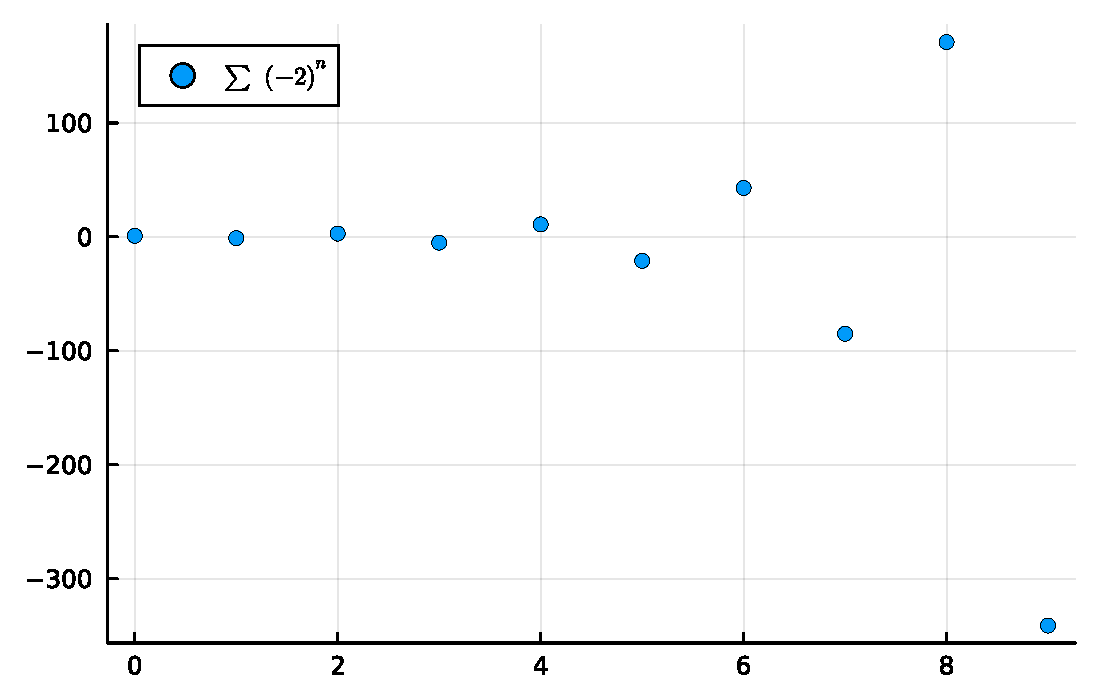
\includegraphics{index_files/mediabag/02-sucesiones_files/figure-pdf/cell-7-output-1.pdf}

\section{Makie}

\begin{Shaded}
\begin{Highlighting}[]
\ImportTok{using} \BuiltInTok{GLMakie}
\FunctionTok{a}\NormalTok{(n) }\OperatorTok{=}\NormalTok{ n }\OperatorTok{/}\NormalTok{ (}\FloatTok{4}\NormalTok{n }\OperatorTok{+} \FloatTok{2}\NormalTok{)}
\NormalTok{Makie.}\FunctionTok{scatter}\NormalTok{([}\FunctionTok{a}\NormalTok{(n) for n }\OperatorTok{=} \FloatTok{1}\OperatorTok{:}\FloatTok{50}\NormalTok{])}
\end{Highlighting}
\end{Shaded}

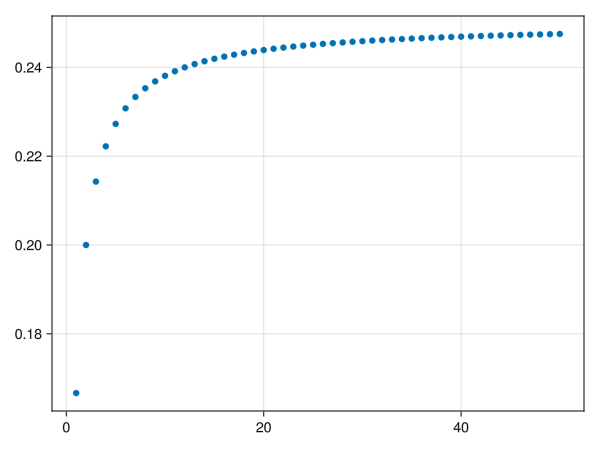
\includegraphics{02-sucesiones_files/figure-pdf/cell-8-output-1.png}

La sucesión converge al número \(0.25\).

\end{tcolorbox}

\begin{enumerate}
\def\labelenumi{\alph{enumi}.}
\setcounter{enumi}{1}
\tightlist
\item
  \(\left(\frac{2^n}{n^2}\right)_{n=1}^\infty\)
\end{enumerate}

\begin{tcolorbox}[enhanced jigsaw, bottomtitle=1mm, colframe=quarto-callout-tip-color-frame, bottomrule=.15mm, colback=white, toprule=.15mm, rightrule=.15mm, colbacktitle=quarto-callout-tip-color!10!white, left=2mm, opacitybacktitle=0.6, arc=.35mm, coltitle=black, opacityback=0, breakable, toptitle=1mm, titlerule=0mm, title=\textcolor{quarto-callout-tip-color}{\faLightbulb}\hspace{0.5em}{Solución}, leftrule=.75mm]

\section{Plots}

\begin{Shaded}
\begin{Highlighting}[]
\ImportTok{using} \BuiltInTok{Plots}
\FunctionTok{a}\NormalTok{(n) }\OperatorTok{=} \FloatTok{2}\OperatorTok{\^{}}\NormalTok{n }\OperatorTok{/}\NormalTok{ (}\FloatTok{4}\NormalTok{n }\OperatorTok{+} \FloatTok{2}\NormalTok{)}
\FunctionTok{scatter}\NormalTok{([}\FunctionTok{a}\NormalTok{(n) for n }\OperatorTok{=} \FloatTok{1}\OperatorTok{:}\FloatTok{50}\NormalTok{], legend}\OperatorTok{=}\ConstantTok{false}\NormalTok{)}
\end{Highlighting}
\end{Shaded}

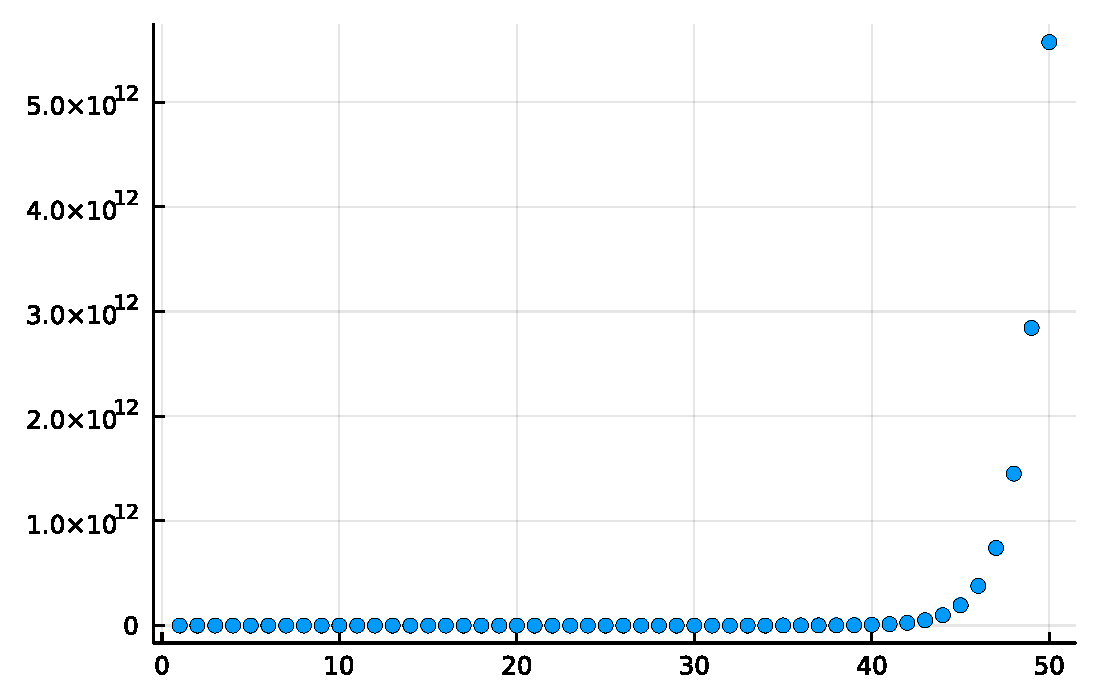
\includegraphics{index_files/mediabag/02-sucesiones_files/figure-pdf/cell-9-output-1.pdf}

\section{Makie}

\begin{Shaded}
\begin{Highlighting}[]
\ImportTok{using} \BuiltInTok{GLMakie}
\FunctionTok{a}\NormalTok{(n) }\OperatorTok{=} \FloatTok{2}\OperatorTok{\^{}}\NormalTok{n }\OperatorTok{/}\NormalTok{ (}\FloatTok{4}\NormalTok{n }\OperatorTok{+} \FloatTok{2}\NormalTok{)}
\NormalTok{Makie.}\FunctionTok{scatter}\NormalTok{([}\FunctionTok{a}\NormalTok{(n) for n }\OperatorTok{=} \FloatTok{1}\OperatorTok{:}\FloatTok{50}\NormalTok{])}
\end{Highlighting}
\end{Shaded}

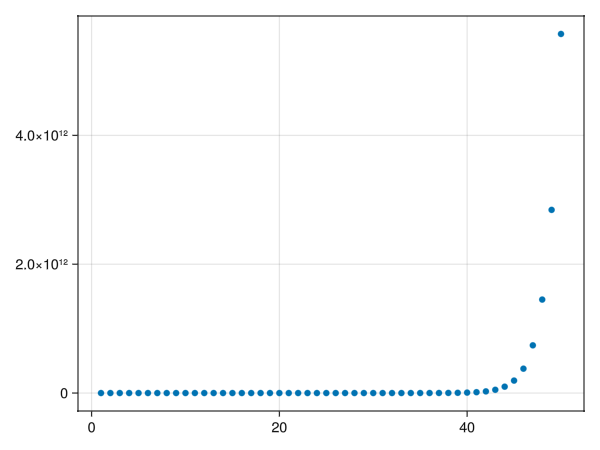
\includegraphics{02-sucesiones_files/figure-pdf/cell-10-output-1.png}

La sucesión diverge.

\end{tcolorbox}

\begin{enumerate}
\def\labelenumi{\alph{enumi}.}
\setcounter{enumi}{2}
\tightlist
\item
  \(\left(\frac{(-1)^n}{n}\right)_{n=1}^\infty\)
\end{enumerate}

\begin{tcolorbox}[enhanced jigsaw, bottomtitle=1mm, colframe=quarto-callout-tip-color-frame, bottomrule=.15mm, colback=white, toprule=.15mm, rightrule=.15mm, colbacktitle=quarto-callout-tip-color!10!white, left=2mm, opacitybacktitle=0.6, arc=.35mm, coltitle=black, opacityback=0, breakable, toptitle=1mm, titlerule=0mm, title=\textcolor{quarto-callout-tip-color}{\faLightbulb}\hspace{0.5em}{Solución}, leftrule=.75mm]

\section{Plots}

\begin{Shaded}
\begin{Highlighting}[]
\ImportTok{using} \BuiltInTok{Plots}
\FunctionTok{a}\NormalTok{(n) }\OperatorTok{=}\NormalTok{ (}\OperatorTok{{-}}\FloatTok{1}\NormalTok{)}\OperatorTok{\^{}}\NormalTok{n }\OperatorTok{/}\NormalTok{ n}
\FunctionTok{scatter}\NormalTok{([}\FunctionTok{a}\NormalTok{(n) for n }\OperatorTok{=} \FloatTok{1}\OperatorTok{:}\FloatTok{50}\NormalTok{], legend}\OperatorTok{=}\ConstantTok{false}\NormalTok{)}
\end{Highlighting}
\end{Shaded}

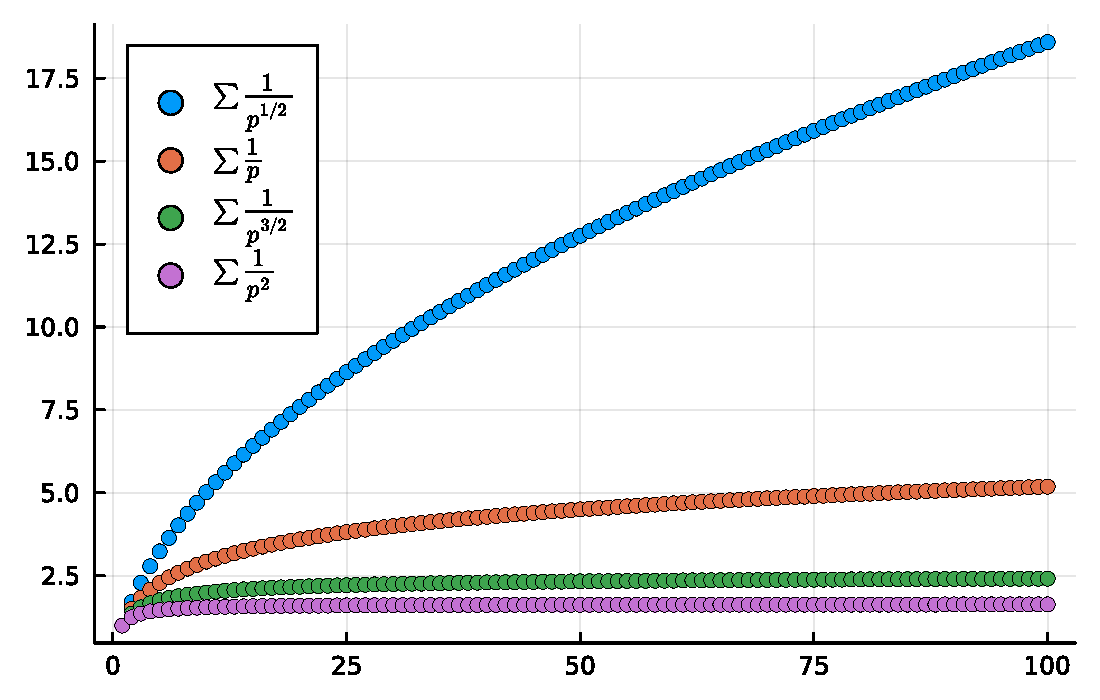
\includegraphics{index_files/mediabag/02-sucesiones_files/figure-pdf/cell-11-output-1.pdf}

\section{Makie}

\begin{Shaded}
\begin{Highlighting}[]
\ImportTok{using} \BuiltInTok{GLMakie}
\FunctionTok{a}\NormalTok{(n) }\OperatorTok{=}\NormalTok{ (}\OperatorTok{{-}}\FloatTok{1}\NormalTok{)}\OperatorTok{\^{}}\NormalTok{n }\OperatorTok{/}\NormalTok{ n}
\NormalTok{Makie.}\FunctionTok{scatter}\NormalTok{([}\FunctionTok{a}\NormalTok{(n) for n }\OperatorTok{=} \FloatTok{1}\OperatorTok{:}\FloatTok{50}\NormalTok{])}
\end{Highlighting}
\end{Shaded}

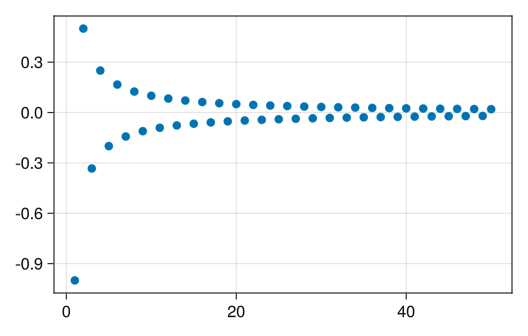
\includegraphics{02-sucesiones_files/figure-pdf/cell-12-output-1.png}

La sucesión converge al \(0\).

\end{tcolorbox}

\begin{enumerate}
\def\labelenumi{\alph{enumi}.}
\setcounter{enumi}{3}
\tightlist
\item
  \(\left(\left(1+\frac{1}{n}\right)^n\right)_{n=1}^\infty\)
\end{enumerate}

\begin{tcolorbox}[enhanced jigsaw, bottomtitle=1mm, colframe=quarto-callout-tip-color-frame, bottomrule=.15mm, colback=white, toprule=.15mm, rightrule=.15mm, colbacktitle=quarto-callout-tip-color!10!white, left=2mm, opacitybacktitle=0.6, arc=.35mm, coltitle=black, opacityback=0, breakable, toptitle=1mm, titlerule=0mm, title=\textcolor{quarto-callout-tip-color}{\faLightbulb}\hspace{0.5em}{Solución}, leftrule=.75mm]

\section{Plots}

\begin{Shaded}
\begin{Highlighting}[]
\ImportTok{using} \BuiltInTok{Plots}
\FunctionTok{a}\NormalTok{(n) }\OperatorTok{=}\NormalTok{ (}\FloatTok{1} \OperatorTok{+} \FloatTok{1} \OperatorTok{/}\NormalTok{ n)}\OperatorTok{\^{}}\NormalTok{n}
\FunctionTok{scatter}\NormalTok{([}\FunctionTok{a}\NormalTok{(n) for n }\OperatorTok{=} \FloatTok{1}\OperatorTok{:}\FloatTok{50}\NormalTok{], legend}\OperatorTok{=}\ConstantTok{false}\NormalTok{)}
\end{Highlighting}
\end{Shaded}

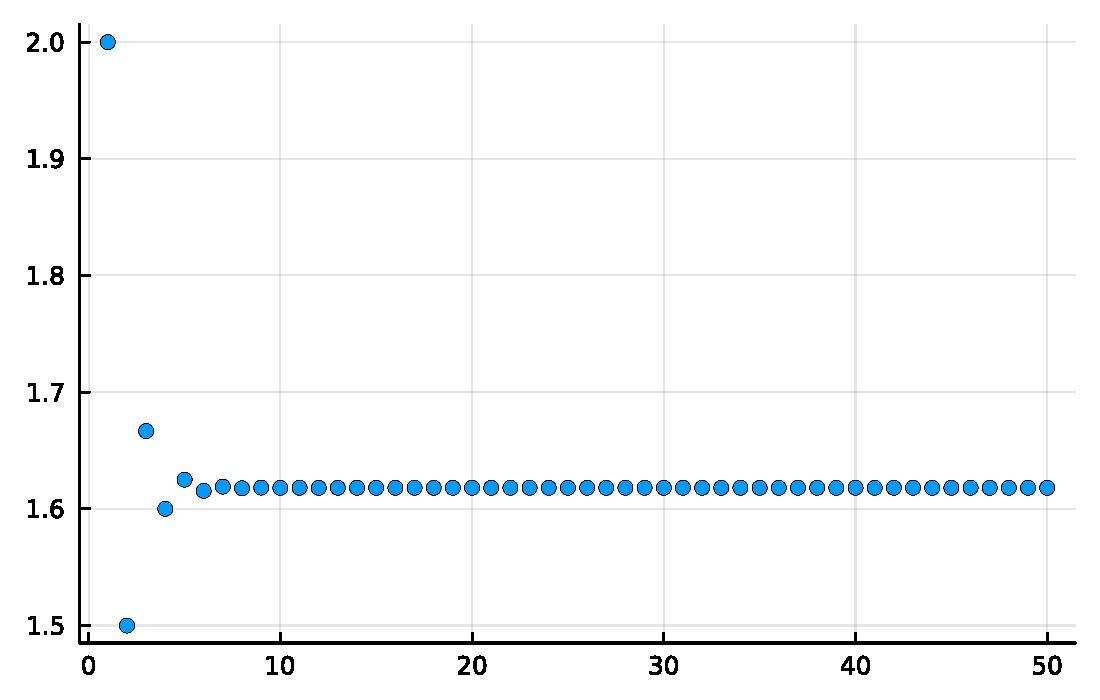
\includegraphics{index_files/mediabag/02-sucesiones_files/figure-pdf/cell-13-output-1.pdf}

\section{Makie}

\begin{Shaded}
\begin{Highlighting}[]
\ImportTok{using} \BuiltInTok{GLMakie}
\FunctionTok{a}\NormalTok{(n) }\OperatorTok{=}\NormalTok{ (}\FloatTok{1} \OperatorTok{+} \FloatTok{1} \OperatorTok{/}\NormalTok{ n)}\OperatorTok{\^{}}\NormalTok{n}
\NormalTok{Makie.}\FunctionTok{scatter}\NormalTok{([}\FunctionTok{a}\NormalTok{(n) for n }\OperatorTok{=} \FloatTok{1}\OperatorTok{:}\FloatTok{50}\NormalTok{])}
\end{Highlighting}
\end{Shaded}

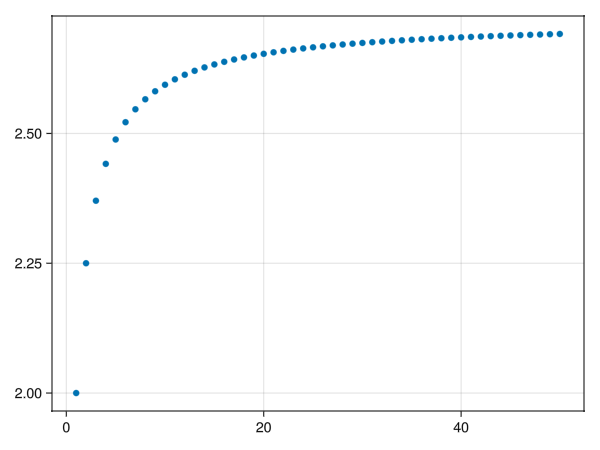
\includegraphics{02-sucesiones_files/figure-pdf/cell-14-output-1.png}

La sucesión converge aproximadamente a \(2.7\).

\end{tcolorbox}

\begin{enumerate}
\def\labelenumi{\alph{enumi}.}
\setcounter{enumi}{4}
\tightlist
\item
  \(a_1 = 0.5\) y \(a_{n+1}=\frac{3}{2+a_n}\) \(\forall n\in\mathbb{N}\)
\end{enumerate}

\begin{tcolorbox}[enhanced jigsaw, bottomtitle=1mm, colframe=quarto-callout-tip-color-frame, bottomrule=.15mm, colback=white, toprule=.15mm, rightrule=.15mm, colbacktitle=quarto-callout-tip-color!10!white, left=2mm, opacitybacktitle=0.6, arc=.35mm, coltitle=black, opacityback=0, breakable, toptitle=1mm, titlerule=0mm, title=\textcolor{quarto-callout-tip-color}{\faLightbulb}\hspace{0.5em}{Solución}, leftrule=.75mm]

\section{Plots}

\begin{Shaded}
\begin{Highlighting}[]
\ImportTok{using} \BuiltInTok{Plots}
\FunctionTok{a}\NormalTok{(n) }\OperatorTok{=}\NormalTok{  n }\OperatorTok{==} \FloatTok{1}\NormalTok{ ? }\FloatTok{0.5} \OperatorTok{:} \FloatTok{3}\OperatorTok{/}\NormalTok{(}\FloatTok{2}\FunctionTok{+a}\NormalTok{(n}\OperatorTok{{-}}\FloatTok{1}\NormalTok{))}
\FunctionTok{scatter}\NormalTok{([}\FunctionTok{a}\NormalTok{(n) for n }\OperatorTok{=} \FloatTok{1}\OperatorTok{:}\FloatTok{50}\NormalTok{], legend}\OperatorTok{=}\ConstantTok{false}\NormalTok{)}
\end{Highlighting}
\end{Shaded}

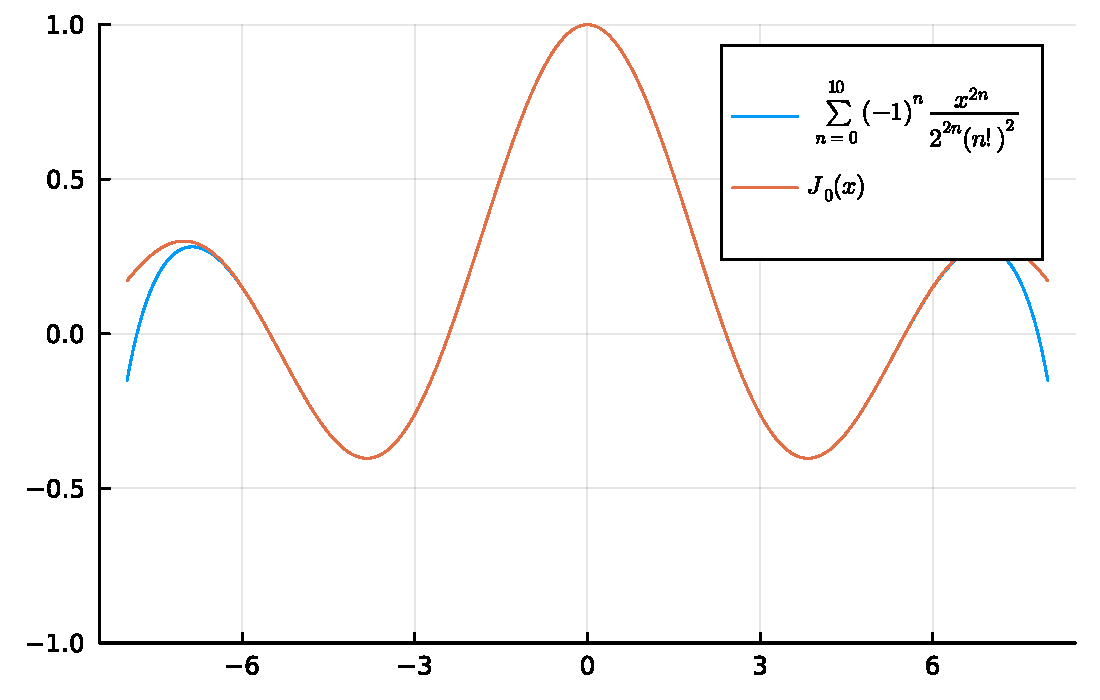
\includegraphics{index_files/mediabag/02-sucesiones_files/figure-pdf/cell-15-output-1.pdf}

\section{Makie}

\begin{Shaded}
\begin{Highlighting}[]
\ImportTok{using} \BuiltInTok{GLMakie}
\FunctionTok{a}\NormalTok{(n) }\OperatorTok{=}\NormalTok{ n }\OperatorTok{==} \FloatTok{1}\NormalTok{ ? }\FloatTok{0.5} \OperatorTok{:} \FloatTok{3}\OperatorTok{/}\NormalTok{(}\FloatTok{2}\FunctionTok{+a}\NormalTok{(n}\OperatorTok{{-}}\FloatTok{1}\NormalTok{))}
\NormalTok{Makie.}\FunctionTok{scatter}\NormalTok{([}\FunctionTok{a}\NormalTok{(n) for n }\OperatorTok{=} \FloatTok{1}\OperatorTok{:}\FloatTok{50}\NormalTok{])}
\end{Highlighting}
\end{Shaded}

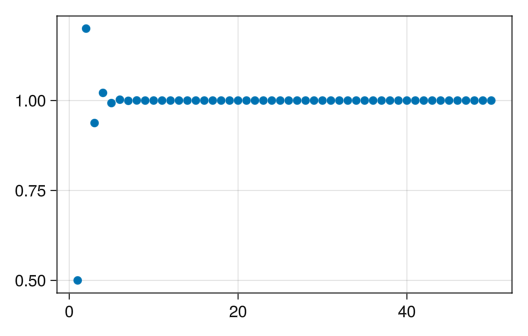
\includegraphics{02-sucesiones_files/figure-pdf/cell-16-output-1.png}

La sucesión converge aproximadamente a \(1\).

\end{tcolorbox}

\end{exercise}

\begin{exercise}[]\protect\hypertarget{exr-limite-sucesiones}{}\label{exr-limite-sucesiones}

Calcular el límite, si existe, de las siguiente sucesiones.

\begin{enumerate}
\def\labelenumi{\alph{enumi}.}
\tightlist
\item
  \(\left(\frac{1}{n}\right)_{n=1}^\infty\)
\end{enumerate}

\begin{tcolorbox}[enhanced jigsaw, bottomtitle=1mm, colframe=quarto-callout-note-color-frame, bottomrule=.15mm, colback=white, toprule=.15mm, rightrule=.15mm, colbacktitle=quarto-callout-note-color!10!white, left=2mm, opacitybacktitle=0.6, arc=.35mm, coltitle=black, opacityback=0, breakable, toptitle=1mm, titlerule=0mm, title=\textcolor{quarto-callout-note-color}{\faInfo}\hspace{0.5em}{Ayuda}, leftrule=.75mm]

Definir una función para el término general y usar la función
\href{https://docs.juliahub.com/SymPy/KzewI/1.0.31/Tutorial/calculus/\#Limits-1}{\texttt{limit}}
del paquete \texttt{SymPy} para calcular el límite de la sucesión.

\end{tcolorbox}

\begin{tcolorbox}[enhanced jigsaw, bottomtitle=1mm, colframe=quarto-callout-tip-color-frame, bottomrule=.15mm, colback=white, toprule=.15mm, rightrule=.15mm, colbacktitle=quarto-callout-tip-color!10!white, left=2mm, opacitybacktitle=0.6, arc=.35mm, coltitle=black, opacityback=0, breakable, toptitle=1mm, titlerule=0mm, title=\textcolor{quarto-callout-tip-color}{\faLightbulb}\hspace{0.5em}{Solución}, leftrule=.75mm]

\begin{Shaded}
\begin{Highlighting}[]
\ImportTok{using} \BuiltInTok{SymPy}
\PreprocessorTok{@syms}\NormalTok{ n  }\CommentTok{\# Declaración de la variable simbólica n.}
\FunctionTok{a}\NormalTok{(n) }\OperatorTok{=} \FloatTok{1}\OperatorTok{/}\NormalTok{n}
\FunctionTok{limit}\NormalTok{(}\FunctionTok{a}\NormalTok{(n), n}\OperatorTok{=\textgreater{}}\NormalTok{oo)}
\end{Highlighting}
\end{Shaded}

$0$

\end{tcolorbox}

\begin{enumerate}
\def\labelenumi{\alph{enumi}.}
\setcounter{enumi}{1}
\tightlist
\item
  \(\left((-1)^n\right)_{n=1}^\infty\)
\end{enumerate}

\begin{tcolorbox}[enhanced jigsaw, bottomtitle=1mm, colframe=quarto-callout-tip-color-frame, bottomrule=.15mm, colback=white, toprule=.15mm, rightrule=.15mm, colbacktitle=quarto-callout-tip-color!10!white, left=2mm, opacitybacktitle=0.6, arc=.35mm, coltitle=black, opacityback=0, breakable, toptitle=1mm, titlerule=0mm, title=\textcolor{quarto-callout-tip-color}{\faLightbulb}\hspace{0.5em}{Solución}, leftrule=.75mm]

\begin{Shaded}
\begin{Highlighting}[]
\PreprocessorTok{@syms}\NormalTok{ n}
\FunctionTok{a}\NormalTok{(n) }\OperatorTok{=}\NormalTok{ (}\OperatorTok{{-}}\FloatTok{1}\NormalTok{)}\OperatorTok{\^{}}\NormalTok{n}
\FunctionTok{limit}\NormalTok{(}\FunctionTok{a}\NormalTok{(n), n}\OperatorTok{=\textgreater{}}\NormalTok{oo)}
\end{Highlighting}
\end{Shaded}

$\text{NaN}$

\end{tcolorbox}

\begin{enumerate}
\def\labelenumi{\alph{enumi}.}
\setcounter{enumi}{2}
\tightlist
\item
  \(\left(\left(1+\frac{1}{n}\right)^n\right)_{n=1}^\infty\)
\end{enumerate}

\begin{tcolorbox}[enhanced jigsaw, bottomtitle=1mm, colframe=quarto-callout-tip-color-frame, bottomrule=.15mm, colback=white, toprule=.15mm, rightrule=.15mm, colbacktitle=quarto-callout-tip-color!10!white, left=2mm, opacitybacktitle=0.6, arc=.35mm, coltitle=black, opacityback=0, breakable, toptitle=1mm, titlerule=0mm, title=\textcolor{quarto-callout-tip-color}{\faLightbulb}\hspace{0.5em}{Solución}, leftrule=.75mm]

\begin{Shaded}
\begin{Highlighting}[]
\PreprocessorTok{@syms}\NormalTok{ n}
\FunctionTok{a}\NormalTok{(n) }\OperatorTok{=}\NormalTok{ (}\FloatTok{1} \OperatorTok{+} \FloatTok{1} \OperatorTok{/}\NormalTok{ n)}\OperatorTok{\^{}}\NormalTok{n}
\FunctionTok{limit}\NormalTok{(}\FunctionTok{a}\NormalTok{(n), n}\OperatorTok{=\textgreater{}}\NormalTok{oo)}
\end{Highlighting}
\end{Shaded}

$e$

\end{tcolorbox}

\end{exercise}

\begin{exercise}[]\protect\hypertarget{exr-calculo-pi}{}\label{exr-calculo-pi}

En el siglo III A.C
\href{https://es.wikipedia.org/wiki/Arqu\%C3\%ADmedes}{Arquímedes} usó
el
\href{https://es.wikipedia.org/wiki/M\%C3\%A9todo_por_agotamiento}{método
por agotamiento} para calcular el área encerrada por una circunferencia
(y de paso el valor de \(\pi\)). La idea consiste en inscribir la
circunferencia en polígonos regulares con un número de lados cada vez
mayor.

\begin{figure}[H]

{\centering 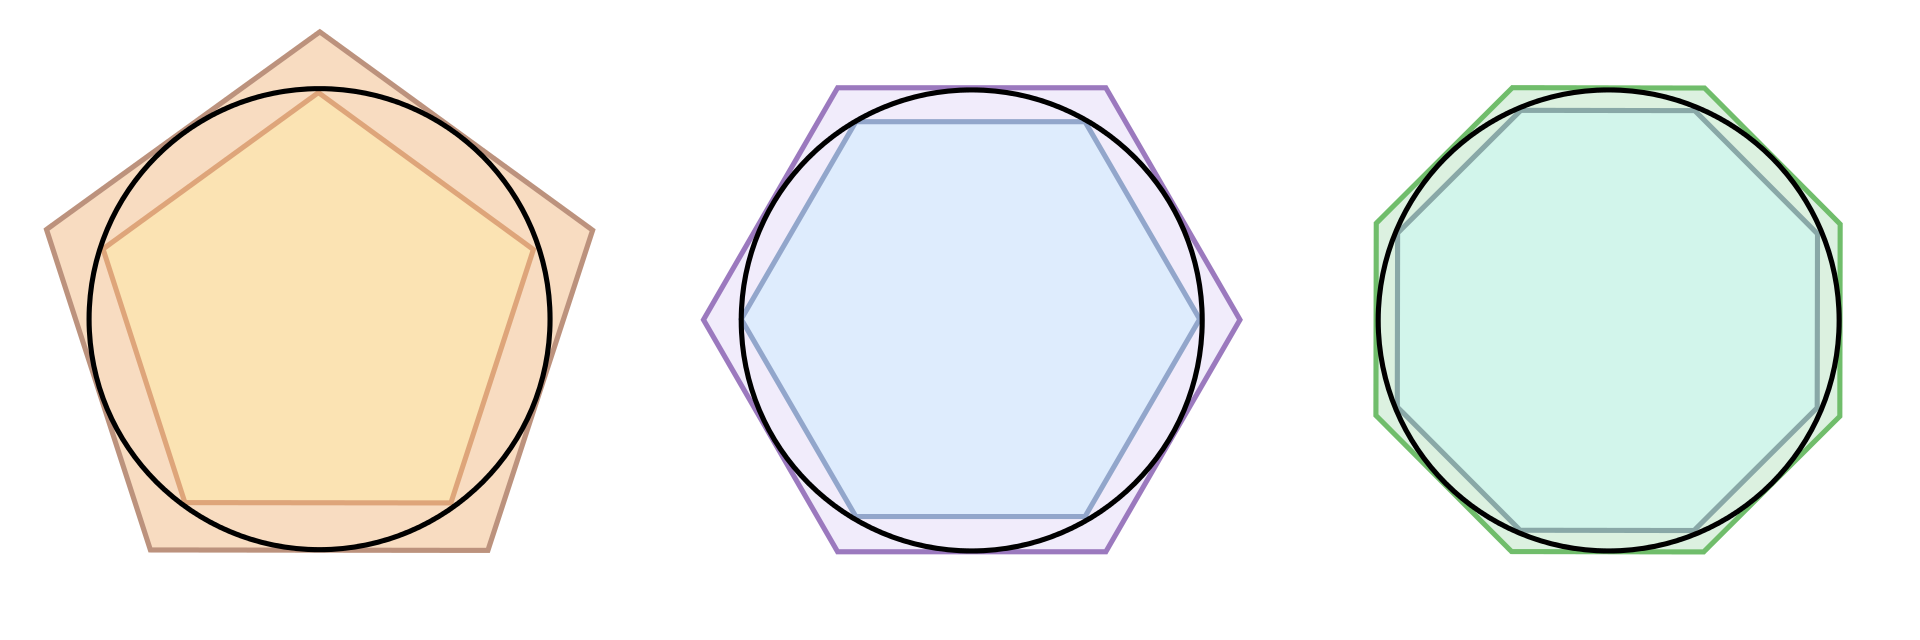
\includegraphics{img/sucesiones/poligonos-circunferencia.png}

}

\caption{Aproximación del área de una circunferencia mediante polígonos
regulares}

\end{figure}%

El área de estos polígonos puede calcularse fácilmente descomponiendo
los polígonos regulares en triángulos como en el siguiente ejemplo.

\begin{figure}
\centering
\usetikzlibrary{shapes.geometric}
\usetikzlibrary{angles}
\definecolor{myblue}{rgb}{0.067,0.529,0.871}
\definecolor{mypurple}{rgb}{0.859,0.071,0.525}
\definecolor{myred}{rgb}{1.0, 0.13, 0.32}
\definecolor{mygreen}{rgb}{0.01, 0.75, 0.24}
\def\PolyRadius{2cm}
\begin{tikzpicture}[draw=myblue, text=myblue]
\draw (0,0) circle (2);
\coordinate (A) at (-1,-1.74);
\coordinate (B) at (0,0);
\coordinate (C) at (1,-1.74);
\fill[fill=red!20] (0,0) -- (-1,-1.74) -- (1, -1.74) -- (0,0);
\node[regular polygon,draw,regular polygon sides = 6,minimum size=2*\PolyRadius] at (0,0) {};
\draw pic[draw,angle radius=0.5cm]{angle=A--B--C};
\node at (0,-0.35) {\scriptsize $\alpha$};
\draw [dashed] (0,0) -- (2,0);
\draw [dashed] (0,0) -- (-2,0);
\draw [dashed] (0,0) -- (1,1.74);
\draw [dashed] (0,0) -- (-1,1.74);
\draw [dashed] (0,0) -- (-1,-1.74);
\draw [dashed] (0,0) -- (1,-1.74) node[right, midway] {$r$};
\end{tikzpicture}

\caption{Descomposición de un hexágono en triángulos}
\end{figure}

En el caso de los polígonos inscritos dentro de la circunferencia, como
dos de los lados siempre coinciden con el radio de la circunferencia
\(r\), el perímetro del polígon de \(n\) lados puede calcularse con la
fórmula

\[
p_n = 2nr\operatorname{sen}\left(\frac{\pi}{n}\right)
\]

y el área puede calcularse con la fórmula

\[
a_n = \frac{1}{2}nr^2\operatorname{sen}\left(\frac{2\pi}{n}\right).
\]

\begin{enumerate}
\def\labelenumi{\alph{enumi}.}
\tightlist
\item
  Calcular el perímetro de los polígonos de e \(10^i\) lados, para
  \(i=1,\ldots, 6\) tomando \(r=1\).
\end{enumerate}

\begin{tcolorbox}[enhanced jigsaw, bottomtitle=1mm, colframe=quarto-callout-tip-color-frame, bottomrule=.15mm, colback=white, toprule=.15mm, rightrule=.15mm, colbacktitle=quarto-callout-tip-color!10!white, left=2mm, opacitybacktitle=0.6, arc=.35mm, coltitle=black, opacityback=0, breakable, toptitle=1mm, titlerule=0mm, title=\textcolor{quarto-callout-tip-color}{\faLightbulb}\hspace{0.5em}{Solución}, leftrule=.75mm]

\begin{Shaded}
\begin{Highlighting}[]
\FunctionTok{p}\NormalTok{(n) }\OperatorTok{=} \FloatTok{2}\FunctionTok{n*sin}\NormalTok{(}\ConstantTok{pi}\OperatorTok{/}\NormalTok{n)}
\FunctionTok{println}\NormalTok{([}\FunctionTok{p}\NormalTok{(}\FloatTok{10}\OperatorTok{\^{}}\NormalTok{i) for i }\OperatorTok{=} \FloatTok{1}\OperatorTok{:}\FloatTok{6}\NormalTok{])}
\end{Highlighting}
\end{Shaded}

\begin{verbatim}
[6.180339887498948, 6.282151815625658, 6.283174971759127, 6.28318520382533, 6.283185306146043, 6.283185307169251]
\end{verbatim}

\end{tcolorbox}

\begin{enumerate}
\def\labelenumi{\alph{enumi}.}
\tightlist
\item
  Calcular el área de los polígonos de \(10^i\) lados, para
  \(i=1,\ldots, 6\) tomando \(r=1\).
\end{enumerate}

\begin{tcolorbox}[enhanced jigsaw, bottomtitle=1mm, colframe=quarto-callout-tip-color-frame, bottomrule=.15mm, colback=white, toprule=.15mm, rightrule=.15mm, colbacktitle=quarto-callout-tip-color!10!white, left=2mm, opacitybacktitle=0.6, arc=.35mm, coltitle=black, opacityback=0, breakable, toptitle=1mm, titlerule=0mm, title=\textcolor{quarto-callout-tip-color}{\faLightbulb}\hspace{0.5em}{Solución}, leftrule=.75mm]

\begin{Shaded}
\begin{Highlighting}[]
\FunctionTok{a}\NormalTok{(n) }\OperatorTok{=} \FunctionTok{n*sin}\NormalTok{(}\FloatTok{2}\OperatorTok{*}\ConstantTok{pi}\OperatorTok{/}\NormalTok{n)}\OperatorTok{/}\FloatTok{2}
\FunctionTok{println}\NormalTok{([}\FunctionTok{a}\NormalTok{(}\FloatTok{10}\OperatorTok{\^{}}\NormalTok{i) for i }\OperatorTok{=} \FloatTok{1}\OperatorTok{:}\FloatTok{6}\NormalTok{])}
\end{Highlighting}
\end{Shaded}

\begin{verbatim}
[2.938926261462366, 3.1395259764656687, 3.1415719827794755, 3.141592446881286, 3.141592651522708, 3.1415926535691225]
\end{verbatim}

\end{tcolorbox}

\begin{enumerate}
\def\labelenumi{\alph{enumi}.}
\tightlist
\item
  Dibujar con los primeros 50 términos de la sucesión de los perímetros
  de los polígonos tomando \(r=1\).
\end{enumerate}

\begin{tcolorbox}[enhanced jigsaw, bottomtitle=1mm, colframe=quarto-callout-tip-color-frame, bottomrule=.15mm, colback=white, toprule=.15mm, rightrule=.15mm, colbacktitle=quarto-callout-tip-color!10!white, left=2mm, opacitybacktitle=0.6, arc=.35mm, coltitle=black, opacityback=0, breakable, toptitle=1mm, titlerule=0mm, title=\textcolor{quarto-callout-tip-color}{\faLightbulb}\hspace{0.5em}{Solución}, leftrule=.75mm]

\section{Plots}

\begin{Shaded}
\begin{Highlighting}[]
\ImportTok{using} \BuiltInTok{Plots}
\FunctionTok{a}\NormalTok{(n) }\OperatorTok{=} \FloatTok{2}\FunctionTok{n*sin}\NormalTok{(}\ConstantTok{pi}\OperatorTok{/}\NormalTok{n)}
\FunctionTok{scatter}\NormalTok{([}\FunctionTok{a}\NormalTok{(n) for n }\OperatorTok{=} \FloatTok{1}\OperatorTok{:}\FloatTok{50}\NormalTok{], legend}\OperatorTok{=}\ConstantTok{false}\NormalTok{)}
\end{Highlighting}
\end{Shaded}

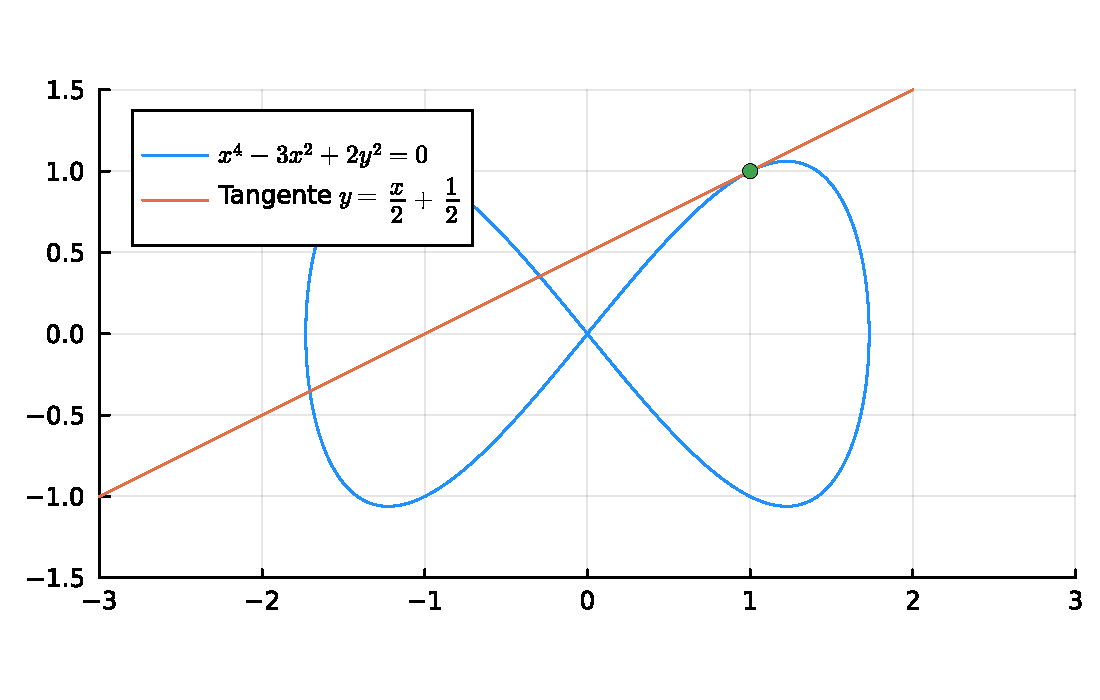
\includegraphics{index_files/mediabag/02-sucesiones_files/figure-pdf/cell-22-output-1.pdf}

\section{Makie}

\begin{Shaded}
\begin{Highlighting}[]
\ImportTok{using} \BuiltInTok{GLMakie}
\FunctionTok{a}\NormalTok{(n) }\OperatorTok{=} \FloatTok{2}\FunctionTok{n*sin}\NormalTok{(}\ConstantTok{pi}\OperatorTok{/}\NormalTok{n)}
\NormalTok{Makie.}\FunctionTok{scatter}\NormalTok{([}\FunctionTok{a}\NormalTok{(n) for n }\OperatorTok{=} \FloatTok{1}\OperatorTok{:}\FloatTok{50}\NormalTok{])}
\end{Highlighting}
\end{Shaded}

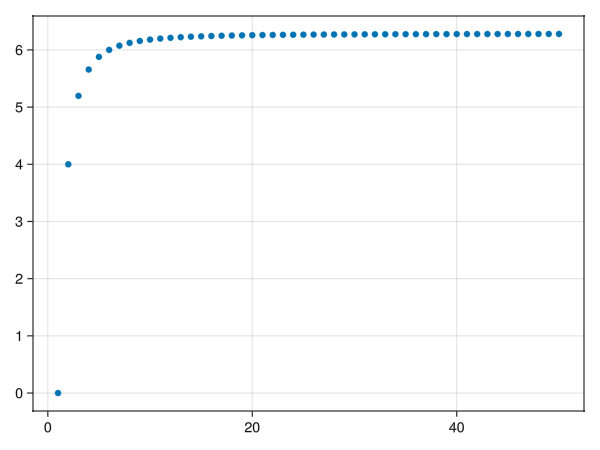
\includegraphics{02-sucesiones_files/figure-pdf/cell-23-output-1.png}

\end{tcolorbox}

\begin{enumerate}
\def\labelenumi{\alph{enumi}.}
\setcounter{enumi}{1}
\tightlist
\item
  Dibujar con los primeros 50 términos de la sucesión de las areas de
  los polígonos tomando \(r=1\).
\end{enumerate}

\begin{tcolorbox}[enhanced jigsaw, bottomtitle=1mm, colframe=quarto-callout-tip-color-frame, bottomrule=.15mm, colback=white, toprule=.15mm, rightrule=.15mm, colbacktitle=quarto-callout-tip-color!10!white, left=2mm, opacitybacktitle=0.6, arc=.35mm, coltitle=black, opacityback=0, breakable, toptitle=1mm, titlerule=0mm, title=\textcolor{quarto-callout-tip-color}{\faLightbulb}\hspace{0.5em}{Solución}, leftrule=.75mm]

\section{Plots}

\begin{Shaded}
\begin{Highlighting}[]
\ImportTok{using} \BuiltInTok{Plots}
\FunctionTok{a}\NormalTok{(n) }\OperatorTok{=} \FunctionTok{n*sin}\NormalTok{(}\FloatTok{2}\OperatorTok{*}\ConstantTok{pi}\OperatorTok{/}\NormalTok{n)}\OperatorTok{/}\FloatTok{2}
\FunctionTok{scatter}\NormalTok{([}\FunctionTok{a}\NormalTok{(n) for n }\OperatorTok{=} \FloatTok{1}\OperatorTok{:}\FloatTok{50}\NormalTok{], legend}\OperatorTok{=}\ConstantTok{false}\NormalTok{)}
\end{Highlighting}
\end{Shaded}

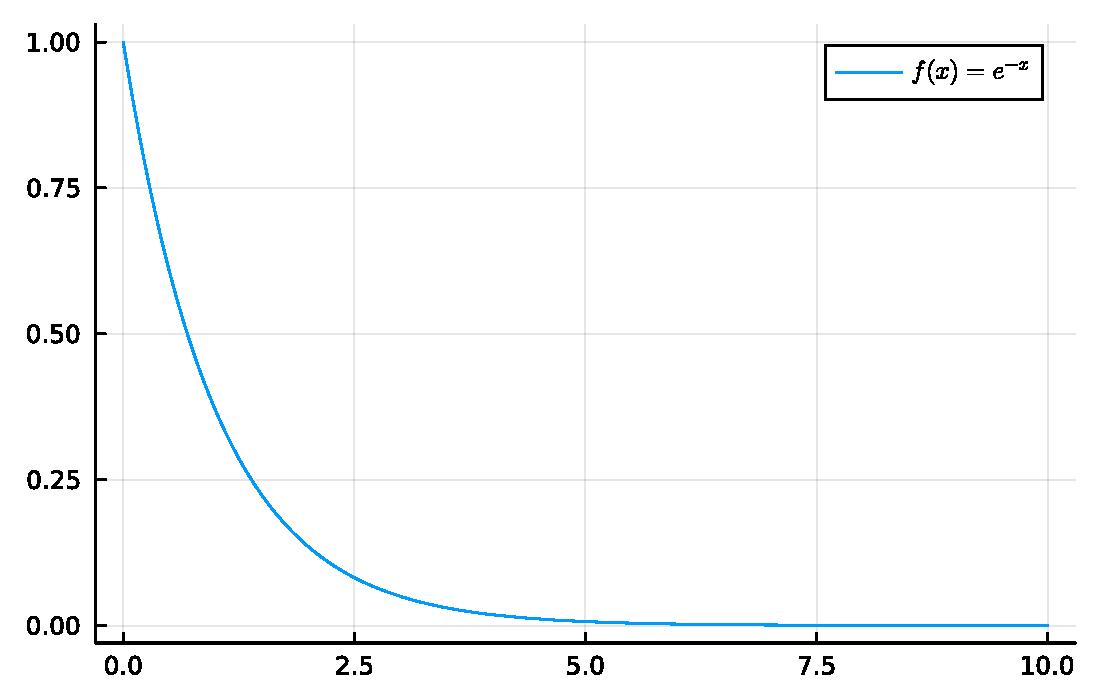
\includegraphics{index_files/mediabag/02-sucesiones_files/figure-pdf/cell-24-output-1.pdf}

\section{Makie}

\begin{Shaded}
\begin{Highlighting}[]
\ImportTok{using} \BuiltInTok{GLMakie}
\FunctionTok{a}\NormalTok{(n) }\OperatorTok{=} \FunctionTok{n*sin}\NormalTok{(}\FloatTok{2}\OperatorTok{*}\ConstantTok{pi}\OperatorTok{/}\NormalTok{n)}\OperatorTok{/}\FloatTok{2}
\NormalTok{Makie.}\FunctionTok{scatter}\NormalTok{([}\FunctionTok{a}\NormalTok{(n) for n }\OperatorTok{=} \FloatTok{1}\OperatorTok{:}\FloatTok{50}\NormalTok{])}
\end{Highlighting}
\end{Shaded}

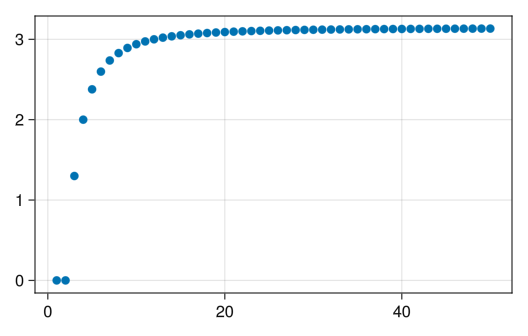
\includegraphics{02-sucesiones_files/figure-pdf/cell-25-output-1.png}

\end{tcolorbox}

\begin{enumerate}
\def\labelenumi{\alph{enumi}.}
\tightlist
\item
  Calcular el límite de la sucesión de los perímetros de los polígonos
  tomando \(r=1\).
\end{enumerate}

\begin{tcolorbox}[enhanced jigsaw, bottomtitle=1mm, colframe=quarto-callout-tip-color-frame, bottomrule=.15mm, colback=white, toprule=.15mm, rightrule=.15mm, colbacktitle=quarto-callout-tip-color!10!white, left=2mm, opacitybacktitle=0.6, arc=.35mm, coltitle=black, opacityback=0, breakable, toptitle=1mm, titlerule=0mm, title=\textcolor{quarto-callout-tip-color}{\faLightbulb}\hspace{0.5em}{Solución}, leftrule=.75mm]

\begin{Shaded}
\begin{Highlighting}[]
\ImportTok{using} \BuiltInTok{SymPy}
\PreprocessorTok{@syms}\NormalTok{ n}
\FunctionTok{a}\NormalTok{(n) }\OperatorTok{=} \FloatTok{2}\FunctionTok{n*sin}\NormalTok{(PI}\OperatorTok{/}\NormalTok{n)  }\CommentTok{\# Para cálculo simbólico es mejor utilizar la constante simbólica PI en lugar de pi.}
\FunctionTok{limit}\NormalTok{(}\FunctionTok{a}\NormalTok{(n), n}\OperatorTok{=\textgreater{}}\NormalTok{oo)}
\end{Highlighting}
\end{Shaded}

$2 \pi$

\end{tcolorbox}

\begin{enumerate}
\def\labelenumi{\alph{enumi}.}
\tightlist
\item
  Usando el resultado anterior, calcular el perímetro del círculo de
  radio \(r\).
\end{enumerate}

\begin{tcolorbox}[enhanced jigsaw, bottomtitle=1mm, colframe=quarto-callout-tip-color-frame, bottomrule=.15mm, colback=white, toprule=.15mm, rightrule=.15mm, colbacktitle=quarto-callout-tip-color!10!white, left=2mm, opacitybacktitle=0.6, arc=.35mm, coltitle=black, opacityback=0, breakable, toptitle=1mm, titlerule=0mm, title=\textcolor{quarto-callout-tip-color}{\faLightbulb}\hspace{0.5em}{Solución}, leftrule=.75mm]

\begin{Shaded}
\begin{Highlighting}[]
\ImportTok{using} \BuiltInTok{SymPy}
\PreprocessorTok{@syms}\NormalTok{ n, r}
\FunctionTok{a}\NormalTok{(n) }\OperatorTok{=} \FloatTok{2}\FunctionTok{n*r*sin}\NormalTok{(PI}\OperatorTok{/}\NormalTok{n)}
\FunctionTok{limit}\NormalTok{(}\FunctionTok{a}\NormalTok{(n), n}\OperatorTok{=\textgreater{}}\NormalTok{oo)}
\end{Highlighting}
\end{Shaded}

$2 \pi r$

\end{tcolorbox}

\begin{enumerate}
\def\labelenumi{\alph{enumi}.}
\tightlist
\item
  Calcular el límite de la sucesión de las areas de los polígonos
  tomando \(r=1\).
\end{enumerate}

\begin{tcolorbox}[enhanced jigsaw, bottomtitle=1mm, colframe=quarto-callout-tip-color-frame, bottomrule=.15mm, colback=white, toprule=.15mm, rightrule=.15mm, colbacktitle=quarto-callout-tip-color!10!white, left=2mm, opacitybacktitle=0.6, arc=.35mm, coltitle=black, opacityback=0, breakable, toptitle=1mm, titlerule=0mm, title=\textcolor{quarto-callout-tip-color}{\faLightbulb}\hspace{0.5em}{Solución}, leftrule=.75mm]

\begin{Shaded}
\begin{Highlighting}[]
\ImportTok{using} \BuiltInTok{SymPy}
\PreprocessorTok{@syms}\NormalTok{ n}
\FunctionTok{a}\NormalTok{(n) }\OperatorTok{=} \FunctionTok{n*sin}\NormalTok{(}\FloatTok{2}\OperatorTok{*}\NormalTok{PI}\OperatorTok{/}\NormalTok{n)}\OperatorTok{/}\FloatTok{2}
\FunctionTok{limit}\NormalTok{(}\FunctionTok{a}\NormalTok{(n), n}\OperatorTok{=\textgreater{}}\NormalTok{oo)}
\end{Highlighting}
\end{Shaded}

$\pi$

\end{tcolorbox}

\begin{enumerate}
\def\labelenumi{\alph{enumi}.}
\tightlist
\item
  Usando el resultado anterior, calcular el area del círculo de radio
  \(r\).
\end{enumerate}

\begin{tcolorbox}[enhanced jigsaw, bottomtitle=1mm, colframe=quarto-callout-tip-color-frame, bottomrule=.15mm, colback=white, toprule=.15mm, rightrule=.15mm, colbacktitle=quarto-callout-tip-color!10!white, left=2mm, opacitybacktitle=0.6, arc=.35mm, coltitle=black, opacityback=0, breakable, toptitle=1mm, titlerule=0mm, title=\textcolor{quarto-callout-tip-color}{\faLightbulb}\hspace{0.5em}{Solución}, leftrule=.75mm]

\begin{Shaded}
\begin{Highlighting}[]
\ImportTok{using} \BuiltInTok{SymPy}
\PreprocessorTok{@syms}\NormalTok{ n, r}
\FunctionTok{a}\NormalTok{(n) }\OperatorTok{=}\NormalTok{ n}\OperatorTok{*}\NormalTok{r}\OperatorTok{\^{}}\FloatTok{2}\FunctionTok{*sin}\NormalTok{(}\FloatTok{2}\OperatorTok{*}\NormalTok{PI}\OperatorTok{/}\NormalTok{n)}\OperatorTok{/}\FloatTok{2}
\FunctionTok{limit}\NormalTok{(}\FunctionTok{a}\NormalTok{(n), n}\OperatorTok{=\textgreater{}}\NormalTok{oo)}
\end{Highlighting}
\end{Shaded}

$\pi r^{2}$

\end{tcolorbox}

\end{exercise}

\begin{exercise}[]\protect\hypertarget{exr-subsucesiones}{}\label{exr-subsucesiones}

Dada la sucesión \(a_1=1\) y \(a_{n+1}=1+\frac{1}{a_n}\)
\(\forall n\in\mathbb{N}\), se pide:

\begin{enumerate}
\def\labelenumi{\alph{enumi}.}
\tightlist
\item
  Dibujar la gráfica de los 10 primeros términos de la sucesión. ¿Es una
  sucesión monótona?
\end{enumerate}

\begin{tcolorbox}[enhanced jigsaw, bottomtitle=1mm, colframe=quarto-callout-tip-color-frame, bottomrule=.15mm, colback=white, toprule=.15mm, rightrule=.15mm, colbacktitle=quarto-callout-tip-color!10!white, left=2mm, opacitybacktitle=0.6, arc=.35mm, coltitle=black, opacityback=0, breakable, toptitle=1mm, titlerule=0mm, title=\textcolor{quarto-callout-tip-color}{\faLightbulb}\hspace{0.5em}{Solución}, leftrule=.75mm]

\section{Plots}

\begin{Shaded}
\begin{Highlighting}[]
\ImportTok{using} \BuiltInTok{Plots}
\FunctionTok{a}\NormalTok{(n) }\OperatorTok{=}\NormalTok{  n }\OperatorTok{==} \FloatTok{1}\NormalTok{ ? }\FloatTok{1} \OperatorTok{:} \FloatTok{1} \OperatorTok{+} \FloatTok{1} \OperatorTok{/} \FunctionTok{a}\NormalTok{(n}\OperatorTok{{-}}\FloatTok{1}\NormalTok{)}
\FunctionTok{scatter}\NormalTok{([}\FunctionTok{a}\NormalTok{(n) for n }\OperatorTok{=} \FloatTok{1}\OperatorTok{:}\FloatTok{10}\NormalTok{], legend}\OperatorTok{=}\ConstantTok{false}\NormalTok{)}
\end{Highlighting}
\end{Shaded}

\includegraphics{index_files/mediabag/02-sucesiones_files/figure-pdf/cell-30-output-1.pdf}

\section{Makie}

\begin{Shaded}
\begin{Highlighting}[]
\ImportTok{using} \BuiltInTok{GLMakie}
\FunctionTok{a}\NormalTok{(n) }\OperatorTok{=}\NormalTok{ n }\OperatorTok{==} \FloatTok{1}\NormalTok{ ? }\FloatTok{1} \OperatorTok{:} \FloatTok{1} \OperatorTok{+} \FloatTok{1} \OperatorTok{/} \FunctionTok{a}\NormalTok{(n}\OperatorTok{{-}}\FloatTok{1}\NormalTok{)}
\NormalTok{Makie.}\FunctionTok{scatter}\NormalTok{([}\FunctionTok{a}\NormalTok{(n) for n }\OperatorTok{=} \FloatTok{1}\OperatorTok{:}\FloatTok{10}\NormalTok{])}
\end{Highlighting}
\end{Shaded}

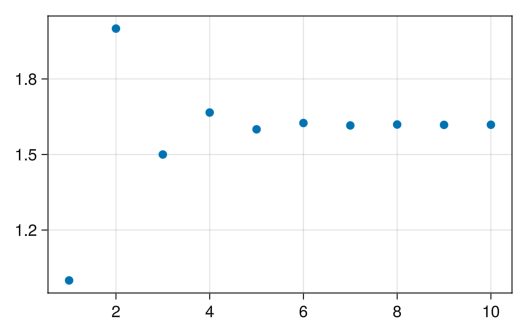
\includegraphics{02-sucesiones_files/figure-pdf/cell-31-output-1.png}

La sucesión no es monótona.

\end{tcolorbox}

\begin{enumerate}
\def\labelenumi{\alph{enumi}.}
\setcounter{enumi}{1}
\tightlist
\item
  Dibujar la gráfica de los 5 primeros términos de las subsucesiones con
  los términos pares e impares. ¿Son monótonas?
\end{enumerate}

\begin{tcolorbox}[enhanced jigsaw, bottomtitle=1mm, colframe=quarto-callout-tip-color-frame, bottomrule=.15mm, colback=white, toprule=.15mm, rightrule=.15mm, colbacktitle=quarto-callout-tip-color!10!white, left=2mm, opacitybacktitle=0.6, arc=.35mm, coltitle=black, opacityback=0, breakable, toptitle=1mm, titlerule=0mm, title=\textcolor{quarto-callout-tip-color}{\faLightbulb}\hspace{0.5em}{Solución}, leftrule=.75mm]

\section{Plots}

\begin{Shaded}
\begin{Highlighting}[]
\ImportTok{using} \BuiltInTok{Plots}\NormalTok{, }\BuiltInTok{LaTeXStrings}
\FunctionTok{a}\NormalTok{(n) }\OperatorTok{=}\NormalTok{  n }\OperatorTok{==} \FloatTok{1}\NormalTok{ ? }\FloatTok{1} \OperatorTok{:} \FloatTok{1} \OperatorTok{+} \FloatTok{1} \OperatorTok{/} \FunctionTok{a}\NormalTok{(n}\OperatorTok{{-}}\FloatTok{1}\NormalTok{)}
\NormalTok{Plots.}\FunctionTok{scatter}\NormalTok{([}\FunctionTok{a}\NormalTok{(}\FloatTok{2}\NormalTok{i}\OperatorTok{{-}}\FloatTok{1}\NormalTok{) for i}\OperatorTok{=}\FloatTok{1}\OperatorTok{:}\FloatTok{5}\NormalTok{], label }\OperatorTok{=}\NormalTok{ L}\StringTok{"}\SpecialCharTok{$}\NormalTok{a\_}\StringTok{\{2n{-}1\}}\SpecialCharTok{$}\StringTok{")}
\NormalTok{Plots}\StringTok{.scatter!([a(2i) for i=1:5], label = L"}\OperatorTok{$}\NormalTok{a\_\{}\FloatTok{2}\NormalTok{n\}}\OperatorTok{$}\StringTok{")}
\end{Highlighting}
\end{Shaded}

\includegraphics{index_files/mediabag/02-sucesiones_files/figure-pdf/cell-32-output-1.pdf}

\section{Makie}

\begin{Shaded}
\begin{Highlighting}[]
\ImportTok{using} \BuiltInTok{GLMakie}
\FunctionTok{a}\NormalTok{(n) }\OperatorTok{=}\NormalTok{ n }\OperatorTok{==} \FloatTok{1}\NormalTok{ ? }\FloatTok{1} \OperatorTok{:} \FloatTok{1} \OperatorTok{+} \FloatTok{1} \OperatorTok{/} \FunctionTok{a}\NormalTok{(n}\OperatorTok{{-}}\FloatTok{1}\NormalTok{)}
\NormalTok{fig, ax }\OperatorTok{=}\NormalTok{ Makie.}\FunctionTok{scatter}\NormalTok{([}\FunctionTok{a}\NormalTok{(}\FloatTok{2}\NormalTok{i}\OperatorTok{{-}}\FloatTok{1}\NormalTok{) for i }\OperatorTok{=} \FloatTok{1}\OperatorTok{:}\FloatTok{5}\NormalTok{], label }\OperatorTok{=}\NormalTok{ L}\StringTok{"}\SpecialCharTok{$}\NormalTok{a\_}\StringTok{\{2n{-}1\}}\SpecialCharTok{$}\StringTok{" )}
\NormalTok{Makie}\StringTok{.scatter!(ax,[a(2i) for i=1:5], label = L"}\OperatorTok{$}\NormalTok{a\_\{}\FloatTok{2}\NormalTok{n\}}\OperatorTok{$}\StringTok{")}
\FunctionTok{axislegend}\NormalTok{()}
\NormalTok{fig}
\end{Highlighting}
\end{Shaded}

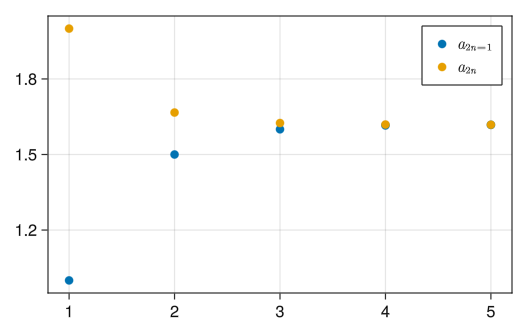
\includegraphics{02-sucesiones_files/figure-pdf/cell-33-output-1.png}

La sucesión de los términos impares es creciente y la de los pares es
decreciente.

\end{tcolorbox}

\end{exercise}

\section{Ejercicios propuestos}\label{ejercicios-propuestos}

\begin{exercise}[]\protect\hypertarget{exr-sucesiones-propuesto-1}{}\label{exr-sucesiones-propuesto-1}

Calcular el décimo término de la sucesión
\(\left(\frac{3n^2+n}{6n^2-1}\right)_{n=1}^\infty\).

\vspace{18pt}*Hint: *

Introducir hasta 5 decimales

\end{exercise}

\begin{exercise}[]\protect\hypertarget{exr-sucesiones-propuesto-2}{}\label{exr-sucesiones-propuesto-2}

Calcular los 10 primeros términos de la sucesión
\(\left(\frac{3n^2+n}{6n^2-1}\right)_{n=1}^\infty\) y averiguar hacia
dónde converge.

${\quad\Box}$ 0

${\quad\Box}$ 1.5

${\quad\Box}$ 1

${\quad\Box}$ 0.5

${\quad\Box}$ No converge

\end{exercise}

\begin{exercise}[]\protect\hypertarget{exr-sucesiones-propuesto-3}{}\label{exr-sucesiones-propuesto-3}

¿Cuál de las siguientes gráficas corresponde a la sucesión \(a_1=3\) y
\(a_{n+1}=\sqrt{2a_n}\) \(\forall n\in\mathbb{N}\).

insert image here

\end{exercise}

\begin{exercise}[]\protect\hypertarget{exr-sucesiones-propuesto-4}{}\label{exr-sucesiones-propuesto-4}

A la vista de la gráfica de los 20 primeros términos de la sucesión
\(\left(\frac{2^n}{n!}\right)_{n=1}^\infty\), ¿crees que la sucesión
converge?

${\quad\Box}$ Yes

${\quad\Box}$ No

\end{exercise}

\begin{exercise}[]\protect\hypertarget{exr-sucesiones-propuesto-5}{}\label{exr-sucesiones-propuesto-5}

A la vista de la gráfica de los 10 primeros términos de la sucesión
\(\left(\frac{n^n}{n!}\right)_{n=1}^\infty\), ¿crees que la sucesión
converge?

${\quad\Box}$ Yes

${\quad\Box}$ No

\end{exercise}

\begin{exercise}[]\protect\hypertarget{exr-sucesiones-propuesto-6}{}\label{exr-sucesiones-propuesto-6}

A la vista de la gráfica de los 20 primeros términos de la sucesión dada
por \(a_1=1\) y \(a_{n+1}=\sqrt{a_n+2}\) \(\forall n\in \mathbb{N}\),
¿crees que la sucesión converge?

${\quad\Box}$ Yes

${\quad\Box}$ No

\end{exercise}

\begin{exercise}[]\protect\hypertarget{exr-sucesiones-propuesto-7}{}\label{exr-sucesiones-propuesto-7}

¿Cuál es el límite de la sucesión
\(\left(\left(1+\frac{2}{n}\right)^n\right)_{n=1}^\infty\)

\vspace{18pt}*Hint: *

Introducir hasta 5 decimales

\end{exercise}

\bookmarksetup{startatroot}

\chapter{Funciones elementales}\label{funciones-elementales}

\section{Ejercicios Resueltos}\label{ejercicios-resueltos-1}

Para la realización de esta práctica se requieren los siguientes
paquetes:

\begin{Shaded}
\begin{Highlighting}[]
\ImportTok{using} \BuiltInTok{Plots}  \CommentTok{\# Para el dibujo de gráficas.}
\ImportTok{using} \BuiltInTok{Makie} \CommentTok{\# Para obtener gráficos interactivos.}
\ImportTok{using} \BuiltInTok{SymPy} \CommentTok{\# Para el cálculo simbólico.}
\ImportTok{using} \BuiltInTok{MTH229} \CommentTok{\# Para restringir la gráfica de una función a su dominio.}
\ImportTok{using} \BuiltInTok{LaTeXStrings}  \CommentTok{\# Para usar código LaTeX en los gráficos.}
\ImportTok{using} \BuiltInTok{Latexify}  \CommentTok{\# Para convertir expresiones a código LaTeX.}
\end{Highlighting}
\end{Shaded}

\begin{exercise}[]\protect\hypertarget{exr-grafica-funcion-tabla}{}\label{exr-grafica-funcion-tabla}

La siguiente tabla contiene el número de bacterias en un cultivo cada
hora que pasa.

\begin{longtable}[]{@{}cc@{}}
\toprule\noalign{}
Horas & Bacterias \\
\midrule\noalign{}
\endhead
\bottomrule\noalign{}
\endlastfoot
0 & 1 \\
1 & 2 \\
2 & 4 \\
3 & 8 \\
4 & 16 \\
5 & 32 \\
6 & 64 \\
7 & 128 \\
\end{longtable}

Dibujar una gráfica con la evolución del la población de bacterias.

\begin{tcolorbox}[enhanced jigsaw, bottomtitle=1mm, colframe=quarto-callout-note-color-frame, bottomrule=.15mm, colback=white, toprule=.15mm, rightrule=.15mm, colbacktitle=quarto-callout-note-color!10!white, left=2mm, opacitybacktitle=0.6, arc=.35mm, coltitle=black, opacityback=0, breakable, toptitle=1mm, titlerule=0mm, title=\textcolor{quarto-callout-note-color}{\faInfo}\hspace{0.5em}{Ayuda}, leftrule=.75mm]

Definir los valores de las horas en un vector \texttt{x} y el número de
bacterias en otro \texttt{y} y luego utilizar la función
\href{https://aprendeconalf.es/manual-julia/graficos.html\#a\%C3\%B1adir-puntos-a-una-gr\%C3\%A1fica}{\texttt{scater(x,y)}}
del paquete \texttt{Makie}, o
\href{https://aprendeconalf.es/manual-julia/graficos.html\#a\%C3\%B1adir-puntos-a-una-gr\%C3\%A1fica}{\texttt{scatter(x,y)}}
del paquete \texttt{Plots} para dibujar una gráfica de puntos.

\end{tcolorbox}

\begin{tcolorbox}[enhanced jigsaw, bottomtitle=1mm, colframe=quarto-callout-tip-color-frame, bottomrule=.15mm, colback=white, toprule=.15mm, rightrule=.15mm, colbacktitle=quarto-callout-tip-color!10!white, left=2mm, opacitybacktitle=0.6, arc=.35mm, coltitle=black, opacityback=0, breakable, toptitle=1mm, titlerule=0mm, title=\textcolor{quarto-callout-tip-color}{\faLightbulb}\hspace{0.5em}{Solución}, leftrule=.75mm]

\section{Makie}

\begin{Shaded}
\begin{Highlighting}[]
\ImportTok{using} \BuiltInTok{GLMakie}
\NormalTok{horas }\OperatorTok{=} \FloatTok{0}\OperatorTok{:}\FloatTok{7}
\NormalTok{bacterias }\OperatorTok{=}\NormalTok{ [}\FloatTok{1}\NormalTok{, }\FloatTok{2}\NormalTok{, }\FloatTok{4}\NormalTok{, }\FloatTok{8}\NormalTok{, }\FloatTok{16}\NormalTok{, }\FloatTok{32}\NormalTok{, }\FloatTok{64}\NormalTok{, }\FloatTok{128}\NormalTok{]}
\NormalTok{fig }\OperatorTok{=} \FunctionTok{Figure}\NormalTok{()}
\NormalTok{ax }\OperatorTok{=} \FunctionTok{Axis}\NormalTok{(fig[}\FloatTok{1}\NormalTok{,}\FloatTok{1}\NormalTok{], xlabel}\OperatorTok{=}\StringTok{"Horas"}\NormalTok{, ylabel}\OperatorTok{=}\StringTok{"Bacterias"}\NormalTok{, title}\OperatorTok{=}\StringTok{"Evolución de la población de bacterias"}\NormalTok{)}
\NormalTok{Makie.}\FunctionTok{scatter!}\NormalTok{(ax, horas, bacterias)}
\NormalTok{fig}
\end{Highlighting}
\end{Shaded}

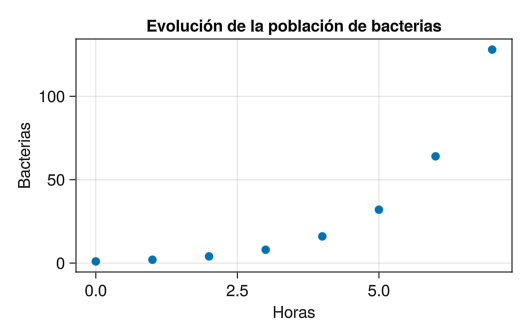
\includegraphics{03-funciones-elementales_files/figure-pdf/cell-3-output-1.png}

\section{Plots}

\begin{Shaded}
\begin{Highlighting}[]
\ImportTok{using} \BuiltInTok{Plots}
\NormalTok{horas }\OperatorTok{=} \FloatTok{0}\OperatorTok{:}\FloatTok{7}
\NormalTok{bacterias }\OperatorTok{=}\NormalTok{ [}\FloatTok{1}\NormalTok{, }\FloatTok{2}\NormalTok{, }\FloatTok{4}\NormalTok{, }\FloatTok{8}\NormalTok{, }\FloatTok{16}\NormalTok{, }\FloatTok{32}\NormalTok{, }\FloatTok{64}\NormalTok{, }\FloatTok{128}\NormalTok{]}
\NormalTok{Plots.}\FunctionTok{scatter}\NormalTok{(horas, bacterias, xlab}\OperatorTok{=}\StringTok{"Horas"}\NormalTok{, ylab}\OperatorTok{=}\StringTok{"Bacterias"}\NormalTok{, title}\OperatorTok{=}\StringTok{"Evolución de la población de bacterias"}\NormalTok{, legend}\OperatorTok{=}\ConstantTok{false}\NormalTok{)}
\end{Highlighting}
\end{Shaded}

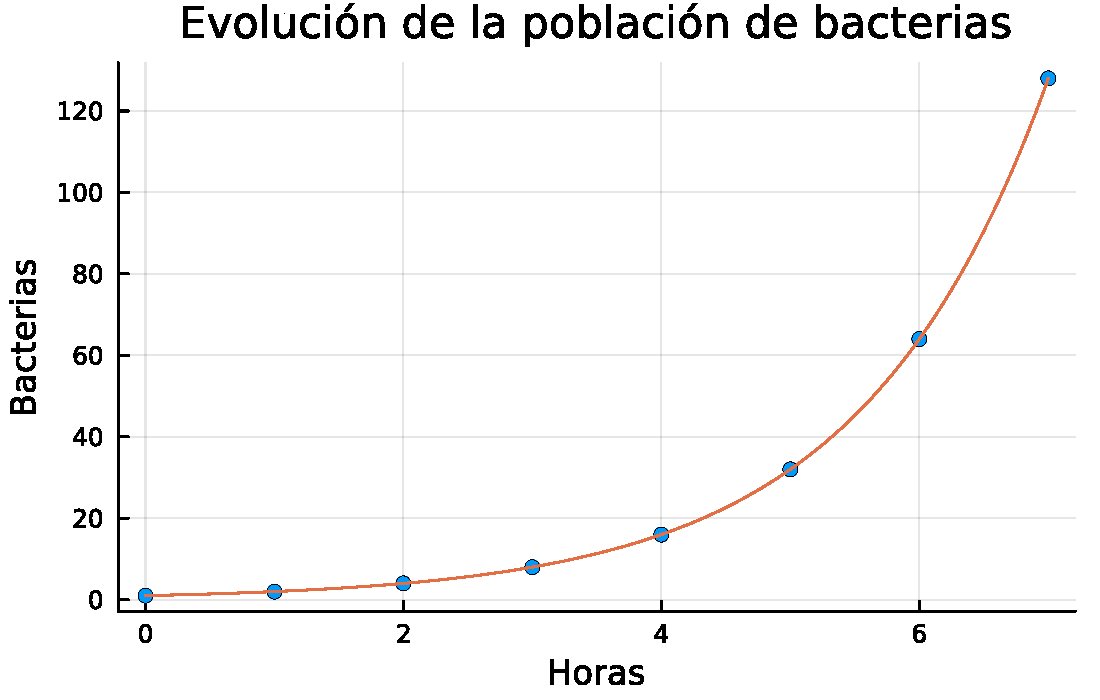
\includegraphics{index_files/mediabag/03-funciones-elementales_files/figure-pdf/cell-4-output-1.pdf}

\end{tcolorbox}

¿Los pares dados en la tabla forman una función?

\begin{tcolorbox}[enhanced jigsaw, bottomtitle=1mm, colframe=quarto-callout-tip-color-frame, bottomrule=.15mm, colback=white, toprule=.15mm, rightrule=.15mm, colbacktitle=quarto-callout-tip-color!10!white, left=2mm, opacitybacktitle=0.6, arc=.35mm, coltitle=black, opacityback=0, breakable, toptitle=1mm, titlerule=0mm, title=\textcolor{quarto-callout-tip-color}{\faLightbulb}\hspace{0.5em}{Solución}, leftrule=.75mm]

Si, porque para cada hora hay a lo sumo un número de bacterias con el
que se relaciona.

\end{tcolorbox}

¿Qué fórmula crees que explica la evolución del número de bacterias en
función de las horas que pasan? Dibuja en la gráfica anterior la función
con esa fórmula.

\begin{tcolorbox}[enhanced jigsaw, bottomtitle=1mm, colframe=quarto-callout-note-color-frame, bottomrule=.15mm, colback=white, toprule=.15mm, rightrule=.15mm, colbacktitle=quarto-callout-note-color!10!white, left=2mm, opacitybacktitle=0.6, arc=.35mm, coltitle=black, opacityback=0, breakable, toptitle=1mm, titlerule=0mm, title=\textcolor{quarto-callout-note-color}{\faInfo}\hspace{0.5em}{Ayuda}, leftrule=.75mm]

Para añadir una nueva gráfica a una anterior se añade un signo de
exclamación \texttt{!} a la función de graficación. Para una gráfica de
líneas, utilizar la función
\href{https://aprendeconalf.es/manual-julia/graficos.html\#diagrama-de-l\%C3\%ADneas}{\texttt{lines!}}
del paquete \texttt{Makie}, o
\href{https://aprendeconalf.es/manual-julia/graficos.html\#gr\%C3\%A1fica-de-una-funci\%C3\%B3n-de-una-variable}{\texttt{plot!}}
del paquete \texttt{Plots}, pasándole el nombre de la función si se ha
definido previamente o la
\href{https://aprendeconalf.es/manual-julia/funciones.html\#funciones-an\%C3\%B3nimas}{definición
anónima de la función}

\end{tcolorbox}

\begin{tcolorbox}[enhanced jigsaw, bottomtitle=1mm, colframe=quarto-callout-tip-color-frame, bottomrule=.15mm, colback=white, toprule=.15mm, rightrule=.15mm, colbacktitle=quarto-callout-tip-color!10!white, left=2mm, opacitybacktitle=0.6, arc=.35mm, coltitle=black, opacityback=0, breakable, toptitle=1mm, titlerule=0mm, title=\textcolor{quarto-callout-tip-color}{\faLightbulb}\hspace{0.5em}{Solución}, leftrule=.75mm]

\section{Makie}

\begin{Shaded}
\begin{Highlighting}[]
\NormalTok{Makie.}\FunctionTok{lines!}\NormalTok{(ax, }\FloatTok{0}\OperatorTok{..}\FloatTok{7}\NormalTok{, x }\OperatorTok{{-}\textgreater{}} \FloatTok{2}\OperatorTok{\^{}}\NormalTok{x)}
\NormalTok{fig}
\end{Highlighting}
\end{Shaded}

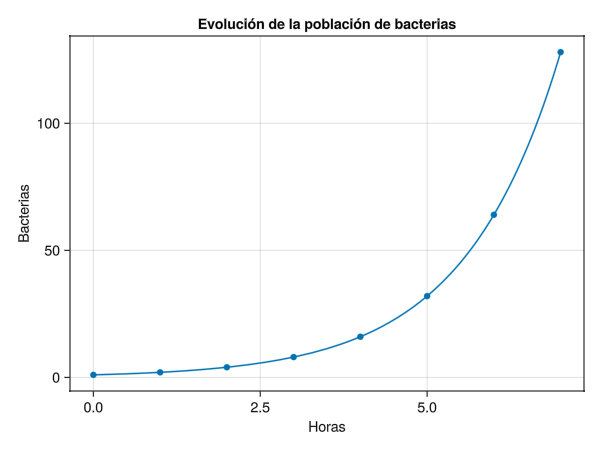
\includegraphics{03-funciones-elementales_files/figure-pdf/cell-5-output-1.png}

\section{Plots}

\begin{Shaded}
\begin{Highlighting}[]
\ImportTok{using} \BuiltInTok{Plots}
\NormalTok{Plots.}\FunctionTok{plot!}\NormalTok{(x }\OperatorTok{{-}\textgreater{}} \FloatTok{2}\OperatorTok{\^{}}\NormalTok{x)}
\end{Highlighting}
\end{Shaded}

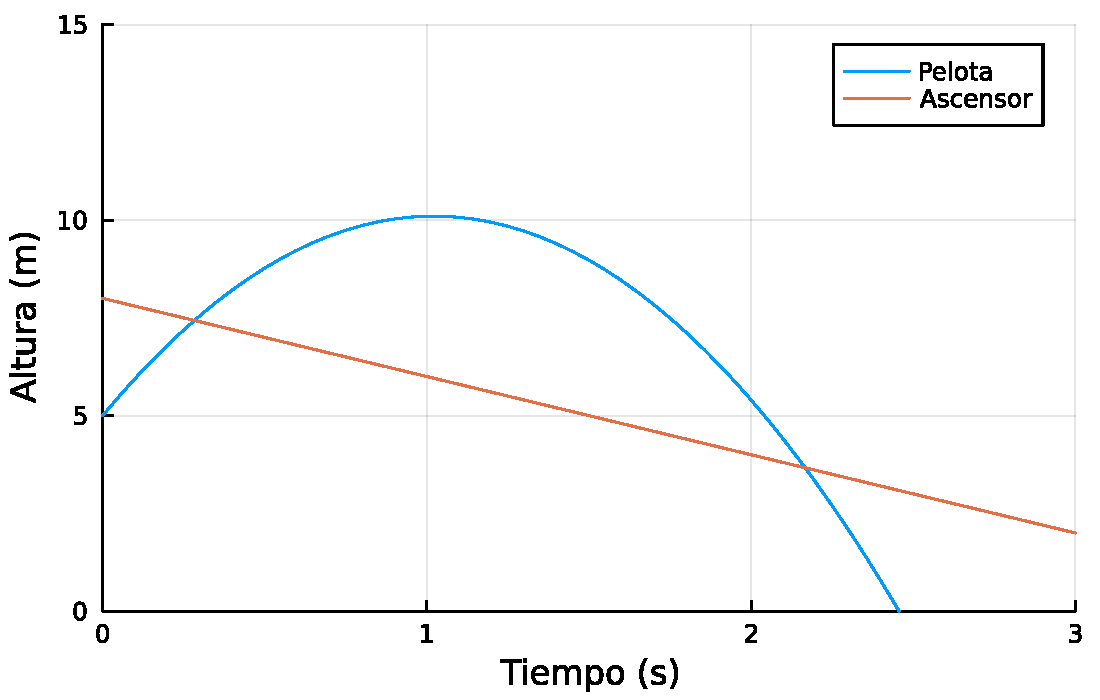
\includegraphics{index_files/mediabag/03-funciones-elementales_files/figure-pdf/cell-6-output-1.pdf}

\end{tcolorbox}

\end{exercise}

\begin{exercise}[]\protect\hypertarget{exr-resolucion-grafica-ecuacion}{}\label{exr-resolucion-grafica-ecuacion}

En el lanzamiento vertical de un objeto, la posición que ocupa el objeto
en cada instante \(t\), viene dado por la función

\[
y(t) =  y_0+v_0t+\frac{1}{2}gt^2
\]

donde \(y_0\) es la altura inicial del objeto, \(v_0\) la velocidad
inicial con que se lanza, y \(g\) es la aceleración de la gravedad. Una
pelota se lanza verticalmente desde la ventada de un edificio a 5 m de
altura, con una velocidad inicial de \(10\) m/s. Dibujar la gráfica de
la posición de la pelota en función del tiempo, tomando una aceleración
de la gravedad \(g=-9.8\) m/s².

\begin{tcolorbox}[enhanced jigsaw, bottomtitle=1mm, colframe=quarto-callout-note-color-frame, bottomrule=.15mm, colback=white, toprule=.15mm, rightrule=.15mm, colbacktitle=quarto-callout-note-color!10!white, left=2mm, opacitybacktitle=0.6, arc=.35mm, coltitle=black, opacityback=0, breakable, toptitle=1mm, titlerule=0mm, title=\textcolor{quarto-callout-note-color}{\faInfo}\hspace{0.5em}{Ayuda}, leftrule=.75mm]

Declarar \(t\) como una variable simbólica usando el paquete
\href{https://docs.juliahub.com/SymPy/KzewI/1.0.29/introduction/\#Symbols-1}{\texttt{SymPy}},
definir después las constantes \(y_0\), \(v_0\) y \(g\), y luego definir
la función \(y(t)\) mediante la fórmula dada.

Para dibujar la gráfica de la función, usar la función
\href{https://aprendeconalf.es/manual-julia/graficos.html\#diagrama-de-l\%C3\%ADneas}{lines!}
del paquete \texttt{Makie} o la función \texttt{plot} del paquete
\texttt{Plots}, pasándole el nombre de la función. Como no tienen
sentido los instantes negativos, ni las posiciones negativas, restringir
la ventana de graficación a valores de \(t\) y de \(y\) positivos usando
los parámetros
\href{https://aprendeconalf.es/manual-julia/graficos.html\#ventana-de-graficaci\%C3\%B3n}{\texttt{xlim}}
e
\href{https://aprendeconalf.es/manual-julia/graficos.html\#ventana-de-graficaci\%C3\%B3n}{\texttt{ylim}}.

\end{tcolorbox}

\begin{tcolorbox}[enhanced jigsaw, bottomtitle=1mm, colframe=quarto-callout-tip-color-frame, bottomrule=.15mm, colback=white, toprule=.15mm, rightrule=.15mm, colbacktitle=quarto-callout-tip-color!10!white, left=2mm, opacitybacktitle=0.6, arc=.35mm, coltitle=black, opacityback=0, breakable, toptitle=1mm, titlerule=0mm, title=\textcolor{quarto-callout-tip-color}{\faLightbulb}\hspace{0.5em}{Solución}, leftrule=.75mm]

\section{Makie}

\begin{Shaded}
\begin{Highlighting}[]
\ImportTok{using} \BuiltInTok{GLMakie}\NormalTok{, }\BuiltInTok{SymPy}
\PreprocessorTok{@syms}\NormalTok{ t  }\CommentTok{\#Declaramos t como una variable simbólica}
\NormalTok{y₀ }\OperatorTok{=} \FloatTok{5}
\NormalTok{v₀ }\OperatorTok{=} \FloatTok{10}
\KeywordTok{const}\NormalTok{ gravedad }\OperatorTok{=} \OperatorTok{{-}}\FloatTok{9.8}  \CommentTok{\#Declaramos la gravedad como una constante}
\FunctionTok{y0}\NormalTok{(t) }\OperatorTok{=}\NormalTok{ y₀}\OperatorTok{+}\NormalTok{v₀}\OperatorTok{*}\NormalTok{t}\OperatorTok{+} \FloatTok{1}\OperatorTok{/}\FloatTok{2}\OperatorTok{*}\NormalTok{gravedad}\OperatorTok{*}\NormalTok{t}\OperatorTok{\^{}}\FloatTok{2}
\NormalTok{fig }\OperatorTok{=} \FunctionTok{Figure}\NormalTok{()}
\NormalTok{ax }\OperatorTok{=} \FunctionTok{Axis}\NormalTok{(fig[}\FloatTok{1}\NormalTok{,}\FloatTok{1}\NormalTok{], limits}\OperatorTok{=}\NormalTok{(}\FloatTok{0}\NormalTok{, }\FloatTok{3}\NormalTok{, }\FloatTok{0}\NormalTok{, }\FloatTok{15}\NormalTok{), xlabel}\OperatorTok{=}\StringTok{"Tiempo (s)"}\NormalTok{, ylabel}\OperatorTok{=}\StringTok{"Altura (m)"}\NormalTok{)}
\NormalTok{Makie.}\FunctionTok{lines!}\NormalTok{(ax, }\FloatTok{0}\OperatorTok{..}\FloatTok{3}\NormalTok{, y0, label}\OperatorTok{=}\StringTok{"Pelota"}\NormalTok{)}
\NormalTok{fig}
\end{Highlighting}
\end{Shaded}

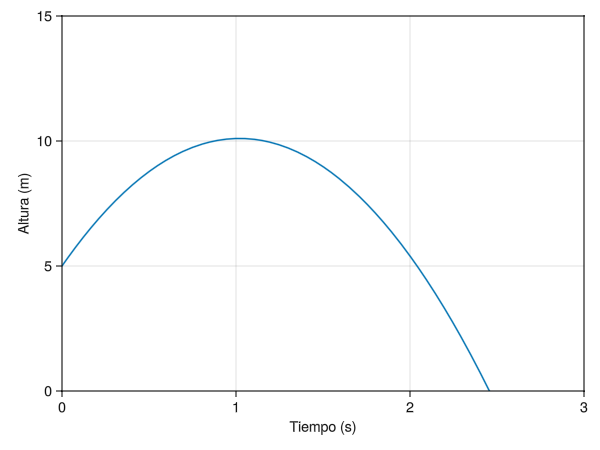
\includegraphics{03-funciones-elementales_files/figure-pdf/cell-7-output-1.png}

\section{Plots}

\begin{Shaded}
\begin{Highlighting}[]
\ImportTok{using} \BuiltInTok{Plots}\NormalTok{, }\BuiltInTok{SymPy}
\PreprocessorTok{@syms}\NormalTok{ t  }\CommentTok{\#Declaramos t como una variable simbólica}
\NormalTok{y₀ }\OperatorTok{=} \FloatTok{5}
\NormalTok{v₀ }\OperatorTok{=} \FloatTok{10}
\KeywordTok{const}\NormalTok{ gravedad }\OperatorTok{=} \OperatorTok{{-}}\FloatTok{9.8}  \CommentTok{\#Declaramos la gravedad como una constante}
\FunctionTok{y0}\NormalTok{(t) }\OperatorTok{=}\NormalTok{ y₀}\OperatorTok{+}\NormalTok{v₀}\OperatorTok{*}\NormalTok{t}\OperatorTok{+} \FloatTok{1}\OperatorTok{/}\FloatTok{2}\OperatorTok{*}\NormalTok{gravedad}\OperatorTok{*}\NormalTok{t}\OperatorTok{\^{}}\FloatTok{2}
\NormalTok{Plots.}\FunctionTok{plot}\NormalTok{(y0, xlims}\OperatorTok{=}\NormalTok{(}\FloatTok{0}\NormalTok{,}\FloatTok{3}\NormalTok{), ylims}\OperatorTok{=}\NormalTok{(}\FloatTok{0}\NormalTok{,}\FloatTok{15}\NormalTok{), label}\OperatorTok{=}\StringTok{"Pelota"}\NormalTok{, xlab}\OperatorTok{=}\StringTok{"Tiempo (s)"}\NormalTok{, ylab}\OperatorTok{=}\StringTok{"Altura (m)"}\NormalTok{)}
\end{Highlighting}
\end{Shaded}

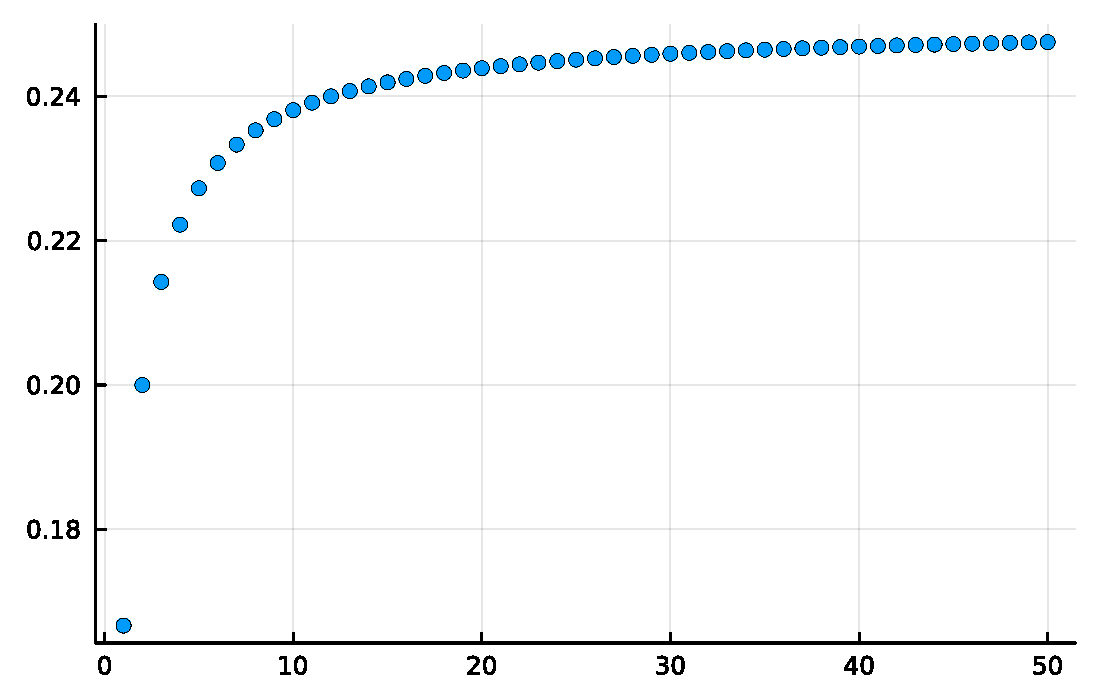
\includegraphics{index_files/mediabag/03-funciones-elementales_files/figure-pdf/cell-8-output-1.pdf}

\end{tcolorbox}

Al mismo tiempo que se lanza la pelota, un ascensor exterior baja por la
fachada del mismo edificio desde una altura de \(8\) m con una velocidad
constante de \(2\) m/s. Dibujar la gráfica de la posición del ascensor
junto a la gráfica de la pelota.

\begin{tcolorbox}[enhanced jigsaw, bottomtitle=1mm, colframe=quarto-callout-note-color-frame, bottomrule=.15mm, colback=white, toprule=.15mm, rightrule=.15mm, colbacktitle=quarto-callout-note-color!10!white, left=2mm, opacitybacktitle=0.6, arc=.35mm, coltitle=black, opacityback=0, breakable, toptitle=1mm, titlerule=0mm, title=\textcolor{quarto-callout-note-color}{\faInfo}\hspace{0.5em}{Ayuda}, leftrule=.75mm]

La función que define la posición del ascensor que baja desde una altura
\(y_1\) con una velocidad constante \(v_1\) en cada instante \(t\) es
\(y(t) = y_1-v_1t\).

\end{tcolorbox}

\begin{tcolorbox}[enhanced jigsaw, bottomtitle=1mm, colframe=quarto-callout-tip-color-frame, bottomrule=.15mm, colback=white, toprule=.15mm, rightrule=.15mm, colbacktitle=quarto-callout-tip-color!10!white, left=2mm, opacitybacktitle=0.6, arc=.35mm, coltitle=black, opacityback=0, breakable, toptitle=1mm, titlerule=0mm, title=\textcolor{quarto-callout-tip-color}{\faLightbulb}\hspace{0.5em}{Solución}, leftrule=.75mm]

\section{Makie}

\begin{Shaded}
\begin{Highlighting}[]
\NormalTok{y₁ }\OperatorTok{=} \FloatTok{8}
\NormalTok{v₁ }\OperatorTok{=} \FloatTok{2}
\FunctionTok{y1}\NormalTok{(t) }\OperatorTok{=}\NormalTok{ y₁}\OperatorTok{{-}}\NormalTok{v₁}\OperatorTok{*}\NormalTok{t}
\NormalTok{Makie.}\FunctionTok{lines!}\NormalTok{(ax, }\FloatTok{0}\OperatorTok{..}\FloatTok{3}\NormalTok{, y1, label}\OperatorTok{=}\StringTok{"Ascensor"}\NormalTok{)}
\FunctionTok{axislegend}\NormalTok{()}
\NormalTok{fig}
\end{Highlighting}
\end{Shaded}

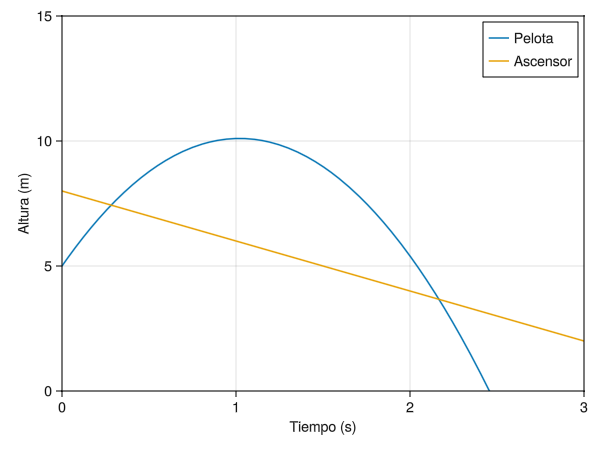
\includegraphics{03-funciones-elementales_files/figure-pdf/cell-9-output-1.png}

\section{Plots}

\begin{Shaded}
\begin{Highlighting}[]
\NormalTok{y₁ }\OperatorTok{=} \FloatTok{8}
\NormalTok{v₁ }\OperatorTok{=} \FloatTok{2}
\FunctionTok{y1}\NormalTok{(t) }\OperatorTok{=}\NormalTok{ y₁}\OperatorTok{{-}}\NormalTok{v₁}\OperatorTok{*}\NormalTok{t}
\NormalTok{Plots.}\FunctionTok{plot!}\NormalTok{(y1, label}\OperatorTok{=}\StringTok{"Ascensor"}\NormalTok{)}
\end{Highlighting}
\end{Shaded}

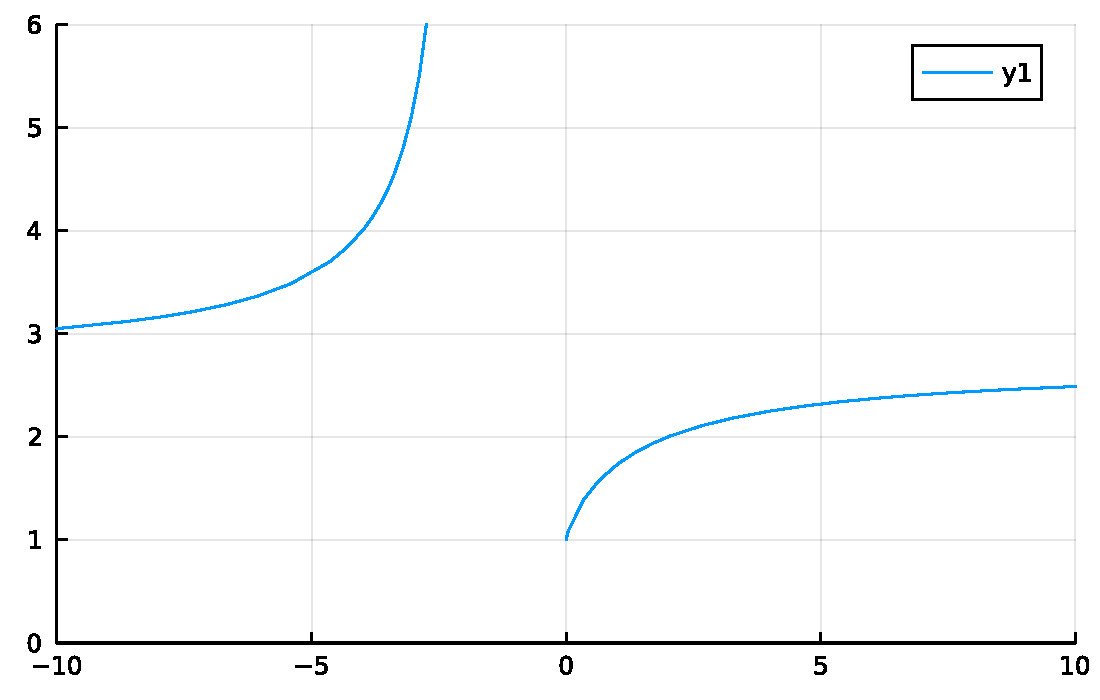
\includegraphics{index_files/mediabag/03-funciones-elementales_files/figure-pdf/cell-10-output-1.pdf}

\end{tcolorbox}

¿En qué instantes el ascensor estará a la misma altura de la pelota?
Dibujar los puntos correspondientes a esos instantes en la gráfica
anterior.

\begin{tcolorbox}[enhanced jigsaw, bottomtitle=1mm, colframe=quarto-callout-tip-color-frame, bottomrule=.15mm, colback=white, toprule=.15mm, rightrule=.15mm, colbacktitle=quarto-callout-tip-color!10!white, left=2mm, opacitybacktitle=0.6, arc=.35mm, coltitle=black, opacityback=0, breakable, toptitle=1mm, titlerule=0mm, title=\textcolor{quarto-callout-tip-color}{\faLightbulb}\hspace{0.5em}{Solución}, leftrule=.75mm]

\section{Makie}

\begin{Shaded}
\begin{Highlighting}[]
\NormalTok{sol }\OperatorTok{=} \FunctionTok{float}\NormalTok{(}\FunctionTok{solve}\NormalTok{(}\FunctionTok{y0}\NormalTok{(t)}\FunctionTok{{-}y1}\NormalTok{(t)))}
\NormalTok{Makie.}\FunctionTok{scatter!}\NormalTok{(ax, sol, }\FunctionTok{y1}\NormalTok{.(sol), color }\OperatorTok{=} \OperatorTok{:}\NormalTok{red, label}\OperatorTok{=}\StringTok{"Intersección"}\NormalTok{)}
\NormalTok{fig}
\end{Highlighting}
\end{Shaded}

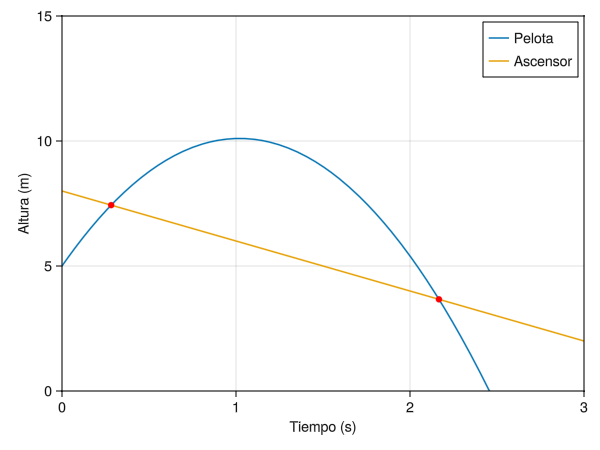
\includegraphics{03-funciones-elementales_files/figure-pdf/cell-11-output-1.png}

\section{Plots}

\begin{Shaded}
\begin{Highlighting}[]
\NormalTok{sol }\OperatorTok{=} \FunctionTok{solve}\NormalTok{(}\FunctionTok{y0}\NormalTok{(t)}\FunctionTok{{-}y1}\NormalTok{(t))}
\FunctionTok{print}\NormalTok{(}\StringTok{"Instantes: "}\NormalTok{, sol)}
\NormalTok{Plots.}\FunctionTok{scatter!}\NormalTok{(sol, }\FunctionTok{y1}\NormalTok{.(sol), label}\OperatorTok{=}\StringTok{"Intersección"}\NormalTok{)}
\end{Highlighting}
\end{Shaded}

\begin{verbatim}
Instantes: Sym{PyCall.PyObject}[0.282613815574341, 2.16636577626239]
\end{verbatim}

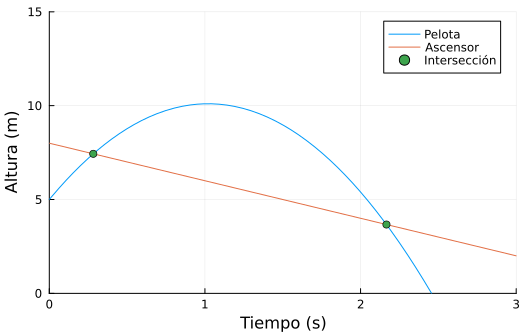
\includegraphics{index_files/mediabag/03-funciones-elementales_files/figure-pdf/cell-12-output-2.pdf}

\end{tcolorbox}

\end{exercise}

\begin{exercise}[]\protect\hypertarget{exr-grafica-funcion-polinomica}{}\label{exr-grafica-funcion-polinomica}

El volumen de un globo esférico depende del radio según la función
\(v(r)= \frac{4}{3}\pi r^3\). Calcular la función que expresa el radio
en función del volumen y dibujar su gráfica.

\begin{tcolorbox}[enhanced jigsaw, bottomtitle=1mm, colframe=quarto-callout-note-color-frame, bottomrule=.15mm, colback=white, toprule=.15mm, rightrule=.15mm, colbacktitle=quarto-callout-note-color!10!white, left=2mm, opacitybacktitle=0.6, arc=.35mm, coltitle=black, opacityback=0, breakable, toptitle=1mm, titlerule=0mm, title=\textcolor{quarto-callout-note-color}{\faInfo}\hspace{0.5em}{Ayuda}, leftrule=.75mm]

Declarar las variables simbólicas \texttt{r} y \texttt{v} usando el
paquete \texttt{SymPy} y definir la función \texttt{vol(r)} que expresa
el volumen del globo en función del radio.

Después utilizar la función
\href{https://docs.juliahub.com/SymPy/KzewI/1.0.29/introduction/\#The-solve-function-1}{\texttt{solve}}
del paquete \texttt{SymPy} para despejar \texttt{r} de la ecuación
\texttt{v-vol(r)=0}.

\end{tcolorbox}

\begin{tcolorbox}[enhanced jigsaw, bottomtitle=1mm, colframe=quarto-callout-tip-color-frame, bottomrule=.15mm, colback=white, toprule=.15mm, rightrule=.15mm, colbacktitle=quarto-callout-tip-color!10!white, left=2mm, opacitybacktitle=0.6, arc=.35mm, coltitle=black, opacityback=0, breakable, toptitle=1mm, titlerule=0mm, title=\textcolor{quarto-callout-tip-color}{\faLightbulb}\hspace{0.5em}{Solución}, leftrule=.75mm]

\section{Makie}

\begin{Shaded}
\begin{Highlighting}[]
\ImportTok{using} \BuiltInTok{GLMakie}\NormalTok{, }\BuiltInTok{SymPy}
\PreprocessorTok{@syms}\NormalTok{ r v}
\FunctionTok{vol}\NormalTok{(r) }\OperatorTok{=} \FloatTok{4}\OperatorTok{/}\FloatTok{3}\OperatorTok{*}\ConstantTok{pi}\OperatorTok{*}\NormalTok{r}\OperatorTok{\^{}}\FloatTok{3}
\NormalTok{rad }\OperatorTok{=} \FunctionTok{lambdify}\NormalTok{(}\FunctionTok{solve}\NormalTok{(}\FunctionTok{v{-}vol}\NormalTok{(r),r)[}\FloatTok{1}\NormalTok{])}
\NormalTok{fig }\OperatorTok{=} \FunctionTok{Figure}\NormalTok{()}
\NormalTok{ax }\OperatorTok{=} \FunctionTok{Axis}\NormalTok{(fig[}\FloatTok{1}\NormalTok{,}\FloatTok{1}\NormalTok{], xlabel}\OperatorTok{=}\StringTok{"Volumen (m³)"}\NormalTok{, ylabel}\OperatorTok{=}\StringTok{"Radio (m)"}\NormalTok{)}
\NormalTok{Makie.}\FunctionTok{lines!}\NormalTok{(ax, }\FloatTok{0}\OperatorTok{..}\FloatTok{10}\NormalTok{, rad)}
\NormalTok{fig}
\end{Highlighting}
\end{Shaded}

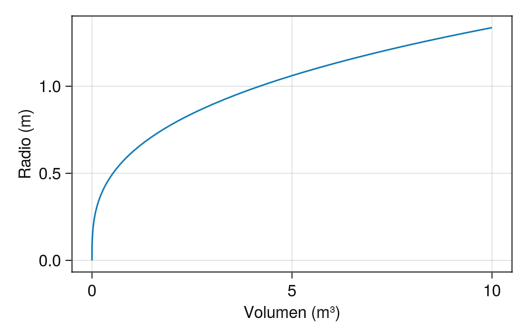
\includegraphics{03-funciones-elementales_files/figure-pdf/cell-13-output-1.png}

\section{Plots}

\begin{Shaded}
\begin{Highlighting}[]
\ImportTok{using} \BuiltInTok{Plots}\NormalTok{, }\BuiltInTok{SymPy}
\PreprocessorTok{@syms}\NormalTok{ r v}
\FunctionTok{vol}\NormalTok{(r) }\OperatorTok{=} \FloatTok{4}\OperatorTok{/}\FloatTok{3}\OperatorTok{*}\ConstantTok{pi}\OperatorTok{*}\NormalTok{r}\OperatorTok{\^{}}\FloatTok{3}
\NormalTok{rad2 }\OperatorTok{=} \FunctionTok{solve}\NormalTok{(}\FunctionTok{v{-}vol}\NormalTok{(r),r)[}\FloatTok{1}\NormalTok{]}
\NormalTok{Plots.}\FunctionTok{plot}\NormalTok{(rad2, xlim}\OperatorTok{=}\NormalTok{(}\FloatTok{0}\NormalTok{,}\FloatTok{10}\NormalTok{), xlab}\OperatorTok{=}\StringTok{"Volumen (m³)"}\NormalTok{, ylab}\OperatorTok{=}\StringTok{"Radio (m)"}\NormalTok{, legend}\OperatorTok{=}\ConstantTok{false}\NormalTok{)}
\end{Highlighting}
\end{Shaded}

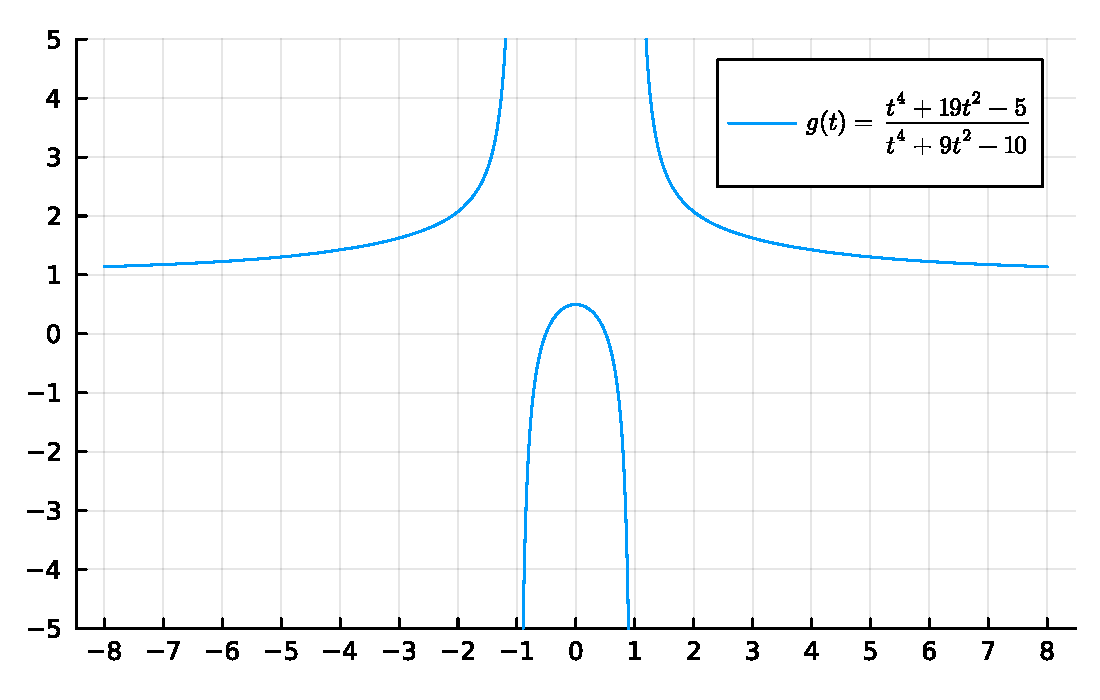
\includegraphics{index_files/mediabag/03-funciones-elementales_files/figure-pdf/cell-14-output-1.pdf}

\end{tcolorbox}

Si empezamos a introducir helio en el globo de manera que su volumen a
los \(t\) minutos viene dado por la función \(v(t)=t^2+2t\), dibujar la
gráfica de la función que da el radio en cada instante.

\begin{tcolorbox}[enhanced jigsaw, bottomtitle=1mm, colframe=quarto-callout-note-color-frame, bottomrule=.15mm, colback=white, toprule=.15mm, rightrule=.15mm, colbacktitle=quarto-callout-note-color!10!white, left=2mm, opacitybacktitle=0.6, arc=.35mm, coltitle=black, opacityback=0, breakable, toptitle=1mm, titlerule=0mm, title=\textcolor{quarto-callout-note-color}{\faInfo}\hspace{0.5em}{Ayuda}, leftrule=.75mm]

Declarar las variables simbólicas \texttt{t} usando el paquete
\texttt{SymPy} y definir la función \texttt{vol(t)} que expresa el
volumen del globo en función del tiempo.

Después utilizar a el operador de composición \(\circ\) para componer la
función del volumen con la función del radio.

\end{tcolorbox}

\begin{tcolorbox}[enhanced jigsaw, bottomtitle=1mm, colframe=quarto-callout-tip-color-frame, bottomrule=.15mm, colback=white, toprule=.15mm, rightrule=.15mm, colbacktitle=quarto-callout-tip-color!10!white, left=2mm, opacitybacktitle=0.6, arc=.35mm, coltitle=black, opacityback=0, breakable, toptitle=1mm, titlerule=0mm, title=\textcolor{quarto-callout-tip-color}{\faLightbulb}\hspace{0.5em}{Solución}, leftrule=.75mm]

\section{Makie}

\begin{Shaded}
\begin{Highlighting}[]
\ImportTok{using} \BuiltInTok{GLMakie}
\FunctionTok{vol}\NormalTok{(t)}\OperatorTok{=}\NormalTok{t}\OperatorTok{\^{}}\FloatTok{2}\OperatorTok{+}\FloatTok{2}\NormalTok{t}
\NormalTok{fig }\OperatorTok{=} \FunctionTok{Figure}\NormalTok{()}
\NormalTok{ax }\OperatorTok{=} \FunctionTok{Axis}\NormalTok{(fig[}\FloatTok{1}\NormalTok{,}\FloatTok{1}\NormalTok{], xlabel }\OperatorTok{=} \StringTok{"Tiempo (min)"}\NormalTok{, ylabel }\OperatorTok{=} \StringTok{"Radio (m)"}\NormalTok{)}
\NormalTok{Makie.}\FunctionTok{lines!}\NormalTok{(ax, }\FloatTok{0}\OperatorTok{..}\FloatTok{10}\NormalTok{, rad}\OperatorTok{∘}\NormalTok{vol)}
\NormalTok{fig}
\end{Highlighting}
\end{Shaded}

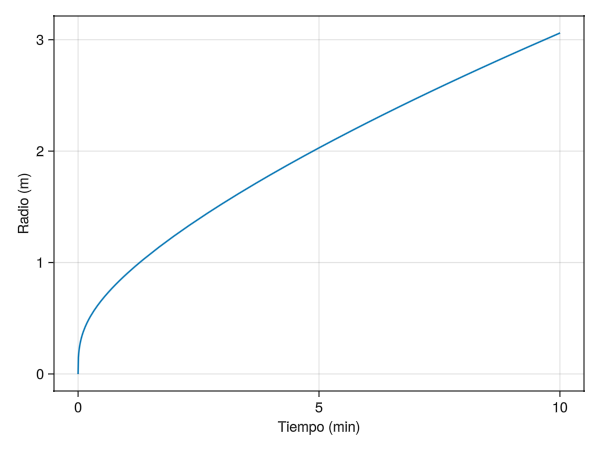
\includegraphics{03-funciones-elementales_files/figure-pdf/cell-15-output-1.png}

\section{Plots}

\begin{Shaded}
\begin{Highlighting}[]
\ImportTok{using} \BuiltInTok{Plots}\NormalTok{, }\BuiltInTok{SymPy}
\PreprocessorTok{@syms}\NormalTok{ t}
\FunctionTok{vol}\NormalTok{(t)}\OperatorTok{=}\NormalTok{t}\OperatorTok{\^{}}\FloatTok{2}\OperatorTok{+}\FloatTok{2}\NormalTok{t}
\NormalTok{Plots.}\FunctionTok{plot}\NormalTok{(rad2}\OperatorTok{∘}\NormalTok{vol, xlim }\OperatorTok{=}\NormalTok{ (}\FloatTok{0}\NormalTok{,}\FloatTok{10}\NormalTok{), xlab }\OperatorTok{=} \StringTok{"Tiempo (min)"}\NormalTok{, ylab }\OperatorTok{=} \StringTok{"Radio (m)"}\NormalTok{, legend }\OperatorTok{=} \ConstantTok{false}\NormalTok{)}
\end{Highlighting}
\end{Shaded}

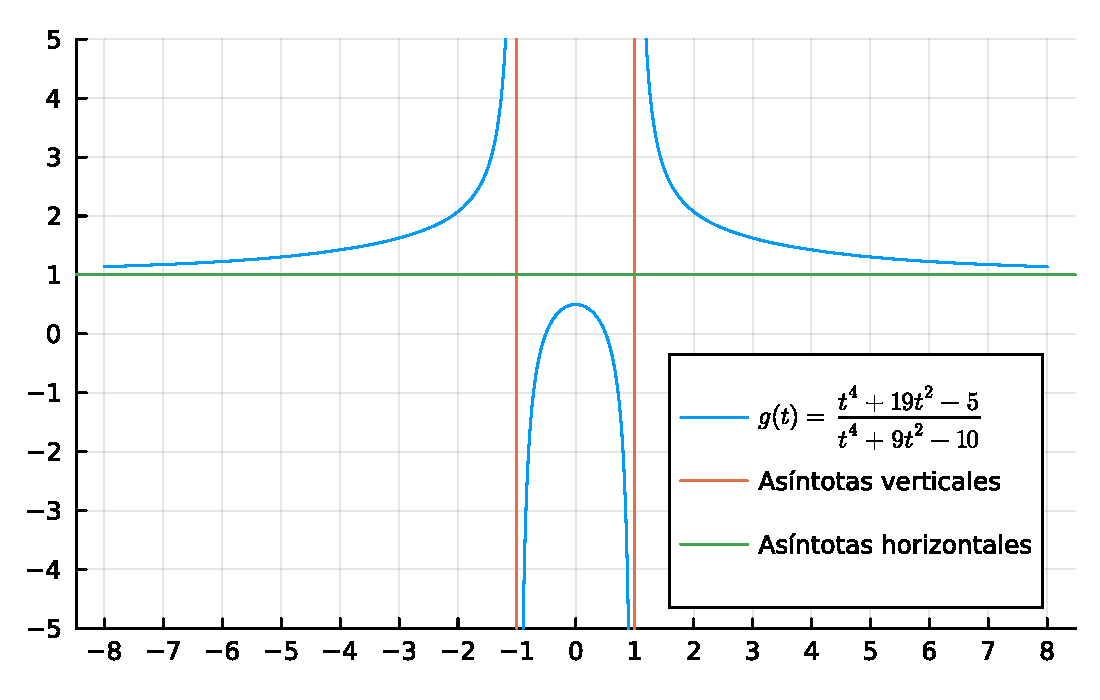
\includegraphics{index_files/mediabag/03-funciones-elementales_files/figure-pdf/cell-16-output-1.pdf}

\end{tcolorbox}

Si el globo explota cuando el radio alcanza los 3 m, ¿cuándo explotará
el globo?

\begin{tcolorbox}[enhanced jigsaw, bottomtitle=1mm, colframe=quarto-callout-tip-color-frame, bottomrule=.15mm, colback=white, toprule=.15mm, rightrule=.15mm, colbacktitle=quarto-callout-tip-color!10!white, left=2mm, opacitybacktitle=0.6, arc=.35mm, coltitle=black, opacityback=0, breakable, toptitle=1mm, titlerule=0mm, title=\textcolor{quarto-callout-tip-color}{\faLightbulb}\hspace{0.5em}{Solución}, leftrule=.75mm]

\begin{Shaded}
\begin{Highlighting}[]
\NormalTok{sol }\OperatorTok{=} \FunctionTok{solve}\NormalTok{((rad}\OperatorTok{∘}\NormalTok{vol)(t)}\OperatorTok{{-}}\FloatTok{3}\NormalTok{)}
\end{Highlighting}
\end{Shaded}

\begin{verbatim}
2-element Vector{Sym{PyCall.PyObject}}:
 -11.6816354332674
  9.68163543326738
\end{verbatim}

El globo explotará a los 9.68163543326738 minutos.

\end{tcolorbox}

\end{exercise}

\begin{exercise}[]\protect\hypertarget{exr-grafica-funcion-polinomica}{}\label{exr-grafica-funcion-polinomica}

Dibujar la gráfica de la función

\[
f(x) = 2x^3-3x^2-12x+4
\]

en el intervalo \([-3,4]\) y determinar, observando la gráfica, lo
siguiente:

\begin{tcolorbox}[enhanced jigsaw, bottomtitle=1mm, colframe=quarto-callout-note-color-frame, bottomrule=.15mm, colback=white, toprule=.15mm, rightrule=.15mm, colbacktitle=quarto-callout-note-color!10!white, left=2mm, opacitybacktitle=0.6, arc=.35mm, coltitle=black, opacityback=0, breakable, toptitle=1mm, titlerule=0mm, title=\textcolor{quarto-callout-note-color}{\faInfo}\hspace{0.5em}{Ayuda}, leftrule=.75mm]

Definir la función y usar la función usar la función
\href{https://aprendeconalf.es/manual-julia/graficos.html\#diagrama-de-l\%C3\%ADneas}{\texttt{lines!}}
del paquete \texttt{Makie} o
\href{https://docs.juliaplots.org/latest/tutorial/\#Basic-Plotting:-Line-Plots}{\texttt{plot}}
del paquete \texttt{Plots}.

\end{tcolorbox}

\begin{tcolorbox}[enhanced jigsaw, bottomtitle=1mm, colframe=quarto-callout-tip-color-frame, bottomrule=.15mm, colback=white, toprule=.15mm, rightrule=.15mm, colbacktitle=quarto-callout-tip-color!10!white, left=2mm, opacitybacktitle=0.6, arc=.35mm, coltitle=black, opacityback=0, breakable, toptitle=1mm, titlerule=0mm, title=\textcolor{quarto-callout-tip-color}{\faLightbulb}\hspace{0.5em}{Solución}, leftrule=.75mm]

\section{Makie}

\begin{Shaded}
\begin{Highlighting}[]
\ImportTok{using} \BuiltInTok{GLMakie}
\FunctionTok{f}\NormalTok{(x) }\OperatorTok{=} \FloatTok{2}\NormalTok{x}\OperatorTok{\^{}}\FloatTok{3}\OperatorTok{{-}}\FloatTok{3}\NormalTok{x}\OperatorTok{\^{}}\FloatTok{2}\OperatorTok{{-}}\FloatTok{12}\NormalTok{x}\OperatorTok{+}\FloatTok{4}
\NormalTok{fig }\OperatorTok{=} \FunctionTok{Figure}\NormalTok{()}
\NormalTok{ax }\OperatorTok{=} \FunctionTok{Axis}\NormalTok{(fig[}\FloatTok{1}\NormalTok{,}\FloatTok{1}\NormalTok{])}
\NormalTok{Makie.}\FunctionTok{lines!}\NormalTok{(ax, }\OperatorTok{{-}}\FloatTok{3}\OperatorTok{..}\FloatTok{4}\NormalTok{, f, label }\OperatorTok{=}\NormalTok{ L}\StringTok{"}\SpecialCharTok{$}\NormalTok{f}\StringTok{(x) = 2x\^{}3{-}3x\^{}2{-}12x+4}\SpecialCharTok{$}\StringTok{")}
\NormalTok{axislegend}\StringTok{()}
\NormalTok{fig}
\end{Highlighting}
\end{Shaded}

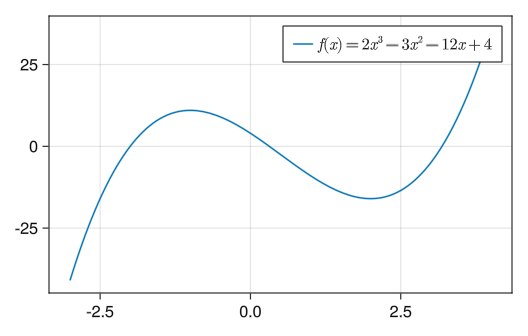
\includegraphics{03-funciones-elementales_files/figure-pdf/cell-19-output-1.png}

\section{Plots}

\begin{Shaded}
\begin{Highlighting}[]
\ImportTok{using} \BuiltInTok{Plots}\NormalTok{, }\BuiltInTok{LaTeXStrings}
\FunctionTok{f}\NormalTok{(x) }\OperatorTok{=} \FloatTok{2}\NormalTok{x}\OperatorTok{\^{}}\FloatTok{3}\OperatorTok{{-}}\FloatTok{3}\NormalTok{x}\OperatorTok{\^{}}\FloatTok{2}\OperatorTok{{-}}\FloatTok{12}\NormalTok{x}\OperatorTok{+}\FloatTok{4}
\NormalTok{Plots.}\FunctionTok{plot}\NormalTok{(f, }\OperatorTok{{-}}\FloatTok{3}\NormalTok{, }\FloatTok{4}\NormalTok{, label}\OperatorTok{=}\NormalTok{L}\StringTok{"}\SpecialCharTok{$}\NormalTok{f}\StringTok{(x) = 2x\^{}3{-}3x\^{}2{-}12x+4}\SpecialCharTok{$}\StringTok{")}
\end{Highlighting}
\end{Shaded}

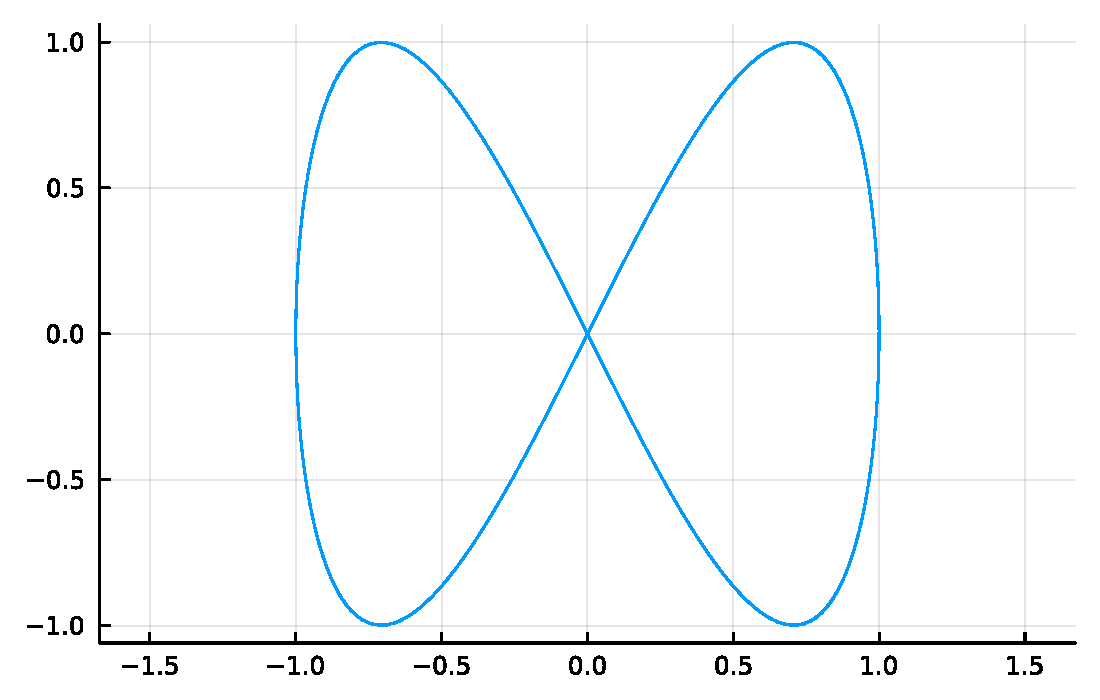
\includegraphics{index_files/mediabag/03-funciones-elementales_files/figure-pdf/cell-20-output-1.pdf}

\end{tcolorbox}

\begin{enumerate}
\def\labelenumi{\alph{enumi}.}
\tightlist
\item
  Dominio
\end{enumerate}

\begin{tcolorbox}[enhanced jigsaw, bottomtitle=1mm, colframe=quarto-callout-tip-color-frame, bottomrule=.15mm, colback=white, toprule=.15mm, rightrule=.15mm, colbacktitle=quarto-callout-tip-color!10!white, left=2mm, opacitybacktitle=0.6, arc=.35mm, coltitle=black, opacityback=0, breakable, toptitle=1mm, titlerule=0mm, title=\textcolor{quarto-callout-tip-color}{\faLightbulb}\hspace{0.5em}{Solución}, leftrule=.75mm]

\(\operatorname{Dom}(f)=\mathbb{R}\)

\end{tcolorbox}

\begin{enumerate}
\def\labelenumi{\alph{enumi}.}
\setcounter{enumi}{1}
\tightlist
\item
  Imagen
\end{enumerate}

\begin{tcolorbox}[enhanced jigsaw, bottomtitle=1mm, colframe=quarto-callout-tip-color-frame, bottomrule=.15mm, colback=white, toprule=.15mm, rightrule=.15mm, colbacktitle=quarto-callout-tip-color!10!white, left=2mm, opacitybacktitle=0.6, arc=.35mm, coltitle=black, opacityback=0, breakable, toptitle=1mm, titlerule=0mm, title=\textcolor{quarto-callout-tip-color}{\faLightbulb}\hspace{0.5em}{Solución}, leftrule=.75mm]

\(\operatorname{Im}(f)=\mathbb{R}\)

\end{tcolorbox}

\begin{enumerate}
\def\labelenumi{\alph{enumi}.}
\setcounter{enumi}{2}
\tightlist
\item
  Raíces
\end{enumerate}

\begin{tcolorbox}[enhanced jigsaw, bottomtitle=1mm, colframe=quarto-callout-tip-color-frame, bottomrule=.15mm, colback=white, toprule=.15mm, rightrule=.15mm, colbacktitle=quarto-callout-tip-color!10!white, left=2mm, opacitybacktitle=0.6, arc=.35mm, coltitle=black, opacityback=0, breakable, toptitle=1mm, titlerule=0mm, title=\textcolor{quarto-callout-tip-color}{\faLightbulb}\hspace{0.5em}{Solución}, leftrule=.75mm]

\begin{Shaded}
\begin{Highlighting}[]
\ImportTok{using} \BuiltInTok{SymPy}
\PreprocessorTok{@syms}\NormalTok{ x}
\FunctionTok{f}\NormalTok{(x) }\OperatorTok{=} \FloatTok{2}\NormalTok{x}\OperatorTok{\^{}}\FloatTok{3}\OperatorTok{{-}}\FloatTok{3}\NormalTok{x}\OperatorTok{\^{}}\FloatTok{2}\OperatorTok{{-}}\FloatTok{12}\NormalTok{x}\OperatorTok{+}\FloatTok{4}
\NormalTok{raices }\OperatorTok{=} \FunctionTok{solve}\NormalTok{(}\FunctionTok{f}\NormalTok{(x))  }\CommentTok{\# Solución exacta}
\FunctionTok{print}\NormalTok{(raices)}
\FunctionTok{N}\NormalTok{(raices)  }\CommentTok{\# Solución aproximada con decimales}
\end{Highlighting}
\end{Shaded}

\begin{verbatim}
Sym{PyCall.PyObject}[-2, 7/4 - sqrt(33)/4, sqrt(33)/4 + 7/4]
\end{verbatim}

\begin{verbatim}
3-element Vector{Sym{PyCall.PyObject}}:
               -2
 7/4 - sqrt(33)/4
 sqrt(33)/4 + 7/4
\end{verbatim}

Hay tres raíces en \(x=-2\), \(x=0.31\) y \(x=3.19\) aproximadamente.

\end{tcolorbox}

\begin{enumerate}
\def\labelenumi{\alph{enumi}.}
\setcounter{enumi}{3}
\tightlist
\item
  Signo
\end{enumerate}

\begin{tcolorbox}[enhanced jigsaw, bottomtitle=1mm, colframe=quarto-callout-tip-color-frame, bottomrule=.15mm, colback=white, toprule=.15mm, rightrule=.15mm, colbacktitle=quarto-callout-tip-color!10!white, left=2mm, opacitybacktitle=0.6, arc=.35mm, coltitle=black, opacityback=0, breakable, toptitle=1mm, titlerule=0mm, title=\textcolor{quarto-callout-tip-color}{\faLightbulb}\hspace{0.5em}{Solución}, leftrule=.75mm]

Intervalos con \(f(x)\) negativa: \((-\infty, -2)\cup (0.31,3.19)\).\\
Intervalos con \(f(x)\) positiva: \((-2,0.31)\cup (3.19,\infty)\).

\end{tcolorbox}

\begin{enumerate}
\def\labelenumi{\alph{enumi}.}
\setcounter{enumi}{4}
\tightlist
\item
  Crecimiento
\end{enumerate}

\begin{tcolorbox}[enhanced jigsaw, bottomtitle=1mm, colframe=quarto-callout-tip-color-frame, bottomrule=.15mm, colback=white, toprule=.15mm, rightrule=.15mm, colbacktitle=quarto-callout-tip-color!10!white, left=2mm, opacitybacktitle=0.6, arc=.35mm, coltitle=black, opacityback=0, breakable, toptitle=1mm, titlerule=0mm, title=\textcolor{quarto-callout-tip-color}{\faLightbulb}\hspace{0.5em}{Solución}, leftrule=.75mm]

Intervalos con \(f(x)\) creciente: \((-\infty, -1)\cup (2,\infty)\).\\
Intervalos con \(f(x)\) decreciente: \((-1,2)\).

\end{tcolorbox}

\begin{enumerate}
\def\labelenumi{\alph{enumi}.}
\setcounter{enumi}{5}
\tightlist
\item
  Extremos
\end{enumerate}

\begin{tcolorbox}[enhanced jigsaw, bottomtitle=1mm, colframe=quarto-callout-tip-color-frame, bottomrule=.15mm, colback=white, toprule=.15mm, rightrule=.15mm, colbacktitle=quarto-callout-tip-color!10!white, left=2mm, opacitybacktitle=0.6, arc=.35mm, coltitle=black, opacityback=0, breakable, toptitle=1mm, titlerule=0mm, title=\textcolor{quarto-callout-tip-color}{\faLightbulb}\hspace{0.5em}{Solución}, leftrule=.75mm]

Máximo relativo en \(x=-1\) y el valor máximo es \(f(-1)=11\).\\
Mínimo relativo en \(x=2\) y el valor del mínimo es \(f(2)=-16\).

\end{tcolorbox}

\begin{enumerate}
\def\labelenumi{\alph{enumi}.}
\setcounter{enumi}{6}
\tightlist
\item
  Concavidad
\end{enumerate}

\begin{tcolorbox}[enhanced jigsaw, bottomtitle=1mm, colframe=quarto-callout-tip-color-frame, bottomrule=.15mm, colback=white, toprule=.15mm, rightrule=.15mm, colbacktitle=quarto-callout-tip-color!10!white, left=2mm, opacitybacktitle=0.6, arc=.35mm, coltitle=black, opacityback=0, breakable, toptitle=1mm, titlerule=0mm, title=\textcolor{quarto-callout-tip-color}{\faLightbulb}\hspace{0.5em}{Solución}, leftrule=.75mm]

Intervalos de concavidad hacia arriba: \((0.5,\infty)\).\\
Intervalos de concavidad hacia abajo: \((-\infty, 0.5)\).

\end{tcolorbox}

\begin{enumerate}
\def\labelenumi{\alph{enumi}.}
\setcounter{enumi}{7}
\tightlist
\item
  Puntos de inflexión
\end{enumerate}

\begin{tcolorbox}[enhanced jigsaw, bottomtitle=1mm, colframe=quarto-callout-tip-color-frame, bottomrule=.15mm, colback=white, toprule=.15mm, rightrule=.15mm, colbacktitle=quarto-callout-tip-color!10!white, left=2mm, opacitybacktitle=0.6, arc=.35mm, coltitle=black, opacityback=0, breakable, toptitle=1mm, titlerule=0mm, title=\textcolor{quarto-callout-tip-color}{\faLightbulb}\hspace{0.5em}{Solución}, leftrule=.75mm]

Punto de inflexión en \(x=0.5\).

\end{tcolorbox}

\end{exercise}

\begin{exercise}[]\protect\hypertarget{exr-grafica-funcion-racional}{}\label{exr-grafica-funcion-racional}

Dibujar la gráfica de la función

\[
g(t) = \frac{t^4+19t^2-5}{t^4+9t^2-10}
\]

en el intervalo \([-8,8]\) y determinar, observando la gráfica, lo
siguiente:

\begin{tcolorbox}[enhanced jigsaw, bottomtitle=1mm, colframe=quarto-callout-note-color-frame, bottomrule=.15mm, colback=white, toprule=.15mm, rightrule=.15mm, colbacktitle=quarto-callout-note-color!10!white, left=2mm, opacitybacktitle=0.6, arc=.35mm, coltitle=black, opacityback=0, breakable, toptitle=1mm, titlerule=0mm, title=\textcolor{quarto-callout-note-color}{\faInfo}\hspace{0.5em}{Ayuda}, leftrule=.75mm]

Usar la función \texttt{lines} del paquete \texttt{Makie}, o la función
\texttt{plot} del paquete \texttt{Plots} con el parámetro
\texttt{aspect\_ratio=1.0} para que los ejes tengan la misma escala.

Para respetar las discontinuidades autilizar la función
\texttt{rangeclamp()} del paquete \texttt{MTH229}.

\end{tcolorbox}

\begin{tcolorbox}[enhanced jigsaw, bottomtitle=1mm, colframe=quarto-callout-tip-color-frame, bottomrule=.15mm, colback=white, toprule=.15mm, rightrule=.15mm, colbacktitle=quarto-callout-tip-color!10!white, left=2mm, opacitybacktitle=0.6, arc=.35mm, coltitle=black, opacityback=0, breakable, toptitle=1mm, titlerule=0mm, title=\textcolor{quarto-callout-tip-color}{\faLightbulb}\hspace{0.5em}{Solución}, leftrule=.75mm]

\section{Makie}

\begin{Shaded}
\begin{Highlighting}[]
\ImportTok{using} \BuiltInTok{GLMakie}
\FunctionTok{g}\NormalTok{(t) }\OperatorTok{=}\NormalTok{ (t}\OperatorTok{\^{}}\FloatTok{4}\OperatorTok{+}\FloatTok{19}\NormalTok{t}\OperatorTok{\^{}}\FloatTok{2}\OperatorTok{{-}}\FloatTok{5}\NormalTok{) }\OperatorTok{/}\NormalTok{ (t}\OperatorTok{\^{}}\FloatTok{4}\OperatorTok{+}\FloatTok{9}\NormalTok{t}\OperatorTok{\^{}}\FloatTok{2}\OperatorTok{{-}}\FloatTok{10}\NormalTok{)}
\NormalTok{fig }\OperatorTok{=} \FunctionTok{Figure}\NormalTok{()}
\NormalTok{ax }\OperatorTok{=} \FunctionTok{Axis}\NormalTok{(fig[}\FloatTok{1}\NormalTok{,}\FloatTok{1}\NormalTok{])}
\NormalTok{Makie.}\FunctionTok{lines!}\NormalTok{(ax, }\OperatorTok{{-}}\FloatTok{8}\OperatorTok{..}\FloatTok{8}\NormalTok{, }\FunctionTok{rangeclamp}\NormalTok{(g), label }\OperatorTok{=}\NormalTok{ L}\StringTok{"}\SpecialCharTok{$}\NormalTok{g}\StringTok{(t) = }\SpecialCharTok{\textbackslash{}f}\StringTok{rac\{t\^{}4+19t\^{}2{-}5\}\{t\^{}4+9t\^{}2{-}10\}}\SpecialCharTok{$}\StringTok{")}
\NormalTok{axislegend}\StringTok{()}
\NormalTok{fig}
\end{Highlighting}
\end{Shaded}

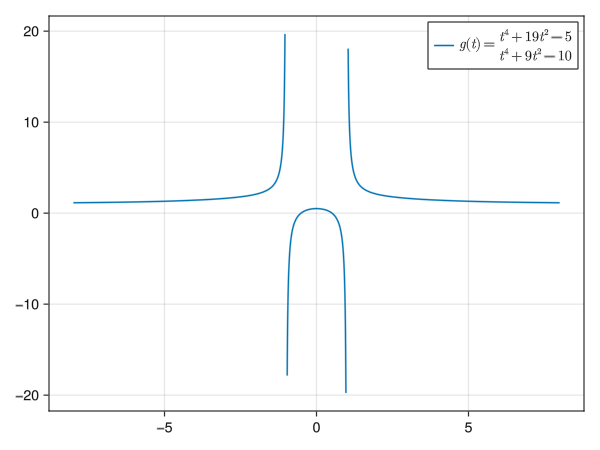
\includegraphics{03-funciones-elementales_files/figure-pdf/cell-22-output-1.png}

\section{Plots}

\begin{Shaded}
\begin{Highlighting}[]
\ImportTok{using} \BuiltInTok{Plots}
\FunctionTok{g}\NormalTok{(t) }\OperatorTok{=}\NormalTok{ (t}\OperatorTok{\^{}}\FloatTok{4}\OperatorTok{+}\FloatTok{19}\NormalTok{t}\OperatorTok{\^{}}\FloatTok{2}\OperatorTok{{-}}\FloatTok{5}\NormalTok{) }\OperatorTok{/}\NormalTok{ (t}\OperatorTok{\^{}}\FloatTok{4}\OperatorTok{+}\FloatTok{9}\NormalTok{t}\OperatorTok{\^{}}\FloatTok{2}\OperatorTok{{-}}\FloatTok{10}\NormalTok{)}
\NormalTok{Plots.}\FunctionTok{plot}\NormalTok{(}\FunctionTok{rangeclamp}\NormalTok{(g), }\OperatorTok{{-}}\FloatTok{8}\NormalTok{, }\FloatTok{8}\NormalTok{, aspect\_ratio}\OperatorTok{=}\FloatTok{1.0}\NormalTok{, ylims}\OperatorTok{=}\NormalTok{(}\OperatorTok{{-}}\FloatTok{5}\NormalTok{,}\FloatTok{5}\NormalTok{) , xticks }\OperatorTok{=}\FunctionTok{Vector}\NormalTok{(}\OperatorTok{{-}}\FloatTok{10}\OperatorTok{:}\FloatTok{10}\NormalTok{), yticks }\OperatorTok{=} \FunctionTok{Vector}\NormalTok{(}\OperatorTok{{-}}\FloatTok{5}\OperatorTok{:}\FloatTok{5}\NormalTok{), label}\OperatorTok{=}\NormalTok{L}\StringTok{"}\SpecialCharTok{$}\NormalTok{g}\StringTok{(t) = }\SpecialCharTok{\textbackslash{}f}\StringTok{rac\{t\^{}4+19t\^{}2{-}5\}\{t\^{}4+9t\^{}2{-}10\}}\SpecialCharTok{$}\StringTok{")}
\end{Highlighting}
\end{Shaded}

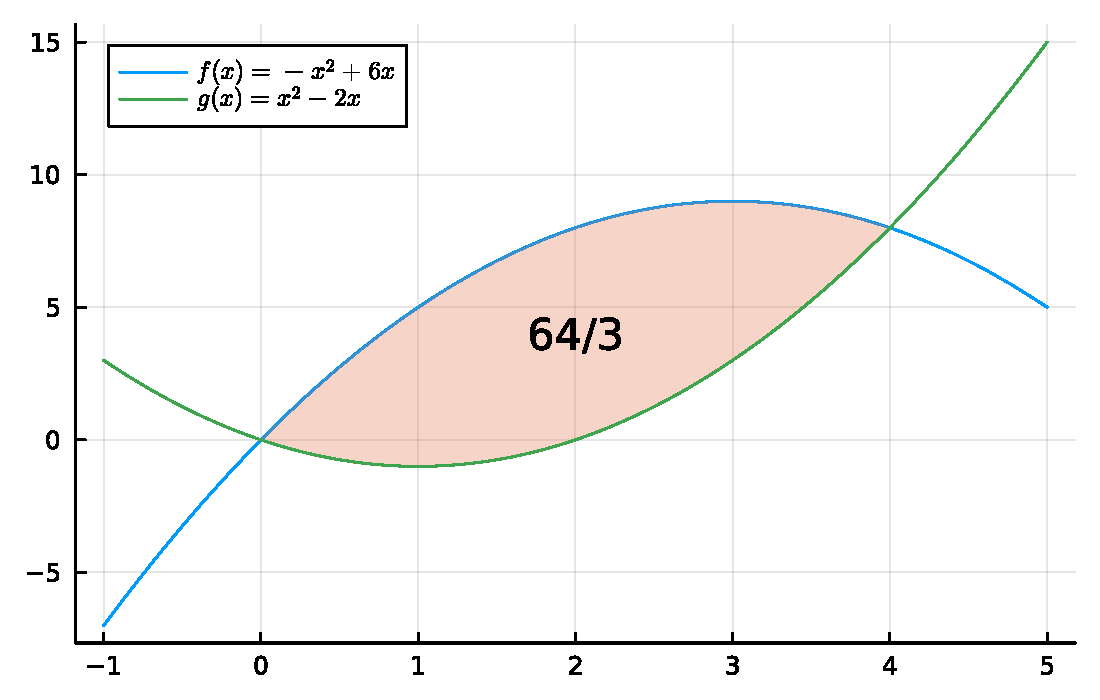
\includegraphics{index_files/mediabag/03-funciones-elementales_files/figure-pdf/cell-23-output-1.pdf}

\end{tcolorbox}

\begin{enumerate}
\def\labelenumi{\alph{enumi}.}
\tightlist
\item
  Dominio. ¿Qué pasa si aplicamos la función a algún valor fuera de su
  dominio?
\end{enumerate}

\begin{tcolorbox}[enhanced jigsaw, bottomtitle=1mm, colframe=quarto-callout-tip-color-frame, bottomrule=.15mm, colback=white, toprule=.15mm, rightrule=.15mm, colbacktitle=quarto-callout-tip-color!10!white, left=2mm, opacitybacktitle=0.6, arc=.35mm, coltitle=black, opacityback=0, breakable, toptitle=1mm, titlerule=0mm, title=\textcolor{quarto-callout-tip-color}{\faLightbulb}\hspace{0.5em}{Solución}, leftrule=.75mm]

\(\operatorname{Dom}(f)=\mathbb{R}\setminus\{-1,1\}\)

\begin{Shaded}
\begin{Highlighting}[]
\FunctionTok{g}\NormalTok{(}\OperatorTok{{-}}\FloatTok{1}\NormalTok{), }\FunctionTok{g}\NormalTok{(}\FloatTok{1}\NormalTok{)}
\end{Highlighting}
\end{Shaded}

\begin{verbatim}
(Inf, Inf)
\end{verbatim}

Como se observa, al aplicar la función a \(-1\) y \(1\) se obtiene
\(\infty\).

\end{tcolorbox}

\begin{enumerate}
\def\labelenumi{\alph{enumi}.}
\setcounter{enumi}{1}
\tightlist
\item
  Imagen
\end{enumerate}

\begin{tcolorbox}[enhanced jigsaw, bottomtitle=1mm, colframe=quarto-callout-tip-color-frame, bottomrule=.15mm, colback=white, toprule=.15mm, rightrule=.15mm, colbacktitle=quarto-callout-tip-color!10!white, left=2mm, opacitybacktitle=0.6, arc=.35mm, coltitle=black, opacityback=0, breakable, toptitle=1mm, titlerule=0mm, title=\textcolor{quarto-callout-tip-color}{\faLightbulb}\hspace{0.5em}{Solución}, leftrule=.75mm]

\(\operatorname{Im}(f)=\mathbb{R}\setminus (0.5,1]\)

\end{tcolorbox}

\begin{enumerate}
\def\labelenumi{\alph{enumi}.}
\setcounter{enumi}{2}
\tightlist
\item
  Asíntotas. Dibujarlas.
\end{enumerate}

\begin{tcolorbox}[enhanced jigsaw, bottomtitle=1mm, colframe=quarto-callout-note-color-frame, bottomrule=.15mm, colback=white, toprule=.15mm, rightrule=.15mm, colbacktitle=quarto-callout-note-color!10!white, left=2mm, opacitybacktitle=0.6, arc=.35mm, coltitle=black, opacityback=0, breakable, toptitle=1mm, titlerule=0mm, title=\textcolor{quarto-callout-note-color}{\faInfo}\hspace{0.5em}{Ayuda}, leftrule=.75mm]

Buscar las asíntotas verticales en los puntos fuera del dominio de la
función.

Para dibujar asíntotas verticales usar la función
\href{https://docs.makie.org/stable/reference/plots/hvlines/index.html}{\texttt{vlines!}}
del paquete \texttt{Makie}, o
\href{https://docs.juliaplots.org/latest/api/\#Plots.vline-Tuple}{\texttt{vline}}
del paquete \texttt{Plots}, y para dibujar las asíntotas horizontales
usar la función
\href{https://docs.makie.org/stable/reference/plots/hvlines/index.html}{\texttt{hlines!}}
del paquete \texttt{Makie}, o
\href{https://docs.juliaplots.org/latest/api/\#Plots.hline-Tuple}{\texttt{hline}}
del paquete \texttt{Plots}.

\end{tcolorbox}

\begin{tcolorbox}[enhanced jigsaw, bottomtitle=1mm, colframe=quarto-callout-tip-color-frame, bottomrule=.15mm, colback=white, toprule=.15mm, rightrule=.15mm, colbacktitle=quarto-callout-tip-color!10!white, left=2mm, opacitybacktitle=0.6, arc=.35mm, coltitle=black, opacityback=0, breakable, toptitle=1mm, titlerule=0mm, title=\textcolor{quarto-callout-tip-color}{\faLightbulb}\hspace{0.5em}{Solución}, leftrule=.75mm]

\section{Makie}

\begin{Shaded}
\begin{Highlighting}[]
\NormalTok{av }\OperatorTok{=}\NormalTok{ Makie.}\FunctionTok{vlines!}\NormalTok{(ax, [}\OperatorTok{{-}}\FloatTok{1}\NormalTok{,}\FloatTok{1}\NormalTok{], color }\OperatorTok{=} \OperatorTok{:}\NormalTok{red)}
\NormalTok{ah }\OperatorTok{=}\NormalTok{ Makie.}\FunctionTok{hlines!}\NormalTok{([}\FloatTok{1}\NormalTok{], color }\OperatorTok{=} \OperatorTok{:}\NormalTok{green)}
\FunctionTok{axislegend}\NormalTok{(ax, [av, ah], [}\StringTok{"Asíntotas verticales"}\NormalTok{, }\StringTok{"Asíntotas Horizontales"}\NormalTok{], position }\OperatorTok{=} \OperatorTok{:}\NormalTok{rb)}
\NormalTok{fig}
\end{Highlighting}
\end{Shaded}

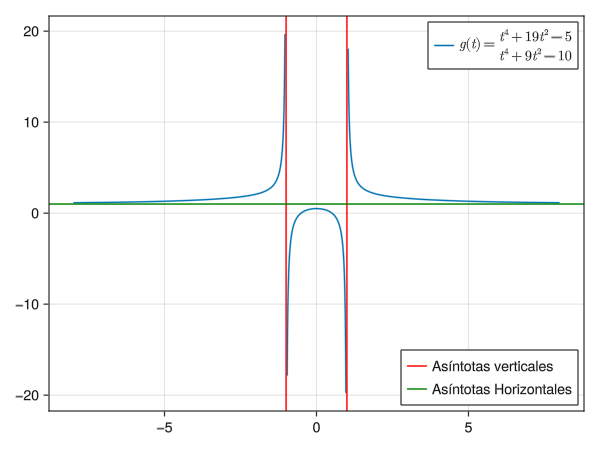
\includegraphics{03-funciones-elementales_files/figure-pdf/cell-25-output-1.png}

\section{Plots}

\begin{Shaded}
\begin{Highlighting}[]
\NormalTok{Plots.}\FunctionTok{vline!}\NormalTok{([}\OperatorTok{{-}}\FloatTok{1}\NormalTok{,}\FloatTok{1}\NormalTok{], label}\OperatorTok{=}\StringTok{"Asíntotas verticales"}\NormalTok{)}
\NormalTok{Plots.}\FunctionTok{hline!}\NormalTok{([}\FloatTok{1}\NormalTok{], label}\OperatorTok{=}\StringTok{"Asíntotas horizontales"}\NormalTok{, legend}\OperatorTok{=:}\NormalTok{bottomright)}
\end{Highlighting}
\end{Shaded}

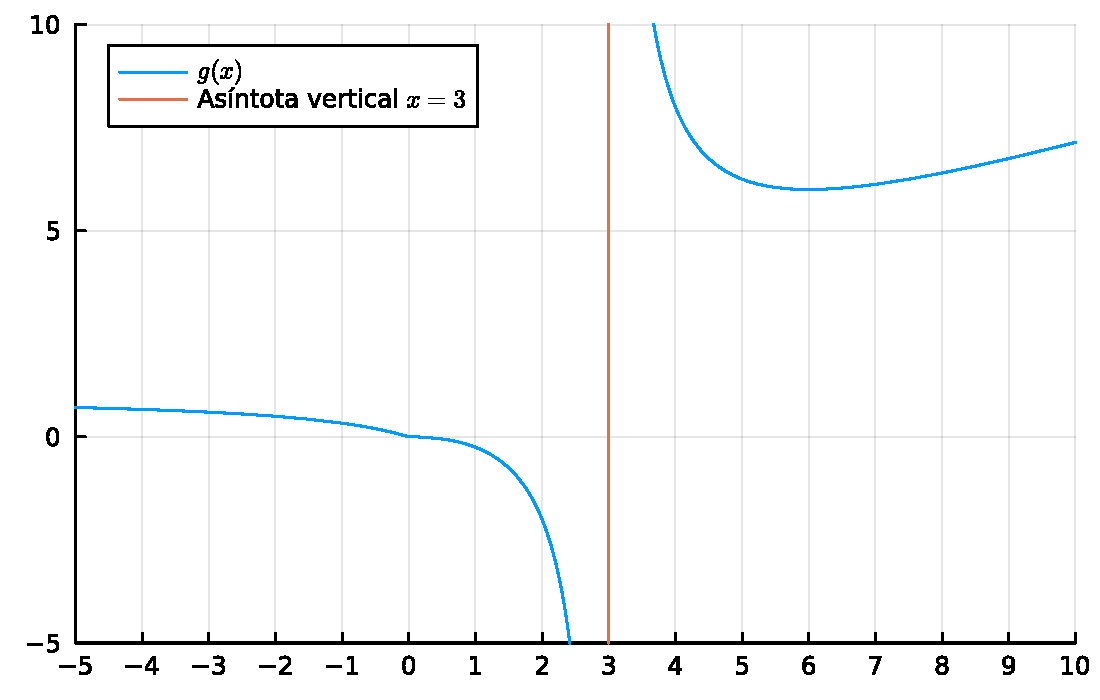
\includegraphics{index_files/mediabag/03-funciones-elementales_files/figure-pdf/cell-26-output-1.pdf}

Asíntotas verticales en \(x=-1\) y \(x=1\).\\
Asíntotas horizontales en \(y=1\).\\
No hay asíntotas oblicuas.

\end{tcolorbox}

\begin{enumerate}
\def\labelenumi{\alph{enumi}.}
\setcounter{enumi}{3}
\tightlist
\item
  Raíces
\end{enumerate}

\begin{tcolorbox}[enhanced jigsaw, bottomtitle=1mm, colframe=quarto-callout-tip-color-frame, bottomrule=.15mm, colback=white, toprule=.15mm, rightrule=.15mm, colbacktitle=quarto-callout-tip-color!10!white, left=2mm, opacitybacktitle=0.6, arc=.35mm, coltitle=black, opacityback=0, breakable, toptitle=1mm, titlerule=0mm, title=\textcolor{quarto-callout-tip-color}{\faLightbulb}\hspace{0.5em}{Solución}, leftrule=.75mm]

Hay dos raíces en \(x=-0.5\) y \(x=0.5\) aproximadamente.

\end{tcolorbox}

\begin{enumerate}
\def\labelenumi{\alph{enumi}.}
\setcounter{enumi}{4}
\tightlist
\item
  Signo
\end{enumerate}

\begin{tcolorbox}[enhanced jigsaw, bottomtitle=1mm, colframe=quarto-callout-tip-color-frame, bottomrule=.15mm, colback=white, toprule=.15mm, rightrule=.15mm, colbacktitle=quarto-callout-tip-color!10!white, left=2mm, opacitybacktitle=0.6, arc=.35mm, coltitle=black, opacityback=0, breakable, toptitle=1mm, titlerule=0mm, title=\textcolor{quarto-callout-tip-color}{\faLightbulb}\hspace{0.5em}{Solución}, leftrule=.75mm]

Intervalos con \(f(x)\) positiva:
\((-\infty,-1)\cup (-0.5,0.5)\cup (1,\infty)\).\\
Intervalos con \(f(x)\) negativa: \((-1,-0.5)\cup (0.5,1)\).

\end{tcolorbox}

\begin{enumerate}
\def\labelenumi{\alph{enumi}.}
\setcounter{enumi}{4}
\tightlist
\item
  Crecimiento
\end{enumerate}

\begin{tcolorbox}[enhanced jigsaw, bottomtitle=1mm, colframe=quarto-callout-tip-color-frame, bottomrule=.15mm, colback=white, toprule=.15mm, rightrule=.15mm, colbacktitle=quarto-callout-tip-color!10!white, left=2mm, opacitybacktitle=0.6, arc=.35mm, coltitle=black, opacityback=0, breakable, toptitle=1mm, titlerule=0mm, title=\textcolor{quarto-callout-tip-color}{\faLightbulb}\hspace{0.5em}{Solución}, leftrule=.75mm]

Intervalos con \(f(x)\) creciente: \((-\infty, -1)\cup (-1,0)\).\\
Intervalos con \(f(x)\) decreciente: \((0,1)\cup (1,\infty)\).

\end{tcolorbox}

\begin{enumerate}
\def\labelenumi{\alph{enumi}.}
\setcounter{enumi}{5}
\tightlist
\item
  Extremos
\end{enumerate}

\begin{tcolorbox}[enhanced jigsaw, bottomtitle=1mm, colframe=quarto-callout-tip-color-frame, bottomrule=.15mm, colback=white, toprule=.15mm, rightrule=.15mm, colbacktitle=quarto-callout-tip-color!10!white, left=2mm, opacitybacktitle=0.6, arc=.35mm, coltitle=black, opacityback=0, breakable, toptitle=1mm, titlerule=0mm, title=\textcolor{quarto-callout-tip-color}{\faLightbulb}\hspace{0.5em}{Solución}, leftrule=.75mm]

Máximo relativo en \(x=0\) y el valor máximo es \(g(0)=0.5\).\\
No hay mínimos relativos.

\end{tcolorbox}

\begin{enumerate}
\def\labelenumi{\alph{enumi}.}
\setcounter{enumi}{6}
\tightlist
\item
  Concavidad
\end{enumerate}

\begin{tcolorbox}[enhanced jigsaw, bottomtitle=1mm, colframe=quarto-callout-tip-color-frame, bottomrule=.15mm, colback=white, toprule=.15mm, rightrule=.15mm, colbacktitle=quarto-callout-tip-color!10!white, left=2mm, opacitybacktitle=0.6, arc=.35mm, coltitle=black, opacityback=0, breakable, toptitle=1mm, titlerule=0mm, title=\textcolor{quarto-callout-tip-color}{\faLightbulb}\hspace{0.5em}{Solución}, leftrule=.75mm]

Intervalos de concavidad hacia arriba:
\((-\infty,-1)\cup (1,\infty)\).\\
Intervalos de concavidad hacia abajo: \((-1,1)\).

\end{tcolorbox}

\begin{enumerate}
\def\labelenumi{\alph{enumi}.}
\setcounter{enumi}{7}
\tightlist
\item
  Puntos de inflexión
\end{enumerate}

\begin{tcolorbox}[enhanced jigsaw, bottomtitle=1mm, colframe=quarto-callout-tip-color-frame, bottomrule=.15mm, colback=white, toprule=.15mm, rightrule=.15mm, colbacktitle=quarto-callout-tip-color!10!white, left=2mm, opacitybacktitle=0.6, arc=.35mm, coltitle=black, opacityback=0, breakable, toptitle=1mm, titlerule=0mm, title=\textcolor{quarto-callout-tip-color}{\faLightbulb}\hspace{0.5em}{Solución}, leftrule=.75mm]

No hay puntos de inflexión.

\end{tcolorbox}

\end{exercise}

\begin{exercise}[]\protect\hypertarget{exr-funciones-exponenciales}{}\label{exr-funciones-exponenciales}

Dibujar la gráficas de las siguientes funciones exponenciales \(2^x\),
\(e^x\), \(0.5^x\), \(0.7^x\) y responder a las siguientes preguntas
comparando las gráficas.

\begin{tcolorbox}[enhanced jigsaw, bottomtitle=1mm, colframe=quarto-callout-tip-color-frame, bottomrule=.15mm, colback=white, toprule=.15mm, rightrule=.15mm, colbacktitle=quarto-callout-tip-color!10!white, left=2mm, opacitybacktitle=0.6, arc=.35mm, coltitle=black, opacityback=0, breakable, toptitle=1mm, titlerule=0mm, title=\textcolor{quarto-callout-tip-color}{\faLightbulb}\hspace{0.5em}{Solución}, leftrule=.75mm]

\section{Makie}

\begin{Shaded}
\begin{Highlighting}[]
\ImportTok{using} \BuiltInTok{GLMakie}
\NormalTok{fig }\OperatorTok{=} \FunctionTok{Figure}\NormalTok{()}
\NormalTok{ax }\OperatorTok{=} \FunctionTok{Axis}\NormalTok{(fig[}\FloatTok{1}\NormalTok{,}\FloatTok{1}\NormalTok{])}
\NormalTok{Makie.}\FunctionTok{lines!}\NormalTok{(ax, }\OperatorTok{{-}}\FloatTok{2}\OperatorTok{..}\FloatTok{2}\NormalTok{, x }\OperatorTok{{-}\textgreater{}} \FloatTok{2}\OperatorTok{\^{}}\NormalTok{x, label}\OperatorTok{=}\NormalTok{L}\StringTok{"}\SpecialCharTok{$}\StringTok{2\^{}}\NormalTok{x}\SpecialCharTok{$}\StringTok{")}
\NormalTok{Makie}\StringTok{.lines!(ax, {-}2..2, exp, label=L"}\OperatorTok{$}\NormalTok{e}\OperatorTok{\^{}}\NormalTok{x}\OperatorTok{$}\StringTok{")}
\NormalTok{Makie.}\FunctionTok{lines!}\NormalTok{(ax, }\OperatorTok{{-}}\FloatTok{2}\OperatorTok{..}\FloatTok{2}\NormalTok{, x }\OperatorTok{{-}\textgreater{}} \FloatTok{0.5}\OperatorTok{\^{}}\NormalTok{x, label}\OperatorTok{=}\NormalTok{L}\StringTok{"}\SpecialCharTok{$}\StringTok{0.5\^{}}\NormalTok{x}\SpecialCharTok{$}\StringTok{")}
\NormalTok{Makie}\StringTok{.lines!(ax, {-}2..2, x {-}\textgreater{} 0.7\^{}x, label=L"}\OperatorTok{$}\FloatTok{0.7}\OperatorTok{\^{}}\NormalTok{x}\OperatorTok{$}\StringTok{")}
\FunctionTok{axislegend}\NormalTok{(position }\OperatorTok{=} \OperatorTok{:}\NormalTok{lt)}
\NormalTok{fig}
\end{Highlighting}
\end{Shaded}

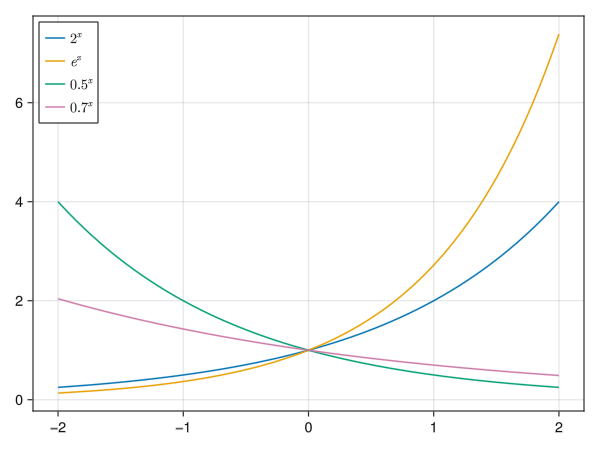
\includegraphics{03-funciones-elementales_files/figure-pdf/cell-27-output-1.png}

\section{Plots}

\begin{Shaded}
\begin{Highlighting}[]
\ImportTok{using} \BuiltInTok{Plots}\NormalTok{, }\BuiltInTok{LaTeXStrings}
\NormalTok{Plots.}\FunctionTok{plot}\NormalTok{(}\FloatTok{2}\OperatorTok{\^{}}\NormalTok{x, }\OperatorTok{{-}}\FloatTok{2}\NormalTok{, }\FloatTok{2}\NormalTok{, label}\OperatorTok{=}\NormalTok{L}\StringTok{"}\SpecialCharTok{$}\StringTok{2\^{}}\NormalTok{x}\SpecialCharTok{$}\StringTok{")}
\NormalTok{Plots}\StringTok{.plot!(exp(x), label=L"}\OperatorTok{$}\NormalTok{e}\OperatorTok{\^{}}\NormalTok{x}\OperatorTok{$}\StringTok{")}
\NormalTok{Plots.}\FunctionTok{plot!}\NormalTok{(}\FloatTok{0.5}\OperatorTok{\^{}}\NormalTok{x, label}\OperatorTok{=}\NormalTok{L}\StringTok{"}\SpecialCharTok{$}\StringTok{2\^{}}\NormalTok{x}\SpecialCharTok{$}\StringTok{")}
\NormalTok{Plots}\StringTok{.plot!(0.7\^{}x, label=L"}\OperatorTok{$}\FloatTok{2}\OperatorTok{\^{}}\NormalTok{x}\OperatorTok{$}\StringTok{")}
\end{Highlighting}
\end{Shaded}

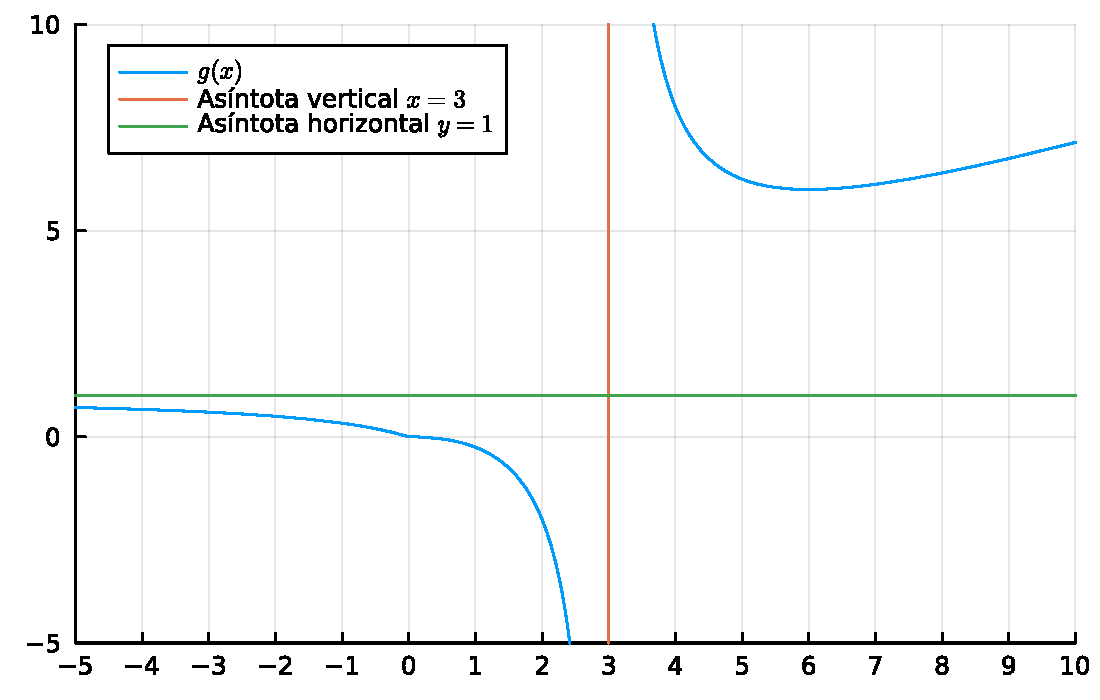
\includegraphics{index_files/mediabag/03-funciones-elementales_files/figure-pdf/cell-28-output-1.pdf}

\end{tcolorbox}

\begin{enumerate}
\def\labelenumi{\alph{enumi}.}
\tightlist
\item
  ¿Cuál es el dominio de una función exponencial?
\end{enumerate}

\begin{tcolorbox}[enhanced jigsaw, bottomtitle=1mm, colframe=quarto-callout-tip-color-frame, bottomrule=.15mm, colback=white, toprule=.15mm, rightrule=.15mm, colbacktitle=quarto-callout-tip-color!10!white, left=2mm, opacitybacktitle=0.6, arc=.35mm, coltitle=black, opacityback=0, breakable, toptitle=1mm, titlerule=0mm, title=\textcolor{quarto-callout-tip-color}{\faLightbulb}\hspace{0.5em}{Solución}, leftrule=.75mm]

\(\mathbb{R}\).

\end{tcolorbox}

\begin{enumerate}
\def\labelenumi{\alph{enumi}.}
\setcounter{enumi}{1}
\tightlist
\item
  ¿Cuál es la imagen de una función exponencial?
\end{enumerate}

\begin{tcolorbox}[enhanced jigsaw, bottomtitle=1mm, colframe=quarto-callout-tip-color-frame, bottomrule=.15mm, colback=white, toprule=.15mm, rightrule=.15mm, colbacktitle=quarto-callout-tip-color!10!white, left=2mm, opacitybacktitle=0.6, arc=.35mm, coltitle=black, opacityback=0, breakable, toptitle=1mm, titlerule=0mm, title=\textcolor{quarto-callout-tip-color}{\faLightbulb}\hspace{0.5em}{Solución}, leftrule=.75mm]

\(\mathbb{R}^+\).

\end{tcolorbox}

\begin{enumerate}
\def\labelenumi{\alph{enumi}.}
\setcounter{enumi}{2}
\tightlist
\item
  ¿Cómo es el crecimiento de una función exponencial?
\end{enumerate}

\begin{tcolorbox}[enhanced jigsaw, bottomtitle=1mm, colframe=quarto-callout-tip-color-frame, bottomrule=.15mm, colback=white, toprule=.15mm, rightrule=.15mm, colbacktitle=quarto-callout-tip-color!10!white, left=2mm, opacitybacktitle=0.6, arc=.35mm, coltitle=black, opacityback=0, breakable, toptitle=1mm, titlerule=0mm, title=\textcolor{quarto-callout-tip-color}{\faLightbulb}\hspace{0.5em}{Solución}, leftrule=.75mm]

\(a^x\) es creciente si \(a>1\) y decreciente si \(0<a<1\).

\end{tcolorbox}

\begin{enumerate}
\def\labelenumi{\alph{enumi}.}
\setcounter{enumi}{3}
\tightlist
\item
  ¿Tienen extremos una función exponencial?
\end{enumerate}

\begin{tcolorbox}[enhanced jigsaw, bottomtitle=1mm, colframe=quarto-callout-tip-color-frame, bottomrule=.15mm, colback=white, toprule=.15mm, rightrule=.15mm, colbacktitle=quarto-callout-tip-color!10!white, left=2mm, opacitybacktitle=0.6, arc=.35mm, coltitle=black, opacityback=0, breakable, toptitle=1mm, titlerule=0mm, title=\textcolor{quarto-callout-tip-color}{\faLightbulb}\hspace{0.5em}{Solución}, leftrule=.75mm]

No

\end{tcolorbox}

\begin{enumerate}
\def\labelenumi{\alph{enumi}.}
\setcounter{enumi}{4}
\tightlist
\item
  ¿Cómo es la curvatura de una función exponencial?
\end{enumerate}

\begin{tcolorbox}[enhanced jigsaw, bottomtitle=1mm, colframe=quarto-callout-tip-color-frame, bottomrule=.15mm, colback=white, toprule=.15mm, rightrule=.15mm, colbacktitle=quarto-callout-tip-color!10!white, left=2mm, opacitybacktitle=0.6, arc=.35mm, coltitle=black, opacityback=0, breakable, toptitle=1mm, titlerule=0mm, title=\textcolor{quarto-callout-tip-color}{\faLightbulb}\hspace{0.5em}{Solución}, leftrule=.75mm]

Es cóncava hacia arriba.

\end{tcolorbox}

\end{exercise}

\begin{exercise}[]\protect\hypertarget{exr-funciones-trigonométricas}{}\label{exr-funciones-trigonométricas}

Dibujar la gráficas de las funciones trigonométricas
\(\operatorname{sen}(x)\), \(\operatorname{sen}(x+2)\),
\(\operatorname{sen}(x)+2\), \(\operatorname{sen}(2x)\) y
\(2\operatorname{sen}(x)\), y completar la siguiente tabla estudiando su
periodo y amplitud.

\begin{longtable}[]{@{}lll@{}}
\toprule\noalign{}
Función & Periodo & Amplitud \\
\midrule\noalign{}
\endhead
\bottomrule\noalign{}
\endlastfoot
\(\operatorname{sen}(x)\) & & \\
\(\operatorname{sen}(x+2)\) & & \\
\(\operatorname{sen}(x)+2\) & & \\
\(\operatorname{sen}(2x)\) & & \\
\(2\operatorname{sen}(x)\) & & \\
\end{longtable}

¿Qué conclusiones sacas?

\begin{tcolorbox}[enhanced jigsaw, bottomtitle=1mm, colframe=quarto-callout-note-color-frame, bottomrule=.15mm, colback=white, toprule=.15mm, rightrule=.15mm, colbacktitle=quarto-callout-note-color!10!white, left=2mm, opacitybacktitle=0.6, arc=.35mm, coltitle=black, opacityback=0, breakable, toptitle=1mm, titlerule=0mm, title=\textcolor{quarto-callout-note-color}{\faInfo}\hspace{0.5em}{Ayuda}, leftrule=.75mm]

El periodo es el mínimo intervalo en el que la gráfica de la función se
repite, y la amplitud es la mitad de la diferencia entre el máximo y el
mínimo de la función.

\end{tcolorbox}

\begin{tcolorbox}[enhanced jigsaw, bottomtitle=1mm, colframe=quarto-callout-tip-color-frame, bottomrule=.15mm, colback=white, toprule=.15mm, rightrule=.15mm, colbacktitle=quarto-callout-tip-color!10!white, left=2mm, opacitybacktitle=0.6, arc=.35mm, coltitle=black, opacityback=0, breakable, toptitle=1mm, titlerule=0mm, title=\textcolor{quarto-callout-tip-color}{\faLightbulb}\hspace{0.5em}{Solución}, leftrule=.75mm]

\section{Makie}

\begin{Shaded}
\begin{Highlighting}[]
\ImportTok{using} \BuiltInTok{GLMakie}
\NormalTok{fig }\OperatorTok{=} \FunctionTok{Figure}\NormalTok{()}
\NormalTok{ax }\OperatorTok{=} \FunctionTok{Axis}\NormalTok{(fig[}\FloatTok{1}\NormalTok{,}\FloatTok{1}\NormalTok{])}
\NormalTok{Makie.}\FunctionTok{lines!}\NormalTok{(ax, }\OperatorTok{{-}}\FloatTok{2}\NormalTok{pi}\OperatorTok{..}\FloatTok{2}\NormalTok{pi, x }\OperatorTok{{-}\textgreater{}} \FunctionTok{sin}\NormalTok{(x}\OperatorTok{+}\FloatTok{2}\NormalTok{), label}\OperatorTok{=}\NormalTok{L}\StringTok{"}\SpecialCharTok{$}\StringTok{\textbackslash{}}\NormalTok{sin}\StringTok{(x+2)}\SpecialCharTok{$}\StringTok{")}
\NormalTok{Makie}\StringTok{.lines!(ax, {-}2pi..2pi, x {-}\textgreater{} sin(x)+2, label=L"}\OperatorTok{$}\FunctionTok{\textbackslash{}sin}\NormalTok{(x)}\OperatorTok{+}\FloatTok{2}\OperatorTok{$}\StringTok{")}
\NormalTok{Makie.}\FunctionTok{lines!}\NormalTok{(ax, }\OperatorTok{{-}}\FloatTok{2}\NormalTok{pi}\OperatorTok{..}\FloatTok{2}\NormalTok{pi, x }\OperatorTok{{-}\textgreater{}} \FunctionTok{sin}\NormalTok{(}\FloatTok{2}\NormalTok{x), label}\OperatorTok{=}\NormalTok{L}\StringTok{"}\SpecialCharTok{$}\StringTok{\textbackslash{}}\NormalTok{sin}\StringTok{(2x)}\SpecialCharTok{$}\StringTok{")}
\NormalTok{Makie}\StringTok{.lines!(ax, {-}2pi..2pi, x {-}\textgreater{} 2sin(x), label=L"}\OperatorTok{$}\FloatTok{2}\FunctionTok{\textbackslash{}sin}\NormalTok{(x)}\OperatorTok{$}\StringTok{")}
\FunctionTok{axislegend}\NormalTok{()}
\NormalTok{fig}
\end{Highlighting}
\end{Shaded}

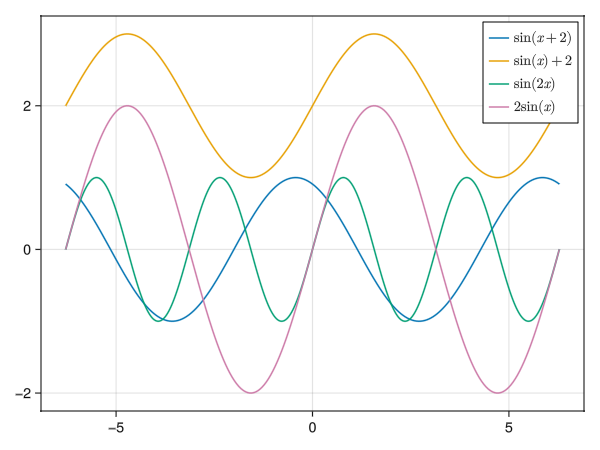
\includegraphics{03-funciones-elementales_files/figure-pdf/cell-29-output-1.png}

\section{Plots}

\begin{Shaded}
\begin{Highlighting}[]
\ImportTok{using} \BuiltInTok{Plots}\NormalTok{, }\BuiltInTok{LaTeXStrings}
\NormalTok{Plots.}\FunctionTok{plot}\NormalTok{(}\FunctionTok{sin}\NormalTok{(x), }\OperatorTok{{-}}\FloatTok{2}\OperatorTok{*}\ConstantTok{pi}\NormalTok{, }\FloatTok{2}\OperatorTok{*}\ConstantTok{pi}\NormalTok{, label}\OperatorTok{=}\NormalTok{L}\StringTok{"}\SpecialCharTok{$}\StringTok{\textbackslash{}}\NormalTok{operatorname}\StringTok{\{sen\}(x)}\SpecialCharTok{$}\StringTok{")}
\NormalTok{Plots}\StringTok{.plot!(sin(x+2), label=L"}\OperatorTok{$}\FunctionTok{\textbackslash{}operatorname}\DataTypeTok{\{sen\}}\NormalTok{(x}\OperatorTok{+}\FloatTok{2}\NormalTok{)}\OperatorTok{$}\StringTok{")}
\NormalTok{Plots.}\FunctionTok{plot!}\NormalTok{(}\FunctionTok{sin}\NormalTok{(x)}\OperatorTok{+}\FloatTok{2}\NormalTok{, label}\OperatorTok{=}\NormalTok{L}\StringTok{"}\SpecialCharTok{$}\StringTok{\textbackslash{}}\NormalTok{operatorname}\StringTok{\{sen\}(x)+2}\SpecialCharTok{$}\StringTok{")}
\NormalTok{Plots}\StringTok{.plot!(sin(2x), label=L"}\OperatorTok{$}\FunctionTok{\textbackslash{}operatorname}\DataTypeTok{\{sen\}}\NormalTok{(}\FloatTok{2}\NormalTok{x)}\OperatorTok{$}\StringTok{")}
\NormalTok{Plots.}\FunctionTok{plot!}\NormalTok{(}\FloatTok{2}\FunctionTok{sin}\NormalTok{(x), label}\OperatorTok{=}\NormalTok{L}\StringTok{"}\SpecialCharTok{$}\StringTok{2\textbackslash{}}\NormalTok{operatorname}\StringTok{\{sen\}(x)}\SpecialCharTok{$}\StringTok{")}
\end{Highlighting}
\end{Shaded}

\includegraphics{index_files/mediabag/03-funciones-elementales_files/figure-pdf/cell-30-output-1.pdf}

\begin{longtable}[]{@{}lll@{}}
\toprule\noalign{}
Función & Periodo & Amplitud \\
\midrule\noalign{}
\endhead
\bottomrule\noalign{}
\endlastfoot
\(\operatorname{sen}(x)\) & \(2\pi\) & 1 \\
\(\operatorname{sen}(x+2)\) & \(2\pi\) & 1 \\
\(\operatorname{sen}(x)+2\) & \(2\pi\) & 1 \\
\(\operatorname{sen}(2x)\) & \(\pi\) & 1 \\
\(2\operatorname{sen}(x)\) & \(2\pi\) & 2 \\
\end{longtable}

Se observa que al sumar una constante a la función seno o a su
argumento, el periodo y la amplitud no cambian. Sin embargo, si se
multiplica por una constante el seno, cambia la amplitud, y si se
multiplica su argumento, cambia el periodo.

\end{tcolorbox}

\end{exercise}

\begin{exercise}[]\protect\hypertarget{exr-funciones-a-trozos}{}\label{exr-funciones-a-trozos}

Dibujar la gráfica de la función a trozos

\[
h(x)=
\begin{cases}
-2x & \mbox{si } x\leq 0;\\
x^2 & \mbox{si } 0< x \leq 2;\\ 
4 & \mbox{si } 2< x
\end{cases}
\]

\begin{tcolorbox}[enhanced jigsaw, bottomtitle=1mm, colframe=quarto-callout-note-color-frame, bottomrule=.15mm, colback=white, toprule=.15mm, rightrule=.15mm, colbacktitle=quarto-callout-note-color!10!white, left=2mm, opacitybacktitle=0.6, arc=.35mm, coltitle=black, opacityback=0, breakable, toptitle=1mm, titlerule=0mm, title=\textcolor{quarto-callout-note-color}{\faInfo}\hspace{0.5em}{Ayuda}, leftrule=.75mm]

Usar el
\href{https://aprendeconalf.es/manual-julia/estructuras-control.html\#operador-condicional}{operador
condicional} anidado.

\end{tcolorbox}

\begin{tcolorbox}[enhanced jigsaw, bottomtitle=1mm, colframe=quarto-callout-tip-color-frame, bottomrule=.15mm, colback=white, toprule=.15mm, rightrule=.15mm, colbacktitle=quarto-callout-tip-color!10!white, left=2mm, opacitybacktitle=0.6, arc=.35mm, coltitle=black, opacityback=0, breakable, toptitle=1mm, titlerule=0mm, title=\textcolor{quarto-callout-tip-color}{\faLightbulb}\hspace{0.5em}{Solución}, leftrule=.75mm]

\section{Makie}

\begin{Shaded}
\begin{Highlighting}[]
\ImportTok{using} \BuiltInTok{GLMakie}
\FunctionTok{h}\NormalTok{(x) }\OperatorTok{=}\NormalTok{ x}\OperatorTok{\textless{}=}\FloatTok{0}\NormalTok{ ? }\OperatorTok{{-}}\FloatTok{2}\NormalTok{x }\OperatorTok{:}\NormalTok{ x}\OperatorTok{\textless{}=}\FloatTok{2}\NormalTok{ ? x}\OperatorTok{\^{}}\FloatTok{2} \OperatorTok{:} \FloatTok{4}
\NormalTok{Makie.}\FunctionTok{lines}\NormalTok{(}\OperatorTok{{-}}\FloatTok{5}\OperatorTok{..}\FloatTok{5}\NormalTok{, h)}
\end{Highlighting}
\end{Shaded}

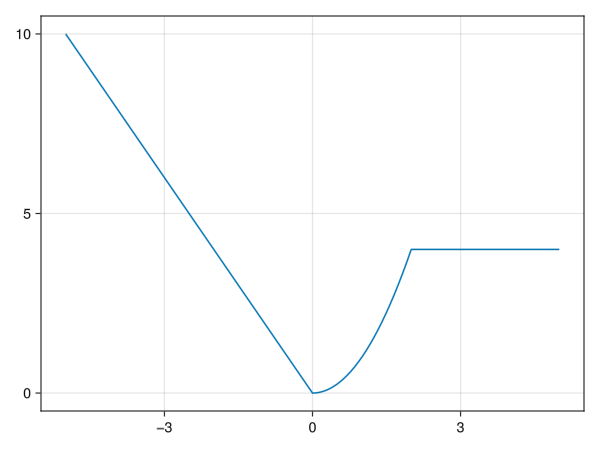
\includegraphics{03-funciones-elementales_files/figure-pdf/cell-31-output-1.png}

\section{Plots}

\begin{Shaded}
\begin{Highlighting}[]
\ImportTok{using} \BuiltInTok{Plots}
\FunctionTok{h}\NormalTok{(x) }\OperatorTok{=}\NormalTok{ x}\OperatorTok{\textless{}=}\FloatTok{0}\NormalTok{ ? }\OperatorTok{{-}}\FloatTok{2}\NormalTok{x }\OperatorTok{:}\NormalTok{ x}\OperatorTok{\textless{}=}\FloatTok{2}\NormalTok{ ? x}\OperatorTok{\^{}}\FloatTok{2} \OperatorTok{:} \FloatTok{4}
\NormalTok{Plots.}\FunctionTok{plot}\NormalTok{(h, legend }\OperatorTok{=} \ConstantTok{false}\NormalTok{)}
\end{Highlighting}
\end{Shaded}

\includegraphics{index_files/mediabag/03-funciones-elementales_files/figure-pdf/cell-32-output-1.pdf}

\end{tcolorbox}

\end{exercise}

\begin{exercise}[]\protect\hypertarget{exr-funciones-parametricas}{}\label{exr-funciones-parametricas}

Una hormiga se mueve sobre el plano real de manera que en cada instante
\(t\) su posición viene dada por las funciones

\[
\begin{cases}
x=\operatorname{sen}(t) \\
y=\operatorname{sen}(2t)
\end{cases}
\]

Dibujar la gráfica de la trayectoria de la hormiga.

\begin{tcolorbox}[enhanced jigsaw, bottomtitle=1mm, colframe=quarto-callout-tip-color-frame, bottomrule=.15mm, colback=white, toprule=.15mm, rightrule=.15mm, colbacktitle=quarto-callout-tip-color!10!white, left=2mm, opacitybacktitle=0.6, arc=.35mm, coltitle=black, opacityback=0, breakable, toptitle=1mm, titlerule=0mm, title=\textcolor{quarto-callout-tip-color}{\faLightbulb}\hspace{0.5em}{Solución}, leftrule=.75mm]

\section{Makie}

\begin{Shaded}
\begin{Highlighting}[]
\ImportTok{using} \BuiltInTok{GLMakie}
\FunctionTok{u1}\NormalTok{(t)}\OperatorTok{=}\FunctionTok{sin}\NormalTok{(t)}
\FunctionTok{v1}\NormalTok{(t)}\OperatorTok{=}\FunctionTok{sin}\NormalTok{(}\FloatTok{2}\NormalTok{t)}
\NormalTok{ts }\OperatorTok{=} \FunctionTok{range}\NormalTok{(}\FloatTok{0}\NormalTok{, }\FloatTok{4}\NormalTok{pi, }\FloatTok{200}\NormalTok{)}
\NormalTok{Makie.}\FunctionTok{lines}\NormalTok{(}\FunctionTok{u1}\NormalTok{.(ts), }\FunctionTok{v1}\NormalTok{.(ts))}
\end{Highlighting}
\end{Shaded}

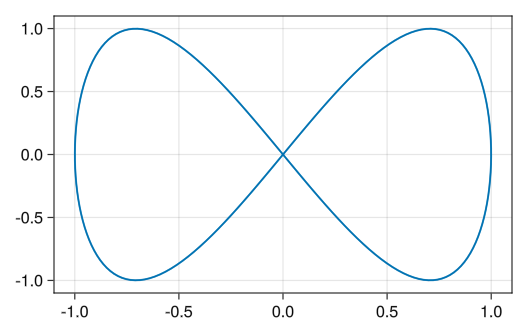
\includegraphics{03-funciones-elementales_files/figure-pdf/cell-33-output-1.png}

\section{Plots}

\begin{Shaded}
\begin{Highlighting}[]
\ImportTok{using} \BuiltInTok{Plots}
\FunctionTok{u1}\NormalTok{(t)}\OperatorTok{=}\FunctionTok{sin}\NormalTok{(t)}
\FunctionTok{v1}\NormalTok{(t)}\OperatorTok{=}\FunctionTok{sin}\NormalTok{(}\FloatTok{2}\NormalTok{t)}
\NormalTok{Plots.}\FunctionTok{plot}\NormalTok{(u1, v1, }\FloatTok{0}\NormalTok{, }\FloatTok{4}\NormalTok{pi, aspect\_ratio}\OperatorTok{=}\FloatTok{1.0}\NormalTok{, legend }\OperatorTok{=} \ConstantTok{false}\NormalTok{)}
\end{Highlighting}
\end{Shaded}

\includegraphics{index_files/mediabag/03-funciones-elementales_files/figure-pdf/cell-34-output-1.pdf}

\end{tcolorbox}

\end{exercise}

\section{Ejercicios propuestos}\label{ejercicios-propuestos-1}

\begin{exercise}[]\protect\hypertarget{exr-dominio-imagen}{}\label{exr-dominio-imagen}

¿Cuáles de las siguientes funciones tienen dominio \(\mathbb{R}\) e
imagen \(\mathbb{R}^+\cup\{0\}\)?

${\quad\Box}$ $$x^4-2x^3+4x$$
${\quad\Box}$ $$2^x$$
${\quad\Box}$ $$1/x^2$$
${\quad\Box}$ $$|x|$$
${\quad\Box}$ $$\sqrt(x)$$
(\emph{Select one or more})

\end{exercise}

\begin{exercise}[]\protect\hypertarget{exr-funciones-logaritmicas}{}\label{exr-funciones-logaritmicas}

Dibujar las gráficas de las funciones logarítmicas \(\ln(x)\),
\(\log_2(x)\) y \(\log_{0.5}(x)\) y contestar a las siguientes
preguntas.

\begin{enumerate}
\def\labelenumi{\alph{enumi}.}
\tightlist
\item
  ¿Cuál es el dominio de una función logarítmica?
\end{enumerate}

${\quad\Box}$ $$\mathbb{R}$$
${\quad\Box}$ $$\mathbb{R}^+\cup \{0\}$$
${\quad\Box}$ $$\mathbb{R}^+$$
${\quad\Box}$ $$\mathbb{R}\setminus\{0\}$$
${\quad\Box}$ Las otras opciones son falsas.

\begin{enumerate}
\def\labelenumi{\alph{enumi}.}
\setcounter{enumi}{1}
\tightlist
\item
  ¿Cuál es la imagen de una función logarítmica?
\end{enumerate}

${\quad\Box}$ $$\mathbb{R}^-$$
${\quad\Box}$ Las otras opciones son falsas.

${\quad\Box}$ $$\mathbb{R}\setminus\{0\}$$
${\quad\Box}$ $$\mathbb{R}^+$$
${\quad\Box}$ $$\mathbb{R}$$

\begin{enumerate}
\def\labelenumi{\alph{enumi}.}
\setcounter{enumi}{2}
\tightlist
\item
  ¿Cómo es el crecimiento la función logarítmica \(\log_a(x)\)?
\end{enumerate}

${\quad\Box}$ Creciente si $0 < a < 1$

${\quad\Box}$ Decreciente si $0 < a <1$

${\quad\Box}$ Creciente si $a<1$

${\quad\Box}$ Creciente si $a>1$

(\emph{Select one or more})

\begin{enumerate}
\def\labelenumi{\alph{enumi}.}
\setcounter{enumi}{3}
\tightlist
\item
  ¿Cómo es la concavidad la función logarítmica \(\log_a(x)\)?
\end{enumerate}

${\quad\Box}$ Cóncava hacia arriba si $a>1$

${\quad\Box}$ Cóncava hacia arriba si $0 < a < 1$

${\quad\Box}$ Cóncava hacia abajo si $0 < a < 1$

${\quad\Box}$ Cóncava hacia abajo si $a<1$

(\emph{Select one or more})

\end{exercise}

\begin{exercise}[]\protect\hypertarget{exr-funciones-trigonométricas}{}\label{exr-funciones-trigonométricas}

¿Cuál es el periodo y la amplitud de la función \(2\cos(x/2)\)?

${\quad\Box}$ π y 2

${\quad\Box}$ 4π y 1

${\quad\Box}$ 2π y 1

${\quad\Box}$ 4π y 2

${\quad\Box}$ 2π y 2

\end{exercise}

\begin{exercise}[]\protect\hypertarget{exr-sucesiones-propuesto-3}{}\label{exr-sucesiones-propuesto-3}

¿Cuál de las gráficas corresponde a la siguiente función paramétrica?

\[
f(t)=
\begin{cases}
\operatorname{sen}(2t)-\cos(t) \\
\operatorname{sen}(t)+\cos(t)
\end{cases}
\]

insert image here

\end{exercise}

\bookmarksetup{startatroot}

\chapter{Límites de funciones
reales}\label{luxedmites-de-funciones-reales}

\section{Ejercicios Resueltos}\label{ejercicios-resueltos-2}

Para la realización de esta práctica se requieren los siguientes
paquetes:

\begin{Shaded}
\begin{Highlighting}[]
\ImportTok{using} \BuiltInTok{SymPy}  \CommentTok{\# Para el cálculo simbólico de límites.}
\ImportTok{using} \BuiltInTok{Plots}  \CommentTok{\# Para el dibujo de gráficas.}
\CommentTok{\#plotlyjs() \# Para obtener gráficos interactivos.}
\ImportTok{using} \BuiltInTok{MTH229} \CommentTok{\# Para restringir la gráfica de una función a su dominio.}
\ImportTok{using} \BuiltInTok{LaTeXStrings}  \CommentTok{\# Para usar código LaTeX en los gráficos.}
\end{Highlighting}
\end{Shaded}

\begin{exercise}[]\protect\hypertarget{exr-tendencia-1}{}\label{exr-tendencia-1}

Sea la función \(f(x)=x^2\).

\begin{enumerate}
\def\labelenumi{\alph{enumi}.}
\item
  Estudiar la tendencia de \(f\) cuando \(x\) se aproxima a \(3\) por la
  derecha, evaluando la función en \(x=3+\frac{1}{10i}\) para
  \(i=1,\ldots,10\).

  \begin{tcolorbox}[enhanced jigsaw, bottomtitle=1mm, colframe=quarto-callout-note-color-frame, bottomrule=.15mm, colback=white, toprule=.15mm, rightrule=.15mm, colbacktitle=quarto-callout-note-color!10!white, left=2mm, opacitybacktitle=0.6, arc=.35mm, coltitle=black, opacityback=0, breakable, toptitle=1mm, titlerule=0mm, title=\textcolor{quarto-callout-note-color}{\faInfo}\hspace{0.5em}{Ayuda}, leftrule=.75mm]

  Definir la función y aplicar la función a los valores de x indicados
  usando
  \href{https://aprendeconalf.es/manual-julia/tipos-datos-compuestos.html\#comprensi\%C3\%B3n-de-arrays}{compresiones
  de arrays}.

  \end{tcolorbox}

  \begin{tcolorbox}[enhanced jigsaw, bottomtitle=1mm, colframe=quarto-callout-tip-color-frame, bottomrule=.15mm, colback=white, toprule=.15mm, rightrule=.15mm, colbacktitle=quarto-callout-tip-color!10!white, left=2mm, opacitybacktitle=0.6, arc=.35mm, coltitle=black, opacityback=0, breakable, toptitle=1mm, titlerule=0mm, title=\textcolor{quarto-callout-tip-color}{\faLightbulb}\hspace{0.5em}{Solución}, leftrule=.75mm]

\begin{Shaded}
\begin{Highlighting}[]
\FunctionTok{f}\NormalTok{(x) }\OperatorTok{=}\NormalTok{ x}\OperatorTok{\^{}}\FloatTok{2}
\NormalTok{a }\OperatorTok{=} \FloatTok{3}
\FunctionTok{print}\NormalTok{([}\FunctionTok{f}\NormalTok{(a}\OperatorTok{+}\FloatTok{1}\OperatorTok{/}\FloatTok{10}\NormalTok{i) for i }\OperatorTok{=} \FloatTok{1}\OperatorTok{:}\FloatTok{10}\NormalTok{])}
\end{Highlighting}
\end{Shaded}

\begin{verbatim}
[9.610000000000001, 9.302499999999998, 9.20111111111111, 9.150625, 9.1204, 9.100277777777777, 9.085918367346938, 9.075156250000001, 9.06679012345679, 9.060099999999998]
\end{verbatim}

  La función tiende a \(9\).

  \end{tcolorbox}
\item
  Estudiar la tendencia de \(f\) cuando \(x\) se aproxima a \(3\) por la
  izquierda, evaluando la función en \(x=3-\frac{1}{10i}\) para
  \(i=1,\ldots, 10\).

  \begin{tcolorbox}[enhanced jigsaw, bottomtitle=1mm, colframe=quarto-callout-tip-color-frame, bottomrule=.15mm, colback=white, toprule=.15mm, rightrule=.15mm, colbacktitle=quarto-callout-tip-color!10!white, left=2mm, opacitybacktitle=0.6, arc=.35mm, coltitle=black, opacityback=0, breakable, toptitle=1mm, titlerule=0mm, title=\textcolor{quarto-callout-tip-color}{\faLightbulb}\hspace{0.5em}{Solución}, leftrule=.75mm]

\begin{Shaded}
\begin{Highlighting}[]
\FunctionTok{print}\NormalTok{([}\FunctionTok{f}\NormalTok{(a}\OperatorTok{{-}}\FloatTok{1}\OperatorTok{/}\FloatTok{10}\NormalTok{i) for i }\OperatorTok{=} \FloatTok{1}\OperatorTok{:}\FloatTok{10}\NormalTok{])}
\end{Highlighting}
\end{Shaded}

\begin{verbatim}
[8.41, 8.7025, 8.801111111111112, 8.850625, 8.8804, 8.900277777777777, 8.914489795918367, 8.925156249999999, 8.933456790123458, 8.940100000000001]
\end{verbatim}

  La función también tiende a 9.

  \end{tcolorbox}
\item
  Dibujar la gráfica de los valores de \(f\) evaluados en los apartados
  anteriores diferenciando la tendencia por la izquierda de la tendencia
  por la derecha.

  \begin{tcolorbox}[enhanced jigsaw, bottomtitle=1mm, colframe=quarto-callout-note-color-frame, bottomrule=.15mm, colback=white, toprule=.15mm, rightrule=.15mm, colbacktitle=quarto-callout-note-color!10!white, left=2mm, opacitybacktitle=0.6, arc=.35mm, coltitle=black, opacityback=0, breakable, toptitle=1mm, titlerule=0mm, title=\textcolor{quarto-callout-note-color}{\faInfo}\hspace{0.5em}{Ayuda}, leftrule=.75mm]

  Definir un vector con los valores de \(x\) y otro con los valores
  correspondientes de \(f(x)\) y usar la función
  \href{https://docs.juliaplots.org/latest/api/\#Plots.scatter-Tuple}{\texttt{scatter}}
  del paquete \texttt{Plots}, pasandole los dos vectores.

  \end{tcolorbox}

  \begin{tcolorbox}[enhanced jigsaw, bottomtitle=1mm, colframe=quarto-callout-tip-color-frame, bottomrule=.15mm, colback=white, toprule=.15mm, rightrule=.15mm, colbacktitle=quarto-callout-tip-color!10!white, left=2mm, opacitybacktitle=0.6, arc=.35mm, coltitle=black, opacityback=0, breakable, toptitle=1mm, titlerule=0mm, title=\textcolor{quarto-callout-tip-color}{\faLightbulb}\hspace{0.5em}{Solución}, leftrule=.75mm]

\begin{Shaded}
\begin{Highlighting}[]
\NormalTok{xd }\OperatorTok{=}\NormalTok{ [a}\OperatorTok{+}\FloatTok{1}\OperatorTok{/}\FloatTok{10}\NormalTok{i for i}\OperatorTok{=}\FloatTok{1}\OperatorTok{:}\FloatTok{10}\NormalTok{]}
\FunctionTok{scatter}\NormalTok{(xd, }\FunctionTok{f}\NormalTok{.(xd), label}\OperatorTok{=}\StringTok{"Aproximación por la derecha"}\NormalTok{)}
\NormalTok{xi }\OperatorTok{=}\NormalTok{ [a}\OperatorTok{{-}}\FloatTok{1}\OperatorTok{/}\FloatTok{10}\NormalTok{i for i}\OperatorTok{=}\FloatTok{1}\OperatorTok{:}\FloatTok{10}\NormalTok{]}
\FunctionTok{scatter!}\NormalTok{(xi, }\FunctionTok{f}\NormalTok{.(xi), label}\OperatorTok{=}\StringTok{"Aproximación por la izquierda"}\NormalTok{, legend}\OperatorTok{=:}\NormalTok{topleft)}
\end{Highlighting}
\end{Shaded}

  \includegraphics{index_files/mediabag/04-limites_files/figure-pdf/cell-5-output-1.pdf}

  \end{tcolorbox}
\item
  Calcular el límite por la izquierda y por la derecha de \(f\) en
  \(x=3\).

  \begin{tcolorbox}[enhanced jigsaw, bottomtitle=1mm, colframe=quarto-callout-note-color-frame, bottomrule=.15mm, colback=white, toprule=.15mm, rightrule=.15mm, colbacktitle=quarto-callout-note-color!10!white, left=2mm, opacitybacktitle=0.6, arc=.35mm, coltitle=black, opacityback=0, breakable, toptitle=1mm, titlerule=0mm, title=\textcolor{quarto-callout-note-color}{\faInfo}\hspace{0.5em}{Ayuda}, leftrule=.75mm]

  Declarar la variable simbólica \texttt{x} con \texttt{@syms}
  imponiento la restricción \texttt{real=true}, definir la función y
  usar la función
  \href{https://docs.juliahub.com/SymPy/KzewI/1.0.31/Tutorial/calculus/\#Limits-1}{\texttt{limit}}
  del paquete \texttt{SymPy} para calcular los límites laterales de la
  función. Para el límite por la izquierda indicar el parámetro
  \texttt{dir="-"} y para el límite por la derecha \texttt{dir="+"}.

  \end{tcolorbox}

  \begin{tcolorbox}[enhanced jigsaw, bottomtitle=1mm, colframe=quarto-callout-tip-color-frame, bottomrule=.15mm, colback=white, toprule=.15mm, rightrule=.15mm, colbacktitle=quarto-callout-tip-color!10!white, left=2mm, opacitybacktitle=0.6, arc=.35mm, coltitle=black, opacityback=0, breakable, toptitle=1mm, titlerule=0mm, title=\textcolor{quarto-callout-tip-color}{\faLightbulb}\hspace{0.5em}{Solución}, leftrule=.75mm]

\begin{Shaded}
\begin{Highlighting}[]
\PreprocessorTok{@syms}\NormalTok{ x}\OperatorTok{::}\DataTypeTok{real}
\NormalTok{li }\OperatorTok{=} \FunctionTok{limit}\NormalTok{(}\FunctionTok{f}\NormalTok{(x), x}\OperatorTok{=\textgreater{}}\FloatTok{3}\NormalTok{, dir}\OperatorTok{=}\StringTok{"{-}"}\NormalTok{)}
\FunctionTok{println}\NormalTok{(}\StringTok{"Límite por la izquierda: "}\NormalTok{, li)}
\NormalTok{ld }\OperatorTok{=} \FunctionTok{limit}\NormalTok{(}\FunctionTok{f}\NormalTok{(x), x}\OperatorTok{=\textgreater{}}\FloatTok{3}\NormalTok{, dir}\OperatorTok{=}\StringTok{"+"}\NormalTok{)}
\FunctionTok{println}\NormalTok{(}\StringTok{"Límite por la derecha: "}\NormalTok{, ld)}
\end{Highlighting}
\end{Shaded}

\begin{verbatim}
Límite por la izquierda: 9
Límite por la derecha: 9
\end{verbatim}

  \end{tcolorbox}
\end{enumerate}

\end{exercise}

\begin{exercise}[]\protect\hypertarget{exr-tendencia-2}{}\label{exr-tendencia-2}

Sea la función \(g(x)=(1+x)^{1/x}\).

\begin{enumerate}
\def\labelenumi{\alph{enumi}.}
\item
  Estudiar la tendencia de \(g\) cuando \(x\) se aproxima a \(0\) por la
  derecha, evaluando la función en \(x=\frac{1}{10^i}\) para
  \(i=1,\ldots,10\).

  \begin{tcolorbox}[enhanced jigsaw, bottomtitle=1mm, colframe=quarto-callout-tip-color-frame, bottomrule=.15mm, colback=white, toprule=.15mm, rightrule=.15mm, colbacktitle=quarto-callout-tip-color!10!white, left=2mm, opacitybacktitle=0.6, arc=.35mm, coltitle=black, opacityback=0, breakable, toptitle=1mm, titlerule=0mm, title=\textcolor{quarto-callout-tip-color}{\faLightbulb}\hspace{0.5em}{Solución}, leftrule=.75mm]

\begin{Shaded}
\begin{Highlighting}[]
\FunctionTok{g}\NormalTok{(x) }\OperatorTok{=}\NormalTok{ (}\FloatTok{1}\OperatorTok{+}\NormalTok{x)}\OperatorTok{\^{}}\NormalTok{(}\FloatTok{1}\OperatorTok{/}\NormalTok{x)}
\NormalTok{a }\OperatorTok{=} \FloatTok{0}
\FunctionTok{print}\NormalTok{([}\FunctionTok{g}\NormalTok{(a}\OperatorTok{+}\FloatTok{1}\OperatorTok{/}\FloatTok{10}\OperatorTok{\^{}}\NormalTok{i) for i }\OperatorTok{=} \FloatTok{1}\OperatorTok{:}\FloatTok{10}\NormalTok{])}
\end{Highlighting}
\end{Shaded}

\begin{verbatim}
[2.5937424601000023, 2.7048138294215285, 2.7169239322355936, 2.7181459268249255, 2.718268237192297, 2.7182804690957534, 2.7182816941320818, 2.7182817983473577, 2.71828205201156, 2.7182820532347876]
\end{verbatim}

  La función tiende a \(e\).

  \end{tcolorbox}
\item
  Estudiar la tendencia de \(g\) cuando \(x\) se aproxima a \(0\) por la
  izquierda, evaluando la función en \(x=-\frac{1}{10^i}\) para
  \(i=1,\ldots, 10\).

  \begin{tcolorbox}[enhanced jigsaw, bottomtitle=1mm, colframe=quarto-callout-tip-color-frame, bottomrule=.15mm, colback=white, toprule=.15mm, rightrule=.15mm, colbacktitle=quarto-callout-tip-color!10!white, left=2mm, opacitybacktitle=0.6, arc=.35mm, coltitle=black, opacityback=0, breakable, toptitle=1mm, titlerule=0mm, title=\textcolor{quarto-callout-tip-color}{\faLightbulb}\hspace{0.5em}{Solución}, leftrule=.75mm]

\begin{Shaded}
\begin{Highlighting}[]
\FunctionTok{print}\NormalTok{([}\FunctionTok{g}\NormalTok{(a}\OperatorTok{{-}}\FloatTok{1}\OperatorTok{/}\FloatTok{10}\OperatorTok{\^{}}\NormalTok{i) for i }\OperatorTok{=} \FloatTok{1}\OperatorTok{:}\FloatTok{10}\NormalTok{])}
\end{Highlighting}
\end{Shaded}

\begin{verbatim}
[2.867971990792441, 2.7319990264290284, 2.719642216442853, 2.71841775501015, 2.718295419980405, 2.7182831876793716, 2.7182819629423656, 2.7182818557091664, 2.7182817529399266, 2.7182820535066154]
\end{verbatim}

  La función también tiende a e.

  \end{tcolorbox}
\item
  Calcular el límite por la izquierda y por la derecha de \(g\) en
  \(x=0\).

  \begin{tcolorbox}[enhanced jigsaw, bottomtitle=1mm, colframe=quarto-callout-tip-color-frame, bottomrule=.15mm, colback=white, toprule=.15mm, rightrule=.15mm, colbacktitle=quarto-callout-tip-color!10!white, left=2mm, opacitybacktitle=0.6, arc=.35mm, coltitle=black, opacityback=0, breakable, toptitle=1mm, titlerule=0mm, title=\textcolor{quarto-callout-tip-color}{\faLightbulb}\hspace{0.5em}{Solución}, leftrule=.75mm]

\begin{Shaded}
\begin{Highlighting}[]
\PreprocessorTok{@syms}\NormalTok{ x}\OperatorTok{::}\DataTypeTok{real}
\NormalTok{li }\OperatorTok{=} \FunctionTok{limit}\NormalTok{(}\FunctionTok{g}\NormalTok{(x), x}\OperatorTok{=\textgreater{}}\FloatTok{0}\NormalTok{, dir}\OperatorTok{=}\StringTok{"{-}"}\NormalTok{)}
\FunctionTok{println}\NormalTok{(}\StringTok{"Límite por la izquierda: "}\NormalTok{, li)}
\NormalTok{ld }\OperatorTok{=} \FunctionTok{limit}\NormalTok{(}\FunctionTok{g}\NormalTok{(x), x}\OperatorTok{=\textgreater{}}\FloatTok{0}\NormalTok{, dir}\OperatorTok{=}\StringTok{"+"}\NormalTok{)}
\FunctionTok{println}\NormalTok{(}\StringTok{"Límite por la derecha: "}\NormalTok{, ld)}
\end{Highlighting}
\end{Shaded}

\begin{verbatim}
Límite por la izquierda: E
Límite por la derecha: E
\end{verbatim}

  \end{tcolorbox}
\end{enumerate}

\end{exercise}

\begin{exercise}[]\protect\hypertarget{exr-limites-laterales}{}\label{exr-limites-laterales}

Considérese la función \[
f(x)=\left( 1+\frac{2}{x}\right) ^{x/2}.
\]

\begin{enumerate}
\def\labelenumi{\alph{enumi}.}
\item
  Dibujar su gráfica, y a la vista de misma conjeturar el resultado de
  los siguientes límites:

  \begin{itemize}
  \tightlist
  \item
    \(\lim_{x\rightarrow -2^-} f(x)\)
  \item
    \(\lim_{x\rightarrow -2^+} f(x)\)
  \item
    \(\lim_{x\rightarrow -\infty} f(x)\)
  \item
    \(\lim_{x\rightarrow +\infty} f(x)\)
  \item
    \(\lim_{x\rightarrow 2} f(x)\)
  \item
    \(\lim_{x\rightarrow 0} f(x)\)
  \end{itemize}

  \begin{tcolorbox}[enhanced jigsaw, bottomtitle=1mm, colframe=quarto-callout-note-color-frame, bottomrule=.15mm, colback=white, toprule=.15mm, rightrule=.15mm, colbacktitle=quarto-callout-note-color!10!white, left=2mm, opacitybacktitle=0.6, arc=.35mm, coltitle=black, opacityback=0, breakable, toptitle=1mm, titlerule=0mm, title=\textcolor{quarto-callout-note-color}{\faInfo}\hspace{0.5em}{Ayuda}, leftrule=.75mm]

  Utilizar la función
  \href{https://aprendeconalf.es/manual-julia/graficos.html\#gr\%C3\%A1fica-de-una-funci\%C3\%B3n-de-una-variable}{\texttt{plot!}}
  del paquete \texttt{Plots}. Usar los parámetros \texttt{xlims=(a,b)}
  para restringir la región de dibujo al intervalo \((a,b)\) del eje
  \(x\), y \texttt{ylims=(c,d)} para restringir la región de dibujo al
  intervalo \((c,d)\) del eje \(y\).

  \end{tcolorbox}

  \begin{tcolorbox}[enhanced jigsaw, bottomtitle=1mm, colframe=quarto-callout-tip-color-frame, bottomrule=.15mm, colback=white, toprule=.15mm, rightrule=.15mm, colbacktitle=quarto-callout-tip-color!10!white, left=2mm, opacitybacktitle=0.6, arc=.35mm, coltitle=black, opacityback=0, breakable, toptitle=1mm, titlerule=0mm, title=\textcolor{quarto-callout-tip-color}{\faLightbulb}\hspace{0.5em}{Solución}, leftrule=.75mm]

\begin{Shaded}
\begin{Highlighting}[]
\ImportTok{using} \BuiltInTok{Plots}
\FunctionTok{f}\NormalTok{(x) }\OperatorTok{=}\NormalTok{ (}\FloatTok{1}\OperatorTok{+}\FloatTok{2}\OperatorTok{/}\NormalTok{x)}\OperatorTok{\^{}}\NormalTok{(x}\OperatorTok{/}\FloatTok{2}\NormalTok{)}
\FunctionTok{plot}\NormalTok{(f, xlims}\OperatorTok{=}\NormalTok{(}\OperatorTok{{-}}\FloatTok{10}\NormalTok{,}\FloatTok{10}\NormalTok{), ylims}\OperatorTok{=}\NormalTok{(}\FloatTok{0}\NormalTok{,}\FloatTok{6}\NormalTok{))}
\end{Highlighting}
\end{Shaded}

  \includegraphics{index_files/mediabag/04-limites_files/figure-pdf/cell-10-output-1.pdf}

  A la vista de la gráfica, se puede concluir que

  \begin{enumerate}
  \def\labelenumii{\roman{enumii}.}
  \tightlist
  \item
    \(\lim_{x\rightarrow -2^-} f(x) = -\infty.\)
  \item
    \(\lim_{x\rightarrow -2^+} f(x)\) no existe.
  \item
    \(\lim_{x\rightarrow -\infty} f(x)\approx 2.7.\)
  \item
    \(\lim_{x\rightarrow +\infty} f(x) \approx 2.7.\)
  \item
    \(\lim_{x\rightarrow 2} f(x) = 2.\)
  \item
    \(\lim_{x\rightarrow 0} f(x)\) no existe.
  \end{enumerate}

  \end{tcolorbox}
\item
  Calcular los límites anteriores. ¿Coinciden los resultados con los
  conjeturados?

  \begin{tcolorbox}[enhanced jigsaw, bottomtitle=1mm, colframe=quarto-callout-tip-color-frame, bottomrule=.15mm, colback=white, toprule=.15mm, rightrule=.15mm, colbacktitle=quarto-callout-tip-color!10!white, left=2mm, opacitybacktitle=0.6, arc=.35mm, coltitle=black, opacityback=0, breakable, toptitle=1mm, titlerule=0mm, title=\textcolor{quarto-callout-tip-color}{\faLightbulb}\hspace{0.5em}{Solución}, leftrule=.75mm]

\begin{Shaded}
\begin{Highlighting}[]
\ImportTok{using} \BuiltInTok{SymPy}
\PreprocessorTok{@syms}\NormalTok{ x}\OperatorTok{::}\DataTypeTok{real}
\FunctionTok{println}\NormalTok{(}\StringTok{"Límite por la izquieda en {-}2: "}\NormalTok{, }\FunctionTok{limit}\NormalTok{(}\FunctionTok{f}\NormalTok{(x), x}\OperatorTok{=\textgreater{}{-}}\FloatTok{2}\NormalTok{, dir}\OperatorTok{=}\StringTok{"{-}"}\NormalTok{))}
\FunctionTok{println}\NormalTok{(}\StringTok{"Límite por la derecha en {-}2: "}\NormalTok{, }\FunctionTok{limit}\NormalTok{(}\FunctionTok{f}\NormalTok{(x), x}\OperatorTok{=\textgreater{}{-}}\FloatTok{2}\NormalTok{, dir}\OperatorTok{=}\StringTok{"+"}\NormalTok{))}
\FunctionTok{println}\NormalTok{(}\StringTok{"Límite en {-}∞: "}\NormalTok{, }\FunctionTok{limit}\NormalTok{(}\FunctionTok{f}\NormalTok{(x), x}\OperatorTok{=\textgreater{}{-}}\NormalTok{oo))}
\FunctionTok{println}\NormalTok{(}\StringTok{"Límite en ∞: "}\NormalTok{, }\FunctionTok{limit}\NormalTok{(}\FunctionTok{f}\NormalTok{(x), x}\OperatorTok{=\textgreater{}}\NormalTok{oo))}
\FunctionTok{println}\NormalTok{(}\StringTok{"Límite en 2: "}\NormalTok{, }\FunctionTok{limit}\NormalTok{(}\FunctionTok{f}\NormalTok{(x), x}\OperatorTok{=\textgreater{}}\FloatTok{2}\NormalTok{))}
\FunctionTok{println}\NormalTok{(}\StringTok{"Límite en 0: "}\NormalTok{, }\FunctionTok{limit}\NormalTok{(}\FunctionTok{f}\NormalTok{(x), x}\OperatorTok{=\textgreater{}}\FloatTok{0}\NormalTok{))}
\end{Highlighting}
\end{Shaded}

\begin{verbatim}
Límite por la izquieda en -2: oo
Límite por la derecha en -2: -oo
Límite en -∞: E
Límite en ∞: E
Límite en 2: 2
Límite en 0: 1
\end{verbatim}

  \begin{tcolorbox}[enhanced jigsaw, bottomtitle=1mm, colframe=quarto-callout-caution-color-frame, bottomrule=.15mm, colback=white, toprule=.15mm, rightrule=.15mm, colbacktitle=quarto-callout-caution-color!10!white, left=2mm, opacitybacktitle=0.6, arc=.35mm, coltitle=black, opacityback=0, breakable, toptitle=1mm, titlerule=0mm, title=\textcolor{quarto-callout-caution-color}{\faFire}\hspace{0.5em}{Precaución}, leftrule=.75mm]

  Aunque Julia calcula el límite en \(-2\) por la derecha y el límite en
  \(0\), a la vista de la gráfica, estos límites en realidad no existen,
  ya que la función no está definida en el intervalo de \([-2,0]\).

  \end{tcolorbox}

  \end{tcolorbox}
\end{enumerate}

\end{exercise}

\begin{exercise}[]\protect\hypertarget{exr-limites-raros}{}\label{exr-limites-raros}

Calcular los siguientes límites

\begin{enumerate}
\def\labelenumi{\alph{enumi}.}
\item
  \(\lim_{x\to 0} \operatorname{sen}\left(\frac{1}{x}\right)\)

  \begin{tcolorbox}[enhanced jigsaw, bottomtitle=1mm, colframe=quarto-callout-tip-color-frame, bottomrule=.15mm, colback=white, toprule=.15mm, rightrule=.15mm, colbacktitle=quarto-callout-tip-color!10!white, left=2mm, opacitybacktitle=0.6, arc=.35mm, coltitle=black, opacityback=0, breakable, toptitle=1mm, titlerule=0mm, title=\textcolor{quarto-callout-tip-color}{\faLightbulb}\hspace{0.5em}{Solución}, leftrule=.75mm]

\begin{Shaded}
\begin{Highlighting}[]
\ImportTok{using} \BuiltInTok{SymPy}
\PreprocessorTok{@syms}\NormalTok{ x}\OperatorTok{::}\DataTypeTok{real}
\FunctionTok{limit}\NormalTok{(}\FunctionTok{sin}\NormalTok{(}\FloatTok{1}\OperatorTok{/}\NormalTok{x), x}\OperatorTok{=\textgreater{}}\FloatTok{0}\NormalTok{)}
\end{Highlighting}
\end{Shaded}

  $\left\langle -1, 1\right\rangle$

  Como no se obtiene un valor concreto, sino un rango de valores, el
  límite no existe.

  \end{tcolorbox}
\item
  \(\lim_{x\to 0} x\operatorname{sen}\left(\frac{1}{x}\right)\)

  \begin{tcolorbox}[enhanced jigsaw, bottomtitle=1mm, colframe=quarto-callout-tip-color-frame, bottomrule=.15mm, colback=white, toprule=.15mm, rightrule=.15mm, colbacktitle=quarto-callout-tip-color!10!white, left=2mm, opacitybacktitle=0.6, arc=.35mm, coltitle=black, opacityback=0, breakable, toptitle=1mm, titlerule=0mm, title=\textcolor{quarto-callout-tip-color}{\faLightbulb}\hspace{0.5em}{Solución}, leftrule=.75mm]

\begin{Shaded}
\begin{Highlighting}[]
\FunctionTok{limit}\NormalTok{(}\FunctionTok{x*sin}\NormalTok{(}\FloatTok{1}\OperatorTok{/}\NormalTok{x), x}\OperatorTok{=\textgreater{}}\FloatTok{0}\NormalTok{)}
\end{Highlighting}
\end{Shaded}

  $0$

  \end{tcolorbox}
\item
  \(\lim_{x\to \infty} e^{-x}\operatorname{sen}(x)\)

  \begin{tcolorbox}[enhanced jigsaw, bottomtitle=1mm, colframe=quarto-callout-tip-color-frame, bottomrule=.15mm, colback=white, toprule=.15mm, rightrule=.15mm, colbacktitle=quarto-callout-tip-color!10!white, left=2mm, opacitybacktitle=0.6, arc=.35mm, coltitle=black, opacityback=0, breakable, toptitle=1mm, titlerule=0mm, title=\textcolor{quarto-callout-tip-color}{\faLightbulb}\hspace{0.5em}{Solución}, leftrule=.75mm]

\begin{Shaded}
\begin{Highlighting}[]
\FunctionTok{limit}\NormalTok{(}\ConstantTok{ℯ}\OperatorTok{\^{}}\NormalTok{(}\OperatorTok{{-}}\NormalTok{x)}\FunctionTok{*sin}\NormalTok{(x), x}\OperatorTok{=\textgreater{}}\NormalTok{oo)}
\end{Highlighting}
\end{Shaded}

  $0$

  \end{tcolorbox}
\item
  \(\lim_{x\to a} \frac{\operatorname{sen}(x)-\operatorname{sen}(a)}{x-a}\)

  \begin{tcolorbox}[enhanced jigsaw, bottomtitle=1mm, colframe=quarto-callout-tip-color-frame, bottomrule=.15mm, colback=white, toprule=.15mm, rightrule=.15mm, colbacktitle=quarto-callout-tip-color!10!white, left=2mm, opacitybacktitle=0.6, arc=.35mm, coltitle=black, opacityback=0, breakable, toptitle=1mm, titlerule=0mm, title=\textcolor{quarto-callout-tip-color}{\faLightbulb}\hspace{0.5em}{Solución}, leftrule=.75mm]

\begin{Shaded}
\begin{Highlighting}[]
\PreprocessorTok{@syms}\NormalTok{ a}\OperatorTok{::}\DataTypeTok{real}
\FunctionTok{limit}\NormalTok{((}\FunctionTok{sin}\NormalTok{(x)}\FunctionTok{{-}sin}\NormalTok{(a))}\OperatorTok{/}\NormalTok{(x}\OperatorTok{{-}}\NormalTok{a), x}\OperatorTok{=\textgreater{}}\NormalTok{a)}
\end{Highlighting}
\end{Shaded}

  $\cos{\left(a \right)}$

  \end{tcolorbox}
\end{enumerate}

\end{exercise}

\begin{exercise}[]\protect\hypertarget{exr-indeterminaciones}{}\label{exr-indeterminaciones}

Calcular el valor de las siguientes funciones en los puntos dados y su
límite. Corroborar los límites obtenidos gráficamente.

\begin{enumerate}
\def\labelenumi{\alph{enumi}.}
\item
  \(f(x)=\frac{\operatorname{sen}(x)}{x}\) en \(x=0\).

  \begin{tcolorbox}[enhanced jigsaw, bottomtitle=1mm, colframe=quarto-callout-tip-color-frame, bottomrule=.15mm, colback=white, toprule=.15mm, rightrule=.15mm, colbacktitle=quarto-callout-tip-color!10!white, left=2mm, opacitybacktitle=0.6, arc=.35mm, coltitle=black, opacityback=0, breakable, toptitle=1mm, titlerule=0mm, title=\textcolor{quarto-callout-tip-color}{\faLightbulb}\hspace{0.5em}{Solución}, leftrule=.75mm]

  La función \(f\) no está definida en \(x=0\) de manera que al
  evaluarla en \(0\) obtenemos un valor indeterminado.

\begin{Shaded}
\begin{Highlighting}[]
\FunctionTok{f}\NormalTok{(x)}\OperatorTok{=}\FunctionTok{sin}\NormalTok{(x)}\OperatorTok{/}\NormalTok{x}
\FunctionTok{f}\NormalTok{(}\FloatTok{0}\NormalTok{)}
\end{Highlighting}
\end{Shaded}

\begin{verbatim}
NaN
\end{verbatim}

  Ahora calculamos el límite de \(f\) en \(0\).

\begin{Shaded}
\begin{Highlighting}[]
\PreprocessorTok{@syms}\NormalTok{ x}\OperatorTok{::}\DataTypeTok{real}
\FunctionTok{f}\NormalTok{(x)}\OperatorTok{=}\FunctionTok{sin}\NormalTok{(x)}\OperatorTok{/}\NormalTok{x}
\FunctionTok{limit}\NormalTok{(}\FunctionTok{f}\NormalTok{(x), x}\OperatorTok{=\textgreater{}}\FloatTok{0}\NormalTok{)}
\end{Highlighting}
\end{Shaded}

  $1$

  Para corroborar el límite dibujamos la gráfica de \(f\) en un entorno
  de \(0\).

\begin{Shaded}
\begin{Highlighting}[]
\ImportTok{using} \BuiltInTok{Plots}
\FunctionTok{plot}\NormalTok{(f)}
\end{Highlighting}
\end{Shaded}

  \includegraphics{index_files/mediabag/04-limites_files/figure-pdf/cell-18-output-1.pdf}

  \end{tcolorbox}
\item
  \(g(x)=\frac{\cos(x)}{x-\pi/2}\) en \(x=\pi/2\).

  \begin{tcolorbox}[enhanced jigsaw, bottomtitle=1mm, colframe=quarto-callout-tip-color-frame, bottomrule=.15mm, colback=white, toprule=.15mm, rightrule=.15mm, colbacktitle=quarto-callout-tip-color!10!white, left=2mm, opacitybacktitle=0.6, arc=.35mm, coltitle=black, opacityback=0, breakable, toptitle=1mm, titlerule=0mm, title=\textcolor{quarto-callout-tip-color}{\faLightbulb}\hspace{0.5em}{Solución}, leftrule=.75mm]

  La función \(f\) no está definida en \(x=0\) de manera que al
  evaluarla en \(0\) obtenemos un valor indeterminado.

\begin{Shaded}
\begin{Highlighting}[]
\FunctionTok{g}\NormalTok{(x)}\OperatorTok{=}\FunctionTok{cos}\NormalTok{(x)}\OperatorTok{/}\NormalTok{(x}\OperatorTok{{-}}\ConstantTok{pi}\OperatorTok{/}\FloatTok{2}\NormalTok{)}
\FunctionTok{g}\NormalTok{(}\ConstantTok{pi}\OperatorTok{/}\FloatTok{2}\NormalTok{)}
\end{Highlighting}
\end{Shaded}

\begin{verbatim}
Inf
\end{verbatim}

  Como se puede observar, se obtiene \(\infty\) en lugar de
  indeterminado. La razón está en la representación de los números
  reales mediante números con coma flotante, de manera que \(\pi/2\) se
  redondea al número de coma flotante más próximo, y al aplicar el
  coseno se obtiene un número muy próximo a \(0\) pero distinto de
  \(0\).

  Ahora calculamos el límite de \(g\) en \(\pi/2\).

\begin{Shaded}
\begin{Highlighting}[]
\FunctionTok{limit}\NormalTok{(}\FunctionTok{g}\NormalTok{(x), x}\OperatorTok{=\textgreater{}}\ConstantTok{pi}\OperatorTok{/}\FloatTok{2}\NormalTok{)}
\end{Highlighting}
\end{Shaded}

  $-0.017235371463439$

  Para corroborar el límite dibujamos la gráfica de \(g\) en un entorno
  de \(\pi/2\).

\begin{Shaded}
\begin{Highlighting}[]
\ImportTok{using} \BuiltInTok{Plots}
\FunctionTok{plot}\NormalTok{(g)}
\end{Highlighting}
\end{Shaded}

  \includegraphics{index_files/mediabag/04-limites_files/figure-pdf/cell-21-output-1.pdf}

  Como se puede apreciar gráficamente la tendencia de \(g\) en \(\pi/2\)
  es \(-1\) y no el valor obtenido con el cálculo del límite. De nuevo
  el problema está en la aproximación de \(pi\) como un real en coma
  flotante. Afortunadamente el paquete \texttt{SymPy} permite definir
  una constante como simbólica para evitar su conversión a número en
  coma flotante, usando la función \texttt{Sym()}. También podemos usar
  la constante simbólica predefinida \texttt{Pi}. Repetimos la
  definición de la función y el cálculo de nuevo convirtiendo \(\pi\) en
  una constante simbólica.

\begin{Shaded}
\begin{Highlighting}[]
\FunctionTok{g}\NormalTok{(x)}\OperatorTok{=}\FunctionTok{cos}\NormalTok{(x)}\OperatorTok{/}\NormalTok{(}\FunctionTok{x{-}Sym}\NormalTok{(}\ConstantTok{pi}\NormalTok{)}\OperatorTok{/}\FloatTok{2}\NormalTok{)}
\FunctionTok{limit}\NormalTok{(}\FunctionTok{g}\NormalTok{(x), x}\OperatorTok{=\textgreater{}}\FunctionTok{Sym}\NormalTok{(}\ConstantTok{pi}\NormalTok{)}\OperatorTok{/}\FloatTok{2}\NormalTok{)}
\end{Highlighting}
\end{Shaded}

  $-1$

  \end{tcolorbox}
\end{enumerate}

\end{exercise}

\begin{exercise}[]\protect\hypertarget{exr-asintotas}{}\label{exr-asintotas}

Considérese la función \[
g(x)=
\begin{cases}
\dfrac{x}{x-2}    & \mbox{si $x\leq 0$;} \\
\dfrac{x^2}{2x-6} & \mbox{si $x>0$;}
\end{cases}
\]

\begin{enumerate}
\def\labelenumi{\alph{enumi}.}
\item
  Dibujar la gráfica de \(g\) y determinar gráficamente si existen
  asíntotas.

  \begin{tcolorbox}[enhanced jigsaw, bottomtitle=1mm, colframe=quarto-callout-note-color-frame, bottomrule=.15mm, colback=white, toprule=.15mm, rightrule=.15mm, colbacktitle=quarto-callout-note-color!10!white, left=2mm, opacitybacktitle=0.6, arc=.35mm, coltitle=black, opacityback=0, breakable, toptitle=1mm, titlerule=0mm, title=\textcolor{quarto-callout-note-color}{\faInfo}\hspace{0.5em}{Ayuda}, leftrule=.75mm]

  Para respetar las discontinuidades utilizar la función
  \texttt{rangeclamp()} del paquete \texttt{MTH229}.

  \end{tcolorbox}

  \begin{tcolorbox}[enhanced jigsaw, bottomtitle=1mm, colframe=quarto-callout-tip-color-frame, bottomrule=.15mm, colback=white, toprule=.15mm, rightrule=.15mm, colbacktitle=quarto-callout-tip-color!10!white, left=2mm, opacitybacktitle=0.6, arc=.35mm, coltitle=black, opacityback=0, breakable, toptitle=1mm, titlerule=0mm, title=\textcolor{quarto-callout-tip-color}{\faLightbulb}\hspace{0.5em}{Solución}, leftrule=.75mm]

\begin{Shaded}
\begin{Highlighting}[]
\ImportTok{using} \BuiltInTok{Plots}\NormalTok{, }\BuiltInTok{MTH229}\NormalTok{, }\BuiltInTok{LaTeXStrings}
\PreprocessorTok{@syms}\NormalTok{ x}\OperatorTok{::}\DataTypeTok{real}
\FunctionTok{g1}\NormalTok{(x) }\OperatorTok{=}\NormalTok{ x}\OperatorTok{/}\NormalTok{(x}\OperatorTok{{-}}\FloatTok{2}\NormalTok{)}
\FunctionTok{g2}\NormalTok{(x) }\OperatorTok{=}\NormalTok{ x}\OperatorTok{\^{}}\FloatTok{2}\OperatorTok{/}\NormalTok{(}\FloatTok{2}\NormalTok{x}\OperatorTok{{-}}\FloatTok{6}\NormalTok{)}
\FunctionTok{g}\NormalTok{(x) }\OperatorTok{=}\NormalTok{ x}\OperatorTok{\textless{}=}\FloatTok{0}\NormalTok{ ? }\FunctionTok{g1}\NormalTok{(x) }\OperatorTok{:} \FunctionTok{g2}\NormalTok{(x)}
\FunctionTok{plot}\NormalTok{(}\FunctionTok{rangeclamp}\NormalTok{(g), xlims}\OperatorTok{=}\NormalTok{(}\OperatorTok{{-}}\FloatTok{5}\NormalTok{,}\FloatTok{10}\NormalTok{), ylims}\OperatorTok{=}\NormalTok{(}\OperatorTok{{-}}\FloatTok{5}\NormalTok{,}\FloatTok{10}\NormalTok{), xticks}\OperatorTok{={-}}\FloatTok{5}\OperatorTok{:}\FloatTok{10}\NormalTok{, label }\OperatorTok{=}\NormalTok{ L}\StringTok{"g(x)"}\NormalTok{, legend}\OperatorTok{=:}\NormalTok{topleft)}
\end{Highlighting}
\end{Shaded}

  \includegraphics{index_files/mediabag/04-limites_files/figure-pdf/cell-23-output-1.pdf}

  A la vista de la gráfica, se observa que \(g\) tiene una asíntota
  vertical en \(x=3\), una asíntota horizontal \(y=1\) en \(-\infty\) y
  parece que también hay una asíntota oblicua en \(\infty\).

  \end{tcolorbox}
\item
  Calcular las asíntotas verticales de \(g\) y dibujarlas.

  \begin{tcolorbox}[enhanced jigsaw, bottomtitle=1mm, colframe=quarto-callout-tip-color-frame, bottomrule=.15mm, colback=white, toprule=.15mm, rightrule=.15mm, colbacktitle=quarto-callout-tip-color!10!white, left=2mm, opacitybacktitle=0.6, arc=.35mm, coltitle=black, opacityback=0, breakable, toptitle=1mm, titlerule=0mm, title=\textcolor{quarto-callout-tip-color}{\faLightbulb}\hspace{0.5em}{Solución}, leftrule=.75mm]

  Estudiamos primero el dominio para ver dónde no está definida la
  función. Como tanto la rama negativa como la positiva son funciones
  racionales, hay que ver los puntos que anulan el denominador.

\begin{Shaded}
\begin{Highlighting}[]
\FunctionTok{println}\NormalTok{(}\StringTok{"Puntos fuera del dominio de la rama negativa: "}\NormalTok{, }\FunctionTok{solve}\NormalTok{(x}\OperatorTok{{-}}\FloatTok{2}\NormalTok{))}
\FunctionTok{println}\NormalTok{(}\StringTok{"Puntos fuera del dominio de la rama positiva: "}\NormalTok{, }\FunctionTok{solve}\NormalTok{(}\FloatTok{2}\NormalTok{x}\OperatorTok{{-}}\FloatTok{6}\NormalTok{))}
\end{Highlighting}
\end{Shaded}

\begin{verbatim}
Puntos fuera del dominio de la rama negativa: Sym{PyCall.PyObject}[2]
Puntos fuera del dominio de la rama positiva: Sym{PyCall.PyObject}[3]
\end{verbatim}

  Así pues la rama negativa está definida en todos \(\mathbb{R}^-\) y la
  rama positiva en \(\mathbb{R}^+\setminus\{3\}\). Es en este último
  punto donde \(g\) puede tener asíntota vertical, así que estudiamos
  los límites laterales.

\begin{Shaded}
\begin{Highlighting}[]
\FunctionTok{println}\NormalTok{(}\StringTok{"Límte en 3 por la izquierda: "}\NormalTok{, }\FunctionTok{limit}\NormalTok{(}\FunctionTok{g}\NormalTok{(x), x}\OperatorTok{=\textgreater{}}\FloatTok{3}\NormalTok{, dir}\OperatorTok{=}\StringTok{"{-}"}\NormalTok{))}
\FunctionTok{println}\NormalTok{(}\StringTok{"Límte en 3 por la derecha: "}\NormalTok{, }\FunctionTok{limit}\NormalTok{(}\FunctionTok{g}\NormalTok{(x), x}\OperatorTok{=\textgreater{}}\FloatTok{3}\NormalTok{, dir}\OperatorTok{=}\StringTok{"+"}\NormalTok{))}
\end{Highlighting}
\end{Shaded}

\begin{verbatim}
Límte en 3 por la izquierda: -oo
Límte en 3 por la derecha: oo
\end{verbatim}

  Por tanto, \(g\) tiene una asíntota vertical en \(x=3\).

\begin{Shaded}
\begin{Highlighting}[]
\FunctionTok{vline!}\NormalTok{([}\FloatTok{3}\NormalTok{], label }\OperatorTok{=}\NormalTok{ L}\StringTok{"Asíntota vertical }\SpecialCharTok{$}\NormalTok{x}\StringTok{=3}\SpecialCharTok{$}\StringTok{")}
\end{Highlighting}
\end{Shaded}

  \includegraphics{index_files/mediabag/04-limites_files/figure-pdf/cell-26-output-1.pdf}

  \end{tcolorbox}
\item
  Calcular las asíntotas horizontales de \(g\).

  \begin{tcolorbox}[enhanced jigsaw, bottomtitle=1mm, colframe=quarto-callout-tip-color-frame, bottomrule=.15mm, colback=white, toprule=.15mm, rightrule=.15mm, colbacktitle=quarto-callout-tip-color!10!white, left=2mm, opacitybacktitle=0.6, arc=.35mm, coltitle=black, opacityback=0, breakable, toptitle=1mm, titlerule=0mm, title=\textcolor{quarto-callout-tip-color}{\faLightbulb}\hspace{0.5em}{Solución}, leftrule=.75mm]

  Estudiamos los límites en el infinito.

\begin{Shaded}
\begin{Highlighting}[]
\FunctionTok{println}\NormalTok{(}\StringTok{"Límite en {-}∞: "}\NormalTok{, }\FunctionTok{limit}\NormalTok{(}\FunctionTok{g1}\NormalTok{(x), x}\OperatorTok{=\textgreater{}{-}}\NormalTok{oo))}
\FunctionTok{println}\NormalTok{(}\StringTok{"Límite en ∞: "}\NormalTok{, }\FunctionTok{limit}\NormalTok{(}\FunctionTok{g2}\NormalTok{(x), x}\OperatorTok{=\textgreater{}}\NormalTok{oo))}
\end{Highlighting}
\end{Shaded}

\begin{verbatim}
Límite en -∞: 1
Límite en ∞: oo
\end{verbatim}

  Por tanto, \(g\) tiene una asíntota horizontal \(y=1\) en \(-\infty\).

\begin{Shaded}
\begin{Highlighting}[]
\FunctionTok{hline!}\NormalTok{([}\FloatTok{1}\NormalTok{], label }\OperatorTok{=}\NormalTok{ L}\StringTok{"Asíntota horizontal }\SpecialCharTok{$}\NormalTok{y}\StringTok{=1}\SpecialCharTok{$}\StringTok{")}
\end{Highlighting}
\end{Shaded}

  \includegraphics{index_files/mediabag/04-limites_files/figure-pdf/cell-28-output-1.pdf}

  \end{tcolorbox}
\item
  Calcular las asíntotas oblicuas de \(g\).

  \begin{tcolorbox}[enhanced jigsaw, bottomtitle=1mm, colframe=quarto-callout-tip-color-frame, bottomrule=.15mm, colback=white, toprule=.15mm, rightrule=.15mm, colbacktitle=quarto-callout-tip-color!10!white, left=2mm, opacitybacktitle=0.6, arc=.35mm, coltitle=black, opacityback=0, breakable, toptitle=1mm, titlerule=0mm, title=\textcolor{quarto-callout-tip-color}{\faLightbulb}\hspace{0.5em}{Solución}, leftrule=.75mm]

  Estudiamos el límite en \(\infty\) de \(\frac{f(x)}{x}\) (en
  \(-\infty\) no puede haber asíntota oblicua al haber asíntota
  horizontal).

\begin{Shaded}
\begin{Highlighting}[]
\FunctionTok{limit}\NormalTok{(}\FunctionTok{g2}\NormalTok{(x)}\OperatorTok{/}\NormalTok{x, x}\OperatorTok{=\textgreater{}}\NormalTok{oo)}
\end{Highlighting}
\end{Shaded}

  $\frac{1}{2}$

  Por tanto, \(g\) tiene una asíntota oblicua con pendiente \(b=1/2\) en
  \(\infty\). Para obtener el término independiente de la asíntota
  calculamos el límite en \(\infty\) de \(f(x)-\frac{1}{2}x\).

\begin{Shaded}
\begin{Highlighting}[]
\FunctionTok{limit}\NormalTok{(}\FunctionTok{g2}\NormalTok{(x)}\OperatorTok{{-}}\NormalTok{x}\OperatorTok{/}\FloatTok{2}\NormalTok{, x}\OperatorTok{=\textgreater{}}\NormalTok{oo)}
\end{Highlighting}
\end{Shaded}

  $\frac{3}{2}$

  Por tanto, \(g\) tiene una asíntota oblicua
  \(y=\frac{3}{2}+\frac{1}{2}x\).

\begin{Shaded}
\begin{Highlighting}[]
\FunctionTok{plot!}\NormalTok{(}\FloatTok{3}\OperatorTok{/}\FloatTok{2}\OperatorTok{+}\NormalTok{x}\OperatorTok{/}\FloatTok{2}\NormalTok{, label }\OperatorTok{=}\NormalTok{ L}\StringTok{"Asíntota oblicua }\SpecialCharTok{$}\NormalTok{y}\StringTok{=}\SpecialCharTok{\textbackslash{}f}\StringTok{rac\{3\}\{2\}+}\SpecialCharTok{\textbackslash{}f}\StringTok{rac\{1\}\{2\}x}\SpecialCharTok{$}\StringTok{")}
\end{Highlighting}
\end{Shaded}

  \includegraphics{index_files/mediabag/04-limites_files/figure-pdf/cell-31-output-1.pdf}

  \end{tcolorbox}
\end{enumerate}

\end{exercise}

\begin{exercise}[]\protect\hypertarget{exr-continuidad}{}\label{exr-continuidad}

Dada la función

\[
h(x)=
\begin{cases}
\frac{2x^2-2x}{3x^2+x} & \mbox{si } x\leq 0,\\
\frac{\operatorname{tg}(x)+a}{x} & \mbox{si } x>0
\end{cases}
\]

¿Qué valor debe tomar \(a\) para que la función sea continua en todo su
dominio?

\begin{tcolorbox}[enhanced jigsaw, bottomtitle=1mm, colframe=quarto-callout-note-color-frame, bottomrule=.15mm, colback=white, toprule=.15mm, rightrule=.15mm, colbacktitle=quarto-callout-note-color!10!white, left=2mm, opacitybacktitle=0.6, arc=.35mm, coltitle=black, opacityback=0, breakable, toptitle=1mm, titlerule=0mm, title=\textcolor{quarto-callout-note-color}{\faInfo}\hspace{0.5em}{Ayuda}, leftrule=.75mm]

Calcular el límite en \(0\) por la izquierda de la función de la rama
negativa, y el límite en \(0\) por la derecha de la función de la rama
positiva. Después resolver la ecuación simbólica que resulta de igualar
los dos límites. Para crear la ecuación simbólica debe utilizarse la
función \texttt{Eq()} del paquete \texttt{SymPy} y después resolverla
con la función \texttt{solve()}.

\end{tcolorbox}

\begin{tcolorbox}[enhanced jigsaw, bottomtitle=1mm, colframe=quarto-callout-tip-color-frame, bottomrule=.15mm, colback=white, toprule=.15mm, rightrule=.15mm, colbacktitle=quarto-callout-tip-color!10!white, left=2mm, opacitybacktitle=0.6, arc=.35mm, coltitle=black, opacityback=0, breakable, toptitle=1mm, titlerule=0mm, title=\textcolor{quarto-callout-tip-color}{\faLightbulb}\hspace{0.5em}{Solución}, leftrule=.75mm]

\begin{Shaded}
\begin{Highlighting}[]
\PreprocessorTok{@syms}\NormalTok{ x}\OperatorTok{::}\DataTypeTok{real }\NormalTok{a}\OperatorTok{::}\DataTypeTok{real}
\FunctionTok{h1}\NormalTok{(x) }\OperatorTok{=}\NormalTok{ (}\FloatTok{2}\NormalTok{x}\OperatorTok{\^{}}\FloatTok{2}\OperatorTok{{-}}\FloatTok{2}\NormalTok{x)}\OperatorTok{/}\NormalTok{(}\FloatTok{3}\NormalTok{x}\OperatorTok{\^{}}\FloatTok{2}\OperatorTok{+}\NormalTok{x)}
\FunctionTok{h2}\NormalTok{(x) }\OperatorTok{=}\NormalTok{ (}\FunctionTok{tan}\NormalTok{(x)}\OperatorTok{{-}}\NormalTok{a}\OperatorTok{*}\NormalTok{x)}\OperatorTok{/}\NormalTok{x }
\NormalTok{l1 }\OperatorTok{=} \FunctionTok{limit}\NormalTok{(}\FunctionTok{h1}\NormalTok{(x), x}\OperatorTok{=\textgreater{}}\FloatTok{0}\NormalTok{, dir}\OperatorTok{=}\StringTok{"{-}"}\NormalTok{)}
\NormalTok{l2 }\OperatorTok{=} \FunctionTok{limit}\NormalTok{(}\FunctionTok{h2}\NormalTok{(x),x}\OperatorTok{=\textgreater{}}\FloatTok{0}\NormalTok{, dir}\OperatorTok{=}\StringTok{"+"}\NormalTok{)}
\FunctionTok{solve}\NormalTok{(}\FunctionTok{Eq}\NormalTok{(l1,l2))}
\end{Highlighting}
\end{Shaded}

\begin{verbatim}
1-element Vector{Sym{PyCall.PyObject}}:
 3
\end{verbatim}

\end{tcolorbox}

\end{exercise}

\begin{exercise}[]\protect\hypertarget{exr-discontinuidad}{}\label{exr-discontinuidad}

Representar gráficamente y clasificar las discontinuidades de la función

\[
f(x)=
\begin{cases}
\frac{x+1}{x^2-1},       & \mbox{si } x<0,     \\
\frac{1}{e^{1/(x^2-1)}}, & \mbox{si } x\geq 0. 
\end{cases}
\]

\begin{tcolorbox}[enhanced jigsaw, bottomtitle=1mm, colframe=quarto-callout-tip-color-frame, bottomrule=.15mm, colback=white, toprule=.15mm, rightrule=.15mm, colbacktitle=quarto-callout-tip-color!10!white, left=2mm, opacitybacktitle=0.6, arc=.35mm, coltitle=black, opacityback=0, breakable, toptitle=1mm, titlerule=0mm, title=\textcolor{quarto-callout-tip-color}{\faLightbulb}\hspace{0.5em}{Solución}, leftrule=.75mm]

Para estudiar las discontinuidades de una función tenemos que estudiar
los puntos que no están en el dominio y los puntos donde cambia la
definición de la función en el caso de una función definida a trozos.

\begin{Shaded}
\begin{Highlighting}[]
\ImportTok{using} \BuiltInTok{Plots}\NormalTok{, }\BuiltInTok{MTH229}\NormalTok{, }\BuiltInTok{LaTeXStrings}
\PreprocessorTok{@syms}\NormalTok{ x}\OperatorTok{::}\DataTypeTok{real}
\FunctionTok{f1}\NormalTok{(x) }\OperatorTok{=}\NormalTok{ (x}\OperatorTok{+}\FloatTok{1}\NormalTok{)}\OperatorTok{/}\NormalTok{(x}\OperatorTok{\^{}}\FloatTok{2}\OperatorTok{{-}}\FloatTok{1}\NormalTok{)}
\FunctionTok{f2}\NormalTok{(x) }\OperatorTok{=} \FloatTok{1}\OperatorTok{/}\FunctionTok{exp}\NormalTok{(}\FloatTok{1}\OperatorTok{/}\NormalTok{(x}\OperatorTok{\^{}}\FloatTok{2}\OperatorTok{{-}}\FloatTok{1}\NormalTok{))}
\FunctionTok{plot}\NormalTok{(f1, }\OperatorTok{{-}}\FloatTok{4}\NormalTok{, }\FloatTok{0}\NormalTok{, ylim}\OperatorTok{=}\NormalTok{(}\OperatorTok{{-}}\FloatTok{2}\NormalTok{,}\FloatTok{8}\NormalTok{), legend}\OperatorTok{=}\ConstantTok{false}\NormalTok{)}
\FunctionTok{plot!}\NormalTok{(}\FunctionTok{rangeclamp}\NormalTok{(f2), }\FloatTok{0}\NormalTok{, }\FloatTok{4}\NormalTok{)}
\end{Highlighting}
\end{Shaded}

\includegraphics{index_files/mediabag/04-limites_files/figure-pdf/cell-33-output-1.pdf}

Para determinar el dominio de la rama negativa, al ser una función
racional, tenemos que ver los puntos que anulan el denominador.

\begin{Shaded}
\begin{Highlighting}[]
\FunctionTok{solve}\NormalTok{(x}\OperatorTok{\^{}}\FloatTok{2}\OperatorTok{{-}}\FloatTok{1}\NormalTok{)}
\end{Highlighting}
\end{Shaded}

\begin{verbatim}
2-element Vector{Sym{PyCall.PyObject}}:
 -1
  1
\end{verbatim}

Así pues, la función no está definida en \(x=-1\) (la otra raíz queda
fuera de la rama negativa). Para ver el tipo de discontinuidad
estudiamos los límites laterales en \(x=-1\).

\begin{Shaded}
\begin{Highlighting}[]
\FunctionTok{println}\NormalTok{(}\StringTok{"Límite en {-}1 por la izquierda: "}\NormalTok{, }\FunctionTok{limit}\NormalTok{(}\FunctionTok{f1}\NormalTok{(x), x}\OperatorTok{=\textgreater{}} \OperatorTok{{-}}\FloatTok{1}\NormalTok{, dir}\OperatorTok{=}\StringTok{"{-}"}\NormalTok{))}
\FunctionTok{println}\NormalTok{(}\StringTok{"Límite en {-}1 por la derecha: "}\NormalTok{, }\FunctionTok{limit}\NormalTok{(}\FunctionTok{f1}\NormalTok{(x), x}\OperatorTok{=\textgreater{}} \OperatorTok{{-}}\FloatTok{1}\NormalTok{, dir}\OperatorTok{=}\StringTok{"+"}\NormalTok{))}
\end{Highlighting}
\end{Shaded}

\begin{verbatim}
Límite en -1 por la izquierda: -1/2
Límite en -1 por la derecha: -1/2
\end{verbatim}

Como el límite existe, \(f\) tiene una discontinuidad evitable en
\(x=-1\).

Del mismo modo la rama positiva no está definida en \(x=1\) ya que se
anula el denominador del exponente de la función exponencial. Para ver
el tipo de discontinuidad estudiamos los límites laterales en \(x=1\).

\begin{Shaded}
\begin{Highlighting}[]
\FunctionTok{println}\NormalTok{(}\StringTok{"Límite en 1 por la izquierda: "}\NormalTok{, }\FunctionTok{limit}\NormalTok{(}\FunctionTok{f2}\NormalTok{(x), x}\OperatorTok{=\textgreater{}}\FloatTok{1}\NormalTok{, dir}\OperatorTok{=}\StringTok{"{-}"}\NormalTok{))}
\FunctionTok{println}\NormalTok{(}\StringTok{"Límite en 1 por la derecha: "}\NormalTok{, }\FunctionTok{limit}\NormalTok{(}\FunctionTok{f2}\NormalTok{(x), x}\OperatorTok{=\textgreater{}}\FloatTok{1}\NormalTok{, dir}\OperatorTok{=}\StringTok{"+"}\NormalTok{))}
\end{Highlighting}
\end{Shaded}

\begin{verbatim}
Límite en 1 por la izquierda: oo
Límite en 1 por la derecha: 0
\end{verbatim}

Como los límites laterales son distintos, \(f\) tiene una discontinuidad
de salto infinito en \(x=1\).

Finalmente, estudiamos los límites laterales en \(x=0\), que es donde
cambia la definición de la función.

\begin{Shaded}
\begin{Highlighting}[]
\FunctionTok{println}\NormalTok{(}\StringTok{"Límite en 1 por la izquierda: "}\NormalTok{, }\FunctionTok{limit}\NormalTok{(}\FunctionTok{f1}\NormalTok{(x), x}\OperatorTok{=\textgreater{}}\FloatTok{0}\NormalTok{, dir}\OperatorTok{=}\StringTok{"{-}"}\NormalTok{))}
\FunctionTok{println}\NormalTok{(}\StringTok{"Límite en 1 por la derecha: "}\NormalTok{, }\FunctionTok{limit}\NormalTok{(}\FunctionTok{f2}\NormalTok{(x), x}\OperatorTok{=\textgreater{}}\FloatTok{0}\NormalTok{, dir}\OperatorTok{=}\StringTok{"+"}\NormalTok{))}
\end{Highlighting}
\end{Shaded}

\begin{verbatim}
Límite en 1 por la izquierda: -1
Límite en 1 por la derecha: E
\end{verbatim}

Como los límites laterales son distintos, \(f\) tiene una discontinuidad
de salto finito en \(x=0\).

\end{tcolorbox}

\end{exercise}

\begin{exercise}[]\protect\hypertarget{exr-algoritmo-biseccion}{}\label{exr-algoritmo-biseccion}

El
\href{https://aprendeconalf.es/analisis-manual/limites.html\#thm-bolzano}{teorema
de Bolzano} permite construir un algoritmo para encontrar raíces de una
función continua en un intervalo \([a,b]\) cuando \(f(a)f(b)<0\). Este
algoritmo se conoce como el \emph{algoritmo de bisección} y básicamente
consiste en repetir los siguientes pasos:

\begin{enumerate}
\def\labelenumi{\arabic{enumi}.}
\tightlist
\item
  Calcular el centro del intervalo \(c=\frac{a+b}{2}\).
\item
  Si \(f(c)=0\), \(c\) es una raíz y se termina la búsqueda.
\item
  En caso contrario, si \(f(a)f(c)<0\) hacer \(b=c\), y si no, hacer
  \(a=c\).
\item
  Repetir la búsqueda.
\end{enumerate}

Construir una función que implemente este algoritmo y utilizarlo para
calcular una raíz de la función \(f(x)=x^5+3x^4-2x^3+6x-2\) en el
intervalo \([0,1]\).

\begin{tcolorbox}[enhanced jigsaw, bottomtitle=1mm, colframe=quarto-callout-tip-color-frame, bottomrule=.15mm, colback=white, toprule=.15mm, rightrule=.15mm, colbacktitle=quarto-callout-tip-color!10!white, left=2mm, opacitybacktitle=0.6, arc=.35mm, coltitle=black, opacityback=0, breakable, toptitle=1mm, titlerule=0mm, title=\textcolor{quarto-callout-tip-color}{\faLightbulb}\hspace{0.5em}{Solución}, leftrule=.75mm]

\begin{Shaded}
\begin{Highlighting}[]
\KeywordTok{function} \FunctionTok{raices\_biseccion}\NormalTok{(f, a, b, error}\OperatorTok{=}\FloatTok{1e{-}10}\NormalTok{)}
  \ControlFlowTok{if} \FunctionTok{f}\NormalTok{(a) }\OperatorTok{==} \FloatTok{0} \ControlFlowTok{return}\NormalTok{(a) }\ControlFlowTok{end}
  \ControlFlowTok{if} \FunctionTok{f}\NormalTok{(b) }\OperatorTok{==} \FloatTok{0} \ControlFlowTok{return}\NormalTok{(b) }\ControlFlowTok{end}
  \ControlFlowTok{if} \FunctionTok{f}\NormalTok{(a) }\OperatorTok{*} \FunctionTok{f}\NormalTok{(b) }\OperatorTok{\textgreater{}} \FloatTok{0} \FunctionTok{error}\NormalTok{(}\StringTok{"Las imágenes de los extremos del intervalo no tienen signo distinto."}\NormalTok{) }\ControlFlowTok{end}
\NormalTok{  c }\OperatorTok{=}\NormalTok{ (a}\OperatorTok{+}\NormalTok{b)}\OperatorTok{/}\FloatTok{2}
  \ControlFlowTok{while} \FunctionTok{abs}\NormalTok{(b}\OperatorTok{{-}}\NormalTok{a) }\OperatorTok{\textgreater{}}\NormalTok{ error}
    \ControlFlowTok{if} \FunctionTok{f}\NormalTok{(c) }\OperatorTok{==} \FloatTok{0} \ControlFlowTok{return}\NormalTok{(c) }\ControlFlowTok{end}
    \ControlFlowTok{if} \FunctionTok{f}\NormalTok{(a) }\OperatorTok{*} \FunctionTok{f}\NormalTok{(c) }\OperatorTok{\textless{}} \FloatTok{0}
\NormalTok{       b }\OperatorTok{=}\NormalTok{ c}
    \ControlFlowTok{else}
\NormalTok{       a }\OperatorTok{=}\NormalTok{ c}
    \ControlFlowTok{end}
\NormalTok{    c }\OperatorTok{=}\NormalTok{ (a}\OperatorTok{+}\NormalTok{b)}\OperatorTok{/}\FloatTok{2}
  \ControlFlowTok{end}
\NormalTok{  c}
\KeywordTok{end}

\FunctionTok{f}\NormalTok{(x)}\OperatorTok{=}\NormalTok{x}\OperatorTok{\^{}}\FloatTok{5}\OperatorTok{+}\FloatTok{3}\NormalTok{x}\OperatorTok{\^{}}\FloatTok{4}\OperatorTok{{-}}\FloatTok{2}\NormalTok{x}\OperatorTok{\^{}}\FloatTok{3}\OperatorTok{+}\FloatTok{6}\NormalTok{x}\OperatorTok{{-}}\FloatTok{4}
\FunctionTok{print}\NormalTok{(}\FunctionTok{raices\_biseccion}\NormalTok{(f, }\FloatTok{0}\NormalTok{, }\FloatTok{1}\NormalTok{))}
\end{Highlighting}
\end{Shaded}

\begin{verbatim}
0.6496996753558051
\end{verbatim}

\end{tcolorbox}

\end{exercise}

\section{Ejercicios propuestos}\label{ejercicios-propuestos-2}

\begin{exercise}[]\protect\hypertarget{exr-interes-compuesto}{}\label{exr-interes-compuesto}

En 1683 Jacob Bernouilli estudió la evolución del interés compuesto
cuando el periodo de actualización se hacía cada vez más pequeño.

Si disponemos de \(1\)€ en una cuenta corriente que ofrece un 100\% de
interés anual, al cabo de un año tendremos \(2\)€ en la cuenta. Si la
cuenta ofrece un interés del \(50\)\% cada 6 meses, al final del año
tendremos

\[
1\cdot\left(1+\frac{1}{2}\right)\left(1+\frac{1}{2}\right)= \left(1+\frac{1}{2}\right)^2 = 2.25\mbox{€}.
\]

Si la cuenta ofrece un interés del \(25\)\% cada trimestre, al final del
año tendremos

\[
1\cdot\left(1+\frac{1}{4}\right)\left(1+\frac{1}{4}\right)\left(1+\frac{1}{4}\right)\left(1+\frac{1}{4}\right)= \left(1+\frac{1}{4}\right)^4 = 2.44140625\mbox{€}.
\]

¿Qué cantidad habrá en la cuenta al cabo de un año si la cuenta ofrece
un interés del \(1/12\)\% mensual?

\vspace{18pt}*Hint: *

Introducir hasta 10 decimales

¿Qué cantidad habrá en la cuenta al cabo de un año si la cuenta ofrece
un interés del \(1/365\)\% diario?

\vspace{18pt}*Hint: *

Introducir hasta 10 decimales

¿Qué cantidad habrá en la cuenta al cabo de un año si la cuenta se
actualiza de manera continua con un interés \(1/x\)\% cuando
\(x\to\infty\)?

${\quad\Box}$ 3

${\quad\Box}$ $$e^{-1}$$
${\quad\Box}$ 2.7182818284590

${\quad\Box}$ e

${\quad\Box}$ $$e^2$$

\end{exercise}

\begin{exercise}[]\protect\hypertarget{exr-limites-2}{}\label{exr-limites-2}

Calcular los siguientes límites.

\begin{enumerate}
\def\labelenumi{\alph{enumi}.}
\item
  \(\displaystyle \lim_{x\rightarrow \pi/4}\frac{\operatorname{sen}(x)-\cos(x)}{1-\operatorname{tg}(x)}\).

  \vspace{18pt}
\item
  \(\displaystyle \lim_{x\rightarrow \infty}\sqrt{x^2+x+1}-\sqrt{x^2-2x-1}\).

  \vspace{18pt}
\item
  \(\displaystyle \lim_{x\to 0^+} \frac{x^x-1}{x}\)

  ${\quad\Box}$ $$1$$
  ${\quad\Box}$ NaN

  ${\quad\Box}$ $$-\infty$$
  ${\quad\Box}$ 0

  ${\quad\Box}$ $$\infty$$
\item
  \(\displaystyle \lim_{x\to 1}\frac{a^{1-x}-1}{1-x}\).

  ${\quad\Box}$ $$\sqrt{a}$$
  ${\quad\Box}$ $$e^a$$
  ${\quad\Box}$ $$\ln(a)$$
  ${\quad\Box}$ Las otras opciones son falsas.

  ${\quad\Box}$ $$1/a$$
\end{enumerate}

\end{exercise}

\begin{exercise}[]\protect\hypertarget{exr-asintotas}{}\label{exr-asintotas}

¿Cuáles de las siguientes rectas son asíntotas de la función
\(f(x)=\frac{x^2+1}{3x+3}\)?

${\quad\Box}$ $$y=1$$
${\quad\Box}$ $$y=3x+1$$
${\quad\Box}$ $$x=-1$$
${\quad\Box}$ $$y=\frac{1}{3}+\frac{1}{3}x$$
${\quad\Box}$ $$y=\frac{x-1}{3}$$
(\emph{Select one or more})

\end{exercise}

\begin{exercise}[]\protect\hypertarget{exr-discontinuidad-evitable}{}\label{exr-discontinuidad-evitable}

¿Cuándo debería valer la función \(h(x)=\dfrac{e^x-e^{-x}}{x}\) para que
fuese continua en \(x=0\).

\vspace{18pt}

\end{exercise}

\begin{exercise}[]\protect\hypertarget{exr-continuidad-2}{}\label{exr-continuidad-2}

Dada la función

\[
h(x)=
\begin{cases}
x^3-x-2 & \mbox{si } x\leq 0,\\
\cos(x-\pi/4)+a & \mbox{si } x>0
\end{cases}
\]

¿Qué valor debe tomar \(a\) para que la función sea continua en todo su
dominio?

${\quad\Box}$ No hay ningún valor de de $a$ que haga la función continua

${\quad\Box}$ $$2-\sqrt{2}$$
${\quad\Box}$ $$-2+\frac{\sqrt{2}}{2}$$
${\quad\Box}$ $$-2$$
${\quad\Box}$ $$-2 - \frac{\sqrt{2}}{2}$$

\end{exercise}

\begin{exercise}[]\protect\hypertarget{exr-clasificacion-discontinuidad}{}\label{exr-clasificacion-discontinuidad}

¿Qué tipo de discontinuidad presenta la función
\(g(x)=\dfrac{1}{e^{1/(x^2-1)}}\) en \(x=-1\)?

${\quad\Box}$ Salto finito

${\quad\Box}$ Evitable

${\quad\Box}$ Es continua

${\quad\Box}$ Segunda especie

${\quad\Box}$ Salto infinito

\end{exercise}

\begin{exercise}[]\protect\hypertarget{exr-raices}{}\label{exr-raices}

Calcular de forma aproximada con el algoritmo de bisección una solución
de la ecuación \(e^{-x}=\cos(x)\) en el intervalo \([1,2]\) con un error
menor de \(10^{-15}\).

\vspace{18pt}

\end{exercise}

\bookmarksetup{startatroot}

\chapter{Derivadas de funciones
reales}\label{derivadas-de-funciones-reales}

\section{Ejercicios Resueltos}\label{ejercicios-resueltos-3}

Para la realización de esta práctica se requieren los siguientes
paquetes:

\begin{Shaded}
\begin{Highlighting}[]
\ImportTok{using} \BuiltInTok{SymPy}  \CommentTok{\# Para el cálculo simbólico de límites.}
\ImportTok{using} \BuiltInTok{Plots}  \CommentTok{\# Para el dibujo de gráficas.}
\CommentTok{\#plotlyjs() \# Para obtener gráficos interactivos.}
\ImportTok{using} \BuiltInTok{ImplicitPlots} \CommentTok{\# Para dibujar curvas implícitas.}
\ImportTok{using} \BuiltInTok{MTH229} \CommentTok{\# Para restringir la gráfica de una función a su dominio.}
\ImportTok{using} \BuiltInTok{LaTeXStrings}  \CommentTok{\# Para usar código LaTeX en los gráficos.}
\ImportTok{using} \BuiltInTok{Latexify}  \CommentTok{\# Para convertir expresiones a código LaTeX.}
\end{Highlighting}
\end{Shaded}

\begin{exercise}[]\protect\hypertarget{exr-tasa-variacion}{}\label{exr-tasa-variacion}

\href{https://en.wikipedia.org/wiki/Galileo_Galilei}{Galileo Galilei}
trató de estudiar el movimiento de un cuerpo en caída libre con un
experimento en el que midió la distancia recorrida cada segundo por una
bola que caía por un plano inclinado.

\begin{figure}[H]

{\centering \includegraphics{img/derivadas/plano-inclinado.png}

}

\caption{Plano inclinado de Galileo.}

\end{figure}%

La siguiente tabla recoge sus mediciones.

\begin{longtable}[]{@{}cc@{}}
\toprule\noalign{}
Tiempo (s) & Distancia (cm) \\
\midrule\noalign{}
\endhead
\bottomrule\noalign{}
\endlastfoot
0 & 0 \\
1 & 1 \\
2 & 4 \\
3 & 9 \\
4 & 16 \\
5 & 25 \\
\end{longtable}

\begin{enumerate}
\def\labelenumi{\alph{enumi}.}
\item
  Dibujar la gráfica que resulta de unir los puntos correspondientes a
  los pares de la tabla con segmentos. ¿Qué forma tiene la gráfica?

  \begin{tcolorbox}[enhanced jigsaw, bottomtitle=1mm, colframe=quarto-callout-note-color-frame, bottomrule=.15mm, colback=white, toprule=.15mm, rightrule=.15mm, colbacktitle=quarto-callout-note-color!10!white, left=2mm, opacitybacktitle=0.6, arc=.35mm, coltitle=black, opacityback=0, breakable, toptitle=1mm, titlerule=0mm, title=\textcolor{quarto-callout-note-color}{\faInfo}\hspace{0.5em}{Ayuda}, leftrule=.75mm]

  Definir dos arrays con los valores del tiempo y la distancia y usar la
  función
  \href{https://aprendeconalf.es/manual-julia/graficos.html\#a\%C3\%B1adir-puntos-a-una-gr\%C3\%A1fica}{\texttt{scatter}}
  del paquete \texttt{Plots}, o bien la función
  \href{https://aprendeconalf.es/manual-julia/graficos.html\#diagrama-de-puntos}{\texttt{scatter}}
  del paquete \texttt{Makie}, para dibujar el array de términos.

  \end{tcolorbox}

  \begin{tcolorbox}[enhanced jigsaw, bottomtitle=1mm, colframe=quarto-callout-tip-color-frame, bottomrule=.15mm, colback=white, toprule=.15mm, rightrule=.15mm, colbacktitle=quarto-callout-tip-color!10!white, left=2mm, opacitybacktitle=0.6, arc=.35mm, coltitle=black, opacityback=0, breakable, toptitle=1mm, titlerule=0mm, title=\textcolor{quarto-callout-tip-color}{\faLightbulb}\hspace{0.5em}{Solución}, leftrule=.75mm]

  \section{Plots}

\begin{Shaded}
\begin{Highlighting}[]
\ImportTok{using} \BuiltInTok{Plots}
\NormalTok{t }\OperatorTok{=}\NormalTok{ [}\FloatTok{0}\NormalTok{, }\FloatTok{1}\NormalTok{, }\FloatTok{2}\NormalTok{, }\FloatTok{3}\NormalTok{, }\FloatTok{4}\NormalTok{, }\FloatTok{5}\NormalTok{, }\FloatTok{6}\NormalTok{]}
\NormalTok{d }\OperatorTok{=}\NormalTok{ [}\FloatTok{0}\NormalTok{, }\FloatTok{1}\NormalTok{, }\FloatTok{4}\NormalTok{, }\FloatTok{9}\NormalTok{, }\FloatTok{16}\NormalTok{, }\FloatTok{25}\NormalTok{, }\FloatTok{36}\NormalTok{]}
\NormalTok{Plots.}\FunctionTok{scatter}\NormalTok{(t, d, legend}\OperatorTok{=}\ConstantTok{false}\NormalTok{)}
\NormalTok{plt }\OperatorTok{=}\NormalTok{ Plots.}\FunctionTok{plot!}\NormalTok{(t, d, linecolor}\OperatorTok{=}\StringTok{"blue"}\NormalTok{, xlab}\OperatorTok{=}\StringTok{"Tiempo (s)"}\NormalTok{, ylab}\OperatorTok{=}\StringTok{"Distancia recorrida (cm)"}\NormalTok{)}
\end{Highlighting}
\end{Shaded}

  \includegraphics{index_files/mediabag/05-derivadas_files/figure-pdf/cell-3-output-1.pdf}

  \section{Makie}

\begin{Shaded}
\begin{Highlighting}[]
\ImportTok{using} \BuiltInTok{GLMakie}
\NormalTok{t }\OperatorTok{=}\NormalTok{ [}\FloatTok{0}\NormalTok{, }\FloatTok{1}\NormalTok{, }\FloatTok{2}\NormalTok{, }\FloatTok{3}\NormalTok{, }\FloatTok{4}\NormalTok{, }\FloatTok{5}\NormalTok{, }\FloatTok{6}\NormalTok{]}
\NormalTok{d }\OperatorTok{=}\NormalTok{ [}\FloatTok{0}\NormalTok{, }\FloatTok{1}\NormalTok{, }\FloatTok{4}\NormalTok{, }\FloatTok{9}\NormalTok{, }\FloatTok{16}\NormalTok{, }\FloatTok{25}\NormalTok{, }\FloatTok{36}\NormalTok{]}
\NormalTok{fig }\OperatorTok{=} \FunctionTok{Figure}\NormalTok{()}
\NormalTok{ax }\OperatorTok{=} \FunctionTok{Axis}\NormalTok{(fig[}\FloatTok{1}\NormalTok{,}\FloatTok{1}\NormalTok{], xlabel}\OperatorTok{=}\StringTok{"Tiempo (s)"}\NormalTok{, ylabel}\OperatorTok{=}\StringTok{"Distancia recorrida (cm)"}\NormalTok{)}
\NormalTok{Makie.}\FunctionTok{scatter!}\NormalTok{(ax, t, d)}
\FunctionTok{f}\NormalTok{(x) }\OperatorTok{=}\NormalTok{ x}\OperatorTok{\^{}}\FloatTok{2}
\NormalTok{Makie.}\FunctionTok{lines!}\NormalTok{(ax, }\FloatTok{0}\OperatorTok{..}\FloatTok{6}\NormalTok{, f)}
\NormalTok{fig}
\end{Highlighting}
\end{Shaded}

  \includegraphics{05-derivadas_files/figure-pdf/cell-4-output-1.png}

  Se aprecia que una forma parabólica.

  \end{tcolorbox}
\item
  Calcular la velocidad media (tasa de variación media) desde los
  instantes \(t=0, 1, 2\) hasta el instante \(t=3\) y dibujar la rectas
  secantes a la gráfica anterior en esos instantes. ¿Cómo es la
  tendencia de las velocidades medias?

  \begin{tcolorbox}[enhanced jigsaw, bottomtitle=1mm, colframe=quarto-callout-note-color-frame, bottomrule=.15mm, colback=white, toprule=.15mm, rightrule=.15mm, colbacktitle=quarto-callout-note-color!10!white, left=2mm, opacitybacktitle=0.6, arc=.35mm, coltitle=black, opacityback=0, breakable, toptitle=1mm, titlerule=0mm, title=\textcolor{quarto-callout-note-color}{\faInfo}\hspace{0.5em}{Ayuda}, leftrule=.75mm]

  La tasa de variación media de una función \(f\) en un intervalo
  \([a,b]\) viene dada por la fórmula

  \[
  TVM(f,[a,b]) = \frac{f(b)-f(a)}{b-a},
  \]

  y la recta secante a la función \(f\) en el intervalo \([a,b]\) tiene
  ecuación

  \[
  y = f(a) + TVM(f,[a,b]) (x-a).
  \]

  \end{tcolorbox}

  \begin{tcolorbox}[enhanced jigsaw, bottomtitle=1mm, colframe=quarto-callout-tip-color-frame, bottomrule=.15mm, colback=white, toprule=.15mm, rightrule=.15mm, colbacktitle=quarto-callout-tip-color!10!white, left=2mm, opacitybacktitle=0.6, arc=.35mm, coltitle=black, opacityback=0, breakable, toptitle=1mm, titlerule=0mm, title=\textcolor{quarto-callout-tip-color}{\faLightbulb}\hspace{0.5em}{Solución}, leftrule=.75mm]

\begin{Shaded}
\begin{Highlighting}[]
\CommentTok{\# Función para el cálculo de la velocidad media en del instante i al instante j.}
\FunctionTok{tvm}\NormalTok{(i, j) }\OperatorTok{=}\NormalTok{ (d[j]}\OperatorTok{{-}}\NormalTok{d[i])}\OperatorTok{/}\NormalTok{(t[j]}\OperatorTok{{-}}\NormalTok{t[i])}
\NormalTok{j }\OperatorTok{=} \FloatTok{4}
\CommentTok{\# Cálculo de las velocidades medias.}
\ControlFlowTok{for}\NormalTok{ i }\KeywordTok{in} \FloatTok{1}\OperatorTok{:}\FloatTok{3}
    \FunctionTok{println}\NormalTok{(}\StringTok{"Velocidad media desde el instante }\SpecialCharTok{$}\NormalTok{(t[i])}\StringTok{ al instante }\SpecialCharTok{$}\NormalTok{(t[j])}\StringTok{: }\SpecialCharTok{$}\NormalTok{(}\FunctionTok{tvm}\NormalTok{(i, j))}\StringTok{ cm/s"}\NormalTok{)}
\ControlFlowTok{end}
\CommentTok{\# Función para calcular la ecuación de la recta secante en los instantes i y j.}
\FunctionTok{secante}\NormalTok{(x, i, j) }\OperatorTok{=}\NormalTok{ d[i] }\OperatorTok{+} \FunctionTok{tvm}\NormalTok{(i, j) }\OperatorTok{*}\NormalTok{ (x }\OperatorTok{{-}}\NormalTok{ t[i])}
\CommentTok{\# Dibujo de las rectas secantes}
\ControlFlowTok{for}\NormalTok{ i }\KeywordTok{in} \FloatTok{1}\OperatorTok{:}\FloatTok{3}
\NormalTok{    plt }\OperatorTok{=}\NormalTok{ Plots.}\FunctionTok{plot!}\NormalTok{(x }\OperatorTok{{-}\textgreater{}} \FunctionTok{secante}\NormalTok{(x,i,j))}
\ControlFlowTok{end}
\NormalTok{plt}
\end{Highlighting}
\end{Shaded}

\begin{verbatim}
Velocidad media desde el instante 0 al instante 3: 3.0 cm/s
Velocidad media desde el instante 1 al instante 3: 4.0 cm/s
Velocidad media desde el instante 2 al instante 3: 5.0 cm/s
\end{verbatim}

  \includegraphics{index_files/mediabag/05-derivadas_files/figure-pdf/cell-5-output-2.pdf}

  Las velocidades medias crecen a medida que pasa el tiempo.

  \end{tcolorbox}
\item
  Calcular la velocidad media desde el instante \(t=3\) hasta los
  instantes \(t=6, 5, 4\) y dibujar la rectas secantes a la gráfica
  anterior en esos instantes. ¿Cómo es la tendencia de las velocidades
  medias? ¿Hacia dónde tiende la velocidad media cuando los aproximamos
  al instante \(t=3\) con instantes menores y mayores?

  \begin{tcolorbox}[enhanced jigsaw, bottomtitle=1mm, colframe=quarto-callout-tip-color-frame, bottomrule=.15mm, colback=white, toprule=.15mm, rightrule=.15mm, colbacktitle=quarto-callout-tip-color!10!white, left=2mm, opacitybacktitle=0.6, arc=.35mm, coltitle=black, opacityback=0, breakable, toptitle=1mm, titlerule=0mm, title=\textcolor{quarto-callout-tip-color}{\faLightbulb}\hspace{0.5em}{Solución}, leftrule=.75mm]

\begin{Shaded}
\begin{Highlighting}[]
\NormalTok{i }\OperatorTok{=} \FloatTok{4}
\CommentTok{\# Cálculo de las velocidades medias.}
\ControlFlowTok{for}\NormalTok{ j }\KeywordTok{in} \FloatTok{7}\OperatorTok{:{-}}\FloatTok{1}\OperatorTok{:}\FloatTok{5}
    \FunctionTok{println}\NormalTok{(}\StringTok{"Velocidad media desde el instante }\SpecialCharTok{$}\NormalTok{(t[i])}\StringTok{ al instante }\SpecialCharTok{$}\NormalTok{(t[j])}\StringTok{: }\SpecialCharTok{$}\NormalTok{(}\FunctionTok{tvm}\NormalTok{(i, j))}\StringTok{ cm/s"}\NormalTok{)}
\ControlFlowTok{end}
\CommentTok{\# Dibujo de las rectas secantes.}
\ControlFlowTok{for}\NormalTok{ j }\KeywordTok{in} \FloatTok{7}\OperatorTok{:{-}}\FloatTok{1}\OperatorTok{:}\FloatTok{5}
\NormalTok{    plt }\OperatorTok{=}\NormalTok{ Plots.}\FunctionTok{plot!}\NormalTok{(x }\OperatorTok{{-}\textgreater{}} \FunctionTok{secante}\NormalTok{(x,i,j))}
\ControlFlowTok{end}
\NormalTok{plt}
\end{Highlighting}
\end{Shaded}

\begin{verbatim}
Velocidad media desde el instante 3 al instante 6: 9.0 cm/s
Velocidad media desde el instante 3 al instante 5: 8.0 cm/s
Velocidad media desde el instante 3 al instante 4: 7.0 cm/s
\end{verbatim}

  \includegraphics{index_files/mediabag/05-derivadas_files/figure-pdf/cell-6-output-2.pdf}

  Las velocidades medias decrecen a medida que el tiempo decrece.

  Se puede deducir que las velocidades medias tienden a \(6\) cm/s
  cuando los instantes se aproximan a \(3\) s.

  \end{tcolorbox}
\item
  Calcular la variación en la distancia recorrida cada segundo que pasa.
  ¿Cómo evoluciona la velocidad de la bola?

  \begin{tcolorbox}[enhanced jigsaw, bottomtitle=1mm, colframe=quarto-callout-tip-color-frame, bottomrule=.15mm, colback=white, toprule=.15mm, rightrule=.15mm, colbacktitle=quarto-callout-tip-color!10!white, left=2mm, opacitybacktitle=0.6, arc=.35mm, coltitle=black, opacityback=0, breakable, toptitle=1mm, titlerule=0mm, title=\textcolor{quarto-callout-tip-color}{\faLightbulb}\hspace{0.5em}{Solución}, leftrule=.75mm]

\begin{Shaded}
\begin{Highlighting}[]
\NormalTok{v }\OperatorTok{=}\NormalTok{ []}
\ControlFlowTok{for}\NormalTok{ i }\KeywordTok{in} \FloatTok{2}\OperatorTok{:}\FunctionTok{length}\NormalTok{(d)}
    \FunctionTok{push!}\NormalTok{(v, d[i]}\OperatorTok{{-}}\NormalTok{d[i}\OperatorTok{{-}}\FloatTok{1}\NormalTok{])}
    \FunctionTok{println}\NormalTok{(}\StringTok{"Velocidad media desde el instante }\SpecialCharTok{$}\NormalTok{(t[i}\OperatorTok{{-}}\FloatTok{1}\NormalTok{])}\StringTok{ al instante }\SpecialCharTok{$}\NormalTok{(t[i])}\StringTok{: }\SpecialCharTok{$}\NormalTok{(v[i}\OperatorTok{{-}}\FloatTok{1}\NormalTok{])}\StringTok{ cm/s"}\NormalTok{)}
\ControlFlowTok{end}
\end{Highlighting}
\end{Shaded}

\begin{verbatim}
Velocidad media desde el instante 0 al instante 1: 1 cm/s
Velocidad media desde el instante 1 al instante 2: 3 cm/s
Velocidad media desde el instante 2 al instante 3: 5 cm/s
Velocidad media desde el instante 3 al instante 4: 7 cm/s
Velocidad media desde el instante 4 al instante 5: 9 cm/s
Velocidad media desde el instante 5 al instante 6: 11 cm/s
\end{verbatim}

  \end{tcolorbox}
\item
  Calcular la variación en la velocidad cada segundo que pasa. ¿Cómo
  evoluciona la aceleración de la bola? ¿Qué conclusiones sacó Galileo
  sobre la aceleración de la bola?

  \begin{tcolorbox}[enhanced jigsaw, bottomtitle=1mm, colframe=quarto-callout-tip-color-frame, bottomrule=.15mm, colback=white, toprule=.15mm, rightrule=.15mm, colbacktitle=quarto-callout-tip-color!10!white, left=2mm, opacitybacktitle=0.6, arc=.35mm, coltitle=black, opacityback=0, breakable, toptitle=1mm, titlerule=0mm, title=\textcolor{quarto-callout-tip-color}{\faLightbulb}\hspace{0.5em}{Solución}, leftrule=.75mm]

\begin{Shaded}
\begin{Highlighting}[]
\ControlFlowTok{for}\NormalTok{ i }\KeywordTok{in} \FloatTok{2}\OperatorTok{:}\FunctionTok{length}\NormalTok{(v)}
    \FunctionTok{println}\NormalTok{(}\StringTok{"Aceleración media desde el instante }\SpecialCharTok{$}\NormalTok{(t[i}\OperatorTok{{-}}\FloatTok{1}\NormalTok{])}\StringTok{ al instante }\SpecialCharTok{$}\NormalTok{(t[i])}\StringTok{: }\SpecialCharTok{$}\NormalTok{(v[i]}\OperatorTok{{-}}\NormalTok{v[i}\OperatorTok{{-}}\FloatTok{1}\NormalTok{])}\StringTok{ cm/s"}\NormalTok{)}
\ControlFlowTok{end}
\end{Highlighting}
\end{Shaded}

\begin{verbatim}
Aceleración media desde el instante 0 al instante 1: 2 cm/s
Aceleración media desde el instante 1 al instante 2: 2 cm/s
Aceleración media desde el instante 2 al instante 3: 2 cm/s
Aceleración media desde el instante 3 al instante 4: 2 cm/s
Aceleración media desde el instante 4 al instante 5: 2 cm/s
\end{verbatim}

  Se observa que la aceleración es la misma. Galileo concluyó que la
  aceleración de un cuerpo en caída libre era uniforme.

  \end{tcolorbox}
\end{enumerate}

\end{exercise}

\begin{exercise}[]\protect\hypertarget{exr-derivabilidad}{}\label{exr-derivabilidad}

Representar gráficamente la función \(f(x)=|x-1|\) y estudiar su
derivabilidad en el punto \(x=1\) haciendo uso de la definición de
derivada.

\begin{tcolorbox}[enhanced jigsaw, bottomtitle=1mm, colframe=quarto-callout-tip-color-frame, bottomrule=.15mm, colback=white, toprule=.15mm, rightrule=.15mm, colbacktitle=quarto-callout-tip-color!10!white, left=2mm, opacitybacktitle=0.6, arc=.35mm, coltitle=black, opacityback=0, breakable, toptitle=1mm, titlerule=0mm, title=\textcolor{quarto-callout-tip-color}{\faLightbulb}\hspace{0.5em}{Solución}, leftrule=.75mm]

\begin{Shaded}
\begin{Highlighting}[]
\ImportTok{using} \BuiltInTok{Plots}\NormalTok{, }\BuiltInTok{SymPy}\NormalTok{, }\BuiltInTok{LaTeXStrings}
\PreprocessorTok{@syms}\NormalTok{ x}\OperatorTok{::}\DataTypeTok{real}
\FunctionTok{f}\NormalTok{(x) }\OperatorTok{=} \FunctionTok{abs}\NormalTok{(x}\OperatorTok{{-}}\FloatTok{1}\NormalTok{)}
\FunctionTok{display}\NormalTok{(Plots.}\FunctionTok{plot}\NormalTok{(}\FunctionTok{f}\NormalTok{(x), label}\OperatorTok{=}\NormalTok{L}\StringTok{"f(x)=|x{-}1|"}\NormalTok{))}
\FunctionTok{println}\NormalTok{(}\StringTok{"Derivada por la izquierda: "}\NormalTok{, }\FunctionTok{limit}\NormalTok{((}\FunctionTok{f}\NormalTok{(x)}\FunctionTok{{-}f}\NormalTok{(}\FloatTok{1}\NormalTok{))}\OperatorTok{/}\NormalTok{(x}\OperatorTok{{-}}\FloatTok{1}\NormalTok{), x}\OperatorTok{=\textgreater{}}\FloatTok{1}\NormalTok{, dir}\OperatorTok{=}\StringTok{"{-}"}\NormalTok{))}
\FunctionTok{println}\NormalTok{(}\StringTok{"Derivada por la derecha: "}\NormalTok{, }\FunctionTok{limit}\NormalTok{((}\FunctionTok{f}\NormalTok{(x)}\FunctionTok{{-}f}\NormalTok{(}\FloatTok{1}\NormalTok{))}\OperatorTok{/}\NormalTok{(x}\OperatorTok{{-}}\FloatTok{1}\NormalTok{), x}\OperatorTok{=\textgreater{}}\FloatTok{1}\NormalTok{, dir}\OperatorTok{=}\StringTok{"+"}\NormalTok{))}
\end{Highlighting}
\end{Shaded}

\includegraphics{index_files/mediabag/05-derivadas_files/figure-pdf/cell-9-output-1.pdf}

\begin{verbatim}
Derivada por la izquierda: -1
Derivada por la derecha: 1
\end{verbatim}

Como la derivada por la izquierda y por la derecha no son iguales, la
función no es derivable en \(x=1\).

\end{tcolorbox}

\end{exercise}

\begin{exercise}[]\protect\hypertarget{exr-derivadas-sucesivas}{}\label{exr-derivadas-sucesivas}

Calcular las derivadas de las siguientes funciones hasta el orden 4 y
deducir la expresión de la derivada de orden \(n\).

\begin{enumerate}
\def\labelenumi{\alph{enumi}.}
\item
  \(f(x)=\ln(x+1)\)

  \begin{tcolorbox}[enhanced jigsaw, bottomtitle=1mm, colframe=quarto-callout-note-color-frame, bottomrule=.15mm, colback=white, toprule=.15mm, rightrule=.15mm, colbacktitle=quarto-callout-note-color!10!white, left=2mm, opacitybacktitle=0.6, arc=.35mm, coltitle=black, opacityback=0, breakable, toptitle=1mm, titlerule=0mm, title=\textcolor{quarto-callout-note-color}{\faInfo}\hspace{0.5em}{Ayuda}, leftrule=.75mm]

  Usar la función
  \href{https://docs.juliahub.com/SymPy/KzewI/1.0.31/Tutorial/calculus/\#Derivatives-1}{\texttt{diff(f,n)}}
  del paquete \texttt{SymPy} para calcular simbólicamente la derivada de
  grado \texttt{n} de la función \texttt{f}.

  \end{tcolorbox}

  \begin{tcolorbox}[enhanced jigsaw, bottomtitle=1mm, colframe=quarto-callout-tip-color-frame, bottomrule=.15mm, colback=white, toprule=.15mm, rightrule=.15mm, colbacktitle=quarto-callout-tip-color!10!white, left=2mm, opacitybacktitle=0.6, arc=.35mm, coltitle=black, opacityback=0, breakable, toptitle=1mm, titlerule=0mm, title=\textcolor{quarto-callout-tip-color}{\faLightbulb}\hspace{0.5em}{Solución}, leftrule=.75mm]

\begin{Shaded}
\begin{Highlighting}[]
\ImportTok{using} \BuiltInTok{SymPy}
\PreprocessorTok{@syms}\NormalTok{ x}\OperatorTok{::}\DataTypeTok{real}
\FunctionTok{f}\NormalTok{(x) }\OperatorTok{=} \FunctionTok{log}\NormalTok{(x}\OperatorTok{+}\FloatTok{1}\NormalTok{)}
\FunctionTok{println}\NormalTok{(}\StringTok{"Primera derivada: "}\NormalTok{, }\FunctionTok{diff}\NormalTok{(}\FunctionTok{f}\NormalTok{(x)))}
\FunctionTok{println}\NormalTok{(}\StringTok{"Segunda derivada: "}\NormalTok{, }\FunctionTok{diff}\NormalTok{(}\FunctionTok{f}\NormalTok{(x), x, }\FloatTok{2}\NormalTok{))}
\FunctionTok{println}\NormalTok{(}\StringTok{"Tercera derivada: "}\NormalTok{, }\FunctionTok{diff}\NormalTok{(}\FunctionTok{f}\NormalTok{(x), x, }\FloatTok{3}\NormalTok{))}
\FunctionTok{println}\NormalTok{(}\StringTok{"Cuarta derivada: "}\NormalTok{, }\FunctionTok{diff}\NormalTok{(}\FunctionTok{f}\NormalTok{(x), x, }\FloatTok{4}\NormalTok{))}
\end{Highlighting}
\end{Shaded}

\begin{verbatim}
Primera derivada: 1/(x + 1)
Segunda derivada: -1/(x + 1)^2
Tercera derivada: 2/(x + 1)^3
Cuarta derivada: -6/(x + 1)^4
\end{verbatim}

  La derivada de orden \(n\) es
  \(f^{(n}=\frac{(-1)^{n-1}(n-1)!}{(x+1)^n}\).

  \end{tcolorbox}
\item
  \(f(x)=a^x\)

  \begin{tcolorbox}[enhanced jigsaw, bottomtitle=1mm, colframe=quarto-callout-tip-color-frame, bottomrule=.15mm, colback=white, toprule=.15mm, rightrule=.15mm, colbacktitle=quarto-callout-tip-color!10!white, left=2mm, opacitybacktitle=0.6, arc=.35mm, coltitle=black, opacityback=0, breakable, toptitle=1mm, titlerule=0mm, title=\textcolor{quarto-callout-tip-color}{\faLightbulb}\hspace{0.5em}{Solución}, leftrule=.75mm]

\begin{Shaded}
\begin{Highlighting}[]
\ImportTok{using} \BuiltInTok{SymPy}
\PreprocessorTok{@syms}\NormalTok{ x}\OperatorTok{::}\DataTypeTok{real }\NormalTok{a}\OperatorTok{::}\DataTypeTok{real}
\FunctionTok{g}\NormalTok{(x) }\OperatorTok{=}\NormalTok{ a}\OperatorTok{\^{}}\NormalTok{x}
\FunctionTok{println}\NormalTok{(}\StringTok{"Primera derivada: "}\NormalTok{, }\FunctionTok{diff}\NormalTok{(}\FunctionTok{g}\NormalTok{(x), x))}
\FunctionTok{println}\NormalTok{(}\StringTok{"Segunda derivada: "}\NormalTok{, }\FunctionTok{diff}\NormalTok{(}\FunctionTok{g}\NormalTok{(x), x, }\FloatTok{2}\NormalTok{))}
\FunctionTok{println}\NormalTok{(}\StringTok{"Tercera derivada: "}\NormalTok{, }\FunctionTok{diff}\NormalTok{(}\FunctionTok{g}\NormalTok{(x), x, }\FloatTok{3}\NormalTok{))}
\FunctionTok{println}\NormalTok{(}\StringTok{"Cuarta derivada: "}\NormalTok{, }\FunctionTok{diff}\NormalTok{(}\FunctionTok{g}\NormalTok{(x), x, }\FloatTok{4}\NormalTok{))}
\end{Highlighting}
\end{Shaded}

\begin{verbatim}
Primera derivada: a^x*log(a)
Segunda derivada: a^x*log(a)^2
Tercera derivada: a^x*log(a)^3
Cuarta derivada: a^x*log(a)^4
\end{verbatim}

  La derivada de orden \(n\) es \(g^{(n}=a^x\ln(a)^n\).

  \end{tcolorbox}
\item
  \(h(x)=\operatorname{sen}(x)+\cos(x)\)

  \begin{tcolorbox}[enhanced jigsaw, bottomtitle=1mm, colframe=quarto-callout-tip-color-frame, bottomrule=.15mm, colback=white, toprule=.15mm, rightrule=.15mm, colbacktitle=quarto-callout-tip-color!10!white, left=2mm, opacitybacktitle=0.6, arc=.35mm, coltitle=black, opacityback=0, breakable, toptitle=1mm, titlerule=0mm, title=\textcolor{quarto-callout-tip-color}{\faLightbulb}\hspace{0.5em}{Solución}, leftrule=.75mm]

\begin{Shaded}
\begin{Highlighting}[]
\ImportTok{using} \BuiltInTok{SymPy}
\PreprocessorTok{@syms}\NormalTok{ x}\OperatorTok{::}\DataTypeTok{real}
\FunctionTok{h}\NormalTok{(x) }\OperatorTok{=} \FunctionTok{sin}\NormalTok{(x)}\FunctionTok{+cos}\NormalTok{(x)}
\FunctionTok{println}\NormalTok{(}\StringTok{"Primera derivada: "}\NormalTok{, }\FunctionTok{diff}\NormalTok{(}\FunctionTok{h}\NormalTok{(x)))}
\FunctionTok{println}\NormalTok{(}\StringTok{"Segunda derivada: "}\NormalTok{, }\FunctionTok{diff}\NormalTok{(}\FunctionTok{h}\NormalTok{(x), x, }\FloatTok{2}\NormalTok{))}
\FunctionTok{println}\NormalTok{(}\StringTok{"Tercera derivada: "}\NormalTok{, }\FunctionTok{diff}\NormalTok{(}\FunctionTok{h}\NormalTok{(x), x, }\FloatTok{3}\NormalTok{))}
\FunctionTok{println}\NormalTok{(}\StringTok{"Cuarta derivada: "}\NormalTok{, }\FunctionTok{diff}\NormalTok{(}\FunctionTok{h}\NormalTok{(x), x, }\FloatTok{4}\NormalTok{))}
\end{Highlighting}
\end{Shaded}

\begin{verbatim}
Primera derivada: -sin(x) + cos(x)
Segunda derivada: -(sin(x) + cos(x))
Tercera derivada: sin(x) - cos(x)
Cuarta derivada: sin(x) + cos(x)
\end{verbatim}

  La derivada de orden \(n\) es

  \[
  h^{(n}=
  \begin{cases}
  \operatorname{sen}(x)+\cos(x) & \mbox{si } n=4k\\
  \cos(x)-\operatorname{sen}(x) & \mbox{si } n=4k+1\\
  -\operatorname{sen}(x)-\cos(x) & \mbox{si } n=4k+2\\
  -\cos(x)+\operatorname{sen}(x) & \mbox{si } n=4k+3\\
  \end{cases}
  \quad k\in\mathbb{N}
  \]

  \end{tcolorbox}
\end{enumerate}

\end{exercise}

\begin{exercise}[]\protect\hypertarget{exr-secantes-tangente}{}\label{exr-secantes-tangente}

Sea \(f(x)=\sqrt{x}\).

\begin{enumerate}
\def\labelenumi{\alph{enumi}.}
\item
  Dibujar la gráfica de \(f\) y dibujar las rectas secantes a \(f\) en
  los intervalos \([\frac{i}{10}, 1]\) para \(i=0,\ldots, 9\). ¿Hacia
  dónde tienden las pendientes de las rectas secantes?

  \begin{tcolorbox}[enhanced jigsaw, bottomtitle=1mm, colframe=quarto-callout-tip-color-frame, bottomrule=.15mm, colback=white, toprule=.15mm, rightrule=.15mm, colbacktitle=quarto-callout-tip-color!10!white, left=2mm, opacitybacktitle=0.6, arc=.35mm, coltitle=black, opacityback=0, breakable, toptitle=1mm, titlerule=0mm, title=\textcolor{quarto-callout-tip-color}{\faLightbulb}\hspace{0.5em}{Solución}, leftrule=.75mm]

\begin{Shaded}
\begin{Highlighting}[]
\ImportTok{using} \BuiltInTok{Plots}\NormalTok{, }\BuiltInTok{SymPy}\NormalTok{, }\BuiltInTok{LaTeXStrings}\NormalTok{, }\BuiltInTok{Latexify}
\PreprocessorTok{@syms}\NormalTok{ x}\OperatorTok{::}\DataTypeTok{real}
\FunctionTok{f}\NormalTok{(x) }\OperatorTok{=} \FunctionTok{sqrt}\NormalTok{(x)}
\NormalTok{plt }\OperatorTok{=}\NormalTok{ Plots.}\FunctionTok{plot}\NormalTok{(f, }\FloatTok{0}\NormalTok{, }\FloatTok{2}\NormalTok{, ylims}\OperatorTok{=}\NormalTok{(}\FloatTok{0}\NormalTok{,}\FloatTok{2.5}\NormalTok{), linewidth }\OperatorTok{=} \FloatTok{3}\NormalTok{, label}\OperatorTok{=}\NormalTok{L}\StringTok{"f(x)=\textbackslash{}sqrt\{x\}"}\NormalTok{, legend}\OperatorTok{=:}\NormalTok{topleft)}
\FunctionTok{secante}\NormalTok{(x, i, j) }\OperatorTok{=} \FunctionTok{f}\NormalTok{(i) }\OperatorTok{+}\NormalTok{ (}\FunctionTok{f}\NormalTok{(j)}\FunctionTok{{-}f}\NormalTok{(i))}\OperatorTok{/}\NormalTok{(j}\OperatorTok{{-}}\NormalTok{i) }\OperatorTok{*}\NormalTok{ (x }\OperatorTok{{-}}\NormalTok{ i)}
\ControlFlowTok{for}\NormalTok{ i }\KeywordTok{in} \FloatTok{0}\OperatorTok{:}\FloatTok{9}
\NormalTok{    sec }\OperatorTok{=} \FunctionTok{secante}\NormalTok{(x, i}\OperatorTok{/}\FloatTok{10}\NormalTok{, }\FloatTok{1}\NormalTok{)}
\NormalTok{    plt }\OperatorTok{=}\NormalTok{ Plots.}\FunctionTok{plot!}\NormalTok{(sec, label }\OperatorTok{=}\NormalTok{L}\StringTok{"y="} \OperatorTok{*} \FunctionTok{latexify}\NormalTok{(sec))}
\ControlFlowTok{end}
\NormalTok{plt}
\end{Highlighting}
\end{Shaded}

  \includegraphics{index_files/mediabag/05-derivadas_files/figure-pdf/cell-13-output-1.pdf}

  Se deduce que las pendientes de las rectas secantes tienen a \(0.5\).

  \end{tcolorbox}
\item
  Dibujar la recta tangente a la gráfica de \(f\) en \(x=1\).

  \begin{tcolorbox}[enhanced jigsaw, bottomtitle=1mm, colframe=quarto-callout-note-color-frame, bottomrule=.15mm, colback=white, toprule=.15mm, rightrule=.15mm, colbacktitle=quarto-callout-note-color!10!white, left=2mm, opacitybacktitle=0.6, arc=.35mm, coltitle=black, opacityback=0, breakable, toptitle=1mm, titlerule=0mm, title=\textcolor{quarto-callout-note-color}{\faInfo}\hspace{0.5em}{Ayuda}, leftrule=.75mm]

  La ecuación de la recta tangente a la función \(f(x)\) en el punto
  \(a\) es \(y=f(a)+f'(a)(x-a)\).

  Usar la función
  \href{https://docs.juliahub.com/SymPy/KzewI/1.0.31/Tutorial/calculus/\#Derivatives-1}{\texttt{diff(f)}}
  del paquete \texttt{SymPy} para calcular simbólicamente la derivada de
  la función \texttt{f}.

  \end{tcolorbox}

  \begin{tcolorbox}[enhanced jigsaw, bottomtitle=1mm, colframe=quarto-callout-tip-color-frame, bottomrule=.15mm, colback=white, toprule=.15mm, rightrule=.15mm, colbacktitle=quarto-callout-tip-color!10!white, left=2mm, opacitybacktitle=0.6, arc=.35mm, coltitle=black, opacityback=0, breakable, toptitle=1mm, titlerule=0mm, title=\textcolor{quarto-callout-tip-color}{\faLightbulb}\hspace{0.5em}{Solución}, leftrule=.75mm]

\begin{Shaded}
\begin{Highlighting}[]
\NormalTok{tg }\OperatorTok{=} \FunctionTok{f}\NormalTok{(}\FloatTok{1}\NormalTok{) }\OperatorTok{+} \FunctionTok{diff}\NormalTok{(}\FunctionTok{f}\NormalTok{(x))(}\FloatTok{1}\NormalTok{) }\OperatorTok{*}\NormalTok{ (x}\OperatorTok{{-}}\FloatTok{1}\NormalTok{)}
\NormalTok{Plots.}\FunctionTok{plot!}\NormalTok{(tg, linewidth }\OperatorTok{=} \FloatTok{2}\NormalTok{, color }\OperatorTok{=} \StringTok{"red"}\NormalTok{, label}\OperatorTok{=}\StringTok{"Tangente "} \OperatorTok{*}\NormalTok{ L}\StringTok{"y="} \OperatorTok{*} \FunctionTok{latexify}\NormalTok{(tg))}
\end{Highlighting}
\end{Shaded}

  \includegraphics{index_files/mediabag/05-derivadas_files/figure-pdf/cell-14-output-1.pdf}

  \end{tcolorbox}
\end{enumerate}

\end{exercise}

\begin{exercise}[]\protect\hypertarget{exr-tangente-normal}{}\label{exr-tangente-normal}

Calcular y dibujar las rectas tangente y normal a la gráfica de la
función \(f(x)=\ln(\sqrt{x+1})\) en \(x=1\).

\begin{tcolorbox}[enhanced jigsaw, bottomtitle=1mm, colframe=quarto-callout-note-color-frame, bottomrule=.15mm, colback=white, toprule=.15mm, rightrule=.15mm, colbacktitle=quarto-callout-note-color!10!white, left=2mm, opacitybacktitle=0.6, arc=.35mm, coltitle=black, opacityback=0, breakable, toptitle=1mm, titlerule=0mm, title=\textcolor{quarto-callout-note-color}{\faInfo}\hspace{0.5em}{Ayuda}, leftrule=.75mm]

La ecuación de la recta tangente a una función \(f\) en el punto \(a\)
es

\[
y = f(a) + f'(a)(x-a),
\]

y la de la recta normal

\[
y = f(a)-\frac{1}{f'(a)}(x-a).
\]

\end{tcolorbox}

\begin{tcolorbox}[enhanced jigsaw, bottomtitle=1mm, colframe=quarto-callout-tip-color-frame, bottomrule=.15mm, colback=white, toprule=.15mm, rightrule=.15mm, colbacktitle=quarto-callout-tip-color!10!white, left=2mm, opacitybacktitle=0.6, arc=.35mm, coltitle=black, opacityback=0, breakable, toptitle=1mm, titlerule=0mm, title=\textcolor{quarto-callout-tip-color}{\faLightbulb}\hspace{0.5em}{Solución}, leftrule=.75mm]

\begin{Shaded}
\begin{Highlighting}[]
\ImportTok{using} \BuiltInTok{Plots}\NormalTok{, }\BuiltInTok{SymPy}\NormalTok{, }\BuiltInTok{LaTeXStrings}\NormalTok{, }\BuiltInTok{Latexify}
\PreprocessorTok{@syms}\NormalTok{ x}\OperatorTok{::}\DataTypeTok{real}
\FunctionTok{f}\NormalTok{(x) }\OperatorTok{=} \FunctionTok{log}\NormalTok{(}\FunctionTok{sqrt}\NormalTok{(x}\OperatorTok{+}\FloatTok{1}\NormalTok{))}
\NormalTok{Plots.}\FunctionTok{plot}\NormalTok{(f, }\OperatorTok{{-}}\FloatTok{1}\NormalTok{, }\FloatTok{3}\NormalTok{, xlims}\OperatorTok{=}\NormalTok{(}\OperatorTok{{-}}\FloatTok{1}\NormalTok{,}\FloatTok{3}\NormalTok{), ylims}\OperatorTok{=}\NormalTok{(}\OperatorTok{{-}}\FloatTok{1}\NormalTok{,}\FloatTok{2}\NormalTok{), aspect\_ratio}\OperatorTok{=}\FloatTok{1}\NormalTok{, label}\OperatorTok{=}\NormalTok{L}\StringTok{"f(x)=\textbackslash{}ln(\textbackslash{}sqrt\{x+1\})"}\NormalTok{, legend}\OperatorTok{=:}\NormalTok{topright)}
\NormalTok{tg }\OperatorTok{=} \FunctionTok{f}\NormalTok{(}\FloatTok{1}\NormalTok{) }\OperatorTok{+} \FunctionTok{diff}\NormalTok{(}\FunctionTok{f}\NormalTok{(x))(}\FloatTok{1}\NormalTok{) }\OperatorTok{*}\NormalTok{ (x}\OperatorTok{{-}}\FloatTok{1}\NormalTok{)}
\NormalTok{Plots.}\FunctionTok{plot!}\NormalTok{(tg, label}\OperatorTok{=}\StringTok{"Tangente "}\OperatorTok{*}\NormalTok{L}\StringTok{"y="}\FunctionTok{*latexify}\NormalTok{(tg))}
\NormalTok{nm }\OperatorTok{=} \FunctionTok{f}\NormalTok{(}\FloatTok{1}\NormalTok{) }\OperatorTok{{-}} \FloatTok{1}\OperatorTok{/}\FunctionTok{diff}\NormalTok{(}\FunctionTok{f}\NormalTok{(x))(}\FloatTok{1}\NormalTok{) }\OperatorTok{*}\NormalTok{ (x}\OperatorTok{{-}}\FloatTok{1}\NormalTok{)}
\NormalTok{Plots.}\FunctionTok{plot!}\NormalTok{(nm, label}\OperatorTok{=}\StringTok{"Normal "}\OperatorTok{*}\NormalTok{L}\StringTok{"y="}\FunctionTok{*latexify}\NormalTok{(nm))}
\end{Highlighting}
\end{Shaded}

\includegraphics{index_files/mediabag/05-derivadas_files/figure-pdf/cell-15-output-1.pdf}

\end{tcolorbox}

\end{exercise}

\begin{exercise}[]\protect\hypertarget{exr-crecimiento-extremos-concavidad}{}\label{exr-crecimiento-extremos-concavidad}

Sea la función \(g(x)=\dfrac{2x^3-3x}{x^2+1}\).

\begin{enumerate}
\def\labelenumi{\alph{enumi}.}
\item
  Dibujar la gráfica de \(g\).

  \begin{tcolorbox}[enhanced jigsaw, bottomtitle=1mm, colframe=quarto-callout-tip-color-frame, bottomrule=.15mm, colback=white, toprule=.15mm, rightrule=.15mm, colbacktitle=quarto-callout-tip-color!10!white, left=2mm, opacitybacktitle=0.6, arc=.35mm, coltitle=black, opacityback=0, breakable, toptitle=1mm, titlerule=0mm, title=\textcolor{quarto-callout-tip-color}{\faLightbulb}\hspace{0.5em}{Solución}, leftrule=.75mm]

\begin{Shaded}
\begin{Highlighting}[]
\ImportTok{using} \BuiltInTok{Plots}\NormalTok{, }\BuiltInTok{SymPy}\NormalTok{, }\BuiltInTok{LaTeXStrings}\NormalTok{, }\BuiltInTok{Latexify}
\PreprocessorTok{@syms}\NormalTok{ x}\OperatorTok{::}\DataTypeTok{real}
\FunctionTok{g}\NormalTok{(x) }\OperatorTok{=}\NormalTok{ (}\FloatTok{2}\NormalTok{x}\OperatorTok{\^{}}\FloatTok{3}\OperatorTok{{-}}\FloatTok{3}\NormalTok{x) }\OperatorTok{/}\NormalTok{ (x}\OperatorTok{\^{}}\FloatTok{2}\OperatorTok{+}\FloatTok{1}\NormalTok{)}
\NormalTok{Plots.}\FunctionTok{plot}\NormalTok{(g, }\OperatorTok{{-}}\FloatTok{2}\NormalTok{, }\FloatTok{2}\NormalTok{, label}\OperatorTok{=}\NormalTok{L}\StringTok{"g(x)=}\SpecialCharTok{\textbackslash{}f}\StringTok{rac\{2x\^{}3{-}3x\}\{x\^{}2+1\}"}\NormalTok{, legend}\OperatorTok{=:}\NormalTok{topleft)}
\end{Highlighting}
\end{Shaded}

  \includegraphics{index_files/mediabag/05-derivadas_files/figure-pdf/cell-16-output-1.pdf}

  \end{tcolorbox}
\item
  Calcular la derivada de \(g\) y dibujar su gráfica en la misma gráfica
  que la de \(g\).

  \begin{tcolorbox}[enhanced jigsaw, bottomtitle=1mm, colframe=quarto-callout-tip-color-frame, bottomrule=.15mm, colback=white, toprule=.15mm, rightrule=.15mm, colbacktitle=quarto-callout-tip-color!10!white, left=2mm, opacitybacktitle=0.6, arc=.35mm, coltitle=black, opacityback=0, breakable, toptitle=1mm, titlerule=0mm, title=\textcolor{quarto-callout-tip-color}{\faLightbulb}\hspace{0.5em}{Solución}, leftrule=.75mm]

\begin{Shaded}
\begin{Highlighting}[]
\NormalTok{Plots.}\FunctionTok{plot!}\NormalTok{(}\FunctionTok{diff}\NormalTok{(}\FunctionTok{g}\NormalTok{(x)), label}\OperatorTok{=}\NormalTok{L}\StringTok{"g\textquotesingle{}(x)="}\FunctionTok{*latexify}\NormalTok{(}\FunctionTok{simplify}\NormalTok{(}\FunctionTok{diff}\NormalTok{(}\FunctionTok{g}\NormalTok{(x)))))}
\end{Highlighting}
\end{Shaded}

  \includegraphics{index_files/mediabag/05-derivadas_files/figure-pdf/cell-17-output-1.pdf}

  \end{tcolorbox}
\item
  Calcular los puntos críticos de \(g\).

  \begin{tcolorbox}[enhanced jigsaw, bottomtitle=1mm, colframe=quarto-callout-note-color-frame, bottomrule=.15mm, colback=white, toprule=.15mm, rightrule=.15mm, colbacktitle=quarto-callout-note-color!10!white, left=2mm, opacitybacktitle=0.6, arc=.35mm, coltitle=black, opacityback=0, breakable, toptitle=1mm, titlerule=0mm, title=\textcolor{quarto-callout-note-color}{\faInfo}\hspace{0.5em}{Ayuda}, leftrule=.75mm]

  Los puntos críticos de una función son los puntos donde se anula la
  derivada.

  \end{tcolorbox}

  \begin{tcolorbox}[enhanced jigsaw, bottomtitle=1mm, colframe=quarto-callout-tip-color-frame, bottomrule=.15mm, colback=white, toprule=.15mm, rightrule=.15mm, colbacktitle=quarto-callout-tip-color!10!white, left=2mm, opacitybacktitle=0.6, arc=.35mm, coltitle=black, opacityback=0, breakable, toptitle=1mm, titlerule=0mm, title=\textcolor{quarto-callout-tip-color}{\faLightbulb}\hspace{0.5em}{Solución}, leftrule=.75mm]

\begin{Shaded}
\begin{Highlighting}[]
\FunctionTok{N}\NormalTok{.(}\FunctionTok{solve}\NormalTok{(}\FunctionTok{diff}\NormalTok{(}\FunctionTok{g}\NormalTok{(x))))}
\end{Highlighting}
\end{Shaded}

\begin{verbatim}
2-element Vector{Float64}:
 -0.5583347485961263
  0.5583347485961263
\end{verbatim}

  Existen dos puntos críticos en \(x=-0.55\) y \(x=0.55\)
  aproximadamente.

  \end{tcolorbox}
\item
  A la vista de los puntos críticos y de la gráfica de la función
  derivada, determinar los intervalos de crecimiento y los extremos
  relativos de la función.

  \begin{tcolorbox}[enhanced jigsaw, bottomtitle=1mm, colframe=quarto-callout-note-color-frame, bottomrule=.15mm, colback=white, toprule=.15mm, rightrule=.15mm, colbacktitle=quarto-callout-note-color!10!white, left=2mm, opacitybacktitle=0.6, arc=.35mm, coltitle=black, opacityback=0, breakable, toptitle=1mm, titlerule=0mm, title=\textcolor{quarto-callout-note-color}{\faInfo}\hspace{0.5em}{Ayuda}, leftrule=.75mm]

  Una función \(f\) derivable en el punto \(a\) es creciente si y solo
  si \(f'(a)>0\) y decrecientes si y solo si \(f'(a)<0\).

  \end{tcolorbox}

  \begin{tcolorbox}[enhanced jigsaw, bottomtitle=1mm, colframe=quarto-callout-tip-color-frame, bottomrule=.15mm, colback=white, toprule=.15mm, rightrule=.15mm, colbacktitle=quarto-callout-tip-color!10!white, left=2mm, opacitybacktitle=0.6, arc=.35mm, coltitle=black, opacityback=0, breakable, toptitle=1mm, titlerule=0mm, title=\textcolor{quarto-callout-tip-color}{\faLightbulb}\hspace{0.5em}{Solución}, leftrule=.75mm]

  La derivada es positiva en los intervalos \((-\infty,-0.55)\) y
  \((0.55,\infty)\), por lo que la función \(g\) es creciente en estos
  intervalos, y la derivada es negativa en el intervalo
  \((-0.55, 0.55)\), por lo que la función \(g\) es decreciente en este
  intervalo.

  En el punto crítico \(x=-0.55\) la derivada es positiva a la izquierda
  y negativa a la derecha, por lo que, según el criterio de la primera
  derivada, la función \(g\) tiene un máximo relativo.

  En el punto crítico \(x=0.55\) la derivada es negativa a la izquierda
  y positiva a la derecha, por lo que, según el criterio de la primera
  derivada, la función \(g\) tiene un mínimo relativo.

  \end{tcolorbox}
\item
  Calcular segunda la derivada de \(g\) y dibujar su gráfica en la misma
  gráfica que la de \(g\).

  \begin{tcolorbox}[enhanced jigsaw, bottomtitle=1mm, colframe=quarto-callout-tip-color-frame, bottomrule=.15mm, colback=white, toprule=.15mm, rightrule=.15mm, colbacktitle=quarto-callout-tip-color!10!white, left=2mm, opacitybacktitle=0.6, arc=.35mm, coltitle=black, opacityback=0, breakable, toptitle=1mm, titlerule=0mm, title=\textcolor{quarto-callout-tip-color}{\faLightbulb}\hspace{0.5em}{Solución}, leftrule=.75mm]

\begin{Shaded}
\begin{Highlighting}[]
\NormalTok{Plots.}\FunctionTok{plot!}\NormalTok{(}\FunctionTok{diff}\NormalTok{(}\FunctionTok{g}\NormalTok{(x), x, }\FloatTok{2}\NormalTok{), label}\OperatorTok{=}\NormalTok{L}\StringTok{"g\textquotesingle{}\textquotesingle{}(x)="}\FunctionTok{*latexify}\NormalTok{(}\FunctionTok{simplify}\NormalTok{(}\FunctionTok{diff}\NormalTok{(}\FunctionTok{g}\NormalTok{(x), x, }\FloatTok{2}\NormalTok{))))}
\end{Highlighting}
\end{Shaded}

  \includegraphics{index_files/mediabag/05-derivadas_files/figure-pdf/cell-19-output-1.pdf}

  \end{tcolorbox}
\item
  Calcular los puntos que anulan la segunda derivada de \(g\).

  \begin{tcolorbox}[enhanced jigsaw, bottomtitle=1mm, colframe=quarto-callout-tip-color-frame, bottomrule=.15mm, colback=white, toprule=.15mm, rightrule=.15mm, colbacktitle=quarto-callout-tip-color!10!white, left=2mm, opacitybacktitle=0.6, arc=.35mm, coltitle=black, opacityback=0, breakable, toptitle=1mm, titlerule=0mm, title=\textcolor{quarto-callout-tip-color}{\faLightbulb}\hspace{0.5em}{Solución}, leftrule=.75mm]

\begin{Shaded}
\begin{Highlighting}[]
\FunctionTok{N}\NormalTok{.(}\FunctionTok{solve}\NormalTok{(}\FunctionTok{diff}\NormalTok{(}\FunctionTok{g}\NormalTok{(x), x, }\FloatTok{2}\NormalTok{)))}
\end{Highlighting}
\end{Shaded}

\begin{verbatim}
3-element Vector{Real}:
  0
 -1.7320508075688772
  1.7320508075688772
\end{verbatim}

  Existen tres puntos donde se anula \(g''(x)\), en \(x=-1.73\), \(x=0\)
  y \(x=1.73\) aproximadamente.

  \end{tcolorbox}
\item
  A la vista de las raíces de la gráfica de la segunda derivada,
  determinar los intervalos de concavidad y los puntos de inflexión de
  la función \(g\).

  \begin{tcolorbox}[enhanced jigsaw, bottomtitle=1mm, colframe=quarto-callout-note-color-frame, bottomrule=.15mm, colback=white, toprule=.15mm, rightrule=.15mm, colbacktitle=quarto-callout-note-color!10!white, left=2mm, opacitybacktitle=0.6, arc=.35mm, coltitle=black, opacityback=0, breakable, toptitle=1mm, titlerule=0mm, title=\textcolor{quarto-callout-note-color}{\faInfo}\hspace{0.5em}{Ayuda}, leftrule=.75mm]

  Una función \(f\) dos veces derivable en el punto \(a\) es cóncava
  hacia arriba si y solo si \(f''(a)>0\) y cóncava hacia abajo si y solo
  si \(f''(a)<0\). Los puntos de inflexión de una función son los puntos
  donde cambia la concavidad.

  \end{tcolorbox}

  \begin{tcolorbox}[enhanced jigsaw, bottomtitle=1mm, colframe=quarto-callout-tip-color-frame, bottomrule=.15mm, colback=white, toprule=.15mm, rightrule=.15mm, colbacktitle=quarto-callout-tip-color!10!white, left=2mm, opacitybacktitle=0.6, arc=.35mm, coltitle=black, opacityback=0, breakable, toptitle=1mm, titlerule=0mm, title=\textcolor{quarto-callout-tip-color}{\faLightbulb}\hspace{0.5em}{Solución}, leftrule=.75mm]

  La segunda derivada es positiva en los intervalos \((-\infty,-1,73)\)
  y \((0,1.73)\), por lo que la función \(g\) es cóncava hacia arriba en
  esos intervalos, y la segunda derivada es negativa en los intervalos
  \((-1.73,0)\) y \((1.73,\infty)\), por lo que la función \(g\) es
  cóncava hacia abajo en esos intervalos.

  \(g\) tiene tres puntos de inflexión en \(x=1.73\), \(x=0\) y
  \(x=1.73\), donde cambia la concavidad de la función.

  \end{tcolorbox}
\end{enumerate}

\end{exercise}

\begin{exercise}[]\protect\hypertarget{exr-tangente-implicita}{}\label{exr-tangente-implicita}

Considérese la curva con ecuación \(x^4 - 3x^2 + 2y^2=0\).

\begin{enumerate}
\def\labelenumi{\alph{enumi}.}
\item
  Dibujar la gráfica de la curva.

  \begin{tcolorbox}[enhanced jigsaw, bottomtitle=1mm, colframe=quarto-callout-note-color-frame, bottomrule=.15mm, colback=white, toprule=.15mm, rightrule=.15mm, colbacktitle=quarto-callout-note-color!10!white, left=2mm, opacitybacktitle=0.6, arc=.35mm, coltitle=black, opacityback=0, breakable, toptitle=1mm, titlerule=0mm, title=\textcolor{quarto-callout-note-color}{\faInfo}\hspace{0.5em}{Ayuda}, leftrule=.75mm]

  Para dibujar curvas implícitas utilizar la función
  \texttt{implicit\_plot} del paquete
  \href{https://juliapackages.com/p/implicitplots}{\texttt{ImplicitPlots}}.

  \end{tcolorbox}

  \begin{tcolorbox}[enhanced jigsaw, bottomtitle=1mm, colframe=quarto-callout-tip-color-frame, bottomrule=.15mm, colback=white, toprule=.15mm, rightrule=.15mm, colbacktitle=quarto-callout-tip-color!10!white, left=2mm, opacitybacktitle=0.6, arc=.35mm, coltitle=black, opacityback=0, breakable, toptitle=1mm, titlerule=0mm, title=\textcolor{quarto-callout-tip-color}{\faLightbulb}\hspace{0.5em}{Solución}, leftrule=.75mm]

\begin{Shaded}
\begin{Highlighting}[]
\ImportTok{using} \BuiltInTok{ImplicitPlots}\NormalTok{, }\BuiltInTok{Plots}\NormalTok{, }\BuiltInTok{SymPy}\NormalTok{, }\BuiltInTok{LaTeXStrings}\NormalTok{, }\BuiltInTok{Latexify}
\PreprocessorTok{@syms}\NormalTok{ x}\OperatorTok{::}\DataTypeTok{real }\NormalTok{y}\OperatorTok{::}\DataTypeTok{real}
\FunctionTok{f}\NormalTok{(x,y) }\OperatorTok{=}\NormalTok{ x}\OperatorTok{\^{}}\FloatTok{4} \OperatorTok{{-}} \FloatTok{3}\NormalTok{x}\OperatorTok{\^{}}\FloatTok{2} \OperatorTok{+} \FloatTok{2}\NormalTok{y}\OperatorTok{\^{}}\FloatTok{2}
\FunctionTok{implicit\_plot}\NormalTok{(f; xlims}\OperatorTok{=}\NormalTok{(}\OperatorTok{{-}}\FloatTok{3}\NormalTok{,}\FloatTok{3}\NormalTok{), ylims}\OperatorTok{=}\NormalTok{(}\OperatorTok{{-}}\FloatTok{1.5}\NormalTok{,}\FloatTok{1.5}\NormalTok{), label}\OperatorTok{=}\NormalTok{L}\StringTok{"x\^{}4{-}3x\^{}2+2y\^{}2=0"}\NormalTok{, legend}\OperatorTok{=:}\NormalTok{topleft)}
\end{Highlighting}
\end{Shaded}

  \includegraphics{index_files/mediabag/05-derivadas_files/figure-pdf/cell-21-output-1.pdf}

  \end{tcolorbox}
\item
  Calcular la tasa de variación de \(y\) con respecto a \(x\) en el
  punto \((1,1)\).

  \begin{tcolorbox}[enhanced jigsaw, bottomtitle=1mm, colframe=quarto-callout-note-color-frame, bottomrule=.15mm, colback=white, toprule=.15mm, rightrule=.15mm, colbacktitle=quarto-callout-note-color!10!white, left=2mm, opacitybacktitle=0.6, arc=.35mm, coltitle=black, opacityback=0, breakable, toptitle=1mm, titlerule=0mm, title=\textcolor{quarto-callout-note-color}{\faInfo}\hspace{0.5em}{Ayuda}, leftrule=.75mm]

  Para realizar derivadas implícitas simbólicamente hay que definir una
  función simbólica con el comando \texttt{@syms\ u()} del paquete
  \texttt{SymPy} y reemplazar \texttt{y} por \texttt{u(x)} en la
  ecuación de la curva implícita.

  Después hay que hacer la derivada de ambos lados de la ecuación y
  finalmente hay que resolver la ecuación despejando la derivada de
  \texttt{u(x)}.

  \end{tcolorbox}

  \begin{tcolorbox}[enhanced jigsaw, bottomtitle=1mm, colframe=quarto-callout-tip-color-frame, bottomrule=.15mm, colback=white, toprule=.15mm, rightrule=.15mm, colbacktitle=quarto-callout-tip-color!10!white, left=2mm, opacitybacktitle=0.6, arc=.35mm, coltitle=black, opacityback=0, breakable, toptitle=1mm, titlerule=0mm, title=\textcolor{quarto-callout-tip-color}{\faLightbulb}\hspace{0.5em}{Solución}, leftrule=.75mm]

\begin{Shaded}
\begin{Highlighting}[]
\CommentTok{\# Declaramos una función simbólica}
\PreprocessorTok{@syms} \FunctionTok{u}\NormalTok{()}
\CommentTok{\# Reemplazamos y por una función simbólica u(x).}
\NormalTok{ex1 }\OperatorTok{=} \FunctionTok{subs}\NormalTok{(}\FunctionTok{f}\NormalTok{(x,y), y}\OperatorTok{=\textgreater{}}\FunctionTok{u}\NormalTok{(x))}
\CommentTok{\# Calculamos la derivada de ambos lados de la ecuación y la resolvemos para la derivada de u\textquotesingle{}(x).}
\NormalTok{du }\OperatorTok{=} \FunctionTok{solve}\NormalTok{(}\FunctionTok{diff}\NormalTok{(ex1, x), }\FunctionTok{diff}\NormalTok{(}\FunctionTok{u}\NormalTok{(x), x))[}\FloatTok{1}\NormalTok{]}
\CommentTok{\# Deshacemos el cambio y = u(x).}
\NormalTok{dy }\OperatorTok{=} \FunctionTok{subs}\NormalTok{(du, }\FunctionTok{u}\NormalTok{(x) }\OperatorTok{=\textgreater{}}\NormalTok{ y)}
\FunctionTok{println}\NormalTok{(}\StringTok{"y\textquotesingle{}="}\NormalTok{, dy)}
\end{Highlighting}
\end{Shaded}

\begin{verbatim}
y'=x*(3 - 2*x^2)/(2*y)
\end{verbatim}

  \end{tcolorbox}
\item
  Dibujar la recta tangente a la curva anterior en el punto \((1,1)\).

  \begin{tcolorbox}[enhanced jigsaw, bottomtitle=1mm, colframe=quarto-callout-tip-color-frame, bottomrule=.15mm, colback=white, toprule=.15mm, rightrule=.15mm, colbacktitle=quarto-callout-tip-color!10!white, left=2mm, opacitybacktitle=0.6, arc=.35mm, coltitle=black, opacityback=0, breakable, toptitle=1mm, titlerule=0mm, title=\textcolor{quarto-callout-tip-color}{\faLightbulb}\hspace{0.5em}{Solución}, leftrule=.75mm]

\begin{Shaded}
\begin{Highlighting}[]
\ImportTok{using} \BuiltInTok{Latexify}
\CommentTok{\# Definimos la funciónd de la recta tangente}
\NormalTok{tg }\OperatorTok{=} \FloatTok{1} \OperatorTok{+} \FunctionTok{dy}\NormalTok{(}\FloatTok{1}\NormalTok{,}\FloatTok{1}\NormalTok{) }\OperatorTok{*}\NormalTok{ (x}\OperatorTok{{-}}\FloatTok{1}\NormalTok{)}
\NormalTok{Plots.}\FunctionTok{plot!}\NormalTok{(tg, label}\OperatorTok{=}\StringTok{"Tangente "}\OperatorTok{*}\NormalTok{L}\StringTok{"y="}\FunctionTok{*latexify}\NormalTok{(tg))}
\CommentTok{\# Dibujamos el punto (1,1)}
\NormalTok{Plots.}\FunctionTok{scatter!}\NormalTok{([}\FloatTok{1}\NormalTok{],[}\FloatTok{1}\NormalTok{], label}\OperatorTok{=}\StringTok{""}\NormalTok{)}
\end{Highlighting}
\end{Shaded}

  \includegraphics{index_files/mediabag/05-derivadas_files/figure-pdf/cell-23-output-1.pdf}

  \end{tcolorbox}
\end{enumerate}

\end{exercise}

\begin{exercise}[]\protect\hypertarget{exr-taylor-1}{}\label{exr-taylor-1}

Crear una función para calcular el polinomio de Taylor de grado \(n\)
una función \(f\) en un punto \(a\) y utilizarla para dibujar los
polinomios de Taylor de la función \(f(x)=\operatorname{sen}(x)\) en
\(a=0\) hasta el grado \(5\).

\begin{tcolorbox}[enhanced jigsaw, bottomtitle=1mm, colframe=quarto-callout-note-color-frame, bottomrule=.15mm, colback=white, toprule=.15mm, rightrule=.15mm, colbacktitle=quarto-callout-note-color!10!white, left=2mm, opacitybacktitle=0.6, arc=.35mm, coltitle=black, opacityback=0, breakable, toptitle=1mm, titlerule=0mm, title=\textcolor{quarto-callout-note-color}{\faInfo}\hspace{0.5em}{Ayuda}, leftrule=.75mm]

La fórmula del polinomio de Taylor de grado \(n\) de la función \(f\) en
el punto \(a\) es

\[
P^n_{f,a}(x) = f(a)+f'(a)(x-a)+\frac{f''(a)}{2!}(x-a)^2+ \cdots + \frac{f^{(n}(a)}{n!}(x-a)^n.
\]

\end{tcolorbox}

\begin{tcolorbox}[enhanced jigsaw, bottomtitle=1mm, colframe=quarto-callout-tip-color-frame, bottomrule=.15mm, colback=white, toprule=.15mm, rightrule=.15mm, colbacktitle=quarto-callout-tip-color!10!white, left=2mm, opacitybacktitle=0.6, arc=.35mm, coltitle=black, opacityback=0, breakable, toptitle=1mm, titlerule=0mm, title=\textcolor{quarto-callout-tip-color}{\faLightbulb}\hspace{0.5em}{Solución}, leftrule=.75mm]

\begin{Shaded}
\begin{Highlighting}[]
\ImportTok{using} \BuiltInTok{Plots}\NormalTok{, }\BuiltInTok{SymPy}\NormalTok{, }\BuiltInTok{LaTeXStrings}\NormalTok{, }\BuiltInTok{Latexify}
\PreprocessorTok{@syms}\NormalTok{ x}\OperatorTok{::}\DataTypeTok{real}

\KeywordTok{function} \FunctionTok{taylor}\NormalTok{(f, a}\OperatorTok{=}\FloatTok{0}\NormalTok{, n}\OperatorTok{=}\FloatTok{2}\NormalTok{)}
    \FunctionTok{sum}\NormalTok{(}\FunctionTok{diff}\NormalTok{(f, x, i)(a) }\OperatorTok{/} \FunctionTok{factorial}\NormalTok{(i) }\OperatorTok{*}\NormalTok{ (x}\OperatorTok{{-}}\NormalTok{a)}\OperatorTok{\^{}}\NormalTok{i }\ControlFlowTok{for}\NormalTok{ i}\OperatorTok{=}\FloatTok{0}\OperatorTok{:}\NormalTok{n)}
\ControlFlowTok{end}

\FunctionTok{f}\NormalTok{(x) }\OperatorTok{=} \FunctionTok{sin}\NormalTok{(x)}
\NormalTok{plt }\OperatorTok{=}\NormalTok{ Plots.}\FunctionTok{plot}\NormalTok{(f, ylims}\OperatorTok{=}\NormalTok{(}\OperatorTok{{-}}\FloatTok{2}\NormalTok{,}\FloatTok{2}\NormalTok{), linewidth}\OperatorTok{=}\FloatTok{3}\NormalTok{, label}\OperatorTok{=}\NormalTok{L}\StringTok{"f(x)=\textbackslash{}operatorname\{sen\}(x)"}\NormalTok{)}

\ControlFlowTok{for}\NormalTok{ i }\KeywordTok{in} \FloatTok{1}\OperatorTok{:}\FloatTok{5}
\NormalTok{    pol }\OperatorTok{=} \FunctionTok{taylor}\NormalTok{(}\FunctionTok{f}\NormalTok{(x), }\FloatTok{0}\NormalTok{, i)}
\NormalTok{    plt }\OperatorTok{=}\NormalTok{ Plots.}\FunctionTok{plot!}\NormalTok{(pol, label}\OperatorTok{=}\FunctionTok{latexstring}\NormalTok{(}\StringTok{"P\^{}\{}\SpecialCharTok{$}\NormalTok{(i)}\StringTok{\}(x)=}\SpecialCharTok{$}\NormalTok{(pol)}\StringTok{"}\NormalTok{))}
\ControlFlowTok{end} 
\NormalTok{plt}
\end{Highlighting}
\end{Shaded}

\includegraphics{index_files/mediabag/05-derivadas_files/figure-pdf/cell-24-output-1.pdf}

\end{tcolorbox}

\end{exercise}

\begin{exercise}[]\protect\hypertarget{exr-taylor-2}{}\label{exr-taylor-2}

Calcular los polinomios de Taylor hasta grado 10 de las siguientes
funciones en los puntos indicados.

\begin{enumerate}
\def\labelenumi{\alph{enumi}.}
\item
  \(f(x)=\cos(x)\) en \(x=\pi/2\).

  \begin{tcolorbox}[enhanced jigsaw, bottomtitle=1mm, colframe=quarto-callout-note-color-frame, bottomrule=.15mm, colback=white, toprule=.15mm, rightrule=.15mm, colbacktitle=quarto-callout-note-color!10!white, left=2mm, opacitybacktitle=0.6, arc=.35mm, coltitle=black, opacityback=0, breakable, toptitle=1mm, titlerule=0mm, title=\textcolor{quarto-callout-note-color}{\faInfo}\hspace{0.5em}{Ayuda}, leftrule=.75mm]

  Para calcular polinomios de Taylor utilizar la función
  \href{https://docs.juliahub.com/SymPy/KzewI/1.0.29/introduction/\#Taylor-series-1}{\texttt{series}}
  del paquete \texttt{SymPy}.

  \begin{tcolorbox}[enhanced jigsaw, bottomtitle=1mm, colframe=quarto-callout-warning-color-frame, bottomrule=.15mm, colback=white, toprule=.15mm, rightrule=.15mm, colbacktitle=quarto-callout-warning-color!10!white, left=2mm, opacitybacktitle=0.6, arc=.35mm, coltitle=black, opacityback=0, breakable, toptitle=1mm, titlerule=0mm, title=\textcolor{quarto-callout-warning-color}{\faExclamationTriangle}\hspace{0.5em}{Advertencia}, leftrule=.75mm]

  La función \texttt{series} da el polinomio de grado \(n-1\) junto con
  el error de orden \(n\), por lo que si se quiere un polinomio de orden
  \(n\) hay que llamar a la función con un orden \(n+1\).

  \end{tcolorbox}

  \end{tcolorbox}

  \begin{tcolorbox}[enhanced jigsaw, bottomtitle=1mm, colframe=quarto-callout-tip-color-frame, bottomrule=.15mm, colback=white, toprule=.15mm, rightrule=.15mm, colbacktitle=quarto-callout-tip-color!10!white, left=2mm, opacitybacktitle=0.6, arc=.35mm, coltitle=black, opacityback=0, breakable, toptitle=1mm, titlerule=0mm, title=\textcolor{quarto-callout-tip-color}{\faLightbulb}\hspace{0.5em}{Solución}, leftrule=.75mm]

\begin{Shaded}
\begin{Highlighting}[]
\ImportTok{using} \BuiltInTok{SymPy}
\PreprocessorTok{@syms}\NormalTok{ x}\OperatorTok{::}\DataTypeTok{real}
\FunctionTok{f}\NormalTok{(x) }\OperatorTok{=} \FunctionTok{cos}\NormalTok{(x)}
\NormalTok{SymPy.}\FunctionTok{series}\NormalTok{(}\FunctionTok{f}\NormalTok{(x), x, }\FunctionTok{Sym}\NormalTok{(}\ConstantTok{pi}\NormalTok{)}\OperatorTok{/}\FloatTok{2}\NormalTok{, }\FloatTok{11}\NormalTok{)}
\end{Highlighting}
\end{Shaded}

  $\frac{\pi}{2} + \frac{\left(x - \frac{\pi}{2}\right)^{3}}{6} - \frac{\left(x - \frac{\pi}{2}\right)^{5}}{120} + \frac{\left(x - \frac{\pi}{2}\right)^{7}}{5040} - \frac{\left(x - \frac{\pi}{2}\right)^{9}}{362880} - x + O\left(\left(x - \frac{\pi}{2}\right)^{11}; x\rightarrow \frac{\pi}{2}\right)$

  \end{tcolorbox}
\item
  \(g(x)=\ln(x)\) en \(x=1\)

  \begin{tcolorbox}[enhanced jigsaw, bottomtitle=1mm, colframe=quarto-callout-tip-color-frame, bottomrule=.15mm, colback=white, toprule=.15mm, rightrule=.15mm, colbacktitle=quarto-callout-tip-color!10!white, left=2mm, opacitybacktitle=0.6, arc=.35mm, coltitle=black, opacityback=0, breakable, toptitle=1mm, titlerule=0mm, title=\textcolor{quarto-callout-tip-color}{\faLightbulb}\hspace{0.5em}{Solución}, leftrule=.75mm]

\begin{Shaded}
\begin{Highlighting}[]
\FunctionTok{g}\NormalTok{(x) }\OperatorTok{=} \FunctionTok{log}\NormalTok{(x)}
\NormalTok{SymPy.}\FunctionTok{series}\NormalTok{(}\FunctionTok{g}\NormalTok{(x), x, }\FloatTok{1}\NormalTok{, }\FloatTok{10}\NormalTok{)}
\end{Highlighting}
\end{Shaded}

  $-1 - \frac{\left(x - 1\right)^{2}}{2} + \frac{\left(x - 1\right)^{3}}{3} - \frac{\left(x - 1\right)^{4}}{4} + \frac{\left(x - 1\right)^{5}}{5} - \frac{\left(x - 1\right)^{6}}{6} + \frac{\left(x - 1\right)^{7}}{7} - \frac{\left(x - 1\right)^{8}}{8} + \frac{\left(x - 1\right)^{9}}{9} + x + O\left(\left(x - 1\right)^{10}; x\rightarrow 1\right)$

  \end{tcolorbox}

  \begin{enumerate}
  \def\labelenumii{\alph{enumii}.}
  \tightlist
  \item
    \(h(x)=e^{\operatorname{sen}(x)}\) en \(x=0\)
  \end{enumerate}

  \begin{tcolorbox}[enhanced jigsaw, bottomtitle=1mm, colframe=quarto-callout-tip-color-frame, bottomrule=.15mm, colback=white, toprule=.15mm, rightrule=.15mm, colbacktitle=quarto-callout-tip-color!10!white, left=2mm, opacitybacktitle=0.6, arc=.35mm, coltitle=black, opacityback=0, breakable, toptitle=1mm, titlerule=0mm, title=\textcolor{quarto-callout-tip-color}{\faLightbulb}\hspace{0.5em}{Solución}, leftrule=.75mm]

\begin{Shaded}
\begin{Highlighting}[]
\FunctionTok{h}\NormalTok{(x) }\OperatorTok{=} \FunctionTok{exp}\NormalTok{(}\FunctionTok{sin}\NormalTok{(x))}
\NormalTok{SymPy.}\FunctionTok{series}\NormalTok{(}\FunctionTok{h}\NormalTok{(x), x, }\FloatTok{0}\NormalTok{, }\FloatTok{10}\NormalTok{)}
\end{Highlighting}
\end{Shaded}

  $1 + x + \frac{x^{2}}{2} - \frac{x^{4}}{8} - \frac{x^{5}}{15} - \frac{x^{6}}{240} + \frac{x^{7}}{90} + \frac{31 x^{8}}{5760} + \frac{x^{9}}{5670} + O\left(x^{10}\right)$

  \end{tcolorbox}
\end{enumerate}

\end{exercise}

\begin{exercise}[]\protect\hypertarget{exr-taylor-3}{}\label{exr-taylor-3}

Aproximar el número \(\ln(1.2)\) mediante un polinomio de Taylor de
grado 8 y dar una cota del error cometido. ¿Hasta qué grado habría que
llegar para obtener un error menor de \(10^{-10}\)?

\begin{tcolorbox}[enhanced jigsaw, bottomtitle=1mm, colframe=quarto-callout-note-color-frame, bottomrule=.15mm, colback=white, toprule=.15mm, rightrule=.15mm, colbacktitle=quarto-callout-note-color!10!white, left=2mm, opacitybacktitle=0.6, arc=.35mm, coltitle=black, opacityback=0, breakable, toptitle=1mm, titlerule=0mm, title=\textcolor{quarto-callout-note-color}{\faInfo}\hspace{0.5em}{Ayuda}, leftrule=.75mm]

El error en la aproximación de una función \(f(b)\) mediante un
polinomio de Taylor de grado \(n\) en el punto \(a\) viene dado por el
resto de Taylor, que en la forma de Lagrange es

\[
R^n_{f,a}(x) = \frac{f^{(n+1}(x)}{(n+1)!}(x-a)^{n+1}\mbox{ con } x\in[a,b].
\]

\end{tcolorbox}

\begin{tcolorbox}[enhanced jigsaw, bottomtitle=1mm, colframe=quarto-callout-tip-color-frame, bottomrule=.15mm, colback=white, toprule=.15mm, rightrule=.15mm, colbacktitle=quarto-callout-tip-color!10!white, left=2mm, opacitybacktitle=0.6, arc=.35mm, coltitle=black, opacityback=0, breakable, toptitle=1mm, titlerule=0mm, title=\textcolor{quarto-callout-tip-color}{\faLightbulb}\hspace{0.5em}{Solución}, leftrule=.75mm]

Utilizaremos un polinomio de MacLaurin de grado 5 para la función
\(f(x)=\ln(1+x)\).

\begin{Shaded}
\begin{Highlighting}[]
\ImportTok{using} \BuiltInTok{SymPy}
\PreprocessorTok{@syms}\NormalTok{ x}\OperatorTok{::}\DataTypeTok{real}
\FunctionTok{f}\NormalTok{(x) }\OperatorTok{=} \FunctionTok{log}\NormalTok{(}\FloatTok{1}\OperatorTok{+}\NormalTok{x)}
\NormalTok{pol }\OperatorTok{=}\NormalTok{ SymPy.}\FunctionTok{series}\NormalTok{(}\FunctionTok{f}\NormalTok{(x), x, }\FloatTok{0}\NormalTok{, }\FloatTok{6}\NormalTok{).}\FunctionTok{removeO}\NormalTok{()}
\FunctionTok{println}\NormalTok{(}\StringTok{"Aproximación de ln(1.2): "}\NormalTok{, }\FunctionTok{N}\NormalTok{(}\FunctionTok{pol}\NormalTok{(}\FloatTok{0.2}\NormalTok{)))}
\end{Highlighting}
\end{Shaded}

\begin{verbatim}
Aproximación de ln(1.2): 0.18233066666666667
\end{verbatim}

Para dar una cota del error cometido calculamos el resto de Taylor en la
forma de Lagrange.

\begin{Shaded}
\begin{Highlighting}[]
\NormalTok{resto }\OperatorTok{=} \FunctionTok{diff}\NormalTok{(}\FunctionTok{f}\NormalTok{(x), x, }\FloatTok{6}\NormalTok{) }\OperatorTok{/} \FunctionTok{factorial}\NormalTok{(}\FloatTok{6}\NormalTok{) }\OperatorTok{*} \FloatTok{0.2}\OperatorTok{\^{}}\FloatTok{6}
\FunctionTok{println}\NormalTok{(}\StringTok{"Resto de Taylor de orden 6: "}\NormalTok{, resto)}
\FunctionTok{println}\NormalTok{(}\StringTok{"Derivada del resto : "}\NormalTok{, }\FunctionTok{diff}\NormalTok{(resto))}
\end{Highlighting}
\end{Shaded}

\begin{verbatim}
Resto de Taylor de orden 6: -1.06666666666667e-5/(x + 1)^6
Derivada del resto : 6.4e-5/(x + 1)^7
\end{verbatim}

Como la derivada no se anula en el intervalo \([1,2]\), no hay extremos
relativos, y al ser una función continua en un intervalo cerrado,
alcanza el máximo y mínimos absolutos en los extremos.

\begin{Shaded}
\begin{Highlighting}[]
\FunctionTok{println}\NormalTok{(}\StringTok{"Cota del error: "}\NormalTok{ , }\FunctionTok{maximum}\NormalTok{(}\FunctionTok{N}\NormalTok{(}\FunctionTok{abs}\NormalTok{.([}\FunctionTok{resto}\NormalTok{(}\FloatTok{0}\NormalTok{), }\FunctionTok{resto}\NormalTok{(}\FloatTok{0.2}\NormalTok{)])))) }
\FunctionTok{println}\NormalTok{(}\StringTok{"Error: "}\NormalTok{, }\FunctionTok{abs}\NormalTok{(}\FunctionTok{log}\NormalTok{(}\FloatTok{1.2}\NormalTok{)}\FunctionTok{{-}pol}\NormalTok{(}\FloatTok{0.2}\NormalTok{)))}
\end{Highlighting}
\end{Shaded}

\begin{verbatim}
Cota del error: 1.06666666666667e-5
Error: 9.10987271207642e-6
\end{verbatim}

Así pues, el error en la aproximación de \(\ln(1.2)\) es menor que
\(1.06\cdot 10^{-5}\).

Para ver la fórmula general del resto de Taylor en la forma de Lagrange
para un polinomio de Taylor de orden \(n\), calculamos las primeras
derivadas sucesivas.

\begin{Shaded}
\begin{Highlighting}[]
\FunctionTok{println}\NormalTok{(}\StringTok{"Primera derivada: "}\NormalTok{, }\FunctionTok{diff}\NormalTok{(}\FunctionTok{f}\NormalTok{(x)))}
\FunctionTok{println}\NormalTok{(}\StringTok{"Segunda derivada: "}\NormalTok{, }\FunctionTok{diff}\NormalTok{(}\FunctionTok{f}\NormalTok{(x), x, }\FloatTok{2}\NormalTok{))}
\FunctionTok{println}\NormalTok{(}\StringTok{"Tercera derivada: "}\NormalTok{, }\FunctionTok{diff}\NormalTok{(}\FunctionTok{f}\NormalTok{(x), x, }\FloatTok{3}\NormalTok{))}
\FunctionTok{println}\NormalTok{(}\StringTok{"Cuarta derivada: "}\NormalTok{, }\FunctionTok{diff}\NormalTok{(}\FunctionTok{f}\NormalTok{(x), x, }\FloatTok{4}\NormalTok{))}
\end{Highlighting}
\end{Shaded}

\begin{verbatim}
Primera derivada: 1/(x + 1)
Segunda derivada: -1/(x + 1)^2
Tercera derivada: 2/(x + 1)^3
Cuarta derivada: -6/(x + 1)^4
\end{verbatim}

Así pues, se deduce que la derivada de orden \(n\) es
\(f^{(n}(x)=(-1)^{n-1}\frac{(n-1)!}{(x+1)^n}\), de manera que el resto
de Taylor de orden \(n\) es

\[
|R^n_{f,0}(x)| = \left|(-1)^{n-1}\frac{(n-1)!}{(n+1)!(x+1)^n}0.2^{n+1}\right| = \left|\frac{0.2^{n+1}}{(n+1)n(x+1)^n}\right|\ x\in [0,0.2].
\]

Como se trata de una función positiva y decreciente en el intervalo
\([0,0.2]\), alcanza el máximo absoluto en el extremo inferior del
intervalo, es decir, en \(x=0\), y por tanto se tiene,

\[
|R^n_{f,1}(x)| \leq \left|\frac{0.2^{n+1}}{(n+1)n}\right|.
\]

Finalmente calculamos el primer número natural \(n\) tal que
\(|R^n_{f,1}(x)|<10^{-10}\).

\begin{Shaded}
\begin{Highlighting}[]
\NormalTok{n}\OperatorTok{=}\FloatTok{6}
\ControlFlowTok{while} \FloatTok{0.2}\OperatorTok{\^{}}\NormalTok{(n}\OperatorTok{+}\FloatTok{1}\NormalTok{) }\OperatorTok{/}\NormalTok{ (}\FunctionTok{n*}\NormalTok{(n}\OperatorTok{+}\FloatTok{1}\NormalTok{)) }\OperatorTok{\textgreater{}} \FloatTok{10}\OperatorTok{\^{}{-}}\FloatTok{10}
\NormalTok{    n }\OperatorTok{+=} \FloatTok{1}
\ControlFlowTok{end}
\FunctionTok{print}\NormalTok{(n)}
\end{Highlighting}
\end{Shaded}

\begin{verbatim}
11
\end{verbatim}

Así pues, habría que llegar al grado 11.

\end{tcolorbox}

\end{exercise}

\section{Ejercicios propuestos}\label{ejercicios-propuestos-3}

\begin{exercise}[]\protect\hypertarget{exr-derivabilidad}{}\label{exr-derivabilidad}

Dada la función

\[
f(x)=
\begin{cases}
\operatorname{sen}(x)^2 & \mbox{si $x\leq 0$},  \\
ax^2+b &  \mbox{si $0<x\leq c$},  \\
\ln(x) &  \mbox{si $c<x$},
\end{cases}
\]

¿Para qué valores de \(a\), \(b\) y \(c\) la función es derivable en
todo \(\mathbb{R}\)?

${\quad\Box}$ $$a=1, b=0, c=e.$$
${\quad\Box}$ $$a=1, b=1, c=1.$$
${\quad\Box}$ $$a=\sqrt{e}, b=0, c=\frac{1}{e}.$$
${\quad\Box}$ $$a=\frac{1}{2e}, b=0, c=e^{1/2}.$$
${\quad\Box}$ Para ningún valor.

\end{exercise}

\begin{exercise}[]\protect\hypertarget{exr-derivadas-sucesivas-2}{}\label{exr-derivadas-sucesivas-2}

¿Cuál es la derivada de orden \(n\) de la función
\(f(x)=\dfrac{1}{\sqrt{x+1}}\)?

${\quad\Box}$ $$\frac{(-1)^n \prod_{i=1}^n 2i+1}{2^n}(x+1)^{-(2n+1)/2}.$$
${\quad\Box}$ $$\frac{(-1)^n \prod_{i=1}^n 2i-1}{2^n}(x+1)^{-(2n+1)/2}.$$
${\quad\Box}$ $$\frac{(-1)^n \prod_{i=1}^n 2i}{2^n}(x+1)^{-(2n+1)/2}.$$
${\quad\Box}$ $$\frac{(-1)^n (2n-1)!}{2^n}(x+1)^{-(2n-1)/2}.$$
${\quad\Box}$ $$\frac{(-1)^n n!}{2^n}(x+1)^{-n/2}.$$

\end{exercise}

\begin{exercise}[]\protect\hypertarget{exr-pendientes-tangentes}{}\label{exr-pendientes-tangentes}

Dadas las funciones \(f(x)=\ln\left(\sqrt{\dfrac{x^2}{2}}\right)\) y
\(g(x)=x^3+1\), ¿en qué puntos la recta normal a \(f\) y la recta
tangente a \(g\) con paralelas?

\vspace{18pt}

\end{exercise}

\begin{exercise}[]\protect\hypertarget{exr-extremos-absolutos}{}\label{exr-extremos-absolutos}

Calcular el máximo y el mínimo absoluto de la función
\(g(x)=\sqrt{x^4-3x^3+\frac{5}{2}x^2}\) en el intervalo \([-0.5,1.5]\).

\begin{enumerate}
\def\labelenumi{\alph{enumi}.}
\item
  Mínimo absoluto

  \vspace{18pt}
\item
  Máximo absoluto

  \vspace{18pt}
\end{enumerate}

\end{exercise}

\begin{exercise}[]\protect\hypertarget{exr-extremos-puntos-inflexion}{}\label{exr-extremos-puntos-inflexion}

¿Cuáles de las siguientes afirmaciones son ciertas sobre la función
\(h(x)=\dfrac{x^2+1}{e^x}\)?

${\quad\Box}$ Tiene un punto de inflexión en $x=3$.

${\quad\Box}$ Es cóncava hacia abajo en $(1,3)$.

${\quad\Box}$ Tiene un mínimo en $x=1$.

${\quad\Box}$ Tiene un máximo en $x=1$.

${\quad\Box}$ Es decreciente en todo $\mathbb{R}$.

(\emph{Select one or more})

\end{exercise}

\begin{exercise}[]\protect\hypertarget{exr-optimizacion-cuerda-anillo}{}\label{exr-optimizacion-cuerda-anillo}

Una cuerda de longitud \(l\) está sujeta en sus extremos en los puntos
\((0,0)\) y \((a,b)\). De la cuerda cuelga un anillo. ¿En qué posición
estará el anillo debido a la fuerza de gravedad suponiendo que \(l=10\),
\(a=3\) y \(b=2\)?

\begin{tcolorbox}[enhanced jigsaw, bottomtitle=1mm, colframe=quarto-callout-note-color-frame, bottomrule=.15mm, colback=white, toprule=.15mm, rightrule=.15mm, colbacktitle=quarto-callout-note-color!10!white, left=2mm, opacitybacktitle=0.6, arc=.35mm, coltitle=black, opacityback=0, breakable, toptitle=1mm, titlerule=0mm, title=\textcolor{quarto-callout-note-color}{\faInfo}\hspace{0.5em}{Ayuda}, leftrule=.75mm]

Puesto que la longitud de la cuerda es fija, del siguiente diagrama se
deduce que las las posiciones \((x,y)\) que puede ocupar el anillo
vienen dadas por la ecuación

\[
l = \sqrt{x^2 + y^2} + \sqrt{(a-x)^2 + (b-y)^2}
\]

\begin{figure}[H]

{\centering \includegraphics{./img/derivadas/anillo-cuerda.png}

}

\caption{Descomposición en triángulos rectángulos de la posición que
ocupa un anillo suspendido de una cuerda de tamaño \(l\) sujeta en sus
extremos en los puntos \((0,0)\) y \((a,b)\).}

\end{figure}%

\end{tcolorbox}

Coordenada x

\vspace{18pt}

Coordenada y

\vspace{18pt}

\end{exercise}

\begin{exercise}[]\protect\hypertarget{exr-aproximacion-taylor}{}\label{exr-aproximacion-taylor}

Calcular de manera aproximada el valor de \(\operatorname{sen}(1/2)\)
usando los siguientes polinomios de Taylor de la función
\(f(x)=\operatorname{sen}(x)\).

\begin{enumerate}
\def\labelenumi{\alph{enumi}.}
\item
  Polinomio de Taylor de grado 20 en el punto \(\pi/6\).

  \vspace{18pt}
\item
  Polinomio de MacLaurin de grado 100.

  \vspace{18pt}
\end{enumerate}

\end{exercise}

\begin{enumerate}
\def\labelenumi{\alph{enumi}.}
\item
  ¿Qué polinomio da una mejor aproximación?

  ${\quad\Box}$ El polinomio de MacLaurin de grado 100.

  ${\quad\Box}$ El polinomio de Taylor de grado 20 en $\pi/6$.
\end{enumerate}

\bookmarksetup{startatroot}

\chapter{Integrales de funciones
reales}\label{integrales-de-funciones-reales}

\section{Ejercicios Resueltos}\label{ejercicios-resueltos-4}

Para la realización de esta práctica se requieren los siguientes
paquetes:

\begin{Shaded}
\begin{Highlighting}[]
\ImportTok{using} \BuiltInTok{SymPy}  \CommentTok{\# Para el cálculo simbólico de integrales.}
\ImportTok{using} \BuiltInTok{QuadGK}  \CommentTok{\# Para el cálculo numérico de integrales.}
\ImportTok{using} \BuiltInTok{Plots}  \CommentTok{\# Para el dibujo de gráficas.}
\ImportTok{using} \BuiltInTok{LaTeXStrings}  \CommentTok{\# Para usar código LaTeX en los gráficos.}
\ImportTok{using} \BuiltInTok{PrettyTables} \CommentTok{\# Para formatear tablas.}
\ImportTok{using} \BuiltInTok{CalculusWithJulia} \CommentTok{\# Utilidades varias para cálculo.}
\end{Highlighting}
\end{Shaded}

\begin{exercise}[]\protect\hypertarget{exr-sumas-riemann}{}\label{exr-sumas-riemann}

Sea \(f(x)=x^2\).

\begin{enumerate}
\def\labelenumi{\alph{enumi}.}
\item
  Calcular la suma inferior de Riemann de \(f\) en el intervalo
  \([0,1]\), tomando una partición de 10 subinvervalos de igual
  amplitud.

  \begin{tcolorbox}[enhanced jigsaw, bottomtitle=1mm, colframe=quarto-callout-note-color-frame, bottomrule=.15mm, colback=white, toprule=.15mm, rightrule=.15mm, colbacktitle=quarto-callout-note-color!10!white, left=2mm, opacitybacktitle=0.6, arc=.35mm, coltitle=black, opacityback=0, breakable, toptitle=1mm, titlerule=0mm, title=\textcolor{quarto-callout-note-color}{\faInfo}\hspace{0.5em}{Ayuda}, leftrule=.75mm]

  La
  \href{https://aprendeconalf.es/analisis-manual/09-integrales.html\#sumas-de-riemann}{suma
  inferior de Riemann} de una función \(f\) en un intervalo \([a,b]\) se
  obtiene sumando las áreas de los rectángulos que resultan de tomar una
  partición del intervalo, tomando como base la amplitud de los
  subintervalos y el como altura el mínimo valor de \(f\) en el
  subintervalo.

  \end{tcolorbox}

  \begin{tcolorbox}[enhanced jigsaw, bottomtitle=1mm, colframe=quarto-callout-tip-color-frame, bottomrule=.15mm, colback=white, toprule=.15mm, rightrule=.15mm, colbacktitle=quarto-callout-tip-color!10!white, left=2mm, opacitybacktitle=0.6, arc=.35mm, coltitle=black, opacityback=0, breakable, toptitle=1mm, titlerule=0mm, title=\textcolor{quarto-callout-tip-color}{\faLightbulb}\hspace{0.5em}{Solución}, leftrule=.75mm]

\begin{Shaded}
\begin{Highlighting}[]
\FunctionTok{f}\NormalTok{(x) }\OperatorTok{=}\NormalTok{ x}\OperatorTok{\^{}}\FloatTok{2}
\CommentTok{\# Definimos la amplitud de los subintervalos.}
\NormalTok{Δx }\OperatorTok{=} \FloatTok{1}\OperatorTok{/}\FloatTok{10}
\CommentTok{\# Calculamos las áreas de los rectángulos tomando como altura el mínimo valor de la función en el subintervalo, que es el valor de la función en el extremo izquierdo del subintervalo.}
\NormalTok{areas\_inf }\OperatorTok{=}\NormalTok{ [}\FunctionTok{f}\NormalTok{((i}\OperatorTok{{-}}\FloatTok{1}\NormalTok{)}\OperatorTok{*}\NormalTok{Δx)}\OperatorTok{*}\NormalTok{Δx for i }\OperatorTok{=} \FloatTok{1}\OperatorTok{:}\FloatTok{10}\NormalTok{]}
\CommentTok{\# Sumamos las áreas de los rectángulos.}
\NormalTok{sum\_inf }\OperatorTok{=} \FunctionTok{sum}\NormalTok{(areas\_inf)}
\end{Highlighting}
\end{Shaded}

\begin{verbatim}
0.2850000000000001
\end{verbatim}

  \end{tcolorbox}
\item
  Calcular la suma superior de Riemann de \(f\) en el intervalo
  \([0,1]\), tomando una partición de 10 subinvervalos de igual
  amplitud.

  \begin{tcolorbox}[enhanced jigsaw, bottomtitle=1mm, colframe=quarto-callout-note-color-frame, bottomrule=.15mm, colback=white, toprule=.15mm, rightrule=.15mm, colbacktitle=quarto-callout-note-color!10!white, left=2mm, opacitybacktitle=0.6, arc=.35mm, coltitle=black, opacityback=0, breakable, toptitle=1mm, titlerule=0mm, title=\textcolor{quarto-callout-note-color}{\faInfo}\hspace{0.5em}{Ayuda}, leftrule=.75mm]

  La
  \href{https://aprendeconalf.es/analisis-manual/09-integrales.html\#sumas-de-riemann}{suma
  superior de Riemann} de una función \(f\) en un intervalo \([a,b]\) se
  obtiene sumando las áreas de los rectángulos que resultan de tomar una
  partición del intervalo, tomando como base la amplitud de los
  subintervalos y el como altura el máximo valor de \(f\) en el
  subintervalo.

  \end{tcolorbox}

  \begin{tcolorbox}[enhanced jigsaw, bottomtitle=1mm, colframe=quarto-callout-tip-color-frame, bottomrule=.15mm, colback=white, toprule=.15mm, rightrule=.15mm, colbacktitle=quarto-callout-tip-color!10!white, left=2mm, opacitybacktitle=0.6, arc=.35mm, coltitle=black, opacityback=0, breakable, toptitle=1mm, titlerule=0mm, title=\textcolor{quarto-callout-tip-color}{\faLightbulb}\hspace{0.5em}{Solución}, leftrule=.75mm]

\begin{Shaded}
\begin{Highlighting}[]
\FunctionTok{f}\NormalTok{(x) }\OperatorTok{=}\NormalTok{ x}\OperatorTok{\^{}}\FloatTok{2}
\CommentTok{\# Definiendo la amplitud de los subintervalos.}
\NormalTok{Δx }\OperatorTok{=} \FloatTok{1}\OperatorTok{/}\FloatTok{10}
\CommentTok{\# Calculamos las áreas de los rectángulos tomando como altura el máximo valor de la función en el subintervalo, que es el valor de la función en el extremo derecho del subintervalo.}
\NormalTok{areas\_sup }\OperatorTok{=}\NormalTok{ [}\FunctionTok{f}\NormalTok{(i}\OperatorTok{*}\NormalTok{Δx)}\OperatorTok{*}\NormalTok{Δx for i }\OperatorTok{=} \FloatTok{1}\OperatorTok{:}\FloatTok{10}\NormalTok{]}
\CommentTok{\# Sumamos las áreas de los rectángulos.}
\NormalTok{sum\_sup }\OperatorTok{=} \FunctionTok{sum}\NormalTok{(areas\_sup)}
\end{Highlighting}
\end{Shaded}

\begin{verbatim}
0.3850000000000001
\end{verbatim}

  \end{tcolorbox}
\item
  Dar una cota del error cometido en la aproximación del área encerrada
  entre la gráfica de \(f\) y el eje \(x\) en el intervalo \([0,1]\)
  tomando sumas de Riemann para una partición en 10 subintervalos.

  \begin{tcolorbox}[enhanced jigsaw, bottomtitle=1mm, colframe=quarto-callout-tip-color-frame, bottomrule=.15mm, colback=white, toprule=.15mm, rightrule=.15mm, colbacktitle=quarto-callout-tip-color!10!white, left=2mm, opacitybacktitle=0.6, arc=.35mm, coltitle=black, opacityback=0, breakable, toptitle=1mm, titlerule=0mm, title=\textcolor{quarto-callout-tip-color}{\faLightbulb}\hspace{0.5em}{Solución}, leftrule=.75mm]

  La suma inferior de Riemann nos da una cota inferior del área que
  queda encerrada entre la gráfica de la función y el eje \(x\) en el
  intervalo \([a,b]\), mientras que la suma superior de Riemann nos da
  una cota superior. Por tanto, si tomamos cualquier valor entre la suma
  inferior y la suma superior de Riemann como aproximación del área
  encerrada entre la gráfica de \(f\) y el eje \(x\), una cota del error
  cometido será la diferencia entre la suma superior y la suma inferior.

\begin{Shaded}
\begin{Highlighting}[]
\NormalTok{error }\OperatorTok{=}\NormalTok{ sum\_sup }\OperatorTok{{-}}\NormalTok{ sum\_inf}
\end{Highlighting}
\end{Shaded}

\begin{verbatim}
0.10000000000000003
\end{verbatim}

  \end{tcolorbox}
\item
  Definir una función para calcular de manera aproximada el área
  encerrada entre la gráfica de \(f\) y el eje \(x\) en el intervalo
  \([a,b]\) tomando sumas de Riemann para una partición en \(n\)
  subintervalos, y el error cometido en la aproximación. Utilizarla para
  calcular los errores aproximados al aproximar el area de \(f\) en el
  intervalo \([0,1]\) tomando particiones desde 10 a 100 subintervalos.

  \begin{tcolorbox}[enhanced jigsaw, bottomtitle=1mm, colframe=quarto-callout-tip-color-frame, bottomrule=.15mm, colback=white, toprule=.15mm, rightrule=.15mm, colbacktitle=quarto-callout-tip-color!10!white, left=2mm, opacitybacktitle=0.6, arc=.35mm, coltitle=black, opacityback=0, breakable, toptitle=1mm, titlerule=0mm, title=\textcolor{quarto-callout-tip-color}{\faLightbulb}\hspace{0.5em}{Solución}, leftrule=.75mm]

\begin{Shaded}
\begin{Highlighting}[]
\ImportTok{using} \BuiltInTok{PrettyTables}
\FunctionTok{f}\NormalTok{(x) }\OperatorTok{=}\NormalTok{ x}\OperatorTok{\^{}}\FloatTok{2}

\KeywordTok{function} \FunctionTok{suma\_inf}\NormalTok{(f, a, b, n)}
    \StringTok{"""}
\StringTok{    Función que calcular la suma inferior de Riemann de una función f en el intervalo [a,b] tomando una partición de n subintervalos.}
\StringTok{    """}
\NormalTok{    Δx }\OperatorTok{=}\NormalTok{ (b}\OperatorTok{{-}}\NormalTok{a)}\OperatorTok{/}\NormalTok{n}
    \ControlFlowTok{return} \FunctionTok{sum}\NormalTok{([}\FunctionTok{f}\NormalTok{(}\FunctionTok{a+}\NormalTok{(i}\OperatorTok{{-}}\FloatTok{1}\NormalTok{)}\OperatorTok{*}\NormalTok{Δx)}\OperatorTok{*}\NormalTok{Δx for i }\OperatorTok{=} \FloatTok{1}\OperatorTok{:}\NormalTok{n])}
\KeywordTok{end}

\KeywordTok{function} \FunctionTok{suma\_sup}\NormalTok{(f, a, b, n)}
    \StringTok{"""}
\StringTok{    Función que calcular la suma superior de Riemann de una función f en el intervalo [a,b] tomando una partición de n subintervalos.}
\StringTok{    """}
\NormalTok{    Δx }\OperatorTok{=}\NormalTok{ (b}\OperatorTok{{-}}\NormalTok{a)}\OperatorTok{/}\NormalTok{n}
    \ControlFlowTok{return} \FunctionTok{sum}\NormalTok{([}\FunctionTok{f}\NormalTok{(a}\OperatorTok{+}\NormalTok{i}\OperatorTok{*}\NormalTok{Δx)}\OperatorTok{*}\NormalTok{Δx for i }\OperatorTok{=} \FloatTok{1}\OperatorTok{:}\NormalTok{n])}
\KeywordTok{end}

\KeywordTok{function} \FunctionTok{area}\NormalTok{(f, a, b, n)}
    \StringTok{"""}
\StringTok{    Función que calcular de manera aproximada el área encerrada entre la gráfica de f y el eje x en el intervalo [a,b] tomando sumas de Riemann para una partición en n subintervalos, y el error cometido en la aproximación.}
\StringTok{    """}
\NormalTok{    area\_inf }\OperatorTok{=} \FunctionTok{suma\_inf}\NormalTok{(f, a, b, n)}
\NormalTok{    area\_sup }\OperatorTok{=} \FunctionTok{suma\_sup}\NormalTok{(f, a, b, n)}
\NormalTok{    area }\OperatorTok{=}\NormalTok{ (area\_inf }\OperatorTok{+}\NormalTok{ area\_sup) }\OperatorTok{/} \FloatTok{2}
\NormalTok{    error }\OperatorTok{=}\NormalTok{ area\_sup }\OperatorTok{{-}}\NormalTok{ area\_inf}
    \ControlFlowTok{return}\NormalTok{ area, error}
\KeywordTok{end}

\FunctionTok{suma\_sup}\NormalTok{(f, }\FloatTok{0}\NormalTok{, }\FloatTok{1}\NormalTok{, }\FloatTok{10}\NormalTok{)  }
\FunctionTok{area}\NormalTok{(f, }\FloatTok{0}\NormalTok{, }\FloatTok{1}\NormalTok{, }\FloatTok{10}\NormalTok{)}
\NormalTok{areas }\OperatorTok{=}\NormalTok{ [}\FunctionTok{area}\NormalTok{(f, }\FloatTok{0}\NormalTok{, }\FloatTok{1}\NormalTok{, }\FloatTok{10}\OperatorTok{\^{}}\NormalTok{n) for n}\OperatorTok{=}\FloatTok{1}\OperatorTok{:}\FloatTok{6}\NormalTok{]}
\FunctionTok{pretty\_table}\NormalTok{(}\FunctionTok{hcat}\NormalTok{(}\FunctionTok{first}\NormalTok{.(areas), }\FunctionTok{last}\NormalTok{.(areas)); header }\OperatorTok{=}\NormalTok{ [}\StringTok{"Aproximación"}\NormalTok{, }\StringTok{"Error"}\NormalTok{])}
\end{Highlighting}
\end{Shaded}

\begin{verbatim}
┌──────────────┬────────┐
│ Aproximación │  Error │
├──────────────┼────────┤
│        0.335 │    0.1 │
│      0.33335 │   0.01 │
│     0.333334 │  0.001 │
│     0.333333 │ 0.0001 │
│     0.333333 │ 1.0e-5 │
│     0.333333 │ 1.0e-6 │
└──────────────┴────────┘
\end{verbatim}

  \end{tcolorbox}
\end{enumerate}

\end{exercise}

\begin{exercise}[]\protect\hypertarget{exr-primitivas}{}\label{exr-primitivas}

Calcular las primitivas de las siguientes funciones.

\begin{tcolorbox}[enhanced jigsaw, bottomtitle=1mm, colframe=quarto-callout-note-color-frame, bottomrule=.15mm, colback=white, toprule=.15mm, rightrule=.15mm, colbacktitle=quarto-callout-note-color!10!white, left=2mm, opacitybacktitle=0.6, arc=.35mm, coltitle=black, opacityback=0, breakable, toptitle=1mm, titlerule=0mm, title=\textcolor{quarto-callout-note-color}{\faInfo}\hspace{0.5em}{Ayuda}, leftrule=.75mm]

Para calcular la primitiva de una función se puede usar la función
\href{https://docs.juliahub.com/SymPy/KzewI/1.0.31/Tutorial/calculus/\#Integrals-1}{\texttt{integrate(f)}}
del paquete
\href{https://docs.juliahub.com/SymPy/KzewI/1.0.31/}{\texttt{SymPy}},
donde \texttt{f} es la función a integrar.

\end{tcolorbox}

\begin{enumerate}
\def\labelenumi{\alph{enumi}.}
\item
  \(f(x)=x^2\ln(x)\)

  \begin{tcolorbox}[enhanced jigsaw, bottomtitle=1mm, colframe=quarto-callout-tip-color-frame, bottomrule=.15mm, colback=white, toprule=.15mm, rightrule=.15mm, colbacktitle=quarto-callout-tip-color!10!white, left=2mm, opacitybacktitle=0.6, arc=.35mm, coltitle=black, opacityback=0, breakable, toptitle=1mm, titlerule=0mm, title=\textcolor{quarto-callout-tip-color}{\faLightbulb}\hspace{0.5em}{Solución}, leftrule=.75mm]

\begin{Shaded}
\begin{Highlighting}[]
\ImportTok{using} \BuiltInTok{SymPy}
\PreprocessorTok{@syms}\NormalTok{ x}\OperatorTok{::}\DataTypeTok{real}
\NormalTok{primitiva }\OperatorTok{=} \FunctionTok{integrate}\NormalTok{(x}\OperatorTok{\^{}}\FloatTok{2}\FunctionTok{*log}\NormalTok{(x))}
\end{Highlighting}
\end{Shaded}

  $\frac{x^{3} \log{\left(x \right)}}{3} - \frac{x^{3}}{9}$

  Obsérvese que la primitiva obtenida con la función \texttt{integrate}
  no incluye la típica constante que define la familia de primitivas.

  Podemos comprobar que efectivamente es la primitiva derivándola.

\begin{Shaded}
\begin{Highlighting}[]
\FunctionTok{diff}\NormalTok{(primitiva)}
\end{Highlighting}
\end{Shaded}

  $x^{2} \log{\left(x \right)}$

  \end{tcolorbox}
\item
  \(g(x)= \dfrac{\ln(\ln(x))}{x}\)

  \begin{tcolorbox}[enhanced jigsaw, bottomtitle=1mm, colframe=quarto-callout-tip-color-frame, bottomrule=.15mm, colback=white, toprule=.15mm, rightrule=.15mm, colbacktitle=quarto-callout-tip-color!10!white, left=2mm, opacitybacktitle=0.6, arc=.35mm, coltitle=black, opacityback=0, breakable, toptitle=1mm, titlerule=0mm, title=\textcolor{quarto-callout-tip-color}{\faLightbulb}\hspace{0.5em}{Solución}, leftrule=.75mm]

\begin{Shaded}
\begin{Highlighting}[]
\FunctionTok{integrate}\NormalTok{(}\FunctionTok{log}\NormalTok{(}\FunctionTok{log}\NormalTok{(x))}\OperatorTok{/}\NormalTok{x)}
\end{Highlighting}
\end{Shaded}

  $\log{\left(x \right)} \log{\left(\log{\left(x \right)} \right)} - \log{\left(x \right)}$

  \end{tcolorbox}
\item
  \(h(x)= \dfrac{2x^3+x^2+6}{x^5-x}\)

  \begin{tcolorbox}[enhanced jigsaw, bottomtitle=1mm, colframe=quarto-callout-tip-color-frame, bottomrule=.15mm, colback=white, toprule=.15mm, rightrule=.15mm, colbacktitle=quarto-callout-tip-color!10!white, left=2mm, opacitybacktitle=0.6, arc=.35mm, coltitle=black, opacityback=0, breakable, toptitle=1mm, titlerule=0mm, title=\textcolor{quarto-callout-tip-color}{\faLightbulb}\hspace{0.5em}{Solución}, leftrule=.75mm]

  Se trata de una función racional, así que hacemos primero la
  descomposición en fracciones simples. Para ello se puede usar la
  función
  \href{https://docs.juliahub.com/SymPy/KzewI/1.0.29/introduction/\#Rational-expressions:-apart,-together,-cancel-1}{\texttt{apart(f)}}
  del paquete
  \href{https://docs.juliahub.com/SymPy/KzewI/1.0.29/introduction/}{\texttt{SymPy}}.

\begin{Shaded}
\begin{Highlighting}[]
\FunctionTok{h}\NormalTok{(x) }\OperatorTok{=}\NormalTok{ (}\FloatTok{2}\NormalTok{x}\OperatorTok{\^{}}\FloatTok{3}\OperatorTok{+}\NormalTok{x}\OperatorTok{\^{}}\FloatTok{2}\OperatorTok{+}\FloatTok{6}\NormalTok{)}\OperatorTok{/}\NormalTok{(x}\OperatorTok{\^{}}\FloatTok{5}\OperatorTok{{-}}\NormalTok{x)}
\CommentTok{\# Descomposición en fracciones simples.}
\FunctionTok{apart}\NormalTok{(}\FunctionTok{h}\NormalTok{(x))}
\end{Highlighting}
\end{Shaded}

  $\frac{5 x + 2}{2 \left(x^{2} + 1\right)} + \frac{5}{4 \left(x + 1\right)} + \frac{9}{4 \left(x - 1\right)} - \frac{6}{x}$

  Y ahora calculamos la primitiva.

\begin{Shaded}
\begin{Highlighting}[]
\FunctionTok{integrate}\NormalTok{(}\FunctionTok{h}\NormalTok{(x))}
\end{Highlighting}
\end{Shaded}

  $- 6 \log{\left(x \right)} + \frac{9 \log{\left(x - 1 \right)}}{4} + \frac{5 \log{\left(x + 1 \right)}}{4} + \frac{5 \log{\left(x^{2} + 1 \right)}}{4} + \operatorname{atan}{\left(x \right)}$

  \end{tcolorbox}
\item
  \(i(x)= x^a\)

  \begin{tcolorbox}[enhanced jigsaw, bottomtitle=1mm, colframe=quarto-callout-tip-color-frame, bottomrule=.15mm, colback=white, toprule=.15mm, rightrule=.15mm, colbacktitle=quarto-callout-tip-color!10!white, left=2mm, opacitybacktitle=0.6, arc=.35mm, coltitle=black, opacityback=0, breakable, toptitle=1mm, titlerule=0mm, title=\textcolor{quarto-callout-tip-color}{\faLightbulb}\hspace{0.5em}{Solución}, leftrule=.75mm]

  Cuando en la función aparece algún parámetro, es necesario indicar la
  variable con respecto a la que calcular la integral. Para ello se
  utiliza la función \texttt{integrate(f,\ x)}, siendo \texttt{x} la
  variable con respecto a la que integrar.

\begin{Shaded}
\begin{Highlighting}[]
\PreprocessorTok{@syms}\NormalTok{ a}\OperatorTok{::}\DataTypeTok{real}
\FunctionTok{integrate}\NormalTok{(x}\OperatorTok{\^{}}\NormalTok{a, x)}
\end{Highlighting}
\end{Shaded}

  $\begin{cases} \frac{x^{a + 1}}{a + 1} & \text{for}\: a \neq -1 \\\log{\left(x \right)} & \text{otherwise} \end{cases}$

  \end{tcolorbox}
\item
  \(j(x) = (1 + \log(x))\sqrt{1 + x^2\log(x)^2}\)

  \begin{tcolorbox}[enhanced jigsaw, bottomtitle=1mm, colframe=quarto-callout-tip-color-frame, bottomrule=.15mm, colback=white, toprule=.15mm, rightrule=.15mm, colbacktitle=quarto-callout-tip-color!10!white, left=2mm, opacitybacktitle=0.6, arc=.35mm, coltitle=black, opacityback=0, breakable, toptitle=1mm, titlerule=0mm, title=\textcolor{quarto-callout-tip-color}{\faLightbulb}\hspace{0.5em}{Solución}, leftrule=.75mm]

\begin{Shaded}
\begin{Highlighting}[]
\PreprocessorTok{@syms}\NormalTok{ x}\OperatorTok{::}\DataTypeTok{real}
\FunctionTok{j}\NormalTok{(x) }\OperatorTok{=}\NormalTok{ (}\FloatTok{1} \OperatorTok{+} \FunctionTok{log}\NormalTok{(x)) }\OperatorTok{*} \FunctionTok{sqrt}\NormalTok{(}\FloatTok{1} \OperatorTok{+}\NormalTok{ (}\FunctionTok{x*log}\NormalTok{(x))}\OperatorTok{\^{}}\FloatTok{2}\NormalTok{ )}
\CommentTok{\# El cálculo directo de la integral no funciona.}
\FunctionTok{integrate}\NormalTok{(}\FunctionTok{j}\NormalTok{(x))}
\CommentTok{\# Ayudamos a SymPy con la sustitución.}
\FunctionTok{h}\NormalTok{(x) }\OperatorTok{=} \FunctionTok{x*log}\NormalTok{(x)}
\PreprocessorTok{@syms}\NormalTok{ y}\OperatorTok{::}\DataTypeTok{real }\NormalTok{dy}\OperatorTok{::}\DataTypeTok{real}
\CommentTok{\# Definimos la nueva función con el cambio de variable.}
\FunctionTok{g}\NormalTok{(y) }\OperatorTok{=} \FunctionTok{j}\NormalTok{(x)(}\FunctionTok{h}\NormalTok{(x) }\OperatorTok{=\textgreater{}}\NormalTok{ y, }\FunctionTok{diff}\NormalTok{(}\FunctionTok{h}\NormalTok{(x), x) }\OperatorTok{=\textgreater{}} \FloatTok{1}\NormalTok{)}
\CommentTok{\# Integramos la nueva función y deshacemos el cambio de variable.}
\FunctionTok{integrate}\NormalTok{(}\FunctionTok{g}\NormalTok{(y))(y }\OperatorTok{=\textgreater{}} \FunctionTok{h}\NormalTok{(x))}
\end{Highlighting}
\end{Shaded}

  $\frac{x \sqrt{x^{2} \log{\left(x \right)}^{2} + 1} \log{\left(x \right)}}{2} + \frac{\operatorname{asinh}{\left(x \log{\left(x \right)} \right)}}{2}$

  \end{tcolorbox}
\end{enumerate}

\end{exercise}

\begin{exercise}[]\protect\hypertarget{exr-integrales-definidas}{}\label{exr-integrales-definidas}

Calcular las siguientes integrales definidas:

\begin{tcolorbox}[enhanced jigsaw, bottomtitle=1mm, colframe=quarto-callout-note-color-frame, bottomrule=.15mm, colback=white, toprule=.15mm, rightrule=.15mm, colbacktitle=quarto-callout-note-color!10!white, left=2mm, opacitybacktitle=0.6, arc=.35mm, coltitle=black, opacityback=0, breakable, toptitle=1mm, titlerule=0mm, title=\textcolor{quarto-callout-note-color}{\faInfo}\hspace{0.5em}{Ayuda}, leftrule=.75mm]

Para calcular una integral definida también se puede usar la función
\texttt{integrate(f,\ (x,\ a,\ b))}, del paquete
\href{https://docs.juliahub.com/SymPy/KzewI/1.0.31/}{\texttt{SymPy}},
donde, además de la función \texttt{f}, hay que indicar la variable de
integración \texttt{x} y los límites de integración \texttt{a} y
\texttt{b}.

\end{tcolorbox}

\begin{enumerate}
\def\labelenumi{\alph{enumi}.}
\item
  \(\displaystyle \int_{-1/2}^0 \frac{x^3}{x^2+x+1}\, dx\)

  \begin{tcolorbox}[enhanced jigsaw, bottomtitle=1mm, colframe=quarto-callout-tip-color-frame, bottomrule=.15mm, colback=white, toprule=.15mm, rightrule=.15mm, colbacktitle=quarto-callout-tip-color!10!white, left=2mm, opacitybacktitle=0.6, arc=.35mm, coltitle=black, opacityback=0, breakable, toptitle=1mm, titlerule=0mm, title=\textcolor{quarto-callout-tip-color}{\faLightbulb}\hspace{0.5em}{Solución}, leftrule=.75mm]

\begin{Shaded}
\begin{Highlighting}[]
\ImportTok{using} \BuiltInTok{SymPy}
\PreprocessorTok{@syms}\NormalTok{ x}\OperatorTok{::}\DataTypeTok{real}
\FunctionTok{integrate}\NormalTok{(x}\OperatorTok{\^{}}\FloatTok{3}\OperatorTok{/}\NormalTok{(x}\OperatorTok{\^{}}\FloatTok{2}\OperatorTok{+}\NormalTok{x}\OperatorTok{+}\FloatTok{1}\NormalTok{), (x, }\OperatorTok{{-}}\FloatTok{1}\OperatorTok{/}\FloatTok{2}\NormalTok{, }\FloatTok{0}\NormalTok{))}
\end{Highlighting}
\end{Shaded}

  $-0.625 + \frac{\sqrt{3} \pi}{9}$

  \end{tcolorbox}
\item
  \(\displaystyle \int_2^4 \frac{\sqrt{16-x^2}}{x}\, dx\)

  \begin{tcolorbox}[enhanced jigsaw, bottomtitle=1mm, colframe=quarto-callout-tip-color-frame, bottomrule=.15mm, colback=white, toprule=.15mm, rightrule=.15mm, colbacktitle=quarto-callout-tip-color!10!white, left=2mm, opacitybacktitle=0.6, arc=.35mm, coltitle=black, opacityback=0, breakable, toptitle=1mm, titlerule=0mm, title=\textcolor{quarto-callout-tip-color}{\faLightbulb}\hspace{0.5em}{Solución}, leftrule=.75mm]

\begin{Shaded}
\begin{Highlighting}[]
\FunctionTok{integrate}\NormalTok{(}\FunctionTok{sqrt}\NormalTok{(}\FloatTok{16}\OperatorTok{{-}}\NormalTok{x}\OperatorTok{\^{}}\FloatTok{2}\NormalTok{)}\OperatorTok{/}\NormalTok{x, (x, }\FloatTok{2}\NormalTok{, }\FloatTok{4}\NormalTok{))}
\end{Highlighting}
\end{Shaded}

  $- 2 \sqrt{3} + 4 \operatorname{acosh}{\left(2 \right)}$

  \end{tcolorbox}
\item
  \(\displaystyle \int_0^{\pi/2} \frac{dx}{3+\cos(2x)}\)

  \begin{tcolorbox}[enhanced jigsaw, bottomtitle=1mm, colframe=quarto-callout-tip-color-frame, bottomrule=.15mm, colback=white, toprule=.15mm, rightrule=.15mm, colbacktitle=quarto-callout-tip-color!10!white, left=2mm, opacitybacktitle=0.6, arc=.35mm, coltitle=black, opacityback=0, breakable, toptitle=1mm, titlerule=0mm, title=\textcolor{quarto-callout-tip-color}{\faLightbulb}\hspace{0.5em}{Solución}, leftrule=.75mm]

\begin{Shaded}
\begin{Highlighting}[]
\FunctionTok{integrate}\NormalTok{(}\FloatTok{1}\OperatorTok{/}\NormalTok{(}\FloatTok{3}\FunctionTok{+cos}\NormalTok{(}\FloatTok{2}\NormalTok{x)), (x, }\FloatTok{0}\NormalTok{, PI}\OperatorTok{/}\FloatTok{2}\NormalTok{))}
\end{Highlighting}
\end{Shaded}

  $\frac{\sqrt{2} \pi}{8}$

  \end{tcolorbox}
\end{enumerate}

\end{exercise}

\begin{exercise}[]\protect\hypertarget{exr-integracion-numerica}{}\label{exr-integracion-numerica}

Calcular la integral definida \(\displaystyle \int_0^1 x^x\, dx\) con un
error menor de \(10^{-10}\).

\end{exercise}

\begin{tcolorbox}[enhanced jigsaw, bottomtitle=1mm, colframe=quarto-callout-note-color-frame, bottomrule=.15mm, colback=white, toprule=.15mm, rightrule=.15mm, colbacktitle=quarto-callout-note-color!10!white, left=2mm, opacitybacktitle=0.6, arc=.35mm, coltitle=black, opacityback=0, breakable, toptitle=1mm, titlerule=0mm, title=\textcolor{quarto-callout-note-color}{\faInfo}\hspace{0.5em}{Ayuda}, leftrule=.75mm]

Esta función no tiene primitiva como se puede comprobar al realizar la
integral con la función \texttt{integrate}. Para calcularla hay que
recurrir a métodos numéricos de aproximación. Para ello se puede usar la
función
\href{https://juliamath.github.io/QuadGK.jl/stable/functions/\#QuadGK.quadgk}{\texttt{quadgk}}
del paquete
\href{https://juliamath.github.io/QuadGK.jl/stable/}{\texttt{QuadGK}}
que realiza el cálculo de la integral mediante el método de la
cuadratura de Gauss-Kronrod.

\end{tcolorbox}

\begin{tcolorbox}[enhanced jigsaw, bottomtitle=1mm, colframe=quarto-callout-tip-color-frame, bottomrule=.15mm, colback=white, toprule=.15mm, rightrule=.15mm, colbacktitle=quarto-callout-tip-color!10!white, left=2mm, opacitybacktitle=0.6, arc=.35mm, coltitle=black, opacityback=0, breakable, toptitle=1mm, titlerule=0mm, title=\textcolor{quarto-callout-tip-color}{\faLightbulb}\hspace{0.5em}{Solución}, leftrule=.75mm]

\begin{Shaded}
\begin{Highlighting}[]
\ImportTok{using} \BuiltInTok{SymPy}
\PreprocessorTok{@syms}\NormalTok{ x}\OperatorTok{::}\DataTypeTok{real}
\FunctionTok{f}\NormalTok{(x) }\OperatorTok{=}\NormalTok{ x}\OperatorTok{\^{}}\NormalTok{x}
\FunctionTok{integrate}\NormalTok{(}\FunctionTok{f}\NormalTok{(x), (x, }\FloatTok{0}\NormalTok{, }\FloatTok{1}\NormalTok{))}
\end{Highlighting}
\end{Shaded}

$\int_{0}^{1} x^{x}\, dx$

No es posible calcular la primitiva con \texttt{integrate} porque esta
función no tiene primitiva, así que hay que calcular la integral
definida de manera aproximada por métodos numéricos.

\begin{Shaded}
\begin{Highlighting}[]
\ImportTok{using} \BuiltInTok{QuadGK}
\FunctionTok{quadgk}\NormalTok{(}\FunctionTok{f}\NormalTok{(x), }\FloatTok{0}\NormalTok{, }\FloatTok{1}\NormalTok{, rtol }\OperatorTok{=} \FloatTok{10}\OperatorTok{\^{}{-}}\FloatTok{10}\NormalTok{)}
\end{Highlighting}
\end{Shaded}

\begin{verbatim}
(0.783430510710741, 7.598588099878845e-11)
\end{verbatim}

\end{tcolorbox}

\begin{exercise}[]\protect\hypertarget{exr-area-una-funcion}{}\label{exr-area-una-funcion}

Dibujar y calcular el área encerrada por la parábola \(y=x^{2}-7x+6\) y
el eje de abscisas en el intervalo \([2,7]\).

\end{exercise}

\begin{tcolorbox}[enhanced jigsaw, bottomtitle=1mm, colframe=quarto-callout-note-color-frame, bottomrule=.15mm, colback=white, toprule=.15mm, rightrule=.15mm, colbacktitle=quarto-callout-note-color!10!white, left=2mm, opacitybacktitle=0.6, arc=.35mm, coltitle=black, opacityback=0, breakable, toptitle=1mm, titlerule=0mm, title=\textcolor{quarto-callout-note-color}{\faInfo}\hspace{0.5em}{Ayuda}, leftrule=.75mm]

Para
\href{https://aprendeconalf.es/analisis-manual/09-integrales.html\#sec-calculo-area-funcion-ejex}{calcular
el área encerrada entre la gráfica de una función y el eje \(x\)} en un
intervalo \([a,b]\), hay que descomponer el intervalo de integración en
los subintervalos donde la función es positiva y los subintervalos donde
es negativa, e integrar la función en cada intervalo por separado.

Otra opción es calcular el área mediante la integral del valor absoluto
de la función.

\end{tcolorbox}

\begin{tcolorbox}[enhanced jigsaw, bottomtitle=1mm, colframe=quarto-callout-tip-color-frame, bottomrule=.15mm, colback=white, toprule=.15mm, rightrule=.15mm, colbacktitle=quarto-callout-tip-color!10!white, left=2mm, opacitybacktitle=0.6, arc=.35mm, coltitle=black, opacityback=0, breakable, toptitle=1mm, titlerule=0mm, title=\textcolor{quarto-callout-tip-color}{\faLightbulb}\hspace{0.5em}{Solución 1}, leftrule=.75mm]

Dibujamos primero la región.

\section{Makie}

\begin{Shaded}
\begin{Highlighting}[]
\ImportTok{using} \BuiltInTok{SymPy}\NormalTok{, }\BuiltInTok{LaTeXStrings}\NormalTok{, }\BuiltInTok{GLMakie}
\PreprocessorTok{@syms}\NormalTok{ x}\OperatorTok{::}\DataTypeTok{real}
\FunctionTok{f}\NormalTok{(x) }\OperatorTok{=}\NormalTok{ x}\OperatorTok{\^{}}\FloatTok{2}\OperatorTok{{-}}\FloatTok{7}\NormalTok{x}\OperatorTok{+}\FloatTok{6}
\CommentTok{\# Definimos un rango de valores para x.}
\NormalTok{xs }\OperatorTok{=} \FunctionTok{range}\NormalTok{(}\FloatTok{2}\NormalTok{, }\FloatTok{7}\NormalTok{, length}\OperatorTok{=}\FloatTok{100}\NormalTok{)}
\CommentTok{\# Creamos la figura.}
\NormalTok{fig }\OperatorTok{=} \FunctionTok{Figure}\NormalTok{()}
\CommentTok{\# Definimos los ejes.}
\NormalTok{ax }\OperatorTok{=} \FunctionTok{Axis}\NormalTok{(fig[}\FloatTok{1}\NormalTok{, }\FloatTok{1}\NormalTok{])}
\CommentTok{\# Dibujamos la región.}
\FunctionTok{band!}\NormalTok{(ax, xs, }\FunctionTok{f}\NormalTok{.(xs), [}\FloatTok{0}\NormalTok{], color }\OperatorTok{=} \OperatorTok{:}\NormalTok{blue, alpha }\OperatorTok{=} \FloatTok{0.3}\NormalTok{)}
\CommentTok{\# Dibujamos la función.}
\FunctionTok{lines!}\NormalTok{(ax, xs, }\FunctionTok{f}\NormalTok{.(xs), color }\OperatorTok{=} \OperatorTok{:}\NormalTok{blue, label }\OperatorTok{=}\NormalTok{ L}\StringTok{"}\SpecialCharTok{$}\NormalTok{f}\StringTok{(x)=x\^{}2{-}7x+6}\SpecialCharTok{$}\StringTok{")}
\StringTok{\# }\NormalTok{A}\StringTok{ñadimos la leyenda.}
\FunctionTok{axislegend}\NormalTok{(ax)}
\CommentTok{\# Mostramos la figura.}
\NormalTok{fig}
\end{Highlighting}
\end{Shaded}

\includegraphics{06-integrales_files/figure-pdf/cell-19-output-1.png}

\section{Plots}

\begin{Shaded}
\begin{Highlighting}[]
\ImportTok{using} \BuiltInTok{Plots}\NormalTok{, }\BuiltInTok{SymPy}\NormalTok{, }\BuiltInTok{LaTeXStrings}
\PreprocessorTok{@syms}\NormalTok{ x}\OperatorTok{::}\DataTypeTok{real}
\FunctionTok{f}\NormalTok{(x) }\OperatorTok{=}\NormalTok{ x}\OperatorTok{\^{}}\FloatTok{2}\OperatorTok{{-}}\FloatTok{7}\NormalTok{x}\OperatorTok{+}\FloatTok{6}
\CommentTok{\# Dibujamos la región y la gráfica de la función.}
\NormalTok{Plots.}\FunctionTok{plot}\NormalTok{(f, }\FloatTok{2}\NormalTok{, }\FloatTok{7}\NormalTok{, fillrange }\OperatorTok{=} \FloatTok{0}\NormalTok{, fillalpha }\OperatorTok{=} \FloatTok{0.3}\NormalTok{, label }\OperatorTok{=}\NormalTok{ L}\StringTok{"}\SpecialCharTok{$}\NormalTok{f}\StringTok{(x)=x\^{}2{-}7x+6}\SpecialCharTok{$}\StringTok{")}
\end{Highlighting}
\end{Shaded}

\includegraphics{index_files/mediabag/06-integrales_files/figure-pdf/cell-20-output-1.pdf}

Y ahora calculamos el área de la región sombreada.

\begin{Shaded}
\begin{Highlighting}[]
\CommentTok{\# Calculamos primero las raíces de la función}
\FunctionTok{solve}\NormalTok{(}\FunctionTok{f}\NormalTok{(x))}
\CommentTok{\# Descomponemos el intervalo de integración en los subintervalos [2,6] (función negativa) y [6,7] (función positiva) y calculamos las integrales por separado}
\FunctionTok{{-}integrate}\NormalTok{(}\FunctionTok{f}\NormalTok{(x), (x, }\FloatTok{2}\NormalTok{, }\FloatTok{6}\NormalTok{)) }\OperatorTok{+} \FunctionTok{integrate}\NormalTok{(}\FunctionTok{f}\NormalTok{(x), (x, }\FloatTok{6}\NormalTok{, }\FloatTok{7}\NormalTok{))}
\end{Highlighting}
\end{Shaded}

$\frac{43}{2}$

\end{tcolorbox}

\begin{tcolorbox}[enhanced jigsaw, bottomtitle=1mm, colframe=quarto-callout-tip-color-frame, bottomrule=.15mm, colback=white, toprule=.15mm, rightrule=.15mm, colbacktitle=quarto-callout-tip-color!10!white, left=2mm, opacitybacktitle=0.6, arc=.35mm, coltitle=black, opacityback=0, breakable, toptitle=1mm, titlerule=0mm, title=\textcolor{quarto-callout-tip-color}{\faLightbulb}\hspace{0.5em}{Solución 2}, leftrule=.75mm]

En general, para calcular áreas bajo una curva, es más rápido integrar
el valor absoluto de la función.

\begin{Shaded}
\begin{Highlighting}[]
\FunctionTok{integrate}\NormalTok{(}\FunctionTok{abs}\NormalTok{(}\FunctionTok{f}\NormalTok{(x)), (x, }\FloatTok{2}\NormalTok{, }\FloatTok{7}\NormalTok{))}
\end{Highlighting}
\end{Shaded}

$\frac{43}{2}$

\end{tcolorbox}

\begin{exercise}[]\protect\hypertarget{exr-area-dos-funciones}{}\label{exr-area-dos-funciones}

Calcular y dibujar el área comprendida entre las parábolas \(y=-x^2+6x\)
e \(y=x^2-2x\).

\end{exercise}

\begin{tcolorbox}[enhanced jigsaw, bottomtitle=1mm, colframe=quarto-callout-tip-color-frame, bottomrule=.15mm, colback=white, toprule=.15mm, rightrule=.15mm, colbacktitle=quarto-callout-tip-color!10!white, left=2mm, opacitybacktitle=0.6, arc=.35mm, coltitle=black, opacityback=0, breakable, toptitle=1mm, titlerule=0mm, title=\textcolor{quarto-callout-tip-color}{\faLightbulb}\hspace{0.5em}{Solución}, leftrule=.75mm]

Calculamos primero el área comprendida entre las dos funciones.

\begin{Shaded}
\begin{Highlighting}[]
\ImportTok{using} \BuiltInTok{Plots}\NormalTok{, }\BuiltInTok{SymPy}\NormalTok{, }\BuiltInTok{LaTeXStrings}
\PreprocessorTok{@syms}\NormalTok{ x}\OperatorTok{::}\DataTypeTok{real}
\FunctionTok{f}\NormalTok{(x) }\OperatorTok{=} \OperatorTok{{-}}\NormalTok{x}\OperatorTok{\^{}}\FloatTok{2}\OperatorTok{+}\FloatTok{6}\NormalTok{x}
\FunctionTok{g}\NormalTok{(x) }\OperatorTok{=}\NormalTok{ x}\OperatorTok{\^{}}\FloatTok{2}\OperatorTok{{-}}\FloatTok{2}\NormalTok{x}
\CommentTok{\# Calculamos primero los puntos de corte de la función.}
\NormalTok{a, b }\OperatorTok{=} \FunctionTok{solve}\NormalTok{(}\FunctionTok{f}\NormalTok{(x)}\FunctionTok{{-}g}\NormalTok{(x))}
\CommentTok{\# Calculamos el área comprendida entre las dos funciones entre los puntos de corte.}
\NormalTok{sol }\OperatorTok{=} \FunctionTok{integrate}\NormalTok{(}\FunctionTok{f}\NormalTok{(x)}\FunctionTok{{-}g}\NormalTok{(x), (x, a, b))}
\end{Highlighting}
\end{Shaded}

$\frac{64}{3}$

Y ahora dibujamos el área calculada.

\section{Makie}

\begin{Shaded}
\begin{Highlighting}[]
\ImportTok{using} \BuiltInTok{GLMakie}
\CommentTok{\# Definimos un rango de valores para x.}
\NormalTok{xs }\OperatorTok{=} \FunctionTok{range}\NormalTok{(}\OperatorTok{{-}}\FloatTok{1}\NormalTok{, }\FloatTok{5}\NormalTok{, length}\OperatorTok{=}\FloatTok{100}\NormalTok{)}
\CommentTok{\# Definimos un rango de valores para x en el intervalo de intersección.}
\NormalTok{xs2 }\OperatorTok{=} \FunctionTok{range}\NormalTok{(a, b, length}\OperatorTok{=}\FloatTok{100}\NormalTok{)}
\CommentTok{\# Creamos la figura.}
\NormalTok{fig }\OperatorTok{=} \FunctionTok{Figure}\NormalTok{()}
\CommentTok{\# Definimos los ejes.}
\NormalTok{ax }\OperatorTok{=} \FunctionTok{Axis}\NormalTok{(fig[}\FloatTok{1}\NormalTok{, }\FloatTok{1}\NormalTok{])}
\CommentTok{\# Dibujamos la región.}
\FunctionTok{band!}\NormalTok{(ax, xs2, }\FunctionTok{f}\NormalTok{.(xs2), }\FunctionTok{g}\NormalTok{.(xs2), color }\OperatorTok{=} \OperatorTok{:}\NormalTok{blue, alpha }\OperatorTok{=} \FloatTok{0.3}\NormalTok{)}
\CommentTok{\# Dibujamos la función.}
\FunctionTok{lines!}\NormalTok{(ax, xs, }\FunctionTok{f}\NormalTok{.(xs), color }\OperatorTok{=} \OperatorTok{:}\NormalTok{blue, label }\OperatorTok{=}\NormalTok{ L}\StringTok{"}\SpecialCharTok{$}\NormalTok{f}\StringTok{(x)={-}x\^{}2+6x}\SpecialCharTok{$}\StringTok{")}
\NormalTok{lines}\StringTok{!(ax, xs, g.(xs), color = :red, label = L"}\OperatorTok{$}\FunctionTok{g}\NormalTok{(x)}\OperatorTok{=}\NormalTok{x}\OperatorTok{\^{}}\FloatTok{2}\OperatorTok{{-}}\FloatTok{2}\NormalTok{x}\OperatorTok{$}\StringTok{")}
\CommentTok{\# Añadimos el area calculada.}
\FunctionTok{text!}\NormalTok{(}\FloatTok{2}\NormalTok{, }\FloatTok{4}\NormalTok{, text }\OperatorTok{=} \StringTok{"}\SpecialCharTok{$}\NormalTok{sol}\StringTok{"}\NormalTok{)}
\CommentTok{\# Añadimos la leyenda.}
\FunctionTok{axislegend}\NormalTok{(ax)}
\CommentTok{\# Mostramos la figura.}
\NormalTok{fig}
\end{Highlighting}
\end{Shaded}

\includegraphics{06-integrales_files/figure-pdf/cell-24-output-1.png}

\section{Plots}

\begin{Shaded}
\begin{Highlighting}[]
\ImportTok{using} \BuiltInTok{Plots}
\NormalTok{Plots.}\FunctionTok{plot!}\NormalTok{(g, a, b, fillrange }\OperatorTok{=}\NormalTok{ f, fillalpha }\OperatorTok{=} \FloatTok{0.3}\NormalTok{, label }\OperatorTok{=} \StringTok{""}\NormalTok{)}
\NormalTok{Plots.}\FunctionTok{plot}\NormalTok{(f, }\OperatorTok{{-}}\FloatTok{1}\NormalTok{, }\FloatTok{5}\NormalTok{, label }\OperatorTok{=}\NormalTok{ L}\StringTok{"}\SpecialCharTok{$}\NormalTok{f}\StringTok{(x)={-}x\^{}2+6x}\SpecialCharTok{$}\StringTok{")}
\NormalTok{Plots}\StringTok{.plot!(g, label = L"}\OperatorTok{$}\FunctionTok{g}\NormalTok{(x)}\OperatorTok{=}\NormalTok{x}\OperatorTok{\^{}}\FloatTok{2}\OperatorTok{{-}}\FloatTok{2}\NormalTok{x}\OperatorTok{$}\StringTok{")}
\FunctionTok{annotate!}\NormalTok{(}\FloatTok{2}\NormalTok{, }\FloatTok{4}\NormalTok{, sol)}
\end{Highlighting}
\end{Shaded}

\includegraphics{index_files/mediabag/06-integrales_files/figure-pdf/cell-25-output-1.pdf}

\end{tcolorbox}

\begin{exercise}[]\protect\hypertarget{exr-integral-impropia}{}\label{exr-integral-impropia}

Dibujar la gráfica de la función \(f(x)=e^{-x}\) y calcular el área
total encerrada entre la gráfica y el eje \(x\) para \(x>0\).

\end{exercise}

\begin{tcolorbox}[enhanced jigsaw, bottomtitle=1mm, colframe=quarto-callout-tip-color-frame, bottomrule=.15mm, colback=white, toprule=.15mm, rightrule=.15mm, colbacktitle=quarto-callout-tip-color!10!white, left=2mm, opacitybacktitle=0.6, arc=.35mm, coltitle=black, opacityback=0, breakable, toptitle=1mm, titlerule=0mm, title=\textcolor{quarto-callout-tip-color}{\faLightbulb}\hspace{0.5em}{Solución}, leftrule=.75mm]

Dibujamos primero la gráfica.

\section{Makie}

\begin{Shaded}
\begin{Highlighting}[]
\ImportTok{using} \BuiltInTok{SymPy}\NormalTok{, }\BuiltInTok{LaTeXStrings}\NormalTok{, }\BuiltInTok{GLMakie}
\PreprocessorTok{@syms}\NormalTok{ x}\OperatorTok{::}\DataTypeTok{real}
\FunctionTok{f}\NormalTok{(x) }\OperatorTok{=} \FunctionTok{exp}\NormalTok{(}\OperatorTok{{-}}\NormalTok{x)}
\CommentTok{\# Definimos un rango de valores para x.}
\NormalTok{xs }\OperatorTok{=} \FunctionTok{range}\NormalTok{(}\FloatTok{0}\NormalTok{, }\FloatTok{10}\NormalTok{, length}\OperatorTok{=}\FloatTok{100}\NormalTok{)}
\CommentTok{\# Creamos la figura.}
\NormalTok{fig }\OperatorTok{=} \FunctionTok{Figure}\NormalTok{()}
\CommentTok{\# Definimos los ejes.}
\NormalTok{ax }\OperatorTok{=} \FunctionTok{Axis}\NormalTok{(fig[}\FloatTok{1}\NormalTok{, }\FloatTok{1}\NormalTok{])}
\CommentTok{\# Dibujamos la región.}
\FunctionTok{band!}\NormalTok{(ax, xs, }\FunctionTok{f}\NormalTok{.(xs), }\FloatTok{0}\NormalTok{, color }\OperatorTok{=} \OperatorTok{:}\NormalTok{blue, alpha }\OperatorTok{=} \FloatTok{0.3}\NormalTok{)}
\CommentTok{\# Dibujamos la función.}
\FunctionTok{lines!}\NormalTok{(ax, xs, }\FunctionTok{f}\NormalTok{.(xs), color }\OperatorTok{=} \OperatorTok{:}\NormalTok{blue, label }\OperatorTok{=}\NormalTok{ L}\StringTok{"}\SpecialCharTok{$}\NormalTok{f}\StringTok{(x)=e\^{}\{{-}x\}}\SpecialCharTok{$}\StringTok{")}
\StringTok{\# }\NormalTok{A}\StringTok{ñadimos la leyenda.}
\FunctionTok{axislegend}\NormalTok{(ax)}
\CommentTok{\# Mostramos la figura.}
\NormalTok{fig}
\end{Highlighting}
\end{Shaded}

\includegraphics{06-integrales_files/figure-pdf/cell-26-output-1.png}

\section{Plots}

\begin{Shaded}
\begin{Highlighting}[]
\ImportTok{using} \BuiltInTok{SymPy}\NormalTok{, }\BuiltInTok{LaTeXStrings}\NormalTok{, }\BuiltInTok{Plots}
\PreprocessorTok{@syms}\NormalTok{ x}\OperatorTok{::}\DataTypeTok{real}
\FunctionTok{f}\NormalTok{(x) }\OperatorTok{=} \FunctionTok{exp}\NormalTok{(}\OperatorTok{{-}}\NormalTok{x)}
\NormalTok{Plots.}\FunctionTok{plot}\NormalTok{(}\FunctionTok{f}\NormalTok{(x), }\FloatTok{0}\NormalTok{, }\FloatTok{10}\NormalTok{, fillrange }\OperatorTok{=} \FloatTok{0}\NormalTok{, fillalpha }\OperatorTok{=} \FloatTok{0.3}\NormalTok{, label }\OperatorTok{=}\NormalTok{ L}\StringTok{"}\SpecialCharTok{$}\NormalTok{f}\StringTok{(x)=e\^{}\{{-}x\}}\SpecialCharTok{$}\StringTok{")}
\end{Highlighting}
\end{Shaded}

\includegraphics{index_files/mediabag/06-integrales_files/figure-pdf/cell-27-output-1.pdf}

Y ahora calculamos el área mediante la integral impropia entre \(0\) y
\(\infty\).

\begin{Shaded}
\begin{Highlighting}[]
\FunctionTok{integrate}\NormalTok{(}\FunctionTok{f}\NormalTok{(x), (x, }\FloatTok{0}\NormalTok{, oo))}
\end{Highlighting}
\end{Shaded}

$1$

\end{tcolorbox}

\begin{exercise}[]\protect\hypertarget{exr-areas-curvas-polares}{}\label{exr-areas-curvas-polares}

Dibujar la región encerrada por la curvas polares
\(f(\theta)=1+\cos(\theta)\) y \(g(\theta) = 3\cos(\theta)\) y calcular
su área.

\end{exercise}

\begin{tcolorbox}[enhanced jigsaw, bottomtitle=1mm, colframe=quarto-callout-note-color-frame, bottomrule=.15mm, colback=white, toprule=.15mm, rightrule=.15mm, colbacktitle=quarto-callout-note-color!10!white, left=2mm, opacitybacktitle=0.6, arc=.35mm, coltitle=black, opacityback=0, breakable, toptitle=1mm, titlerule=0mm, title=\textcolor{quarto-callout-note-color}{\faInfo}\hspace{0.5em}{Ayuda}, leftrule=.75mm]

Para dibujar curvas polares se pueden definir los ejes polares con la
función
\href{https://docs.makie.org/stable/reference/blocks/polaraxis/}{\texttt{PolarAxis}}
del paquete \texttt{Makie}, o bien se puede usar la función
\texttt{plot} del paquete \texttt{Plots} con el argumento
\texttt{proj\ =\ :polar}.

\end{tcolorbox}

\begin{tcolorbox}[enhanced jigsaw, bottomtitle=1mm, colframe=quarto-callout-tip-color-frame, bottomrule=.15mm, colback=white, toprule=.15mm, rightrule=.15mm, colbacktitle=quarto-callout-tip-color!10!white, left=2mm, opacitybacktitle=0.6, arc=.35mm, coltitle=black, opacityback=0, breakable, toptitle=1mm, titlerule=0mm, title=\textcolor{quarto-callout-tip-color}{\faLightbulb}\hspace{0.5em}{Solución}, leftrule=.75mm]

Dibujamos primero las curvas polares.

\section{Makie}

\begin{Shaded}
\begin{Highlighting}[]
\ImportTok{using} \BuiltInTok{SymPy}\NormalTok{, }\BuiltInTok{GLMakie}
\PreprocessorTok{@syms}\NormalTok{ θ}\OperatorTok{::}\DataTypeTok{real}
\FunctionTok{f}\NormalTok{(θ) }\OperatorTok{=} \FloatTok{1} \OperatorTok{+} \FunctionTok{cos}\NormalTok{(θ)}
\FunctionTok{g}\NormalTok{(θ) }\OperatorTok{=} \FloatTok{3}\FunctionTok{cos}\NormalTok{(θ)}
\CommentTok{\# Generamos los valores de θ}
\NormalTok{θs }\OperatorTok{=} \FunctionTok{range}\NormalTok{(}\FloatTok{0}\NormalTok{, }\FloatTok{2}\NormalTok{pi, }\FloatTok{100}\NormalTok{)}
\NormalTok{fig }\OperatorTok{=} \FunctionTok{Figure}\NormalTok{()}
\NormalTok{ax }\OperatorTok{=} \FunctionTok{PolarAxis}\NormalTok{(fig[}\FloatTok{1}\NormalTok{, }\FloatTok{1}\NormalTok{], radius\_at\_origin }\OperatorTok{=} \FloatTok{0}\NormalTok{)}
\FunctionTok{lines!}\NormalTok{(ax, θs, }\FunctionTok{g}\NormalTok{.(θs), label }\OperatorTok{=}\NormalTok{  L}\StringTok{"g(}\SpecialCharTok{\textbackslash{}t}\StringTok{heta) = 3\textbackslash{}cos(}\SpecialCharTok{\textbackslash{}t}\StringTok{heta)"}\NormalTok{)}
\FunctionTok{lines!}\NormalTok{(ax, θs, }\FunctionTok{f}\NormalTok{.(θs), label }\OperatorTok{=}\NormalTok{ L}\StringTok{"f(}\SpecialCharTok{\textbackslash{}t}\StringTok{heta) = 1 + \textbackslash{}cos(}\SpecialCharTok{\textbackslash{}t}\StringTok{heta)"}\NormalTok{)}
\NormalTok{fig}
\end{Highlighting}
\end{Shaded}

\includegraphics{06-integrales_files/figure-pdf/cell-29-output-1.png}

\section{Plots}

\begin{Shaded}
\begin{Highlighting}[]
\ImportTok{using} \BuiltInTok{SymPy}\NormalTok{, }\BuiltInTok{Plots}
\PreprocessorTok{@syms}\NormalTok{ θ}\OperatorTok{::}\DataTypeTok{real}
\FunctionTok{f}\NormalTok{(θ) }\OperatorTok{=} \FloatTok{1} \OperatorTok{+} \FunctionTok{cos}\NormalTok{(θ)}
\FunctionTok{g}\NormalTok{(θ) }\OperatorTok{=} \FloatTok{3}\FunctionTok{*cos}\NormalTok{(θ)}
\NormalTok{Plots.}\FunctionTok{plot}\NormalTok{(g, }\FloatTok{0}\NormalTok{, }\ConstantTok{pi}\NormalTok{, proj }\OperatorTok{=} \OperatorTok{:}\NormalTok{polar, label }\OperatorTok{=}\NormalTok{ L}\StringTok{"g(}\SpecialCharTok{\textbackslash{}t}\StringTok{heta) = 3\textbackslash{}cos(}\SpecialCharTok{\textbackslash{}t}\StringTok{heta)"}\NormalTok{)}
\NormalTok{Plots.}\FunctionTok{plot!}\NormalTok{(f, }\FloatTok{0}\NormalTok{, }\FloatTok{2}\NormalTok{pi, proj }\OperatorTok{=} \OperatorTok{:}\NormalTok{polar, label }\OperatorTok{=}\NormalTok{ L}\StringTok{"f(}\SpecialCharTok{\textbackslash{}t}\StringTok{heta) = 1 + \textbackslash{}cos(}\SpecialCharTok{\textbackslash{}t}\StringTok{heta)"}\NormalTok{)}
\end{Highlighting}
\end{Shaded}

\includegraphics{index_files/mediabag/06-integrales_files/figure-pdf/cell-30-output-1.pdf}

Y ahora calculamos el area encerrada entre ellas.

\begin{Shaded}
\begin{Highlighting}[]
\CommentTok{\# Calculamos los puntos de corte de las funciones.}
\NormalTok{a, b }\OperatorTok{=} \FunctionTok{solve}\NormalTok{(}\FunctionTok{f}\NormalTok{(θ)}\FunctionTok{{-}g}\NormalTok{(θ))}
\CommentTok{\# Ajustamos los ángulos para recorrer la región en el sentido correcto.}
\NormalTok{a, b }\OperatorTok{=}\NormalTok{ b }\OperatorTok{{-}} \FloatTok{2}\NormalTok{pi, a  }
\CommentTok{\# Calculamos el de la región con forma de media luna encerrada entre g y f.}
\NormalTok{area\_luna }\OperatorTok{=} \FunctionTok{integrate}\NormalTok{(}\FunctionTok{g}\NormalTok{(θ)}\OperatorTok{\^{}}\FloatTok{2}\OperatorTok{/}\FloatTok{2}\NormalTok{, (θ, a, b)) }\OperatorTok{{-}} \FunctionTok{integrate}\NormalTok{(}\FunctionTok{f}\NormalTok{(θ)}\OperatorTok{\^{}}\FloatTok{2}\OperatorTok{/}\FloatTok{2}\NormalTok{, (θ, a, b))}
\CommentTok{\# Finalmente calculamos el area de g y le restamos el área de la media luna.}
\FunctionTok{N}\NormalTok{(}\FunctionTok{integrate}\NormalTok{(}\FunctionTok{g}\NormalTok{(θ)}\OperatorTok{\^{}}\FloatTok{2}\OperatorTok{/}\FloatTok{2}\NormalTok{, (θ, }\FloatTok{0}\NormalTok{, }\ConstantTok{pi}\NormalTok{)) }\OperatorTok{{-}}\NormalTok{ area\_luna)}
\end{Highlighting}
\end{Shaded}

\begin{verbatim}
3.9269908169872414
\end{verbatim}

\end{tcolorbox}

\begin{exercise}[]\protect\hypertarget{exr-valor-medio}{}\label{exr-valor-medio}

Un vehículo se mueve con una velocidad dada por la función
\(\operatorname{sen}(t)^2\). ¿Cuál es la velocidad media en el intervalo
\([0,2\pi]\)?

\end{exercise}

\begin{tcolorbox}[enhanced jigsaw, bottomtitle=1mm, colframe=quarto-callout-note-color-frame, bottomrule=.15mm, colback=white, toprule=.15mm, rightrule=.15mm, colbacktitle=quarto-callout-note-color!10!white, left=2mm, opacitybacktitle=0.6, arc=.35mm, coltitle=black, opacityback=0, breakable, toptitle=1mm, titlerule=0mm, title=\textcolor{quarto-callout-note-color}{\faInfo}\hspace{0.5em}{Ayuda}, leftrule=.75mm]

Para calcular el
\href{https://aprendeconalf.es/analisis-manual/09-integrales.html\#c\%C3\%A1lculo-de-la-media-de-una-funci\%C3\%B3n}{valor
medio de una función} \(f(x)\) en un intervalo \([a,b]\) tenemos que
calcular la integral definida

\[
\frac{1}{b-a}\int_a^b f(x)\,dx.
\]

\end{tcolorbox}

\begin{tcolorbox}[enhanced jigsaw, bottomtitle=1mm, colframe=quarto-callout-tip-color-frame, bottomrule=.15mm, colback=white, toprule=.15mm, rightrule=.15mm, colbacktitle=quarto-callout-tip-color!10!white, left=2mm, opacitybacktitle=0.6, arc=.35mm, coltitle=black, opacityback=0, breakable, toptitle=1mm, titlerule=0mm, title=\textcolor{quarto-callout-tip-color}{\faLightbulb}\hspace{0.5em}{Solución}, leftrule=.75mm]

\begin{Shaded}
\begin{Highlighting}[]
\ImportTok{using} \BuiltInTok{SymPy}
\PreprocessorTok{@syms}\NormalTok{ x}\OperatorTok{::}\DataTypeTok{real}
\FunctionTok{f}\NormalTok{(x) }\OperatorTok{=} \FunctionTok{sin}\NormalTok{(x)}\OperatorTok{\^{}}\FloatTok{2}
\FloatTok{1}\OperatorTok{/}\NormalTok{(}\FloatTok{2}\OperatorTok{*}\NormalTok{PI) }\OperatorTok{*} \FunctionTok{integrate}\NormalTok{(}\FunctionTok{f}\NormalTok{(x), (x, }\FloatTok{0}\NormalTok{, }\FloatTok{2}\NormalTok{PI))}
\end{Highlighting}
\end{Shaded}

$\frac{1}{2}$

\end{tcolorbox}

\begin{exercise}[]\protect\hypertarget{exr-solido-revolucion-discos}{}\label{exr-solido-revolucion-discos}

Representar gráficamente la región del primer cuadrante limitada por la
función \(f(x)=2+\operatorname{sen}(x)\) y el eje \(x\) en el intervalo
\([0,2\pi]\) y hallar el volumen del sólido de revolución generado al
rotar esta región alrededor del eje \(x\).

\end{exercise}

\begin{tcolorbox}[enhanced jigsaw, bottomtitle=1mm, colframe=quarto-callout-note-color-frame, bottomrule=.15mm, colback=white, toprule=.15mm, rightrule=.15mm, colbacktitle=quarto-callout-note-color!10!white, left=2mm, opacitybacktitle=0.6, arc=.35mm, coltitle=black, opacityback=0, breakable, toptitle=1mm, titlerule=0mm, title=\textcolor{quarto-callout-note-color}{\faInfo}\hspace{0.5em}{Ayuda}, leftrule=.75mm]

Para calcular el
\href{https://aprendeconalf.es/analisis-manual/09-integrales.html\#c\%C3\%A1lculo-de-vol\%C3\%BAmenes-de-s\%C3\%B3lidos-de-revoluci\%C3\%B3n}{volumen
de un sólido de revolución} generado al rotar la gráfica de una función
\(f(x)\) alrededor del eje \(x\) en el intervalo \([a,b]\), mediante
discos cilíndricos perpendiculares al eje \(x\), hay que calcular la
integral definida

\[
\int_a^b \pi f(x)^2\, dx
\]

\end{tcolorbox}

\begin{tcolorbox}[enhanced jigsaw, bottomtitle=1mm, colframe=quarto-callout-tip-color-frame, bottomrule=.15mm, colback=white, toprule=.15mm, rightrule=.15mm, colbacktitle=quarto-callout-tip-color!10!white, left=2mm, opacitybacktitle=0.6, arc=.35mm, coltitle=black, opacityback=0, breakable, toptitle=1mm, titlerule=0mm, title=\textcolor{quarto-callout-tip-color}{\faLightbulb}\hspace{0.5em}{Solución}, leftrule=.75mm]

Dibujamos primero la región.

\begin{Shaded}
\begin{Highlighting}[]
\ImportTok{using} \BuiltInTok{SymPy}\NormalTok{, }\BuiltInTok{Plots}
\PreprocessorTok{@syms}\NormalTok{ x}\OperatorTok{::}\DataTypeTok{real}
\FunctionTok{f}\NormalTok{(x) }\OperatorTok{=} \FunctionTok{sin}\NormalTok{(x)}\OperatorTok{+}\FloatTok{2}
\NormalTok{Plots.}\FunctionTok{plot}\NormalTok{(f, }\FloatTok{0}\NormalTok{, }\FloatTok{2}\NormalTok{pi, ylim}\OperatorTok{=}\NormalTok{(}\FloatTok{0}\NormalTok{,}\FloatTok{3}\NormalTok{), fillrange }\OperatorTok{=} \FloatTok{0}\NormalTok{, fillalpha }\OperatorTok{=} \FloatTok{0.3}\NormalTok{, label }\OperatorTok{=} \StringTok{""}\NormalTok{)}
\end{Highlighting}
\end{Shaded}

\includegraphics{index_files/mediabag/06-integrales_files/figure-pdf/cell-33-output-1.pdf}

A continuación dibujamos el sólido de revolución parametrizado en 3D.

\section{Makie}

\begin{Shaded}
\begin{Highlighting}[]
\ImportTok{using} \BuiltInTok{GLMakie}
\CommentTok{\# Generamos los valores de x y θ}
\NormalTok{x }\OperatorTok{=} \FunctionTok{LinRange}\NormalTok{(}\FloatTok{0}\NormalTok{, }\FloatTok{2}\NormalTok{pi, }\FloatTok{100}\NormalTok{)}
\NormalTok{θ }\OperatorTok{=} \FunctionTok{LinRange}\NormalTok{(}\FloatTok{0}\NormalTok{, }\FloatTok{2}\NormalTok{pi, }\FloatTok{100}\NormalTok{)}
\CommentTok{\# Generamos los valores de X, Y y Z de la superficie de revolución.}
\NormalTok{xs }\OperatorTok{=}\NormalTok{ [i for i }\KeywordTok{in}\NormalTok{ x, j }\KeywordTok{in}\NormalTok{ θ]}
\NormalTok{ys }\OperatorTok{=}\NormalTok{ [}\FunctionTok{f}\NormalTok{(i) }\OperatorTok{*} \FunctionTok{cos}\NormalTok{(j) for i }\KeywordTok{in}\NormalTok{ x, j }\KeywordTok{in}\NormalTok{ θ]}
\NormalTok{zs }\OperatorTok{=}\NormalTok{ [}\FunctionTok{f}\NormalTok{(i) }\OperatorTok{*} \FunctionTok{sin}\NormalTok{(j) for i }\KeywordTok{in}\NormalTok{ x, j }\KeywordTok{in}\NormalTok{ θ]}
\CommentTok{\# Creamos la figura.}
\NormalTok{fig }\OperatorTok{=} \FunctionTok{Figure}\NormalTok{()}
\CommentTok{\# Definimos los ejes.}
\NormalTok{ax }\OperatorTok{=} \FunctionTok{Axis3}\NormalTok{(fig[}\FloatTok{1}\NormalTok{, }\FloatTok{1}\NormalTok{], azimuth }\OperatorTok{=} \OperatorTok{{-}}\ConstantTok{pi}\OperatorTok{/}\FloatTok{3}\NormalTok{, title }\OperatorTok{=} \StringTok{"Sólido de revolución"}\NormalTok{, xlabel }\OperatorTok{=} \StringTok{"X"}\NormalTok{, ylabel }\OperatorTok{=} \StringTok{"Y"}\NormalTok{, zlabel }\OperatorTok{=} \StringTok{"Z"}\NormalTok{)}
\CommentTok{\# Dibujamos la superficie de revolución}
\NormalTok{Makie.}\FunctionTok{surface!}\NormalTok{(ax, xs, ys, zs, alpha }\OperatorTok{=} \FloatTok{0.9}\NormalTok{)}
\CommentTok{\# Mostamos la figura.}
\NormalTok{fig}
\end{Highlighting}
\end{Shaded}

\includegraphics{06-integrales_files/figure-pdf/cell-34-output-1.png}

\section{Plots}

\begin{Shaded}
\begin{Highlighting}[]
\ImportTok{using} \BuiltInTok{CalculusWithJulia}
\PreprocessorTok{@syms}\NormalTok{ x}\OperatorTok{::}\DataTypeTok{real }\NormalTok{u}\OperatorTok{::}\DataTypeTok{real }\NormalTok{v}\OperatorTok{::}\DataTypeTok{real}
\FunctionTok{f}\NormalTok{(x) }\OperatorTok{=} \FunctionTok{sin}\NormalTok{(x)}\OperatorTok{+}\FloatTok{2}
\FunctionTok{S}\NormalTok{(u, v) }\OperatorTok{=}\NormalTok{ (u, }\FunctionTok{f}\NormalTok{(u)}\FunctionTok{*cos}\NormalTok{(v), }\FunctionTok{f}\NormalTok{(u)}\FunctionTok{*sin}\NormalTok{(v))}
\NormalTok{us }\OperatorTok{=} \FunctionTok{range}\NormalTok{(}\FloatTok{0}\NormalTok{, }\FloatTok{2}\NormalTok{pi, length}\OperatorTok{=}\FloatTok{100}\NormalTok{)}
\NormalTok{vs }\OperatorTok{=} \FunctionTok{range}\NormalTok{(}\FloatTok{0}\NormalTok{, }\FloatTok{2}\NormalTok{pi, length}\OperatorTok{=}\FloatTok{100}\NormalTok{)}
\NormalTok{ws }\OperatorTok{=} \FunctionTok{unzip}\NormalTok{(}\FunctionTok{S}\NormalTok{.(us, vs}\OperatorTok{\textquotesingle{}}\NormalTok{))}
\NormalTok{Plots.}\FunctionTok{surface}\NormalTok{(ws}\OperatorTok{...}\NormalTok{)}
\end{Highlighting}
\end{Shaded}

\includegraphics{index_files/mediabag/06-integrales_files/figure-pdf/cell-35-output-1.pdf}

Finalmente, calculamos el volumen del sólido de revolución.

\begin{Shaded}
\begin{Highlighting}[]
\FunctionTok{N}\NormalTok{(}\FunctionTok{integrate}\NormalTok{(}\FunctionTok{pi*f}\NormalTok{(x)}\OperatorTok{\^{}}\FloatTok{2}\NormalTok{, (x, }\FloatTok{0}\NormalTok{, }\FloatTok{2}\NormalTok{pi)))}
\end{Highlighting}
\end{Shaded}

\begin{verbatim}
88.82643960980423
\end{verbatim}

\end{tcolorbox}

\begin{exercise}[]\protect\hypertarget{exr-solido-revolucion-envolventes}{}\label{exr-solido-revolucion-envolventes}

Calcular el volumen del toro que se obtiene al rotar la circunferencia
de ecuación \((x-2)^2+y^2=1\) alrededor del eje \(y\).

\end{exercise}

\begin{tcolorbox}[enhanced jigsaw, bottomtitle=1mm, colframe=quarto-callout-note-color-frame, bottomrule=.15mm, colback=white, toprule=.15mm, rightrule=.15mm, colbacktitle=quarto-callout-note-color!10!white, left=2mm, opacitybacktitle=0.6, arc=.35mm, coltitle=black, opacityback=0, breakable, toptitle=1mm, titlerule=0mm, title=\textcolor{quarto-callout-note-color}{\faInfo}\hspace{0.5em}{Ayuda}, leftrule=.75mm]

En este caso, usaremos
\href{https://aprendeconalf.es/analisis-manual/09-integrales.html\#c\%C3\%A1lculo-de-vol\%C3\%BAmenes-con-envoltorios-cil\%C3\%ADndricos}{envoltorios
cilíndricos} para calcular el volumen del sólido de revolución. Para
calcular el volumen del sólido de revolución que se obtiene al rotar
alrededor del eje \(y\) la gráfica de una función \(f(x)\) en el
intervalo \([a,b]\), mediante envoltorios cilíndricos, hay que calcular
la integral definida

\[
\int_a^b 2\pi x f(x)\,dx.
\]

\end{tcolorbox}

\begin{tcolorbox}[enhanced jigsaw, bottomtitle=1mm, colframe=quarto-callout-tip-color-frame, bottomrule=.15mm, colback=white, toprule=.15mm, rightrule=.15mm, colbacktitle=quarto-callout-tip-color!10!white, left=2mm, opacitybacktitle=0.6, arc=.35mm, coltitle=black, opacityback=0, breakable, toptitle=1mm, titlerule=0mm, title=\textcolor{quarto-callout-tip-color}{\faLightbulb}\hspace{0.5em}{Solución}, leftrule=.75mm]

Dibujamos primero la región.

\begin{Shaded}
\begin{Highlighting}[]
\ImportTok{using} \BuiltInTok{SymPy}\NormalTok{, }\BuiltInTok{Plots}
\PreprocessorTok{@syms}\NormalTok{ x}\OperatorTok{::}\DataTypeTok{real}
\FunctionTok{f}\NormalTok{(x) }\OperatorTok{=} \FunctionTok{sqrt}\NormalTok{(}\FloatTok{1}\FunctionTok{{-}}\NormalTok{(x}\OperatorTok{{-}}\FloatTok{2}\NormalTok{)}\OperatorTok{\^{}}\FloatTok{2}\NormalTok{)}
\NormalTok{Plots.}\FunctionTok{plot}\NormalTok{(}\FunctionTok{f}\NormalTok{(x), }\FloatTok{0}\NormalTok{, }\FloatTok{4}\NormalTok{, fillrange }\OperatorTok{=} \FloatTok{0}\NormalTok{, fillalpha }\OperatorTok{=} \FloatTok{0.3}\NormalTok{, aspect\_ratio }\OperatorTok{=} \FloatTok{1}\NormalTok{, label }\OperatorTok{=} \StringTok{""}\NormalTok{)}
\NormalTok{Plots.}\FunctionTok{plot!}\NormalTok{(}\FunctionTok{{-}f}\NormalTok{(x), }\FloatTok{0}\NormalTok{, }\FloatTok{4}\NormalTok{, fillrange }\OperatorTok{=} \FloatTok{0}\NormalTok{, fillalpha }\OperatorTok{=} \FloatTok{0.3}\NormalTok{, aspect\_ratio }\OperatorTok{=} \FloatTok{1}\NormalTok{, label }\OperatorTok{=} \StringTok{""}\NormalTok{)}
\end{Highlighting}
\end{Shaded}

\includegraphics{index_files/mediabag/06-integrales_files/figure-pdf/cell-37-output-1.pdf}

Para el caso particular del toro, como el círculo que lo genera es
simétrico con respecto al eje \(X\), calcularemos la mitad de su volumen
aprovechando la simetría y lo multiplicaremos por 2.

\begin{Shaded}
\begin{Highlighting}[]
\FloatTok{2} \OperatorTok{*} \FunctionTok{integrate}\NormalTok{(}\FloatTok{2}\FunctionTok{PI*x*f}\NormalTok{(x), (x, }\FloatTok{1}\NormalTok{, }\FloatTok{3}\NormalTok{))}
\end{Highlighting}
\end{Shaded}

$4 \pi^{2}$

\end{tcolorbox}

\begin{exercise}[]\protect\hypertarget{exr-longitud-curva}{}\label{exr-longitud-curva}

Una empresa fabrica tejas de chapa con forma ondulada cuyo perfil viene
dado por la curva \(y=\operatorname{sin}\left(\frac{x}{2}\right)\). Si
se quieren obtener tejas de 100 cm de longitud, ¿qué longitud tienen que
tener las planchas de chapa para fabricarlas?

\end{exercise}

\begin{tcolorbox}[enhanced jigsaw, bottomtitle=1mm, colframe=quarto-callout-note-color-frame, bottomrule=.15mm, colback=white, toprule=.15mm, rightrule=.15mm, colbacktitle=quarto-callout-note-color!10!white, left=2mm, opacitybacktitle=0.6, arc=.35mm, coltitle=black, opacityback=0, breakable, toptitle=1mm, titlerule=0mm, title=\textcolor{quarto-callout-note-color}{\faInfo}\hspace{0.5em}{Ayuda}, leftrule=.75mm]

Para calcular la
\href{https://aprendeconalf.es/analisis-manual/09-integrales.html\#c\%C3\%A1lculo-de-la-longitud-de-una-curva}{longitud
de una curva} dada por la gráfica de una función \(f(x)\) en un
intervalo \([a,b]\), hay que calcular la integral

\[
\int_a^b \sqrt{1+f'(x)^2}\,dx.
\]

\end{tcolorbox}

\begin{tcolorbox}[enhanced jigsaw, bottomtitle=1mm, colframe=quarto-callout-tip-color-frame, bottomrule=.15mm, colback=white, toprule=.15mm, rightrule=.15mm, colbacktitle=quarto-callout-tip-color!10!white, left=2mm, opacitybacktitle=0.6, arc=.35mm, coltitle=black, opacityback=0, breakable, toptitle=1mm, titlerule=0mm, title=\textcolor{quarto-callout-tip-color}{\faLightbulb}\hspace{0.5em}{Solución}, leftrule=.75mm]

Dibujamos primero el perfil de las chapas.

\begin{Shaded}
\begin{Highlighting}[]
\ImportTok{using} \BuiltInTok{SymPy}\NormalTok{, }\BuiltInTok{Plots}
\PreprocessorTok{@syms}\NormalTok{ x}\OperatorTok{::}\DataTypeTok{real}
\FunctionTok{f}\NormalTok{(x) }\OperatorTok{=} \FunctionTok{sin}\NormalTok{(x}\OperatorTok{/}\FloatTok{2}\NormalTok{)}
\NormalTok{Plots.}\FunctionTok{plot}\NormalTok{(}\FunctionTok{f}\NormalTok{(x), }\FloatTok{0}\NormalTok{, }\FloatTok{100}\NormalTok{, aspect\_ratio }\OperatorTok{=} \FloatTok{1}\NormalTok{, label }\OperatorTok{=} \StringTok{""}\NormalTok{)}
\end{Highlighting}
\end{Shaded}

\includegraphics{index_files/mediabag/06-integrales_files/figure-pdf/cell-39-output-1.pdf}

\begin{Shaded}
\begin{Highlighting}[]
\ImportTok{using} \BuiltInTok{QuadGK}
\FunctionTok{quadgk}\NormalTok{(}\FunctionTok{sqrt}\NormalTok{(}\FloatTok{1}\FunctionTok{+diff}\NormalTok{(}\FunctionTok{f}\NormalTok{(x))}\OperatorTok{\^{}}\FloatTok{2}\NormalTok{), }\FloatTok{0}\NormalTok{, }\FloatTok{100}\NormalTok{)}
\end{Highlighting}
\end{Shaded}

\begin{verbatim}
(105.954416730336, 1.2200227161862642e-6)
\end{verbatim}

\end{tcolorbox}

\begin{exercise}[]\protect\hypertarget{exr-superficie-solido-revolucion}{}\label{exr-superficie-solido-revolucion}

El \href{https://es.wikipedia.org/wiki/Cuerno_de_Gabriel}{cuerno de
Gabriel} es un sólido de revolución que se obtiene al rotar la función
\(f(x)=1/x\) alrededor del eje \(x\) para \(x\geq 1\).

\includegraphics{06-integrales_files/figure-pdf/cell-41-output-1.png}

\begin{enumerate}
\def\labelenumi{\alph{enumi}.}
\item
  El volumen del cuerno de Gabriel.

  \begin{tcolorbox}[enhanced jigsaw, bottomtitle=1mm, colframe=quarto-callout-tip-color-frame, bottomrule=.15mm, colback=white, toprule=.15mm, rightrule=.15mm, colbacktitle=quarto-callout-tip-color!10!white, left=2mm, opacitybacktitle=0.6, arc=.35mm, coltitle=black, opacityback=0, breakable, toptitle=1mm, titlerule=0mm, title=\textcolor{quarto-callout-tip-color}{\faLightbulb}\hspace{0.5em}{Solución}, leftrule=.75mm]

  Calculamos su volumen mediante discos cilíndricos transversales al eje
  \(x\).

\begin{Shaded}
\begin{Highlighting}[]
\ImportTok{using} \BuiltInTok{SymPy}
\PreprocessorTok{@syms}\NormalTok{ x}\OperatorTok{::}\DataTypeTok{real}
\FunctionTok{f}\NormalTok{(x) }\OperatorTok{=} \FloatTok{1}\OperatorTok{/}\NormalTok{x}
\FunctionTok{integrate}\NormalTok{(}\FunctionTok{PI*f}\NormalTok{(x)}\OperatorTok{\^{}}\FloatTok{2}\NormalTok{, (x, }\FloatTok{1}\NormalTok{, oo))}
\end{Highlighting}
\end{Shaded}

  $\pi$

  \end{tcolorbox}
\item
  Calcular la superficie del cuerno de Gabriel.

  \begin{tcolorbox}[enhanced jigsaw, bottomtitle=1mm, colframe=quarto-callout-note-color-frame, bottomrule=.15mm, colback=white, toprule=.15mm, rightrule=.15mm, colbacktitle=quarto-callout-note-color!10!white, left=2mm, opacitybacktitle=0.6, arc=.35mm, coltitle=black, opacityback=0, breakable, toptitle=1mm, titlerule=0mm, title=\textcolor{quarto-callout-note-color}{\faInfo}\hspace{0.5em}{Ayuda}, leftrule=.75mm]

  Para calcular la
  \href{https://aprendeconalf.es/analisis-manual/09-integrales.html\#c\%C3\%A1lculo-de-superficies-de-s\%C3\%B3lidos-de-revoluci\%C3\%B3n}{superficie
  del sólido de revolución} que se obtiene al rotar la gráfica de la
  función \(f(x)\) alrededor del eje \(x\) en el intervalo \([a,b]\) hay
  que calcular la integral definida

  \[
  \int_a^b 2\pi f(x)\sqrt{1+f'(x)^2}\,dx.
  \]

  \end{tcolorbox}

  \begin{tcolorbox}[enhanced jigsaw, bottomtitle=1mm, colframe=quarto-callout-tip-color-frame, bottomrule=.15mm, colback=white, toprule=.15mm, rightrule=.15mm, colbacktitle=quarto-callout-tip-color!10!white, left=2mm, opacitybacktitle=0.6, arc=.35mm, coltitle=black, opacityback=0, breakable, toptitle=1mm, titlerule=0mm, title=\textcolor{quarto-callout-tip-color}{\faLightbulb}\hspace{0.5em}{Solución}, leftrule=.75mm]

\begin{Shaded}
\begin{Highlighting}[]
\ImportTok{using} \BuiltInTok{SymPy}
\PreprocessorTok{@syms}\NormalTok{ x}\OperatorTok{::}\DataTypeTok{real}
\FunctionTok{f}\NormalTok{(x) }\OperatorTok{=} \FloatTok{1}\OperatorTok{/}\NormalTok{x}
\FunctionTok{integrate}\NormalTok{(}\FloatTok{2}\FunctionTok{PI*f}\NormalTok{(x)}\FunctionTok{*sqrt}\NormalTok{(}\FloatTok{1}\FunctionTok{+diff}\NormalTok{(}\FunctionTok{f}\NormalTok{(x))}\OperatorTok{\^{}}\FloatTok{2}\NormalTok{), (x, }\FloatTok{1}\NormalTok{, oo))}
\end{Highlighting}
\end{Shaded}

  $\infty$

  Así pues, se da la paradoja de que el cuerno de Gabriel tiene un
  volumen finito, pero una superficie infinita.

  \end{tcolorbox}
\end{enumerate}

\end{exercise}

\begin{exercise}[]\protect\hypertarget{exr-centro-masas}{}\label{exr-centro-masas}

Un depósito con forma de sólido de revolución generado al rotar la
gráfica de la función \(f(x)=\frac{x^2}{2}\) alrededor del eje \(y\) en
el intervalo de \(0\) a \(4\) m, contiene \(100000\) l de aceite con una
densidad de \(\delta = 900\) kg/m\(^3\). ¿Qué trabajo se realiza al
vaciar el depósito por arriba?

\end{exercise}

\begin{tcolorbox}[enhanced jigsaw, bottomtitle=1mm, colframe=quarto-callout-note-color-frame, bottomrule=.15mm, colback=white, toprule=.15mm, rightrule=.15mm, colbacktitle=quarto-callout-note-color!10!white, left=2mm, opacitybacktitle=0.6, arc=.35mm, coltitle=black, opacityback=0, breakable, toptitle=1mm, titlerule=0mm, title=\textcolor{quarto-callout-note-color}{\faInfo}\hspace{0.5em}{Ayuda}, leftrule=.75mm]

Para calcular el
\href{https://aprendeconalf.es/analisis-manual/09-integrales.html\#trabajo}{trabajo
realizado por una fuerza} aplicada sobre un objeto y que provoca un
desplazamiento desde \(x=a\) hasta \(x=b\), basta con calcular la
integral definida

\[
\int_a^b f(x)\,dx
\]

En este caso, tomando discos cilíndricos perpendiculares al eje \(y\),
el volumen de cada disco viene dado por la función
\(V(y)=\pi f^{-1}(y)^2\Delta y\) y, por tanto, la masa de cada uno de
estos discos es \(M(y)=\delta\pi f^{-1}(y)^2\Delta y\). Como la única
fuerza que actúa sobre la masa es la gravedad, la fuerza aplicada a la
masa de cada disco es \(F(y) = gM(y)= g\delta\pi f^{-1}(y)^2\Delta y\).
Finalmente, como la masa de cada uno de los discos debe elevarse una
distancia \(4-y\), el trabajo realizado para vaciar el depósito se
calcula mediante la integral definida

\[
\int_0^h g\delta\pi f^{-1}(y)^2(4-y)\,dy
\]

donde \(h\) es el nivel del aceite.

\end{tcolorbox}

\begin{tcolorbox}[enhanced jigsaw, bottomtitle=1mm, colframe=quarto-callout-tip-color-frame, bottomrule=.15mm, colback=white, toprule=.15mm, rightrule=.15mm, colbacktitle=quarto-callout-tip-color!10!white, left=2mm, opacitybacktitle=0.6, arc=.35mm, coltitle=black, opacityback=0, breakable, toptitle=1mm, titlerule=0mm, title=\textcolor{quarto-callout-tip-color}{\faLightbulb}\hspace{0.5em}{Solución}, leftrule=.75mm]

Calculamos primero el nivel del aceite en el depósito. Para ello
necesitamos el volumen contenido en el depósito hasta una altura \(h\).

\begin{Shaded}
\begin{Highlighting}[]
\ImportTok{using} \BuiltInTok{SymPy}
\PreprocessorTok{@syms}\NormalTok{ x}\OperatorTok{::}\DataTypeTok{real }\NormalTok{y}\OperatorTok{::}\DataTypeTok{real}
\FunctionTok{f}\NormalTok{(x) }\OperatorTok{=}\NormalTok{ x}\OperatorTok{\^{}}\FloatTok{2}\OperatorTok{/}\FloatTok{2}
\FunctionTok{f⁻¹}\NormalTok{(y) }\OperatorTok{=} \FunctionTok{solve}\NormalTok{(}\FunctionTok{y{-}f}\NormalTok{(x), x)[}\FloatTok{2}\NormalTok{]}
\CommentTok{\# Volumen hasta una altura h}
\FunctionTok{V}\NormalTok{(x) }\OperatorTok{=} \FunctionTok{integrate}\NormalTok{(}\FunctionTok{PI*f⁻¹}\NormalTok{(y)}\OperatorTok{\^{}}\FloatTok{2}\NormalTok{, (y, }\FloatTok{0}\NormalTok{, x))}
\CommentTok{\# Nivel para un volumen de 100 m³}
\NormalTok{nivel }\OperatorTok{=} \FunctionTok{solve}\NormalTok{(}\FunctionTok{V}\NormalTok{(x)}\OperatorTok{{-}}\FloatTok{100}\NormalTok{)[}\FloatTok{2}\NormalTok{]}
\end{Highlighting}
\end{Shaded}

$\frac{10}{\sqrt{\pi}}$

Ahora calculamos el trabajo realizado al vaciar el depósito por arriba.

\begin{Shaded}
\begin{Highlighting}[]
\NormalTok{δ }\OperatorTok{=} \FloatTok{900}
\NormalTok{gravedad }\OperatorTok{=} \FloatTok{9.81}
\FunctionTok{N}\NormalTok{(}\FunctionTok{integrate}\NormalTok{(}\FunctionTok{gravedad*δ*PI*f⁻¹}\NormalTok{(y)}\OperatorTok{\^{}}\FloatTok{2}\FunctionTok{*}\NormalTok{(}\FloatTok{8}\OperatorTok{{-}}\NormalTok{y), (y, }\FloatTok{0}\NormalTok{, nivel)))}
\end{Highlighting}
\end{Shaded}

\begin{verbatim}
3.7423801112379064e6
\end{verbatim}

\end{tcolorbox}

\begin{exercise}[]\protect\hypertarget{exr-centro-masas}{}\label{exr-centro-masas}

Dibujar la región que se obtiene con la intersección de la recta
\(y=x-1\) y la parábola \(y=(x-1)^2\), y dibujar su centroide. ¿Cuál es
le volumen del sólido de revolución generado al rotar esta región sobre
el eje \(x\)? ¿Y al rotarla sobre el eje \(y\)?

\end{exercise}

\begin{tcolorbox}[enhanced jigsaw, bottomtitle=1mm, colframe=quarto-callout-note-color-frame, bottomrule=.15mm, colback=white, toprule=.15mm, rightrule=.15mm, colbacktitle=quarto-callout-note-color!10!white, left=2mm, opacitybacktitle=0.6, arc=.35mm, coltitle=black, opacityback=0, breakable, toptitle=1mm, titlerule=0mm, title=\textcolor{quarto-callout-note-color}{\faInfo}\hspace{0.5em}{Ayuda}, leftrule=.75mm]

Para calcular el
\href{https://aprendeconalf.es/analisis-manual/09-integrales.html\#centro-de-masas-de-una-regi\%C3\%B3n-plana-con-densidad-fija}{centroide
\((\bar x, \bar y)\) de una región plana} encerrada por dos curvas
\(f(x)\) y \(g(x)\) en el intervalo \([a,b]\) hay que calcular por
separado el centro de masas \(\bar x\) con respecto al eje \(y\), y el
centro de masas \(\bar y\) con respecto al eje \(x\), mediante cociente
de las siguientes integrales definidas

\begin{align*}
\bar x &=\frac{\int_a^b x (f(x)-g(x))\,dx}{\int_a^b f(x)-g(x)\,dx}\\
\bar y &=\frac{\frac{1}{2}\int_a^b f(x)^2-g(x)^2\,dx}{\int_a^b f(x)-g(x)\,dx}
\end{align*}

\end{tcolorbox}

\begin{tcolorbox}[enhanced jigsaw, bottomtitle=1mm, colframe=quarto-callout-tip-color-frame, bottomrule=.15mm, colback=white, toprule=.15mm, rightrule=.15mm, colbacktitle=quarto-callout-tip-color!10!white, left=2mm, opacitybacktitle=0.6, arc=.35mm, coltitle=black, opacityback=0, breakable, toptitle=1mm, titlerule=0mm, title=\textcolor{quarto-callout-tip-color}{\faLightbulb}\hspace{0.5em}{Solución}, leftrule=.75mm]

Dibujamos primero la región. Para ello hay que calcular primero los
puntos de corte de las dos curvas.

\section{Makie}

\begin{Shaded}
\begin{Highlighting}[]
\ImportTok{using} \BuiltInTok{SymPy}\NormalTok{, }\BuiltInTok{GLMakie}
\PreprocessorTok{@syms}\NormalTok{ x}\OperatorTok{::}\DataTypeTok{real}
\FunctionTok{f}\NormalTok{(x) }\OperatorTok{=}\NormalTok{ x}\OperatorTok{{-}}\FloatTok{1}
\FunctionTok{g}\NormalTok{(x) }\OperatorTok{=}\NormalTok{ (x}\OperatorTok{{-}}\FloatTok{1}\NormalTok{)}\OperatorTok{\^{}}\FloatTok{2}
\CommentTok{\# Calculo de los puntos de corte.}
\NormalTok{a, b }\OperatorTok{=} \FunctionTok{float}\NormalTok{(}\FunctionTok{solve}\NormalTok{(}\FunctionTok{f}\NormalTok{(x)}\FunctionTok{{-}g}\NormalTok{(x)))}
\CommentTok{\# Definimos un rango de valores para x.}
\NormalTok{xs }\OperatorTok{=} \FunctionTok{range}\NormalTok{(a, b, length}\OperatorTok{=}\FloatTok{100}\NormalTok{)}
\CommentTok{\# Creamos la figura.}
\NormalTok{fig }\OperatorTok{=} \FunctionTok{Figure}\NormalTok{()}
\CommentTok{\# Definimos los ejes.}
\NormalTok{ax }\OperatorTok{=} \FunctionTok{Axis}\NormalTok{(fig[}\FloatTok{1}\NormalTok{, }\FloatTok{1}\NormalTok{])}
\CommentTok{\# Dibujamos la región.}
\FunctionTok{band!}\NormalTok{(ax, xs, }\FunctionTok{f}\NormalTok{.(xs), }\FunctionTok{g}\NormalTok{.(xs), color }\OperatorTok{=} \OperatorTok{:}\NormalTok{blue, alpha }\OperatorTok{=} \FloatTok{0.3}\NormalTok{)}
\CommentTok{\# Dibujamos la función.}
\FunctionTok{lines!}\NormalTok{(ax, xs, }\FunctionTok{f}\NormalTok{.(xs), color }\OperatorTok{=} \OperatorTok{:}\NormalTok{blue, label }\OperatorTok{=}\NormalTok{ L}\StringTok{"}\SpecialCharTok{$}\NormalTok{f}\StringTok{(x)={-}x\^{}2+6x}\SpecialCharTok{$}\StringTok{")}
\NormalTok{lines}\StringTok{!(ax, xs, g.(xs), color = :red, label = L"}\OperatorTok{$}\FunctionTok{g}\NormalTok{(x)}\OperatorTok{=}\NormalTok{x}\OperatorTok{\^{}}\FloatTok{2}\OperatorTok{{-}}\FloatTok{2}\NormalTok{x}\OperatorTok{$}\StringTok{")}
\CommentTok{\# Añadimos la leyenda.}
\FunctionTok{axislegend}\NormalTok{(ax, position }\OperatorTok{=} \OperatorTok{:}\NormalTok{lt)}
\CommentTok{\# Mostramos la figura.}
\NormalTok{fig}
\end{Highlighting}
\end{Shaded}

\includegraphics{06-integrales_files/figure-pdf/cell-46-output-1.png}

\section{Plots}

\begin{Shaded}
\begin{Highlighting}[]
\ImportTok{using} \BuiltInTok{SymPy}\NormalTok{, }\BuiltInTok{Plots}
\PreprocessorTok{@syms}\NormalTok{ x}\OperatorTok{::}\DataTypeTok{real}
\FunctionTok{f}\NormalTok{(x) }\OperatorTok{=}\NormalTok{ x}\OperatorTok{{-}}\FloatTok{1}
\FunctionTok{g}\NormalTok{(x) }\OperatorTok{=}\NormalTok{ (x}\OperatorTok{{-}}\FloatTok{1}\NormalTok{)}\OperatorTok{\^{}}\FloatTok{2}
\CommentTok{\# Calculo de los puntos de corte.}
\NormalTok{a, b }\OperatorTok{=} \FunctionTok{float}\NormalTok{(}\FunctionTok{solve}\NormalTok{(}\FunctionTok{f}\NormalTok{(x)}\FunctionTok{{-}g}\NormalTok{(x)))}
\CommentTok{\# Dibujamos la región. }
\NormalTok{Plots.}\FunctionTok{plot}\NormalTok{(g, a, b, fillrange }\OperatorTok{=}\NormalTok{ f, fillalpha }\OperatorTok{=} \FloatTok{0.3}\NormalTok{, label }\OperatorTok{=} \StringTok{""}\NormalTok{)}
\CommentTok{\# Dibujamos la gráfica de f.}
\NormalTok{Plots.}\FunctionTok{plot!}\NormalTok{(f, a, b, label }\OperatorTok{=}\NormalTok{ L}\StringTok{"}\SpecialCharTok{$}\NormalTok{f}\StringTok{(x)={-}x\^{}2+6x}\SpecialCharTok{$}\StringTok{")}
\StringTok{\# }\NormalTok{Dibujamos}\StringTok{ la gráfica de g.}
\NormalTok{Plots.}\FunctionTok{plot!}\NormalTok{(g, label }\OperatorTok{=}\NormalTok{ L}\StringTok{"}\SpecialCharTok{$}\NormalTok{g}\StringTok{(x)=x\^{}2{-}2x}\SpecialCharTok{$}\StringTok{")}
\end{Highlighting}
\end{Shaded}

\includegraphics{index_files/mediabag/06-integrales_files/figure-pdf/cell-47-output-1.pdf}

Ahora calculamos el centroide de la región y lo dibujamos.

\begin{Shaded}
\begin{Highlighting}[]
\CommentTok{\# Coordenada x del centroide.}
\NormalTok{cx }\OperatorTok{=} \FunctionTok{integrate}\NormalTok{(}\FunctionTok{x*}\NormalTok{(}\FunctionTok{f}\NormalTok{(x)}\FunctionTok{{-}g}\NormalTok{(x)), (x, a, b)) }\OperatorTok{/} \FunctionTok{integrate}\NormalTok{(}\FunctionTok{f}\NormalTok{(x)}\FunctionTok{{-}g}\NormalTok{(x), (x, a, b))}
\CommentTok{\# Coordenada y del centroide}
\NormalTok{cy }\OperatorTok{=} \FloatTok{1}\OperatorTok{/}\FloatTok{2} \OperatorTok{*} \FunctionTok{integrate}\NormalTok{(}\FunctionTok{f}\NormalTok{(x)}\OperatorTok{\^{}}\FloatTok{2}\FunctionTok{{-}g}\NormalTok{(x)}\OperatorTok{\^{}}\FloatTok{2}\NormalTok{, (x, a, b)) }\OperatorTok{/} \FunctionTok{integrate}\NormalTok{(}\FunctionTok{f}\NormalTok{(x)}\FunctionTok{{-}g}\NormalTok{(x), (x, a, b))}
\end{Highlighting}
\end{Shaded}

$0.399999999999996$

\section{Makie}

\begin{Shaded}
\begin{Highlighting}[]
\NormalTok{Makie.}\FunctionTok{scatter!}\NormalTok{(}\FunctionTok{Point2}\NormalTok{(cx, cy), color }\OperatorTok{=} \OperatorTok{:}\NormalTok{green, markersize }\OperatorTok{=} \FloatTok{10}\NormalTok{, label }\OperatorTok{=} \StringTok{"Centroide"}\NormalTok{)}
\NormalTok{fig}
\end{Highlighting}
\end{Shaded}

\includegraphics{06-integrales_files/figure-pdf/cell-49-output-1.png}

\section{Plots}

\begin{Shaded}
\begin{Highlighting}[]
\NormalTok{Plots.}\FunctionTok{scatter!}\NormalTok{([cx], [cy], color }\OperatorTok{=} \OperatorTok{:}\NormalTok{green, label }\OperatorTok{=} \StringTok{"Centroide"}\NormalTok{)}
\end{Highlighting}
\end{Shaded}

\includegraphics{index_files/mediabag/06-integrales_files/figure-pdf/cell-50-output-1.pdf}

Para calcular el volumen del sólido de revolución generado al rotar esta
región sobre el eje \(x\) podemos usar el teorema de Pappus que
establece que el volumen es el area de la región multiplicada por la
longitud del camino recorrido por el centroide.

Al rotar la región sobre el eje \(x\) el camino recorrido por el
centroide es \(2\pi \bar y\).

\begin{Shaded}
\begin{Highlighting}[]
\FloatTok{2}\FunctionTok{*PI*cy*integrate}\NormalTok{(}\FunctionTok{f}\NormalTok{(x)}\FunctionTok{{-}g}\NormalTok{(x), (x,a, b))}
\end{Highlighting}
\end{Shaded}

$0.133333333333332 \pi$

Y al rotarla sobre el eje \(y\) el camino recorrido por el centroide es
\(2\pi \bar x\).

\begin{Shaded}
\begin{Highlighting}[]
\FloatTok{2}\FunctionTok{*PI*cx*integrate}\NormalTok{(}\FunctionTok{f}\NormalTok{(x)}\FunctionTok{{-}g}\NormalTok{(x), (x, a, b))}
\end{Highlighting}
\end{Shaded}

$0.5 \pi$

\end{tcolorbox}

\section{Ejercicios propuestos}\label{ejercicios-propuestos-4}

\begin{exercise}[]\protect\hypertarget{exr-integrales-propuesto-1}{}\label{exr-integrales-propuesto-1}

Calcular la suma superior de Riemann de la función
\(f(x)=\sqrt{\ln(x)}\) en el intervalo \([1,2]\), tomando una partición
de 100 subinvervalos de igual amplitud.

\vspace{18pt}*Hint: *

Introducir hasta 5 decimales

\end{exercise}

\begin{exercise}[]\protect\hypertarget{exr-integrales-propuesto-2}{}\label{exr-integrales-propuesto-2}

Calcular el area encerrada entre las funciones
\(f(x)=\operatorname{sin}(x)\) y \(\cos(x)\) en el intervalo
\([0,2\pi]\).

\vspace{18pt}*Hint: *

Introducir hasta 5 decimales

\end{exercise}

\begin{exercise}[]\protect\hypertarget{exr-integrales-propuesto-3}{}\label{exr-integrales-propuesto-3}

Dibujar la gráfica de la función
\(f(x)=\dfrac{1}{\sqrt{2\pi}}e^{\frac{-x^2}{2}}\) y calcular el área
total encerrada entre la gráfica y el eje \(x\).

\vspace{18pt}*Hint: *

Introducir hasta 5 decimales

\end{exercise}

\begin{exercise}[]\protect\hypertarget{exr-integrales-propuesto-4}{}\label{exr-integrales-propuesto-4}

Calcular el área encerrada entre las curvas polares
\(f(\theta)=2\operatorname{sen}(3\theta)\) y \(g(\theta)=1\).

\vspace{18pt}*Hint: *

Introducir hasta 5 decimales

\end{exercise}

\begin{exercise}[]\protect\hypertarget{exr-integrales-propuesto-4}{}\label{exr-integrales-propuesto-4}

La función \(T(t)=100te^{-t}\) define la temperatura de un sistema en
cada instante \(t\). Calcular la temperatura media en el intervalo
\([0,5]\).

\vspace{18pt}*Hint: *

Introducir hasta 5 decimales

\end{exercise}

\begin{exercise}[]\protect\hypertarget{exr-integrales-propuesto-5}{}\label{exr-integrales-propuesto-5}

Calcular el volumen del sólido de revolución generado por la rotación al
rededor del eje \(x\) de la región comprendida entre las funciones
\(f(x)=\ln(x)\) y \(g(x)=\frac{x-1}{2}\).

\vspace{18pt}*Hint: *

Introducir hasta 5 decimales

Calcular también el volumen del sólido de revolución generado al rotar
la misma región alrededor del eje \(y\).

\vspace{18pt}*Hint: *

Introducir hasta 5 decimales

\end{exercise}

\begin{exercise}[]\protect\hypertarget{exr-integrales-propuesto-6}{}\label{exr-integrales-propuesto-6}

La curva \(y=a\cosh(x/a)\) se conoce como \emph{catenaria}. ¿Cuál es la
longitud de la catenaria con \(a=2\) entre \(-1\) y \(1\)?

\vspace{18pt}*Hint: *

Introducir hasta 5 decimales

\end{exercise}

\begin{exercise}[]\protect\hypertarget{exr-integrales-propuesto-7}{}\label{exr-integrales-propuesto-7}

Un depósito metálico tiene la forma del elipsoide que se obtiene al
rotar la elipse \(\frac{x^2}{4}+y^2=1\) alrededor del eje \(x\).
Calcular la cantidad de chapa metálica necesaria para construir el
depósito.

\vspace{18pt}*Hint: *

Introducir hasta 5 decimales

\end{exercise}

\begin{exercise}[]\protect\hypertarget{exr-integrales-propuesto-8}{}\label{exr-integrales-propuesto-8}

La función de densidad del modelo de distribución de probabilidad
exponencial \(\mbox{Exp}(1)\) es

\[
f(x)=
\begin{cases}
0 & \mbox{si $x<0$}\\
e^{-x} & \mbox{si $x\geq 0$}
\end{cases}
\]

¿Cuál de las siguientes afirmaciones es cierta?

${\quad\Box}$ La media es menor que la mediana

${\quad\Box}$ La media es igual que la mediana

${\quad\Box}$ La media es mayor que la mediana.

\end{exercise}

\bookmarksetup{startatroot}

\chapter{Series de números reales}\label{series-de-nuxfameros-reales}

\section{Ejercicios Resueltos}\label{ejercicios-resueltos-5}

Para la realización de esta práctica se requieren los siguientes
paquetes:

\begin{Shaded}
\begin{Highlighting}[]
\ImportTok{using} \BuiltInTok{SymPy}  \CommentTok{\# Para el cálculo simbólico de límites.}
\ImportTok{using} \BuiltInTok{Plots}  \CommentTok{\# Para el dibujo de gráficas.}
\ImportTok{using} \BuiltInTok{Makie} \CommentTok{\# Para obtener gráficos interactivos.}
\ImportTok{using} \BuiltInTok{LaTeXStrings}  \CommentTok{\# Para usar código LaTeX en los gráficos.}
\ImportTok{using} \BuiltInTok{Bessels}  \CommentTok{\# Para definir funciones de Bessel.}
\end{Highlighting}
\end{Shaded}

\begin{exercise}[]\protect\hypertarget{exr-paradoja-dicotomia-zenon}{}\label{exr-paradoja-dicotomia-zenon}

La
\href{https://es.wikipedia.org/wiki/Paradojas_de_Zen\%C3\%B3n\#Paradoja_de_la_dicotom\%C3\%ADa}{paradoja
de la dicotomía de Zenon} establece que para que un corredor pueda
recorrer una distancia hasta la meta, primero tiene que recorrer la
mitad de la distancia, después la mitad de la distancia restante,
después la mitad de la distancia restante, y así hasta el infinito, por
lo que, aparentemente, nunca llegaría a la meta.

La serie que calcula la distancia recorrida por el corredor es

\[
\sum \frac{1}{2^n}
\]

\begin{enumerate}
\def\labelenumi{\alph{enumi}.}
\item
  Calcular los 50 primeras sumas parciales de la serie.

  \begin{tcolorbox}[enhanced jigsaw, bottomtitle=1mm, colframe=quarto-callout-note-color-frame, bottomrule=.15mm, colback=white, toprule=.15mm, rightrule=.15mm, colbacktitle=quarto-callout-note-color!10!white, left=2mm, opacitybacktitle=0.6, arc=.35mm, coltitle=black, opacityback=0, breakable, toptitle=1mm, titlerule=0mm, title=\textcolor{quarto-callout-note-color}{\faInfo}\hspace{0.5em}{Ayuda}, leftrule=.75mm]

  Definir una función para el término general y aplicar la función a los
  naturales de 1 a 50 usando
  \href{https://aprendeconalf.es/manual-julia/tipos-datos-compuestos.html\#comprensi\%C3\%B3n-de-arrays}{compresiones
  de arrays}. Usar la función \texttt{cumsum} para realizar sumas
  parciales.

  \end{tcolorbox}

  \begin{tcolorbox}[enhanced jigsaw, bottomtitle=1mm, colframe=quarto-callout-tip-color-frame, bottomrule=.15mm, colback=white, toprule=.15mm, rightrule=.15mm, colbacktitle=quarto-callout-tip-color!10!white, left=2mm, opacitybacktitle=0.6, arc=.35mm, coltitle=black, opacityback=0, breakable, toptitle=1mm, titlerule=0mm, title=\textcolor{quarto-callout-tip-color}{\faLightbulb}\hspace{0.5em}{Solución}, leftrule=.75mm]

  \section{Solución 1}

\begin{Shaded}
\begin{Highlighting}[]
\FunctionTok{a}\NormalTok{(n) }\OperatorTok{=} \FloatTok{1}\OperatorTok{/}\FloatTok{2}\OperatorTok{\^{}}\NormalTok{n}
\NormalTok{an }\OperatorTok{=}\NormalTok{ [}\FunctionTok{a}\NormalTok{(n) for n }\OperatorTok{=} \FloatTok{1}\OperatorTok{:}\FloatTok{50}\NormalTok{]}
\FunctionTok{cumsum}\NormalTok{(an)    }
\end{Highlighting}
\end{Shaded}

\begin{verbatim}
50-element Vector{Float64}:
 0.5
 0.75
 0.875
 0.9375
 0.96875
 0.984375
 0.9921875
 0.99609375
 0.998046875
 0.9990234375
 0.99951171875
 0.999755859375
 0.9998779296875
 ⋮
 0.999999999998181
 0.9999999999990905
 0.9999999999995453
 0.9999999999997726
 0.9999999999998863
 0.9999999999999432
 0.9999999999999716
 0.9999999999999858
 0.9999999999999929
 0.9999999999999964
 0.9999999999999982
 0.9999999999999991
\end{verbatim}

  \section{Solución 2}

\begin{Shaded}
\begin{Highlighting}[]
\FunctionTok{a}\NormalTok{(n) }\OperatorTok{=} \FloatTok{1}\OperatorTok{/}\FloatTok{2}\OperatorTok{\^{}}\NormalTok{n}
\FunctionTok{A}\NormalTok{(n) }\OperatorTok{=} \FunctionTok{sum}\NormalTok{(a, }\FloatTok{1}\OperatorTok{:}\NormalTok{n)}
\NormalTok{An }\OperatorTok{=}\NormalTok{ [}\FunctionTok{A}\NormalTok{(n) for n }\OperatorTok{=} \FloatTok{1}\OperatorTok{:}\FloatTok{50}\NormalTok{]}
\end{Highlighting}
\end{Shaded}

\begin{verbatim}
50-element Vector{Float64}:
 0.5
 0.75
 0.875
 0.9375
 0.96875
 0.984375
 0.9921875
 0.99609375
 0.998046875
 0.9990234375
 0.99951171875
 0.999755859375
 0.9998779296875
 ⋮
 0.999999999998181
 0.9999999999990905
 0.9999999999995453
 0.9999999999997726
 0.9999999999998863
 0.9999999999999432
 0.9999999999999716
 0.9999999999999858
 0.9999999999999929
 0.9999999999999964
 0.9999999999999982
 0.9999999999999991
\end{verbatim}

  \end{tcolorbox}
\item
  Dibujar en una gráfica las primeras sumas parciales de la serie.

  \begin{tcolorbox}[enhanced jigsaw, bottomtitle=1mm, colframe=quarto-callout-note-color-frame, bottomrule=.15mm, colback=white, toprule=.15mm, rightrule=.15mm, colbacktitle=quarto-callout-note-color!10!white, left=2mm, opacitybacktitle=0.6, arc=.35mm, coltitle=black, opacityback=0, breakable, toptitle=1mm, titlerule=0mm, title=\textcolor{quarto-callout-note-color}{\faInfo}\hspace{0.5em}{Ayuda}, leftrule=.75mm]

  Definir una función para el término general y aplicar la función a los
  naturales de 1 a 50 usando compresiones de arrays como en el ejercicio
  anterior y usar la función \texttt{cumsum} para calcular las sumas
  parciales. Después usar la función
  \href{https://aprendeconalf.es/manual-julia/graficos.html\#a\%C3\%B1adir-puntos-a-una-gr\%C3\%A1fica}{\texttt{scatter}}
  del paquete \texttt{Plots}, o bien la función
  \href{https://aprendeconalf.es/manual-julia/graficos.html\#diagrama-de-puntos}{\texttt{scatter}}
  del paquete \texttt{Makie}, para dibujar el array de las sumas
  parciales.

  \end{tcolorbox}

  \begin{tcolorbox}[enhanced jigsaw, bottomtitle=1mm, colframe=quarto-callout-tip-color-frame, bottomrule=.15mm, colback=white, toprule=.15mm, rightrule=.15mm, colbacktitle=quarto-callout-tip-color!10!white, left=2mm, opacitybacktitle=0.6, arc=.35mm, coltitle=black, opacityback=0, breakable, toptitle=1mm, titlerule=0mm, title=\textcolor{quarto-callout-tip-color}{\faLightbulb}\hspace{0.5em}{Solución}, leftrule=.75mm]

  \section{Plots}

\begin{Shaded}
\begin{Highlighting}[]
\ImportTok{using} \BuiltInTok{Plots}\NormalTok{, }\BuiltInTok{LaTeXStrings}
\NormalTok{Plots.}\FunctionTok{scatter}\NormalTok{(An, legend}\OperatorTok{=}\ConstantTok{false}\NormalTok{)}
\end{Highlighting}
\end{Shaded}

  \includegraphics{index_files/mediabag/07-series_files/figure-pdf/cell-5-output-1.pdf}

  \section{Makie}

\begin{Shaded}
\begin{Highlighting}[]
\ImportTok{using} \BuiltInTok{GLMakie}
\NormalTok{Makie.}\FunctionTok{scatter}\NormalTok{(An)}
\end{Highlighting}
\end{Shaded}

  \includegraphics{07-series_files/figure-pdf/cell-6-output-1.png}

  \end{tcolorbox}
\item
  ¿Es cierto que el corredor nunca llegará a la meta?

  \begin{tcolorbox}[enhanced jigsaw, bottomtitle=1mm, colframe=quarto-callout-tip-color-frame, bottomrule=.15mm, colback=white, toprule=.15mm, rightrule=.15mm, colbacktitle=quarto-callout-tip-color!10!white, left=2mm, opacitybacktitle=0.6, arc=.35mm, coltitle=black, opacityback=0, breakable, toptitle=1mm, titlerule=0mm, title=\textcolor{quarto-callout-tip-color}{\faLightbulb}\hspace{0.5em}{Solución}, leftrule=.75mm]

  No, porque la serie converge a 1.

  \end{tcolorbox}
\end{enumerate}

\end{exercise}

\begin{exercise}[]\protect\hypertarget{exr-serie-exponencial}{}\label{exr-serie-exponencial}

Calcular las 50 primeras sumas parciales de la serie
\(\sum \frac{1}{n!}\) empezando en \(n=0\). ¿Cuántas cifras decimales
del número \(e\) son correctas en la última suma parcial?

\begin{tcolorbox}[enhanced jigsaw, bottomtitle=1mm, colframe=quarto-callout-note-color-frame, bottomrule=.15mm, colback=white, toprule=.15mm, rightrule=.15mm, colbacktitle=quarto-callout-note-color!10!white, left=2mm, opacitybacktitle=0.6, arc=.35mm, coltitle=black, opacityback=0, breakable, toptitle=1mm, titlerule=0mm, title=\textcolor{quarto-callout-note-color}{\faInfo}\hspace{0.5em}{Ayuda}, leftrule=.75mm]

Para que no se desborde cálculo del factorial deben usarse enteros de la
clase \texttt{BigInt}.

\end{tcolorbox}

\begin{tcolorbox}[enhanced jigsaw, bottomtitle=1mm, colframe=quarto-callout-tip-color-frame, bottomrule=.15mm, colback=white, toprule=.15mm, rightrule=.15mm, colbacktitle=quarto-callout-tip-color!10!white, left=2mm, opacitybacktitle=0.6, arc=.35mm, coltitle=black, opacityback=0, breakable, toptitle=1mm, titlerule=0mm, title=\textcolor{quarto-callout-tip-color}{\faLightbulb}\hspace{0.5em}{Solución}, leftrule=.75mm]

\begin{Shaded}
\begin{Highlighting}[]
\FunctionTok{a}\NormalTok{(n) }\OperatorTok{=} \FloatTok{1}\OperatorTok{/}\FunctionTok{factorial}\NormalTok{(}\FunctionTok{big}\NormalTok{(n))}
\NormalTok{an }\OperatorTok{=}\NormalTok{ [}\FunctionTok{a}\NormalTok{(n) for n }\OperatorTok{=} \FloatTok{0}\OperatorTok{:}\FloatTok{50}\NormalTok{]}
\NormalTok{An }\OperatorTok{=} \FunctionTok{cumsum}\NormalTok{(an)}
\NormalTok{decimales }\OperatorTok{=} \FunctionTok{round}\NormalTok{(}\FunctionTok{abs}\NormalTok{(}\FunctionTok{log10}\NormalTok{(}\FunctionTok{abs}\NormalTok{(}\FunctionTok{ℯ{-}last}\NormalTok{(An)))))}
\FunctionTok{println}\NormalTok{(An)}
\FunctionTok{println}\NormalTok{(}\StringTok{"Cifras del número e correctas: }\SpecialCharTok{$}\NormalTok{decimales}\StringTok{"}\NormalTok{)}
\end{Highlighting}
\end{Shaded}

\begin{verbatim}
BigFloat[1.0, 2.0, 2.5, 2.666666666666666666666666666666666666666666666666666666666666666666666666666644, 2.708333333333333333333333333333333333333333333333333333333333333333333333333322, 2.716666666666666666666666666666666666666666666666666666666666666666666666666671, 2.718055555555555555555555555555555555555555555555555555555555555555555555555534, 2.718253968253968253968253968253968253968253968253968253968253968253968253968258, 2.718278769841269841269841269841269841269841269841269841269841269841269841269832, 2.718281525573192239858906525573192239858906525573192239858906525573192239858903, 2.718281801146384479717813051146384479717813051146384479717813051146384479717817, 2.718281826198492865159531826198492865159531826198492865159531826198492865159574, 2.718281828286168563946341724119501897279675057452835230613008390786168563946358, 2.718281828446759002314557870113425668981224536780092335647891203446759002314557, 2.718281828458229747912287594827277366959906642446324986007525690065372605055147, 2.718281828458994464285469576474867480158485449490740496031501322506613511904548, 2.718281828459042259058793450327841862233396624931016465407999799534191068582618, 2.718281828459045070516047795848605061178979635251032698900735004065225042504853, 2.718281828459045226708117481710869683342623135824366934094775848761393596611634, 2.718281828459045234928752728335199400298604372696647683315514840587507731038329, 2.718281828459045235339784490666415886146403434540261720776551790178813437759681, 2.718281828459045235359357431729807147377251008913767151131839263968875614270182, 2.718281828459045235360247110869052204705925898658017397966170512777514804111594, 2.718281828459045235360285792570758511546303067777332626089402306203977377582977, 2.718281828459045235360287404308329607664652116490637427261203630930079984810947, 2.718281828459045235360287468777832451509386078439169619308075683919124089100055, 2.718281828459045235360287471257428714734183538514113165156032301341779631572729, 2.718281828459045235360287471349265613372138999998370333520771435320396503516118, 2.718281828459045235360287471352545502609208837908522375248083547248204248942663, 2.718281828459045235360287471352658602238073315077837962893852930418128653957366, 2.718281828459045235360287471352662372225702130983481815815378576523792800791222, 2.71828182845904523536028747135266249383820628633527677881284714575300777326972, 2.718281828459045235360287471352662497638597041190020371406518038541420741159675, 2.71828182845904523536028747135266249775376039739773987421238685347440295230786, 2.718281828459045235360287471352662497757147554933261036059618289207725958518098, 2.718281828459045235360287471352662497757244330862847354969539187371535187266983, 2.718281828459045235360287471352662497757247019083113641605925878987196554732219, 2.718281828459045235360287471352662497757247091737715433136639032814646861961018, 2.718281828459045235360287471352662497757247093649678638176920957915369238467045, 2.718281828459045235360287471352662497757247093698703335742056391892310837864609, 2.718281828459045235360287471352662497757247093699928953181184777741734377849586, 2.718281828459045235360287471352662497757247093699958846289456201786842269068718, 2.718281828459045235360287471352662497757247093699959558030129330930773409335862, 2.718281828459045235360287471352662497757247093699959574582238008352725296318806, 2.71828182845904523536028747135266249775724709369995957495842229647595147556844, 2.718281828459045235360287471352662497757247093699959574966781947323134279551751, 2.718281828459045235360287471352662497757247093699959574966963678863290427464427, 2.718281828459045235360287471352662497757247093699959574966967545491804388058332, 2.718281828459045235360287471352662497757247093699959574966967626046565095570662, 2.718281828459045235360287471352662497757247093699959574966967627690539803887274, 2.718281828459045235360287471352662497757247093699959574966967627723419298053591]
Cifras del número e correctas: 66.0
\end{verbatim}

\end{tcolorbox}

\end{exercise}

\begin{exercise}[]\protect\hypertarget{exr-series-geometricas}{}\label{exr-series-geometricas}

Dibujar una gráfica con los 10 primeros términos de las series
geométricas \(\sum r^n\) para \(r=-2\), \(r=-1/2\), \(r=1/2\) y \(r=2\).
¿Para qué valores de \(r\) crees que converge la serie?

\begin{tcolorbox}[enhanced jigsaw, bottomtitle=1mm, colframe=quarto-callout-tip-color-frame, bottomrule=.15mm, colback=white, toprule=.15mm, rightrule=.15mm, colbacktitle=quarto-callout-tip-color!10!white, left=2mm, opacitybacktitle=0.6, arc=.35mm, coltitle=black, opacityback=0, breakable, toptitle=1mm, titlerule=0mm, title=\textcolor{quarto-callout-tip-color}{\faLightbulb}\hspace{0.5em}{Solución}, leftrule=.75mm]

\begin{enumerate}
\def\labelenumi{\alph{enumi}.}
\item
  \(r=-2\).

  \section{Plots}

\begin{Shaded}
\begin{Highlighting}[]
\ImportTok{using} \BuiltInTok{Plots}\NormalTok{, }\BuiltInTok{LaTeXStrings}
\NormalTok{an }\OperatorTok{=}\NormalTok{ [(}\OperatorTok{{-}}\FloatTok{2}\NormalTok{)}\OperatorTok{\^{}}\NormalTok{n for n }\OperatorTok{=} \FloatTok{0}\OperatorTok{:}\FloatTok{9}\NormalTok{]}
\NormalTok{Plots.}\FunctionTok{scatter}\NormalTok{(}\FloatTok{0}\OperatorTok{:}\FloatTok{9}\NormalTok{, }\FunctionTok{cumsum}\NormalTok{(an), label}\OperatorTok{=}\NormalTok{L}\StringTok{"}\SpecialCharTok{$}\StringTok{\textbackslash{}}\NormalTok{sum}\StringTok{ ({-}2)\^{}n}\SpecialCharTok{$}\StringTok{")}
\end{Highlighting}
\end{Shaded}

  \includegraphics{index_files/mediabag/07-series_files/figure-pdf/cell-8-output-1.pdf}

  \section{Makie}

\begin{Shaded}
\begin{Highlighting}[]
\ImportTok{using} \BuiltInTok{GLMakie}
\NormalTok{an }\OperatorTok{=}\NormalTok{ [(}\OperatorTok{{-}}\FloatTok{2}\NormalTok{)}\OperatorTok{\^{}}\NormalTok{n for n }\OperatorTok{=} \FloatTok{0}\OperatorTok{:}\FloatTok{9}\NormalTok{]}
\NormalTok{Makie.}\FunctionTok{scatter}\NormalTok{(}\FloatTok{0}\OperatorTok{:}\FloatTok{9}\NormalTok{, }\FunctionTok{cumsum}\NormalTok{(an))}
\end{Highlighting}
\end{Shaded}

  \includegraphics{07-series_files/figure-pdf/cell-9-output-1.png}

  La serie diverge.
\item
  \(r=-1/2\).

  \section{Plots}

\begin{Shaded}
\begin{Highlighting}[]
\NormalTok{bn }\OperatorTok{=}\NormalTok{ [(}\OperatorTok{{-}}\FloatTok{1}\OperatorTok{/}\FloatTok{2}\NormalTok{)}\OperatorTok{\^{}}\NormalTok{n for n }\OperatorTok{=} \FloatTok{0}\OperatorTok{:}\FloatTok{9}\NormalTok{]}
\NormalTok{Plots.}\FunctionTok{scatter}\NormalTok{(}\FloatTok{0}\OperatorTok{:}\FloatTok{9}\NormalTok{, }\FunctionTok{cumsum}\NormalTok{(bn), label}\OperatorTok{=}\NormalTok{L}\StringTok{"}\SpecialCharTok{$}\StringTok{\textbackslash{}}\NormalTok{sum}\StringTok{ ({-}1/2)\^{}n}\SpecialCharTok{$}\StringTok{")}
\end{Highlighting}
\end{Shaded}

  \includegraphics{index_files/mediabag/07-series_files/figure-pdf/cell-10-output-1.pdf}

  \section{Makie}

\begin{Shaded}
\begin{Highlighting}[]
\NormalTok{bn = [({-}1/2)\^{}n for n = 0:9]}
\NormalTok{Makie.scatter(0:9, cumsum(bn))}
\end{Highlighting}
\end{Shaded}

  La serie converge.
\item
  \(r=1/2\).

  \section{Plots}

\begin{Shaded}
\begin{Highlighting}[]
\NormalTok{cn }\OperatorTok{=}\NormalTok{ [(}\FloatTok{1}\OperatorTok{/}\FloatTok{2}\NormalTok{)}\OperatorTok{\^{}}\NormalTok{n for n }\OperatorTok{=} \FloatTok{0}\OperatorTok{:}\FloatTok{9}\NormalTok{]}
\NormalTok{Plots.}\FunctionTok{scatter}\NormalTok{(}\FloatTok{0}\OperatorTok{:}\FloatTok{9}\NormalTok{, }\FunctionTok{cumsum}\NormalTok{(cn), label}\OperatorTok{=}\NormalTok{L}\StringTok{"}\SpecialCharTok{$}\StringTok{\textbackslash{}}\NormalTok{sum}\StringTok{ (1/2)\^{}n}\SpecialCharTok{$}\StringTok{")}
\end{Highlighting}
\end{Shaded}

  \includegraphics{index_files/mediabag/07-series_files/figure-pdf/cell-11-output-1.pdf}

  \section{Makie}

\begin{Shaded}
\begin{Highlighting}[]
\NormalTok{cn }\OperatorTok{=}\NormalTok{ [(}\FloatTok{1}\OperatorTok{/}\FloatTok{2}\NormalTok{)}\OperatorTok{\^{}}\NormalTok{n for n }\OperatorTok{=} \FloatTok{0}\OperatorTok{:}\FloatTok{9}\NormalTok{]}
\NormalTok{Makie.}\FunctionTok{scatter}\NormalTok{(}\FloatTok{0}\OperatorTok{:}\FloatTok{9}\NormalTok{, }\FunctionTok{cumsum}\NormalTok{(cn))}
\end{Highlighting}
\end{Shaded}

  \includegraphics{07-series_files/figure-pdf/cell-12-output-1.png}

  La serie converge.
\item
  \(r=2\).

  \section{Plots}

\begin{Shaded}
\begin{Highlighting}[]
\NormalTok{dn }\OperatorTok{=}\NormalTok{ [}\FloatTok{2}\OperatorTok{\^{}}\NormalTok{n for n }\OperatorTok{=} \FloatTok{0}\OperatorTok{:}\FloatTok{9}\NormalTok{]}
\NormalTok{Plots.}\FunctionTok{scatter}\NormalTok{(}\FloatTok{0}\OperatorTok{:}\FloatTok{9}\NormalTok{, }\FunctionTok{cumsum}\NormalTok{(dn), label}\OperatorTok{=}\NormalTok{L}\StringTok{"}\SpecialCharTok{$}\StringTok{\textbackslash{}}\NormalTok{sum}\StringTok{ 2\^{}n}\SpecialCharTok{$}\StringTok{")}
\end{Highlighting}
\end{Shaded}

  \includegraphics{index_files/mediabag/07-series_files/figure-pdf/cell-13-output-1.pdf}

  \section{Makie}

\begin{Shaded}
\begin{Highlighting}[]
\NormalTok{dn }\OperatorTok{=}\NormalTok{ [}\FloatTok{2}\OperatorTok{\^{}}\NormalTok{n for n }\OperatorTok{=} \FloatTok{0}\OperatorTok{:}\FloatTok{9}\NormalTok{]}
\NormalTok{Makie.}\FunctionTok{scatter}\NormalTok{(}\FloatTok{0}\OperatorTok{:}\FloatTok{9}\NormalTok{, }\FunctionTok{cumsum}\NormalTok{(dn))}
\end{Highlighting}
\end{Shaded}

  \includegraphics{07-series_files/figure-pdf/cell-14-output-1.png}

  La serie diverge.
\end{enumerate}

Se puede concluir que la serie converge para \(|r|<1\).

\end{tcolorbox}

\end{exercise}

\begin{exercise}[]\protect\hypertarget{exr-series-p}{}\label{exr-series-p}

Dibujar en la misma gráfica los 100 primeros términos de las series
\(\sum \frac{1}{n^p}\) para \(p=1/2\), \(p=1\), \(p=3/2\) y \(p=2\).

¿Para qué valores de \(p\) crees que la serie converge?

\begin{tcolorbox}[enhanced jigsaw, bottomtitle=1mm, colframe=quarto-callout-tip-color-frame, bottomrule=.15mm, colback=white, toprule=.15mm, rightrule=.15mm, colbacktitle=quarto-callout-tip-color!10!white, left=2mm, opacitybacktitle=0.6, arc=.35mm, coltitle=black, opacityback=0, breakable, toptitle=1mm, titlerule=0mm, title=\textcolor{quarto-callout-tip-color}{\faLightbulb}\hspace{0.5em}{Solución}, leftrule=.75mm]

\begin{Shaded}
\begin{Highlighting}[]
\ImportTok{using} \BuiltInTok{Plots}\NormalTok{, }\BuiltInTok{LaTeXStrings}
\FunctionTok{a}\NormalTok{(n,p) }\OperatorTok{=} \FloatTok{1}\OperatorTok{/}\NormalTok{n}\OperatorTok{\^{}}\NormalTok{p}
\NormalTok{an }\OperatorTok{=}\NormalTok{ [}\FunctionTok{a}\NormalTok{(n,}\FloatTok{1}\OperatorTok{/}\FloatTok{2}\NormalTok{) for n }\OperatorTok{=} \FloatTok{1}\OperatorTok{:}\FloatTok{100}\NormalTok{]}
\NormalTok{Plots.}\FunctionTok{scatter}\NormalTok{(}\FunctionTok{cumsum}\NormalTok{(an), label}\OperatorTok{=}\NormalTok{L}\StringTok{"}\SpecialCharTok{$}\StringTok{\textbackslash{}}\NormalTok{sum}\StringTok{ }\SpecialCharTok{\textbackslash{}f}\StringTok{rac\{1\}\{p\^{}\{1/2\}\}}\SpecialCharTok{$}\StringTok{", }\NormalTok{legend}\StringTok{=:topleft)}
\NormalTok{bn }\OperatorTok{=}\NormalTok{ [}\FunctionTok{a}\NormalTok{(n,}\FloatTok{1}\NormalTok{) for n }\OperatorTok{=} \FloatTok{1}\OperatorTok{:}\FloatTok{100}\NormalTok{]}
\NormalTok{Plots.}\FunctionTok{scatter!}\NormalTok{(}\FunctionTok{cumsum}\NormalTok{(bn), label}\OperatorTok{=}\NormalTok{L}\StringTok{"}\SpecialCharTok{$}\StringTok{\textbackslash{}}\NormalTok{sum}\StringTok{ }\SpecialCharTok{\textbackslash{}f}\StringTok{rac\{1\}\{p\}}\SpecialCharTok{$}\StringTok{")}
\NormalTok{cn}\StringTok{ = [a(n,3/2) for n = 1:100]}
\NormalTok{Plots.}\FunctionTok{scatter!}\NormalTok{(}\FunctionTok{cumsum}\NormalTok{(cn), label}\OperatorTok{=}\NormalTok{L}\StringTok{"}\SpecialCharTok{$}\StringTok{\textbackslash{}}\NormalTok{sum}\StringTok{ }\SpecialCharTok{\textbackslash{}f}\StringTok{rac\{1\}\{p\^{}\{3/2\}\}}\SpecialCharTok{$}\StringTok{")}
\NormalTok{dn}\StringTok{ = [a(n,2) for n = 1:100]}
\NormalTok{Plots.}\FunctionTok{scatter!}\NormalTok{(}\FunctionTok{cumsum}\NormalTok{(dn), label}\OperatorTok{=}\NormalTok{L}\StringTok{"}\SpecialCharTok{$}\StringTok{\textbackslash{}}\NormalTok{sum}\StringTok{ }\SpecialCharTok{\textbackslash{}f}\StringTok{rac\{1\}\{p\^{}2\}}\SpecialCharTok{$}\StringTok{")}
\end{Highlighting}
\end{Shaded}

\includegraphics{index_files/mediabag/07-series_files/figure-pdf/cell-15-output-1.pdf}

Se puede concluir que la serie converge para \(p>1\).

\end{tcolorbox}

\end{exercise}

\begin{exercise}[]\protect\hypertarget{exr-serie-alternada}{}\label{exr-serie-alternada}

Una suma parcial de cualquier serie convergente se puede utilizar como
aproximación de la suma de la serie. La aproximación será mejor cuanto
mayor sea el orden de la serie parcial, pero depende de la velocidad a
la que la serie converja a su suma. En el caso de las series alternadas
que converjan, el error en la estimación de la suma mediante la suma
parcial de orden \(n\) siempre es menor o igual que el término de \(n\)
de la sucesión correspondiente, es decir, para la serie alternada
\(\sum (-1)^n a_n\), se cumple que

\[
\left|\sum_{n=1}^\infty (-1)^n a_n - \sum_{i=1}^n (-1)^i a_i \right|\leq a_n
\]

Calcular la suma aproximada de las siguientes series alternadas con un
error menor de \(10^{-10}\). ¿Cuál es la primera suma parcial que da esa
aproximación?

\begin{enumerate}
\def\labelenumi{\alph{enumi}.}
\item
  \(\sum \frac{(-1)^n}{n!}\)

  \begin{tcolorbox}[enhanced jigsaw, bottomtitle=1mm, colframe=quarto-callout-tip-color-frame, bottomrule=.15mm, colback=white, toprule=.15mm, rightrule=.15mm, colbacktitle=quarto-callout-tip-color!10!white, left=2mm, opacitybacktitle=0.6, arc=.35mm, coltitle=black, opacityback=0, breakable, toptitle=1mm, titlerule=0mm, title=\textcolor{quarto-callout-tip-color}{\faLightbulb}\hspace{0.5em}{Solución}, leftrule=.75mm]

\begin{Shaded}
\begin{Highlighting}[]
\NormalTok{error }\OperatorTok{=} \FloatTok{10}\OperatorTok{\^{}{-}}\FloatTok{10}
\FunctionTok{a}\NormalTok{(n) }\OperatorTok{=}\NormalTok{ (}\OperatorTok{{-}}\FloatTok{1}\NormalTok{)}\OperatorTok{\^{}}\NormalTok{n}\OperatorTok{/}\FunctionTok{factorial}\NormalTok{(n)}
\NormalTok{i }\OperatorTok{=} \FloatTok{0}
\ControlFlowTok{while} \FunctionTok{abs}\NormalTok{(}\FunctionTok{a}\NormalTok{(i)) }\OperatorTok{\textgreater{}}\NormalTok{ error}
\NormalTok{    i }\OperatorTok{+=} \FloatTok{1}
\ControlFlowTok{end}
\FunctionTok{println}\NormalTok{(}\StringTok{"Suma parcial de orden }\SpecialCharTok{$}\NormalTok{i}\StringTok{"}\NormalTok{)}
\FunctionTok{println}\NormalTok{(}\StringTok{"Aproximación: }\SpecialCharTok{$}\NormalTok{(}\FunctionTok{sum}\NormalTok{(a, }\FloatTok{0}\OperatorTok{:}\NormalTok{i))}\StringTok{"}\NormalTok{)}
\end{Highlighting}
\end{Shaded}

\begin{verbatim}
Suma parcial de orden 14
Aproximación: 0.36787944117216204
\end{verbatim}

  \end{tcolorbox}
\item
  \(\sum \frac{(-1)^n\ln(n)}{n^2}\)

  \begin{tcolorbox}[enhanced jigsaw, bottomtitle=1mm, colframe=quarto-callout-tip-color-frame, bottomrule=.15mm, colback=white, toprule=.15mm, rightrule=.15mm, colbacktitle=quarto-callout-tip-color!10!white, left=2mm, opacitybacktitle=0.6, arc=.35mm, coltitle=black, opacityback=0, breakable, toptitle=1mm, titlerule=0mm, title=\textcolor{quarto-callout-tip-color}{\faLightbulb}\hspace{0.5em}{Solución}, leftrule=.75mm]

\begin{Shaded}
\begin{Highlighting}[]
\NormalTok{error }\OperatorTok{=} \FloatTok{10}\OperatorTok{\^{}{-}}\FloatTok{10}
\FunctionTok{a}\NormalTok{(n) }\OperatorTok{=}\NormalTok{ (}\OperatorTok{{-}}\FloatTok{1}\NormalTok{)}\OperatorTok{\^{}}\FunctionTok{n*log}\NormalTok{(n)}\OperatorTok{/}\NormalTok{n}\OperatorTok{\^{}}\FloatTok{2}
\NormalTok{i }\OperatorTok{=} \FloatTok{2}
\ControlFlowTok{while} \FunctionTok{abs}\NormalTok{(}\FunctionTok{a}\NormalTok{(i)) }\OperatorTok{\textgreater{}}\NormalTok{ error}
\NormalTok{    i }\OperatorTok{+=} \FloatTok{1}
\ControlFlowTok{end}
\FunctionTok{println}\NormalTok{(}\StringTok{"Suma parcial de orden }\SpecialCharTok{$}\NormalTok{i}\StringTok{"}\NormalTok{)}
\FunctionTok{println}\NormalTok{(}\StringTok{"Aproximación: }\SpecialCharTok{$}\NormalTok{(}\FunctionTok{sum}\NormalTok{(a, }\FloatTok{2}\OperatorTok{:}\NormalTok{i))}\StringTok{"}\NormalTok{)}
\end{Highlighting}
\end{Shaded}

\begin{verbatim}
Suma parcial de orden 357592
Aproximación: 0.10131657821350423
\end{verbatim}

  \end{tcolorbox}
\end{enumerate}

\end{exercise}

\begin{exercise}[]\protect\hypertarget{exr-aproximación-suma-series}{}\label{exr-aproximación-suma-series}

Usar las sumas parciales de las siguientes series para calcular de
manera aproximada el valor de \(\pi\). ¿Hasta qué orden de la suma
parcial es necesario llegar para obtener una error menor de \(10^{-4}\)?
¿Qué serie converge más rápidamente?

\begin{enumerate}
\def\labelenumi{\alph{enumi}.}
\item
  \(\sum_{n=1}^\infty \frac{1}{n^2}\)

  \begin{tcolorbox}[enhanced jigsaw, bottomtitle=1mm, colframe=quarto-callout-note-color-frame, bottomrule=.15mm, colback=white, toprule=.15mm, rightrule=.15mm, colbacktitle=quarto-callout-note-color!10!white, left=2mm, opacitybacktitle=0.6, arc=.35mm, coltitle=black, opacityback=0, breakable, toptitle=1mm, titlerule=0mm, title=\textcolor{quarto-callout-note-color}{\faInfo}\hspace{0.5em}{Ayuda}, leftrule=.75mm]

  Usar el hecho de que la suma de la
  \href{https://es.wikipedia.org/wiki/Problema_de_Basilea}{serie de
  Basilea} es \(\sum_{n=1}^\infty \frac{1}{n^2} = \frac{\pi^2}{6}\).

  \end{tcolorbox}

  \begin{tcolorbox}[enhanced jigsaw, bottomtitle=1mm, colframe=quarto-callout-tip-color-frame, bottomrule=.15mm, colback=white, toprule=.15mm, rightrule=.15mm, colbacktitle=quarto-callout-tip-color!10!white, left=2mm, opacitybacktitle=0.6, arc=.35mm, coltitle=black, opacityback=0, breakable, toptitle=1mm, titlerule=0mm, title=\textcolor{quarto-callout-tip-color}{\faLightbulb}\hspace{0.5em}{Solución}, leftrule=.75mm]

\begin{Shaded}
\begin{Highlighting}[]
\ImportTok{using} \BuiltInTok{SymPy}
\PreprocessorTok{@syms}\NormalTok{ x}\OperatorTok{::}\DataTypeTok{real}
\FunctionTok{a}\NormalTok{(n) }\OperatorTok{=} \FloatTok{1}\OperatorTok{/}\NormalTok{n}\OperatorTok{\^{}}\FloatTok{2}
\NormalTok{error }\OperatorTok{=} \FloatTok{10}\OperatorTok{\^{}{-}}\FloatTok{4}
\NormalTok{i }\OperatorTok{=} \FloatTok{1}
\ControlFlowTok{while} \FunctionTok{integrate}\NormalTok{(}\FunctionTok{a}\NormalTok{(x), (x, i, oo)) }\OperatorTok{\textgreater{}}\NormalTok{ error}
\NormalTok{    i }\OperatorTok{+=} \FloatTok{1}
\ControlFlowTok{end}
\FunctionTok{println}\NormalTok{(}\StringTok{"Suma parcial de orden }\SpecialCharTok{$}\NormalTok{i}\StringTok{: }\SpecialCharTok{$}\NormalTok{(}\FunctionTok{sqrt}\NormalTok{(}\FloatTok{6}\FunctionTok{*sum}\NormalTok{(a, }\FloatTok{1}\OperatorTok{:}\NormalTok{i)))}\StringTok{"}\NormalTok{)}
\end{Highlighting}
\end{Shaded}

\begin{verbatim}
Suma parcial de orden 10000: 3.1414971639472102
\end{verbatim}

  \end{tcolorbox}
\item
  \(\sum_{n=0}^\infty \frac{(-1)^n}{2n+1}\)

  \begin{tcolorbox}[enhanced jigsaw, bottomtitle=1mm, colframe=quarto-callout-note-color-frame, bottomrule=.15mm, colback=white, toprule=.15mm, rightrule=.15mm, colbacktitle=quarto-callout-note-color!10!white, left=2mm, opacitybacktitle=0.6, arc=.35mm, coltitle=black, opacityback=0, breakable, toptitle=1mm, titlerule=0mm, title=\textcolor{quarto-callout-note-color}{\faInfo}\hspace{0.5em}{Ayuda}, leftrule=.75mm]

  Usar el hecho de que la suma de la
  \href{https://es.wikipedia.org/wiki/Serie_de_Leibniz}{serie de
  Leibniz} es \(\sum_{n=0}^\infty \frac{(-1)^n}{2n+1} = \frac{\pi}{4}\).

  \end{tcolorbox}

  \begin{tcolorbox}[enhanced jigsaw, bottomtitle=1mm, colframe=quarto-callout-tip-color-frame, bottomrule=.15mm, colback=white, toprule=.15mm, rightrule=.15mm, colbacktitle=quarto-callout-tip-color!10!white, left=2mm, opacitybacktitle=0.6, arc=.35mm, coltitle=black, opacityback=0, breakable, toptitle=1mm, titlerule=0mm, title=\textcolor{quarto-callout-tip-color}{\faLightbulb}\hspace{0.5em}{Solución}, leftrule=.75mm]

\begin{Shaded}
\begin{Highlighting}[]
\ImportTok{using} \BuiltInTok{SymPy}
\PreprocessorTok{@syms}\NormalTok{ x}\OperatorTok{::}\DataTypeTok{real}
\FunctionTok{a}\NormalTok{(n) }\OperatorTok{=}\NormalTok{ (}\OperatorTok{{-}}\FloatTok{1}\NormalTok{)}\OperatorTok{\^{}}\NormalTok{n}\OperatorTok{/}\NormalTok{(}\FloatTok{2}\NormalTok{n}\OperatorTok{+}\FloatTok{1}\NormalTok{)    }
\NormalTok{error }\OperatorTok{=} \FloatTok{10}\OperatorTok{\^{}{-}}\FloatTok{4}
\NormalTok{i }\OperatorTok{=} \FloatTok{0}
\ControlFlowTok{while} \FunctionTok{abs}\NormalTok{(}\FunctionTok{a}\NormalTok{(i)) }\OperatorTok{\textgreater{}}\NormalTok{ error}
\NormalTok{    i }\OperatorTok{+=} \FloatTok{1}
\ControlFlowTok{end}
\FunctionTok{println}\NormalTok{(}\StringTok{"Suma parcial de orden }\SpecialCharTok{$}\NormalTok{i}\StringTok{: }\SpecialCharTok{$}\NormalTok{(}\FloatTok{4}\FunctionTok{*sum}\NormalTok{(a, }\FloatTok{0}\OperatorTok{:}\NormalTok{i))}\StringTok{"}\NormalTok{)}
\end{Highlighting}
\end{Shaded}

\begin{verbatim}
Suma parcial de orden 5000: 3.1417926135957948
\end{verbatim}

  \end{tcolorbox}
\end{enumerate}

\end{exercise}

\begin{exercise}[]\protect\hypertarget{exr-serie-maclaurin}{}\label{exr-serie-maclaurin}

Calcular hasta la suma funcional parcial de orden \(9\) de la serie de
Maclaurin para la función \(\operatorname{arctg}(x)\). Deducir el
término general de la serie y estudiar su radio de convergencia.

Se puede probar que esta serie también converge en \(x=1\). Usar este
hecho para calcular el valor de \(\pi\) con un error menor de \(10^-8\).

\begin{tcolorbox}[enhanced jigsaw, bottomtitle=1mm, colframe=quarto-callout-note-color-frame, bottomrule=.15mm, colback=white, toprule=.15mm, rightrule=.15mm, colbacktitle=quarto-callout-note-color!10!white, left=2mm, opacitybacktitle=0.6, arc=.35mm, coltitle=black, opacityback=0, breakable, toptitle=1mm, titlerule=0mm, title=\textcolor{quarto-callout-note-color}{\faInfo}\hspace{0.5em}{Ayuda}, leftrule=.75mm]

Para calcular polinomios de Taylor utilizar la función
\href{https://docs.juliahub.com/SymPy/KzewI/1.0.29/introduction/\#Taylor-series-1}{\texttt{series}}
del paquete \texttt{SymPy}.

Para calcular el radio de convergencia utilizar el
\href{https://aprendeconalf.es/analisis-manual/08-series.html\#thm-radio-convergencia-razon}{criterio
de la razón} para determinar el radio de convergencia de la serie de
potencias.

\end{tcolorbox}

\begin{tcolorbox}[enhanced jigsaw, bottomtitle=1mm, colframe=quarto-callout-tip-color-frame, bottomrule=.15mm, colback=white, toprule=.15mm, rightrule=.15mm, colbacktitle=quarto-callout-tip-color!10!white, left=2mm, opacitybacktitle=0.6, arc=.35mm, coltitle=black, opacityback=0, breakable, toptitle=1mm, titlerule=0mm, title=\textcolor{quarto-callout-tip-color}{\faLightbulb}\hspace{0.5em}{Solución}, leftrule=.75mm]

\begin{Shaded}
\begin{Highlighting}[]
\ImportTok{using} \BuiltInTok{SymPy}
\PreprocessorTok{@syms}\NormalTok{ x}\OperatorTok{::}\DataTypeTok{real}
\FunctionTok{p}\NormalTok{(n) }\OperatorTok{=}\NormalTok{ SymPy.}\FunctionTok{series}\NormalTok{(}\FunctionTok{atan}\NormalTok{(x), x, }\FloatTok{0}\NormalTok{, n}\OperatorTok{+}\FloatTok{1}\NormalTok{).}\FunctionTok{removeO}\NormalTok{()}
\ControlFlowTok{for}\NormalTok{ i }\OperatorTok{=} \FloatTok{1}\OperatorTok{:}\FloatTok{5}
    \FunctionTok{println}\NormalTok{(}\StringTok{"Suma funcional parcial de grado }\SpecialCharTok{$}\NormalTok{(}\FloatTok{2}\NormalTok{i}\OperatorTok{{-}}\FloatTok{1}\NormalTok{)}\StringTok{: }\SpecialCharTok{$}\NormalTok{(}\FunctionTok{p}\NormalTok{(}\FloatTok{2}\NormalTok{i}\OperatorTok{{-}}\FloatTok{1}\NormalTok{))}\StringTok{"}\NormalTok{)}
\ControlFlowTok{end}
\end{Highlighting}
\end{Shaded}

\begin{verbatim}
Suma funcional parcial de grado 1: x
Suma funcional parcial de grado 3: -x^3/3 + x
Suma funcional parcial de grado 5: x^5/5 - x^3/3 + x
Suma funcional parcial de grado 7: -x^7/7 + x^5/5 - x^3/3 + x
Suma funcional parcial de grado 9: x^9/9 - x^7/7 + x^5/5 - x^3/3 + x
\end{verbatim}

El término general de la serie es \(\frac{(-1)^{n-1}}{2n-1}\), y por
tanto, se trata de una serie alternada.

\begin{Shaded}
\begin{Highlighting}[]
\PreprocessorTok{@syms}\NormalTok{ n}\OperatorTok{::}\DataTypeTok{integer}
\FunctionTok{c}\NormalTok{(n) }\OperatorTok{=}\NormalTok{ (}\OperatorTok{{-}}\FloatTok{1}\NormalTok{)}\OperatorTok{\^{}}\NormalTok{(n}\OperatorTok{{-}}\FloatTok{1}\NormalTok{)}\OperatorTok{/}\NormalTok{(}\FloatTok{2}\NormalTok{n}\OperatorTok{{-}}\FloatTok{1}\NormalTok{)}
\FunctionTok{limit}\NormalTok{(}\FunctionTok{abs}\NormalTok{(}\FunctionTok{c}\NormalTok{(n)}\OperatorTok{/}\FunctionTok{c}\NormalTok{(n}\OperatorTok{+}\FloatTok{1}\NormalTok{)), n }\OperatorTok{=\textgreater{}} \ConstantTok{Inf}\NormalTok{)}
\end{Highlighting}
\end{Shaded}

$1$

El radio de convergencia es \(R=1\), y por tanto la serie converge para
\(-1<x<1\). En realidad, su dominio de convergencia es \([-1,1]\).

\begin{Shaded}
\begin{Highlighting}[]
\NormalTok{error }\OperatorTok{=} \FloatTok{10}\OperatorTok{\^{}{-}}\FloatTok{8}
\NormalTok{i }\OperatorTok{=} \FloatTok{0}
\ControlFlowTok{while} \FunctionTok{abs}\NormalTok{(}\FunctionTok{c}\NormalTok{(i)) }\OperatorTok{\textgreater{}=}\NormalTok{ error}
\NormalTok{    i }\OperatorTok{+=} \FloatTok{1}
\ControlFlowTok{end}
\FunctionTok{println}\NormalTok{(}\StringTok{"Suma parcial de orden }\SpecialCharTok{$}\NormalTok{i}\StringTok{"}\NormalTok{)}
\FunctionTok{println}\NormalTok{(}\StringTok{"Aproximación de π: }\SpecialCharTok{$}\NormalTok{(}\FloatTok{4}\FunctionTok{*sum}\NormalTok{(c, }\FloatTok{1}\OperatorTok{:}\NormalTok{i))}\StringTok{"}\NormalTok{)}
\end{Highlighting}
\end{Shaded}

\begin{verbatim}
Suma parcial de orden 50000001
Aproximación de π: 3.141592673589794
\end{verbatim}

\end{tcolorbox}

\end{exercise}

\begin{exercise}[]\protect\hypertarget{exr-serie-bessel}{}\label{exr-serie-bessel}

La \href{https://es.wikipedia.org/wiki/Funci\%C3\%B3n_de_Bessel}{función
de Bessel} de orden 0 se obtiene a partir de la suma de la serie de
potencias

\[
J_0(x) = \sum_{n=0}^\infty (-1)^n\frac{x^{2n}}{2^{2n}(n!)^2}
\]

Esta función sirve, entre otras cosas, para explicar la distribución de
temperaturas en una lámina circular o las vibraciones de una membrana.

\begin{enumerate}
\def\labelenumi{\alph{enumi}.}
\item
  Calcular el radio de convergencia de la función de Bessel.

  \begin{tcolorbox}[enhanced jigsaw, bottomtitle=1mm, colframe=quarto-callout-note-color-frame, bottomrule=.15mm, colback=white, toprule=.15mm, rightrule=.15mm, colbacktitle=quarto-callout-note-color!10!white, left=2mm, opacitybacktitle=0.6, arc=.35mm, coltitle=black, opacityback=0, breakable, toptitle=1mm, titlerule=0mm, title=\textcolor{quarto-callout-note-color}{\faInfo}\hspace{0.5em}{Ayuda}, leftrule=.75mm]

  Utilizar el
  \href{https://aprendeconalf.es/analisis-manual/08-series.html\#thm-radio-convergencia-razon}{criterio
  de la razón} para determinar el radio de convergencia de la serie de
  potencias.

  \end{tcolorbox}

  \begin{tcolorbox}[enhanced jigsaw, bottomtitle=1mm, colframe=quarto-callout-tip-color-frame, bottomrule=.15mm, colback=white, toprule=.15mm, rightrule=.15mm, colbacktitle=quarto-callout-tip-color!10!white, left=2mm, opacitybacktitle=0.6, arc=.35mm, coltitle=black, opacityback=0, breakable, toptitle=1mm, titlerule=0mm, title=\textcolor{quarto-callout-tip-color}{\faLightbulb}\hspace{0.5em}{Solución}, leftrule=.75mm]

\begin{Shaded}
\begin{Highlighting}[]
\ImportTok{using} \BuiltInTok{SymPy}
\PreprocessorTok{@syms}\NormalTok{ n}\OperatorTok{::}\DataTypeTok{integer}
\FunctionTok{c}\NormalTok{(n) }\OperatorTok{=}\NormalTok{ (}\OperatorTok{{-}}\FloatTok{1}\NormalTok{)}\OperatorTok{\^{}}\NormalTok{n}\OperatorTok{*}\FloatTok{1}\OperatorTok{/}\NormalTok{(}\FloatTok{2}\OperatorTok{\^{}}\NormalTok{(}\FloatTok{2}\NormalTok{n)}\FunctionTok{*factorial}\NormalTok{(n)}\OperatorTok{\^{}}\FloatTok{2}\NormalTok{)}
\FunctionTok{limit}\NormalTok{(}\FunctionTok{abs}\NormalTok{(}\FunctionTok{c}\NormalTok{(n)}\OperatorTok{/}\FunctionTok{c}\NormalTok{(n}\OperatorTok{+}\FloatTok{1}\NormalTok{)), n }\OperatorTok{=\textgreater{}} \ConstantTok{Inf}\NormalTok{)}
\end{Highlighting}
\end{Shaded}

  $\infty$

  La serie converge para todo \(\mathbb{R}\).

  \end{tcolorbox}
\item
  Dibujar en una misma gráfica la suma funcional parcial de orden 10 de
  la serie y la función de Bessel de orden 0.

  \begin{tcolorbox}[enhanced jigsaw, bottomtitle=1mm, colframe=quarto-callout-note-color-frame, bottomrule=.15mm, colback=white, toprule=.15mm, rightrule=.15mm, colbacktitle=quarto-callout-note-color!10!white, left=2mm, opacitybacktitle=0.6, arc=.35mm, coltitle=black, opacityback=0, breakable, toptitle=1mm, titlerule=0mm, title=\textcolor{quarto-callout-note-color}{\faInfo}\hspace{0.5em}{Ayuda}, leftrule=.75mm]

  Usar el paquete
  \href{https://github.com/JuliaMath/Bessels.jl}{\texttt{Bessels}} para
  dibujar la función de Bessel de orden 0.

  \end{tcolorbox}

  \begin{tcolorbox}[enhanced jigsaw, bottomtitle=1mm, colframe=quarto-callout-tip-color-frame, bottomrule=.15mm, colback=white, toprule=.15mm, rightrule=.15mm, colbacktitle=quarto-callout-tip-color!10!white, left=2mm, opacitybacktitle=0.6, arc=.35mm, coltitle=black, opacityback=0, breakable, toptitle=1mm, titlerule=0mm, title=\textcolor{quarto-callout-tip-color}{\faLightbulb}\hspace{0.5em}{Solución}, leftrule=.75mm]

\begin{Shaded}
\begin{Highlighting}[]
\ImportTok{using} \BuiltInTok{Plots}\NormalTok{, }\BuiltInTok{LaTeXStrings}\NormalTok{, }\BuiltInTok{Bessels}
\PreprocessorTok{@syms}\NormalTok{ x}\OperatorTok{::}\DataTypeTok{real}
\FunctionTok{a}\NormalTok{(x,n) }\OperatorTok{=}\NormalTok{ (}\OperatorTok{{-}}\FloatTok{1}\NormalTok{)}\OperatorTok{\^{}}\NormalTok{n}\OperatorTok{/}\NormalTok{(}\FloatTok{2}\OperatorTok{\^{}}\NormalTok{(}\FloatTok{2}\NormalTok{n)}\FunctionTok{*factorial}\NormalTok{(n)}\OperatorTok{\^{}}\FloatTok{2}\NormalTok{) }\OperatorTok{*}\NormalTok{ x}\OperatorTok{\^{}}\NormalTok{(}\FloatTok{2}\NormalTok{n)}
\NormalTok{N }\OperatorTok{=} \FloatTok{10}
\NormalTok{an }\OperatorTok{=}\NormalTok{ [}\FunctionTok{a}\NormalTok{(x,n) for n}\OperatorTok{=}\FloatTok{0}\OperatorTok{:}\NormalTok{N]}
\NormalTok{An }\OperatorTok{=} \FunctionTok{sum}\NormalTok{(an)}
\NormalTok{Plots.}\FunctionTok{plot}\NormalTok{(An, }\OperatorTok{{-}}\FloatTok{8}\NormalTok{, }\FloatTok{8}\NormalTok{,  ylims }\OperatorTok{=}\NormalTok{ (}\OperatorTok{{-}}\FloatTok{1}\NormalTok{,}\FloatTok{1}\NormalTok{), label}\OperatorTok{=}\NormalTok{L}\StringTok{"}\SpecialCharTok{$}\StringTok{\textbackslash{}}\NormalTok{sum\_}\StringTok{\{n=0\}\^{}\{10\} ({-}1)\^{}n}\SpecialCharTok{\textbackslash{}f}\StringTok{rac\{x\^{}\{2n\}\}\{2\^{}\{2n\}(n!)\^{}2\}}\SpecialCharTok{$}\StringTok{")}
\NormalTok{Plots}\StringTok{.plot!(besselj0, label = L"}\OperatorTok{$}\FunctionTok{J\_0}\NormalTok{(x)}\OperatorTok{$}\StringTok{")}
\end{Highlighting}
\end{Shaded}

  \includegraphics{index_files/mediabag/07-series_files/figure-pdf/cell-24-output-1.pdf}

  La serie converge para todo \(\mathbb{R}\).

  \end{tcolorbox}
\end{enumerate}

\end{exercise}

\begin{exercise}[]\protect\hypertarget{exr-series-fourier}{}\label{exr-series-fourier}

Una serie de Fourier es una serie cuyo término general se construye
combinando funciones sinusoidales simples (como senos y cosenos) que
converge puntualmente a una función periódica continua. La forma general
de una serie de Fourier es

\[
a_0 + \sum a_n\cos\left(\frac{2n\pi}{T}t\right)+b_n\operatorname{sen}\left(\frac{2n\pi}{T}t\right),
\] donde \(a_n\) y \(b_n\) son los coeficientes de Fourier y \(T\) es el
periodo.

Las series de Fourier son muy útiles para aproximar funciones periódicas
que describen las ondas, por lo que se utilizan a menudo para modelizar
procesos que involucran sonido, imágenes o corriente eléctrica.

Dibujar las gráficas las 10 primeras sumas parciales de las siguientes
series de Fourier y predecir hacia qué función convergen.

\begin{enumerate}
\def\labelenumi{\alph{enumi}.}
\tightlist
\item
  \(\sum \operatorname{sen}(nt)\)
\end{enumerate}

\begin{tcolorbox}[enhanced jigsaw, bottomtitle=1mm, colframe=quarto-callout-tip-color-frame, bottomrule=.15mm, colback=white, toprule=.15mm, rightrule=.15mm, colbacktitle=quarto-callout-tip-color!10!white, left=2mm, opacitybacktitle=0.6, arc=.35mm, coltitle=black, opacityback=0, breakable, toptitle=1mm, titlerule=0mm, title=\textcolor{quarto-callout-tip-color}{\faLightbulb}\hspace{0.5em}{Solución}, leftrule=.75mm]

\begin{Shaded}
\begin{Highlighting}[]
\ImportTok{using} \BuiltInTok{Plots}\NormalTok{, }\BuiltInTok{SymPy}\NormalTok{, }\BuiltInTok{Latexify}
\PreprocessorTok{@syms}\NormalTok{ t}\OperatorTok{::}\DataTypeTok{real}
\FunctionTok{a}\NormalTok{(t,n) }\OperatorTok{=} \FunctionTok{sin}\NormalTok{(n}\OperatorTok{*}\NormalTok{t)}
\NormalTok{N }\OperatorTok{=} \FloatTok{10}
\NormalTok{an }\OperatorTok{=}\NormalTok{ [}\FunctionTok{a}\NormalTok{(t,n) for n}\OperatorTok{=}\FloatTok{1}\OperatorTok{:}\NormalTok{N]}
\NormalTok{An }\OperatorTok{=} \FunctionTok{cumsum}\NormalTok{(an)}
\NormalTok{plots }\OperatorTok{=}\NormalTok{ []  }\CommentTok{\# Array para guardar las gráficas}
\ControlFlowTok{for}\NormalTok{ i }\KeywordTok{in}\NormalTok{ An}
    \FunctionTok{push!}\NormalTok{(plots, Plots.}\FunctionTok{plot}\NormalTok{(i, label}\OperatorTok{=}\FunctionTok{latexify}\NormalTok{(i), legend}\OperatorTok{=:}\NormalTok{outertop))}
\ControlFlowTok{end}
\NormalTok{Plots.}\FunctionTok{plot}\NormalTok{(plots}\OperatorTok{...}\NormalTok{, layout}\OperatorTok{=}\NormalTok{(}\FloatTok{5}\NormalTok{,}\FloatTok{2}\NormalTok{), size}\OperatorTok{=}\NormalTok{(}\FloatTok{800}\NormalTok{,}\FloatTok{1600}\NormalTok{))}
\end{Highlighting}
\end{Shaded}

\includegraphics{index_files/mediabag/07-series_files/figure-pdf/cell-25-output-1.pdf}

Converge aproximadamente a la función de tipo \emph{pulso}, que se anula
en todo su dominio excepto en los puntos \(x=2n\pi\) donde se produce
discontinuidad de salto.

\end{tcolorbox}

\begin{enumerate}
\def\labelenumi{\alph{enumi}.}
\setcounter{enumi}{1}
\tightlist
\item
  \(\sum \frac{\operatorname{sen}(nt)}{n}\)
\end{enumerate}

\begin{tcolorbox}[enhanced jigsaw, bottomtitle=1mm, colframe=quarto-callout-tip-color-frame, bottomrule=.15mm, colback=white, toprule=.15mm, rightrule=.15mm, colbacktitle=quarto-callout-tip-color!10!white, left=2mm, opacitybacktitle=0.6, arc=.35mm, coltitle=black, opacityback=0, breakable, toptitle=1mm, titlerule=0mm, title=\textcolor{quarto-callout-tip-color}{\faLightbulb}\hspace{0.5em}{Solución}, leftrule=.75mm]

\begin{Shaded}
\begin{Highlighting}[]
\ImportTok{using} \BuiltInTok{Plots}\NormalTok{, }\BuiltInTok{SymPy}\NormalTok{, }\BuiltInTok{Latexify}
\PreprocessorTok{@syms}\NormalTok{ t}\OperatorTok{::}\DataTypeTok{real}
\FunctionTok{a}\NormalTok{(t,n) }\OperatorTok{=} \FunctionTok{sin}\NormalTok{(n}\OperatorTok{*}\NormalTok{t)}\OperatorTok{/}\NormalTok{n}
\NormalTok{N }\OperatorTok{=} \FloatTok{10}
\NormalTok{an }\OperatorTok{=}\NormalTok{ [}\FunctionTok{a}\NormalTok{(t,n) for n}\OperatorTok{=}\FloatTok{1}\OperatorTok{:}\NormalTok{N]}
\NormalTok{An }\OperatorTok{=} \FunctionTok{cumsum}\NormalTok{(an)}
\NormalTok{plots }\OperatorTok{=}\NormalTok{ []  }\CommentTok{\# Array para guardar las gráficas}
\ControlFlowTok{for}\NormalTok{ i }\KeywordTok{in}\NormalTok{ An}
    \FunctionTok{push!}\NormalTok{(plots, Plots.}\FunctionTok{plot}\NormalTok{(i, label}\OperatorTok{=}\FunctionTok{latexify}\NormalTok{(i), legend}\OperatorTok{=:}\NormalTok{outertop))}
\ControlFlowTok{end}
\NormalTok{Plots.}\FunctionTok{plot}\NormalTok{(plots}\OperatorTok{...}\NormalTok{, layout}\OperatorTok{=}\NormalTok{(}\FloatTok{5}\NormalTok{,}\FloatTok{2}\NormalTok{), size}\OperatorTok{=}\NormalTok{(}\FloatTok{800}\NormalTok{,}\FloatTok{1600}\NormalTok{))}
\end{Highlighting}
\end{Shaded}

\includegraphics{index_files/mediabag/07-series_files/figure-pdf/cell-26-output-1.pdf}

Converge aproximadamente a la función de tipo \emph{diente de sierra}
con periodo \(2\pi\).

\end{tcolorbox}

\begin{enumerate}
\def\labelenumi{\alph{enumi}.}
\setcounter{enumi}{2}
\tightlist
\item
  \(\sum \frac{\operatorname{sen}((2n-1)t)}{2n-1}\)
\end{enumerate}

\begin{tcolorbox}[enhanced jigsaw, bottomtitle=1mm, colframe=quarto-callout-tip-color-frame, bottomrule=.15mm, colback=white, toprule=.15mm, rightrule=.15mm, colbacktitle=quarto-callout-tip-color!10!white, left=2mm, opacitybacktitle=0.6, arc=.35mm, coltitle=black, opacityback=0, breakable, toptitle=1mm, titlerule=0mm, title=\textcolor{quarto-callout-tip-color}{\faLightbulb}\hspace{0.5em}{Solución}, leftrule=.75mm]

\begin{Shaded}
\begin{Highlighting}[]
\ImportTok{using} \BuiltInTok{Plots}\NormalTok{, }\BuiltInTok{SymPy}\NormalTok{, }\BuiltInTok{Latexify}
\PreprocessorTok{@syms}\NormalTok{ t}\OperatorTok{::}\DataTypeTok{real}
\FunctionTok{a}\NormalTok{(t,n) }\OperatorTok{=} \FunctionTok{sin}\NormalTok{((}\FloatTok{2}\NormalTok{n}\OperatorTok{{-}}\FloatTok{1}\NormalTok{)t)}\OperatorTok{/}\NormalTok{(}\FloatTok{2}\NormalTok{n}\OperatorTok{{-}}\FloatTok{1}\NormalTok{)}
\NormalTok{N }\OperatorTok{=} \FloatTok{10}
\NormalTok{an }\OperatorTok{=}\NormalTok{ [}\FunctionTok{a}\NormalTok{(t,n) for n}\OperatorTok{=}\FloatTok{1}\OperatorTok{:}\NormalTok{N]}
\NormalTok{An }\OperatorTok{=} \FunctionTok{cumsum}\NormalTok{(an)}
\NormalTok{plots }\OperatorTok{=}\NormalTok{ []  }\CommentTok{\# Array para guardar las gráficas}
\ControlFlowTok{for}\NormalTok{ i }\KeywordTok{in}\NormalTok{ An}
    \FunctionTok{push!}\NormalTok{(plots, Plots.}\FunctionTok{plot}\NormalTok{(i, label}\OperatorTok{=}\FunctionTok{latexify}\NormalTok{(i), legend}\OperatorTok{=:}\NormalTok{outertop))}
\ControlFlowTok{end}
\NormalTok{Plots.}\FunctionTok{plot}\NormalTok{(plots}\OperatorTok{...}\NormalTok{, layout}\OperatorTok{=}\NormalTok{(}\FloatTok{5}\NormalTok{,}\FloatTok{2}\NormalTok{), size}\OperatorTok{=}\NormalTok{(}\FloatTok{800}\NormalTok{,}\FloatTok{1600}\NormalTok{))}
\end{Highlighting}
\end{Shaded}

\includegraphics{index_files/mediabag/07-series_files/figure-pdf/cell-27-output-1.pdf}

Converge aproximadamente a la función

\[
f(x)=\begin{cases}
0.75 & \mbox{si $2k\pi<x<(2k+1)\pi$}\\
-0.75 & \mbox{si $(2k+1)\pi<x<(2k+2)\pi$}
\end{cases}
\]

\end{tcolorbox}

\end{exercise}

\section{Ejercicios propuestos}\label{ejercicios-propuestos-5}

\begin{exercise}[]\protect\hypertarget{exr-series-propuesto-1}{}\label{exr-series-propuesto-1}

Calcular la suma parcial de orden 100 de las siguientes series
(empezando en \(n=1\)):

\begin{enumerate}
\def\labelenumi{\alph{enumi}.}
\tightlist
\item
  \(\sum \frac{1}{n2^n}\)
\end{enumerate}

\vspace{18pt}*Hint: *

Introducir hasta 20 decimales

\begin{enumerate}
\def\labelenumi{\alph{enumi}.}
\setcounter{enumi}{1}
\tightlist
\item
  \(\sum \frac{n!}{n^n}\)
\end{enumerate}

\vspace{18pt}*Hint: *

Introducir hasta 40 decimales

\end{exercise}

\begin{exercise}[]\protect\hypertarget{exr-series-propuesto-2}{}\label{exr-series-propuesto-2}

Dibujar las 100 primeras sumas parciales de las siguientes series y
determinar cuáles convergen.

${\quad\Box}$ $$\sum \frac{n+1}{\sqrt{n^5}}$$
${\quad\Box}$ $$\sum n!/n^n$$
${\quad\Box}$ $$\sum \frac{\ln(n)}{n}$$
${\quad\Box}$ $$\sum  \cos(1/n)$$
${\quad\Box}$ $$\sum \frac{e^{1/n}}{n}$$
(\emph{Select one or more})

\end{exercise}

\begin{exercise}[]\protect\hypertarget{exr-series-propuesto-3}{}\label{exr-series-propuesto-3}

¿Hasta qué suma parcial de la serie de Maclaurin de la función \(e^x\)
hay que llegar para aproximar el número \(\sqrt{e}\) con un error menor
de \(10^{-50}\)?

\vspace{18pt}

\end{exercise}

\begin{exercise}[]\protect\hypertarget{exr-series-propuesto-4}{}\label{exr-series-propuesto-4}

Calcular el radio de convergencia de las siguientes series de potencias.

\begin{enumerate}
\def\labelenumi{\alph{enumi}.}
\tightlist
\item
  \(\sum \frac{(x-2)^n}{n5^n}\)
\end{enumerate}

\vspace{18pt}

\begin{enumerate}
\def\labelenumi{\alph{enumi}.}
\setcounter{enumi}{1}
\tightlist
\item
  \(\sum \frac{2^n(x-2)^n}{\sqrt(n+3)}\)
\end{enumerate}

\vspace{18pt}

\end{exercise}

\begin{exercise}[]\protect\hypertarget{exr-series-propuesto-5}{}\label{exr-series-propuesto-5}

La fuerza que ejerce la gravedad que actúa sobre un cuerpo de masa \(m\)
a una altura \(h\) sobre la superficie de la Tierra viene dada por la
fórmula

\[
F = \frac{mgR^2}{(R+h)^2}
\]

donde R es el radio de la Tierra (tomar un radio medio 6371 km) y \(g\)
es la aceleración de la gravedad (tomar \(9.81\) m/s\^{}2). Expresar
\(F\) como una serie de potencias de \(h/R\) y usarla para dar la
aproximación de cuarto grado de \(F\) para \(h=100\) m. ¿Cuál es error
relativo cometido en la aproximación?

\vspace{18pt}*Hint: *

Introducir hasta 10 decimales

Aplicar el teorema de la serie alternada para dar una cota superior del
error relativo cometido en la aproximación anterior.

\vspace{18pt}*Hint: *

Introducir hasta 10 decimales

\end{exercise}

\begin{exercise}[]\protect\hypertarget{exr-series-propuesto-6}{}\label{exr-series-propuesto-6}

¿Cuál de las siguientes gráficas se corresponde con la serie de Fourier

\[
\sum (-1)^n\frac{\operatorname{sen}((2n-1)t)}{(2n-1)^2} \mbox{ ?}
\]

insert image here

\end{exercise}

\bookmarksetup{startatroot}

\chapter{Funciones vectoriales}\label{funciones-vectoriales}

\section{Ejercicios Resueltos}\label{ejercicios-resueltos-6}

Para la realización de esta práctica se requieren los siguientes
paquetes:

\begin{Shaded}
\begin{Highlighting}[]
\ImportTok{using} \BuiltInTok{SymPy}  \CommentTok{\# Para el cálculo simbólico.}
\ImportTok{using} \BuiltInTok{Plots}  \CommentTok{\# Para el dibujo de gráficas.}
\ImportTok{using} \BuiltInTok{Makie}\NormalTok{, }\BuiltInTok{GLMakie} \CommentTok{\# Para el dibújo de gráficas en 3d.}
\ImportTok{using} \BuiltInTok{LaTeXStrings}  \CommentTok{\# Para usar código LaTeX en los gráficos.}
\ImportTok{using} \BuiltInTok{LinearAlgebra} \CommentTok{\# Para el módulo, producto escalar y vectorial de vectores.}
\ImportTok{using} \BuiltInTok{Roots} \CommentTok{\# Para calcular soluciones de ecuaciones numéricamente.}
\end{Highlighting}
\end{Shaded}

\begin{exercise}[]\protect\hypertarget{exr-vectores}{}\label{exr-vectores}

Representar gráficamente los vectores \(\mathbf{u}=(3,1)\),
\(\mathbf{v}=(1,2)\) y \(\mathbf{u}-\mathbf{v}\) en el plano real
\(\mathbb{R}^2\).

\begin{tcolorbox}[enhanced jigsaw, bottomtitle=1mm, colframe=quarto-callout-note-color-frame, bottomrule=.15mm, colback=white, toprule=.15mm, rightrule=.15mm, colbacktitle=quarto-callout-note-color!10!white, left=2mm, opacitybacktitle=0.6, arc=.35mm, coltitle=black, opacityback=0, breakable, toptitle=1mm, titlerule=0mm, title=\textcolor{quarto-callout-note-color}{\faInfo}\hspace{0.5em}{Ayuda}, leftrule=.75mm]

Usar la función
\href{https://aprendeconalf.es/manual-julia/graficos.html\#gr\%C3\%A1fica-de-una-funci\%C3\%B3n-de-una-variable}{\texttt{plot}}
del paquete \texttt{Plots}, añadiendo el parámetro
\texttt{arrow\ =\ true} para dibujar flechas que representan vectores.
También se puede usar la función
\href{https://docs.makie.org/stable/reference/plots/arrows}{\texttt{arrows!}}
del paquete \texttt{Makie} para dibujar flechas.

\end{tcolorbox}

\begin{tcolorbox}[enhanced jigsaw, bottomtitle=1mm, colframe=quarto-callout-tip-color-frame, bottomrule=.15mm, colback=white, toprule=.15mm, rightrule=.15mm, colbacktitle=quarto-callout-tip-color!10!white, left=2mm, opacitybacktitle=0.6, arc=.35mm, coltitle=black, opacityback=0, breakable, toptitle=1mm, titlerule=0mm, title=\textcolor{quarto-callout-tip-color}{\faLightbulb}\hspace{0.5em}{Solución}, leftrule=.75mm]

\section{Plots}

\begin{Shaded}
\begin{Highlighting}[]
\ImportTok{using} \BuiltInTok{Plots}
\ImportTok{using} \BuiltInTok{LaTeXStrings}
\NormalTok{Plots.}\FunctionTok{plot}\NormalTok{([}\FloatTok{0}\NormalTok{, }\FloatTok{3}\NormalTok{], [}\FloatTok{0}\NormalTok{, }\FloatTok{1}\NormalTok{], arrow }\OperatorTok{=} \ConstantTok{true}\NormalTok{, linewidth }\OperatorTok{=} \FloatTok{2}\NormalTok{, legend }\OperatorTok{=} \ConstantTok{false}\NormalTok{)}
\FunctionTok{annotate!}\NormalTok{(}\FloatTok{1.5}\NormalTok{, }\FloatTok{0.4}\NormalTok{, L}\StringTok{"}\SpecialCharTok{$}\StringTok{\textbackslash{}}\NormalTok{mathbf}\StringTok{\{u\}}\SpecialCharTok{$}\StringTok{")}
\NormalTok{Plots}\StringTok{.plot!([0, 1], [0, 2], arrow = true, linewidth = 2)}
\FunctionTok{annotate!}\NormalTok{(}\FloatTok{0.4}\NormalTok{, }\FloatTok{1}\NormalTok{, L}\StringTok{"}\SpecialCharTok{$}\StringTok{\textbackslash{}}\NormalTok{mathbf}\StringTok{\{v\}}\SpecialCharTok{$}\StringTok{")}
\NormalTok{Plots}\StringTok{.plot!([3, 1], [1, 2], arrow = true, linewidth = 2)}
\FunctionTok{annotate!}\NormalTok{(}\FloatTok{2.1}\NormalTok{, }\FloatTok{1.6}\NormalTok{, L}\StringTok{"}\SpecialCharTok{$}\StringTok{\textbackslash{}}\NormalTok{mathbf}\StringTok{\{u\}{-}\textbackslash{}mathbf\{v\}}\SpecialCharTok{$}\StringTok{")}
\end{Highlighting}
\end{Shaded}

\includegraphics{index_files/mediabag/08-funciones-vectoriales_files/figure-pdf/cell-2-output-1.pdf}

\section{Makie}

\begin{Shaded}
\begin{Highlighting}[]
\ImportTok{using} \BuiltInTok{GLMakie}
\ImportTok{using} \BuiltInTok{LaTeXStrings}
\NormalTok{o }\OperatorTok{=} \FunctionTok{Point2}\NormalTok{(}\FloatTok{0}\NormalTok{, }\FloatTok{0}\NormalTok{)}
\NormalTok{u }\OperatorTok{=} \FunctionTok{Vec2}\NormalTok{(}\FloatTok{3}\NormalTok{, }\FloatTok{1}\NormalTok{)}
\NormalTok{v }\OperatorTok{=} \FunctionTok{Vec2}\NormalTok{(}\FloatTok{1}\NormalTok{, }\FloatTok{2}\NormalTok{)}
\NormalTok{fig }\OperatorTok{=} \FunctionTok{Figure}\NormalTok{()}
\NormalTok{ax }\OperatorTok{=} \FunctionTok{Axis}\NormalTok{(fig[}\FloatTok{1}\NormalTok{,}\FloatTok{1}\NormalTok{])}
\FunctionTok{arrows!}\NormalTok{(ax, [o], [u], color }\OperatorTok{=} \OperatorTok{:}\NormalTok{blue)}
\FunctionTok{text!}\NormalTok{(ax, }\FloatTok{1.5}\NormalTok{, }\FloatTok{0.4}\NormalTok{, text }\OperatorTok{=}\NormalTok{ L}\StringTok{"}\SpecialCharTok{$}\StringTok{\textbackslash{}}\NormalTok{mathbf}\StringTok{\{u\}}\SpecialCharTok{$}\StringTok{")}
\NormalTok{arrows}\StringTok{!(ax, [o], [v], color = :red)}
\FunctionTok{text!}\NormalTok{(ax, }\FloatTok{0.4}\NormalTok{, }\FloatTok{1}\NormalTok{, text }\OperatorTok{=}\NormalTok{ L}\StringTok{"}\SpecialCharTok{$}\StringTok{\textbackslash{}}\NormalTok{mathbf}\StringTok{\{v\}}\SpecialCharTok{$}\StringTok{")}
\NormalTok{arrows}\StringTok{!(ax, [o+v], [u{-}v], color = :green)}
\FunctionTok{text!}\NormalTok{(ax, }\FloatTok{2.1}\NormalTok{, }\FloatTok{1.6}\NormalTok{, text }\OperatorTok{=}\NormalTok{ L}\StringTok{"}\SpecialCharTok{$}\StringTok{\textbackslash{}}\NormalTok{mathbf}\StringTok{\{u\}{-}\textbackslash{}mathbf\{v\}}\SpecialCharTok{$}\StringTok{")}
\NormalTok{fig}
\end{Highlighting}
\end{Shaded}

\includegraphics{08-funciones-vectoriales_files/figure-pdf/cell-3-output-1.png}

\end{tcolorbox}

\end{exercise}

\begin{exercise}[]\protect\hypertarget{exr-producto-escalar-vectorial}{}\label{exr-producto-escalar-vectorial}

Sean \(\mathbf{u}=(1,2,-1)\) y \(\mathbf{v}=(3,0,2)\) dos vectores del
espacio real \(\mathbb{R}^3\).

\begin{enumerate}
\def\labelenumi{\alph{enumi}.}
\item
  Calcular el módulo (norma) de ambos vectores y construir vectores
  unitarios con su misma dirección.

  \begin{tcolorbox}[enhanced jigsaw, bottomtitle=1mm, colframe=quarto-callout-note-color-frame, bottomrule=.15mm, colback=white, toprule=.15mm, rightrule=.15mm, colbacktitle=quarto-callout-note-color!10!white, left=2mm, opacitybacktitle=0.6, arc=.35mm, coltitle=black, opacityback=0, breakable, toptitle=1mm, titlerule=0mm, title=\textcolor{quarto-callout-note-color}{\faInfo}\hspace{0.5em}{Ayuda}, leftrule=.75mm]

  Usar la función
  \href{https://aprendeconalf.es/manual-julia/tipos-datos-compuestos.html\#\%C3\%A1lgebra-lineal-con-vectores}{\texttt{norm}}
  del paquete \texttt{LinearAlgebra} para calular el módulo de un
  vector.

  \end{tcolorbox}

  \begin{tcolorbox}[enhanced jigsaw, bottomtitle=1mm, colframe=quarto-callout-tip-color-frame, bottomrule=.15mm, colback=white, toprule=.15mm, rightrule=.15mm, colbacktitle=quarto-callout-tip-color!10!white, left=2mm, opacitybacktitle=0.6, arc=.35mm, coltitle=black, opacityback=0, breakable, toptitle=1mm, titlerule=0mm, title=\textcolor{quarto-callout-tip-color}{\faLightbulb}\hspace{0.5em}{Solución}, leftrule=.75mm]

\begin{Shaded}
\begin{Highlighting}[]
\ImportTok{using} \BuiltInTok{LinearAlgebra}
\NormalTok{u }\OperatorTok{=}\NormalTok{ [}\OperatorTok{{-}}\FloatTok{1}\NormalTok{, }\FloatTok{2}\NormalTok{, }\OperatorTok{{-}}\FloatTok{1}\NormalTok{]}
\NormalTok{v }\OperatorTok{=}\NormalTok{ [}\OperatorTok{{-}}\FloatTok{2}\NormalTok{, }\FloatTok{0}\NormalTok{, }\FloatTok{1}\NormalTok{]}
\FunctionTok{println}\NormalTok{(}\StringTok{"Módulo de u: }\SpecialCharTok{$}\NormalTok{(}\FunctionTok{norm}\NormalTok{(u))}\StringTok{"}\NormalTok{)}
\FunctionTok{println}\NormalTok{(}\StringTok{"Módulo de v: }\SpecialCharTok{$}\NormalTok{(}\FunctionTok{norm}\NormalTok{(v))}\StringTok{"}\NormalTok{)}
\FunctionTok{println}\NormalTok{(}\StringTok{"Vector unitario con la dirección de u }\SpecialCharTok{$}\NormalTok{(u}\OperatorTok{/}\FunctionTok{norm}\NormalTok{(u))}\StringTok{"}\NormalTok{)}
\FunctionTok{println}\NormalTok{(}\StringTok{"Vector unitario con la dirección de v }\SpecialCharTok{$}\NormalTok{(v}\OperatorTok{/}\FunctionTok{norm}\NormalTok{(v))}\StringTok{"}\NormalTok{)}
\end{Highlighting}
\end{Shaded}

\begin{verbatim}
Módulo de u: 2.449489742783178
Módulo de v: 2.23606797749979
Vector unitario con la dirección de u [-0.4082482904638631, 0.8164965809277261, -0.4082482904638631]
Vector unitario con la dirección de v [-0.8944271909999159, 0.0, 0.4472135954999579]
\end{verbatim}

  \end{tcolorbox}
\item
  Calcular su producto escalar.

  \begin{tcolorbox}[enhanced jigsaw, bottomtitle=1mm, colframe=quarto-callout-note-color-frame, bottomrule=.15mm, colback=white, toprule=.15mm, rightrule=.15mm, colbacktitle=quarto-callout-note-color!10!white, left=2mm, opacitybacktitle=0.6, arc=.35mm, coltitle=black, opacityback=0, breakable, toptitle=1mm, titlerule=0mm, title=\textcolor{quarto-callout-note-color}{\faInfo}\hspace{0.5em}{Ayuda}, leftrule=.75mm]

  Usar la función
  \href{https://aprendeconalf.es/manual-julia/tipos-datos-compuestos.html\#\%C3\%A1lgebra-lineal-con-vectores}{\texttt{dot}}
  del paquete \texttt{LinearAlgebra} para calcular el producto escalar
  de dos vectores.

  \end{tcolorbox}

  \begin{tcolorbox}[enhanced jigsaw, bottomtitle=1mm, colframe=quarto-callout-tip-color-frame, bottomrule=.15mm, colback=white, toprule=.15mm, rightrule=.15mm, colbacktitle=quarto-callout-tip-color!10!white, left=2mm, opacitybacktitle=0.6, arc=.35mm, coltitle=black, opacityback=0, breakable, toptitle=1mm, titlerule=0mm, title=\textcolor{quarto-callout-tip-color}{\faLightbulb}\hspace{0.5em}{Solución}, leftrule=.75mm]

\begin{Shaded}
\begin{Highlighting}[]
\FunctionTok{println}\NormalTok{(}\StringTok{"Producto escalar de u y v: }\SpecialCharTok{$}\NormalTok{(}\FunctionTok{dot}\NormalTok{(u, v))}\StringTok{"}\NormalTok{)}
\CommentTok{\# También se puede usar el clásico punto ⋅}
\FunctionTok{println}\NormalTok{(}\StringTok{"Producto escalar de u y v: }\SpecialCharTok{$}\NormalTok{(u }\OperatorTok{⋅}\NormalTok{ v)}\StringTok{"}\NormalTok{)}
\end{Highlighting}
\end{Shaded}

\begin{verbatim}
Producto escalar de u y v: 1
Producto escalar de u y v: 1
\end{verbatim}

  \end{tcolorbox}
\item
  Calcular su producto vectorial.

  \begin{tcolorbox}[enhanced jigsaw, bottomtitle=1mm, colframe=quarto-callout-note-color-frame, bottomrule=.15mm, colback=white, toprule=.15mm, rightrule=.15mm, colbacktitle=quarto-callout-note-color!10!white, left=2mm, opacitybacktitle=0.6, arc=.35mm, coltitle=black, opacityback=0, breakable, toptitle=1mm, titlerule=0mm, title=\textcolor{quarto-callout-note-color}{\faInfo}\hspace{0.5em}{Ayuda}, leftrule=.75mm]

  Usar la función
  \href{https://aprendeconalf.es/manual-julia/tipos-datos-compuestos.html\#\%C3\%A1lgebra-lineal-con-vectores}{\texttt{cross}}
  del paquete \texttt{LinearAlgebra} para calcular el producto vectorial
  de dos vectores.

  \end{tcolorbox}

  \begin{tcolorbox}[enhanced jigsaw, bottomtitle=1mm, colframe=quarto-callout-tip-color-frame, bottomrule=.15mm, colback=white, toprule=.15mm, rightrule=.15mm, colbacktitle=quarto-callout-tip-color!10!white, left=2mm, opacitybacktitle=0.6, arc=.35mm, coltitle=black, opacityback=0, breakable, toptitle=1mm, titlerule=0mm, title=\textcolor{quarto-callout-tip-color}{\faLightbulb}\hspace{0.5em}{Solución}, leftrule=.75mm]

\begin{Shaded}
\begin{Highlighting}[]
\FunctionTok{println}\NormalTok{(}\StringTok{"Producto vectorial de u y v: }\SpecialCharTok{$}\NormalTok{(}\FunctionTok{cross}\NormalTok{(u, v))}\StringTok{"}\NormalTok{)}
\CommentTok{\# También se puede usar la clásica cruz × }
\FunctionTok{println}\NormalTok{(}\StringTok{"Producto vectorial de u y v: }\SpecialCharTok{$}\NormalTok{(u }\OperatorTok{×}\NormalTok{ v)}\StringTok{"}\NormalTok{)}
\end{Highlighting}
\end{Shaded}

\begin{verbatim}
Producto vectorial de u y v: [2, 3, 4]
Producto vectorial de u y v: [2, 3, 4]
\end{verbatim}

  \end{tcolorbox}
\item
  Dibujar \(\mathbf{u}\), \(\mathbf{v}\) y
  \(\mathbf{u}\times\mathbf{v}\) en el espacio real.

  \begin{tcolorbox}[enhanced jigsaw, bottomtitle=1mm, colframe=quarto-callout-tip-color-frame, bottomrule=.15mm, colback=white, toprule=.15mm, rightrule=.15mm, colbacktitle=quarto-callout-tip-color!10!white, left=2mm, opacitybacktitle=0.6, arc=.35mm, coltitle=black, opacityback=0, breakable, toptitle=1mm, titlerule=0mm, title=\textcolor{quarto-callout-tip-color}{\faLightbulb}\hspace{0.5em}{Solución}, leftrule=.75mm]

  \section{Plots}

\begin{Shaded}
\begin{Highlighting}[]
\ImportTok{using} \BuiltInTok{Plots}
\NormalTok{uv }\OperatorTok{=}\NormalTok{ u }\OperatorTok{×}\NormalTok{ v}
\NormalTok{Plots.}\FunctionTok{plot}\NormalTok{([}\FloatTok{0}\NormalTok{, u[}\FloatTok{1}\NormalTok{]], [}\FloatTok{0}\NormalTok{, u[}\FloatTok{2}\NormalTok{]], [}\FloatTok{0}\NormalTok{, u[}\FloatTok{3}\NormalTok{]], arrow }\OperatorTok{=} \ConstantTok{true}\NormalTok{, linewidth }\OperatorTok{=} \FloatTok{2}\NormalTok{, xlabel }\OperatorTok{=} \StringTok{"X"}\NormalTok{, ylabel }\OperatorTok{=} \StringTok{"Y"}\NormalTok{, zlabel }\OperatorTok{=} \StringTok{"Z"}\NormalTok{, legend }\OperatorTok{=} \ConstantTok{false}\NormalTok{)}
\NormalTok{Plots.}\FunctionTok{plot!}\NormalTok{([}\FloatTok{0}\NormalTok{, v[}\FloatTok{1}\NormalTok{]], [}\FloatTok{0}\NormalTok{, v[}\FloatTok{2}\NormalTok{]], [}\FloatTok{0}\NormalTok{, v[}\FloatTok{3}\NormalTok{]], arrow }\OperatorTok{=} \ConstantTok{true}\NormalTok{, linewidth }\OperatorTok{=} \FloatTok{2}\NormalTok{)}
\NormalTok{Plots.}\FunctionTok{plot!}\NormalTok{([}\FloatTok{0}\NormalTok{, uv[}\FloatTok{1}\NormalTok{]], [}\FloatTok{0}\NormalTok{, uv[}\FloatTok{2}\NormalTok{]], [}\FloatTok{0}\NormalTok{, uv[}\FloatTok{3}\NormalTok{]], arrow }\OperatorTok{=} \ConstantTok{true}\NormalTok{, linewidth }\OperatorTok{=} \FloatTok{2}\NormalTok{)}
\end{Highlighting}
\end{Shaded}

  \includegraphics{index_files/mediabag/08-funciones-vectoriales_files/figure-pdf/cell-7-output-1.pdf}

  \section{Makie}

\begin{Shaded}
\begin{Highlighting}[]
\ImportTok{using} \BuiltInTok{GLMakie}
\NormalTok{fig }\OperatorTok{=} \FunctionTok{Figure}\NormalTok{()}
\NormalTok{ax }\OperatorTok{=} \FunctionTok{Axis3}\NormalTok{(fig[}\FloatTok{1}\NormalTok{,}\FloatTok{1}\NormalTok{], azimuth }\OperatorTok{=} \OperatorTok{{-}}\ConstantTok{pi}\OperatorTok{/}\FloatTok{4}\NormalTok{, aspect }\OperatorTok{=}\NormalTok{ (}\FloatTok{1}\NormalTok{,}\FloatTok{1}\NormalTok{,}\FloatTok{1}\NormalTok{))}
\NormalTok{O }\OperatorTok{=}\NormalTok{ [}\FloatTok{0}\NormalTok{, }\FloatTok{0}\NormalTok{ ,}\FloatTok{0}\NormalTok{]}
\FunctionTok{arrows!}\NormalTok{(ax, [}\FunctionTok{Point3}\NormalTok{(O)], [}\FunctionTok{Vec3}\NormalTok{(u), }\FunctionTok{Vec3}\NormalTok{(v), }\FunctionTok{Vec3}\NormalTok{(u }\OperatorTok{×}\NormalTok{ v)], }
\NormalTok{    linecolor }\OperatorTok{=}\NormalTok{ [}\OperatorTok{:}\NormalTok{blue,}\OperatorTok{:}\NormalTok{red, }\OperatorTok{:}\NormalTok{green], arrowcolor }\OperatorTok{=}\NormalTok{ [}\OperatorTok{:}\NormalTok{blue,}\OperatorTok{:}\NormalTok{red, }\OperatorTok{:}\NormalTok{green],}
\NormalTok{    linewidth }\OperatorTok{=} \FloatTok{0.02}\NormalTok{, arrowsize }\OperatorTok{=} \FunctionTok{Vec3}\NormalTok{(}\FloatTok{0.1}\NormalTok{, }\FloatTok{0.1}\NormalTok{, }\FloatTok{0.1}\NormalTok{))}
\NormalTok{fig}
\end{Highlighting}
\end{Shaded}

  \includegraphics{08-funciones-vectoriales_files/figure-pdf/cell-8-output-1.png}

  \end{tcolorbox}
\end{enumerate}

\end{exercise}

\begin{exercise}[]\protect\hypertarget{exr-grafica-trayectorias}{}\label{exr-grafica-trayectorias}

Dibujar las trayectorias de las siguientes funciones vectoriales.

\begin{enumerate}
\def\labelenumi{\alph{enumi}.}
\item
  \(f(t)=(\operatorname{sen}(t), \cos(t))\).

  \begin{tcolorbox}[enhanced jigsaw, bottomtitle=1mm, colframe=quarto-callout-note-color-frame, bottomrule=.15mm, colback=white, toprule=.15mm, rightrule=.15mm, colbacktitle=quarto-callout-note-color!10!white, left=2mm, opacitybacktitle=0.6, arc=.35mm, coltitle=black, opacityback=0, breakable, toptitle=1mm, titlerule=0mm, title=\textcolor{quarto-callout-note-color}{\faInfo}\hspace{0.5em}{Ayuda}, leftrule=.75mm]

  Usar la función
  \href{https://aprendeconalf.es/manual-julia/graficos.html\#gr\%C3\%A1fica-de-una-funci\%C3\%B3n-de-una-variable}{\texttt{plot}}
  del paquete \texttt{Plots} o la función
  \href{https://aprendeconalf.es/manual-julia/graficos.html\#diagrama-de-l\%C3\%ADneas}{\texttt{lines}}
  del paquete \texttt{Makie} para dibujar la trayectoria, pasándole cada
  una de las funciones componentes separadas por comas.

  \end{tcolorbox}

  \begin{tcolorbox}[enhanced jigsaw, bottomtitle=1mm, colframe=quarto-callout-tip-color-frame, bottomrule=.15mm, colback=white, toprule=.15mm, rightrule=.15mm, colbacktitle=quarto-callout-tip-color!10!white, left=2mm, opacitybacktitle=0.6, arc=.35mm, coltitle=black, opacityback=0, breakable, toptitle=1mm, titlerule=0mm, title=\textcolor{quarto-callout-tip-color}{\faLightbulb}\hspace{0.5em}{Solución}, leftrule=.75mm]

  \section{Plots}

\begin{Shaded}
\begin{Highlighting}[]
\ImportTok{using} \BuiltInTok{Plots}
\FunctionTok{f}\NormalTok{(t) }\OperatorTok{=}\NormalTok{ [}\FunctionTok{sin}\NormalTok{(t), }\FunctionTok{cos}\NormalTok{(t)] }
\NormalTok{ts }\OperatorTok{=} \FunctionTok{range}\NormalTok{(}\FloatTok{0}\NormalTok{, }\FloatTok{2}\NormalTok{pi, length }\OperatorTok{=} \FloatTok{200}\NormalTok{)}
\NormalTok{xs }\OperatorTok{=}\NormalTok{ [}\FunctionTok{f}\NormalTok{(t)[}\FloatTok{1}\NormalTok{] for t }\KeywordTok{in}\NormalTok{ ts]}
\NormalTok{ys }\OperatorTok{=}\NormalTok{ [}\FunctionTok{f}\NormalTok{(t)[}\FloatTok{2}\NormalTok{] for t }\KeywordTok{in}\NormalTok{ ts]}
\NormalTok{Plots.}\FunctionTok{plot}\NormalTok{(xs, ys, aspect\_ratio }\OperatorTok{=} \OperatorTok{:}\NormalTok{equal)}
\end{Highlighting}
\end{Shaded}

  \includegraphics{index_files/mediabag/08-funciones-vectoriales_files/figure-pdf/cell-9-output-1.pdf}

  \section{Makie}

\begin{Shaded}
\begin{Highlighting}[]
\ImportTok{using} \BuiltInTok{GLMakie}
\FunctionTok{f}\NormalTok{(t) }\OperatorTok{=}\NormalTok{ [}\FunctionTok{sin}\NormalTok{(t), }\FunctionTok{cos}\NormalTok{(t)] }
\NormalTok{ts }\OperatorTok{=} \FunctionTok{range}\NormalTok{(}\FloatTok{0}\NormalTok{, }\FloatTok{2}\NormalTok{pi, length }\OperatorTok{=} \FloatTok{200}\NormalTok{)}
\NormalTok{points }\OperatorTok{=} \FunctionTok{Point2}\NormalTok{.(}\FunctionTok{f}\NormalTok{.(ts))}
\NormalTok{fig }\OperatorTok{=} \FunctionTok{Figure}\NormalTok{()}
\NormalTok{ax }\OperatorTok{=} \FunctionTok{Axis}\NormalTok{(fig[}\FloatTok{1}\NormalTok{,}\FloatTok{1}\NormalTok{], aspect }\OperatorTok{=} \FloatTok{1}\NormalTok{)}
\FunctionTok{lines!}\NormalTok{(ax, points, linewidth }\OperatorTok{=} \FloatTok{2}\NormalTok{, color }\OperatorTok{=} \OperatorTok{:}\NormalTok{blue)}
\NormalTok{fig}
\end{Highlighting}
\end{Shaded}

  \includegraphics{08-funciones-vectoriales_files/figure-pdf/cell-10-output-1.png}

  \end{tcolorbox}
\item
  \(\mathbf{g}(t) = (\cos(t), \operatorname{sen}(t), t/4)\).

  \begin{tcolorbox}[enhanced jigsaw, bottomtitle=1mm, colframe=quarto-callout-tip-color-frame, bottomrule=.15mm, colback=white, toprule=.15mm, rightrule=.15mm, colbacktitle=quarto-callout-tip-color!10!white, left=2mm, opacitybacktitle=0.6, arc=.35mm, coltitle=black, opacityback=0, breakable, toptitle=1mm, titlerule=0mm, title=\textcolor{quarto-callout-tip-color}{\faLightbulb}\hspace{0.5em}{Solución}, leftrule=.75mm]

  \section{Plots}

\begin{Shaded}
\begin{Highlighting}[]
\FunctionTok{g}\NormalTok{(t) }\OperatorTok{=}\NormalTok{ [}\FunctionTok{cos}\NormalTok{(t), }\FunctionTok{sin}\NormalTok{(t), t}\OperatorTok{/}\FloatTok{4}\NormalTok{] }
\NormalTok{ts }\OperatorTok{=} \FunctionTok{range}\NormalTok{(}\FloatTok{0}\NormalTok{, }\FloatTok{2}\NormalTok{pi, length }\OperatorTok{=} \FloatTok{200}\NormalTok{)}
\NormalTok{xs }\OperatorTok{=}\NormalTok{ [}\FunctionTok{g}\NormalTok{(t)[}\FloatTok{1}\NormalTok{] for t }\KeywordTok{in}\NormalTok{ ts]}
\NormalTok{ys }\OperatorTok{=}\NormalTok{ [}\FunctionTok{g}\NormalTok{(t)[}\FloatTok{2}\NormalTok{] for t }\KeywordTok{in}\NormalTok{ ts]}
\NormalTok{zs }\OperatorTok{=}\NormalTok{ [}\FunctionTok{g}\NormalTok{(t)[}\FloatTok{3}\NormalTok{] for t }\KeywordTok{in}\NormalTok{ ts]}
\NormalTok{Plots.}\FunctionTok{plot}\NormalTok{(xs, ys, zs, aspect\_ratio }\OperatorTok{=} \OperatorTok{:}\NormalTok{equal, xlabel }\OperatorTok{=} \StringTok{"X"}\NormalTok{, ylabel }\OperatorTok{=} \StringTok{"Y"}\NormalTok{, zlabel }\OperatorTok{=} \StringTok{"Z"}\NormalTok{, label }\OperatorTok{=} \StringTok{""}\NormalTok{)}
\end{Highlighting}
\end{Shaded}

  \includegraphics{index_files/mediabag/08-funciones-vectoriales_files/figure-pdf/cell-11-output-1.pdf}

  \section{Makie}

\begin{Shaded}
\begin{Highlighting}[]
\ImportTok{using} \BuiltInTok{GLMakie}
\FunctionTok{g}\NormalTok{(t) }\OperatorTok{=}\NormalTok{ [}\FunctionTok{cos}\NormalTok{(t), }\FunctionTok{sin}\NormalTok{(t), t}\OperatorTok{/}\FloatTok{4}\NormalTok{] }
\NormalTok{ts }\OperatorTok{=} \FunctionTok{range}\NormalTok{(}\FloatTok{0}\NormalTok{, }\FloatTok{2}\NormalTok{pi, length }\OperatorTok{=} \FloatTok{200}\NormalTok{)}
\NormalTok{points }\OperatorTok{=} \FunctionTok{Point3}\NormalTok{.(}\FunctionTok{g}\NormalTok{.(ts))}
\NormalTok{fig }\OperatorTok{=} \FunctionTok{Figure}\NormalTok{()}
\NormalTok{ax }\OperatorTok{=} \FunctionTok{Axis3}\NormalTok{(fig[}\FloatTok{1}\NormalTok{,}\FloatTok{1}\NormalTok{])}
\FunctionTok{lines!}\NormalTok{(ax, points, linewidth }\OperatorTok{=} \FloatTok{2}\NormalTok{, color }\OperatorTok{=} \OperatorTok{:}\NormalTok{blue)}
\NormalTok{fig}
\end{Highlighting}
\end{Shaded}

  \includegraphics{08-funciones-vectoriales_files/figure-pdf/cell-12-output-1.png}

  \end{tcolorbox}
\end{enumerate}

\end{exercise}

\begin{exercise}[]\protect\hypertarget{exr-nudos-toricos}{}\label{exr-nudos-toricos}

Un \href{https://en.wikipedia.org/wiki/Torus_knot}{nudo tórico} es un
nudo que se forma mediante una trayectoria que gira sobre la superficie
de un toro en \(\mathbb{R}^3\). La función vectorial que define este
tipo de nudos sobre un toro de ecuación \((r-2)^2+z^2 = 1\) es
\(\mathbf{f}(t) = ((2+\cos(qt))\cos(pt), (2+\cos(qt))\operatorname{sen}(pt), -\operatorname{sen}(qt))\),
donde \(p\) y \(q\) son dos enteros primos entre si y \(t\in [0,2\pi]\).

\begin{enumerate}
\def\labelenumi{\alph{enumi}.}
\item
  Dibujar el nudo tórico con \(p=2\) y \(q=3\).

  \begin{tcolorbox}[enhanced jigsaw, bottomtitle=1mm, colframe=quarto-callout-tip-color-frame, bottomrule=.15mm, colback=white, toprule=.15mm, rightrule=.15mm, colbacktitle=quarto-callout-tip-color!10!white, left=2mm, opacitybacktitle=0.6, arc=.35mm, coltitle=black, opacityback=0, breakable, toptitle=1mm, titlerule=0mm, title=\textcolor{quarto-callout-tip-color}{\faLightbulb}\hspace{0.5em}{Solución}, leftrule=.75mm]

  Usando el paquete \texttt{Makie}.

\begin{Shaded}
\begin{Highlighting}[]
\ImportTok{using} \BuiltInTok{GLMakie}
\CommentTok{\# Definimos las ecuaciones paramétricas del toro.}
\NormalTok{U }\OperatorTok{=} \FunctionTok{LinRange}\NormalTok{(}\OperatorTok{{-}}\ConstantTok{pi}\NormalTok{, }\ConstantTok{pi}\NormalTok{, }\FloatTok{100}\NormalTok{)}
\NormalTok{V }\OperatorTok{=} \FunctionTok{LinRange}\NormalTok{(}\OperatorTok{{-}}\ConstantTok{pi}\NormalTok{, }\ConstantTok{pi}\NormalTok{, }\FloatTok{20}\NormalTok{)}
\NormalTok{x1 }\OperatorTok{=}\NormalTok{ [}\FloatTok{2}\FunctionTok{cos}\NormalTok{(u) }\OperatorTok{+} \FunctionTok{cos}\NormalTok{(u) }\OperatorTok{*} \FunctionTok{cos}\NormalTok{(v) for u }\KeywordTok{in}\NormalTok{ U, v }\KeywordTok{in}\NormalTok{ V]}
\NormalTok{y1 }\OperatorTok{=}\NormalTok{ [}\FloatTok{2}\FunctionTok{sin}\NormalTok{(u) }\OperatorTok{+} \FunctionTok{sin}\NormalTok{(u) }\OperatorTok{*} \FunctionTok{cos}\NormalTok{(v) for u }\KeywordTok{in}\NormalTok{ U, v }\KeywordTok{in}\NormalTok{ V]}
\NormalTok{z1 }\OperatorTok{=}\NormalTok{ [}\FunctionTok{sin}\NormalTok{(v) for u }\KeywordTok{in}\NormalTok{ U, v }\KeywordTok{in}\NormalTok{ V]}
\CommentTok{\# Inicializamos la figura y los ejes.}
\NormalTok{fig }\OperatorTok{=} \FunctionTok{Figure}\NormalTok{()}
\NormalTok{ax }\OperatorTok{=} \FunctionTok{Axis3}\NormalTok{(fig[}\FloatTok{1}\NormalTok{,}\FloatTok{1}\NormalTok{], aspect }\OperatorTok{=}\NormalTok{ (}\FloatTok{3}\NormalTok{, }\FloatTok{3}\NormalTok{, }\FloatTok{1}\NormalTok{))}
\CommentTok{\# Dibujamos el toro.}
\NormalTok{Makie.}\FunctionTok{surface!}\NormalTok{(ax, x1, y1, z1; colormap }\OperatorTok{=} \OperatorTok{:}\NormalTok{viridis, transparency }\OperatorTok{=} \ConstantTok{true}\NormalTok{, alpha }\OperatorTok{=} \FloatTok{0.5}\NormalTok{)}
\CommentTok{\# Definimos la función vectorial de nudo tórico.}
\FunctionTok{f}\NormalTok{(t) }\OperatorTok{=}\NormalTok{ [(}\FloatTok{2}\FunctionTok{+cos}\NormalTok{(}\FloatTok{3}\NormalTok{t))}\FunctionTok{cos}\NormalTok{(}\FloatTok{2}\NormalTok{t), (}\FloatTok{2}\FunctionTok{+cos}\NormalTok{(}\FloatTok{3}\NormalTok{t))}\FunctionTok{sin}\NormalTok{(}\FloatTok{2}\NormalTok{t), }\FunctionTok{{-}sin}\NormalTok{(}\FloatTok{3}\NormalTok{t)] }
\CommentTok{\# Generamos los puntos de la trayectoria del nudo tórico.}
\NormalTok{ts }\OperatorTok{=} \FunctionTok{range}\NormalTok{(}\FloatTok{0}\NormalTok{, }\FloatTok{2}\NormalTok{pi, length }\OperatorTok{=} \FloatTok{200}\NormalTok{)}
\NormalTok{points }\OperatorTok{=} \FunctionTok{Point3}\NormalTok{.(}\FunctionTok{f}\NormalTok{.(ts))}
\CommentTok{\# Dibujamos el nudo tórico.}
\FunctionTok{lines!}\NormalTok{(ax, points, linewidth }\OperatorTok{=} \FloatTok{3}\NormalTok{, color }\OperatorTok{=} \OperatorTok{:}\NormalTok{red)}
\NormalTok{fig}
\end{Highlighting}
\end{Shaded}

  \includegraphics{08-funciones-vectoriales_files/figure-pdf/cell-13-output-1.png}

  \end{tcolorbox}
\item
  Definir una función para crear nudos tóricos con parámetros \texttt{p}
  y \texttt{q} para los enteros que definen el toro y un parámetro
  opcional booleano \texttt{toro}, para dibujar el toro o no.

  \begin{tcolorbox}[enhanced jigsaw, bottomtitle=1mm, colframe=quarto-callout-tip-color-frame, bottomrule=.15mm, colback=white, toprule=.15mm, rightrule=.15mm, colbacktitle=quarto-callout-tip-color!10!white, left=2mm, opacitybacktitle=0.6, arc=.35mm, coltitle=black, opacityback=0, breakable, toptitle=1mm, titlerule=0mm, title=\textcolor{quarto-callout-tip-color}{\faLightbulb}\hspace{0.5em}{Solución}, leftrule=.75mm]

\begin{Shaded}
\begin{Highlighting}[]
\ImportTok{using} \BuiltInTok{GLMakie}
\StringTok{"""}
\StringTok{    nudo\_torico(ax, p, q, toro)}

\StringTok{Función dibuja un nudo tórico de parámetros p, q sobre los ejes ax. Si el parámetro toro es true dibuja también el toro sobre el que se traza el nudo.}
\StringTok{"""}
\KeywordTok{function} \FunctionTok{nudo\_torico}\NormalTok{(ax}\OperatorTok{::}\DataTypeTok{Axis3}\NormalTok{, p}\OperatorTok{::}\DataTypeTok{Int64}\NormalTok{, q}\OperatorTok{::}\DataTypeTok{Int64}\NormalTok{, toro}\OperatorTok{::}\DataTypeTok{Bool }\OperatorTok{=} \ConstantTok{true}\NormalTok{)}
    \ControlFlowTok{if}\NormalTok{ toro }
\NormalTok{        alpha }\OperatorTok{=} \FloatTok{0.5}
    \ControlFlowTok{else}
\NormalTok{        alpha }\OperatorTok{=} \FloatTok{0}
    \ControlFlowTok{end}
    \CommentTok{\# Definimos las ecuaciones paramétricas del toro.}
\NormalTok{    U }\OperatorTok{=} \FunctionTok{LinRange}\NormalTok{(}\OperatorTok{{-}}\ConstantTok{pi}\NormalTok{, }\ConstantTok{pi}\NormalTok{, }\FloatTok{100}\NormalTok{)}
\NormalTok{    V }\OperatorTok{=} \FunctionTok{LinRange}\NormalTok{(}\OperatorTok{{-}}\ConstantTok{pi}\NormalTok{, }\ConstantTok{pi}\NormalTok{, }\FloatTok{20}\NormalTok{)}
\NormalTok{    x1 }\OperatorTok{=}\NormalTok{ [}\FloatTok{2}\FunctionTok{cos}\NormalTok{(u) }\OperatorTok{+} \FunctionTok{cos}\NormalTok{(u) }\OperatorTok{*} \FunctionTok{cos}\NormalTok{(v) for u }\KeywordTok{in}\NormalTok{ U, v }\KeywordTok{in}\NormalTok{ V]}
\NormalTok{    y1 }\OperatorTok{=}\NormalTok{ [}\FloatTok{2}\FunctionTok{sin}\NormalTok{(u) }\OperatorTok{+} \FunctionTok{sin}\NormalTok{(u) }\OperatorTok{*} \FunctionTok{cos}\NormalTok{(v) for u }\KeywordTok{in}\NormalTok{ U, v }\KeywordTok{in}\NormalTok{ V]}
\NormalTok{    z1 }\OperatorTok{=}\NormalTok{ [}\FunctionTok{sin}\NormalTok{(v) for u }\KeywordTok{in}\NormalTok{ U, v }\KeywordTok{in}\NormalTok{ V]}
    \CommentTok{\# Dibujamos el toro en los ejes.}
\NormalTok{    Makie.}\FunctionTok{surface!}\NormalTok{(ax, x1, y1, z1; colormap }\OperatorTok{=} \OperatorTok{:}\NormalTok{viridis, transparency }\OperatorTok{=} \ConstantTok{true}\NormalTok{, alpha }\OperatorTok{=}\NormalTok{ alpha)}
    \CommentTok{\# Definimos la función vectorial de nudo tórico.}
    \FunctionTok{f}\NormalTok{(t) }\OperatorTok{=}\NormalTok{ [(}\FloatTok{2}\FunctionTok{+cos}\NormalTok{(q}\OperatorTok{*}\NormalTok{t))}\FunctionTok{cos}\NormalTok{(p}\OperatorTok{*}\NormalTok{t), (}\FloatTok{2}\FunctionTok{+cos}\NormalTok{(q}\OperatorTok{*}\NormalTok{t))}\FunctionTok{sin}\NormalTok{(p}\OperatorTok{*}\NormalTok{t), }\FunctionTok{{-}sin}\NormalTok{(q}\OperatorTok{*}\NormalTok{t)] }
    \CommentTok{\# Generamos los puntos de la trayectoria del nudo tórico.}
\NormalTok{    ts }\OperatorTok{=} \FunctionTok{range}\NormalTok{(}\FloatTok{0}\NormalTok{, }\FloatTok{2}\NormalTok{pi, length }\OperatorTok{=} \FloatTok{200}\NormalTok{)}
\NormalTok{    points }\OperatorTok{=} \FunctionTok{Point3}\NormalTok{.(}\FunctionTok{f}\NormalTok{.(ts))}
    \CommentTok{\# Dibujamos el nudo tórico.}
    \FunctionTok{lines!}\NormalTok{(ax, points, linewidth }\OperatorTok{=} \FloatTok{3}\NormalTok{, color }\OperatorTok{=} \OperatorTok{:}\NormalTok{red)}
\KeywordTok{end}

\NormalTok{fig }\OperatorTok{=} \FunctionTok{Figure}\NormalTok{()}
\NormalTok{ax }\OperatorTok{=} \FunctionTok{Axis3}\NormalTok{(fig[}\FloatTok{1}\NormalTok{,}\FloatTok{1}\NormalTok{], aspect }\OperatorTok{=}\NormalTok{ (}\FloatTok{3}\NormalTok{, }\FloatTok{3}\NormalTok{, }\FloatTok{1}\NormalTok{))}
\FunctionTok{nudo\_torico}\NormalTok{(ax, }\FloatTok{5}\NormalTok{, }\FloatTok{9}\NormalTok{, }\ConstantTok{true}\NormalTok{)}
\NormalTok{fig}
\end{Highlighting}
\end{Shaded}

  \includegraphics{08-funciones-vectoriales_files/figure-pdf/cell-14-output-1.png}

  \end{tcolorbox}
\end{enumerate}

\end{exercise}

\begin{exercise}[]\protect\hypertarget{exr-tangente-normal}{}\label{exr-tangente-normal}

~

\begin{enumerate}
\def\labelenumi{\alph{enumi}.}
\item
  Calcular las ecuaciones de la recta tangente y el plano normal a la
  trayectoria \(\mathbf{f}(t) = (\operatorname{sen}(2t), \cos(t))\) en
  el punto correspondiente a \(t=\pi/2\) y dibujarlas.

  \begin{tcolorbox}[enhanced jigsaw, bottomtitle=1mm, colframe=quarto-callout-note-color-frame, bottomrule=.15mm, colback=white, toprule=.15mm, rightrule=.15mm, colbacktitle=quarto-callout-note-color!10!white, left=2mm, opacitybacktitle=0.6, arc=.35mm, coltitle=black, opacityback=0, breakable, toptitle=1mm, titlerule=0mm, title=\textcolor{quarto-callout-note-color}{\faInfo}\hspace{0.5em}{Ayuda}, leftrule=.75mm]

  La ecuación de la recta tangente a la trayectoria de la función
  vectorial \(\mathbf{f}(t)\) en el instante \(t=a\) es
  \(\mathbf{f}(a)+\mathbf{f}'(a)t\).

  \end{tcolorbox}

  \begin{tcolorbox}[enhanced jigsaw, bottomtitle=1mm, colframe=quarto-callout-tip-color-frame, bottomrule=.15mm, colback=white, toprule=.15mm, rightrule=.15mm, colbacktitle=quarto-callout-tip-color!10!white, left=2mm, opacitybacktitle=0.6, arc=.35mm, coltitle=black, opacityback=0, breakable, toptitle=1mm, titlerule=0mm, title=\textcolor{quarto-callout-tip-color}{\faLightbulb}\hspace{0.5em}{Solución}, leftrule=.75mm]

\begin{Shaded}
\begin{Highlighting}[]
\ImportTok{using} \BuiltInTok{SymPy}\NormalTok{, }\BuiltInTok{Plots}
\PreprocessorTok{@syms}\NormalTok{ t}\OperatorTok{::}\DataTypeTok{real}
\CommentTok{\# Definimos la función vectorial.}
\FunctionTok{f}\NormalTok{(t) }\OperatorTok{=}\NormalTok{ [}\FunctionTok{sin}\NormalTok{(}\FloatTok{2}\NormalTok{t), }\FunctionTok{cos}\NormalTok{(t)]}
\CommentTok{\# Instante }
\NormalTok{a }\OperatorTok{=} \ConstantTok{pi}\OperatorTok{/}\FloatTok{2}
\CommentTok{\# Dibujamos la trayectoria.}
\NormalTok{Plots.}\FunctionTok{plot}\NormalTok{(}\FunctionTok{f}\NormalTok{(t)}\OperatorTok{...}\NormalTok{, }\FloatTok{0}\NormalTok{, }\FloatTok{2}\NormalTok{pi, aspect\_ratio }\OperatorTok{=} \OperatorTok{:}\NormalTok{equal, label }\OperatorTok{=} \StringTok{"f(t)=(sen(t), cos(t))"}\NormalTok{)}
\CommentTok{\# Dibujamos el punto de tangencia.}
\NormalTok{Plots.}\FunctionTok{scatter!}\NormalTok{([}\FunctionTok{f}\NormalTok{(a)[}\FloatTok{1}\NormalTok{]],[}\FunctionTok{f}\NormalTok{(a)[}\FloatTok{2}\NormalTok{]], label }\OperatorTok{=} \StringTok{""}\NormalTok{)}
\CommentTok{\# Calculamos la derivada en el punto.}
\NormalTok{df }\OperatorTok{=} \FunctionTok{subs}\NormalTok{.(}\FunctionTok{diff}\NormalTok{.(}\FunctionTok{f}\NormalTok{(t)), t}\OperatorTok{=\textgreater{}}\NormalTok{a)}
\CommentTok{\# Calculamos la ecuación de la recta tangente.}
\FunctionTok{tl}\NormalTok{(t) }\OperatorTok{=} \FunctionTok{f}\NormalTok{(a) }\OperatorTok{+}\NormalTok{ df }\OperatorTok{*}\NormalTok{ t}
\CommentTok{\# Dibujamos la recta tangente.}
\NormalTok{Plots.}\FunctionTok{plot!}\NormalTok{(}\FunctionTok{tl}\NormalTok{(t)}\OperatorTok{...}\NormalTok{, }\OperatorTok{{-}}\FloatTok{1}\NormalTok{, }\FloatTok{1}\NormalTok{, label }\OperatorTok{=} \StringTok{"Tangente"}\NormalTok{)}
\CommentTok{\# Calculamos la ecuación de la recta normal.}
\FunctionTok{nl}\NormalTok{(t) }\OperatorTok{=} \FunctionTok{f}\NormalTok{(a) }\OperatorTok{{-}}\NormalTok{ [df[}\FloatTok{2}\NormalTok{],}\OperatorTok{{-}}\NormalTok{df[}\FloatTok{1}\NormalTok{]] }\OperatorTok{*}\NormalTok{ t}
\NormalTok{Plots.}\FunctionTok{plot!}\NormalTok{(}\FunctionTok{nl}\NormalTok{(t)}\OperatorTok{...}\NormalTok{, }\OperatorTok{{-}}\FloatTok{0.6}\NormalTok{, }\FloatTok{0.6}\NormalTok{, label }\OperatorTok{=} \StringTok{"Normal"}\NormalTok{)}
\end{Highlighting}
\end{Shaded}

  \includegraphics{index_files/mediabag/08-funciones-vectoriales_files/figure-pdf/cell-15-output-1.pdf}

  \end{tcolorbox}
\item
  Calcular las ecuaciones de las recta tangente y el plano normal a la
  trayectoria
  \(\mathbf{g}(t) = (\cos(t), \operatorname{sen}(t), \sqrt{t})\) en
  punto correspondiente a \(t=\pi\) y dibujarlas.

  \begin{tcolorbox}[enhanced jigsaw, bottomtitle=1mm, colframe=quarto-callout-tip-color-frame, bottomrule=.15mm, colback=white, toprule=.15mm, rightrule=.15mm, colbacktitle=quarto-callout-tip-color!10!white, left=2mm, opacitybacktitle=0.6, arc=.35mm, coltitle=black, opacityback=0, breakable, toptitle=1mm, titlerule=0mm, title=\textcolor{quarto-callout-tip-color}{\faLightbulb}\hspace{0.5em}{Solución}, leftrule=.75mm]

\begin{Shaded}
\begin{Highlighting}[]
\ImportTok{using} \BuiltInTok{SymPy}\NormalTok{, }\BuiltInTok{LinearAlgebra}\NormalTok{, }\BuiltInTok{GLMakie}
\PreprocessorTok{@syms}\NormalTok{ x, y, z, t}\OperatorTok{::}\DataTypeTok{real}
\CommentTok{\# Definimos la función vectorial.}
\FunctionTok{g}\NormalTok{(t) }\OperatorTok{=}\NormalTok{ [}\FunctionTok{cos}\NormalTok{(t), }\FunctionTok{sin}\NormalTok{(t), }\FunctionTok{sqrt}\NormalTok{(t)]}
\CommentTok{\# Instante }
\NormalTok{a }\OperatorTok{=} \ConstantTok{pi}\OperatorTok{/}\FloatTok{2}
\CommentTok{\# Dibujamos la trayectoria.}
\NormalTok{ts }\OperatorTok{=} \FunctionTok{range}\NormalTok{(}\FloatTok{0}\NormalTok{, }\FloatTok{2}\NormalTok{pi, }\FloatTok{200}\NormalTok{)}
\NormalTok{points }\OperatorTok{=} \FunctionTok{Point3}\NormalTok{.(}\FunctionTok{g}\NormalTok{.(ts))}
\NormalTok{fig }\OperatorTok{=} \FunctionTok{Figure}\NormalTok{()}
\NormalTok{ax }\OperatorTok{=} \FunctionTok{Axis3}\NormalTok{(fig[}\FloatTok{1}\NormalTok{,}\FloatTok{1}\NormalTok{], title }\OperatorTok{=} \StringTok{"Recta tangente y plano normal a una trayectoria"}\NormalTok{, aspect }\OperatorTok{=} \OperatorTok{:}\NormalTok{equal)}
\FunctionTok{lines!}\NormalTok{(ax, points)}
\CommentTok{\# Dibujamos el punto de tangencia.}
\NormalTok{Makie.}\FunctionTok{scatter!}\NormalTok{([}\FunctionTok{Point3}\NormalTok{(}\FunctionTok{g}\NormalTok{(a))])}
\CommentTok{\# Calculamos la derivada en el punto.}
\NormalTok{dg }\OperatorTok{=} \FunctionTok{subs}\NormalTok{.(}\FunctionTok{diff}\NormalTok{.(}\FunctionTok{g}\NormalTok{(t)), t}\OperatorTok{=\textgreater{}}\NormalTok{a)}
\CommentTok{\# Calculamos la ecuación de la recta tangente.}
\FunctionTok{tl}\NormalTok{(t) }\OperatorTok{=} \FunctionTok{g}\NormalTok{(a) }\OperatorTok{+}\NormalTok{ dg }\OperatorTok{*}\NormalTok{ t}
\CommentTok{\# Dibujamos la recta tangente.}
\NormalTok{pointstl }\OperatorTok{=} \FunctionTok{Point3}\NormalTok{.(}\FunctionTok{tl}\NormalTok{.(}\FunctionTok{range}\NormalTok{(}\OperatorTok{{-}}\ConstantTok{pi}\NormalTok{, }\ConstantTok{pi}\NormalTok{, }\FloatTok{2}\NormalTok{)))}
\FunctionTok{lines!}\NormalTok{(ax, pointstl)}
\CommentTok{\# Calculamos la ecuación del plano normal}
\FunctionTok{np}\NormalTok{(x,y) }\OperatorTok{=} \FunctionTok{solve}\NormalTok{(}\FunctionTok{dot}\NormalTok{(([x, y, z] }\OperatorTok{{-}} \FunctionTok{g}\NormalTok{(a)),dg), z)[}\FloatTok{1}\NormalTok{]}
\NormalTok{xs }\OperatorTok{=} \FunctionTok{range}\NormalTok{(}\OperatorTok{{-}}\FloatTok{1}\NormalTok{, }\FloatTok{1}\NormalTok{, }\FloatTok{2}\NormalTok{)}
\NormalTok{ys }\OperatorTok{=} \FunctionTok{range}\NormalTok{(}\FloatTok{0}\NormalTok{, }\FloatTok{2}\NormalTok{, }\FloatTok{2}\NormalTok{)}
\NormalTok{zs }\OperatorTok{=}\NormalTok{ [}\FunctionTok{np}\NormalTok{(x,y) for x }\KeywordTok{in}\NormalTok{ xs, y }\KeywordTok{in}\NormalTok{ ys]}
\NormalTok{Makie.}\FunctionTok{surface!}\NormalTok{(ax, xs, ys, zs, colormap }\OperatorTok{=}\NormalTok{ [}\StringTok{"red"}\NormalTok{], alpha }\OperatorTok{=} \FloatTok{0.5}\NormalTok{, transparency }\OperatorTok{=} \ConstantTok{true}\NormalTok{)}
\NormalTok{fig}
\end{Highlighting}
\end{Shaded}

  \includegraphics{08-funciones-vectoriales_files/figure-pdf/cell-16-output-1.png}

  \end{tcolorbox}
\end{enumerate}

\end{exercise}

\begin{exercise}[]\protect\hypertarget{exr-plano-osculador}{}\label{exr-plano-osculador}

Dada una función vectorial \(\mathbf{f}(t)\) en \(\mathbb{R}^3\), el
\emph{plano osculador} de la trayectoria de \(\mathbf{f}(t)\) en \(t=a\)
es el plano definido por los vectores tangente \(\mathbf{T}(a)\) y
normal \(\mathbf{N}(a)\).

Calcular y dibujar el plano osculador de la función vectorial del nudo
tórico del apartado a del ejercicio Ejercicio~\ref{exr-nudos-toricos} en
el punto correspondiente a \(t=\pi/2\).

\begin{tcolorbox}[enhanced jigsaw, bottomtitle=1mm, colframe=quarto-callout-tip-color-frame, bottomrule=.15mm, colback=white, toprule=.15mm, rightrule=.15mm, colbacktitle=quarto-callout-tip-color!10!white, left=2mm, opacitybacktitle=0.6, arc=.35mm, coltitle=black, opacityback=0, breakable, toptitle=1mm, titlerule=0mm, title=\textcolor{quarto-callout-tip-color}{\faLightbulb}\hspace{0.5em}{Solución}, leftrule=.75mm]

Usando el paquete \texttt{Makie}.

\begin{Shaded}
\begin{Highlighting}[]
\ImportTok{using} \BuiltInTok{SymPy}\NormalTok{, }\BuiltInTok{LinearAlgebra}\NormalTok{, }\BuiltInTok{GLMakie}
\PreprocessorTok{@syms}\NormalTok{ x, y, z, t}\OperatorTok{::}\DataTypeTok{real}
\CommentTok{\# Definimos las ecuaciones paramétricas del toro.}
\NormalTok{U }\OperatorTok{=} \FunctionTok{LinRange}\NormalTok{(}\OperatorTok{{-}}\ConstantTok{pi}\NormalTok{, }\ConstantTok{pi}\NormalTok{, }\FloatTok{100}\NormalTok{)}
\NormalTok{V }\OperatorTok{=} \FunctionTok{LinRange}\NormalTok{(}\OperatorTok{{-}}\ConstantTok{pi}\NormalTok{, }\ConstantTok{pi}\NormalTok{, }\FloatTok{20}\NormalTok{)}
\NormalTok{x1 }\OperatorTok{=}\NormalTok{ [}\FloatTok{2}\FunctionTok{cos}\NormalTok{(u) }\OperatorTok{+} \FunctionTok{cos}\NormalTok{(u) }\OperatorTok{*} \FunctionTok{cos}\NormalTok{(v) for u }\KeywordTok{in}\NormalTok{ U, v }\KeywordTok{in}\NormalTok{ V]}
\NormalTok{y1 }\OperatorTok{=}\NormalTok{ [}\FloatTok{2}\FunctionTok{sin}\NormalTok{(u) }\OperatorTok{+} \FunctionTok{sin}\NormalTok{(u) }\OperatorTok{*} \FunctionTok{cos}\NormalTok{(v) for u }\KeywordTok{in}\NormalTok{ U, v }\KeywordTok{in}\NormalTok{ V]}
\NormalTok{z1 }\OperatorTok{=}\NormalTok{ [}\FunctionTok{sin}\NormalTok{(v) for u }\KeywordTok{in}\NormalTok{ U, v }\KeywordTok{in}\NormalTok{ V]}
\CommentTok{\# Inicializamos la figura y los ejes.}
\NormalTok{fig }\OperatorTok{=} \FunctionTok{Figure}\NormalTok{()}
\NormalTok{ax }\OperatorTok{=} \FunctionTok{Axis3}\NormalTok{(fig[}\FloatTok{1}\NormalTok{,}\FloatTok{1}\NormalTok{], aspect }\OperatorTok{=}\NormalTok{ (}\FloatTok{3}\NormalTok{, }\FloatTok{3}\NormalTok{, }\FloatTok{1}\NormalTok{))}
\CommentTok{\# Dibujamos el toro.}
\NormalTok{Makie.}\FunctionTok{surface!}\NormalTok{(ax, x1, y1, z1; colormap }\OperatorTok{=} \OperatorTok{:}\NormalTok{viridis, shading }\OperatorTok{=} \ConstantTok{false}\NormalTok{, transparency }\OperatorTok{=} \ConstantTok{true}\NormalTok{, alpha }\OperatorTok{=} \FloatTok{0.5}\NormalTok{)}
\CommentTok{\# Definimos la función vectorial de nudo tórico.}
\FunctionTok{f}\NormalTok{(t) }\OperatorTok{=}\NormalTok{ [(}\FloatTok{2}\FunctionTok{+cos}\NormalTok{(}\FloatTok{3}\NormalTok{t))}\FunctionTok{cos}\NormalTok{(}\FloatTok{2}\NormalTok{t), (}\FloatTok{2}\FunctionTok{+cos}\NormalTok{(}\FloatTok{3}\NormalTok{t))}\FunctionTok{sin}\NormalTok{(}\FloatTok{2}\NormalTok{t), }\FunctionTok{{-}sin}\NormalTok{(}\FloatTok{3}\NormalTok{t)] }
\CommentTok{\# Generamos los puntos de la trayectoria del nudo tórico.}
\NormalTok{ts }\OperatorTok{=} \FunctionTok{range}\NormalTok{(}\FloatTok{0}\NormalTok{, }\FloatTok{2}\NormalTok{pi, length }\OperatorTok{=} \FloatTok{200}\NormalTok{)}
\NormalTok{points }\OperatorTok{=} \FunctionTok{Point3}\NormalTok{.(}\FunctionTok{f}\NormalTok{.(ts))}
\CommentTok{\# Dibujamos el nudo tórico.}
\FunctionTok{lines!}\NormalTok{(ax, points, linewidth }\OperatorTok{=} \FloatTok{3}\NormalTok{, color }\OperatorTok{=} \OperatorTok{:}\NormalTok{red)}
\CommentTok{\# Punto}
\NormalTok{a }\OperatorTok{=} \ConstantTok{pi}\OperatorTok{/}\FloatTok{2}
\CommentTok{\# Dibujamos el punto.}
\NormalTok{Makie.}\FunctionTok{scatter!}\NormalTok{(ax, [}\FunctionTok{Point3}\NormalTok{(}\FunctionTok{f}\NormalTok{(a))])}
\CommentTok{\# Vector tangente unitario.}
\FunctionTok{Tan}\NormalTok{(t) }\OperatorTok{=} \FunctionTok{diff}\NormalTok{.(}\FunctionTok{f}\NormalTok{(t)) }\OperatorTok{/} \FunctionTok{norm}\NormalTok{(}\FunctionTok{diff}\NormalTok{.(}\FunctionTok{f}\NormalTok{(t)))}
\NormalTok{Ta }\OperatorTok{=} \FunctionTok{subs}\NormalTok{.(}\FunctionTok{Tan}\NormalTok{(t), t}\OperatorTok{=\textgreater{}}\NormalTok{a)}
\CommentTok{\# Vector normal unitario.}
\FunctionTok{Norm}\NormalTok{(t) }\OperatorTok{=} \FunctionTok{diff}\NormalTok{.(}\FunctionTok{Tan}\NormalTok{(t)) }\OperatorTok{/} \FunctionTok{norm}\NormalTok{(}\FunctionTok{diff}\NormalTok{.(}\FunctionTok{Tan}\NormalTok{(t)))}
\NormalTok{Na }\OperatorTok{=} \FunctionTok{subs}\NormalTok{.(}\FunctionTok{Norm}\NormalTok{(t), t}\OperatorTok{=\textgreater{}}\NormalTok{a)}
\CommentTok{\# Calculamos la ecuación del plano osculador.}
\FunctionTok{po}\NormalTok{(x,y) }\OperatorTok{=} \FunctionTok{solve}\NormalTok{(}\FunctionTok{dot}\NormalTok{(([x, y, z] }\OperatorTok{{-}} \FunctionTok{f}\NormalTok{(a)), }\FunctionTok{cross}\NormalTok{(Ta, Na)), z)[}\FloatTok{1}\NormalTok{]}
\NormalTok{xs }\OperatorTok{=} \FunctionTok{range}\NormalTok{(}\OperatorTok{{-}}\FloatTok{3}\NormalTok{, }\OperatorTok{{-}}\FloatTok{1}\NormalTok{, }\FloatTok{2}\NormalTok{)}
\NormalTok{ys }\OperatorTok{=} \FunctionTok{range}\NormalTok{(}\OperatorTok{{-}}\FloatTok{1}\NormalTok{, }\FloatTok{1}\NormalTok{, }\FloatTok{2}\NormalTok{)}
\NormalTok{zs }\OperatorTok{=}\NormalTok{ [}\FunctionTok{po}\NormalTok{(x,y) for x }\KeywordTok{in}\NormalTok{ xs, y }\KeywordTok{in}\NormalTok{ ys]}
\NormalTok{Makie.}\FunctionTok{surface!}\NormalTok{(ax, xs, ys, zs, colormap }\OperatorTok{=}\NormalTok{ [}\StringTok{"magenta"}\NormalTok{], alpha }\OperatorTok{=} \FloatTok{0.8}\NormalTok{, transparency }\OperatorTok{=} \ConstantTok{true}\NormalTok{)}
\NormalTok{fig}
\end{Highlighting}
\end{Shaded}

\begin{verbatim}
┌ Warning: `shading = false` is not valid. Use `automatic`, `NoShading`, `FastShading` or `MultiLightShading`. Defaulting to `NoShading`.
└ @ Makie ~/.julia/packages/Makie/fyNiH/src/lighting.jl:243
\end{verbatim}

\includegraphics{08-funciones-vectoriales_files/figure-pdf/cell-17-output-2.png}

\end{tcolorbox}

\end{exercise}

\begin{exercise}[]\protect\hypertarget{exr-longitud-trayectoria}{}\label{exr-longitud-trayectoria}

Para construir un cuaderno de 30 cm de altura se utiliza una espiral de
alambre con radio 1 cm y una distancia entre cada dos vueltas
consecutivas \(\pi/4\) cm. Dibujar la espiral y calcular la cantidad de
alambre necesaria para cada cuaderno.

\begin{tcolorbox}[enhanced jigsaw, bottomtitle=1mm, colframe=quarto-callout-note-color-frame, bottomrule=.15mm, colback=white, toprule=.15mm, rightrule=.15mm, colbacktitle=quarto-callout-note-color!10!white, left=2mm, opacitybacktitle=0.6, arc=.35mm, coltitle=black, opacityback=0, breakable, toptitle=1mm, titlerule=0mm, title=\textcolor{quarto-callout-note-color}{\faInfo}\hspace{0.5em}{Ayuda}, leftrule=.75mm]

La
\href{https://aprendeconalf.es/analisis-manual/12-funciones-vectoriales.html\#longitud-de-la-trayectoria-de-una-funci\%C3\%B3n-vectorial}{longitud
de la trayectoria de una función vectorial} \(\mathbf{f}(t)\) en el
intervalo \(t\in [a,b]\) se calcula mediante la integral

\[
\int_a^b |\mathbf{f}'(t)|\, dt
\]

\end{tcolorbox}

\begin{tcolorbox}[enhanced jigsaw, bottomtitle=1mm, colframe=quarto-callout-tip-color-frame, bottomrule=.15mm, colback=white, toprule=.15mm, rightrule=.15mm, colbacktitle=quarto-callout-tip-color!10!white, left=2mm, opacitybacktitle=0.6, arc=.35mm, coltitle=black, opacityback=0, breakable, toptitle=1mm, titlerule=0mm, title=\textcolor{quarto-callout-tip-color}{\faLightbulb}\hspace{0.5em}{Solución}, leftrule=.75mm]

Dibujamos primero la espiral.

\begin{Shaded}
\begin{Highlighting}[]
\ImportTok{using} \BuiltInTok{SymPy}\NormalTok{, }\BuiltInTok{GLMakie}
\PreprocessorTok{@syms}\NormalTok{ t}\OperatorTok{::}\DataTypeTok{real}
\CommentTok{\# Definimos la función vectorial.}
\FunctionTok{f}\NormalTok{(t) }\OperatorTok{=}\NormalTok{ [}\FunctionTok{cos}\NormalTok{(t), }\FunctionTok{sin}\NormalTok{(t), t}\OperatorTok{/}\FloatTok{8}\NormalTok{]}
\CommentTok{\# Calculamos el número de revoluciones.}
\NormalTok{h }\OperatorTok{=} \FunctionTok{solve}\NormalTok{(}\FunctionTok{f}\NormalTok{(t)[}\FloatTok{3}\NormalTok{]}\OperatorTok{{-}}\FloatTok{30}\NormalTok{)[}\FloatTok{1}\NormalTok{]}
\CommentTok{\# Dibujamos la trayectoria.}
\NormalTok{ts }\OperatorTok{=} \FunctionTok{range}\NormalTok{(}\FloatTok{0}\NormalTok{, h, }\FloatTok{2000}\NormalTok{)}
\NormalTok{points }\OperatorTok{=} \FunctionTok{Point3}\NormalTok{.(}\FunctionTok{f}\NormalTok{.(ts))}
\NormalTok{fig }\OperatorTok{=} \FunctionTok{Figure}\NormalTok{()}
\NormalTok{ax }\OperatorTok{=} \FunctionTok{Axis3}\NormalTok{(fig[}\FloatTok{1}\NormalTok{,}\FloatTok{1}\NormalTok{], title }\OperatorTok{=} \StringTok{"Espiral de un cuaderno"}\NormalTok{, aspect }\OperatorTok{=}\NormalTok{ (}\FloatTok{1}\NormalTok{, }\FloatTok{1}\NormalTok{, }\FloatTok{30}\NormalTok{))}
\FunctionTok{lines!}\NormalTok{(ax, points)}
\NormalTok{fig}
\end{Highlighting}
\end{Shaded}

\includegraphics{08-funciones-vectoriales_files/figure-pdf/cell-18-output-1.png}

A continuación calculamos la longitud de la espiral.

\begin{Shaded}
\begin{Highlighting}[]
\ImportTok{using} \BuiltInTok{LinearAlgebra}
\CommentTok{\# Calculamos longitud de la trayectoria}
\FunctionTok{N}\NormalTok{(}\FunctionTok{integrate}\NormalTok{(}\FunctionTok{norm}\NormalTok{(}\FunctionTok{diff}\NormalTok{.(}\FunctionTok{f}\NormalTok{(t))), (t, }\FloatTok{0}\NormalTok{, h)))}
\end{Highlighting}
\end{Shaded}

\begin{verbatim}
241.8677324489565
\end{verbatim}

\end{tcolorbox}

\end{exercise}

\begin{exercise}[]\protect\hypertarget{exr-curvatura}{}\label{exr-curvatura}

Dibujar función de curvatura de campana de Gauss correspondiente a la
función de densidad de una distribución normal estándar

\[
f(x) = \frac{1}{\sqrt{2\pi}}e^{-x^2/2}.
\]

¿En qué puntos la curvatura es nula? ¿Dónde la curvatura es máxima
localmente?

\begin{tcolorbox}[enhanced jigsaw, bottomtitle=1mm, colframe=quarto-callout-note-color-frame, bottomrule=.15mm, colback=white, toprule=.15mm, rightrule=.15mm, colbacktitle=quarto-callout-note-color!10!white, left=2mm, opacitybacktitle=0.6, arc=.35mm, coltitle=black, opacityback=0, breakable, toptitle=1mm, titlerule=0mm, title=\textcolor{quarto-callout-note-color}{\faInfo}\hspace{0.5em}{Ayuda}, leftrule=.75mm]

La
\href{https://aprendeconalf.es/analisis-ejercicios/10-funciones-vectoriales.html\#exr-curvatura-funcion}{curvatura
de la gráfica de una función real} \(f(x)\) se calcula mediante la
fórmula

\[
\kappa(x) = \frac{|f''(x)|}{(1+f''(x)^2)^{3/2}}.
\]

\end{tcolorbox}

\begin{tcolorbox}[enhanced jigsaw, bottomtitle=1mm, colframe=quarto-callout-tip-color-frame, bottomrule=.15mm, colback=white, toprule=.15mm, rightrule=.15mm, colbacktitle=quarto-callout-tip-color!10!white, left=2mm, opacitybacktitle=0.6, arc=.35mm, coltitle=black, opacityback=0, breakable, toptitle=1mm, titlerule=0mm, title=\textcolor{quarto-callout-tip-color}{\faLightbulb}\hspace{0.5em}{Solución}, leftrule=.75mm]

Dibujamos primero la gráfica de la función y la de la función curvatura.

\begin{Shaded}
\begin{Highlighting}[]
\ImportTok{using} \BuiltInTok{SymPy}\NormalTok{, }\BuiltInTok{GLMakie}
\PreprocessorTok{@syms}\NormalTok{ x}\OperatorTok{::}\DataTypeTok{real}
\CommentTok{\# Definimos la función.}
\FunctionTok{f}\NormalTok{(x) }\OperatorTok{=} \FloatTok{1}\OperatorTok{/}\FunctionTok{sqrt}\NormalTok{(}\FloatTok{2}\NormalTok{pi) }\OperatorTok{*} \FunctionTok{exp}\NormalTok{(}\OperatorTok{{-}}\NormalTok{x}\OperatorTok{\^{}}\FloatTok{2}\OperatorTok{/}\FloatTok{2}\NormalTok{)}
\CommentTok{\# Dibujamos la gráfica de la función.}
\NormalTok{fig }\OperatorTok{=} \FunctionTok{Figure}\NormalTok{()}
\NormalTok{ax }\OperatorTok{=} \FunctionTok{Axis}\NormalTok{(fig[}\FloatTok{1}\NormalTok{,}\FloatTok{1}\NormalTok{], autolimitaspect }\OperatorTok{=} \FloatTok{1}\NormalTok{)}
\FunctionTok{lines!}\NormalTok{(ax, }\OperatorTok{{-}}\FloatTok{3}\OperatorTok{..}\FloatTok{3}\NormalTok{, f, label }\OperatorTok{=}\NormalTok{ L}\StringTok{"}\SpecialCharTok{$}\NormalTok{f}\StringTok{(t)= }\SpecialCharTok{\textbackslash{}f}\StringTok{rac\{1\}\{\textbackslash{}sqrt\{2\textbackslash{}pi\}\}e\^{}\{{-}x\^{}2/2\}}\SpecialCharTok{$}\StringTok{")}
\NormalTok{fig}
\CommentTok{\# Calculamos la segunda derivada de la función.}
\NormalTok{df2 }\OperatorTok{=} \FunctionTok{diff}\NormalTok{(}\FunctionTok{f}\NormalTok{(x), x, }\FloatTok{2}\NormalTok{)}
\CommentTok{\# Calculamos la función de curvatura.}
\FunctionTok{k}\NormalTok{(x) }\OperatorTok{=} \FunctionTok{abs}\NormalTok{(}\FunctionTok{df2}\NormalTok{(x)) }\OperatorTok{/}\NormalTok{ (}\FloatTok{1} \OperatorTok{+} \FunctionTok{df2}\NormalTok{(x)}\OperatorTok{\^{}}\FloatTok{2}\NormalTok{)}\OperatorTok{\^{}}\NormalTok{(}\FloatTok{3}\OperatorTok{/}\FloatTok{2}\NormalTok{)}
\CommentTok{\# Definimos una serie de puntos de la función curvatura.}
\NormalTok{xs }\OperatorTok{=} \FunctionTok{range}\NormalTok{(}\OperatorTok{{-}}\FloatTok{3}\NormalTok{, }\FloatTok{3}\NormalTok{, }\FloatTok{200}\NormalTok{)}
\NormalTok{points }\OperatorTok{=} \FunctionTok{Point2}\NormalTok{.(xs, }\FunctionTok{k}\NormalTok{.(xs))}
\CommentTok{\# Dibujamos la función de curvatura}
\FunctionTok{lines!}\NormalTok{(ax, points, label }\OperatorTok{=} \StringTok{"Curvatura"}\NormalTok{)}
\CommentTok{\# Añadimos la leyenda}
\FunctionTok{axislegend}\NormalTok{()}
\NormalTok{fig}
\end{Highlighting}
\end{Shaded}

\includegraphics{08-funciones-vectoriales_files/figure-pdf/cell-20-output-1.png}

Ahora calculamos los puntos con curvatura máxima y mínima localmente.

\begin{Shaded}
\begin{Highlighting}[]
\CommentTok{\# Calculamos los puntos que anulan la curvatura.}
\FunctionTok{solve}\NormalTok{(}\FunctionTok{k}\NormalTok{(x),x)}
\CommentTok{\# Calculamos los puntos críticos de la curvatura.}
\CommentTok{\# solve(diff(k(x)), x) No encuentra la solución, así que buscamos la solución numéricamente.}
\ImportTok{using} \BuiltInTok{Roots}
\FunctionTok{println}\NormalTok{(}\StringTok{"Máximo local en x = }\SpecialCharTok{$}\NormalTok{(}\FunctionTok{find\_zero}\NormalTok{(}\FunctionTok{diff}\NormalTok{(}\FunctionTok{k}\NormalTok{(x)), }\OperatorTok{{-}}\FloatTok{2}\NormalTok{))}\StringTok{"}\NormalTok{)}
\FunctionTok{println}\NormalTok{(}\StringTok{"Máximo local en x = }\SpecialCharTok{$}\NormalTok{(}\FunctionTok{find\_zero}\NormalTok{(}\FunctionTok{diff}\NormalTok{(}\FunctionTok{k}\NormalTok{(x)), }\FloatTok{0}\NormalTok{))}\StringTok{"}\NormalTok{)}
\FunctionTok{println}\NormalTok{(}\StringTok{"Máximo local en x = }\SpecialCharTok{$}\NormalTok{(}\FunctionTok{find\_zero}\NormalTok{(}\FunctionTok{diff}\NormalTok{(}\FunctionTok{k}\NormalTok{(x)), }\FloatTok{2}\NormalTok{))}\StringTok{"}\NormalTok{)}
\end{Highlighting}
\end{Shaded}

\begin{verbatim}
Máximo local en x = -1.7320508075688774
Máximo local en x = 0.0
Máximo local en x = 1.7320508075688774
\end{verbatim}

\end{tcolorbox}

\end{exercise}

\begin{exercise}[]\protect\hypertarget{exr-curvatura-torsion}{}\label{exr-curvatura-torsion}

La \emph{torsión} de una trayectoria de una función vectorial
\(\mathbf{f}(t)\) en el espacio real \(\mathbb{R}^3\) mide la intensidad
con la que una curva se sale del plano osculador y se calcula con la
fórmula

\[
\tau(t) = \frac{(\mathbf{f}'(t)\times \mathbf{f}''(t))\mathbf{f}'''(t)}{|\mathbf{f}'(t)\times \mathbf{f}''(t)|^2}
\]

Definir una función para la curvatura y y otra para la torsión de la
trayectoria de la función vectorial
\(\mathbf{h}(t)=\cos(2t)\mathbf{i} + \operatorname{sen}(t) \mathbf{j} + \cos(t) \mathbf{k}\),
y utilizarla para calcular la curvatura y la torsión en los instantes
\(t=0, \pi/4, \pi/2, 3\pi/2\).

\begin{tcolorbox}[enhanced jigsaw, bottomtitle=1mm, colframe=quarto-callout-tip-color-frame, bottomrule=.15mm, colback=white, toprule=.15mm, rightrule=.15mm, colbacktitle=quarto-callout-tip-color!10!white, left=2mm, opacitybacktitle=0.6, arc=.35mm, coltitle=black, opacityback=0, breakable, toptitle=1mm, titlerule=0mm, title=\textcolor{quarto-callout-tip-color}{\faLightbulb}\hspace{0.5em}{Solución}, leftrule=.75mm]

Calculamos primero la curvatura.

\begin{Shaded}
\begin{Highlighting}[]
\ImportTok{using} \BuiltInTok{SymPy}\NormalTok{, }\BuiltInTok{LinearAlgebra}
\StringTok{"""}
\StringTok{    curvatura(h, a)}

\StringTok{Calcula la curvatura de la trayectoria de una función vectorial h en el punto a.}
\StringTok{"""}
\KeywordTok{function} \FunctionTok{curvatura}\NormalTok{(f, a)}
    \PreprocessorTok{@syms}\NormalTok{ t}\OperatorTok{::}\DataTypeTok{real}
    \CommentTok{\# Calculamos la primera derivada.}
    \FunctionTok{df}\NormalTok{(t) }\OperatorTok{=} \FunctionTok{diff}\NormalTok{.(}\FunctionTok{f}\NormalTok{(t))}
    \CommentTok{\# Calculamos la segunda derivada.}
    \FunctionTok{df2}\NormalTok{(t) }\OperatorTok{=} \FunctionTok{diff}\NormalTok{.(}\FunctionTok{df}\NormalTok{(t))}
    \CommentTok{\# Calculamos la curvatura}
    \FunctionTok{k}\NormalTok{(t) }\OperatorTok{=} \FunctionTok{norm}\NormalTok{(}\FunctionTok{cross}\NormalTok{(}\FunctionTok{df}\NormalTok{(t), }\FunctionTok{df2}\NormalTok{(t))) }\OperatorTok{/} \FunctionTok{norm}\NormalTok{(}\FunctionTok{df}\NormalTok{(t))}\OperatorTok{\^{}}\FloatTok{3}
    \ControlFlowTok{return} \FunctionTok{N}\NormalTok{(}\FunctionTok{subs}\NormalTok{(}\FunctionTok{k}\NormalTok{(t), t}\OperatorTok{=\textgreater{}}\NormalTok{a))}
\KeywordTok{end}

\FunctionTok{f}\NormalTok{(t) }\OperatorTok{=}\NormalTok{ [}\FunctionTok{cos}\NormalTok{(}\FloatTok{2}\NormalTok{t), }\FunctionTok{sin}\NormalTok{(t), }\FunctionTok{cos}\NormalTok{(t)]}
\FunctionTok{println}\NormalTok{(}\StringTok{"Curvatura en t=0: }\SpecialCharTok{$}\NormalTok{(}\FunctionTok{curvatura}\NormalTok{(f, }\FloatTok{0}\NormalTok{))}\StringTok{"}\NormalTok{)}
\FunctionTok{println}\NormalTok{(}\StringTok{"Curvatura en t=π/4: }\SpecialCharTok{$}\NormalTok{(}\FunctionTok{curvatura}\NormalTok{(f, }\ConstantTok{pi}\OperatorTok{/}\FloatTok{4}\NormalTok{))}\StringTok{"}\NormalTok{)}
\FunctionTok{println}\NormalTok{(}\StringTok{"Curvatura en t=π/2: }\SpecialCharTok{$}\NormalTok{(}\FunctionTok{curvatura}\NormalTok{(f, }\ConstantTok{pi}\OperatorTok{/}\FloatTok{2}\NormalTok{))}\StringTok{"}\NormalTok{)}
\FunctionTok{println}\NormalTok{(}\StringTok{"Curvatura en t=3π/4: }\SpecialCharTok{$}\NormalTok{(}\FunctionTok{curvatura}\NormalTok{(f, }\FloatTok{3}\NormalTok{pi}\OperatorTok{/}\FloatTok{4}\NormalTok{))}\StringTok{"}\NormalTok{)}
\end{Highlighting}
\end{Shaded}

\begin{verbatim}
Curvatura en t=0: 4.123105625617661
Curvatura en t=π/4: 0.2
Curvatura en t=π/2: 4.123105625617661
Curvatura en t=3π/4: 0.2
\end{verbatim}

Y ahora calculamos la torsión.

\begin{Shaded}
\begin{Highlighting}[]
\ImportTok{using} \BuiltInTok{SymPy}\NormalTok{, }\BuiltInTok{LinearAlgebra}
\StringTok{"""}
\StringTok{    torsion(h, a)}

\StringTok{Calcula la torsion de la trayectoria de una función vectorial h en el punto a.}
\StringTok{"""}
\KeywordTok{function} \FunctionTok{torsion}\NormalTok{(f, a)}
    \PreprocessorTok{@syms}\NormalTok{ t}\OperatorTok{::}\DataTypeTok{real}
    \CommentTok{\# Calculamos la primera derivada.}
    \FunctionTok{df}\NormalTok{(t) }\OperatorTok{=} \FunctionTok{diff}\NormalTok{.(}\FunctionTok{f}\NormalTok{(t))}
    \CommentTok{\# Calculamos la segunda derivada.}
    \FunctionTok{df2}\NormalTok{(t) }\OperatorTok{=} \FunctionTok{diff}\NormalTok{.(}\FunctionTok{df}\NormalTok{(t))}
    \CommentTok{\# Calculamos la tercera derivada.}
    \FunctionTok{df3}\NormalTok{(t) }\OperatorTok{=} \FunctionTok{diff}\NormalTok{.(}\FunctionTok{df2}\NormalTok{(t))}
    \CommentTok{\# Calculamos la torsión.}
    \FunctionTok{τ}\NormalTok{(t) }\OperatorTok{=} \FunctionTok{dot}\NormalTok{(}\FunctionTok{cross}\NormalTok{(}\FunctionTok{df}\NormalTok{(t), }\FunctionTok{df2}\NormalTok{(t)), }\FunctionTok{df3}\NormalTok{(t)) }\OperatorTok{/} \FunctionTok{norm}\NormalTok{(}\FunctionTok{cross}\NormalTok{(}\FunctionTok{df}\NormalTok{(t), }\FunctionTok{df2}\NormalTok{(t)))}\OperatorTok{\^{}}\FloatTok{2}
    \ControlFlowTok{return} \FunctionTok{N}\NormalTok{(}\FunctionTok{subs}\NormalTok{(}\FunctionTok{τ}\NormalTok{(t), t}\OperatorTok{=\textgreater{}}\NormalTok{a))}
\KeywordTok{end}

\FunctionTok{println}\NormalTok{(}\StringTok{"Torsión en t=0: }\SpecialCharTok{$}\NormalTok{(}\FunctionTok{torsion}\NormalTok{(f, }\FloatTok{0}\NormalTok{))}\StringTok{"}\NormalTok{)}
\FunctionTok{println}\NormalTok{(}\StringTok{"Torsión en t=π/4: }\SpecialCharTok{$}\NormalTok{(}\FunctionTok{torsion}\NormalTok{(f, }\ConstantTok{pi}\OperatorTok{/}\FloatTok{4}\NormalTok{))}\StringTok{"}\NormalTok{)}
\FunctionTok{println}\NormalTok{(}\StringTok{"Torsión en t=π/2: }\SpecialCharTok{$}\NormalTok{(}\FunctionTok{torsion}\NormalTok{(f, }\ConstantTok{pi}\OperatorTok{/}\FloatTok{2}\NormalTok{))}\StringTok{"}\NormalTok{)}
\FunctionTok{println}\NormalTok{(}\StringTok{"Torsión en t=3π/4: }\SpecialCharTok{$}\NormalTok{(}\FunctionTok{torsion}\NormalTok{(f, }\FloatTok{3}\NormalTok{pi}\OperatorTok{/}\FloatTok{4}\NormalTok{))}\StringTok{"}\NormalTok{)}
\end{Highlighting}
\end{Shaded}

\begin{verbatim}
Torsión en t=0: 0
Torsión en t=π/4: -1.2000000000000002
Torsión en t=π/2: -4.3222828205200695e-17
Torsión en t=3π/4: 1.2000000000000002
\end{verbatim}

\end{tcolorbox}

\end{exercise}

\begin{exercise}[]\protect\hypertarget{exr-cinematica}{}\label{exr-cinematica}

Se lanza una pelota desde la terraza de un edificio de altura \(h\) con
una rapidez inicial \(r\) y un ángulo sobre el horizonte \(\theta\).
Estudiar la trayectoria que describe la pelota suponiendo que la única
fuerza que actúa sobre ella es la de la gravedad.

\begin{enumerate}
\def\labelenumi{\alph{enumi}.}
\item
  Definir una función para calcular la función vectorial de la posición
  de la pelota tomando como parámetros la altura del edificio, la
  rapidez inicial y el ángulo de lanzamiento.

  \begin{tcolorbox}[enhanced jigsaw, bottomtitle=1mm, colframe=quarto-callout-tip-color-frame, bottomrule=.15mm, colback=white, toprule=.15mm, rightrule=.15mm, colbacktitle=quarto-callout-tip-color!10!white, left=2mm, opacitybacktitle=0.6, arc=.35mm, coltitle=black, opacityback=0, breakable, toptitle=1mm, titlerule=0mm, title=\textcolor{quarto-callout-tip-color}{\faLightbulb}\hspace{0.5em}{Solución}, leftrule=.75mm]

\begin{Shaded}
\begin{Highlighting}[]
\ImportTok{using} \BuiltInTok{SymPy}
\StringTok{"""}
\StringTok{    pelota(h, r, θ)}

\StringTok{Devuelve un vector con las componentes de la función vectorial que define la posición de una pelota lanzada desde una altura h, con una rapidez r y un ángulo de lanzamiento θ con respecto al horizonte.}
\StringTok{"""}
\KeywordTok{function} \FunctionTok{pelota}\NormalTok{(h, r, θ)}
    \PreprocessorTok{@syms}\NormalTok{ t}\OperatorTok{::}\DataTypeTok{positive}
    \CommentTok{\# Constante con al aceleración de la gravedad}
\NormalTok{    g }\OperatorTok{=} \FloatTok{9.81}
    \CommentTok{\# Velocidad inicial.}
\NormalTok{    v₀ }\OperatorTok{=}\NormalTok{ [}\FunctionTok{r*cos}\NormalTok{(θ), }\FunctionTok{r*sin}\NormalTok{(θ)]}
    \CommentTok{\# Aceleración constante}
    \FunctionTok{a}\NormalTok{(t) }\OperatorTok{=}\NormalTok{ [}\FunctionTok{Sym}\NormalTok{(}\FloatTok{0}\NormalTok{), }\FunctionTok{{-}Sym}\NormalTok{(g)]}
    \CommentTok{\# Obtenemos el vector velocidad integrando la aceleración.}
    \FunctionTok{v}\NormalTok{(t) }\OperatorTok{=} \FunctionTok{integrate}\NormalTok{.(}\FunctionTok{a}\NormalTok{(t), t) }\OperatorTok{+}\NormalTok{ v₀}
    \CommentTok{\# Obtenemos el vector posición integrando el vector velocidad.}
    \ControlFlowTok{return} \FunctionTok{integrate}\NormalTok{.(}\FunctionTok{v}\NormalTok{(t), t) }\OperatorTok{+}\NormalTok{ [}\FloatTok{0}\NormalTok{, h]}
\KeywordTok{end}
\end{Highlighting}
\end{Shaded}

\begin{verbatim}
pelota
\end{verbatim}

  \end{tcolorbox}
\item
  Construir una función para dibujar la gráfica de la trayectoria de la
  pelota tomando como parámetros la altura del edificio, la rapidez
  inicial y el ángulo de lanzamiento.

  \begin{tcolorbox}[enhanced jigsaw, bottomtitle=1mm, colframe=quarto-callout-tip-color-frame, bottomrule=.15mm, colback=white, toprule=.15mm, rightrule=.15mm, colbacktitle=quarto-callout-tip-color!10!white, left=2mm, opacitybacktitle=0.6, arc=.35mm, coltitle=black, opacityback=0, breakable, toptitle=1mm, titlerule=0mm, title=\textcolor{quarto-callout-tip-color}{\faLightbulb}\hspace{0.5em}{Solución}, leftrule=.75mm]

\begin{Shaded}
\begin{Highlighting}[]
\ImportTok{using} \BuiltInTok{GLMakie}
\StringTok{"""}
\StringTok{    trayectoria\_pelota(ax, h, r, θ)}

\StringTok{Dibuja sobre los ejes ax la gráfica de la trayectoria de una pelota lanzada desde una altura h, con una rapidez r y un ángulo de lanzamiento θ con respecto al horizonte.}
\StringTok{"""}
\KeywordTok{function} \FunctionTok{trayectoria\_pelota!}\NormalTok{(ax, h, r, θ)}
    \PreprocessorTok{@syms}\NormalTok{ t}\OperatorTok{::}\DataTypeTok{positive}
    \CommentTok{\# Lambdificamos la expresión de la función vectorial para poder llamarla con parámetros.}
\NormalTok{    f }\OperatorTok{=} \FunctionTok{lambdify}\NormalTok{(}\FunctionTok{pelota}\NormalTok{(h, r, θ))}
    \CommentTok{\# Calculamos el instante en el que la pelota toca el suelo.}
\NormalTok{    t₀ }\OperatorTok{=} \FunctionTok{solve}\NormalTok{(}\FunctionTok{f}\NormalTok{(t)[}\FloatTok{2}\NormalTok{], t)[}\FloatTok{1}\NormalTok{]}
    \CommentTok{\# Definimos un rango de valores desde 0 hasta el instante en que la pelota toca el suelo.}
\NormalTok{    ts }\OperatorTok{=} \FunctionTok{range}\NormalTok{(}\FloatTok{0}\NormalTok{, t₀, }\FloatTok{200}\NormalTok{)}
    \CommentTok{\# Obtenemos los puntos de la trayectoria.}
\NormalTok{    points }\OperatorTok{=} \FunctionTok{Point2}\NormalTok{.(}\FunctionTok{f}\NormalTok{.(ts))}
    \CommentTok{\# Dibujamos la trayectoria.}
    \FunctionTok{lines!}\NormalTok{(ax, points, label }\OperatorTok{=} \StringTok{"h =}\SpecialCharTok{$}\NormalTok{(h)}\StringTok{, r = }\SpecialCharTok{$}\NormalTok{(r)}\StringTok{, θ = }\SpecialCharTok{$}\NormalTok{(θ)}\StringTok{"}\NormalTok{)}
    \ControlFlowTok{return}\NormalTok{ ax}
\KeywordTok{end}

\NormalTok{fig }\OperatorTok{=} \FunctionTok{Figure}\NormalTok{()}
\NormalTok{ax }\OperatorTok{=} \FunctionTok{Axis}\NormalTok{(fig[}\FloatTok{1}\NormalTok{,}\FloatTok{1}\NormalTok{], title }\OperatorTok{=} \StringTok{"Trayectoria de la pelota"}\NormalTok{, aspect }\OperatorTok{=} \FunctionTok{DataAspect}\NormalTok{())}
\FunctionTok{trayectoria\_pelota!}\NormalTok{(ax, }\FloatTok{100}\NormalTok{, }\FloatTok{20}\NormalTok{, PI}\OperatorTok{/}\FloatTok{4}\NormalTok{)}
\FunctionTok{trayectoria\_pelota!}\NormalTok{(ax, }\FloatTok{100}\NormalTok{, }\FloatTok{20}\NormalTok{, PI}\OperatorTok{/}\FloatTok{6}\NormalTok{)}
\FunctionTok{trayectoria\_pelota!}\NormalTok{(ax, }\FloatTok{100}\NormalTok{, }\FloatTok{20}\NormalTok{, PI}\OperatorTok{/}\FloatTok{8}\NormalTok{)}
\FunctionTok{trayectoria\_pelota!}\NormalTok{(ax, }\FloatTok{100}\NormalTok{, }\FloatTok{20}\NormalTok{, PI}\OperatorTok{/}\FloatTok{10}\NormalTok{)}
\CommentTok{\# Añadimos la leyenda}
\FunctionTok{axislegend}\NormalTok{(position }\OperatorTok{=} \OperatorTok{:}\NormalTok{lb)}
\NormalTok{fig}
\end{Highlighting}
\end{Shaded}

  \includegraphics{08-funciones-vectoriales_files/figure-pdf/cell-25-output-1.png}

  \end{tcolorbox}
\item
  Si se lanza la pelota a nivel del suelo, con una rapidez de 20 m/s
  ¿para qué ángulo se alcanzará una mayor distancia? ¿Y si se lanza
  desde 100 m de altura?

  \begin{tcolorbox}[enhanced jigsaw, bottomtitle=1mm, colframe=quarto-callout-tip-color-frame, bottomrule=.15mm, colback=white, toprule=.15mm, rightrule=.15mm, colbacktitle=quarto-callout-tip-color!10!white, left=2mm, opacitybacktitle=0.6, arc=.35mm, coltitle=black, opacityback=0, breakable, toptitle=1mm, titlerule=0mm, title=\textcolor{quarto-callout-tip-color}{\faLightbulb}\hspace{0.5em}{Solución}, leftrule=.75mm]

  Calculamos primero el ángulo para una altura 0.

\begin{Shaded}
\begin{Highlighting}[]
\PreprocessorTok{@syms}\NormalTok{ θ, t}\OperatorTok{::}\DataTypeTok{ positive}
\CommentTok{\# Definimos la función vectorial.}
\FunctionTok{f}\NormalTok{(t) }\OperatorTok{=} \FunctionTok{pelota}\NormalTok{(}\FloatTok{0}\NormalTok{, }\FloatTok{20}\NormalTok{, θ)}
\CommentTok{\# Calculamos el instante en que la pelota toca el suelo.}
\NormalTok{t₀ }\OperatorTok{=} \FunctionTok{solve}\NormalTok{(}\FunctionTok{f}\NormalTok{(t)[}\FloatTok{2}\NormalTok{], t)[}\FloatTok{1}\NormalTok{]}
\CommentTok{\# Calculamos los puntos críticos de la derivada de la posición horizontal de la pelota.}
\FunctionTok{solve}\NormalTok{(}\FunctionTok{diff}\NormalTok{(}\FunctionTok{subs}\NormalTok{(}\FunctionTok{f}\NormalTok{(t)[}\FloatTok{1}\NormalTok{], t}\OperatorTok{=\textgreater{}}\NormalTok{t₀), θ))}
\end{Highlighting}
\end{Shaded}

\begin{verbatim}
2-element Vector{Sym{PyCall.PyObject}}:
 -0.785398163397448
  0.785398163397448
\end{verbatim}

  Y ahora para una altura de 100 m.

\begin{Shaded}
\begin{Highlighting}[]
\ImportTok{using} \BuiltInTok{Roots}
\PreprocessorTok{@syms}\NormalTok{ θ, t}\OperatorTok{::}\DataTypeTok{ positive}
\CommentTok{\# Definimos la función vectorial.}
\FunctionTok{f}\NormalTok{(t) }\OperatorTok{=} \FunctionTok{pelota}\NormalTok{(}\FloatTok{100}\NormalTok{, }\FloatTok{20}\NormalTok{, θ)}
\CommentTok{\# Definimos la función vectorial.}
\NormalTok{t₀ }\OperatorTok{=} \FunctionTok{solve}\NormalTok{(}\FunctionTok{f}\NormalTok{(t)[}\FloatTok{2}\NormalTok{], t)[}\FloatTok{2}\NormalTok{]}
\CommentTok{\# Calculamos los puntos críticos de la derivada de la posición horizontal de la pelota.}
\FunctionTok{find\_zero}\NormalTok{(}\FunctionTok{diff}\NormalTok{(}\FunctionTok{subs}\NormalTok{(}\FunctionTok{f}\NormalTok{(t)[}\FloatTok{1}\NormalTok{], t}\OperatorTok{=\textgreater{}}\NormalTok{t₀), θ), }\FloatTok{0.5}\NormalTok{)}
\end{Highlighting}
\end{Shaded}

\begin{verbatim}
0.3903970673218906
\end{verbatim}

  \end{tcolorbox}
\item
  Determinar las componentes tangencial y normal del vector aceleración,
  para una altura de 100 m, una rapidez de 20 m/s y un ángulo \(\pi/4\).
  Comprobar que la componente tangencial de la aceleración se anula en
  el mismo instante en el que la componente normal es máxima y cuando la
  pelota alcanza la máxima altura.

  \begin{tcolorbox}[enhanced jigsaw, bottomtitle=1mm, colframe=quarto-callout-note-color-frame, bottomrule=.15mm, colback=white, toprule=.15mm, rightrule=.15mm, colbacktitle=quarto-callout-note-color!10!white, left=2mm, opacitybacktitle=0.6, arc=.35mm, coltitle=black, opacityback=0, breakable, toptitle=1mm, titlerule=0mm, title=\textcolor{quarto-callout-note-color}{\faInfo}\hspace{0.5em}{Ayuda}, leftrule=.75mm]

  La componente tangencial del vector aceleración se puede calcular con
  la fórmula

  \[
  a_T(t) = |\mathbf{v}(t)|' = \frac{\mathbf{f}'(t)\mathbf{f}''(t)}{|\mathbf{f}'(t)|}.
  \]

  Y la componente normal mediante la fórmula

  \[
  a_N(t) = \kappa(t)|\mathbf{v}(t)|^2 = \frac{|\mathbf{f}'(t)\times \mathbf{f}''(t)|}{|\mathbf{f}'(t)|}.
  \]

  Si la trayectoria no es en el plano real, se pueden aplicar estas
  fórmulas añadiendo una tercera componente nula.

  \end{tcolorbox}

  \begin{tcolorbox}[enhanced jigsaw, bottomtitle=1mm, colframe=quarto-callout-tip-color-frame, bottomrule=.15mm, colback=white, toprule=.15mm, rightrule=.15mm, colbacktitle=quarto-callout-tip-color!10!white, left=2mm, opacitybacktitle=0.6, arc=.35mm, coltitle=black, opacityback=0, breakable, toptitle=1mm, titlerule=0mm, title=\textcolor{quarto-callout-tip-color}{\faLightbulb}\hspace{0.5em}{Solución}, leftrule=.75mm]

  Calculamos primero la componente tangencial del vector aceleración.

\begin{Shaded}
\begin{Highlighting}[]
\ImportTok{using} \BuiltInTok{LinearAlgebra}
\PreprocessorTok{@syms}\NormalTok{ t}\OperatorTok{::}\DataTypeTok{positive}
\CommentTok{\# Creamos la función vectorial}
\FunctionTok{f}\NormalTok{(t) }\OperatorTok{=} \FunctionTok{pelota}\NormalTok{(}\FloatTok{100}\NormalTok{, }\FloatTok{20}\NormalTok{, PI}\OperatorTok{/}\FloatTok{4}\NormalTok{)}
\CommentTok{\# Añadimos una tercera componente nula para estar en el espacio real.}
\NormalTok{f3 }\OperatorTok{=} \FunctionTok{push!}\NormalTok{(}\FunctionTok{f}\NormalTok{(t), }\FloatTok{0}\NormalTok{)}
\CommentTok{\# Calculamos la primera derivada (vector velocidad).}
\NormalTok{df }\OperatorTok{=} \FunctionTok{diff}\NormalTok{.(f3, t)}
\CommentTok{\# Calculamos la segunda derivada (vector aceleración).}
\NormalTok{df2 }\OperatorTok{=} \FunctionTok{diff}\NormalTok{.(df, t)}
\CommentTok{\# Calculamos la componente tangencial del vector aceleración.}
\NormalTok{at }\OperatorTok{=} \FunctionTok{dot}\NormalTok{(df, df2) }\OperatorTok{/} \FunctionTok{norm}\NormalTok{(df)}
\end{Highlighting}
\end{Shaded}

  $\frac{96.2361 t - 98.1 \sqrt{2}}{\sqrt{100 \left(0.981 t - \sqrt{2}\right)^{2} + 200}}$

  Y a continuación la componente normal.

\begin{Shaded}
\begin{Highlighting}[]
\NormalTok{an }\OperatorTok{=} \FunctionTok{norm}\NormalTok{(}\FunctionTok{cross}\NormalTok{(df, df2)) }\OperatorTok{/} \FunctionTok{norm}\NormalTok{(df)}
\end{Highlighting}
\end{Shaded}

  $\frac{138.734350468801}{\sqrt{100 \left(0.981 t - \sqrt{2}\right)^{2} + 200}}$

  Ahora calculamos el instante en el que se anula la componente
  tangencial.

\begin{Shaded}
\begin{Highlighting}[]
\FunctionTok{solve}\NormalTok{(at)}
\end{Highlighting}
\end{Shaded}

\begin{verbatim}
1-element Vector{Sym{PyCall.PyObject}}:
 1.44160403911630
\end{verbatim}

  Finalmente comprobamos que es el mismo instante en el que la
  componente normal de la aceleración es máxima.

\begin{Shaded}
\begin{Highlighting}[]
\CommentTok{\# Instante en el que la componente normal de la acelaración es máxima.}
\FunctionTok{solve}\NormalTok{(}\FunctionTok{diff}\NormalTok{(an))}
\end{Highlighting}
\end{Shaded}

\begin{verbatim}
1-element Vector{Sym{PyCall.PyObject}}:
 1.44160403911630
\end{verbatim}

  Y comprobamos también que coincide con el instante en que la pelota
  alcanza la máxima altura.

\begin{Shaded}
\begin{Highlighting}[]
\FunctionTok{solve}\NormalTok{(}\FunctionTok{diff}\NormalTok{(}\FunctionTok{f}\NormalTok{(t)[}\FloatTok{2}\NormalTok{]))}
\end{Highlighting}
\end{Shaded}

\begin{verbatim}
1-element Vector{Sym{PyCall.PyObject}}:
 1.44160403911630
\end{verbatim}

  \end{tcolorbox}
\end{enumerate}

\end{exercise}

\section{Ejercicios propuestos}\label{ejercicios-propuestos-6}

\begin{exercise}[]\protect\hypertarget{exr-funciones-vectoriales-propuesto-1}{}\label{exr-funciones-vectoriales-propuesto-1}

Calcular el módulo del producto vectorial de los vectores
\((-\pi,\sqrt{2},1)\) y \((\sqrt{3},-e,-2)\).

\vspace{18pt}*Hint: *

Introducir hasta 5 decimales

\end{exercise}

\begin{exercise}[]\protect\hypertarget{exr-funciones-vectoriales-propuesto-2}{}\label{exr-funciones-vectoriales-propuesto-2}

¿A qué función vectorial le corresponde la trayectoria siguiente?

\includegraphics{08-funciones-vectoriales_files/figure-pdf/cell-35-output-1.png}

${\quad\Box}$ $$f(t)=(\cos(2t), \cos(t)/2, \operatorname{sen}(t/2))$$
${\quad\Box}$ Las otras opciones son falsas.

${\quad\Box}$ $$f(t)=(\operatorname{sen}(t), \cos(2t), \cos(t)/2)$$
${\quad\Box}$ $$f(t)=(\operatorname{sen}(2t), \cos(t)/2, \operatorname{sen}(t))$$
${\quad\Box}$ $$f(t)=(\operatorname{sen}(t)/2, \cos(2t), \cos(t))$$

\end{exercise}

\begin{exercise}[]\protect\hypertarget{exr-funciones-vectoriales-propuesto-3}{}\label{exr-funciones-vectoriales-propuesto-3}

Un mosquito sigue la trayectoria de la función
\(f(t)=(\cos(t), t/2, \ln(t+1))\). Si en el instante \(t=1\) se sale por
la tangente a la trayectoria, ¿a qué distancia del origen de coordenadas
estará el mosquito en el instante \(t=2\)?

\vspace{18pt}*Hint: *

Introducir hasta 5 decimales

\end{exercise}

\begin{exercise}[]\protect\hypertarget{exr-funciones-vectoriales-propuesto-4}{}\label{exr-funciones-vectoriales-propuesto-4}

¿Cuál de las siguientes ecuaciones es la del plano normal a la
trayectoria de la función \(g(t)=(\cos(t-1), \ln(\sqrt{t}), t^2)\) en el
instante \(t=1\)?

${\quad\Box}$ $$2x-z=1$$
${\quad\Box}$ $$\frac{1}{4}y-z=1$$
${\quad\Box}$ Las otras opciones son falsas.

${\quad\Box}$ $$x+\frac{1}{2}y-z=0$$
${\quad\Box}$ $$x+y+z=2$$

\end{exercise}

\begin{exercise}[]\protect\hypertarget{exr-funciones-vectoriales-propuesto-5}{}\label{exr-funciones-vectoriales-propuesto-5}

Un avión sigue la trayectoria de la función
\(h(t)=(2t^2+t, \operatorname{sen}(t)+2cos(t), e^{-t/2})\).

\begin{enumerate}
\def\labelenumi{\alph{enumi}.}
\item
  ¿Qué distancia habrá recorrido desde instante \(t=1\) hasta el
  instante \(t=5\)?

  \vspace{18pt}*Hint: *

  Introducir hasta 5 decimales
\item
  ¿Cuál será la curvatura de la trayectoria en el instante \(t=2\)?

  \vspace{18pt}*Hint: *

  Introducir hasta 5 decimales
\item
  ¿Cuál será la torsión de la trayectoria en el instante \(t=2\)?

  \vspace{18pt}*Hint: *

  Introducir hasta 5 decimales
\end{enumerate}

\end{exercise}

\begin{exercise}[]\protect\hypertarget{exr-funciones-vectoriales-propuesto-6}{}\label{exr-funciones-vectoriales-propuesto-6}

Un coche circula por una circuito elíptico cuya trayectoria viene dada
por la función vectorial
\(f(t)=(400\cos(10t), 100\operatorname{sen}(10t))\), donde \(t\) está
dado en minutos y las coordenadas de \(f\) en metros.

\begin{enumerate}
\def\labelenumi{\alph{enumi}.}
\item
  Calcular la rapidez del vehículo en el instante \(t=\pi\).

  \vspace{18pt}*Hint: *

  Introducir hasta 5 decimales
\item
  Calcular el módulo del vector aceleración en el mismo instante.

  \vspace{18pt}*Hint: *

  Introducir hasta 5 decimales
\item
  Calcular la componente tangencial del vector aceleración en ese
  instante.

  \vspace{18pt}*Hint: *

  Introducir hasta 5 decimales
\item
  Calcular la componente normal del vector aceleración en ese instante.

  \vspace{18pt}*Hint: *

  Introducir hasta 5 decimales
\item
  Suponiendo que los neumáticos no proporcionan ningún agarre (por
  ejemplo porque hay hielo en la carretera), ¿Cuál es el mínimo ángulo
  que debería tener el peralte de la curva en este instante para que el
  coche no se salga del circuito? Tómese una aceleración debida a la
  gravedad de \(9.8\) m/s\(^2\).

  \vspace{18pt}*Hint: *

  Introducir hasta 5 decimales
\end{enumerate}

\end{exercise}

\bookmarksetup{startatroot}

\chapter{Derivadas de funciones de varias
variables}\label{derivadas-de-funciones-de-varias-variables}

\section{Ejercicios Resueltos}\label{ejercicios-resueltos-7}

Para la realización de esta práctica se requieren los siguientes
paquetes:

\begin{Shaded}
\begin{Highlighting}[]
\ImportTok{using} \BuiltInTok{SymPy}  \CommentTok{\# Para el cálculo simbólico.}
\ImportTok{using} \BuiltInTok{Plots}  \CommentTok{\# Para el dibujo de gráficas.}
\ImportTok{using} \BuiltInTok{Makie}\NormalTok{, }\BuiltInTok{GLMakie} \CommentTok{\# Para el dibujo de gráficas en 3d.}
\ImportTok{using} \BuiltInTok{ImplicitPlots} \CommentTok{\# Para el dibujo de gráficas de funciones implícitas.}
\ImportTok{using} \BuiltInTok{LaTeXStrings}  \CommentTok{\# Para usar código LaTeX en los gráficos.}
\ImportTok{using} \BuiltInTok{LinearAlgebra} \CommentTok{\# Para el módulo y el producto escalar de vectores.}
\end{Highlighting}
\end{Shaded}

\begin{exercise}[]\protect\hypertarget{exr-superficies}{}\label{exr-superficies}

Dibujar las gráficas de las siguientes funciones.

\begin{enumerate}
\def\labelenumi{\alph{enumi}.}
\item
  \(f(x,y) = 2x + 3y\).

  \begin{tcolorbox}[enhanced jigsaw, bottomtitle=1mm, colframe=quarto-callout-note-color-frame, bottomrule=.15mm, colback=white, toprule=.15mm, rightrule=.15mm, colbacktitle=quarto-callout-note-color!10!white, left=2mm, opacitybacktitle=0.6, arc=.35mm, coltitle=black, opacityback=0, breakable, toptitle=1mm, titlerule=0mm, title=\textcolor{quarto-callout-note-color}{\faInfo}\hspace{0.5em}{Ayuda}, leftrule=.75mm]

  Usar la función
  \href{https://aprendeconalf.es/manual-julia/graficos.html\#gr\%C3\%A1ficos-en-el-espacio-real}{\texttt{surface}}
  del paquete \texttt{Plots} o la función
  \href{https://aprendeconalf.es/manual-julia/graficos.html\#superficies}{\texttt{surface}}
  del paquete \texttt{Makie} para representar superficies de funciones
  de dos variables.

  \end{tcolorbox}

  \begin{tcolorbox}[enhanced jigsaw, bottomtitle=1mm, colframe=quarto-callout-tip-color-frame, bottomrule=.15mm, colback=white, toprule=.15mm, rightrule=.15mm, colbacktitle=quarto-callout-tip-color!10!white, left=2mm, opacitybacktitle=0.6, arc=.35mm, coltitle=black, opacityback=0, breakable, toptitle=1mm, titlerule=0mm, title=\textcolor{quarto-callout-tip-color}{\faLightbulb}\hspace{0.5em}{Solución}, leftrule=.75mm]

  \section{Plots}

\begin{Shaded}
\begin{Highlighting}[]
\ImportTok{using} \BuiltInTok{Plots}
\FunctionTok{f}\NormalTok{(x, y) }\OperatorTok{=}\NormalTok{ x}\OperatorTok{/}\FloatTok{2} \OperatorTok{{-}} \FloatTok{2}\NormalTok{y}
\NormalTok{xs }\OperatorTok{=}\NormalTok{ ys }\OperatorTok{=} \FunctionTok{range}\NormalTok{(}\FloatTok{0}\NormalTok{, }\FloatTok{2}\NormalTok{, }\FloatTok{2}\NormalTok{)}
\NormalTok{Plots.}\FunctionTok{surface}\NormalTok{(xs, ys, f, xlab }\OperatorTok{=} \StringTok{"x"}\NormalTok{, ylab }\OperatorTok{=} \StringTok{"y"}\NormalTok{, zlab }\OperatorTok{=} \StringTok{"z"}\NormalTok{)}
\end{Highlighting}
\end{Shaded}

  \includegraphics{index_files/mediabag/09-derivadas-funciones-varias-variables_files/figure-pdf/cell-3-output-1.pdf}

  \section{Makie}

\begin{Shaded}
\begin{Highlighting}[]
\ImportTok{using} \BuiltInTok{GLMakie}
\FunctionTok{f}\NormalTok{(x, y) }\OperatorTok{=}\NormalTok{ x}\OperatorTok{/}\FloatTok{2} \OperatorTok{{-}} \FloatTok{2}\NormalTok{y}
\NormalTok{xs }\OperatorTok{=}\NormalTok{ ys }\OperatorTok{=} \FunctionTok{range}\NormalTok{(}\FloatTok{0}\NormalTok{, }\FloatTok{2}\NormalTok{, }\FloatTok{2}\NormalTok{)}
\NormalTok{Makie.}\FunctionTok{surface}\NormalTok{(xs, ys, f)}
\end{Highlighting}
\end{Shaded}

  \includegraphics{09-derivadas-funciones-varias-variables_files/figure-pdf/cell-4-output-1.png}

  \end{tcolorbox}
\item
  \(g(x) = x^2 - y^2\).

  \begin{tcolorbox}[enhanced jigsaw, bottomtitle=1mm, colframe=quarto-callout-tip-color-frame, bottomrule=.15mm, colback=white, toprule=.15mm, rightrule=.15mm, colbacktitle=quarto-callout-tip-color!10!white, left=2mm, opacitybacktitle=0.6, arc=.35mm, coltitle=black, opacityback=0, breakable, toptitle=1mm, titlerule=0mm, title=\textcolor{quarto-callout-tip-color}{\faLightbulb}\hspace{0.5em}{Solución}, leftrule=.75mm]

  \section{Plots}

\begin{Shaded}
\begin{Highlighting}[]
\ImportTok{using} \BuiltInTok{Plots}
\FunctionTok{g}\NormalTok{(x, y) }\OperatorTok{=}\NormalTok{ x}\OperatorTok{\^{}}\FloatTok{2}\OperatorTok{{-}}\NormalTok{y}\OperatorTok{\^{}}\FloatTok{2}
\NormalTok{xs }\OperatorTok{=}\NormalTok{ ys }\OperatorTok{=} \FunctionTok{range}\NormalTok{(}\OperatorTok{{-}}\FloatTok{1}\NormalTok{, }\FloatTok{1}\NormalTok{, }\FloatTok{30}\NormalTok{)}
\NormalTok{Plots.}\FunctionTok{surface}\NormalTok{(xs, ys, g, xlab }\OperatorTok{=} \StringTok{"x"}\NormalTok{, ylab }\OperatorTok{=} \StringTok{"y"}\NormalTok{, zlab }\OperatorTok{=} \StringTok{"z"}\NormalTok{)}
\end{Highlighting}
\end{Shaded}

  \includegraphics{index_files/mediabag/09-derivadas-funciones-varias-variables_files/figure-pdf/cell-5-output-1.pdf}

  \section{Makie}

\begin{Shaded}
\begin{Highlighting}[]
\ImportTok{using} \BuiltInTok{GLMakie}
\FunctionTok{g}\NormalTok{(x, y) }\OperatorTok{=}\NormalTok{ x}\OperatorTok{\^{}}\FloatTok{2} \OperatorTok{{-}}\NormalTok{ y}\OperatorTok{\^{}}\FloatTok{2}
\NormalTok{xs }\OperatorTok{=}\NormalTok{ ys }\OperatorTok{=} \FunctionTok{range}\NormalTok{(}\OperatorTok{{-}}\FloatTok{1}\NormalTok{, }\FloatTok{1}\NormalTok{, }\FloatTok{30}\NormalTok{)}
\NormalTok{Makie.}\FunctionTok{surface}\NormalTok{(xs, ys, g)}
\end{Highlighting}
\end{Shaded}

  \includegraphics{09-derivadas-funciones-varias-variables_files/figure-pdf/cell-6-output-1.png}

  \end{tcolorbox}
\item
  \(h(x) = \dfrac{\operatorname{sen}(x^2+y^2)}{\sqrt{x^2+y^2}}\)

  \begin{tcolorbox}[enhanced jigsaw, bottomtitle=1mm, colframe=quarto-callout-tip-color-frame, bottomrule=.15mm, colback=white, toprule=.15mm, rightrule=.15mm, colbacktitle=quarto-callout-tip-color!10!white, left=2mm, opacitybacktitle=0.6, arc=.35mm, coltitle=black, opacityback=0, breakable, toptitle=1mm, titlerule=0mm, title=\textcolor{quarto-callout-tip-color}{\faLightbulb}\hspace{0.5em}{Solución}, leftrule=.75mm]

  \section{Plots}

\begin{Shaded}
\begin{Highlighting}[]
\ImportTok{using} \BuiltInTok{Plots}
\FunctionTok{h}\NormalTok{(x, y) }\OperatorTok{=} \FunctionTok{sin}\NormalTok{(x}\OperatorTok{\^{}}\FloatTok{2}\OperatorTok{+}\NormalTok{y}\OperatorTok{\^{}}\FloatTok{2}\NormalTok{)}\OperatorTok{/}\FunctionTok{sqrt}\NormalTok{(x}\OperatorTok{\^{}}\FloatTok{2}\OperatorTok{+}\NormalTok{y}\OperatorTok{\^{}}\FloatTok{2}\NormalTok{)}
\NormalTok{xs }\OperatorTok{=}\NormalTok{ ys }\OperatorTok{=} \FunctionTok{range}\NormalTok{(}\OperatorTok{{-}}\ConstantTok{pi}\NormalTok{, }\ConstantTok{pi}\NormalTok{, }\FloatTok{80}\NormalTok{)}
\NormalTok{Plots.}\FunctionTok{surface}\NormalTok{(xs, ys, h, xlab }\OperatorTok{=} \StringTok{"x"}\NormalTok{, ylab }\OperatorTok{=} \StringTok{"y"}\NormalTok{, zlab }\OperatorTok{=} \StringTok{"z"}\NormalTok{)}
\end{Highlighting}
\end{Shaded}

  \includegraphics{index_files/mediabag/09-derivadas-funciones-varias-variables_files/figure-pdf/cell-7-output-1.pdf}

  \section{Makie}

\begin{Shaded}
\begin{Highlighting}[]
\ImportTok{using} \BuiltInTok{GLMakie}
\FunctionTok{h}\NormalTok{(x, y) }\OperatorTok{=} \FunctionTok{sin}\NormalTok{(x}\OperatorTok{\^{}}\FloatTok{2}\OperatorTok{+}\NormalTok{y}\OperatorTok{\^{}}\FloatTok{2}\NormalTok{)}\OperatorTok{/}\FunctionTok{sqrt}\NormalTok{(x}\OperatorTok{\^{}}\FloatTok{2}\OperatorTok{+}\NormalTok{y}\OperatorTok{\^{}}\FloatTok{2}\NormalTok{)}
\NormalTok{xs }\OperatorTok{=}\NormalTok{ ys }\OperatorTok{=} \FunctionTok{range}\NormalTok{(}\OperatorTok{{-}}\ConstantTok{pi}\NormalTok{, }\ConstantTok{pi}\NormalTok{, }\FloatTok{80}\NormalTok{)}
\NormalTok{Makie.}\FunctionTok{surface}\NormalTok{(xs, ys, h)}
\end{Highlighting}
\end{Shaded}

  \includegraphics{09-derivadas-funciones-varias-variables_files/figure-pdf/cell-8-output-1.png}

  \end{tcolorbox}
\end{enumerate}

\end{exercise}

\begin{exercise}[]\protect\hypertarget{exr-curvas-nivel}{}\label{exr-curvas-nivel}

Dibujar las curvas de nivel de las siguientes funciones.

\begin{enumerate}
\def\labelenumi{\alph{enumi}.}
\item
  \(f(x,y) = 2x + 3y\).

  \begin{tcolorbox}[enhanced jigsaw, bottomtitle=1mm, colframe=quarto-callout-note-color-frame, bottomrule=.15mm, colback=white, toprule=.15mm, rightrule=.15mm, colbacktitle=quarto-callout-note-color!10!white, left=2mm, opacitybacktitle=0.6, arc=.35mm, coltitle=black, opacityback=0, breakable, toptitle=1mm, titlerule=0mm, title=\textcolor{quarto-callout-note-color}{\faInfo}\hspace{0.5em}{Ayuda}, leftrule=.75mm]

  Usar la función
  \href{https://docs.juliaplots.org/stable/series_types/contour/}{\texttt{contour}}
  del paquete \texttt{Plots} o la función
  \href{https://docs.makie.org/stable/reference/plots/contour/index.html}{\texttt{contour}}
  del paquete \texttt{Makie} para representar curvas de nivel de
  funciones de dos variables.

  \end{tcolorbox}

  \begin{tcolorbox}[enhanced jigsaw, bottomtitle=1mm, colframe=quarto-callout-tip-color-frame, bottomrule=.15mm, colback=white, toprule=.15mm, rightrule=.15mm, colbacktitle=quarto-callout-tip-color!10!white, left=2mm, opacitybacktitle=0.6, arc=.35mm, coltitle=black, opacityback=0, breakable, toptitle=1mm, titlerule=0mm, title=\textcolor{quarto-callout-tip-color}{\faLightbulb}\hspace{0.5em}{Solución}, leftrule=.75mm]

  \section{Plots}

\begin{Shaded}
\begin{Highlighting}[]
\ImportTok{using} \BuiltInTok{Plots}
\FunctionTok{f}\NormalTok{(x, y) }\OperatorTok{=}\NormalTok{ x}\OperatorTok{/}\FloatTok{2} \OperatorTok{{-}} \FloatTok{2}\NormalTok{y}
\NormalTok{xs }\OperatorTok{=}\NormalTok{ ys }\OperatorTok{=} \FunctionTok{range}\NormalTok{(}\FloatTok{0}\NormalTok{, }\FloatTok{2}\NormalTok{, }\FloatTok{50}\NormalTok{)}
\NormalTok{Plots.}\FunctionTok{contour}\NormalTok{(xs, ys, f, levels }\OperatorTok{=} \FloatTok{7}\NormalTok{, xlab }\OperatorTok{=} \StringTok{"x"}\NormalTok{, ylab }\OperatorTok{=} \StringTok{"y"}\NormalTok{, clabels }\OperatorTok{=} \ConstantTok{true}\NormalTok{)}
\end{Highlighting}
\end{Shaded}

  \includegraphics{index_files/mediabag/09-derivadas-funciones-varias-variables_files/figure-pdf/cell-9-output-1.pdf}

  \section{Makie}

\begin{Shaded}
\begin{Highlighting}[]
\ImportTok{using} \BuiltInTok{GLMakie}
\FunctionTok{f}\NormalTok{(x, y) }\OperatorTok{=}\NormalTok{ x}\OperatorTok{/}\FloatTok{2} \OperatorTok{{-}} \FloatTok{2}\NormalTok{y}
\NormalTok{xs }\OperatorTok{=}\NormalTok{ ys }\OperatorTok{=} \FunctionTok{range}\NormalTok{(}\FloatTok{0}\NormalTok{, }\FloatTok{2}\NormalTok{, }\FloatTok{50}\NormalTok{)}
\NormalTok{Makie.}\FunctionTok{contour}\NormalTok{(xs, ys, f, labels }\OperatorTok{=} \ConstantTok{true}\NormalTok{,  levels }\OperatorTok{=} \FloatTok{0}\OperatorTok{:{-}}\FloatTok{0.5}\OperatorTok{:{-}}\FloatTok{3}\NormalTok{)}
\end{Highlighting}
\end{Shaded}

  \includegraphics{09-derivadas-funciones-varias-variables_files/figure-pdf/cell-10-output-1.png}

  \end{tcolorbox}
\item
  \(g(x) = x^2 - y^2\).

  \begin{tcolorbox}[enhanced jigsaw, bottomtitle=1mm, colframe=quarto-callout-tip-color-frame, bottomrule=.15mm, colback=white, toprule=.15mm, rightrule=.15mm, colbacktitle=quarto-callout-tip-color!10!white, left=2mm, opacitybacktitle=0.6, arc=.35mm, coltitle=black, opacityback=0, breakable, toptitle=1mm, titlerule=0mm, title=\textcolor{quarto-callout-tip-color}{\faLightbulb}\hspace{0.5em}{Solución}, leftrule=.75mm]

  \section{Plots}

\begin{Shaded}
\begin{Highlighting}[]
\ImportTok{using} \BuiltInTok{Plots}
\FunctionTok{g}\NormalTok{(x, y) }\OperatorTok{=}\NormalTok{ x}\OperatorTok{\^{}}\FloatTok{2} \OperatorTok{{-}}\NormalTok{ y}\OperatorTok{\^{}}\FloatTok{2}
\NormalTok{xs }\OperatorTok{=}\NormalTok{ ys }\OperatorTok{=} \FunctionTok{range}\NormalTok{(}\OperatorTok{{-}}\FloatTok{1}\NormalTok{, }\FloatTok{1}\NormalTok{, }\FloatTok{100}\NormalTok{)}
\NormalTok{Plots.}\FunctionTok{contour}\NormalTok{(xs, ys, g, levels }\OperatorTok{=} \FloatTok{9}\NormalTok{, xlab }\OperatorTok{=} \StringTok{"x"}\NormalTok{, ylab }\OperatorTok{=} \StringTok{"y"}\NormalTok{, clabels }\OperatorTok{=} \ConstantTok{true}\NormalTok{)}
\end{Highlighting}
\end{Shaded}

  \includegraphics{index_files/mediabag/09-derivadas-funciones-varias-variables_files/figure-pdf/cell-11-output-1.pdf}

  \section{Makie}

\begin{Shaded}
\begin{Highlighting}[]
\ImportTok{using} \BuiltInTok{GLMakie}
\FunctionTok{f}\NormalTok{(x, y) }\OperatorTok{=}\NormalTok{ x}\OperatorTok{\^{}}\FloatTok{2} \OperatorTok{{-}}\NormalTok{ y}\OperatorTok{\^{}}\FloatTok{2}
\NormalTok{xs }\OperatorTok{=}\NormalTok{ ys }\OperatorTok{=} \FunctionTok{range}\NormalTok{(}\OperatorTok{{-}}\FloatTok{1}\NormalTok{, }\FloatTok{1}\NormalTok{, }\FloatTok{100}\NormalTok{)}
\NormalTok{Makie.}\FunctionTok{contour}\NormalTok{(xs, ys, f, labels }\OperatorTok{=} \ConstantTok{true}\NormalTok{,  levels }\OperatorTok{=} \OperatorTok{{-}}\FloatTok{1}\OperatorTok{:}\FloatTok{0.2}\OperatorTok{:}\FloatTok{1}\NormalTok{)}
\end{Highlighting}
\end{Shaded}

  \includegraphics{09-derivadas-funciones-varias-variables_files/figure-pdf/cell-12-output-1.png}

  \end{tcolorbox}
\item
  \(h(x) = \dfrac{\operatorname{sen}(x^2+y^2)}{\sqrt{x^2+y^2}}\)

  \begin{tcolorbox}[enhanced jigsaw, bottomtitle=1mm, colframe=quarto-callout-tip-color-frame, bottomrule=.15mm, colback=white, toprule=.15mm, rightrule=.15mm, colbacktitle=quarto-callout-tip-color!10!white, left=2mm, opacitybacktitle=0.6, arc=.35mm, coltitle=black, opacityback=0, breakable, toptitle=1mm, titlerule=0mm, title=\textcolor{quarto-callout-tip-color}{\faLightbulb}\hspace{0.5em}{Solución}, leftrule=.75mm]

  \section{Plots}

\begin{Shaded}
\begin{Highlighting}[]
\ImportTok{using} \BuiltInTok{Plots}
\FunctionTok{h}\NormalTok{(x, y) }\OperatorTok{=} \FunctionTok{sin}\NormalTok{(x}\OperatorTok{\^{}}\FloatTok{2}\OperatorTok{+}\NormalTok{y}\OperatorTok{\^{}}\FloatTok{2}\NormalTok{)}\OperatorTok{/}\FunctionTok{sqrt}\NormalTok{(x}\OperatorTok{\^{}}\FloatTok{2}\OperatorTok{+}\NormalTok{y}\OperatorTok{\^{}}\FloatTok{2}\NormalTok{)}
\NormalTok{xs }\OperatorTok{=}\NormalTok{ ys }\OperatorTok{=} \FunctionTok{range}\NormalTok{(}\OperatorTok{{-}}\ConstantTok{pi}\NormalTok{, }\ConstantTok{pi}\NormalTok{, }\FloatTok{80}\NormalTok{)}
\NormalTok{Plots.}\FunctionTok{contour}\NormalTok{(xs, ys, h, xlab }\OperatorTok{=} \StringTok{"x"}\NormalTok{, ylab }\OperatorTok{=} \StringTok{"y"}\NormalTok{)}
\end{Highlighting}
\end{Shaded}

  \includegraphics{index_files/mediabag/09-derivadas-funciones-varias-variables_files/figure-pdf/cell-13-output-1.pdf}

  \section{Makie}

\begin{Shaded}
\begin{Highlighting}[]
\ImportTok{using} \BuiltInTok{GLMakie}
\FunctionTok{h}\NormalTok{(x, y) }\OperatorTok{=} \FunctionTok{sin}\NormalTok{(x}\OperatorTok{\^{}}\FloatTok{2}\OperatorTok{+}\NormalTok{y}\OperatorTok{\^{}}\FloatTok{2}\NormalTok{)}\OperatorTok{/}\FunctionTok{sqrt}\NormalTok{(x}\OperatorTok{\^{}}\FloatTok{2}\OperatorTok{+}\NormalTok{y}\OperatorTok{\^{}}\FloatTok{2}\NormalTok{)}
\NormalTok{xs }\OperatorTok{=}\NormalTok{ ys }\OperatorTok{=} \FunctionTok{range}\NormalTok{(}\OperatorTok{{-}}\ConstantTok{pi}\NormalTok{, }\ConstantTok{pi}\NormalTok{, }\FloatTok{80}\NormalTok{)}
\NormalTok{Makie.}\FunctionTok{contour}\NormalTok{(xs, ys, h, labels }\OperatorTok{=} \ConstantTok{true}\NormalTok{,  levels }\OperatorTok{=} \OperatorTok{{-}}\FloatTok{1}\OperatorTok{:}\FloatTok{0.2}\OperatorTok{:}\FloatTok{1}\NormalTok{)}
\end{Highlighting}
\end{Shaded}

  \includegraphics{09-derivadas-funciones-varias-variables_files/figure-pdf/cell-14-output-1.png}

  \end{tcolorbox}
\end{enumerate}

\end{exercise}

\begin{exercise}[]\protect\hypertarget{exr-superficie-curvas-nivel}{}\label{exr-superficie-curvas-nivel}

Dibujar en una misma gráfica la superficie de la función
\(f(x,y) = -4x e^{-x^2-y^2}\) y sus curvas de nivel.

\begin{tcolorbox}[enhanced jigsaw, bottomtitle=1mm, colframe=quarto-callout-tip-color-frame, bottomrule=.15mm, colback=white, toprule=.15mm, rightrule=.15mm, colbacktitle=quarto-callout-tip-color!10!white, left=2mm, opacitybacktitle=0.6, arc=.35mm, coltitle=black, opacityback=0, breakable, toptitle=1mm, titlerule=0mm, title=\textcolor{quarto-callout-tip-color}{\faLightbulb}\hspace{0.5em}{Solución}, leftrule=.75mm]

\begin{Shaded}
\begin{Highlighting}[]
\ImportTok{using} \BuiltInTok{GLMakie}
\FunctionTok{f}\NormalTok{(x, y) }\OperatorTok{=} \FunctionTok{{-}4x*exp}\NormalTok{(}\OperatorTok{{-}}\NormalTok{x}\OperatorTok{\^{}}\FloatTok{2}\OperatorTok{{-}}\NormalTok{y}\OperatorTok{\^{}}\FloatTok{2}\NormalTok{)}
\NormalTok{xs }\OperatorTok{=}\NormalTok{ ys }\OperatorTok{=} \FunctionTok{range}\NormalTok{(}\OperatorTok{{-}}\FloatTok{2}\NormalTok{, }\FloatTok{2}\NormalTok{, }\FloatTok{50}\NormalTok{)}
\NormalTok{zs }\OperatorTok{=} \FunctionTok{f}\NormalTok{.(xs, ys}\OperatorTok{\textquotesingle{}}\NormalTok{)}
\NormalTok{zmin }\OperatorTok{=} \FunctionTok{minimum}\NormalTok{(zs)}
\NormalTok{fig }\OperatorTok{=} \FunctionTok{Figure}\NormalTok{()}
\NormalTok{ax }\OperatorTok{=} \FunctionTok{Axis3}\NormalTok{(fig[}\FloatTok{1}\NormalTok{,}\FloatTok{1}\NormalTok{], )}
\NormalTok{surf }\OperatorTok{=}\NormalTok{ Makie.}\FunctionTok{surface!}\NormalTok{(ax, xs, ys, zs, transparency }\OperatorTok{=} \ConstantTok{true}\NormalTok{)}
\NormalTok{Makie.}\FunctionTok{wireframe!}\NormalTok{(ax, xs, ys, zs, color }\OperatorTok{=}\NormalTok{ (}\OperatorTok{:}\NormalTok{black, }\FloatTok{0.1}\NormalTok{), transparency }\OperatorTok{=} \ConstantTok{true}\NormalTok{)}
\NormalTok{Makie.}\FunctionTok{contour!}\NormalTok{(ax, xs, ys, zs, levels }\OperatorTok{=} \FloatTok{20}\NormalTok{, transformation }\OperatorTok{=}\NormalTok{ (}\OperatorTok{:}\NormalTok{xy, zmin), transparency}\OperatorTok{=}\ConstantTok{true}\NormalTok{)}
\FunctionTok{Colorbar}\NormalTok{(fig[}\FloatTok{1}\NormalTok{, }\FloatTok{2}\NormalTok{], surf, height }\OperatorTok{=} \FunctionTok{Relative}\NormalTok{(}\FloatTok{0.5}\NormalTok{))}
\NormalTok{fig}
\end{Highlighting}
\end{Shaded}

\includegraphics{09-derivadas-funciones-varias-variables_files/figure-pdf/cell-15-output-1.png}

\end{tcolorbox}

\end{exercise}

\begin{exercise}[]\protect\hypertarget{exr-derivada-parcial}{}\label{exr-derivada-parcial}

Sea \(f(x,y)= x^2-2y^2\).

\begin{enumerate}
\def\labelenumi{\alph{enumi}.}
\item
  Dibujar la gráfica y el punto \((1, 1, f(1,1))\).

  \begin{tcolorbox}[enhanced jigsaw, bottomtitle=1mm, colframe=quarto-callout-note-color-frame, bottomrule=.15mm, colback=white, toprule=.15mm, rightrule=.15mm, colbacktitle=quarto-callout-note-color!10!white, left=2mm, opacitybacktitle=0.6, arc=.35mm, coltitle=black, opacityback=0, breakable, toptitle=1mm, titlerule=0mm, title=\textcolor{quarto-callout-note-color}{\faInfo}\hspace{0.5em}{Ayuda}, leftrule=.75mm]

  Usar la función
  \href{https://aprendeconalf.es/manual-julia/graficos.html\#superficies}{\texttt{surface}}
  del paquete \texttt{Makie} para representar superficies de funciones
  de dos variables.

  Usar la función
  \href{https://aprendeconalf.es/manual-julia/graficos.html\#diagrama-de-puntos}{\texttt{scatter}}
  del paquete Makie para dibujar puntos.

  \end{tcolorbox}

  \begin{tcolorbox}[enhanced jigsaw, bottomtitle=1mm, colframe=quarto-callout-tip-color-frame, bottomrule=.15mm, colback=white, toprule=.15mm, rightrule=.15mm, colbacktitle=quarto-callout-tip-color!10!white, left=2mm, opacitybacktitle=0.6, arc=.35mm, coltitle=black, opacityback=0, breakable, toptitle=1mm, titlerule=0mm, title=\textcolor{quarto-callout-tip-color}{\faLightbulb}\hspace{0.5em}{Solución}, leftrule=.75mm]

\begin{Shaded}
\begin{Highlighting}[]
\ImportTok{using} \BuiltInTok{GLMakie}
\FunctionTok{f}\NormalTok{(x, y) }\OperatorTok{=}\NormalTok{ x}\OperatorTok{\^{}}\FloatTok{2} \OperatorTok{{-}} \FloatTok{2}\NormalTok{y}\OperatorTok{\^{}}\FloatTok{2}
\NormalTok{xs }\OperatorTok{=}\NormalTok{ ys }\OperatorTok{=} \FunctionTok{range}\NormalTok{(}\OperatorTok{{-}}\FloatTok{2}\NormalTok{, }\FloatTok{2}\NormalTok{, }\FloatTok{30}\NormalTok{)}
\NormalTok{fig }\OperatorTok{=} \FunctionTok{Figure}\NormalTok{()}
\NormalTok{ax }\OperatorTok{=} \FunctionTok{Axis3}\NormalTok{(fig[}\FloatTok{1}\NormalTok{,}\FloatTok{1}\NormalTok{], azimuth }\OperatorTok{=} \ConstantTok{pi}\OperatorTok{/}\FloatTok{4}\NormalTok{)}
\NormalTok{Makie.}\FunctionTok{surface!}\NormalTok{(ax, xs, ys, f, transparency }\OperatorTok{=} \ConstantTok{true}\NormalTok{)}
\NormalTok{Makie.}\FunctionTok{scatter!}\NormalTok{(ax, }\FunctionTok{Point3}\NormalTok{(}\FloatTok{1}\NormalTok{, }\FloatTok{1}\NormalTok{, }\FunctionTok{f}\NormalTok{(}\FloatTok{1}\NormalTok{,}\FloatTok{1}\NormalTok{)), color }\OperatorTok{=} \OperatorTok{:}\NormalTok{red)}
\NormalTok{fig}
\end{Highlighting}
\end{Shaded}

  \includegraphics{09-derivadas-funciones-varias-variables_files/figure-pdf/cell-16-output-1.png}

  \end{tcolorbox}
\item
  Dibujar el plano \(y=1\) sobre la superficie. ¿Cuál es la curva que
  resulta de la intersección del plano con la superficie? ¿Cómo es la
  pendiente de la tangente a esta curva en \(x=1\)?

  \begin{tcolorbox}[enhanced jigsaw, bottomtitle=1mm, colframe=quarto-callout-tip-color-frame, bottomrule=.15mm, colback=white, toprule=.15mm, rightrule=.15mm, colbacktitle=quarto-callout-tip-color!10!white, left=2mm, opacitybacktitle=0.6, arc=.35mm, coltitle=black, opacityback=0, breakable, toptitle=1mm, titlerule=0mm, title=\textcolor{quarto-callout-tip-color}{\faLightbulb}\hspace{0.5em}{Solución}, leftrule=.75mm]

\begin{Shaded}
\begin{Highlighting}[]
\NormalTok{xs }\OperatorTok{=}\NormalTok{ [}\OperatorTok{{-}}\FloatTok{2} \OperatorTok{{-}}\FloatTok{2}\NormalTok{; }\FloatTok{2} \FloatTok{2}\NormalTok{]}
\NormalTok{zs }\OperatorTok{=}\NormalTok{ [}\OperatorTok{{-}}\FloatTok{6} \FloatTok{2}\NormalTok{; }\OperatorTok{{-}}\FloatTok{6} \FloatTok{2}\NormalTok{]}
\NormalTok{ys }\OperatorTok{=}\NormalTok{ [}\FloatTok{1} \FloatTok{1}\NormalTok{; }\FloatTok{1} \FloatTok{1}\NormalTok{]}
\NormalTok{Makie.}\FunctionTok{surface!}\NormalTok{(ax, xs, ys, zs; colormap }\OperatorTok{=}\NormalTok{ [}\OperatorTok{:}\NormalTok{orange])}
\NormalTok{fig}
\end{Highlighting}
\end{Shaded}

  \includegraphics{09-derivadas-funciones-varias-variables_files/figure-pdf/cell-17-output-1.png}

  La curva resultante es la parábola \(f(x) = x^2\). La pendiente de la
  recta tangente a esta curva en \(x=1\) vale \(2\).

  \end{tcolorbox}
\item
  Calcular la derivada parcial de \(f\) con respecto a \(x\) en el punto
  \((1,1)\).

  \begin{tcolorbox}[enhanced jigsaw, bottomtitle=1mm, colframe=quarto-callout-tip-color-frame, bottomrule=.15mm, colback=white, toprule=.15mm, rightrule=.15mm, colbacktitle=quarto-callout-tip-color!10!white, left=2mm, opacitybacktitle=0.6, arc=.35mm, coltitle=black, opacityback=0, breakable, toptitle=1mm, titlerule=0mm, title=\textcolor{quarto-callout-tip-color}{\faLightbulb}\hspace{0.5em}{Solución}, leftrule=.75mm]

\begin{Shaded}
\begin{Highlighting}[]
\ImportTok{using} \BuiltInTok{SymPy}
\PreprocessorTok{@syms}\NormalTok{ x y}
\FunctionTok{subs}\NormalTok{(}\FunctionTok{diff}\NormalTok{(}\FunctionTok{f}\NormalTok{(x,y), x), x }\OperatorTok{=\textgreater{}} \FloatTok{1}\NormalTok{, y }\OperatorTok{=\textgreater{}} \FloatTok{1}\NormalTok{)}
\end{Highlighting}
\end{Shaded}

  $2$

  \end{tcolorbox}
\item
  Dibujar el plano \(x=1\) sobre la superficie. ¿Cuál es la curva que
  resulta de la intersección del plano con la superficie? ¿Cómo es la
  pendiente de la tangente a esta curva en \(y=1\)?

  \begin{tcolorbox}[enhanced jigsaw, bottomtitle=1mm, colframe=quarto-callout-tip-color-frame, bottomrule=.15mm, colback=white, toprule=.15mm, rightrule=.15mm, colbacktitle=quarto-callout-tip-color!10!white, left=2mm, opacitybacktitle=0.6, arc=.35mm, coltitle=black, opacityback=0, breakable, toptitle=1mm, titlerule=0mm, title=\textcolor{quarto-callout-tip-color}{\faLightbulb}\hspace{0.5em}{Solución}, leftrule=.75mm]

\begin{Shaded}
\begin{Highlighting}[]
\NormalTok{ys }\OperatorTok{=}\NormalTok{ [}\OperatorTok{{-}}\FloatTok{2} \OperatorTok{{-}}\FloatTok{2}\NormalTok{; }\FloatTok{2} \FloatTok{2}\NormalTok{]}
\NormalTok{zs }\OperatorTok{=}\NormalTok{ [}\OperatorTok{{-}}\FloatTok{6} \FloatTok{2}\NormalTok{; }\OperatorTok{{-}}\FloatTok{6} \FloatTok{2}\NormalTok{]}
\NormalTok{xs }\OperatorTok{=}\NormalTok{ [}\FloatTok{1} \FloatTok{1}\NormalTok{; }\FloatTok{1} \FloatTok{1}\NormalTok{]}
\NormalTok{Makie.}\FunctionTok{surface!}\NormalTok{(ax, xs, ys, zs; colormap }\OperatorTok{=}\NormalTok{ [}\OperatorTok{:}\NormalTok{magenta])}
\NormalTok{fig}
\end{Highlighting}
\end{Shaded}

  \includegraphics{09-derivadas-funciones-varias-variables_files/figure-pdf/cell-19-output-1.png}

  La curva resultante es la parábola \(g(y) = -2y^2\). La pendiente de
  la recta tangente a esta curva en \(y=1\) vale \(-4\).

  \end{tcolorbox}
\item
  Calcular la derivada parcial de \(f\) con respecto a \(y\) en el punto
  \((1,1)\).

  \begin{tcolorbox}[enhanced jigsaw, bottomtitle=1mm, colframe=quarto-callout-tip-color-frame, bottomrule=.15mm, colback=white, toprule=.15mm, rightrule=.15mm, colbacktitle=quarto-callout-tip-color!10!white, left=2mm, opacitybacktitle=0.6, arc=.35mm, coltitle=black, opacityback=0, breakable, toptitle=1mm, titlerule=0mm, title=\textcolor{quarto-callout-tip-color}{\faLightbulb}\hspace{0.5em}{Solución}, leftrule=.75mm]

\begin{Shaded}
\begin{Highlighting}[]
\ImportTok{using} \BuiltInTok{SymPy}
\PreprocessorTok{@syms}\NormalTok{ x y}
\FunctionTok{subs}\NormalTok{(}\FunctionTok{diff}\NormalTok{(}\FunctionTok{f}\NormalTok{(x,y), y), x }\OperatorTok{=\textgreater{}} \FloatTok{1}\NormalTok{, y }\OperatorTok{=\textgreater{}} \FloatTok{1}\NormalTok{)}
\end{Highlighting}
\end{Shaded}

  $-4$

  \end{tcolorbox}
\end{enumerate}

\end{exercise}

\begin{exercise}[]\protect\hypertarget{exr-derivadas-parciales}{}\label{exr-derivadas-parciales}

La presión \(P\) de un gas perfecto depende de la temperatura \(T\) y
del volumen que ocupa \(V\) según la función

\[
P(T,V) = \frac{nRT}{V},
\]

donde \(n\) y \(R\) son constantes positivas propias de cada gas.

\begin{enumerate}
\def\labelenumi{\alph{enumi}.}
\item
  Calcular la derivada parcial de la presión con respecto a la
  temperatura. ¿Cómo la interpretarías?

  \begin{tcolorbox}[enhanced jigsaw, bottomtitle=1mm, colframe=quarto-callout-tip-color-frame, bottomrule=.15mm, colback=white, toprule=.15mm, rightrule=.15mm, colbacktitle=quarto-callout-tip-color!10!white, left=2mm, opacitybacktitle=0.6, arc=.35mm, coltitle=black, opacityback=0, breakable, toptitle=1mm, titlerule=0mm, title=\textcolor{quarto-callout-tip-color}{\faLightbulb}\hspace{0.5em}{Solución}, leftrule=.75mm]

\begin{Shaded}
\begin{Highlighting}[]
\ImportTok{using} \BuiltInTok{SymPy}
\PreprocessorTok{@syms}\NormalTok{ n R T V}
\FunctionTok{diff}\NormalTok{(n}\OperatorTok{*}\NormalTok{R}\OperatorTok{*}\NormalTok{T}\OperatorTok{/}\NormalTok{V, T)}
\end{Highlighting}
\end{Shaded}

  $\frac{R n}{V}$

  Como \(n\), \(R\) y \(V\) son positivos, la derivada parcial es
  positiva, por lo que si se mantiene el volumen constante y empezamos a
  aumentar la temperatura, la presión aumentará.

  \end{tcolorbox}
\item
  Calcular la derivada parcial de la presión con respecto al volumen.
  ¿Cómo la interpretarías?

  \begin{tcolorbox}[enhanced jigsaw, bottomtitle=1mm, colframe=quarto-callout-tip-color-frame, bottomrule=.15mm, colback=white, toprule=.15mm, rightrule=.15mm, colbacktitle=quarto-callout-tip-color!10!white, left=2mm, opacitybacktitle=0.6, arc=.35mm, coltitle=black, opacityback=0, breakable, toptitle=1mm, titlerule=0mm, title=\textcolor{quarto-callout-tip-color}{\faLightbulb}\hspace{0.5em}{Solución}, leftrule=.75mm]

\begin{Shaded}
\begin{Highlighting}[]
\FunctionTok{diff}\NormalTok{(n}\OperatorTok{*}\NormalTok{R}\OperatorTok{*}\NormalTok{T}\OperatorTok{/}\NormalTok{V, V)}
\end{Highlighting}
\end{Shaded}

  $- \frac{R T n}{V^{2}}$

  Como \(n\), \(R\), \(T\) y \(V\) son positivos, la derivada parcial es
  negativa, por lo que si se mantiene la temperatura constante y
  empezamos a aumentar el volumen, la presión disminuirá.

  \end{tcolorbox}
\end{enumerate}

\end{exercise}

\begin{exercise}[]\protect\hypertarget{exr-igualdad-derivadas-cruzadas}{}\label{exr-igualdad-derivadas-cruzadas}

Dada la función
\(f(x,y) = e^{x+y}\operatorname{sen}\left(\frac{x}{y}\right)\), calcular
las siguientes derivadas parciales de segundo orden.

\begin{enumerate}
\def\labelenumi{\alph{enumi}.}
\item
  \(\dfrac{\partial^2f}{\partial y\partial x}\).

  \begin{tcolorbox}[enhanced jigsaw, bottomtitle=1mm, colframe=quarto-callout-tip-color-frame, bottomrule=.15mm, colback=white, toprule=.15mm, rightrule=.15mm, colbacktitle=quarto-callout-tip-color!10!white, left=2mm, opacitybacktitle=0.6, arc=.35mm, coltitle=black, opacityback=0, breakable, toptitle=1mm, titlerule=0mm, title=\textcolor{quarto-callout-tip-color}{\faLightbulb}\hspace{0.5em}{Solución}, leftrule=.75mm]

\begin{Shaded}
\begin{Highlighting}[]
\ImportTok{using} \BuiltInTok{SymPy}
\PreprocessorTok{@syms}\NormalTok{ x y}
\FunctionTok{f}\NormalTok{(x, y) }\OperatorTok{=} \FunctionTok{exp}\NormalTok{(x}\OperatorTok{+}\NormalTok{y)}\FunctionTok{sin}\NormalTok{(x}\OperatorTok{/}\NormalTok{y)}
\FunctionTok{diff}\NormalTok{(}\FunctionTok{f}\NormalTok{(x, y), x, y)}
\end{Highlighting}
\end{Shaded}

  $\left(- \frac{x \cos{\left(\frac{x}{y} \right)}}{y^{2}} + \frac{x \sin{\left(\frac{x}{y} \right)}}{y^{3}} + \sin{\left(\frac{x}{y} \right)} + \frac{\cos{\left(\frac{x}{y} \right)}}{y} - \frac{\cos{\left(\frac{x}{y} \right)}}{y^{2}}\right) e^{x + y}$

  \end{tcolorbox}
\item
  \(\dfrac{\partial^2f}{\partial x\partial y}\).

  \begin{tcolorbox}[enhanced jigsaw, bottomtitle=1mm, colframe=quarto-callout-tip-color-frame, bottomrule=.15mm, colback=white, toprule=.15mm, rightrule=.15mm, colbacktitle=quarto-callout-tip-color!10!white, left=2mm, opacitybacktitle=0.6, arc=.35mm, coltitle=black, opacityback=0, breakable, toptitle=1mm, titlerule=0mm, title=\textcolor{quarto-callout-tip-color}{\faLightbulb}\hspace{0.5em}{Solución}, leftrule=.75mm]

\begin{Shaded}
\begin{Highlighting}[]
\ImportTok{using} \BuiltInTok{SymPy}
\PreprocessorTok{@syms}\NormalTok{ x y}
\FunctionTok{f}\NormalTok{(x, y) }\OperatorTok{=} \FunctionTok{exp}\NormalTok{(x}\OperatorTok{+}\NormalTok{y)}\FunctionTok{sin}\NormalTok{(x}\OperatorTok{/}\NormalTok{y)}
\FunctionTok{diff}\NormalTok{(}\FunctionTok{f}\NormalTok{(x, y), y, x)}
\end{Highlighting}
\end{Shaded}

  $\left(- \frac{x \cos{\left(\frac{x}{y} \right)}}{y^{2}} + \frac{x \sin{\left(\frac{x}{y} \right)}}{y^{3}} + \sin{\left(\frac{x}{y} \right)} + \frac{\cos{\left(\frac{x}{y} \right)}}{y} - \frac{\cos{\left(\frac{x}{y} \right)}}{y^{2}}\right) e^{x + y}$

  \end{tcolorbox}
\item
  ¿Se cumple la igualdad de las derivadas cruzadas?

  \begin{tcolorbox}[enhanced jigsaw, bottomtitle=1mm, colframe=quarto-callout-tip-color-frame, bottomrule=.15mm, colback=white, toprule=.15mm, rightrule=.15mm, colbacktitle=quarto-callout-tip-color!10!white, left=2mm, opacitybacktitle=0.6, arc=.35mm, coltitle=black, opacityback=0, breakable, toptitle=1mm, titlerule=0mm, title=\textcolor{quarto-callout-tip-color}{\faLightbulb}\hspace{0.5em}{Solución}, leftrule=.75mm]

  Si,
  \(\dfrac{\partial^2f}{\partial y\partial x} = \dfrac{\partial^2f}{\partial x\partial y}\),
  porque ambas derivadas son continuas en todo su dominio.

  \end{tcolorbox}
\end{enumerate}

\end{exercise}

\begin{exercise}[]\protect\hypertarget{exr-gradiente}{}\label{exr-gradiente}

La función \(f(x, y, z) = e^{-x-2y-3z}\) da la temperatura en cada
posición \((x,y,z)\) de una habitación.

\begin{enumerate}
\def\labelenumi{\alph{enumi}.}
\item
  Si un mosquito está en la posición \((1, 1, 1)\), ¿en qué dirección
  debe volar para que la temperatura decrezca lo más rápidamente
  posible? ¿Cuál será la tasa de variación de la temperatura si el
  mosquito se mueve en esa dirección?

  \begin{tcolorbox}[enhanced jigsaw, bottomtitle=1mm, colframe=quarto-callout-note-color-frame, bottomrule=.15mm, colback=white, toprule=.15mm, rightrule=.15mm, colbacktitle=quarto-callout-note-color!10!white, left=2mm, opacitybacktitle=0.6, arc=.35mm, coltitle=black, opacityback=0, breakable, toptitle=1mm, titlerule=0mm, title=\textcolor{quarto-callout-note-color}{\faInfo}\hspace{0.5em}{Ayuda}, leftrule=.75mm]

  Debe moverse en la dirección opuesta al
  \href{https://aprendeconalf.es/analisis-manual/13-derivadas-funciones-varias-variables.html\#vector-gradiente}{vector
  gradiente} de \(f\).

  \end{tcolorbox}

  \begin{tcolorbox}[enhanced jigsaw, bottomtitle=1mm, colframe=quarto-callout-tip-color-frame, bottomrule=.15mm, colback=white, toprule=.15mm, rightrule=.15mm, colbacktitle=quarto-callout-tip-color!10!white, left=2mm, opacitybacktitle=0.6, arc=.35mm, coltitle=black, opacityback=0, breakable, toptitle=1mm, titlerule=0mm, title=\textcolor{quarto-callout-tip-color}{\faLightbulb}\hspace{0.5em}{Solución}, leftrule=.75mm]

  \section{Solución 1}

\begin{Shaded}
\begin{Highlighting}[]
\ImportTok{using} \BuiltInTok{SymPy}\NormalTok{, }\BuiltInTok{LinearAlgebra}
\PreprocessorTok{@syms}\NormalTok{ x y z}
\FunctionTok{f}\NormalTok{(x, y, z) }\OperatorTok{=} \FunctionTok{exp}\NormalTok{(}\OperatorTok{{-}}\NormalTok{x}\OperatorTok{{-}}\FloatTok{2}\NormalTok{y}\OperatorTok{{-}}\FloatTok{3}\NormalTok{z)}
\NormalTok{ex }\OperatorTok{=} \FunctionTok{diff}\NormalTok{.(}\FunctionTok{f}\NormalTok{(x, y, z), [x, y, z])}
\NormalTok{∇f }\OperatorTok{=} \FunctionTok{lambdify}\NormalTok{(ex, (x, y, z))}
\FunctionTok{println}\NormalTok{(}\StringTok{"Dirección de máximo decrecimiento : }\SpecialCharTok{$}\NormalTok{(}\FunctionTok{{-}∇f}\NormalTok{(}\FloatTok{1}\NormalTok{, }\FloatTok{1}\NormalTok{, }\FloatTok{1}\NormalTok{))}\StringTok{"}\NormalTok{)}
\FunctionTok{println}\NormalTok{(}\StringTok{"Tasa de variación en esa dirección: }\SpecialCharTok{$}\NormalTok{(}\FunctionTok{{-}norm}\NormalTok{(}\FunctionTok{∇f}\NormalTok{(}\FloatTok{1}\NormalTok{, }\FloatTok{1}\NormalTok{, }\FloatTok{1}\NormalTok{)))}\StringTok{"}\NormalTok{)}
\end{Highlighting}
\end{Shaded}

\begin{verbatim}
Dirección de máximo decrecimiento : [0.0024787521766663585, 0.004957504353332717, 0.0074362565299990755]
Tasa de variación en esa dirección: -0.009274641391805666
\end{verbatim}

  \section{Solución 2}

\begin{Shaded}
\begin{Highlighting}[]
\ImportTok{using} \BuiltInTok{SymPy}\NormalTok{, }\BuiltInTok{LinearAlgebra}
\PreprocessorTok{@syms}\NormalTok{ x y z}
\FunctionTok{f}\NormalTok{(x, y, z) }\OperatorTok{=} \FunctionTok{exp}\NormalTok{(}\OperatorTok{{-}}\NormalTok{x}\OperatorTok{{-}}\FloatTok{2}\NormalTok{y}\OperatorTok{{-}}\FloatTok{3}\NormalTok{z)}
\NormalTok{ex }\OperatorTok{=}\NormalTok{ [}\FunctionTok{diff}\NormalTok{(}\FunctionTok{f}\NormalTok{(x,y,z), i) for i }\KeywordTok{in}\NormalTok{ (x, y, z)]}
\NormalTok{∇f }\OperatorTok{=} \FunctionTok{lambdify}\NormalTok{(ex, (x, y, z))}
\FunctionTok{println}\NormalTok{(}\StringTok{"Dirección de máximo decrecimiento : }\SpecialCharTok{$}\NormalTok{(}\FunctionTok{{-}∇f}\NormalTok{(}\FloatTok{1}\NormalTok{, }\FloatTok{1}\NormalTok{, }\FloatTok{1}\NormalTok{))}\StringTok{"}\NormalTok{)}
\FunctionTok{println}\NormalTok{(}\StringTok{"Tasa de variación en esa dirección: }\SpecialCharTok{$}\NormalTok{(}\FunctionTok{{-}norm}\NormalTok{(}\FunctionTok{∇f}\NormalTok{(}\FloatTok{1}\NormalTok{, }\FloatTok{1}\NormalTok{, }\FloatTok{1}\NormalTok{)))}\StringTok{"}\NormalTok{)}
\end{Highlighting}
\end{Shaded}

\begin{verbatim}
Dirección de máximo decrecimiento : [0.0024787521766663585, 0.004957504353332717, 0.0074362565299990755]
Tasa de variación en esa dirección: -0.009274641391805666
\end{verbatim}

  \end{tcolorbox}
\item
  Si el mosquito se mueve siguiendo la dirección del vector
  \((2, -1, 3)\), ¿la temperatura aumenta o disminuye? ¿Cuál será la
  tasa de variación de la temperatura en esa dirección?

  \begin{tcolorbox}[enhanced jigsaw, bottomtitle=1mm, colframe=quarto-callout-note-color-frame, bottomrule=.15mm, colback=white, toprule=.15mm, rightrule=.15mm, colbacktitle=quarto-callout-note-color!10!white, left=2mm, opacitybacktitle=0.6, arc=.35mm, coltitle=black, opacityback=0, breakable, toptitle=1mm, titlerule=0mm, title=\textcolor{quarto-callout-note-color}{\faInfo}\hspace{0.5em}{Ayuda}, leftrule=.75mm]

  La tasa de variación de la función viene dada por la
  \href{https://aprendeconalf.es/analisis-manual/13-derivadas-funciones-varias-variables.html\#derivada-direccional}{derivada
  direccional} de la función en el punto \((1, 1, 1)\) siguiendo la
  dirección del vector \((2, -1, 3)\).

  \end{tcolorbox}

  \begin{tcolorbox}[enhanced jigsaw, bottomtitle=1mm, colframe=quarto-callout-tip-color-frame, bottomrule=.15mm, colback=white, toprule=.15mm, rightrule=.15mm, colbacktitle=quarto-callout-tip-color!10!white, left=2mm, opacitybacktitle=0.6, arc=.35mm, coltitle=black, opacityback=0, breakable, toptitle=1mm, titlerule=0mm, title=\textcolor{quarto-callout-tip-color}{\faLightbulb}\hspace{0.5em}{Solución}, leftrule=.75mm]

\begin{Shaded}
\begin{Highlighting}[]
\FunctionTok{dot}\NormalTok{(}\FunctionTok{∇f}\NormalTok{(}\FloatTok{1}\NormalTok{, }\FloatTok{1}\NormalTok{, }\FloatTok{1}\NormalTok{), }\FunctionTok{normalize}\NormalTok{([}\FloatTok{2}\NormalTok{, }\OperatorTok{{-}}\FloatTok{1}\NormalTok{, }\FloatTok{3}\NormalTok{]))}
\end{Highlighting}
\end{Shaded}

\begin{verbatim}
-0.005962269466160785
\end{verbatim}

  La temperatura disminuye.

  \end{tcolorbox}
\end{enumerate}

\end{exercise}

\begin{exercise}[]\protect\hypertarget{exr-recta-normal-plano-tangente}{}\label{exr-recta-normal-plano-tangente}

Calcular las ecuaciones de la recta normal y el plano tangente a la
superficie \(x+2y-\ln(z)+4=0\) en el punto \((0,-2,1)\), y dibujarlos.

\begin{tcolorbox}[enhanced jigsaw, bottomtitle=1mm, colframe=quarto-callout-note-color-frame, bottomrule=.15mm, colback=white, toprule=.15mm, rightrule=.15mm, colbacktitle=quarto-callout-note-color!10!white, left=2mm, opacitybacktitle=0.6, arc=.35mm, coltitle=black, opacityback=0, breakable, toptitle=1mm, titlerule=0mm, title=\textcolor{quarto-callout-note-color}{\faInfo}\hspace{0.5em}{Ayuda}, leftrule=.75mm]

Usar la propiedad de que el vector gradiente de una función \(f(x,y,z)\)
es siempre normal a las curvas de nivel \(f(x,y,z)=0\).

\end{tcolorbox}

\begin{tcolorbox}[enhanced jigsaw, bottomtitle=1mm, colframe=quarto-callout-tip-color-frame, bottomrule=.15mm, colback=white, toprule=.15mm, rightrule=.15mm, colbacktitle=quarto-callout-tip-color!10!white, left=2mm, opacitybacktitle=0.6, arc=.35mm, coltitle=black, opacityback=0, breakable, toptitle=1mm, titlerule=0mm, title=\textcolor{quarto-callout-tip-color}{\faLightbulb}\hspace{0.5em}{Solución}, leftrule=.75mm]

Dibujamos primero la superficie.

\begin{Shaded}
\begin{Highlighting}[]
\ImportTok{using} \BuiltInTok{SymPy}\NormalTok{, }\BuiltInTok{GLMakie}
\FunctionTok{f}\NormalTok{(x, y, z) }\OperatorTok{=}\NormalTok{ x }\OperatorTok{+} \FloatTok{2}\NormalTok{y }\OperatorTok{{-}} \FunctionTok{log}\NormalTok{(z) }\OperatorTok{+} \FloatTok{4}
\PreprocessorTok{@syms}\NormalTok{ x y z}
\NormalTok{f1 }\OperatorTok{=} \FunctionTok{lambdify}\NormalTok{(}\FunctionTok{solve}\NormalTok{(}\FunctionTok{f}\NormalTok{(x,y,z), z)[}\FloatTok{1}\NormalTok{])}
\NormalTok{xs }\OperatorTok{=} \FunctionTok{range}\NormalTok{(}\OperatorTok{{-}}\FloatTok{0.5}\NormalTok{, }\FloatTok{0.5}\NormalTok{, }\FloatTok{30}\NormalTok{)}
\NormalTok{ys }\OperatorTok{=} \FunctionTok{range}\NormalTok{(}\OperatorTok{{-}}\FloatTok{2.5}\NormalTok{, }\OperatorTok{{-}}\FloatTok{1.5}\NormalTok{, }\FloatTok{30}\NormalTok{)}
\NormalTok{fig }\OperatorTok{=} \FunctionTok{Figure}\NormalTok{()}
\NormalTok{ax }\OperatorTok{=} \FunctionTok{Axis3}\NormalTok{(fig[}\FloatTok{1}\NormalTok{,}\FloatTok{1}\NormalTok{], aspect }\OperatorTok{=} \OperatorTok{:}\NormalTok{data)}
\NormalTok{Makie.}\FunctionTok{surface!}\NormalTok{(ax, xs, ys, f1)}
\NormalTok{Makie.}\FunctionTok{scatter!}\NormalTok{(ax, }\FunctionTok{Point3}\NormalTok{(}\FloatTok{0}\NormalTok{, }\OperatorTok{{-}}\FloatTok{2}\NormalTok{, }\FloatTok{1}\NormalTok{), color }\OperatorTok{=} \OperatorTok{:}\NormalTok{red)}
\NormalTok{fig}
\end{Highlighting}
\end{Shaded}

\includegraphics{09-derivadas-funciones-varias-variables_files/figure-pdf/cell-28-output-1.png}

Calculamos primero la ecuación de la recta normal.

\begin{Shaded}
\begin{Highlighting}[]
\ImportTok{using} \BuiltInTok{SymPy}
\NormalTok{ex }\OperatorTok{=} \FunctionTok{diff}\NormalTok{.(}\FunctionTok{f}\NormalTok{(x, y, z), [x, y, z])}
\NormalTok{∇f }\OperatorTok{=} \FunctionTok{lambdify}\NormalTok{(ex, (x, y, z))}
\FunctionTok{nl}\NormalTok{(t) }\OperatorTok{=}\NormalTok{ [}\FloatTok{0}\NormalTok{, }\OperatorTok{{-}}\FloatTok{2}\NormalTok{, }\FloatTok{1}\NormalTok{] }\OperatorTok{+} \FunctionTok{t*∇f}\NormalTok{(}\FloatTok{0}\NormalTok{, }\OperatorTok{{-}}\FloatTok{2}\NormalTok{, }\FloatTok{1}\NormalTok{) }
\PreprocessorTok{@syms}\NormalTok{ t}
\FunctionTok{println}\NormalTok{(}\StringTok{"Ecuación de la recta normal }\SpecialCharTok{$}\NormalTok{(}\FunctionTok{nl}\NormalTok{(t))}\StringTok{"}\NormalTok{)}
\end{Highlighting}
\end{Shaded}

\begin{verbatim}
Ecuación de la recta normal Sym{PyCall.PyObject}[t, 2*t - 2, 1 - 1.0*t]
\end{verbatim}

Y la dibujamos sobre la misma gráfica de la superficie.

\begin{Shaded}
\begin{Highlighting}[]
\NormalTok{ts }\OperatorTok{=} \FunctionTok{range}\NormalTok{(}\OperatorTok{{-}}\FloatTok{0.5}\NormalTok{, }\FloatTok{0.5}\NormalTok{, }\FloatTok{2}\NormalTok{)}
\NormalTok{points }\OperatorTok{=} \FunctionTok{Point3}\NormalTok{.(}\FunctionTok{nl}\NormalTok{.(ts))}
\NormalTok{Makie.}\FunctionTok{lines!}\NormalTok{(ax, points)}
\NormalTok{fig}
\end{Highlighting}
\end{Shaded}

\includegraphics{09-derivadas-funciones-varias-variables_files/figure-pdf/cell-30-output-1.png}

A continuación calculamos la ecuación del plano tangente.

\begin{Shaded}
\begin{Highlighting}[]
\ImportTok{using} \BuiltInTok{LinearAlgebra}
\FunctionTok{tp}\NormalTok{(x,y) }\OperatorTok{=} \FunctionTok{solve}\NormalTok{(}\FunctionTok{dot}\NormalTok{(([x, y, z] }\OperatorTok{{-}}\NormalTok{ [}\FloatTok{0}\NormalTok{, }\OperatorTok{{-}}\FloatTok{2}\NormalTok{, }\FloatTok{1}\NormalTok{]), }\FunctionTok{∇f}\NormalTok{(}\FloatTok{0}\NormalTok{, }\OperatorTok{{-}}\FloatTok{2}\NormalTok{, }\FloatTok{1}\NormalTok{)), z)[}\FloatTok{1}\NormalTok{]}
\FunctionTok{println}\NormalTok{(}\StringTok{"Ecuación del plano tangente z = }\SpecialCharTok{$}\NormalTok{(}\FunctionTok{tp}\NormalTok{(x,y))}\StringTok{"}\NormalTok{)}
\end{Highlighting}
\end{Shaded}

\begin{verbatim}
Ecuación del plano tangente z = x + 2.0*y + 5.0
\end{verbatim}

Y finalmente lo dibujamos en la misma gráfica de la superficie.

\begin{Shaded}
\begin{Highlighting}[]
\NormalTok{Makie.}\FunctionTok{surface!}\NormalTok{(ax, xs, ys, tp, colormap }\OperatorTok{=}\NormalTok{ [}\StringTok{"red"}\NormalTok{], alpha }\OperatorTok{=} \FloatTok{0.5}\NormalTok{, transparency }\OperatorTok{=} \ConstantTok{true}\NormalTok{)}
\NormalTok{fig}
\end{Highlighting}
\end{Shaded}

\includegraphics{09-derivadas-funciones-varias-variables_files/figure-pdf/cell-32-output-1.png}

\end{tcolorbox}

\end{exercise}

\begin{exercise}[]\protect\hypertarget{exr-derivadas-implicitas}{}\label{exr-derivadas-implicitas}

La ecuación \(x^3+y^3=8\) define una curva implícita.

\begin{enumerate}
\def\labelenumi{\alph{enumi}.}
\item
  Dibujar la gráfica de la ecuación.

  \begin{tcolorbox}[enhanced jigsaw, bottomtitle=1mm, colframe=quarto-callout-note-color-frame, bottomrule=.15mm, colback=white, toprule=.15mm, rightrule=.15mm, colbacktitle=quarto-callout-note-color!10!white, left=2mm, opacitybacktitle=0.6, arc=.35mm, coltitle=black, opacityback=0, breakable, toptitle=1mm, titlerule=0mm, title=\textcolor{quarto-callout-note-color}{\faInfo}\hspace{0.5em}{Ayuda}, leftrule=.75mm]

  Usar la función
  \href{https://juliapackages.com/p/implicitplots}{\texttt{implicit\_plot}}
  del paquete \texttt{ImplicitPlots} para dibujar la gráfica de una
  función implícita definida por una ecuación.

  \end{tcolorbox}

  \begin{tcolorbox}[enhanced jigsaw, bottomtitle=1mm, colframe=quarto-callout-tip-color-frame, bottomrule=.15mm, colback=white, toprule=.15mm, rightrule=.15mm, colbacktitle=quarto-callout-tip-color!10!white, left=2mm, opacitybacktitle=0.6, arc=.35mm, coltitle=black, opacityback=0, breakable, toptitle=1mm, titlerule=0mm, title=\textcolor{quarto-callout-tip-color}{\faLightbulb}\hspace{0.5em}{Solución}, leftrule=.75mm]

\begin{Shaded}
\begin{Highlighting}[]
\ImportTok{using} \BuiltInTok{Plots}\NormalTok{, }\BuiltInTok{ImplicitPlots}\NormalTok{, }\BuiltInTok{LaTeXStrings}
\FunctionTok{f}\NormalTok{(x, y) }\OperatorTok{=}\NormalTok{ x}\OperatorTok{\^{}}\FloatTok{3} \OperatorTok{+}\NormalTok{ y}\OperatorTok{\^{}}\FloatTok{3} \OperatorTok{{-}} \FloatTok{8} 
\FunctionTok{implicit\_plot}\NormalTok{(f, xlab }\OperatorTok{=}\NormalTok{  L}\StringTok{"}\SpecialCharTok{$}\NormalTok{x}\SpecialCharTok{$}\StringTok{", }\NormalTok{ylab}\StringTok{ = L"}\OperatorTok{$}\NormalTok{y}\OperatorTok{$}\StringTok{", legend = false)}
\end{Highlighting}
\end{Shaded}

  \includegraphics{index_files/mediabag/09-derivadas-funciones-varias-variables_files/figure-pdf/cell-33-output-1.pdf}

  \end{tcolorbox}
\item
  Calcular la derivada de \(y\) como función implícita de \(x\).

  \begin{tcolorbox}[enhanced jigsaw, bottomtitle=1mm, colframe=quarto-callout-note-color-frame, bottomrule=.15mm, colback=white, toprule=.15mm, rightrule=.15mm, colbacktitle=quarto-callout-note-color!10!white, left=2mm, opacitybacktitle=0.6, arc=.35mm, coltitle=black, opacityback=0, breakable, toptitle=1mm, titlerule=0mm, title=\textcolor{quarto-callout-note-color}{\faInfo}\hspace{0.5em}{Ayuda}, leftrule=.75mm]

  La derivada de \(y\) como función implícita de \(x\) en la ecuación
  \(f(x,y)=0\) se puede calcular como

  \[
  \frac{dy}{dx} = -\frac{\partial f/\partial x}{\partial f/\partial y}
  \]

  \end{tcolorbox}

  \begin{tcolorbox}[enhanced jigsaw, bottomtitle=1mm, colframe=quarto-callout-tip-color-frame, bottomrule=.15mm, colback=white, toprule=.15mm, rightrule=.15mm, colbacktitle=quarto-callout-tip-color!10!white, left=2mm, opacitybacktitle=0.6, arc=.35mm, coltitle=black, opacityback=0, breakable, toptitle=1mm, titlerule=0mm, title=\textcolor{quarto-callout-tip-color}{\faLightbulb}\hspace{0.5em}{Solución}, leftrule=.75mm]

\begin{Shaded}
\begin{Highlighting}[]
\ImportTok{using} \BuiltInTok{SymPy}
\PreprocessorTok{@syms}\NormalTok{ x y}
\NormalTok{y′ }\OperatorTok{=} \FunctionTok{{-}diff}\NormalTok{(}\FunctionTok{f}\NormalTok{(x, y), x) }\OperatorTok{/} \FunctionTok{diff}\NormalTok{(}\FunctionTok{f}\NormalTok{(x, y), y)}
\end{Highlighting}
\end{Shaded}

  $- \frac{x^{2}}{y^{2}}$

  \end{tcolorbox}
\item
  Calcular la ecuación de la recta tangente a la curva implícita en el
  punto \((\sqrt[3]{4}, \sqrt[3]{4})\).

  \begin{tcolorbox}[enhanced jigsaw, bottomtitle=1mm, colframe=quarto-callout-tip-color-frame, bottomrule=.15mm, colback=white, toprule=.15mm, rightrule=.15mm, colbacktitle=quarto-callout-tip-color!10!white, left=2mm, opacitybacktitle=0.6, arc=.35mm, coltitle=black, opacityback=0, breakable, toptitle=1mm, titlerule=0mm, title=\textcolor{quarto-callout-tip-color}{\faLightbulb}\hspace{0.5em}{Solución}, leftrule=.75mm]

\begin{Shaded}
\begin{Highlighting}[]
\NormalTok{x₀ }\OperatorTok{=}\NormalTok{ y₀ }\OperatorTok{=} \FloatTok{2}\OperatorTok{\^{}}\NormalTok{(}\FloatTok{2}\OperatorTok{/}\FloatTok{3}\NormalTok{)}
\NormalTok{tan }\OperatorTok{=} \FunctionTok{lambdify}\NormalTok{(y₀ }\OperatorTok{+} \FunctionTok{subs}\NormalTok{(y′, y }\OperatorTok{=\textgreater{}}\NormalTok{ y₀, x }\OperatorTok{=\textgreater{}}\NormalTok{ x₀)}\FunctionTok{*}\NormalTok{(x}\OperatorTok{{-}}\NormalTok{x₀))}
\NormalTok{Plots.}\FunctionTok{plot!}\NormalTok{(tan)}
\end{Highlighting}
\end{Shaded}

  \includegraphics{index_files/mediabag/09-derivadas-funciones-varias-variables_files/figure-pdf/cell-35-output-1.pdf}

  \end{tcolorbox}
\end{enumerate}

\end{exercise}

\begin{exercise}[]\protect\hypertarget{exr-extremos}{}\label{exr-extremos}

La función \(f(x,y) = x^3+y^3-3xy\) determina la concentración de una
sustancia \(z\) en función de las concentraciones de otras dos \(x\) e
\(y\) en una reacción química.

\begin{enumerate}
\def\labelenumi{\alph{enumi}.}
\item
  Representar la gráfica de la función.

  \begin{tcolorbox}[enhanced jigsaw, bottomtitle=1mm, colframe=quarto-callout-tip-color-frame, bottomrule=.15mm, colback=white, toprule=.15mm, rightrule=.15mm, colbacktitle=quarto-callout-tip-color!10!white, left=2mm, opacitybacktitle=0.6, arc=.35mm, coltitle=black, opacityback=0, breakable, toptitle=1mm, titlerule=0mm, title=\textcolor{quarto-callout-tip-color}{\faLightbulb}\hspace{0.5em}{Solución}, leftrule=.75mm]

\begin{Shaded}
\begin{Highlighting}[]
\ImportTok{using} \BuiltInTok{GLMakie}
\FunctionTok{f}\NormalTok{(x, y) }\OperatorTok{=}\NormalTok{ x}\OperatorTok{\^{}}\FloatTok{3}\OperatorTok{+}\NormalTok{y}\OperatorTok{\^{}}\FloatTok{3}\OperatorTok{{-}}\FloatTok{3}\NormalTok{x}\OperatorTok{*}\NormalTok{y}
\NormalTok{xs }\OperatorTok{=}\NormalTok{ ys }\OperatorTok{=} \FunctionTok{range}\NormalTok{(}\OperatorTok{{-}}\FloatTok{0.5}\NormalTok{, }\FloatTok{1.5}\NormalTok{, }\FloatTok{30}\NormalTok{)}
\NormalTok{Makie.}\FunctionTok{surface}\NormalTok{(xs, ys, f)}
\end{Highlighting}
\end{Shaded}

  \includegraphics{09-derivadas-funciones-varias-variables_files/figure-pdf/cell-36-output-1.png}

  \end{tcolorbox}
\item
  Calcular los puntos críticos de la función.

  \begin{tcolorbox}[enhanced jigsaw, bottomtitle=1mm, colframe=quarto-callout-note-color-frame, bottomrule=.15mm, colback=white, toprule=.15mm, rightrule=.15mm, colbacktitle=quarto-callout-note-color!10!white, left=2mm, opacitybacktitle=0.6, arc=.35mm, coltitle=black, opacityback=0, breakable, toptitle=1mm, titlerule=0mm, title=\textcolor{quarto-callout-note-color}{\faInfo}\hspace{0.5em}{Ayuda}, leftrule=.75mm]

  Los puntos críticos son los puntos que anulan el gradiente. Para
  resolver el sistema de ecuaciones que resulta de igualar el vector
  gradiente al vector nulo se pueden utilizar las funciones
  \href{https://docs.juliahub.com/SymPy/KzewI/1.2.1/Tutorial/solvers/\#Solving-Equations-Algebraically}{\texttt{linsolve}}
  (para sistemas lineales) o
  \href{https://docs.juliahub.com/SymPy/KzewI/1.2.1/Tutorial/solvers/\#Solving-Equations-Algebraically}{\texttt{nonlinsolve}}
  (para sistemas no lineales) del paquete \texttt{SymPy}.

  \end{tcolorbox}

  \begin{tcolorbox}[enhanced jigsaw, bottomtitle=1mm, colframe=quarto-callout-tip-color-frame, bottomrule=.15mm, colback=white, toprule=.15mm, rightrule=.15mm, colbacktitle=quarto-callout-tip-color!10!white, left=2mm, opacitybacktitle=0.6, arc=.35mm, coltitle=black, opacityback=0, breakable, toptitle=1mm, titlerule=0mm, title=\textcolor{quarto-callout-tip-color}{\faLightbulb}\hspace{0.5em}{Solución}, leftrule=.75mm]

\begin{Shaded}
\begin{Highlighting}[]
\ImportTok{using} \BuiltInTok{SymPy}
\PreprocessorTok{@syms}\NormalTok{ x y}
\FunctionTok{nonlinsolve}\NormalTok{(}\FunctionTok{diff}\NormalTok{.(}\FunctionTok{f}\NormalTok{(x, y), (x, y)), (x, y))}
\end{Highlighting}
\end{Shaded}

\begin{verbatim}
Set{Sym} with 4 elements:
  (-1/2 - sqrt(3)*I/2, -1/2 + sqrt(3)*I/2)
  (0, 0)
  (-1/2 + sqrt(3)*I/2, -1/2 - sqrt(3)*I/2)
  (1, 1)
\end{verbatim}

  \end{tcolorbox}
\item
  Determinar los extremos relativos y los puntos de silla. ¿Para qué
  concentraciones de \(x\) e \(y\) la concentración de \(z\) será
  mínima?

  \begin{tcolorbox}[enhanced jigsaw, bottomtitle=1mm, colframe=quarto-callout-note-color-frame, bottomrule=.15mm, colback=white, toprule=.15mm, rightrule=.15mm, colbacktitle=quarto-callout-note-color!10!white, left=2mm, opacitybacktitle=0.6, arc=.35mm, coltitle=black, opacityback=0, breakable, toptitle=1mm, titlerule=0mm, title=\textcolor{quarto-callout-note-color}{\faInfo}\hspace{0.5em}{Ayuda}, leftrule=.75mm]

  Para
  \href{https://aprendeconalf.es/analisis-manual/13-derivadas-funciones-varias-variables.html\#thm-extremos-funcion-dos-variables}{determinar
  los extremos relativos y los puntos de silla} de una función de dos
  variables, hay que calcular el hessiano en los puntos críticos.

  \end{tcolorbox}

  \begin{tcolorbox}[enhanced jigsaw, bottomtitle=1mm, colframe=quarto-callout-tip-color-frame, bottomrule=.15mm, colback=white, toprule=.15mm, rightrule=.15mm, colbacktitle=quarto-callout-tip-color!10!white, left=2mm, opacitybacktitle=0.6, arc=.35mm, coltitle=black, opacityback=0, breakable, toptitle=1mm, titlerule=0mm, title=\textcolor{quarto-callout-tip-color}{\faLightbulb}\hspace{0.5em}{Solución}, leftrule=.75mm]

  Definimos una función para el hessiano.

\begin{Shaded}
\begin{Highlighting}[]
\ImportTok{using} \BuiltInTok{LinearAlgebra}
\NormalTok{hes }\OperatorTok{=} \FunctionTok{lambdify}\NormalTok{(}\FunctionTok{det}\NormalTok{(}\FunctionTok{hessian}\NormalTok{(}\FunctionTok{f}\NormalTok{(x,y), (x,y))))}
\end{Highlighting}
\end{Shaded}

\begin{verbatim}
#150 (generic function with 1 method)
\end{verbatim}

  Calculamos el hessiano en el punto crítico \((0,0)\).

\begin{Shaded}
\begin{Highlighting}[]
\FunctionTok{hes}\NormalTok{(}\FloatTok{0}\NormalTok{,}\FloatTok{0}\NormalTok{)}
\end{Highlighting}
\end{Shaded}

\begin{verbatim}
-9
\end{verbatim}

  Como es negativo, en \((0,0)\) hay un punto de inflexión.

  Calculamos el hessiano en el punto crítico \((1,1)\).

\begin{Shaded}
\begin{Highlighting}[]
\FunctionTok{hes}\NormalTok{(}\FloatTok{1}\NormalTok{,}\FloatTok{1}\NormalTok{)}
\end{Highlighting}
\end{Shaded}

\begin{verbatim}
27
\end{verbatim}

  Como es positivo, existe un extremo relativo en \((1,1)\). Para ver si
  se trata de un máximo o mínimo calculamos
  \(\frac{\partial^2 f}{\partial x^2}\).

\begin{Shaded}
\begin{Highlighting}[]
\NormalTok{fxx }\OperatorTok{=} \FunctionTok{lambdify}\NormalTok{(}\FunctionTok{diff}\NormalTok{(}\FunctionTok{f}\NormalTok{(x,y), x, x), (x,y))}
\FunctionTok{fxx}\NormalTok{(}\FloatTok{1}\NormalTok{,}\FloatTok{1}\NormalTok{)}
\end{Highlighting}
\end{Shaded}

\begin{verbatim}
6
\end{verbatim}

  Como es positiva, en \((1,1)\) hay un mínimo. Así pues, la
  concentración de \(z\) será mínima cuando las concentraciones de \(x\)
  e \(y\) sean 1.

  \end{tcolorbox}
\end{enumerate}

\end{exercise}

\begin{exercise}[]\protect\hypertarget{exr-polinomios-taylor}{}\label{exr-polinomios-taylor}

Sea \(f(x,y)=\sqrt{xy}\).

\begin{enumerate}
\def\labelenumi{\alph{enumi}.}
\item
  Dibujar la gráfica de \(f\) y el punto \((1, 1, f(1,1))\).

  \begin{tcolorbox}[enhanced jigsaw, bottomtitle=1mm, colframe=quarto-callout-tip-color-frame, bottomrule=.15mm, colback=white, toprule=.15mm, rightrule=.15mm, colbacktitle=quarto-callout-tip-color!10!white, left=2mm, opacitybacktitle=0.6, arc=.35mm, coltitle=black, opacityback=0, breakable, toptitle=1mm, titlerule=0mm, title=\textcolor{quarto-callout-tip-color}{\faLightbulb}\hspace{0.5em}{Solución}, leftrule=.75mm]

\begin{Shaded}
\begin{Highlighting}[]
\ImportTok{using} \BuiltInTok{GLMakie}
\FunctionTok{f}\NormalTok{(x, y) }\OperatorTok{=} \FunctionTok{sqrt}\NormalTok{(x}\OperatorTok{*}\NormalTok{y)}
\NormalTok{a }\OperatorTok{=}\NormalTok{ b }\OperatorTok{=} \FloatTok{1}
\NormalTok{xs }\OperatorTok{=}\NormalTok{ ys }\OperatorTok{=} \FunctionTok{range}\NormalTok{(}\FloatTok{0.5}\NormalTok{, }\FloatTok{2}\NormalTok{, }\FloatTok{30}\NormalTok{)}
\NormalTok{fig }\OperatorTok{=} \FunctionTok{Figure}\NormalTok{()}
\NormalTok{ax }\OperatorTok{=} \FunctionTok{Axis3}\NormalTok{(fig[}\FloatTok{1}\NormalTok{,}\FloatTok{1}\NormalTok{], azimuth }\OperatorTok{=} \OperatorTok{{-}}\ConstantTok{pi}\OperatorTok{/}\FloatTok{4}\NormalTok{, elevation }\OperatorTok{=} \FloatTok{0.1}\NormalTok{)}
\NormalTok{Makie.}\FunctionTok{surface!}\NormalTok{(ax, xs, ys, f)}
\NormalTok{Makie.}\FunctionTok{scatter!}\NormalTok{(ax, }\FunctionTok{Point3}\NormalTok{(a, b, }\FunctionTok{f}\NormalTok{(a,b)), color }\OperatorTok{=} \OperatorTok{:}\NormalTok{red)}
\NormalTok{fig}
\end{Highlighting}
\end{Shaded}

  \includegraphics{09-derivadas-funciones-varias-variables_files/figure-pdf/cell-42-output-1.png}

  \end{tcolorbox}
\item
  Calcular el polinomio de Taylor de primer grado de \(f\) en el punto
  \((1,1)\) y representarlo gráficamente. Comprobar que se obtiene el
  plano tangente a la superficie de \(f\) en el punto \((1,1)\).

  \begin{tcolorbox}[enhanced jigsaw, bottomtitle=1mm, colframe=quarto-callout-note-color-frame, bottomrule=.15mm, colback=white, toprule=.15mm, rightrule=.15mm, colbacktitle=quarto-callout-note-color!10!white, left=2mm, opacitybacktitle=0.6, arc=.35mm, coltitle=black, opacityback=0, breakable, toptitle=1mm, titlerule=0mm, title=\textcolor{quarto-callout-note-color}{\faInfo}\hspace{0.5em}{Ayuda}, leftrule=.75mm]

  La fórmula del polinomio de Taylor de primer grado de la función
  \(f(x,y)\) en el punto \((a,b)\) es

  \[
  P^1(x,y) = f(a,b) + \nabla f(a,b)(x-a, y-b).
  \]

  \end{tcolorbox}

  \begin{tcolorbox}[enhanced jigsaw, bottomtitle=1mm, colframe=quarto-callout-tip-color-frame, bottomrule=.15mm, colback=white, toprule=.15mm, rightrule=.15mm, colbacktitle=quarto-callout-tip-color!10!white, left=2mm, opacitybacktitle=0.6, arc=.35mm, coltitle=black, opacityback=0, breakable, toptitle=1mm, titlerule=0mm, title=\textcolor{quarto-callout-tip-color}{\faLightbulb}\hspace{0.5em}{Solución}, leftrule=.75mm]

\begin{Shaded}
\begin{Highlighting}[]
\ImportTok{using} \BuiltInTok{SymPy}\NormalTok{, }\BuiltInTok{LinearAlgebra}
\PreprocessorTok{@syms}\NormalTok{ x, y}
\NormalTok{ex }\OperatorTok{=} \FunctionTok{diff}\NormalTok{.(}\FunctionTok{f}\NormalTok{(x, y), [x, y])}
\NormalTok{∇f }\OperatorTok{=} \FunctionTok{lambdify}\NormalTok{(ex, (x, y))}
\FunctionTok{p1}\NormalTok{(s,t) }\OperatorTok{=} \FunctionTok{f}\NormalTok{(a, b) }\OperatorTok{+} \FunctionTok{dot}\NormalTok{(}\FunctionTok{∇f}\NormalTok{(a, b), [s}\OperatorTok{{-}}\NormalTok{a, t}\OperatorTok{{-}}\NormalTok{b])}
\NormalTok{Makie.}\FunctionTok{surface!}\NormalTok{(ax, xs, ys, p1; colormap }\OperatorTok{=}\NormalTok{ [}\OperatorTok{:}\NormalTok{orange], transparency }\OperatorTok{=} \ConstantTok{true}\NormalTok{)}
\NormalTok{fig}
\end{Highlighting}
\end{Shaded}

  \includegraphics{09-derivadas-funciones-varias-variables_files/figure-pdf/cell-43-output-1.png}

  \end{tcolorbox}
\item
  Utilizar el polinomio anterior para calcular el valor aproximado de
  \(\sqrt{1.01\cdot 0.99}\). ¿Cuál es el error cometido en la
  aproximación?

  \begin{tcolorbox}[enhanced jigsaw, bottomtitle=1mm, colframe=quarto-callout-tip-color-frame, bottomrule=.15mm, colback=white, toprule=.15mm, rightrule=.15mm, colbacktitle=quarto-callout-tip-color!10!white, left=2mm, opacitybacktitle=0.6, arc=.35mm, coltitle=black, opacityback=0, breakable, toptitle=1mm, titlerule=0mm, title=\textcolor{quarto-callout-tip-color}{\faLightbulb}\hspace{0.5em}{Solución}, leftrule=.75mm]

\begin{Shaded}
\begin{Highlighting}[]
\NormalTok{error }\OperatorTok{=} \FunctionTok{abs}\NormalTok{(}\FunctionTok{f}\NormalTok{(}\FloatTok{1.01}\NormalTok{, }\FloatTok{0.99}\NormalTok{) }\OperatorTok{{-}} \FunctionTok{p1}\NormalTok{(}\FloatTok{1.01}\NormalTok{, }\FloatTok{0.99}\NormalTok{))}
\end{Highlighting}
\end{Shaded}

\begin{verbatim}
5.000125006249245e-5
\end{verbatim}

  \end{tcolorbox}
\item
  Calcular el polinomio de Taylor de segundo grado de \(f\) en el punto
  \((1,1)\) y representarlo gráficamente.

  \begin{tcolorbox}[enhanced jigsaw, bottomtitle=1mm, colframe=quarto-callout-note-color-frame, bottomrule=.15mm, colback=white, toprule=.15mm, rightrule=.15mm, colbacktitle=quarto-callout-note-color!10!white, left=2mm, opacitybacktitle=0.6, arc=.35mm, coltitle=black, opacityback=0, breakable, toptitle=1mm, titlerule=0mm, title=\textcolor{quarto-callout-note-color}{\faInfo}\hspace{0.5em}{Ayuda}, leftrule=.75mm]

  La fórmula del polinomio de Taylor de segundo grado de la función
  \(f(x,y)\) en el punto \((a,b)\) es

  \[
  P^2(x,y) = f(a,b) + \nabla f(a,b)(x-a, y-b) + \frac{1}{2!}\nabla^2f(a,b)(x-a,y-b)(x-a,y-b).
  \]

  \end{tcolorbox}

  \begin{tcolorbox}[enhanced jigsaw, bottomtitle=1mm, colframe=quarto-callout-tip-color-frame, bottomrule=.15mm, colback=white, toprule=.15mm, rightrule=.15mm, colbacktitle=quarto-callout-tip-color!10!white, left=2mm, opacitybacktitle=0.6, arc=.35mm, coltitle=black, opacityback=0, breakable, toptitle=1mm, titlerule=0mm, title=\textcolor{quarto-callout-tip-color}{\faLightbulb}\hspace{0.5em}{Solución}, leftrule=.75mm]

\begin{Shaded}
\begin{Highlighting}[]
\ImportTok{using} \BuiltInTok{SymPy}\NormalTok{, }\BuiltInTok{LinearAlgebra}
\PreprocessorTok{@syms}\NormalTok{ x, y}
\NormalTok{∇²f }\OperatorTok{=} \FunctionTok{lambdify}\NormalTok{(}\FunctionTok{hessian}\NormalTok{(}\FunctionTok{f}\NormalTok{(x,y), (x, y)), (x, y))}
\FunctionTok{p2}\NormalTok{(s,t) }\OperatorTok{=} \FunctionTok{f}\NormalTok{(a, b) }\OperatorTok{+} \FunctionTok{dot}\NormalTok{(}\FunctionTok{∇f}\NormalTok{(a, b), [s}\OperatorTok{{-}}\NormalTok{a, t}\OperatorTok{{-}}\NormalTok{b]) }\OperatorTok{+} \FloatTok{1}\OperatorTok{/}\FloatTok{2} \OperatorTok{*} \FunctionTok{dot}\NormalTok{(}\FunctionTok{∇²f}\NormalTok{(a,b) }\OperatorTok{*}\NormalTok{ [s}\OperatorTok{{-}}\NormalTok{a; t}\OperatorTok{{-}}\NormalTok{b],  [s}\OperatorTok{{-}}\NormalTok{a, t}\OperatorTok{{-}}\NormalTok{b])}
\NormalTok{Makie.}\FunctionTok{surface!}\NormalTok{(ax, xs, ys, p2; colormap }\OperatorTok{=}\NormalTok{ [}\OperatorTok{:}\NormalTok{magenta], transparency }\OperatorTok{=} \ConstantTok{true}\NormalTok{)}
\NormalTok{fig}
\end{Highlighting}
\end{Shaded}

  \includegraphics{09-derivadas-funciones-varias-variables_files/figure-pdf/cell-45-output-1.png}

  \end{tcolorbox}
\item
  Utilizar el polinomio anterior para calcular el valor aproximado de
  \(\sqrt{1.01\cdot 0.99}\). ¿Cuál es error cometido en la aproximación?
  ¿Es mayor o menor que en la aproximación mediante el polinomio de
  Taylor de primer grado?

  \begin{tcolorbox}[enhanced jigsaw, bottomtitle=1mm, colframe=quarto-callout-tip-color-frame, bottomrule=.15mm, colback=white, toprule=.15mm, rightrule=.15mm, colbacktitle=quarto-callout-tip-color!10!white, left=2mm, opacitybacktitle=0.6, arc=.35mm, coltitle=black, opacityback=0, breakable, toptitle=1mm, titlerule=0mm, title=\textcolor{quarto-callout-tip-color}{\faLightbulb}\hspace{0.5em}{Solución}, leftrule=.75mm]

\begin{Shaded}
\begin{Highlighting}[]
\NormalTok{error }\OperatorTok{=} \FunctionTok{f}\NormalTok{(}\FloatTok{1.01}\NormalTok{, }\FloatTok{0.99}\NormalTok{) }\OperatorTok{{-}} \FunctionTok{p2}\NormalTok{(}\FloatTok{1.01}\NormalTok{, }\FloatTok{0.99}\NormalTok{) }
\end{Highlighting}
\end{Shaded}

\begin{verbatim}
-1.2500624979594477e-9
\end{verbatim}

  \end{tcolorbox}
\end{enumerate}

\end{exercise}

\section{Ejercicios propuestos}\label{ejercicios-propuestos-7}

\begin{exercise}[]\protect\hypertarget{exr-derivadas-funciones-varias-variables-propuesto-1}{}\label{exr-derivadas-funciones-varias-variables-propuesto-1}

¿Emparejar las siguientes funciones de dos variables con sus diagramas
de contorno?

\begin{figure}[H]

{\centering \includegraphics{img/derivadas-funciones-varias-variables/curvas-nivel.pdf}

}

\caption{Curvas de nivel.}

\end{figure}%

Empareja la función con su gráfica.

$$f(x,y) = \frac{\operatorname{sen}(2x^2+y^2)}{\sqrt{x^2+y^2}}$$
${\quad\Box}$ D

${\quad\Box}$ C

${\quad\Box}$ A

${\quad\Box}$ B

(\emph{Select an answer})


$$h(x,y) = \cos(x)-\operatorname{sen}(2y)$$
${\quad\Box}$ D

${\quad\Box}$ C

${\quad\Box}$ A

${\quad\Box}$ B

(\emph{Select an answer})


$$i(x,y) = \frac{1}{2}(\operatorname{sen}(x^2)-\cos(y^2))$$
${\quad\Box}$ D

${\quad\Box}$ C

${\quad\Box}$ A

${\quad\Box}$ B

(\emph{Select an answer})


$$g(x,y) = \frac{\cos(xy)}{\sqrt{x^2+1}}$$
${\quad\Box}$ D

${\quad\Box}$ C

${\quad\Box}$ A

${\quad\Box}$ B

(\emph{Select an answer})

\end{exercise}

\begin{exercise}[]\protect\hypertarget{exr-derivadas-funciones-varias-variables-propuesto-2}{}\label{exr-derivadas-funciones-varias-variables-propuesto-2}

Dada la función

\[
f(x,y,z)=\frac{\ln(\sqrt{\cos(x^2y)})}{z^2},
\]

calcular \(\dfrac{\partial^3 f}{\partial y\partial z\partial x}\) en el
punto \((2,\pi,1)\).

\vspace{18pt}*Hint: *

Introducir hasta 5 decimales

\end{exercise}

\begin{exercise}[]\protect\hypertarget{exr-derivadas-funciones-varias-variables-propuesto-3}{}\label{exr-derivadas-funciones-varias-variables-propuesto-3}

La velocidad de una reacción química típicamente depende de la
temperatura y de la concentración de los reactivos. En una reacción de
hidrólisis del acetato de etilo por hidróxido de sodio (NaOH) en una
solución acuosa, la velocidad de reacción viene dada por la fórmula
\(R(t,a,s)=\frac{t}{3}\sqrt[3]{a^2s^2}\), donde \(t\) es la temperatura
de la reacción, \(a\) la concentración de acetato de etilo y \(s\) la
concentración de hidróxido de sodio.

\begin{enumerate}
\def\labelenumi{\alph{enumi}.}
\item
  ¿En qué dirección debe cambiarse la temperatura y las concentraciones
  de los reactivos para que la velocidad de reacción aumente lo más
  rápidamente posible si la temperatura y las concentraciones actuales
  son the 40ºC, 0.4 mol/l y 0.5 mol/l respectivamente?

  Dirección de cambio de la temperatura: $\rule{2.54cm}{0.15mm}$

  Dirección de cambio del acetato de etilo: $\rule{2.54cm}{0.15mm}$

  Dirección de cambio del hidróxido de sodio: $\rule{2.54cm}{0.15mm}$
\item
  ¿Cómo cambiará la velocidad de reacción en ese instante si la
  temperatura disminuye al mismo ritmo que aumenta la concentración del
  acetato de etilo y la concentración de acetato de etilo aumenta la
  mitad de lo que aumenta la concentración del hidróxido de sodio?

  \vspace{18pt}*Hint: *

  Introducir hasta 5 decimales
\end{enumerate}

\end{exercise}

\begin{exercise}[]\protect\hypertarget{exr-derivadas-funciones-varias-variables-propuesto-4}{}\label{exr-derivadas-funciones-varias-variables-propuesto-4}

La superficie \(\frac{e^{z\cos(xy)}}{xz}=\frac{1}{e}\) define a \(z\)
como función implícita \(z=f(x,y)\).

\begin{enumerate}
\def\labelenumi{\alph{enumi}.}
\item
  ¿Cuál de las siguientes afirmaciones es cierta en el punto
  \((1,\pi,1)\)?

  ${\quad\Box}$ La variable $z$ se mantiene constante cuando se incrementa $x$, si $y$ se mantiene constante.

  ${\quad\Box}$ Las otras opciones son falsas.

  ${\quad\Box}$ La variable $z$ aumenta $1/e$ unidades por cada unidad que aumente $x$, si $y$ se mantiene constante.

  ${\quad\Box}$ La variable $z$ disminuye lo mismo que aumenta $y$, si $x$ se mantiene constante.

  ${\quad\Box}$ La variable $z$ disminuye la mitad de lo que aumenta $x$, si $y$ se mantiene constante.
\item
  ¿Cuál es la ecuación del plano tangente en el punto \((1,\pi,1)\)?

  ${\quad\Box}$ $$z=(\pi+1)x-y$$
  ${\quad\Box}$ $$z=x+y-(\pi+2)$$
  ${\quad\Box}$ Las otras opciones son falsas.

  ${\quad\Box}$ $$z=\frac{3-x}{2}$$
  ${\quad\Box}$ $$z=1-x+\frac{y}{\pi}$$
\end{enumerate}

\end{exercise}

\begin{exercise}[]\protect\hypertarget{exr-derivadas-funciones-varias-variables-propuesto-5}{}\label{exr-derivadas-funciones-varias-variables-propuesto-5}

Dada la función \(f(x,y)=-\dfrac{y}{9+x^2+y^2}\), ¿cuál de las
siguientes afirmaciones es cierta?

${\quad\Box}$ Tiene un máximo relativo en el punto $(3,-3)$.

${\quad\Box}$ Tiene un máximo relativo en el punto $(0,-3)$ y un punto de silla en el punto $(0,3)$.

${\quad\Box}$ Tiene un máximo relativo en el punto $(0,-3)$ y un mínimo relativo en el punto $(0,3)$.

${\quad\Box}$ No tiene extremos relativos.

${\quad\Box}$ Tiene un máximo relativo en el punto $(0,3)$ y un mínimo relativo en el punto $(0,-3)$.

\end{exercise}

\begin{exercise}[]\protect\hypertarget{exr-derivadas-funciones-varias-variables-propuesto-6}{}\label{exr-derivadas-funciones-varias-variables-propuesto-6}

Calcular el polinomio de Taylor de segundo grado de la función
\(f(x,y)=\operatorname{sen}(x/y)\) en el punto \((\pi/2,1)\) y
utilizarlo para calcular el valor aproximado de \(f(1.5,1)\).

\vspace{18pt}*Hint: *

Introducir hasta 8 decimales

\end{exercise}

\bookmarksetup{startatroot}

\chapter{Integrales de funciones de varias
variables}\label{integrales-de-funciones-de-varias-variables}

\section{Ejercicios Resueltos}\label{ejercicios-resueltos-8}

Para la realización de esta práctica se requieren los siguientes
paquetes:

\begin{Shaded}
\begin{Highlighting}[]
\ImportTok{using} \BuiltInTok{SymPy}  \CommentTok{\# Para el cálculo simbólico.}
\ImportTok{using} \BuiltInTok{HCubature} \CommentTok{\# Para el cálculo numérico de integrales múltiples.}
\end{Highlighting}
\end{Shaded}

\begin{exercise}[]\protect\hypertarget{exr-volumen-figuras-geometricas}{}\label{exr-volumen-figuras-geometricas}

Calcular el volumen de las siguientes figuras geométricas usando
integrales múltiples.

\begin{tcolorbox}[enhanced jigsaw, bottomtitle=1mm, colframe=quarto-callout-note-color-frame, bottomrule=.15mm, colback=white, toprule=.15mm, rightrule=.15mm, colbacktitle=quarto-callout-note-color!10!white, left=2mm, opacitybacktitle=0.6, arc=.35mm, coltitle=black, opacityback=0, breakable, toptitle=1mm, titlerule=0mm, title=\textcolor{quarto-callout-note-color}{\faInfo}\hspace{0.5em}{Ayuda}, leftrule=.75mm]

Para calcular numéricamente integrales definidas de funciones de varias
variables usar la función
\href{https://juliapackages.com/p/hcubature}{\texttt{hcubature}} del
paquete \texttt{HCubature}.

\end{tcolorbox}

\begin{enumerate}
\def\labelenumi{\alph{enumi}.}
\item
  Un paralelogramo de base rectangular \([0,1]\times [0,5]\) y altura
  \(10\).

  \begin{tcolorbox}[enhanced jigsaw, bottomtitle=1mm, colframe=quarto-callout-tip-color-frame, bottomrule=.15mm, colback=white, toprule=.15mm, rightrule=.15mm, colbacktitle=quarto-callout-tip-color!10!white, left=2mm, opacitybacktitle=0.6, arc=.35mm, coltitle=black, opacityback=0, breakable, toptitle=1mm, titlerule=0mm, title=\textcolor{quarto-callout-tip-color}{\faLightbulb}\hspace{0.5em}{Solución}, leftrule=.75mm]

\begin{Shaded}
\begin{Highlighting}[]
\ImportTok{using} \BuiltInTok{HCubature}
\FunctionTok{f}\NormalTok{(x, y) }\OperatorTok{=} \FloatTok{10}
\FunctionTok{f}\NormalTok{(v) }\OperatorTok{=} \FunctionTok{f}\NormalTok{(v}\OperatorTok{...}\NormalTok{)}
\FunctionTok{hcubature}\NormalTok{(f, [}\FloatTok{0}\NormalTok{,}\FloatTok{0}\NormalTok{], [}\FloatTok{1}\NormalTok{,}\FloatTok{5}\NormalTok{])}
\end{Highlighting}
\end{Shaded}

\begin{verbatim}
(50.0, 7.105427357601002e-15)
\end{verbatim}

  \end{tcolorbox}
\item
  Una cuña de base rectangular \([0,2]\times [0,5]\) y altura \(10\).

  \begin{tcolorbox}[enhanced jigsaw, bottomtitle=1mm, colframe=quarto-callout-tip-color-frame, bottomrule=.15mm, colback=white, toprule=.15mm, rightrule=.15mm, colbacktitle=quarto-callout-tip-color!10!white, left=2mm, opacitybacktitle=0.6, arc=.35mm, coltitle=black, opacityback=0, breakable, toptitle=1mm, titlerule=0mm, title=\textcolor{quarto-callout-tip-color}{\faLightbulb}\hspace{0.5em}{Solución}, leftrule=.75mm]

\begin{Shaded}
\begin{Highlighting}[]
\FunctionTok{f}\NormalTok{(x, y) }\OperatorTok{=} \FloatTok{10}\NormalTok{x}
\FunctionTok{f}\NormalTok{(v) }\OperatorTok{=} \FunctionTok{f}\NormalTok{(v}\OperatorTok{...}\NormalTok{)}
\FunctionTok{hcubature}\NormalTok{(f, [}\FloatTok{0}\NormalTok{,}\FloatTok{0}\NormalTok{], [}\FloatTok{1}\NormalTok{,}\FloatTok{5}\NormalTok{])}
\end{Highlighting}
\end{Shaded}

\begin{verbatim}
(25.0, 3.552713678800501e-15)
\end{verbatim}

  \end{tcolorbox}
\item
  Un cilindro de base circular centrada en el origen con radio \(1\) y
  altura \(10\).

  \begin{tcolorbox}[enhanced jigsaw, bottomtitle=1mm, colframe=quarto-callout-tip-color-frame, bottomrule=.15mm, colback=white, toprule=.15mm, rightrule=.15mm, colbacktitle=quarto-callout-tip-color!10!white, left=2mm, opacitybacktitle=0.6, arc=.35mm, coltitle=black, opacityback=0, breakable, toptitle=1mm, titlerule=0mm, title=\textcolor{quarto-callout-tip-color}{\faLightbulb}\hspace{0.5em}{Solución}, leftrule=.75mm]

\begin{Shaded}
\begin{Highlighting}[]
\FunctionTok{f}\NormalTok{(x, y) }\OperatorTok{=}\NormalTok{ x}\OperatorTok{\^{}}\FloatTok{2}\OperatorTok{+}\NormalTok{y}\OperatorTok{\^{}}\FloatTok{2}\OperatorTok{\textless{}}\FloatTok{1}\NormalTok{ ? }\FloatTok{10} \OperatorTok{:} \FloatTok{0}
\FunctionTok{f}\NormalTok{(v) }\OperatorTok{=} \FunctionTok{f}\NormalTok{(v}\OperatorTok{...}\NormalTok{)}
\FunctionTok{hcubature}\NormalTok{(f, [}\OperatorTok{{-}}\FloatTok{1}\NormalTok{,}\OperatorTok{{-}}\FloatTok{1}\NormalTok{], [}\FloatTok{1}\NormalTok{,}\FloatTok{1}\NormalTok{])}
\end{Highlighting}
\end{Shaded}

\begin{verbatim}
(31.41598951201623, 4.6813472010342655e-7)
\end{verbatim}

  \end{tcolorbox}
\item
  Una semiesfera centrada en el origen con radio \(1\).

  \begin{tcolorbox}[enhanced jigsaw, bottomtitle=1mm, colframe=quarto-callout-tip-color-frame, bottomrule=.15mm, colback=white, toprule=.15mm, rightrule=.15mm, colbacktitle=quarto-callout-tip-color!10!white, left=2mm, opacitybacktitle=0.6, arc=.35mm, coltitle=black, opacityback=0, breakable, toptitle=1mm, titlerule=0mm, title=\textcolor{quarto-callout-tip-color}{\faLightbulb}\hspace{0.5em}{Solución}, leftrule=.75mm]

\begin{Shaded}
\begin{Highlighting}[]
\FunctionTok{f}\NormalTok{(x, y) }\OperatorTok{=}\NormalTok{ x}\OperatorTok{\^{}}\FloatTok{2}\OperatorTok{+}\NormalTok{y}\OperatorTok{\^{}}\FloatTok{2}\OperatorTok{\textless{}}\FloatTok{1}\NormalTok{ ? }\FunctionTok{sqrt}\NormalTok{(}\FloatTok{1}\OperatorTok{{-}}\NormalTok{x}\OperatorTok{\^{}}\FloatTok{2}\OperatorTok{{-}}\NormalTok{y}\OperatorTok{\^{}}\FloatTok{2}\NormalTok{) }\OperatorTok{:} \FloatTok{0}
\FunctionTok{f}\NormalTok{(v) }\OperatorTok{=} \FunctionTok{f}\NormalTok{(v}\OperatorTok{...}\NormalTok{)}
\FunctionTok{hcubature}\NormalTok{(f, [}\OperatorTok{{-}}\FloatTok{1}\NormalTok{,}\OperatorTok{{-}}\FloatTok{1}\NormalTok{], [}\FloatTok{1}\NormalTok{,}\FloatTok{1}\NormalTok{])}
\end{Highlighting}
\end{Shaded}

\begin{verbatim}
(2.0943951101375893, 3.12087277156216e-8)
\end{verbatim}

  \end{tcolorbox}
\end{enumerate}

\end{exercise}

\begin{exercise}[]\protect\hypertarget{exr-integrales-iteradas}{}\label{exr-integrales-iteradas}

Calcular las siguientes integrales iteradas.

\begin{tcolorbox}[enhanced jigsaw, bottomtitle=1mm, colframe=quarto-callout-note-color-frame, bottomrule=.15mm, colback=white, toprule=.15mm, rightrule=.15mm, colbacktitle=quarto-callout-note-color!10!white, left=2mm, opacitybacktitle=0.6, arc=.35mm, coltitle=black, opacityback=0, breakable, toptitle=1mm, titlerule=0mm, title=\textcolor{quarto-callout-note-color}{\faInfo}\hspace{0.5em}{Ayuda}, leftrule=.75mm]

Para calcular la primitiva de una función se puede usar la función
\href{https://docs.juliahub.com/SymPy/KzewI/1.0.31/Tutorial/calculus/\#Integrals-1}{\texttt{integrate}}
del paquete
\href{https://docs.juliahub.com/SymPy/KzewI/1.0.31/}{\texttt{SymPy}}.

\end{tcolorbox}

\begin{enumerate}
\def\labelenumi{\alph{enumi}.}
\item
  \(\int_0^1\int_0^2 x+y \,dy\,dx\).

  \begin{tcolorbox}[enhanced jigsaw, bottomtitle=1mm, colframe=quarto-callout-tip-color-frame, bottomrule=.15mm, colback=white, toprule=.15mm, rightrule=.15mm, colbacktitle=quarto-callout-tip-color!10!white, left=2mm, opacitybacktitle=0.6, arc=.35mm, coltitle=black, opacityback=0, breakable, toptitle=1mm, titlerule=0mm, title=\textcolor{quarto-callout-tip-color}{\faLightbulb}\hspace{0.5em}{Solución}, leftrule=.75mm]

\begin{Shaded}
\begin{Highlighting}[]
\ImportTok{using} \BuiltInTok{SymPy}
\PreprocessorTok{@syms}\NormalTok{ x y}
\FunctionTok{f}\NormalTok{(x, y) }\OperatorTok{=}\NormalTok{ x }\OperatorTok{+}\NormalTok{ y}
\FunctionTok{integrate}\NormalTok{(}\FunctionTok{f}\NormalTok{(x,y), (y, }\FloatTok{0}\NormalTok{, }\FloatTok{2}\NormalTok{), (x, }\FloatTok{0}\NormalTok{, }\FloatTok{1}\NormalTok{))}
\end{Highlighting}
\end{Shaded}

  $3$

  \end{tcolorbox}
\item
  \(\int_0^2\int_0^1 x+y \,dx\,dy\).

  \begin{tcolorbox}[enhanced jigsaw, bottomtitle=1mm, colframe=quarto-callout-tip-color-frame, bottomrule=.15mm, colback=white, toprule=.15mm, rightrule=.15mm, colbacktitle=quarto-callout-tip-color!10!white, left=2mm, opacitybacktitle=0.6, arc=.35mm, coltitle=black, opacityback=0, breakable, toptitle=1mm, titlerule=0mm, title=\textcolor{quarto-callout-tip-color}{\faLightbulb}\hspace{0.5em}{Solución}, leftrule=.75mm]

\begin{Shaded}
\begin{Highlighting}[]
\FunctionTok{integrate}\NormalTok{(}\FunctionTok{f}\NormalTok{(x,y), (x, }\FloatTok{0}\NormalTok{, }\FloatTok{1}\NormalTok{), (y, }\FloatTok{0}\NormalTok{, }\FloatTok{2}\NormalTok{))}
\end{Highlighting}
\end{Shaded}

  $3$

  \end{tcolorbox}
\item
  \(\int_0^1\int_0^2\int_0^3 xyz \,dz\,dy\,dx\).

  \begin{tcolorbox}[enhanced jigsaw, bottomtitle=1mm, colframe=quarto-callout-tip-color-frame, bottomrule=.15mm, colback=white, toprule=.15mm, rightrule=.15mm, colbacktitle=quarto-callout-tip-color!10!white, left=2mm, opacitybacktitle=0.6, arc=.35mm, coltitle=black, opacityback=0, breakable, toptitle=1mm, titlerule=0mm, title=\textcolor{quarto-callout-tip-color}{\faLightbulb}\hspace{0.5em}{Solución}, leftrule=.75mm]

\begin{Shaded}
\begin{Highlighting}[]
\PreprocessorTok{@syms}\NormalTok{ z}
\FunctionTok{f}\NormalTok{(x, y, z) }\OperatorTok{=}\NormalTok{ x }\OperatorTok{*}\NormalTok{ y }\OperatorTok{*}\NormalTok{ z}
\FunctionTok{integrate}\NormalTok{(}\FunctionTok{f}\NormalTok{(x,y,z), (z, }\FloatTok{0}\NormalTok{, }\FloatTok{3}\NormalTok{), (y, }\FloatTok{0}\NormalTok{, }\FloatTok{2}\NormalTok{), (x, }\FloatTok{0}\NormalTok{, }\FloatTok{1}\NormalTok{))}
\end{Highlighting}
\end{Shaded}

  $\frac{9}{2}$

  \end{tcolorbox}
\item
  \(\int_0^3\int_0^1\int_0^2 xyz \,dy\,dx\,dz\).

  \begin{tcolorbox}[enhanced jigsaw, bottomtitle=1mm, colframe=quarto-callout-tip-color-frame, bottomrule=.15mm, colback=white, toprule=.15mm, rightrule=.15mm, colbacktitle=quarto-callout-tip-color!10!white, left=2mm, opacitybacktitle=0.6, arc=.35mm, coltitle=black, opacityback=0, breakable, toptitle=1mm, titlerule=0mm, title=\textcolor{quarto-callout-tip-color}{\faLightbulb}\hspace{0.5em}{Solución}, leftrule=.75mm]

\begin{Shaded}
\begin{Highlighting}[]
\PreprocessorTok{@syms}\NormalTok{ z}
\FunctionTok{f}\NormalTok{(x, y, z) }\OperatorTok{=}\NormalTok{ x }\OperatorTok{*}\NormalTok{ y }\OperatorTok{*}\NormalTok{ z}
\FunctionTok{integrate}\NormalTok{(}\FunctionTok{f}\NormalTok{(x,y,z), (y, }\FloatTok{0}\NormalTok{, }\FloatTok{2}\NormalTok{), (x, }\FloatTok{0}\NormalTok{, }\FloatTok{1}\NormalTok{), (z, }\FloatTok{0}\NormalTok{, }\FloatTok{3}\NormalTok{))}
\end{Highlighting}
\end{Shaded}

  $\frac{9}{2}$

  \end{tcolorbox}
\end{enumerate}

\end{exercise}

\begin{exercise}[]\protect\hypertarget{exr-integrales-dobles-regiones-irregulares}{}\label{exr-integrales-dobles-regiones-irregulares}

Calcular las siguientes integrales dobles sobre las regiones dadas.

\begin{enumerate}
\def\labelenumi{\alph{enumi}.}
\item
  \(\int_0^2\int_0^{x/2} e^{x+y}\,dy\,dx\).

  \begin{tcolorbox}[enhanced jigsaw, bottomtitle=1mm, colframe=quarto-callout-tip-color-frame, bottomrule=.15mm, colback=white, toprule=.15mm, rightrule=.15mm, colbacktitle=quarto-callout-tip-color!10!white, left=2mm, opacitybacktitle=0.6, arc=.35mm, coltitle=black, opacityback=0, breakable, toptitle=1mm, titlerule=0mm, title=\textcolor{quarto-callout-tip-color}{\faLightbulb}\hspace{0.5em}{Solución}, leftrule=.75mm]

\begin{Shaded}
\begin{Highlighting}[]
\ImportTok{using} \BuiltInTok{SymPy}
\PreprocessorTok{@syms}\NormalTok{ x y}
\FunctionTok{f}\NormalTok{(x, y) }\OperatorTok{=} \FunctionTok{exp}\NormalTok{(x}\OperatorTok{+}\NormalTok{y)}
\FunctionTok{integrate}\NormalTok{(}\FunctionTok{f}\NormalTok{(x,y), (y, }\FloatTok{0}\NormalTok{, x}\OperatorTok{/}\FloatTok{2}\NormalTok{), (x, }\FloatTok{0}\NormalTok{, }\FloatTok{2}\NormalTok{))}
\end{Highlighting}
\end{Shaded}

  $- e^{2} + \frac{1}{3} + \frac{2 e^{3}}{3}$

  \end{tcolorbox}
\item
  Calcular la integral anterior invirtiendo el orden de integración.

  \begin{tcolorbox}[enhanced jigsaw, bottomtitle=1mm, colframe=quarto-callout-tip-color-frame, bottomrule=.15mm, colback=white, toprule=.15mm, rightrule=.15mm, colbacktitle=quarto-callout-tip-color!10!white, left=2mm, opacitybacktitle=0.6, arc=.35mm, coltitle=black, opacityback=0, breakable, toptitle=1mm, titlerule=0mm, title=\textcolor{quarto-callout-tip-color}{\faLightbulb}\hspace{0.5em}{Solución}, leftrule=.75mm]

\begin{Shaded}
\begin{Highlighting}[]
\FunctionTok{integrate}\NormalTok{(}\FunctionTok{f}\NormalTok{(x,y), (x, }\FloatTok{2}\NormalTok{y, }\FloatTok{2}\NormalTok{), (y, }\FloatTok{0}\NormalTok{, }\FloatTok{1}\NormalTok{))}
\end{Highlighting}
\end{Shaded}

  $- e^{2} + \frac{1}{3} + \frac{2 e^{3}}{3}$

  \end{tcolorbox}
\item
  \(\int_0^1\int_x^{\sqrt{x}} x^2y\,dy\,dx\).

  \begin{tcolorbox}[enhanced jigsaw, bottomtitle=1mm, colframe=quarto-callout-tip-color-frame, bottomrule=.15mm, colback=white, toprule=.15mm, rightrule=.15mm, colbacktitle=quarto-callout-tip-color!10!white, left=2mm, opacitybacktitle=0.6, arc=.35mm, coltitle=black, opacityback=0, breakable, toptitle=1mm, titlerule=0mm, title=\textcolor{quarto-callout-tip-color}{\faLightbulb}\hspace{0.5em}{Solución}, leftrule=.75mm]

\begin{Shaded}
\begin{Highlighting}[]
\FunctionTok{f}\NormalTok{(x, y) }\OperatorTok{=}\NormalTok{ x}\OperatorTok{\^{}}\FloatTok{2}\OperatorTok{*}\NormalTok{y}
\FunctionTok{integrate}\NormalTok{(}\FunctionTok{f}\NormalTok{(x,y), (y, x, }\FunctionTok{sqrt}\NormalTok{(x)), (x, }\FloatTok{0}\NormalTok{, }\FloatTok{1}\NormalTok{))}
\end{Highlighting}
\end{Shaded}

  $\frac{1}{40}$

  \end{tcolorbox}
\item
  Calcular la integral anterior invirtiendo el orden de integración.

  \begin{tcolorbox}[enhanced jigsaw, bottomtitle=1mm, colframe=quarto-callout-tip-color-frame, bottomrule=.15mm, colback=white, toprule=.15mm, rightrule=.15mm, colbacktitle=quarto-callout-tip-color!10!white, left=2mm, opacitybacktitle=0.6, arc=.35mm, coltitle=black, opacityback=0, breakable, toptitle=1mm, titlerule=0mm, title=\textcolor{quarto-callout-tip-color}{\faLightbulb}\hspace{0.5em}{Solución}, leftrule=.75mm]

\begin{Shaded}
\begin{Highlighting}[]
\FunctionTok{integrate}\NormalTok{(}\FunctionTok{f}\NormalTok{(x,y), (x, y}\OperatorTok{\^{}}\FloatTok{2}\NormalTok{, y), (y, }\FloatTok{0}\NormalTok{, }\FloatTok{1}\NormalTok{))}
\end{Highlighting}
\end{Shaded}

  $\frac{1}{40}$

  \end{tcolorbox}
\item
  \(\int_0^1\int_y^1 \cos(x^2) \,dx\,dy\).

  \begin{tcolorbox}[enhanced jigsaw, bottomtitle=1mm, colframe=quarto-callout-tip-color-frame, bottomrule=.15mm, colback=white, toprule=.15mm, rightrule=.15mm, colbacktitle=quarto-callout-tip-color!10!white, left=2mm, opacitybacktitle=0.6, arc=.35mm, coltitle=black, opacityback=0, breakable, toptitle=1mm, titlerule=0mm, title=\textcolor{quarto-callout-tip-color}{\faLightbulb}\hspace{0.5em}{Solución}, leftrule=.75mm]

\begin{Shaded}
\begin{Highlighting}[]
\FunctionTok{f}\NormalTok{(x, y) }\OperatorTok{=} \FunctionTok{cos}\NormalTok{(x}\OperatorTok{\^{}}\FloatTok{2}\NormalTok{)}
\FunctionTok{integrate}\NormalTok{(}\FunctionTok{f}\NormalTok{(x,y), (x, y, }\FloatTok{1}\NormalTok{), (y, }\FloatTok{0}\NormalTok{, }\FloatTok{1}\NormalTok{))}
\end{Highlighting}
\end{Shaded}

  $- \frac{\sqrt{2} \sqrt{\pi} \left(- \frac{\sqrt{2} \sin{\left(1 \right)} \Gamma\left(\frac{1}{4}\right)}{8 \sqrt{\pi} \Gamma\left(\frac{5}{4}\right)} + \frac{C\left(\frac{\sqrt{2}}{\sqrt{\pi}}\right) \Gamma\left(\frac{1}{4}\right)}{4 \Gamma\left(\frac{5}{4}\right)}\right) \Gamma\left(\frac{1}{4}\right)}{8 \Gamma\left(\frac{5}{4}\right)} + \frac{\sqrt{2} \sqrt{\pi} C\left(\frac{\sqrt{2}}{\sqrt{\pi}}\right) \Gamma\left(\frac{1}{4}\right)}{8 \Gamma\left(\frac{5}{4}\right)}$

  Como la función \(\cos(x^2)\) no tiene primitiva inmediata, el
  resultado aparece en función de a función de la
  \href{https://es.wikipedia.org/wiki/Integral_de_Fresnel}{integral de
  Fresnel}. Sin embargo, resulta más sencillo calcular esta integral
  doble iterada invirtiendo el orden de integración, es decir,
  \(\int_0^1\int_0^x \cos(x^2) \,dy\,dx\).

\begin{Shaded}
\begin{Highlighting}[]
\FunctionTok{integrate}\NormalTok{(}\FunctionTok{f}\NormalTok{(x,y), (y, }\FloatTok{0}\NormalTok{, x), (x, }\FloatTok{0}\NormalTok{, }\FloatTok{1}\NormalTok{))}
\end{Highlighting}
\end{Shaded}

  $\frac{\sin{\left(1 \right)}}{2}$

  \end{tcolorbox}
\end{enumerate}

\end{exercise}

\begin{exercise}[]\protect\hypertarget{exr-integrales-dobles-volumenes}{}\label{exr-integrales-dobles-volumenes}

Calcular los volúmenes que quedan por debajo de las funciones siguientes
en las regiones dadas.

\begin{enumerate}
\def\labelenumi{\alph{enumi}.}
\item
  \(x + 2y + 3z = 6\) en el primer octante.

  \begin{tcolorbox}[enhanced jigsaw, bottomtitle=1mm, colframe=quarto-callout-tip-color-frame, bottomrule=.15mm, colback=white, toprule=.15mm, rightrule=.15mm, colbacktitle=quarto-callout-tip-color!10!white, left=2mm, opacitybacktitle=0.6, arc=.35mm, coltitle=black, opacityback=0, breakable, toptitle=1mm, titlerule=0mm, title=\textcolor{quarto-callout-tip-color}{\faLightbulb}\hspace{0.5em}{Solución}, leftrule=.75mm]

\begin{Shaded}
\begin{Highlighting}[]
\ImportTok{using} \BuiltInTok{SymPy}
\PreprocessorTok{@syms}\NormalTok{ x y z}
\FunctionTok{f}\NormalTok{(x, y) }\OperatorTok{=} \FunctionTok{solve}\NormalTok{(x}\OperatorTok{+}\FloatTok{2}\NormalTok{y}\OperatorTok{+}\FloatTok{3}\NormalTok{z}\OperatorTok{{-}}\FloatTok{6}\NormalTok{, z)[}\FloatTok{1}\NormalTok{]}
\FunctionTok{g}\NormalTok{(x) }\OperatorTok{=} \FunctionTok{solve}\NormalTok{(}\FunctionTok{f}\NormalTok{(x,y), y)}
\FunctionTok{integrate}\NormalTok{(}\FunctionTok{f}\NormalTok{(x,y), (y, }\FloatTok{0}\NormalTok{, }\FunctionTok{g}\NormalTok{(x)), (x, }\FloatTok{0}\NormalTok{, }\FloatTok{6}\NormalTok{))}
\end{Highlighting}
\end{Shaded}

  $6$

  \end{tcolorbox}
\item
  \(f(x,y) = xy\) en \([-1,1]\times [-1,1]\).

  \begin{tcolorbox}[enhanced jigsaw, bottomtitle=1mm, colframe=quarto-callout-tip-color-frame, bottomrule=.15mm, colback=white, toprule=.15mm, rightrule=.15mm, colbacktitle=quarto-callout-tip-color!10!white, left=2mm, opacitybacktitle=0.6, arc=.35mm, coltitle=black, opacityback=0, breakable, toptitle=1mm, titlerule=0mm, title=\textcolor{quarto-callout-tip-color}{\faLightbulb}\hspace{0.5em}{Solución}, leftrule=.75mm]

\begin{Shaded}
\begin{Highlighting}[]
\ImportTok{using} \BuiltInTok{HCubature}
\FunctionTok{f}\NormalTok{(x, y) }\OperatorTok{=} \FunctionTok{abs}\NormalTok{(x}\OperatorTok{*}\NormalTok{y)}
\FunctionTok{f}\NormalTok{(v) }\OperatorTok{=} \FunctionTok{f}\NormalTok{(v}\OperatorTok{...}\NormalTok{)}
\FunctionTok{hcubature}\NormalTok{(f, [}\OperatorTok{{-}}\FloatTok{1}\NormalTok{,}\OperatorTok{{-}}\FloatTok{1}\NormalTok{], [}\FloatTok{1}\NormalTok{,}\FloatTok{1}\NormalTok{])}
\end{Highlighting}
\end{Shaded}

\begin{verbatim}
(1.0, 0.0)
\end{verbatim}

  \end{tcolorbox}
\end{enumerate}

\end{exercise}

\begin{exercise}[]\protect\hypertarget{exr-volumen-balsa}{}\label{exr-volumen-balsa}

Un balsa de residuos líquidos con forma elíptica de ecuación
\(2x^2 + y^2 = 9\) tiene una profundidad dada por la función
\(f(x,y) = \frac{x^2}{2} + \frac{y^2}{2} - 10\). Calcular el volumen de
la balsa.

\begin{tcolorbox}[enhanced jigsaw, bottomtitle=1mm, colframe=quarto-callout-tip-color-frame, bottomrule=.15mm, colback=white, toprule=.15mm, rightrule=.15mm, colbacktitle=quarto-callout-tip-color!10!white, left=2mm, opacitybacktitle=0.6, arc=.35mm, coltitle=black, opacityback=0, breakable, toptitle=1mm, titlerule=0mm, title=\textcolor{quarto-callout-tip-color}{\faLightbulb}\hspace{0.5em}{Solución}, leftrule=.75mm]

\begin{Shaded}
\begin{Highlighting}[]
\ImportTok{using} \BuiltInTok{SymPy}
\PreprocessorTok{@syms}\NormalTok{ x y}
\CommentTok{\# Función de la superficie}
\FunctionTok{f}\NormalTok{(x, y) }\OperatorTok{=}\NormalTok{ x}\OperatorTok{\^{}}\FloatTok{2}\OperatorTok{/}\FloatTok{2} \OperatorTok{+}\NormalTok{ y}\OperatorTok{\^{}}\FloatTok{2}\OperatorTok{/}\FloatTok{2} \OperatorTok{{-}} \FloatTok{10} 
\CommentTok{\# Función de la región de integración}
\FunctionTok{g}\NormalTok{(x, y) }\OperatorTok{=} \FloatTok{2}\NormalTok{x}\OperatorTok{\^{}}\FloatTok{2} \OperatorTok{+}\NormalTok{ y}\OperatorTok{\^{}}\FloatTok{2} \OperatorTok{{-}} \FloatTok{9}
\CommentTok{\# Límites de integración en y}
\NormalTok{soly }\OperatorTok{=} \FunctionTok{solve}\NormalTok{(}\FunctionTok{g}\NormalTok{(x, y), y)}
\CommentTok{\# Límites de integración en x}
\NormalTok{solx }\OperatorTok{=} \FunctionTok{solve}\NormalTok{(}\FunctionTok{g}\NormalTok{(x, }\FloatTok{0}\NormalTok{))}
\FunctionTok{integrate}\NormalTok{(}\FunctionTok{f}\NormalTok{(x, y), (y, soly[}\FloatTok{1}\NormalTok{], soly[}\FloatTok{2}\NormalTok{]), (x, solx[}\FloatTok{1}\NormalTok{], solx[}\FloatTok{2}\NormalTok{]))}
\end{Highlighting}
\end{Shaded}

$- \frac{1197 \sqrt{2} \pi}{32}$

\end{tcolorbox}

\end{exercise}

\begin{exercise}[]\protect\hypertarget{exr-volumen-entre-superficies}{}\label{exr-volumen-entre-superficies}

Calcular el volumen comprendido entre las superficies de las funciones
\(f(x,y)=x^2+y^2\) y \(g(x,y)=2x\).

\begin{tcolorbox}[enhanced jigsaw, bottomtitle=1mm, colframe=quarto-callout-tip-color-frame, bottomrule=.15mm, colback=white, toprule=.15mm, rightrule=.15mm, colbacktitle=quarto-callout-tip-color!10!white, left=2mm, opacitybacktitle=0.6, arc=.35mm, coltitle=black, opacityback=0, breakable, toptitle=1mm, titlerule=0mm, title=\textcolor{quarto-callout-tip-color}{\faLightbulb}\hspace{0.5em}{Solución}, leftrule=.75mm]

\begin{Shaded}
\begin{Highlighting}[]
\ImportTok{using} \BuiltInTok{SymPy}
\PreprocessorTok{@syms}\NormalTok{ x y}
\FunctionTok{f}\NormalTok{(x, y) }\OperatorTok{=}\NormalTok{ x}\OperatorTok{\^{}}\FloatTok{2} \OperatorTok{+}\NormalTok{ y}\OperatorTok{\^{}}\FloatTok{2}
\FunctionTok{g}\NormalTok{(x, y) }\OperatorTok{=} \FloatTok{2}\NormalTok{x}
\NormalTok{sol }\OperatorTok{=} \FunctionTok{solve}\NormalTok{(}\FunctionTok{f}\NormalTok{(x,y)}\FunctionTok{{-}g}\NormalTok{(x,y), y)}
\FunctionTok{integrate}\NormalTok{(}\FunctionTok{g}\NormalTok{(x,y)}\FunctionTok{{-}f}\NormalTok{(x,y), (y, sol[}\FloatTok{1}\NormalTok{], sol[}\FloatTok{2}\NormalTok{]), (x, }\FloatTok{0}\NormalTok{, }\FloatTok{2}\NormalTok{))}
\end{Highlighting}
\end{Shaded}

$- \frac{\pi}{2}$

\end{tcolorbox}

\end{exercise}

\begin{exercise}[]\protect\hypertarget{exr-area-superficie}{}\label{exr-area-superficie}

Una tolva tiene forma cónica dada por la función
\(f(x,y)=2\sqrt{x^2+y^2}\) con altura 4 m. Calcular el volumen de la
tolva y la cantidad de chapa necesaria para construirla.

\begin{tcolorbox}[enhanced jigsaw, bottomtitle=1mm, colframe=quarto-callout-note-color-frame, bottomrule=.15mm, colback=white, toprule=.15mm, rightrule=.15mm, colbacktitle=quarto-callout-note-color!10!white, left=2mm, opacitybacktitle=0.6, arc=.35mm, coltitle=black, opacityback=0, breakable, toptitle=1mm, titlerule=0mm, title=\textcolor{quarto-callout-note-color}{\faInfo}\hspace{0.5em}{Ayuda}, leftrule=.75mm]

El área de la superficie de una función \(f(x,y)\) sobre una región
\(R\) puede calcularse mediante la integral

\[
A_{R}(f) = \int_R \sqrt{f'_x(x_i,y_j)^2 + f'_y(x_i,y_j)^2 + 1}\,dA.
\]

\end{tcolorbox}

\begin{tcolorbox}[enhanced jigsaw, bottomtitle=1mm, colframe=quarto-callout-tip-color-frame, bottomrule=.15mm, colback=white, toprule=.15mm, rightrule=.15mm, colbacktitle=quarto-callout-tip-color!10!white, left=2mm, opacitybacktitle=0.6, arc=.35mm, coltitle=black, opacityback=0, breakable, toptitle=1mm, titlerule=0mm, title=\textcolor{quarto-callout-tip-color}{\faLightbulb}\hspace{0.5em}{Solución}, leftrule=.75mm]

Para calcular el volumen es más sencillo trabajar en coordenadas
polares.

\begin{Shaded}
\begin{Highlighting}[]
\ImportTok{using} \BuiltInTok{SymPy}
\PreprocessorTok{@syms}\NormalTok{ x y r θ}
\FunctionTok{f}\NormalTok{(x, y) }\OperatorTok{=} \FloatTok{2}\FunctionTok{*sqrt}\NormalTok{(x}\OperatorTok{\^{}}\FloatTok{2}\OperatorTok{+}\NormalTok{y}\OperatorTok{\^{}}\FloatTok{2}\NormalTok{)}
\FunctionTok{g}\NormalTok{(r, θ) }\OperatorTok{=} \FunctionTok{f}\NormalTok{(}\FunctionTok{r*cos}\NormalTok{(θ), }\FunctionTok{r*sin}\NormalTok{(θ))}
\NormalTok{solr }\OperatorTok{=} \FunctionTok{solve}\NormalTok{(}\FunctionTok{g}\NormalTok{(r,θ)}\OperatorTok{{-}}\FloatTok{4}\NormalTok{, r)}
\FunctionTok{integrate}\NormalTok{(}\FloatTok{4} \OperatorTok{{-}} \FunctionTok{g}\NormalTok{(r,θ)}\OperatorTok{*}\NormalTok{r, (r, }\FloatTok{0}\NormalTok{, solr[}\FloatTok{2}\NormalTok{]), (θ, }\FloatTok{0}\NormalTok{, }\FloatTok{2}\NormalTok{PI))}
\end{Highlighting}
\end{Shaded}

$\frac{16 \pi}{3}$

Para calcular en área de la superficie trabajamos en coordenadas
rectangulares.

\begin{Shaded}
\begin{Highlighting}[]
\NormalTok{soly }\OperatorTok{=} \FunctionTok{solve}\NormalTok{(}\FunctionTok{f}\NormalTok{(x,y)}\OperatorTok{{-}}\FloatTok{4}\NormalTok{, y)}
\NormalTok{solx }\OperatorTok{=} \FunctionTok{solve}\NormalTok{(}\FunctionTok{f}\NormalTok{(x,}\FloatTok{0}\NormalTok{)}\OperatorTok{{-}}\FloatTok{4}\NormalTok{)}
\FunctionTok{integrate}\NormalTok{(}\FunctionTok{sqrt}\NormalTok{(}\FunctionTok{diff}\NormalTok{(}\FunctionTok{f}\NormalTok{(x,y), x)}\OperatorTok{\^{}}\FloatTok{2} \OperatorTok{+} \FunctionTok{diff}\NormalTok{(}\FunctionTok{f}\NormalTok{(x,y), y)}\OperatorTok{\^{}}\FloatTok{2} \OperatorTok{+}\FloatTok{1}\NormalTok{), (y, soly[}\FloatTok{1}\NormalTok{], soly[}\FloatTok{2}\NormalTok{]), (x, solx[}\FloatTok{1}\NormalTok{], solx[}\FloatTok{2}\NormalTok{]))}
\end{Highlighting}
\end{Shaded}

$4 \sqrt{5} \pi$

\end{tcolorbox}

\end{exercise}

\begin{exercise}[]\protect\hypertarget{exr-centro-masas-placa-metalica}{}\label{exr-centro-masas-placa-metalica}

Una placa metálica delimitada por las curvas \(y=2-x^2\) e \(y=-3+2x^2\)
tiene una densidad dada por la función \(d(x,y)=x^2y^2\).

\begin{enumerate}
\def\labelenumi{\alph{enumi}.}
\item
  Calcular la masa de la placa.

  \begin{tcolorbox}[enhanced jigsaw, bottomtitle=1mm, colframe=quarto-callout-note-color-frame, bottomrule=.15mm, colback=white, toprule=.15mm, rightrule=.15mm, colbacktitle=quarto-callout-note-color!10!white, left=2mm, opacitybacktitle=0.6, arc=.35mm, coltitle=black, opacityback=0, breakable, toptitle=1mm, titlerule=0mm, title=\textcolor{quarto-callout-note-color}{\faInfo}\hspace{0.5em}{Ayuda}, leftrule=.75mm]

  La masa de una región plana con densidad variable \(\delta(x,y)\) se
  calcula mediante la integral.

  \[
  \int_R \delta(x,y)\,dA.
  \]

  \end{tcolorbox}

  \begin{tcolorbox}[enhanced jigsaw, bottomtitle=1mm, colframe=quarto-callout-tip-color-frame, bottomrule=.15mm, colback=white, toprule=.15mm, rightrule=.15mm, colbacktitle=quarto-callout-tip-color!10!white, left=2mm, opacitybacktitle=0.6, arc=.35mm, coltitle=black, opacityback=0, breakable, toptitle=1mm, titlerule=0mm, title=\textcolor{quarto-callout-tip-color}{\faLightbulb}\hspace{0.5em}{Solución}, leftrule=.75mm]

\begin{Shaded}
\begin{Highlighting}[]
\ImportTok{using} \BuiltInTok{SymPy}
\PreprocessorTok{@syms}\NormalTok{ x y}
\FunctionTok{d}\NormalTok{(x,y) }\OperatorTok{=}\NormalTok{ x}\OperatorTok{\^{}}\FloatTok{2} \OperatorTok{*}\NormalTok{ y}\OperatorTok{\^{}}\FloatTok{2}
\FunctionTok{g}\NormalTok{(x) }\OperatorTok{=} \FloatTok{2} \OperatorTok{{-}}\NormalTok{ x}\OperatorTok{\^{}}\FloatTok{2}
\FunctionTok{h}\NormalTok{(x) }\OperatorTok{=} \OperatorTok{{-}}\FloatTok{3} \OperatorTok{+} \FloatTok{2}\NormalTok{x}\OperatorTok{\^{}}\FloatTok{2}
\NormalTok{sol }\OperatorTok{=} \FunctionTok{solve}\NormalTok{(}\FunctionTok{g}\NormalTok{(x)}\FunctionTok{{-}h}\NormalTok{(x), x)}
\NormalTok{m }\OperatorTok{=} \FunctionTok{integrate}\NormalTok{(}\FunctionTok{d}\NormalTok{(x,y), (y, }\FunctionTok{h}\NormalTok{(x), }\FunctionTok{g}\NormalTok{(x)), (x, sol[}\FloatTok{1}\NormalTok{], sol[}\FloatTok{2}\NormalTok{]))}
\end{Highlighting}
\end{Shaded}

  $\frac{460 \sqrt{15}}{729}$

  \end{tcolorbox}
\item
  Calcular el centro de masas de la placa

  \begin{tcolorbox}[enhanced jigsaw, bottomtitle=1mm, colframe=quarto-callout-note-color-frame, bottomrule=.15mm, colback=white, toprule=.15mm, rightrule=.15mm, colbacktitle=quarto-callout-note-color!10!white, left=2mm, opacitybacktitle=0.6, arc=.35mm, coltitle=black, opacityback=0, breakable, toptitle=1mm, titlerule=0mm, title=\textcolor{quarto-callout-note-color}{\faInfo}\hspace{0.5em}{Ayuda}, leftrule=.75mm]

  Las coordenadas del centro de masas se obtienen mediante las
  siguientes integrales.

  \begin{align*}
  \bar x 
  &= \frac{M_y}{m}
  = \frac{\int_R x\delta(x,y)\,dA}{\int_R \delta(x,y)\,dA} \\
  \bar y
  &= \frac{M_x}{m}
  = \frac{\int_R y\delta(x,y)\,dA}{\int_R \delta(x,y)\,dA}
  \end{align*}

  \end{tcolorbox}

  \begin{tcolorbox}[enhanced jigsaw, bottomtitle=1mm, colframe=quarto-callout-tip-color-frame, bottomrule=.15mm, colback=white, toprule=.15mm, rightrule=.15mm, colbacktitle=quarto-callout-tip-color!10!white, left=2mm, opacitybacktitle=0.6, arc=.35mm, coltitle=black, opacityback=0, breakable, toptitle=1mm, titlerule=0mm, title=\textcolor{quarto-callout-tip-color}{\faLightbulb}\hspace{0.5em}{Solución}, leftrule=.75mm]

  Calculamos primero la componente \(x\) del centro de masas.

\begin{Shaded}
\begin{Highlighting}[]
\CommentTok{\# Momento con respecto a y}
\NormalTok{my }\OperatorTok{=} \FunctionTok{integrate}\NormalTok{(}\FunctionTok{x*d}\NormalTok{(x,y), (y, }\FunctionTok{h}\NormalTok{(x), }\FunctionTok{g}\NormalTok{(x)), (x, sol[}\FloatTok{1}\NormalTok{], sol[}\FloatTok{2}\NormalTok{]))}
\CommentTok{\# Centro de masas en x.}
\NormalTok{my }\OperatorTok{/}\NormalTok{ m}
\end{Highlighting}
\end{Shaded}

  $0$

  Y después la componente \(y\) del centro de masas.

\begin{Shaded}
\begin{Highlighting}[]
\CommentTok{\# Momento con respecto a x}
\NormalTok{mx }\OperatorTok{=} \FunctionTok{integrate}\NormalTok{(}\FunctionTok{y*d}\NormalTok{(x,y), (y, }\FunctionTok{h}\NormalTok{(x), }\FunctionTok{g}\NormalTok{(x)), (x, sol[}\FloatTok{1}\NormalTok{], sol[}\FloatTok{2}\NormalTok{]))}
\CommentTok{\# Centro de masas en y.}
\NormalTok{mx }\OperatorTok{/}\NormalTok{ m}
\end{Highlighting}
\end{Shaded}

  $- \frac{4159}{5313}$

  \end{tcolorbox}
\end{enumerate}

\end{exercise}

\section{Ejercicios propuestos}\label{ejercicios-propuestos-8}

\begin{exercise}[]\protect\hypertarget{exr-integrales-funciones-varias-variables-propuesto-1}{}\label{exr-integrales-funciones-varias-variables-propuesto-1}

Calcular la integral \(\int_{-1}^1\int_{-2y}^{2} e^{x^2}\,dx\,dy\)

\vspace{18pt}*Hint: *

Introducir hasta 5 decimales

\end{exercise}

\begin{exercise}[]\protect\hypertarget{exr-integrales-funciones-varias-variables-propuesto-2}{}\label{exr-integrales-funciones-varias-variables-propuesto-2}

Calcular el volumen de la región encerrada por las superficies
\(z^2=4-x\), \(y^2=4-x\) y \(x=0\).

\vspace{18pt}*Hint: *

Introducir hasta 5 decimales

\end{exercise}

\begin{exercise}[]\protect\hypertarget{exr-integrales-funciones-varias-variables-propuesto-3}{}\label{exr-integrales-funciones-varias-variables-propuesto-3}

Calcular el volumen encerrado por la superficie de la función
\(f(x,y)=\ln(\cos(x+y)+2)\) y el plano \(z=0\) en la región delimitada
por la circunferencia de radio \(1\) centrada en el origen de
coordenadas.

\vspace{18pt}*Hint: *

Introducir hasta 5 decimales

\end{exercise}

\begin{exercise}[]\protect\hypertarget{exr-integrales-funciones-varias-variables-propuesto-4}{}\label{exr-integrales-funciones-varias-variables-propuesto-4}

Calcular el area de la superficie de la función \(f(x,y)=\sqrt{x+y}\) en
el intervalo \([0,1]\times[0,1]\).

\vspace{18pt}*Hint: *

Introducir hasta 5 decimales

\end{exercise}

\begin{exercise}[]\protect\hypertarget{exr-integrales-funciones-varias-variables-propuesto-5}{}\label{exr-integrales-funciones-varias-variables-propuesto-5}

Calcular el centro de masas de la región plana delimitada por las
funciones \(y=\sqrt{x}\) e \(y=x^2\) con densidad
\(d(x,y)= \ln(x+2y+1)\).

Coordenada x

\vspace{18pt}*Hint: *

Introducir hasta 5 decimales

Coordenada y

\vspace{18pt}*Hint: *

Introducir hasta 5 decimales

\end{exercise}



\end{document}
